%%%%%%%%%%%%%%%%%%%%%%%%%%%%%%%%%%%%%%%%%%%%%%%%%%%%%%%%%%%
% PREAMBOLO
%%%%%%%%%%%%%%%%%%%%%%%%%%%%%%%%%%%%%%%%%%%%%%%%%%%%%%%%%%%

 % === Impostazione del documento ==========================
\documentclass[12pt,a4paper,oneside,italian,hidelinks]{book}
\usepackage{setspace}
\onehalfspace

% === Regolazione dei margini =============================\\
%\addtolength{\oddsidemargin}{30pt}
%\addtolength{\evensidemargin}{-30pt}
\usepackage{fancyhdr}
\usepackage{multirow}
\usepackage{rotating}
\usepackage{multicol}
\usepackage[section]{placeins}
\usepackage[usenames,dvipsnames]{color}
\usepackage{appendix}
\usepackage{chngpage}
\usepackage[margin=3cm]{geometry}

% === Impostazione dei font ===============================
\usepackage[utf8x]{inputenc}
\usepackage[italian]{babel}
\usepackage[10pt]{type1ec}
\usepackage[T1]{fontenc}
\usepackage{ae}
\usepackage{relsize}
\usepackage{csquotes} 
\usepackage{amsmath}
\usepackage{amsfonts}
\usepackage{mathdots}
\usepackage[colorlinks=true]{hyperref}
\hypersetup{
	bookmarksnumbered=true,
	linkcolor=myblue,
	citecolor=black,
	urlcolor=black,
}
\usepackage{verbatim}
\usepackage{alltt}

% === Integrazione delle figure ===========================
\usepackage{graphicx}
\graphicspath{{./imgs/}}
\renewcommand{\figurename}{Fig.}
\usepackage{subfigure}
\usepackage{epstopdf}
\usepackage{caption}

% === Per gli algoritmi ===================================
\usepackage{algorithmicx}
\usepackage[ruled]{algorithm}
\usepackage{algpseudocode}
\usepackage{listings}

% === Per le tabelle ======================================
\usepackage{tabularx}
\usepackage{booktabs}

% === Per gli snippet =====================================
\definecolor{mygreen}{rgb}{0,0.6,0}
\definecolor{mygray}{rgb}{0.5,0.5,0.5}
\definecolor{mymauve}{rgb}{0.58,0,0.82}
\definecolor{myblue}{rgb}{0.030,0.237,0.443}
\lstset{
  backgroundcolor=\color{white},   % choose the background color; you must add \usepackage{color} or \usepackage{xcolor}
  basicstyle=\footnotesize,        % the size of the fonts that are used for the code
  breakatwhitespace=false,         % sets if automatic breaks should only happen at whitespace
  breaklines=true,                 % sets automatic line breaking
  captionpos=n,                    % sets the caption-position to bottom
  commentstyle=\color{mygreen},    % comment style
  deletekeywords={},			   % if you want to delete keywords from the given language
  escapeinside={\%*}{*)},          % if you want to add LaTeX within your code
  extendedchars=true,              % lets you use non-ASCII characters; for 8-bits encodings only, does not work with UTF-8
  frame=single,                    % adds a frame around the code
  keepspaces=true,                 % keeps spaces in text, useful for keeping indentation of code (possibly needs columns=flexible)
  keywordstyle=\color{blue},       % keyword style
  language=Java,                   % the language of the code
  morekeywords={},            	   % if you want to add more keywords to the set
  numbers=left,                    % where to put the line-numbers; possible values are (none, left, right)
  numbersep=5pt,                   % how far the line-numbers are from the code
  numberstyle=\tiny\color{mygray}, % the style that is used for the line-numbers
  rulecolor=\color{black},         % if not set, the frame-color may be changed on line-breaks within not-black text (e.g. comments (green here))
  showspaces=false,                % show spaces everywhere adding particular underscores; it overrides 'showstringspaces'
  showstringspaces=false,          % underline spaces within strings only
  showtabs=false,                  % show tabs within strings adding particular underscores
  stepnumber=1,                    % the step between two line-numbers. If it's 1, each line will be numbered
  stringstyle=\color{mymauve},     % string literal style
  tabsize=2,                       % sets default tabsize to 2 spaces
  title=\lstname                   % show the filename of files included with \lstinputlisting; also try caption instead of title
}

% === Per altre opzioni =====================================
\usepackage[italian]{varioref}
\usepackage[dvipsnames,svgnames,x11names]{xcolor}
\usepackage[hyphenbreaks]{breakurl}
\usepackage{lipsum}
\usepackage{calc}
\usepackage{enumitem}

\newlength{\useCaseLeft}
\newlength{\useCaseRight}
\newlength{\useCaseNum}
\newlength{\useCaseMulticol}
\newlength{\useCaseOneCol}
\newlength{\useCaseTwoCol}
\newlength{\useCaseThreeCol}
\newlength{\useCaseFourCol}
\newlength{\useCaseFiveCol}
\setlength{\useCaseLeft}{0.20\textwidth}
\setlength{\useCaseRight}{0.12\textwidth}
\setlength{\useCaseNum}{0.05\textwidth}
\setlength{\useCaseMulticol}{0.65\textwidth + 10\tabcolsep}
\setlength{\useCaseOneCol}{0.60\textwidth + 8\tabcolsep}
\setlength{\useCaseTwoCol}{0.30\textwidth + 3\tabcolsep}
\setlength{\useCaseThreeCol}{0.20\textwidth + 1.333\tabcolsep}
\setlength{\useCaseFourCol}{0.15\textwidth + 0.5\tabcolsep}
\setlength{\useCaseFiveCol}{0.12\textwidth}

%%%%%%%%%%%%%%%%%%%%%%%%%%%%%%%%%%%%%%%%%%%%%%%%%%%%%%%%%%%
% TESTO DEL RAD
%%%%%%%%%%%%%%%%%%%%%%%%%%%%%%%%%%%%%%%%%%%%%%%%%%%%%%%%%%%
\begin{document}
	% === Frontespizio ====================================
	\frontmatter
	\pagestyle{empty}
	\label{key}%%%%%%%%%%%%%%%%%%%%%%%%%%%%%%%%%%%%%%%%%%%%%%%%%%%%%%%%%%%
% Frontespizio

% vspace serve ad aggiungere extra spazio verticale
% em sta ad indicare la grandezza della lettera M maiuscola

% Large indica una dimensione del font di 14.4 pt
% large indica una dimensione del font di 12 pt
% normalsize indica una dimensione del font di 10 pt

% vfill inserisce sufficiente spazio binaco verticalmente per fare in modo che il
% sopra e il sotto del testo siano allieneati col margine superiore e inferiore
\begin{titlepage}
 \begin{center}
	 
\includegraphics[width=3.5cm]{unimol/Unimol.eps}\\
	 \vspace{0.8em}
	 {\Large \textsc{Università degli studi del Molise}}\\
	 \vspace{0.8em}
	 {\Large \textsc{Dipartimento di Bioscienze e Territorio}}\\
	 \vspace{2em}
	 {\normalsize Corsi di Studio in}\\
	 \vspace{1em}
	 {\Large \textsc{Informatica e Sicurezza dei sistemi software}} \\
	 \vspace{1em}
	 {\normalsize Corsi di \textit{Ingegneria del Software} e  \textit{Gestione progetti software}}\\
	 \vspace{5em}
	{\LARGE\textbf{Applicazione \textit{Studenti Unimol}}:} \\
	\vspace{1em}
	{\LARGE\textbf{Requirement Analysis Document (RAD)}} \\
	\vspace{6em}
 \end{center}

\vskip 0.2cm
  \begin{center}
	\begin{tabular}{l c c c c c c l}
	  Docente & & & & & & & Versione 3.0\\[0.2cm]
	  \large{Chiar.mo Prof. Fausto Fasano} & & & & & & & 31/05/2019\\[1cm]
	\end{tabular}
%  \end{center}
\vfill
%\begin{center}
{\normalsize Anno Accademico 2018/2019}
\end{center}
\end{titlepage}
\clearpage
	\newpage
	\thispagestyle{empty}
	\mbox{}

	% === Indice ==========================================
	\setcounter{secnumdepth}{3}
	\setcounter{tocdepth}{3}
	\tableofcontents

	% === Capitoli RAD ===================================
	\pagestyle{plain}
	\newpage
	\mainmatter
	%%%%%%%%%%%%%%%%%%%%%%%%%%%%%%%%%%%%%h%%%%%%%%%%%%%%%%%%%%%%
\chapter{Dominio del problema}
\label{ref:Introduzione}
%%%%%%%%%%%%%%%%%%%%%%%%%%%%%%%%%%%%%%%%%%%%%%%%%%%%%%%%%%%

\section{Introduzione al RAD}

\paragraph{}
Questo \textit{Requirement Analysis Document} ha lo scopo di descrivere la fase di raccolta e analisi dei requisiti funzionali, non funzionali e pseudo-requisiti dell'applicazione \textit{Studenti Unimol} quale sistema da sviluppare per gli esami di \textit{Ingegneria del software e laboratorio} e \textit{Gestione progetti software} previsti dai piani di studio del \textit{Corso di studio unificato in Informatica}. Tale documento funge da contratto tra il prof. Fausto Fasano che ha commissionato il sistema e i team di progettazione e sviluppo che lo realizzeranno. Esso fornisce una panoramica astratta del sistema che gli studenti si accingeranno ad implementare.

\section{Scope}

\paragraph{}
Questo progetto ha come scopo quello di realizzare una App ufficiale per l’Università degli Studi del Molise. L’obiettivo è quello di rendere disponibile, agli studenti universitari, i principali servizi di Ateneo attraverso un’applicazione completa ed esaustiva.
In primo luogo, dal punto di vista informativo ed organizzativo, il sistema deve essere capace di focalizzarsi sull’esigenza comune agli studenti di accedere velocemente alle informazioni e ai dati afferenti al proprio Piano di Studio. In tal modo, lo studente può monitorare in modo agevole ed intuitivo tutto ciò che attiene al proprio percorso universitario e alle principali attività svolte all'interno dell'Ateneo.

La tecnologia usata facilita estremamente l'utilizzo dell'applicazione. Si tratta di un’app ibrida multipiattaforma, che permette di avere alte performance su ciascun dispositivo mobile, in particolar modo su smartphone \textit{iOS} e \textit{Android}.  L’app supporta funzionalità di base ma anche funzionalità avanzate, le quali garantiscono un servizio aggiuntivo per gli studenti che decidono di utilizzarla. Lo studente può visualizzare tutti i suoi dati universitari e compiere una serie di attività, accedendo con le sue credenziali del portale \textit{Esse3} alla propria area personale. Tra le funzionalità avanzate, introdotta nell'anno accademico 2018/2019, è presente un servizio di messagistica instantaneo.
L'idea di base è quella di fornire un sistema di comunicazione semplice ed affidabile, evitando la trasmissione di informazioni personali, quali i contatti personali, come numero di telefono ed email, di docenti e studenti.
Le chat sono create automaticamente in base alla \textit{Coorte accademica} e ai relativi \textit{corsi} e sono manutenute per un periodo limitato di tempo. La chat verrà abilitata per ciascuno studente o docente nel momento in cui egli fa il login nell’\textit{app}.


\section{Contesto e panoramica del sistema}
Il corso di \textit{Ingegneria del software e laboratorio} all'\textit{Università degli Studi del Molise} prevede la suddivisione degli studenti in gruppi di lavoro ai quali è chiesto di progettare, documentare e sviluppare alcune funzionalità interne all'applicazione \textit{Studenti Unimol} utilizzata dagli studenti per la gestione semplificata della loro carriera accademica. Sarà rilasciata una versione aggiornata di quella attuale previa revisione della versione già esistente. Essa sarà resa disponibile a tutti gli studenti regolarmente iscritti all'\textit{Università degli Studi del Molise}.

\section{Manager di progetto e sviluppatori}

\paragraph{}
L'app \textit{Studenti Unimol} è stata documentata e implementata nel 2017 dagli studenti del corso di \textit{Ingegneria del Software}, coordinati da gruppi di manager del corso magistrale in \textit{Sicurezza dei sistemi software}, operanti nell'ambito dell'insegnamento di \text{Gestione progetti software}. Successivamente l'applicazione è stata manutenuta dal prof. Fausto Fasano, il quale, nel 2019, ha chiesto agli studenti di triennale e magistrale di manutenere e far evolvere l'attuale applicazione per produrre la versione 3.0. Ogni team è supervisionato da alcuni manager che si occuperanno della comunicazione e dell'organizzazione dell'intero progetto, coordinando i gruppi a loro assegnati e gestendo le relazioni orizzontali tra i gruppi che lavorano in parallelo su funzionalità diverse dell'app. \\

\textbf {Gruppo 1 - Funzionalità: piano di studi, appelli, materiale didattico} \\ \\
\textbf{Manager} \\
Fantini Martina (PM), Fierro Fabiana (PM), Varriano Giulia (QM), Mastropaolo Antonio (SM). \\
\textbf{Ingegneri del software} \\
Caserio Walter, Ciaramella Giovanni, Daniele Raffaele, De Turris Antonio, Discenza Christian, Fagnano Stefano, Iannotti Carmine,  Muccigrosso Marco, Russodivito Marco, Tata Giancarlo. \\

\textbf{Gruppo 2 - Funzionalità: gestione notifiche e gestione orario} \\ \\
\textbf{Manager} \\
Piedimonte Massimo (PM), Placella Davide (PM), La Rocca Piera Elena (QM), Polisena Alessandro Bruno (QM), Di Tommaso Fabio (SM). \\
\textbf{Ingegneri del software} \\
Armenti Carmen, Buro Martina, Cocozza Nicola, Discenza Silvia, Lucchetti Roberto, Mazzocco Giuseppina, Schiavone Raffaele, Siravo Luca, Spina Chiara, Varrati Angelo Gino. \\

\textbf {Gruppo 3 - Funzionalità: previsione della media} \\ \\
\textbf{Manager} \\Crincoli Giuseppe (PM), Fabrizio Emilio (PM), D'Ercole Giovanna (QM), Di Cristino Gianluca (SM). \\
\textbf{Ingegneri del software} \\Cancelliere Alessandro, Di Pilla Francesco, Maglioli Raffaele, Marzullo Alessio, Placella Andrea, Stefanelli Vincenzo, Venditti Giorgio.\\

\textbf {Gruppo 5 - Funzionalità: rubrica} \\ \\
\textbf{Manager} \\
Carnevale Filippo (PM), Marinaro Tiziano (QM), Tortola Domenico (SM). \\
\textbf{Ingegneri del software} \\
Ciardiello Gabriele, Pizzi Mario, Vitiello Giò. \\

\textbf{Gruppo 6 - Funzionalità: chat per studenti e docenti con annesso pannello di amministrazione} \\ \\
\textbf{Manager} \\
\textbf{} 
Giovanni Rosa (PM), Michele Guerra (QM), Angelo Iallonardi (SM). \\
\textbf{Ingegneri del software } \\
Daniele Albanese, Antonio Antenucci, Mattia Ciccaglione, Andrea D'Aguanno, Antonio De Santis,  Francesco Di Rito, Gianluca Farinaro, Antonio Fratianni, Emanuela Guglielmi, Gaia Iannone, Aldo Palombo, Marica Principe, Federico Zappone.

\clearpage
\section{Glossario}

\paragraph{}
Di seguito è riportata una tabella degli acronimi e dei termini tecnici utilizzati nel documento:

\begin{table}[!h]
\begin{tabular}{p{1.5in}|p{4in}} \\
	{\bf Termine o sigla} & {\bf Descrizione} \\ \hline
	\textbf{RAD} & \textit{Requirement Analysis Document}, documento di analisi dei requisiti. \\
	\textbf{Attore} &  Entità esterna al sistema che interagisce con
	esso. In questo documento la definizione degli attori viene trattata al paragrafo \ref{sec:attori} \\
	\textbf{Modello di workflow} & Modello del flusso di lavoro: indica il modello di sistema che viene utilizzato dagli sviluppatori durante la fase di analisi dei requisiti e implementazione del sistema. \\
	\textbf{Scenario} & Singola istanza di un caso d’uso. Descrive concretamente una situazione ipotetica che potrebbe verificarsi all'avverarsi di un caso d’uso. \\
	\textbf{Caso d'uso} & Flusso di eventi che coinvolge il sistema e alcuni attori che si genera quando  un attore interagisce con il sistema e, poiché sono soddisfatte delle condizioni di ingresso e dei vincoli, vengono eseguite alcune azioni affinché il flusso termini con una o più condizioni d’uscita. \\
	\textbf{Diagramma di sequenza} & Rappresenta un diagramma che serve per descrivere uno scenario in cui le scelte o i flussi alternativi sono rappresentati tramite un pannello di "alt". In particolare servono per dare una visione specifica del flusso degli eventi a livello applicativo. \\
	\textbf{Screen mockup} & Rappresenta un prototipo dell’interfaccia che il sistema presenterà allo studente e permette al lettore di immaginare la veste grafica dell’applicazione e l’implementazione di uno specifico caso d’uso. \\
\end{tabular}
\end{table}
\clearpage
	%%%%%%%%%%%%%%%%%%%%%%%%%%%%%%%%%%%%%%%%%%%%%%%%%%%%%%%%%%%

\chapter{Analisi dei requisiti}
\label{ref:requisiti1}

\section{Requisiti funzionali}

\subsection{Gestione Piano di Studio}
\paragraph{} 
L’app dovrà mostrare i corsi previsti dal piano di studio dello studente permettendo la visualizzazione di tutti i corsi ad esso afferenti evidenziando quelli per cui l’esame è stato sostenuto e quelli per cui l’esame è da sostenere. Per ogni corso saranno inoltre visualizzati i relativi dettagli, come il numero di CFU, la valutazione in trentesimi oppure eventuale idoneità. Lo studente potrà effettuare le operazioni di ricerca, filtro e ordinamento dell'elenco dei corsi e potrà scegliere se memorizzare nello \textit{storage} le sue preferenze oppure resettarle. Il sistema richiederà i dati aggiornati al sincronizzatore, il quale si occuperà di salvarli nello \textit{storage} dell’app.
Il relativo diagramma dei casi d'uso è visibile al punto \ref{diag:gestionePianoStudio}, dove sono esplicitati anche i riferimenti per gli altri diagrammi.

\subsection{Visualizza dettagli corso}
\paragraph{} 
L’app dovrà mostrare informazioni relative a ciascun corso cliccando sullo stesso nella sezione carriera. Selezionando la voce \textit{dettagli}, l’app mostrerà allo studente, per ogni corso, il/i docente/i responsabile/i dell’insegnamento, il numero di CFU, l’anno accademico in cui viene frequentato il corso ed i suoi contenuti. Da tale sezione, inoltre, si potranno raggiungere le interfacce del materiale didattico e dell’elenco appelli. Selezionando un corso il cui esame è già stato sostenuto sarà, invece, possibile ottenere anche informazioni relative alla data in cui è stato svolto, alla data in cui è stato verbalizzato ed il voto ottenuto. Il sistema richiederà i dati aggiornati al sincronizzatore, il quale si occuperà di salvarli nello \textit{storage} dell’app.
Il relativo diagramma dei casi d'uso è visibile al punto \ref{diag:visualizzaDettCorso}, dove sono esplicitati anche i riferimenti per gli altri diagrammi.

\subsection{Gestione materiale didattico}
\paragraph{} 
L’app mostrerà l’elenco dei file relativi ad un corso selezionato, dopo aver richiesto i dati al sincronizzatore, averli ricevuti e salvati nello \textit{storage} dell’applicazione. Per visualizzare un file selezionato dalla lista, questo dovrà essere prima scaricato all’interno dello \textit{storage} dell’app: in tal caso, il file potrà essere aperto e visualizzato. Nel caso in cui il file selezionato fosse stato precedentemente scaricato sarà possibile eliminarlo, altrimenti quest’ultima notificherà allo studente l’assenza del file nello \textit{storage} e gli chiederà se è intenzionato a scaricarlo. Se lo studente sceglierà di scaricare un file, il sistema richiederà i dati aggiornati al sincronizzatore, il quale si occuperà di salvarli nello \textit{storage} dell’app.
Il relativo diagramma dei casi d'uso è visibile al punto \ref{diag:gestioneMatDidattico}, dove sono esplicitati anche i riferimenti per gli altri diagrammi.

\subsection{Gestione appelli}
\paragraph{} 
L’app dovrà mostrare l’elenco degli appelli disponibili richiedendoli al sincronizzatore e salvando nello \textit{storage} i dati ricevuti: lo studente potrà prenotarsi a uno specifico appello tra quelli visualizzati, che saranno solo quelli prenotabili. Lo studente potrà effettuare le operazioni di ricerca, filtro con parola chiave e ordinamento dall'elenco di appelli disponibili e scegliere se memorizzare nello \textit{storage} le sue preferenze oppure resettarle. Il sistema richiederà i dati aggiornati al sincronizzatore, il quale si occuperà di salvarli nello \textit{storage} dell’app. Lo studente, selezionando una data di appello, potrà effettuare una prenotazione, la quale verrà inserita dal sistema nell’elenco degli appelli prenotati. La prenotazione potrà essere annullata fino a cinque giorni prima della data di esame.
Il relativo diagramma dei casi d'uso è visibile al punto \ref{diag:gestioneAppelli}, dove sono esplicitati anche i riferimenti per gli altri diagrammi.

\subsection{Requisiti gestione orario}

\subsubsection{Gestione primo avvio}

La funzionalità consente allo studente di selezionare i corsi relativi al proprio Piano di Studio e l’aula in cui si svolgeranno i corsi e di visualizzare l'orario. 

\subsubsection{Modifica orario}

La funzionalità consente allo studente di inserire ed eliminare dall’orario i corsi che non si vuole visualizzare. 

\subsubsection{Visualizza orario}

La funzionalità consente allo studente di visualizzare l’orario dei corsi da lui selezionati.

\subsection{Requisiti gestione notifiche}

Gestione delle notifiche push relative ad eventi a cui lo studente potrebbe essere interessato (Verbalizzazione di un esame, Nuova notizia). 

Le notifiche push saranno mostrate sul dispositivo dell’utente con l’app in esecuzione in background nel momento in cui c’è un cambiamento nel sistema che richiede una notifica.  

Gli eventi che generano una notifica sono: notifica per apertura e chiusura dell'opzione di prenotazione agli appelli, notifica di una nuova tassa da pagare, notifica verbalizzazione esame, notifiche di notizie da parte del Corso di Studi, del Dipartimento o dell’Ateneo, notifiche riguardanti le lezioni come un’eventuale sospensione o rinvio della stessa.

Lo studente, in presenza di connettività, riceverà notifiche da parte dell’applicazione relative a contenuti di proprio interesse, come ad esempio la verbalizzazione di un esame, l’apertura e la chiusura della finestra temporale di prenotazione ad un esame, la pubblicazione all’interno del portale di una nuova notizia d’Ateneo, Dipartimento o Corso di Studi.

\subsubsection{Notifiche push} 

Vedi Tabella~\vref{tab:gruppo-2-notifiche-push}.

\begin{table}
%\normalsize % Dimensione testo normale
\small % Dimensione testo piccola
%\footnotesize % Dimensione testo piccolissima
%\scriptsize % Dimensione del testo ulteriormente più piccola
\caption{Notifiche push} % Didascalia tabella
\label{tab:gruppo-2-notifiche-push} % Etichetta per riferimenti incrociati
\begin{tabular}{| p{0.45\textwidth} | p{0.45\textwidth} |}
	\hline
	\textbf{Notifiche per il singolo utente} & \textbf{Notifiche di gruppo} \\
	\hline
	Notifica verbalizzazione esame. & Notifiche per notizie dall'Ateneo. \\
	\hline
	Notifiche appelli:
	\begin{itemize}[noitemsep,topsep=0pt,parsep=0pt,partopsep=0pt]
	\item Apertura finestra temporale di prenotazione all'esame;
	\item Chiusura finestra temporale di prenotazione all'esame.
	\end{itemize} &
	Notifiche per notizie dal Dipartimento. \\
	\hline
	Avviso tasse. & Notifiche per notizie dal Corso di Studi. \\
	\hline
	& Notifiche lezioni:
	\begin{itemize}[noitemsep,topsep=0pt,parsep=0pt,partopsep=0pt]
	\item Sospensione lezioni;
	\item Rinvio lezioni.
	\end{itemize} \\
	\hline
\end{tabular}
\end{table}

\subsubsection{Notifiche per singolo utente}

Le notifiche push per il singolo utente sono rapportate al singolo studente per mezzo di codice identificativo univoco (cfr. matricola).

\paragraph{Verbalizzazione esame\\}

Al momento della verbalizzazione di un esame sostenuto, l’utente riceverà una notifica relativa all’avvenuto aggiornamento della propria carriera.

\paragraph{Apertura finestra prenotazione esame\\}

Il sistema invia una notifica push allo studente in concomitanza con l’apertura della finestra temporale di prenotazione inerente agli esami ancora da sostenere e presenti all’interno della propria carriera.

\paragraph{Chiusura finestra prenotazione esame\\}

Il sistema invia una notifica push allo studente in concomitanza con l’approssimarsi della chiusura della finestra d’apertura riguardo agli esami ancora da sostenere e presenti all’interno della propria carriera.

\paragraph{Avviso tasse}

Al momento della resa disponibilità di nuove tasse, verrà segnalato all’utente per mezzo di una notifica push.

\subsubsection{Notifiche di gruppo}

Per notifiche di gruppo si intendono quelle inviate a tutti gli studenti appartenenti ad una medesima categoria, ad esempio Ateneo, Dipartimento, Corso di Studi.

\paragraph{Rinvio delle lezioni}

In caso di rinvio di una lezione l’utente riceverà una notifica push.

\paragraph{Sospensione lezioni}

In caso di sospensione di una lezione l’utente riceverà una notifica push.

\paragraph{Notizie dall'Ateneo}

Al momento della pubblicazione di una nuova notizia riguardante l’Ateneo, tutti gli studenti riceveranno una notifica inerente ad essa.

\paragraph{Notizie dal Dipartimento}

Al momento della pubblicazione di una nuova notizia riguardante il Dipartimento afferente al Corso di Studi di appartenenza dello Studente, egli riceverà una notifica inerente a tale notizia.

\paragraph{Notizie dal Corso di Studi}

Al momento della pubblicazione di una nuova notizia riguardante il Corso di studi di appartenenza, l’utente riceverà una notifica inerente ad essa.

\subsection{Requisiti chat}

\subsubsection{Chat studenti}
Il sistema sarà in grado di mostrare le \emph{chat} con cui è possibile interagire. Le funzionalità saranno:

\paragraph{Requisito 1: selezione\\} 
Sarà possibile selezionare la \emph{chat} desiderata tra quelle in elenco. Inoltre al momento della selezione saranno mostrati i messaggi non letti.

\paragraph{Requisito 2: visualizzazione\\}
Verranno mostrati i messaggi e gli allegati contenuti all’interno della \emph{chat} selezionata, evidenziando i messaggi non letti dagli altri.

\paragraph{Requisito 3: messaggi in evidenza\\}
Vi sarà una differenziazione visiva dei messaggi in base al tipo di utente.\\
\\
Il sistema permetterà di interagire con la \emph{chat} selezionata:

\paragraph{Requisito 4: invio messaggio\\}
Sarà possibile inviare messaggi di testo, con l’aggiunta di \emph{emoji}.

\paragraph{Requisito 5: invio allegato\\}
Sarà possibile inviare allegati nella \emph{chat} dell’anno accademico.

\paragraph{Requisito 6: risposta a singolo messaggio\\}
Sarà possibile rispondere ad un messaggio precedentemente inviato, selezionando quest’ultimo, al fine di garantire una migliore comprensione della conversazione della \emph{chat}.

\paragraph{Requisito 7: tag membro in messaggio\\}
Il sistema permetterà di citare un altro membro all’interno di un messaggio di testo avvisando con una notifica diretta il membro selezionato.

\paragraph{Requisito 8: selezione canale d'interesse\\}
Vi sarà la possibilità di selezionare un canale di comunicazione interno alla \emph{chat}, per suddividere la \emph{chat} principale in base a temi differenti e quindi garantire una suddivisione logica delle conversazioni.

\paragraph{Requisito 9: segnalazione messaggio\\}
Sarà possibile segnalare eventuali messaggi con contenuti moralmente inadatti e inadeguati alla \emph{chat} selezionata.

\paragraph{Requisito 10: ricerca testo nella \emph{chat}\\}
Il sistema permetterà la ricerca di caratteri o parole contenute nei messaggi testuali presenti all’interno della \emph{chat}.

\paragraph{Requisito 11: gestione allegato\\}
L’applicazione permetterà di selezionare uno o più contenuti multimediali presenti all’interno del dispositivo in uso per poterli successivamente inviare all’interno della \emph{chat}.\\
\\
Il sistema, inoltre, permetterà di:

\paragraph{Requisito 12: gestione notifiche \emph{chat}\\}
Il sistema imposterà automaticamente l’abilitazione a ricevere notifiche, sarà comunque possibile disabilitarle.\\
\\

Il sistema permetterà alcune funzionalità offline:

\paragraph{Requisito 13: visualizzazione messaggi\\}
Il sistema sarà capace di visualizzare i messaggi ricevuti fino all’ultima sessione di connessione.

\paragraph{Requisito 14: coda d'invio\\}
Il sistema consentirà di mettere i messaggi in coda di invio in caso di connessione assente. Sarà prevista quindi la capacità del sistema di provvedere all’invio effettivo dei messaggi messi in coda durante l’assenza di connessione.

\subsubsection{Chat docenti}
Il \emph{Docente} avrà tutte le funzionalità dello \emph{Studente} con l’aggiunta di:

\paragraph{Requisito 1: gestione chat\\}
Di default le \emph{chat} saranno disabilitate, sarà comunque possibile abilitare quelle desiderate.

\paragraph{Requisito 2: gestione canale\\}
Vi sarà la possibilità di creare un canale di comunicazione interno alla \emph{chat}, per suddividere la \emph{chat} principale in base a temi differenti e quindi garantire una suddivisione logica delle conversazioni. Sarà inoltre possibile aggiungere o eliminare membri e, eventualmente, eliminare l’intero canale.

\paragraph{Requisito 3: blocco utente\\}
Sarà possibile impedire l’invio di messaggi per un tempo determinato ad utenti specifici.

\paragraph{Requisito 4: invio allegato\\}
Sarà possibile inviare allegati in tutte le \emph{chat}.


\subsubsection{Pannello di amministrazione}
Il sistema consentirà di accedere al pannello amministrazione mediante un autenticazione tramite credenziali.\\
\emph{L’Amministratore} effettuato l’accesso al sistema, e visualizzata la schermata iniziale potrà:

\paragraph{Requisito 1: selezionare categoria \emph{chat}\\}
Il sistema permetterà di scegliere a quale categoria di \emph{chat} accedere distinguendo: 
\begin{itemize}
	\item \emph{Chat} degli studenti: visualizzando dopo una ricerca una lista delle \emph{chat} o una singola \emph{chat} degli studenti ricercata.
	\item \emph{Chat} dei corsi: queste ultime a loro volta suddivise in \emph{chat} attive e \emph{chat} non attive.
\end{itemize}

\paragraph{Requisito 2: visualizzare e selezionare singola \emph{chat}\\}
Selezionata una delle tipologie presenti, al fine di agevolare la visualizzazione di una specifica \emph{chat} o gruppo di \emph{chat}, sarà possibile effettuare una ricerca all’interno della tipologia selezionata. Tale ricerca sarà facilitata mediante l’uso di filtri messi a disposizione dal sistema.\\
Sarà possibile, una volta terminata la ricerca, visualizzare la singola \emph{chat} ricercata o l’elenco di \emph{chat} relative ai filtri applicati.
Inoltre sarà possibile, in ogni \emph{chat}, visualizzare i messaggi scambiati all’interno dagli utenti e anche le possibili azioni attuabili.\\
Non si avrà la possibilità di interagire nella conversazione.

\paragraph{Requisito 3: inviare notifiche\\} 
Sarà possibile accedere dalla schermata iniziale alla sezione dedicata all’invio delle notifiche personalizzate. Nello specifico si potrà scrivere una nuova \emph{news} e, attraverso una selezione, decidere a quale \emph{chat} indirizzarla.\\
Sarà possibile distinguere tra: 
\begin{itemize}
	\item Dipartimenti;
	\item Corsi di studio;
	\item Singoli corsi. 
\end{itemize}

\paragraph{Requisito 4: gestione messaggi inopportuni\\}
Dalla schermata iniziale sarà possibile accedere alla sezione dedicata ai messaggi segnalati come inopportuni.
In particolare si visualizzerà una lista delle \emph{chat} dove è presente almeno una segnalazione di uno o più messaggi offensivi, riportandone anche il numero. Cliccando su una \emph{chat}, \emph{l’Amministratore} avrà la possibilità di visualizzare tutti i messaggi relativi alla \emph{chat}, evidenziando i messaggi segnalati come inopportuni. Avrà dunque la possibilità di nascondere o meno il messaggio segnalato e di silenziare l’utente, qualora si sia accertata l’inadeguatezza del contenuto.

\paragraph{Requisito 5: log-out\\}
Il sistema permetterà di uscire con sicurezza dal pannello di gestione delle \emph{chat}.\\
\\
Il sistema permetterà di amministrare in modo efficace gli utenti che potranno utilizzare la \emph{chat}. Nello specifico permetterà di:

\paragraph{Requisito 6: nominare \emph{amministratore}\\}
All’interno di una \emph{chat} il sistema permetterà di nominare uno o più \emph{Amministratori} che potranno gestire la \emph{chat} e i canali aggiungendo o rimuovendo utenti dai canali e nominando \emph{Amministratori} o rendendo non più \emph{Amministratori} altri utenti. L’operazione è reversibile.

\paragraph{Requisito 7: modificare permessi utente\\}
Si potrà modificare il ruolo che avrà un utente in un canale di una \emph{chat}, ossia se sarà un \emph{Amministratore} o un semplice utente del canale. Il ruolo che avrà il singolo utente in una canale della \emph{chat} non sarà necessariamente lo stesso all’interno di tutti i canali di una \emph{chat}.\\ 
L’operazione è reversibile.

\paragraph{Requisito 8: silenziare utente\\}
Un \emph{Amministratore} del sistema potrà silenziare un utente all’interno di un canale. Avrà in seguito la possibilità di reintegrare l’utente precedentemente silenziato.\\
\\
Il sistema permetterà l’interazione con le \emph{chat}, attraverso le seguenti funzionalità:

\paragraph{Requisito 9: gestione \emph{chat} disponibili\\}
Le \emph{chat} verranno rese disponibili dal sistema e sarà possibile, in seguito ad una richiesta, attivare le \emph{chat} dei vari corsi con i relativi docenti.\\ 
Una singola \emph{chat} potrà inoltre essere disabilitata in qualsiasi momento.

\paragraph{Requisito 10: gestione \emph{chat} attive\\}
All’interno di una singola \emph{chat} sarà possibile aggiungere un utente, qualora lo stesso ne richieda l’inserimento.\\
Permetterà anche di creare canali nella \emph{chat} per una migliore gestione della \emph{chat}. 
In ogni \emph{chat} di corso sarà possibile nominare un utente \emph{Amministratore} dell’intera \emph{chat} e nominare un utente \emph{Amministratore} di ogni canale nella \emph{chat}.

\paragraph{Requisito 11: gestione \emph{chat} attive\\}
Al momento della creazione del nuovo canale sarà impostato e visualizzato come canale di default il primo, in seguito sarà possibile scegliere il canale di default da visualizzare all’apertura della \emph{chat}. All’interno di un canale si potranno inserire o rimuovere utenti. Sarà possibile eliminare un canale all’interno della \emph{chat} qualora non si ritenga più necessari.

\subsection {Assistenza}

\paragraph{Requisito 1: richiedi assistenza\\}
Il sistema, per risolvere tutte le problematiche degli utenti e per andare in contro ad ogni loro esigenza, prevederà la possibilità di comunicare con un gruppo di esperti che si occuperà della risoluzione delle problematiche.

\paragraph{Requisito 2: comunicazione problematiche\\}
Sarà disponibile per gli utenti una \emph{chat} di assistenza, disabilitata fino all’accettazione della prima richiesta di supporto, in cui sarà possibile descrivere il problema e comunicare con un gruppo di assistenti;

\paragraph{Requisito 3: gruppo \emph{supporter}\\}
L’assistenza sarà composta da un gruppo di utenti esperti con una conoscenza dell’app \emph{Studenti Unimol} tale da poter comprendere la natura delle problematiche e fornire istruzioni adeguate agli utenti richiedenti assistenza. 

\paragraph{Requisito 4: \emph{chat} \emph{supporter}\\}
Il gruppo di assistenti visualizzerà la \emph{chat} di assistenza diversamente dagli altri utenti, sarà presente un canale che conterrà le problematiche risolte e uno con quelle ancora irrisolte.

\paragraph{Requisito 5: risoluzione problematiche\\}
Per ogni problematica qualunque esperto sarà capace di comunicare direttamente con il richiedente assistenza e potrà inoltre aggiungere la problematica tra quelle risolte. 

\subsection{Visualizza Rubrica}
\paragraph{}
La funzionalità permette di visualizzare una lista contatti aggiornata, contenente tutte le informazioni relative al personale Unimol. L’accesso alla rubrica è garantito agli studenti
registrati e che hanno effettuato l'accesso al sistema.
Lo studente scrive nella barra di ricerca il docente o il personale tecnico-amministartivo del quale vuole ottenere le informazioni di contatto, oppure, in alternativa, la sede didattica di cui vuole visualizzare i relativi contatti.
Se l'informazione non è presente nel database, verrà mostrato
il messaggio di mancato riscontro, se così non fosse saranno
mostrate le informazioni richieste dall'utente.

\subsection{Visualizza Contatto}
\paragraph{}
La funzionalità permette di visualizzare le informazioni relative al contatto cercato: nome e cognome, dipartimento, sede didattica, email e numero telefonico.

\subsection{Requisiti Previsione Media}

La funzionalità consente allo studente di prevedere le medie, aritmetica e ponderata, e la base di laurea aggiornata, simulando il conseguimento di un esame con una determinata valutazione. La stima si basa sulle medie precedenti e sul numero di CFU conseguiti (idoneità escluse). Il sistema inoltre salverà la simulazione effettuata (se lo studente lo desidererà).

\subsubsection{Visualizza previsione media}

Lo studente, accede alla funzionalità previsione media, selezionando gli esami di suo interesse, in modo tale da effettuare una simulazione per prevedere un'ipotetica base di laurea, con relativa media aritmetica e ponderata.

\section{Requisiti non funzionali}

Facendo riferimento al modello FURPS+ sono stati individuati i seguenti requisiti
non funzionali.

\paragraph{Funzionalità\\} 
Il sistema sarà in grado di fruire tutte le funzionalità richieste con la massima completezza dell’applicazione.

\paragraph{Usabilità\\} 
Il sistema presenterà un’interfaccia semplice ed essenziale che garantirà la completezza e la comprensibilità per un utilizzo facile ed intuitivo per il monitoraggio della propria carriera universitaria. Al primo avvio l’utente, tramite un tutorial introduttivo, sarà guidato nell’utilizzo dell’app \emph{Studenti Unimol}.\\ 
Le informazioni presentate sullo schermo sono in grado di indirizzare l’utente verso le funzionalità a cui desidera accedere, cercando di volta in volta di isolare soltanto le informazioni necessarie.\\
L'interfaccia dell' \textit{app Studenti} mostrerà messaggi di errore con una grafica piacevole.

\paragraph{Robustezza\\} 
Ogni volta che un’operazione dell’utente sul sistema presenta un insuccesso, si invia all’utente una notifica con un messaggio di errore dando la possibilità di riprovare ad effettuare l’operazione. In caso contrario il sistema notifica il successo dell’operazione. 
Il sistema sarà anche in grado di riconoscere le parole offensive contenute all’interno di un messaggio e di non far visualizzare quest’ultimo all’interno della \emph{chat} a cui era destinato, in modo da rendere quanto più decorosa la conversazione. 

\paragraph{Performance\\} 
Il sistema dovrà ridurre al minimo i tempi di risposta in modo da rendere più piacevole e fluido l’utilizzo da parte dell’utente. Inoltre deve essere in grado di gestire più richieste da parte di diversi utenti contemporaneamente.

\paragraph{Supportabilità\\} 
Il sistema dovrà garantire semplicità nelle attività di manutenzione, risoluzione degli errori, evoluzione e aggiunta di nuove funzionalità o modifica di quelle esistenti.
Queste attività saranno garantite da aggiornamenti del \emph{software} che riguarderanno sia l’aggiunta di nuove funzionalità che l'utilizzo di nuove tecnologie per far fronte a difetti del sistema.

\paragraph{Affidabilità\\} 
Gran parte delle operazioni eseguibili sul sistema devono essere disponibili anche senza connessione \emph{Internet}. Tutto il sistema si basa sugli ultimi dati salvati nello \textit{storage}, aggiornati periodicamente.Tuttavia, il sistema richiede la connessione \emph{internet} per alcune funzionalità.

\paragraph{Sicurezza e privacy\\} 
Il sistema permetterà agli utenti del sistema l’accesso tramite credenziali. Le aree riservate e i dati sensibili saranno memorizzati sul dispositivo rispettando la normativa vigente in materia di protezione dei dati personali(\textit{GDPR}). Nella fattispecie, il sistema sarà in grado di proteggere i dati sensibili contenuti al suo interno e proteggersi dalle vulnerabilità presenti nel codice.

\paragraph{Tracciabilità\\} 
Il sistema garantirà un \emph{report} basato sull’orario di invio e conserverà informazioni delle conversazioni relative alle \emph{chat} dei corsi, al fine di poter effettuare una eventuale verifica futura.\\

\section{Pseudorequisiti e vincoli}
%%%%%%%%%%%%% 7.3.1 Implementazione %%%%%%%%%%%%%
\subsection{Implementazione}
\paragraph{}
L’app dovrà essere realizzata tramite l’utilizzo del framework \textit{Ionic}, versione 4, che comprende tecnologie come \emph{TypeScript}, \emph{Angular} e \emph{CSS}.
Per il \emph{back-end} sarà utilizzato \emph{PHP}.\\
Per il pannello di amministrazione, l'applicativo software sarà implementato con:\\
\emph{HTML}, \emph{CSS}, \emph{JavaScript} per il \emph{front-end} e \emph{PHP} per il \emph{back-end}.


%%%%%%%%%%%%% 7.3.2 Interafccia %%%%%%%%%%%%%
\subsection{Interfaccia}
\paragraph{}
L’app si appoggerà a servizi esterni offerti dall’Università utilizzando un suo sincronizzatore costruito \textit{ad hoc} per le chiamate a diversi portali.

%%%%%%%%%%%%% 7.3.3 Packaging %%%%%%%%%%%%%
\subsection{Packaging}
\paragraph{}
L’app potrà essere installata ed eseguita su tutti i dispositivi \textit{Andorid 4.4+} e \textit{iOS 9+}.

%%%%%%%%%%%%% 7.3.4 Legali %%%%%%%%%%%%%
\subsection{Legali}
\paragraph{}
L’utilizzo dell’app non comporterà il pagamento di alcuna royalty da parte dello studente.


\clearpage
	\chapter{Modello del sistema}
\label{ref:modSistema}

\section{Attori}
\label{sec:attori}
\subsection{\textit{Sync}}
\paragraph{} 
\textit{Sync} rappresenta il sincronizzatore remoto, un web service esterno che si interfaccia con una serie di servizi tra cui \textit{Esse3}, ossia il portale dello studente che offre le funzionalità da replicare nell’applicazione, \textit{Aule Unimol} ed altri servizi esterni. È un’entità esterna al sistema che si vuole realizzare, pertanto  è classificata come attore.
\begin{center}
	
\includegraphics[width=0.6in]{imgs/attori/Attore-Sync.pdf}
\end{center}

\subsection{\textit{Docente}}
\paragraph{} 
\textit{Docente} è un professore dell’\textit{Università degli Studi del Molise} avente le credenziali di accesso al portale \textit{Esse3}. Il \textit{Docente} utilizzerà la nuova funzionalità per comunicare in modo rapido e semplice e anche in via ufficiosa con tutti gli studenti che frequentano un proprio corso. Egli potrà amministrare le chat secondo le sue preferenze, in particolare potrà creare o rimuovere dei canali e aggiungere o rimuovere i membri.
\begin{figure}[h]
	\centering
	
\includegraphics[width=0.6in]{imgs/attori/Docente.png}
	\caption{Attore: Docente chat}
	\label{fig:Attore: Docente chat}
\end{figure}

\subsection{Studente}
\paragraph{} 
Studente regolarmente iscritto all’\textit{Università degli Studi Del Molise}, munito delle credenziali per accedere al portale dello studente \textit{Esse3}, il servizio esterno sul quale si basa l’applicazione. Lo studente utilizza l’applicazione per usufruire in maniera agevole dei servizi offerti dai portali dell’\textit{Università degli Studi del Molise} e monitorare la propria carriera universitaria. Di seguito è mostrata l'icona dello studente standard.
\begin{center}
	
\includegraphics[width=0.8in]{imgs/attori/Attore-Studente.pdf}
\end{center}
Per quanto riguarda la nuova funzionalità di messaggistica, lo \textit{Studente} utilizzerà tale funzione per facilitare la comunicazione ufficiale con i docenti relativi ai corsi della Coorte di appartenenza. Potrà comunicare, inoltre, con gli altri studenti appartenenti al suo stesso anno di corso. Di seguito è mostrato lo studente della chat.
\begin{figure}[h]
	\centering
	
\includegraphics[width=0.6in]{imgs/attori/Studente.png}
	\caption{Attore: Studente chat}
	\label{fig:Attore: Studente chat}
\end{figure}

\subsection{Amministratore}
\paragraph{} 
E' un Amministratore dell’\emph{Università degli Studi del Molise}, al quale sono assegnate le credenziali per poter effettuare l’accesso al pannello amministrazione.\emph{L’Amministratore} avrà il compito di gestire, mediante tale pannello, le \emph{chat} degli studenti e le \emph{chat} dei corsi dove potrà coordinare i relativi canali e gli utenti in essi presenti.
Avrà anche la possibilità di inviare notifiche personalizzate e di gestire la segnalazione dei messaggi inopportuni all’interno delle \emph{chat}.

\begin{figure}[h]
	\centering
	
\includegraphics[width=0.6in]{imgs/attori/admin.png}
	\caption{Attore: Amministratore}
	\label{fig:Attore: Amministratore} 
\end{figure}

\clearpage
\section{Scenari}

\subsection{Funzionalità Gestione Piano di Studio}
\begin{figure} [h]
	\centering
	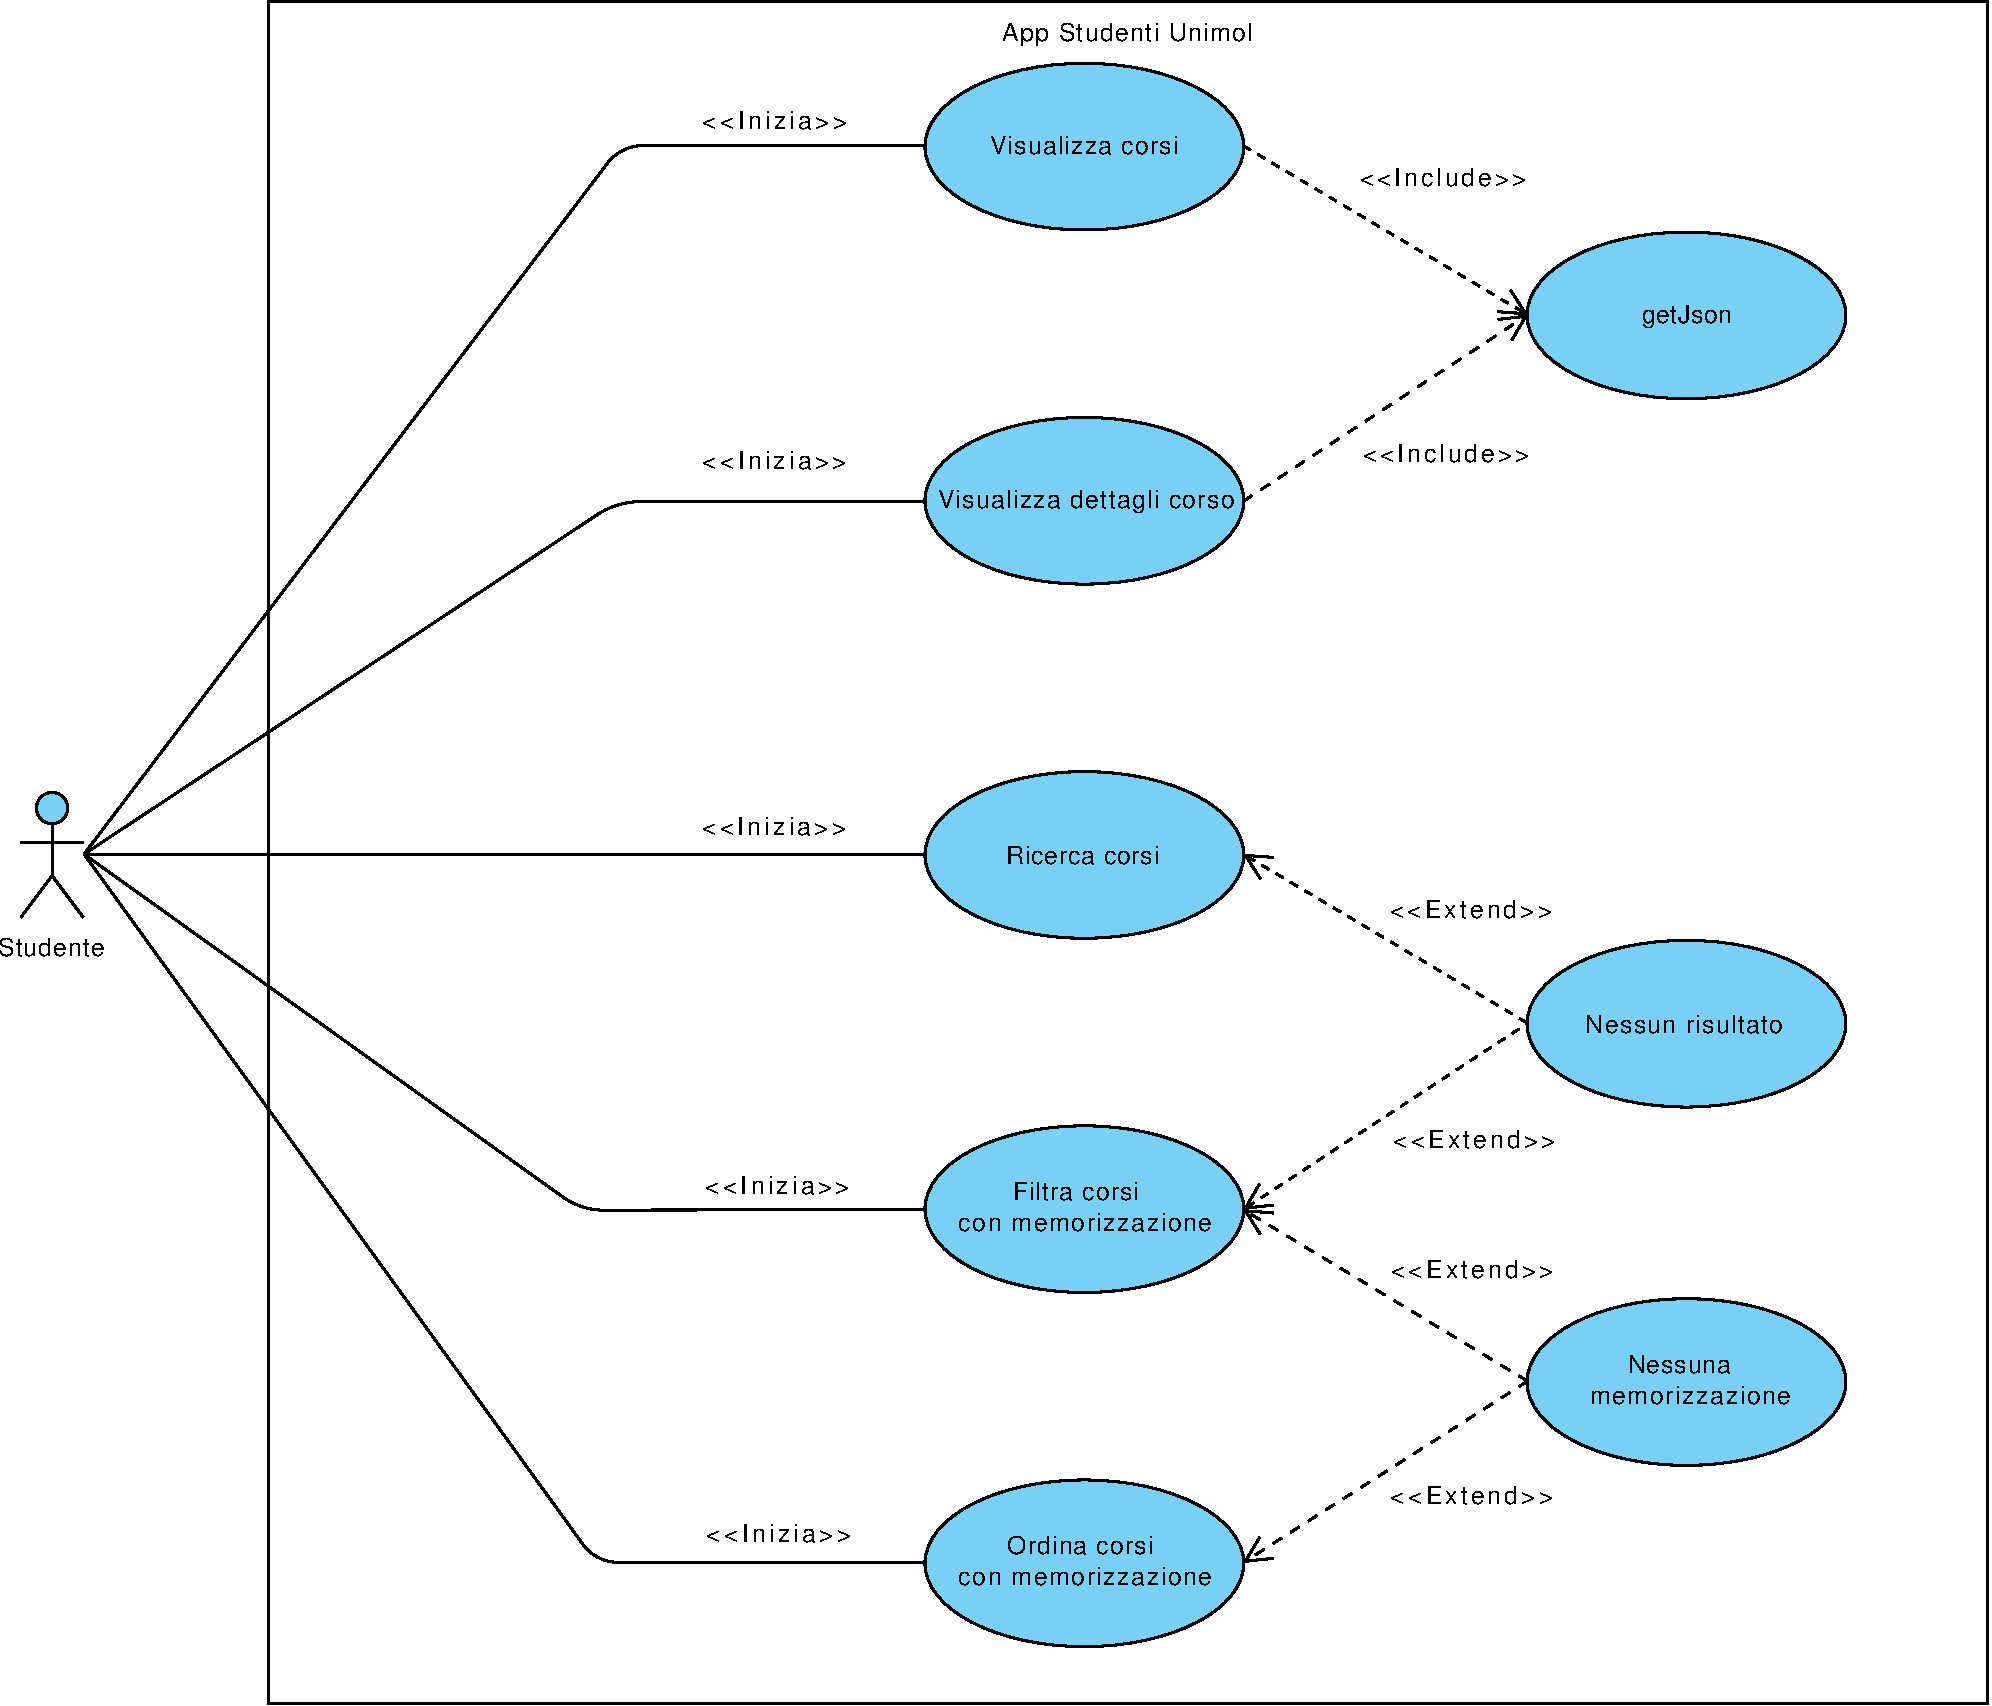
\includegraphics[width=6.5in]{imgs/gruppo1/use_case_diagrams/UCD1-gestione_piano_di_studio.pdf}
	\caption{Diagramma caso d'uso- Gestione piano di studio}
	\label{diag:gestionePianoStudio}
\end{figure}
\clearpage
\subsection{Funzionalità Visualizza dettagli corso}
\label{req:visualizzaDettagliCorso}
\paragraph{Visualizza dettagli corso \\}
Questo caso d’uso consentirà allo studente di visualizzare i dettagli di un corso e includerà il caso d’uso \textit{getJson} passandogli l’ID del servizio per ottenere i dettagli del corso selezionato. Quest’ultimo elaborerà la richiesta e restituirà i dati relativi al corso selezionato. Il sistema mostrerà allo studente i dettagli del corso selezionato. Segue il diagramma dei casi d'uso corrispondente a questo caso d'uso: \ref{diag:gestionePianoStudio}. È possibile prendere visione anche del diagramma di sequenza (\ref{diag:visualizzaDettagliCorsoSD}) e del diagramma delle attività (\ref{diag:visualizzaDettagliCorsoAD}). \\ \\
\begin{tabular}{| p{\useCaseLeft} | p{\useCaseNum} | p{\useCaseTwoCol} | p{\useCaseTwoCol} |}
	\hline
	\textbf{Nome caso d'uso} & \multicolumn{3}{p{\useCaseMulticol} |}{\textbf{Visualizza dettagli corso}} \\
	\hline
	\textbf{Attori partecipanti} & \multicolumn{3}{p{\useCaseMulticol} |}{Iniziato da \textit{Studente}.} \\
	\hline
	\textbf{Condizioni d'ingresso} & \multicolumn{3}{p{\useCaseMulticol} |}{Lo studente visualizza i corsi del piano di studio.} \\
	\hline
	\textbf{Flusso degli eventi} & \textbf{\#} & \textbf{Studente} & \textbf{Sistema} \\
	\hline
	\textbf{} & \textbf{1} & Seleziona un corso di cui visualizzare i dettagli. & \textbf{} \\
	\hline
	\textbf{} & \textbf{2} & \textbf{} & Include il caso d’uso \textit{getJson} passandogli l’ID del servizio. \\
	\hline
	\textbf{} & \textbf{3} & \textbf{} & Mostra i dettagli relativi al corso selezionato. \\
	\hline
	\textbf{Eccezioni} & \multicolumn{3}{p{\useCaseMulticol} |}{} \\
	\hline
	\textbf{Condizioni d'uscita} & \multicolumn{3}{p{\useCaseMulticol} |}{Lo studente visualizza i dettagli relativi al corso selezionato.} \\
	\hline
\end{tabular}

\clearpage

\subsection{Funzionalità Gestione appelli}
\clearpage
%\paragraph{Visualizza appelli disponibil}
\begin{figure}
	\centering
	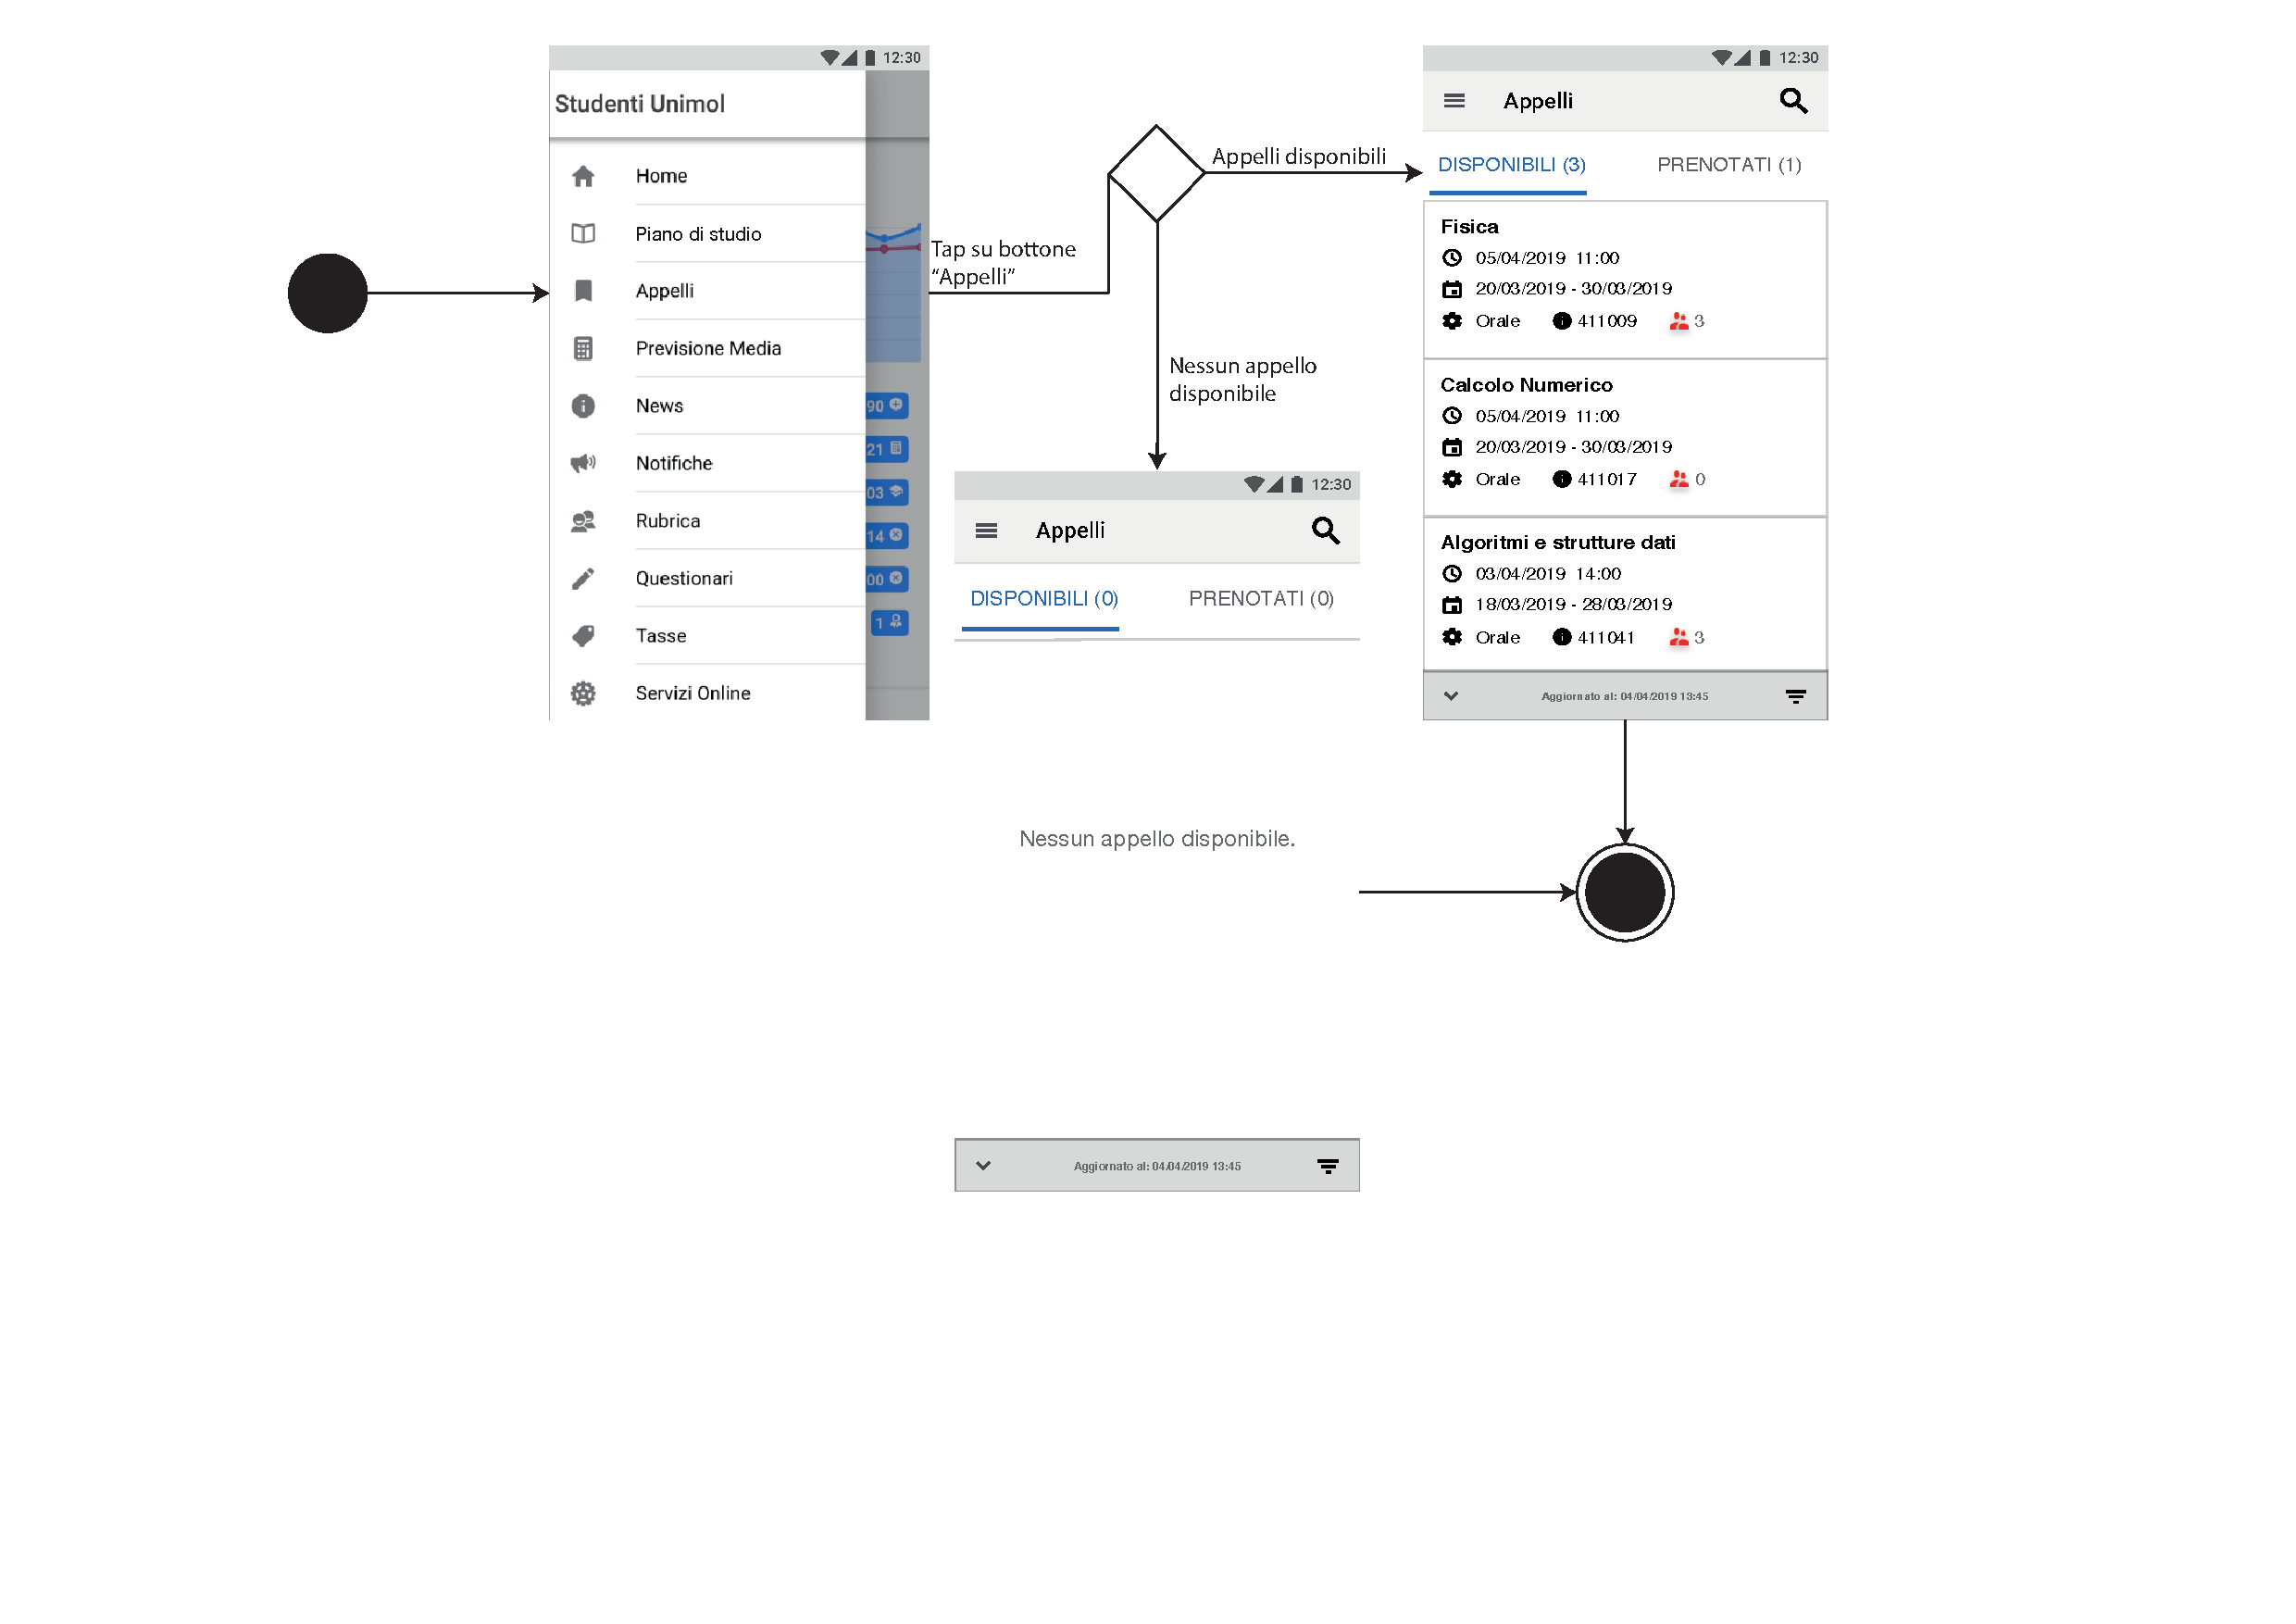
\includegraphics[width=6in]{imgs/gruppo1/activity_diagrams/AD6_visualizza_appelli_disponibili.pdf}
	\caption{Activity Diagram - Visualizza appelli disponibili}
	\label{diag:visualizzaAppelliDisponibiliAD}
\end{figure}
\newpage

%\paragraph{Visualizza appelli prenotati}
\begin{figure}
	\centering
	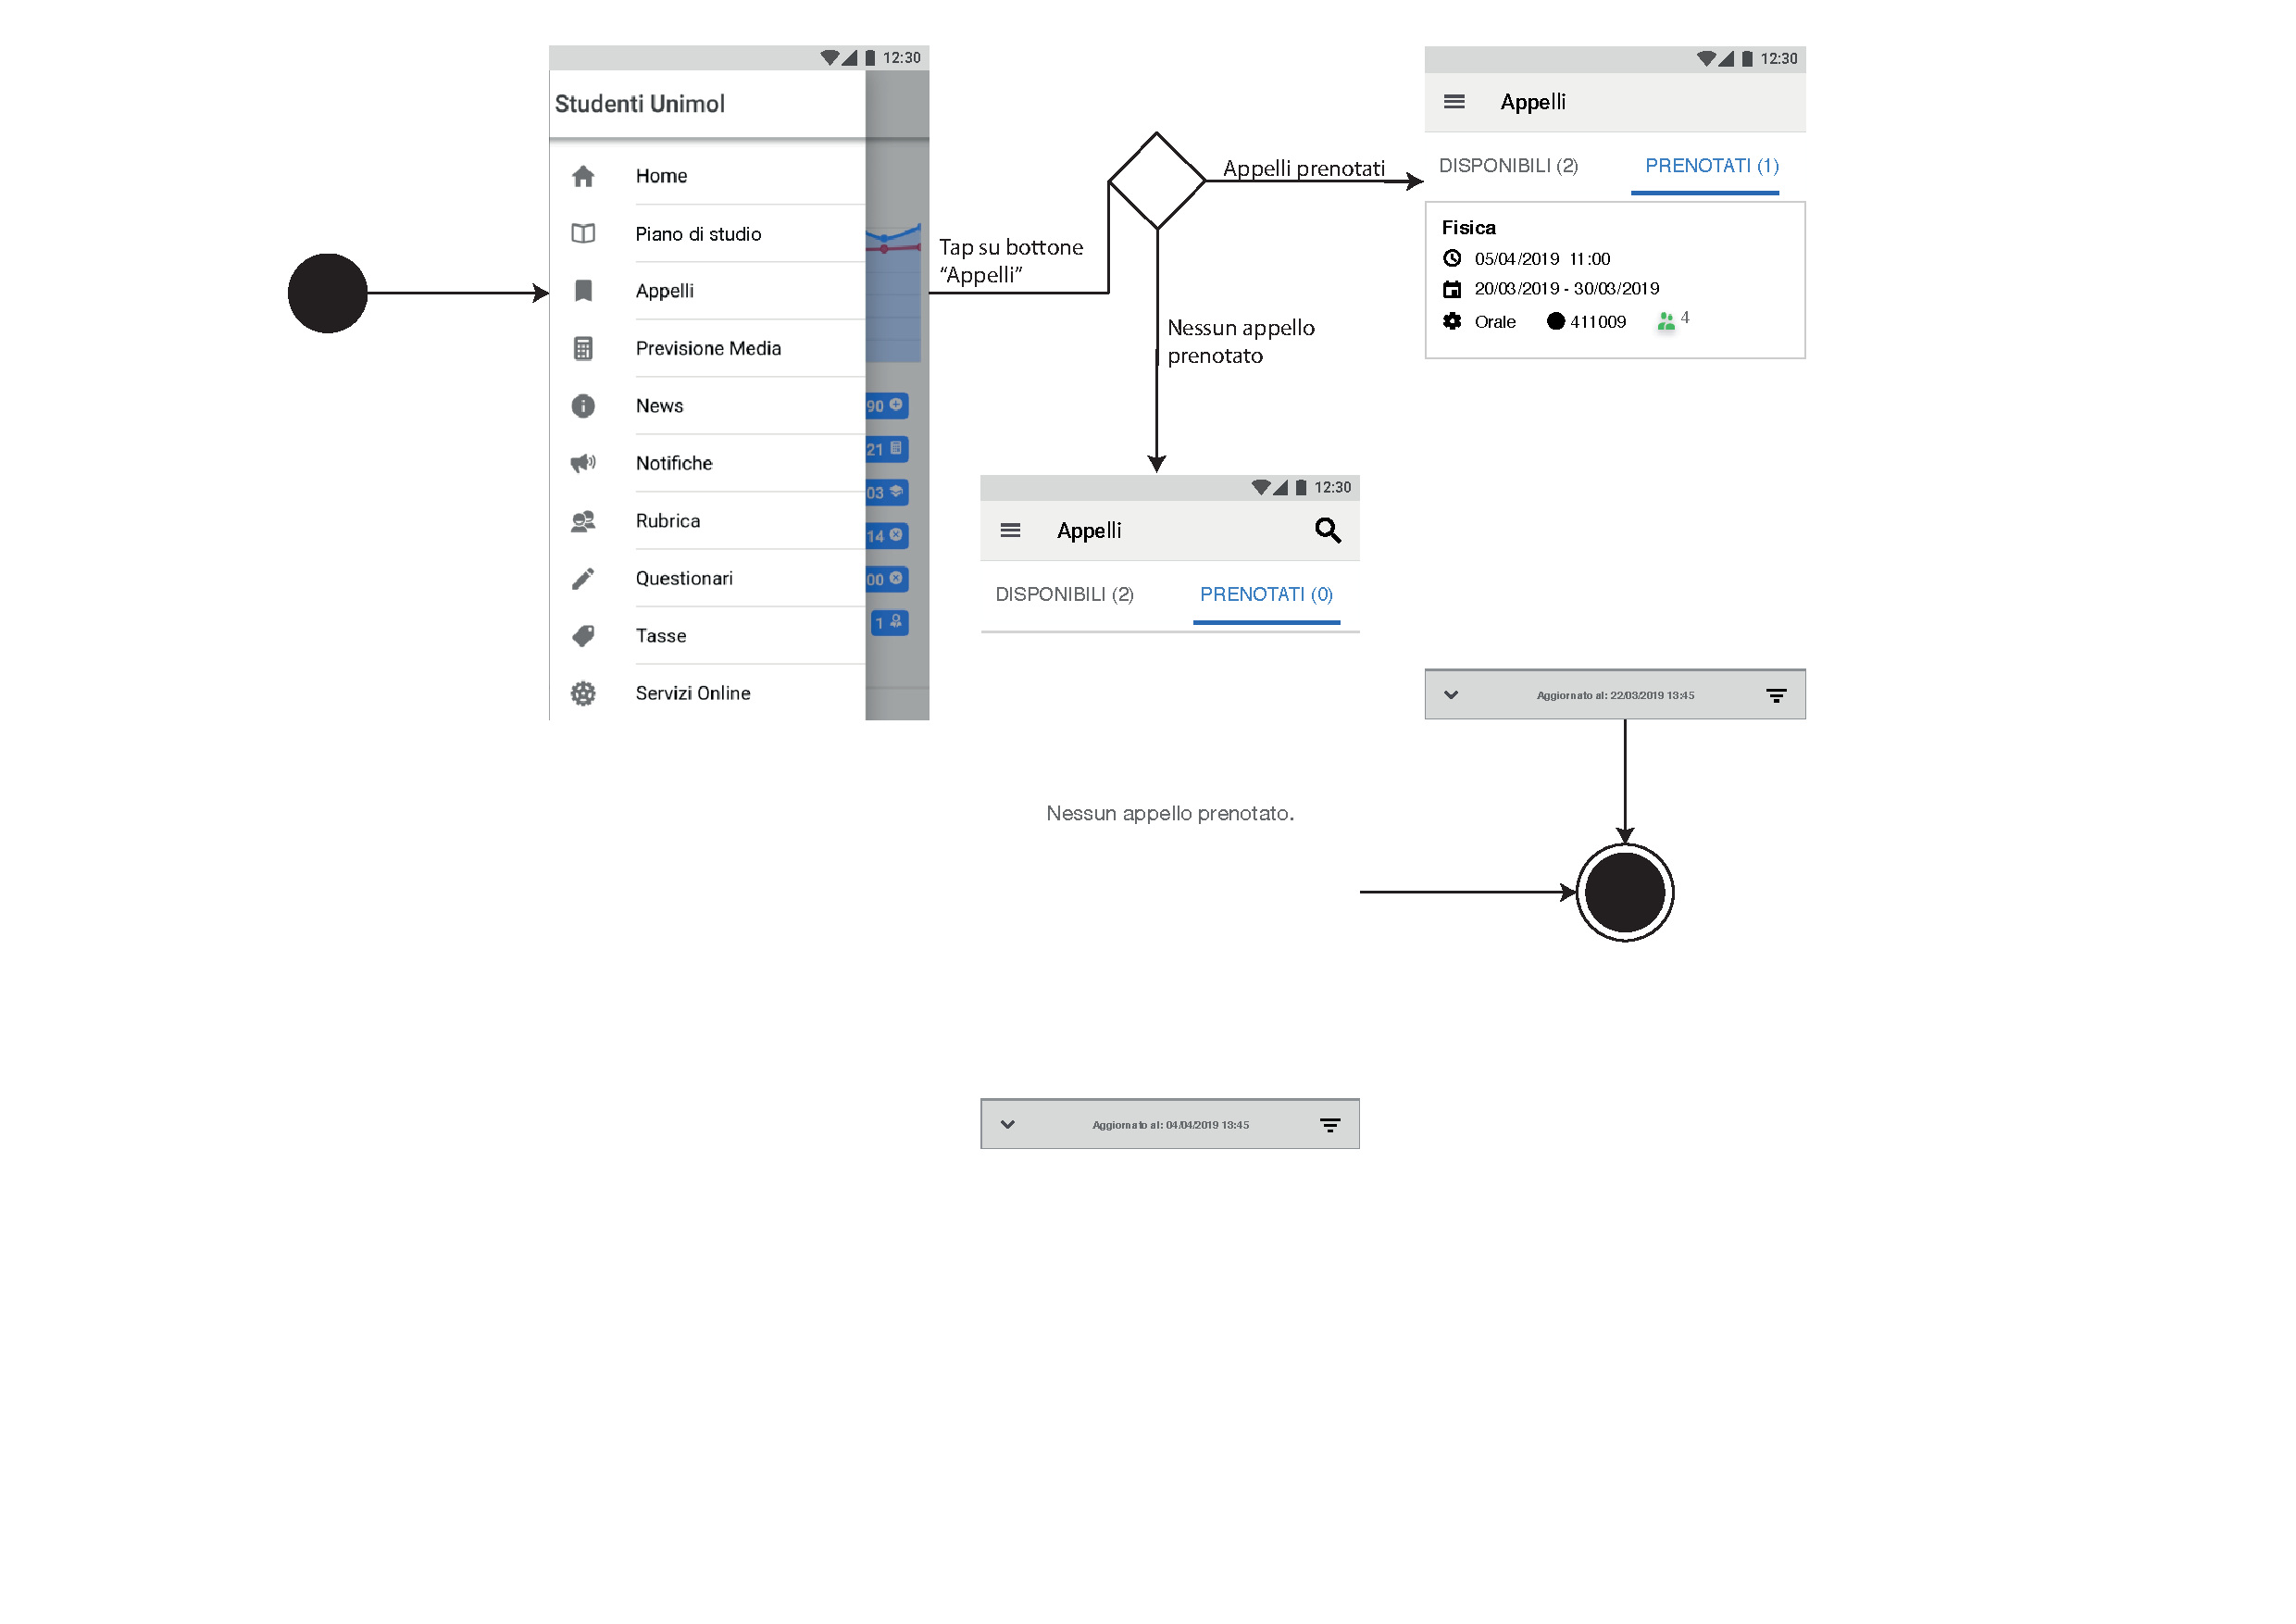
\includegraphics[width=6in]{imgs/gruppo1/activity_diagrams/AD7_visualizza_appelli_prenotati.pdf}
	\caption{Activity Diagram - Visualizza appelli prenotati}
	\label{diag:visualizzaAppelliPrenotatiAD}
\end{figure}
\newpage

%\paragraph{Ricerca appelli disponibili}
\begin{figure}
	\centering
	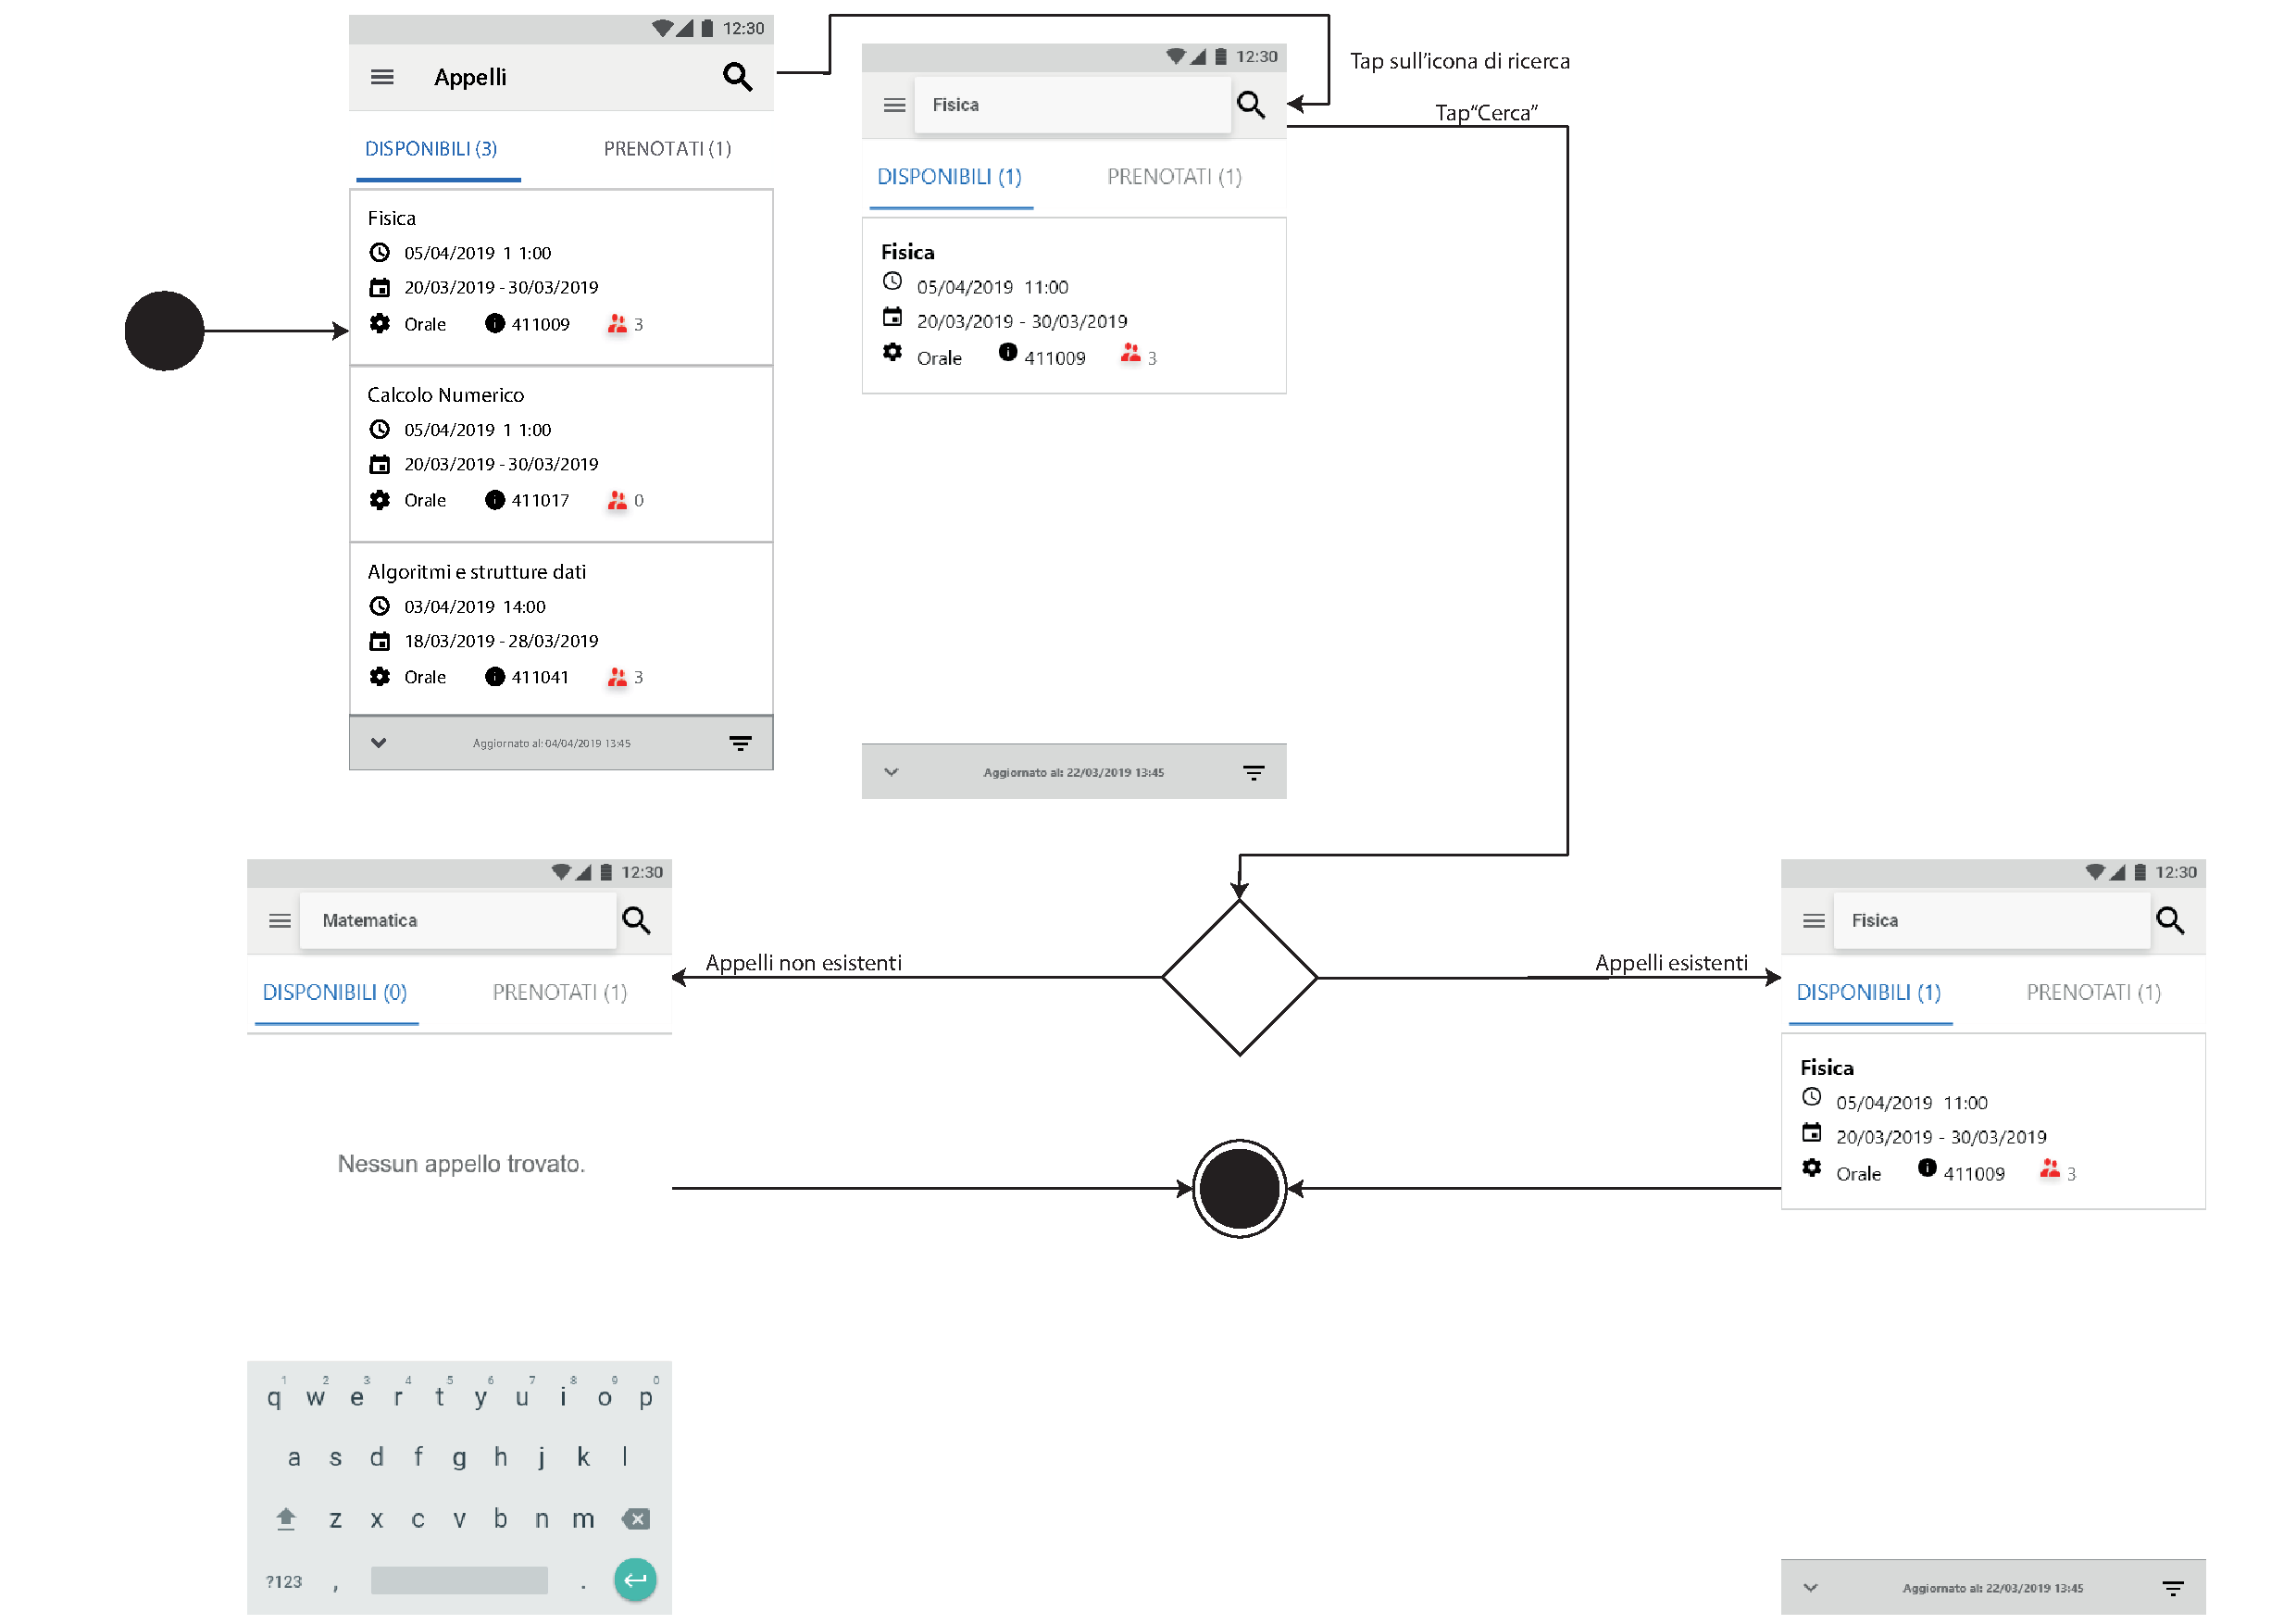
\includegraphics[width=6in]{imgs/gruppo1/activity_diagrams/AD8_Ricerca_appelli.pdf}
	\caption{Activity Diagram - Ricerca appelli disponibili}
	\label{diag:ricercaAppelliDisponibiliAD}
\end{figure}
\newpage

%\paragraph{Filtra appelli disponibili con memorizzazione }
\begin{figure}
	\centering
	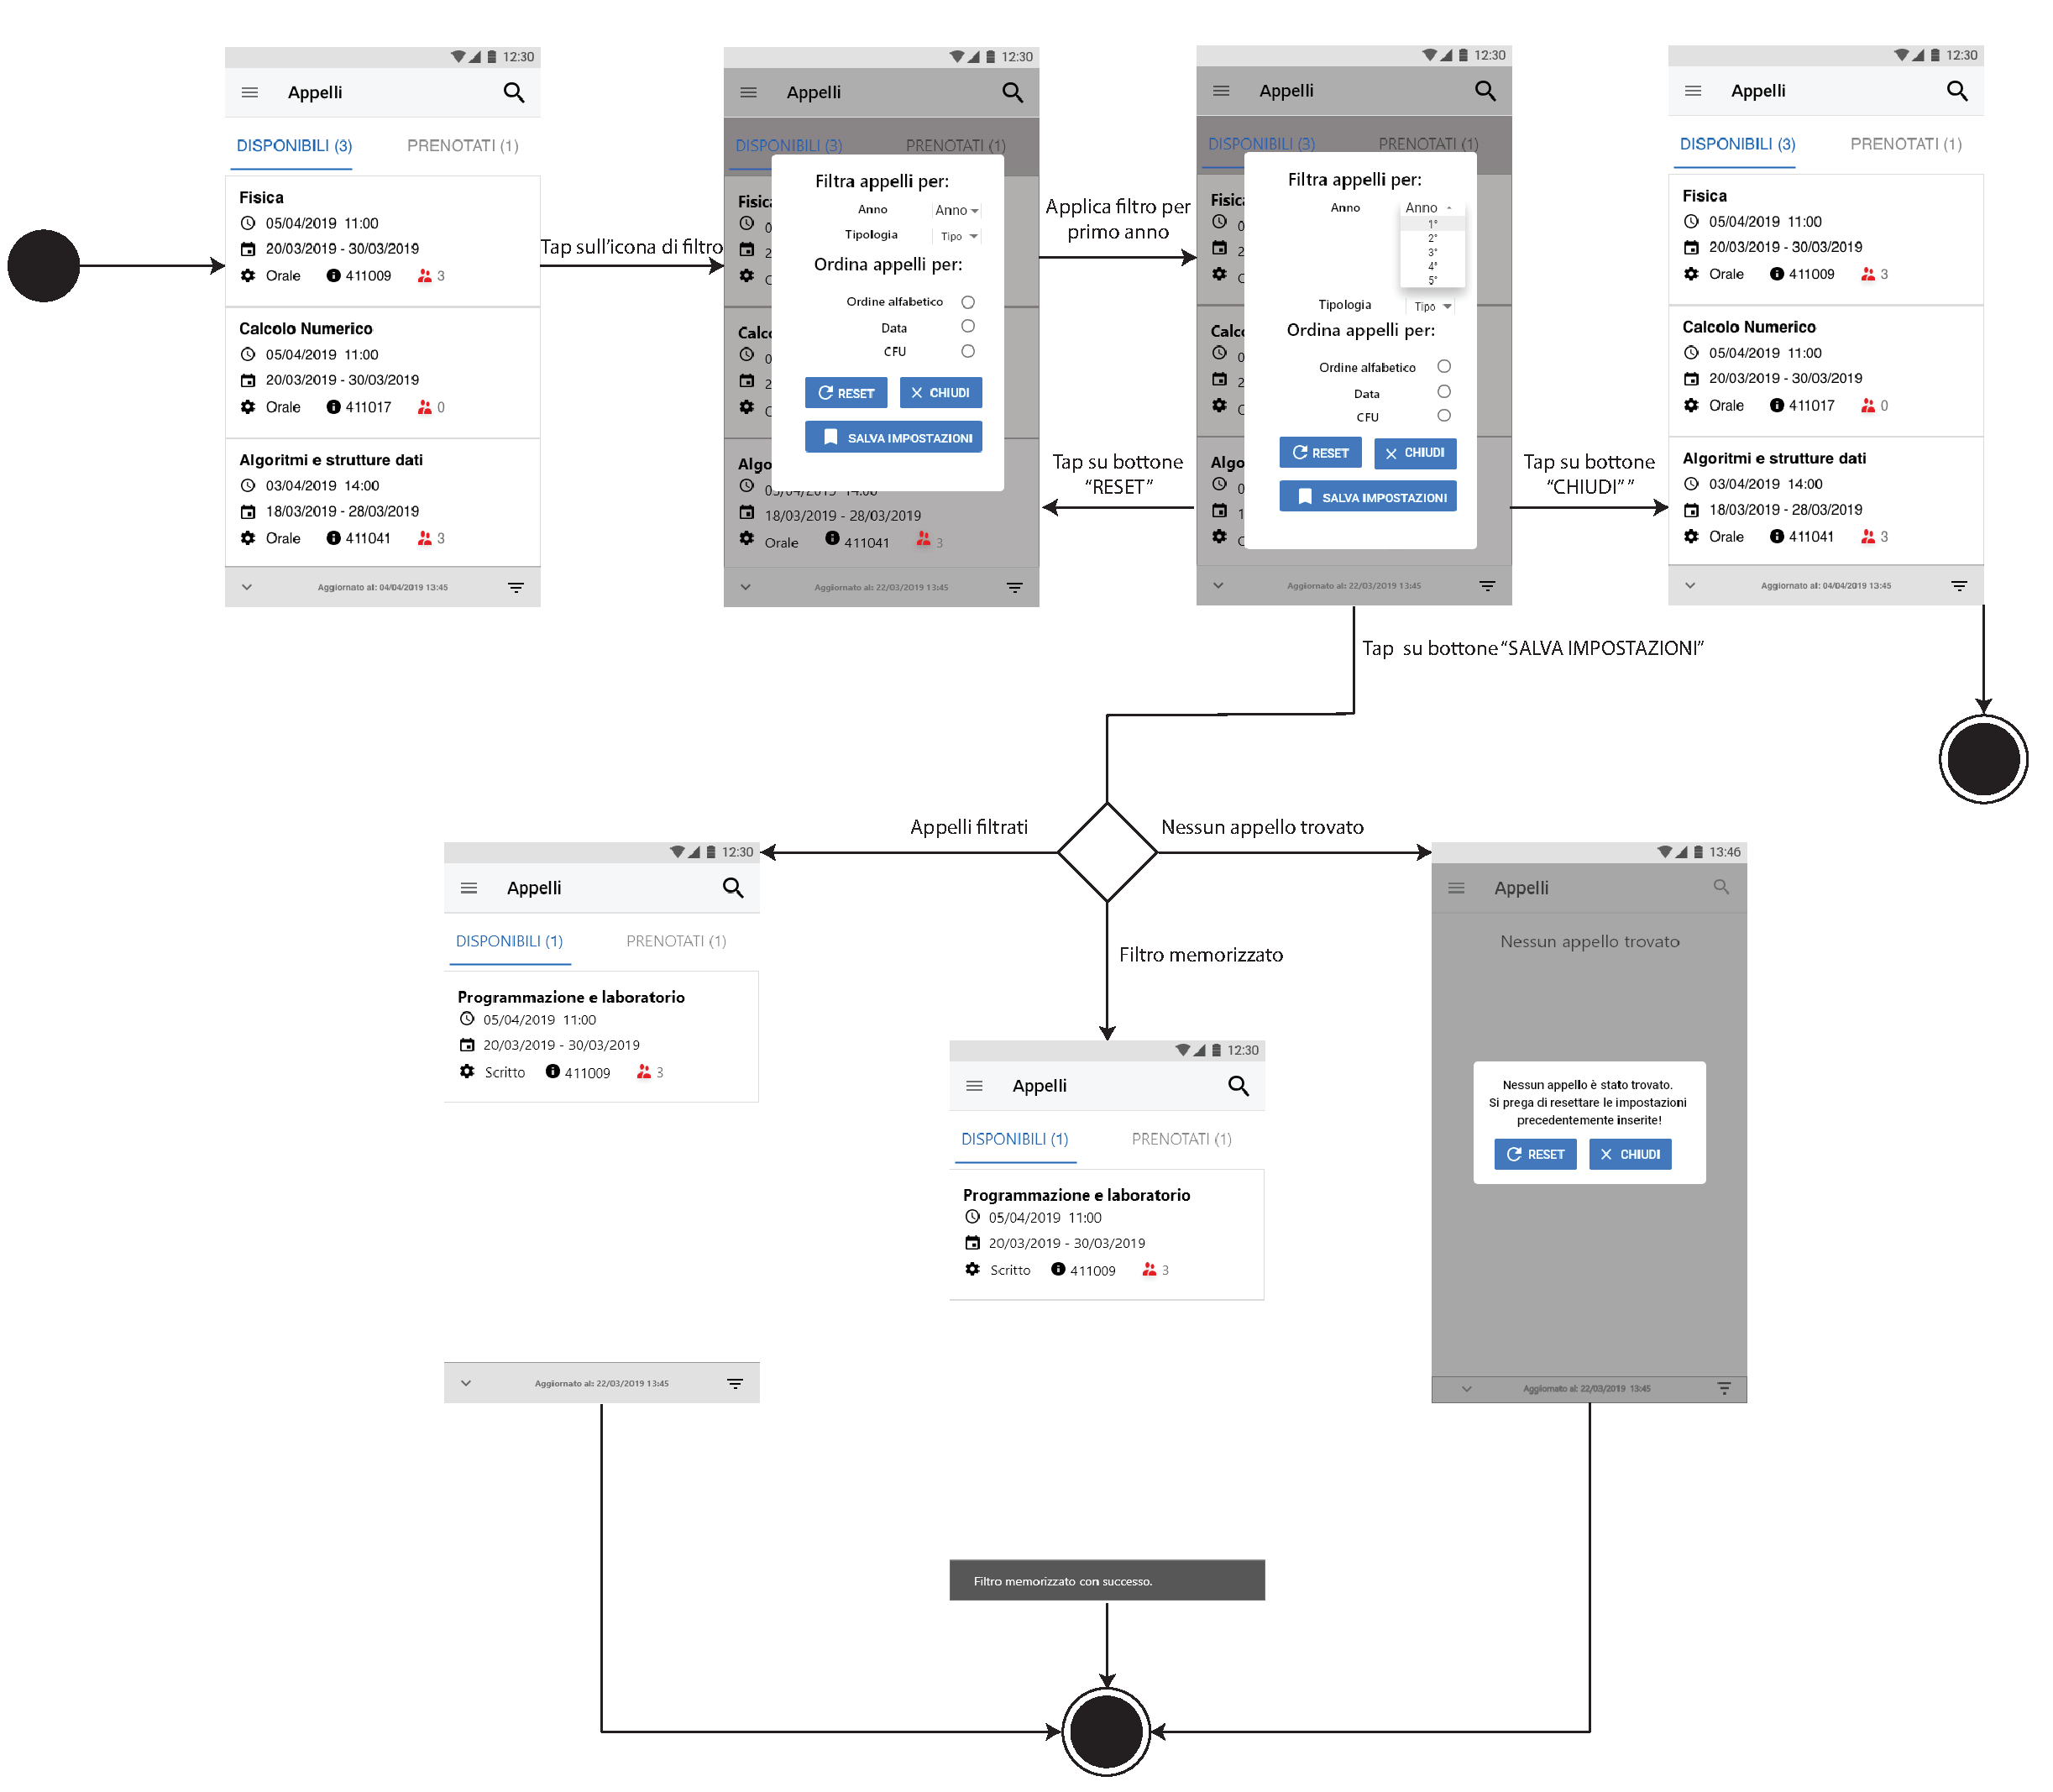
\includegraphics[width=6in]{imgs/gruppo1/activity_diagrams/AD9_filtrati_appelli.pdf}
	\caption{Activity Diagram - Filtra appelli disponibili con memorizzazione}
	\label{diag:filtraAppelliDisponibiliConMemAD}
\end{figure}
\newpage

%\paragraph{Ordina appelli disponibili con memorizzazione }
\begin{figure}
	\centering
	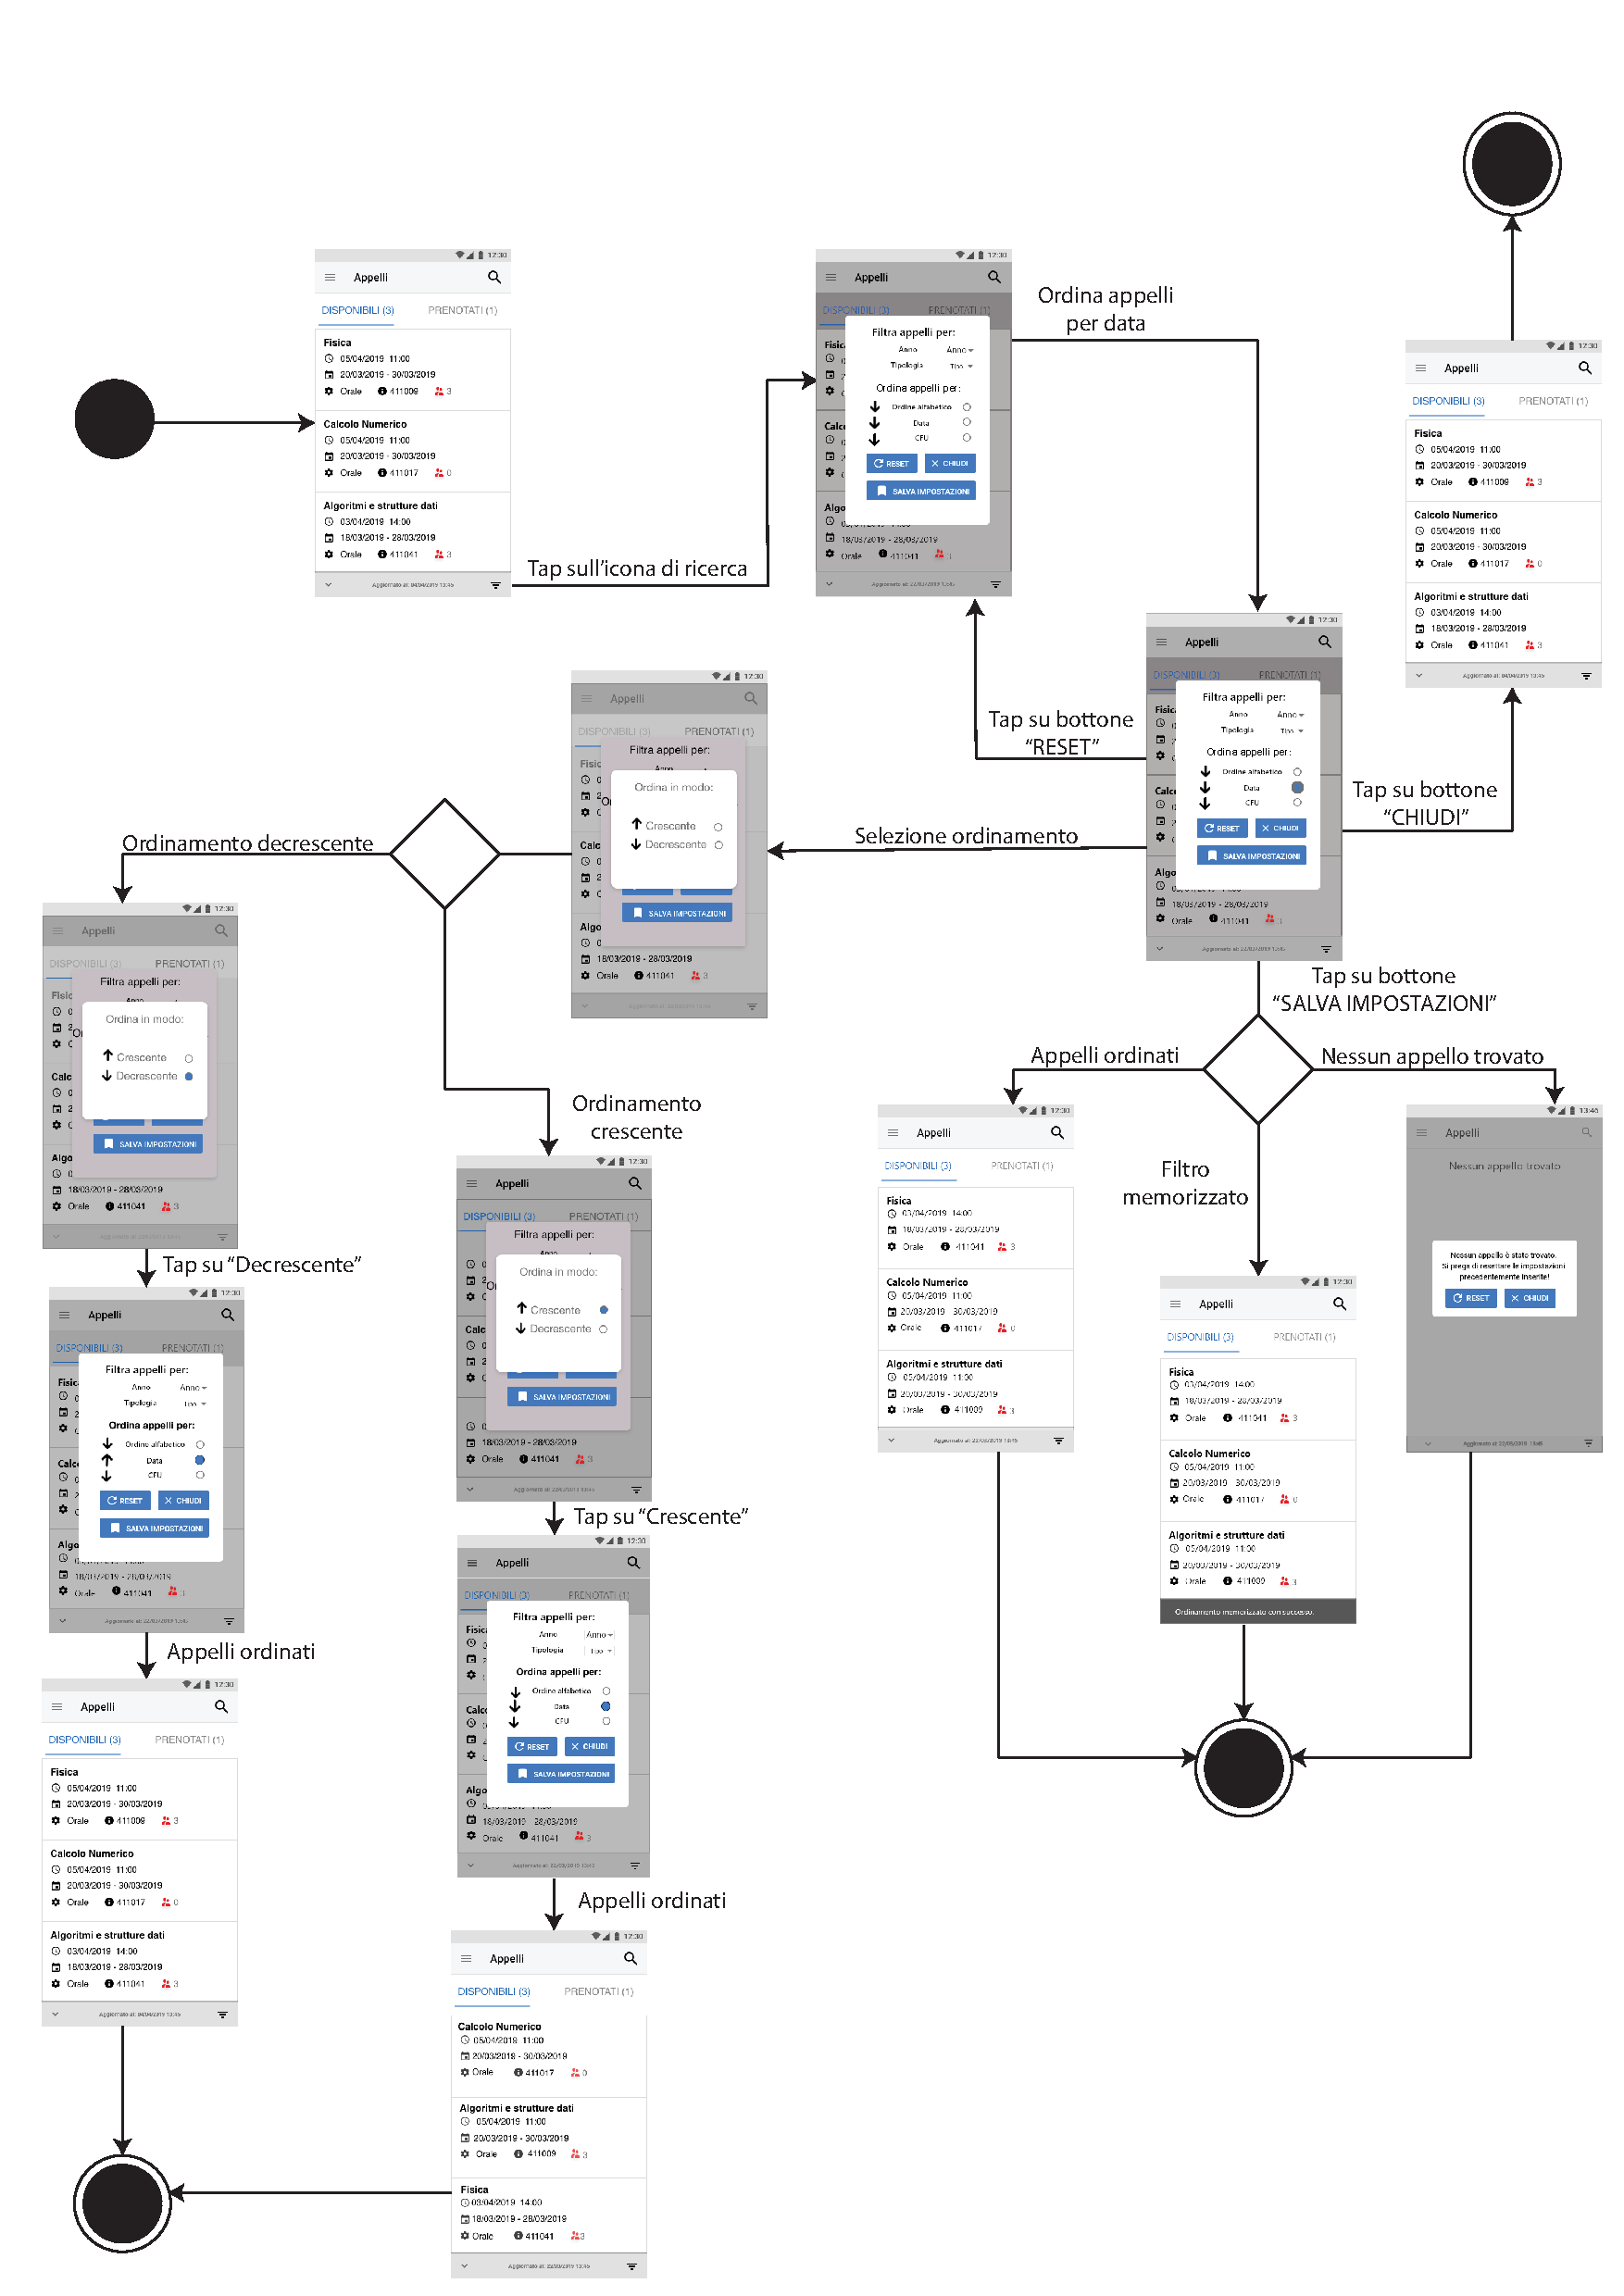
\includegraphics[width=6in]{imgs/gruppo1/activity_diagrams/AD10_ordina_appelli.pdf}
	\caption{Activity Diagram - Ordina appelli disponibili con memorizzazione}
	\label{diag:ordinaAppelliDisponibiliConMemAD}
\end{figure}
\newpage

%\paragraph{Prenota appello }
\begin{figure}
	\centering
	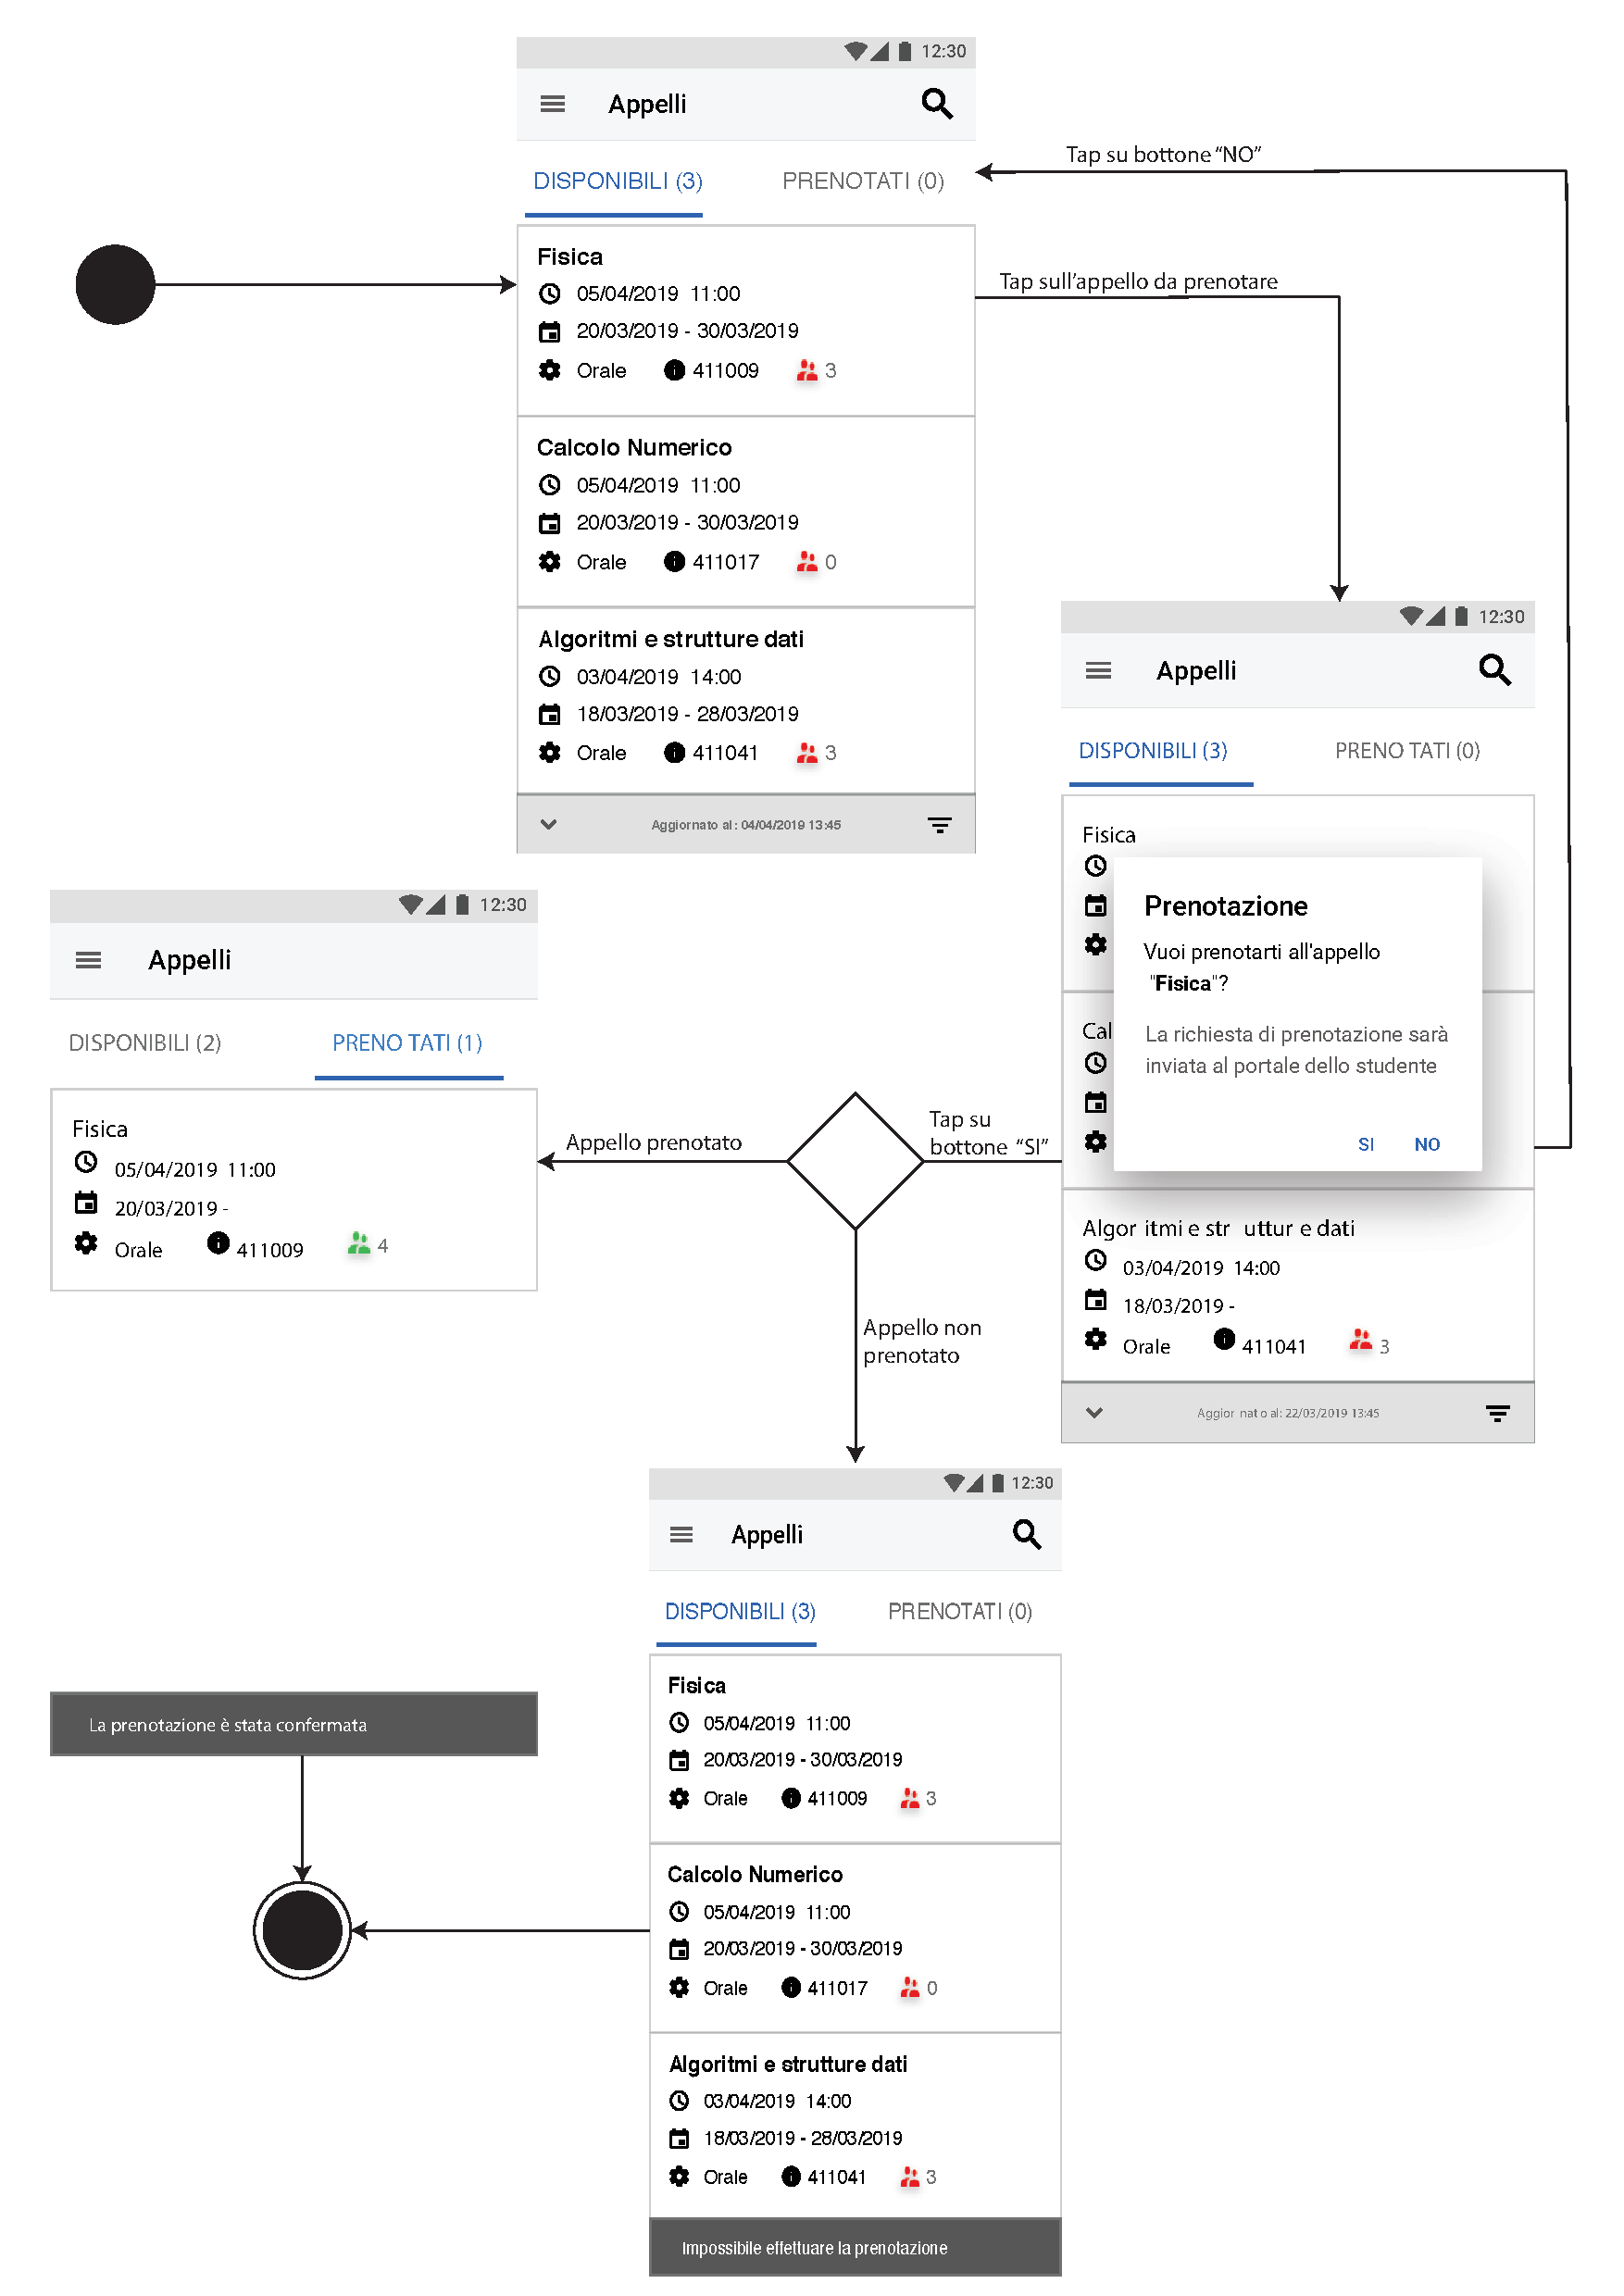
\includegraphics[width=6in]{imgs/gruppo1/activity_diagrams/AD11_prenota_apppello.pdf}
	\caption{Activity Diagram - Prenota appello}
	\label{diag:prenotaAppelloAD}
\end{figure}
\newpage

%\paragraph{Cancella prenotazione}
\begin{figure}
	\centering
	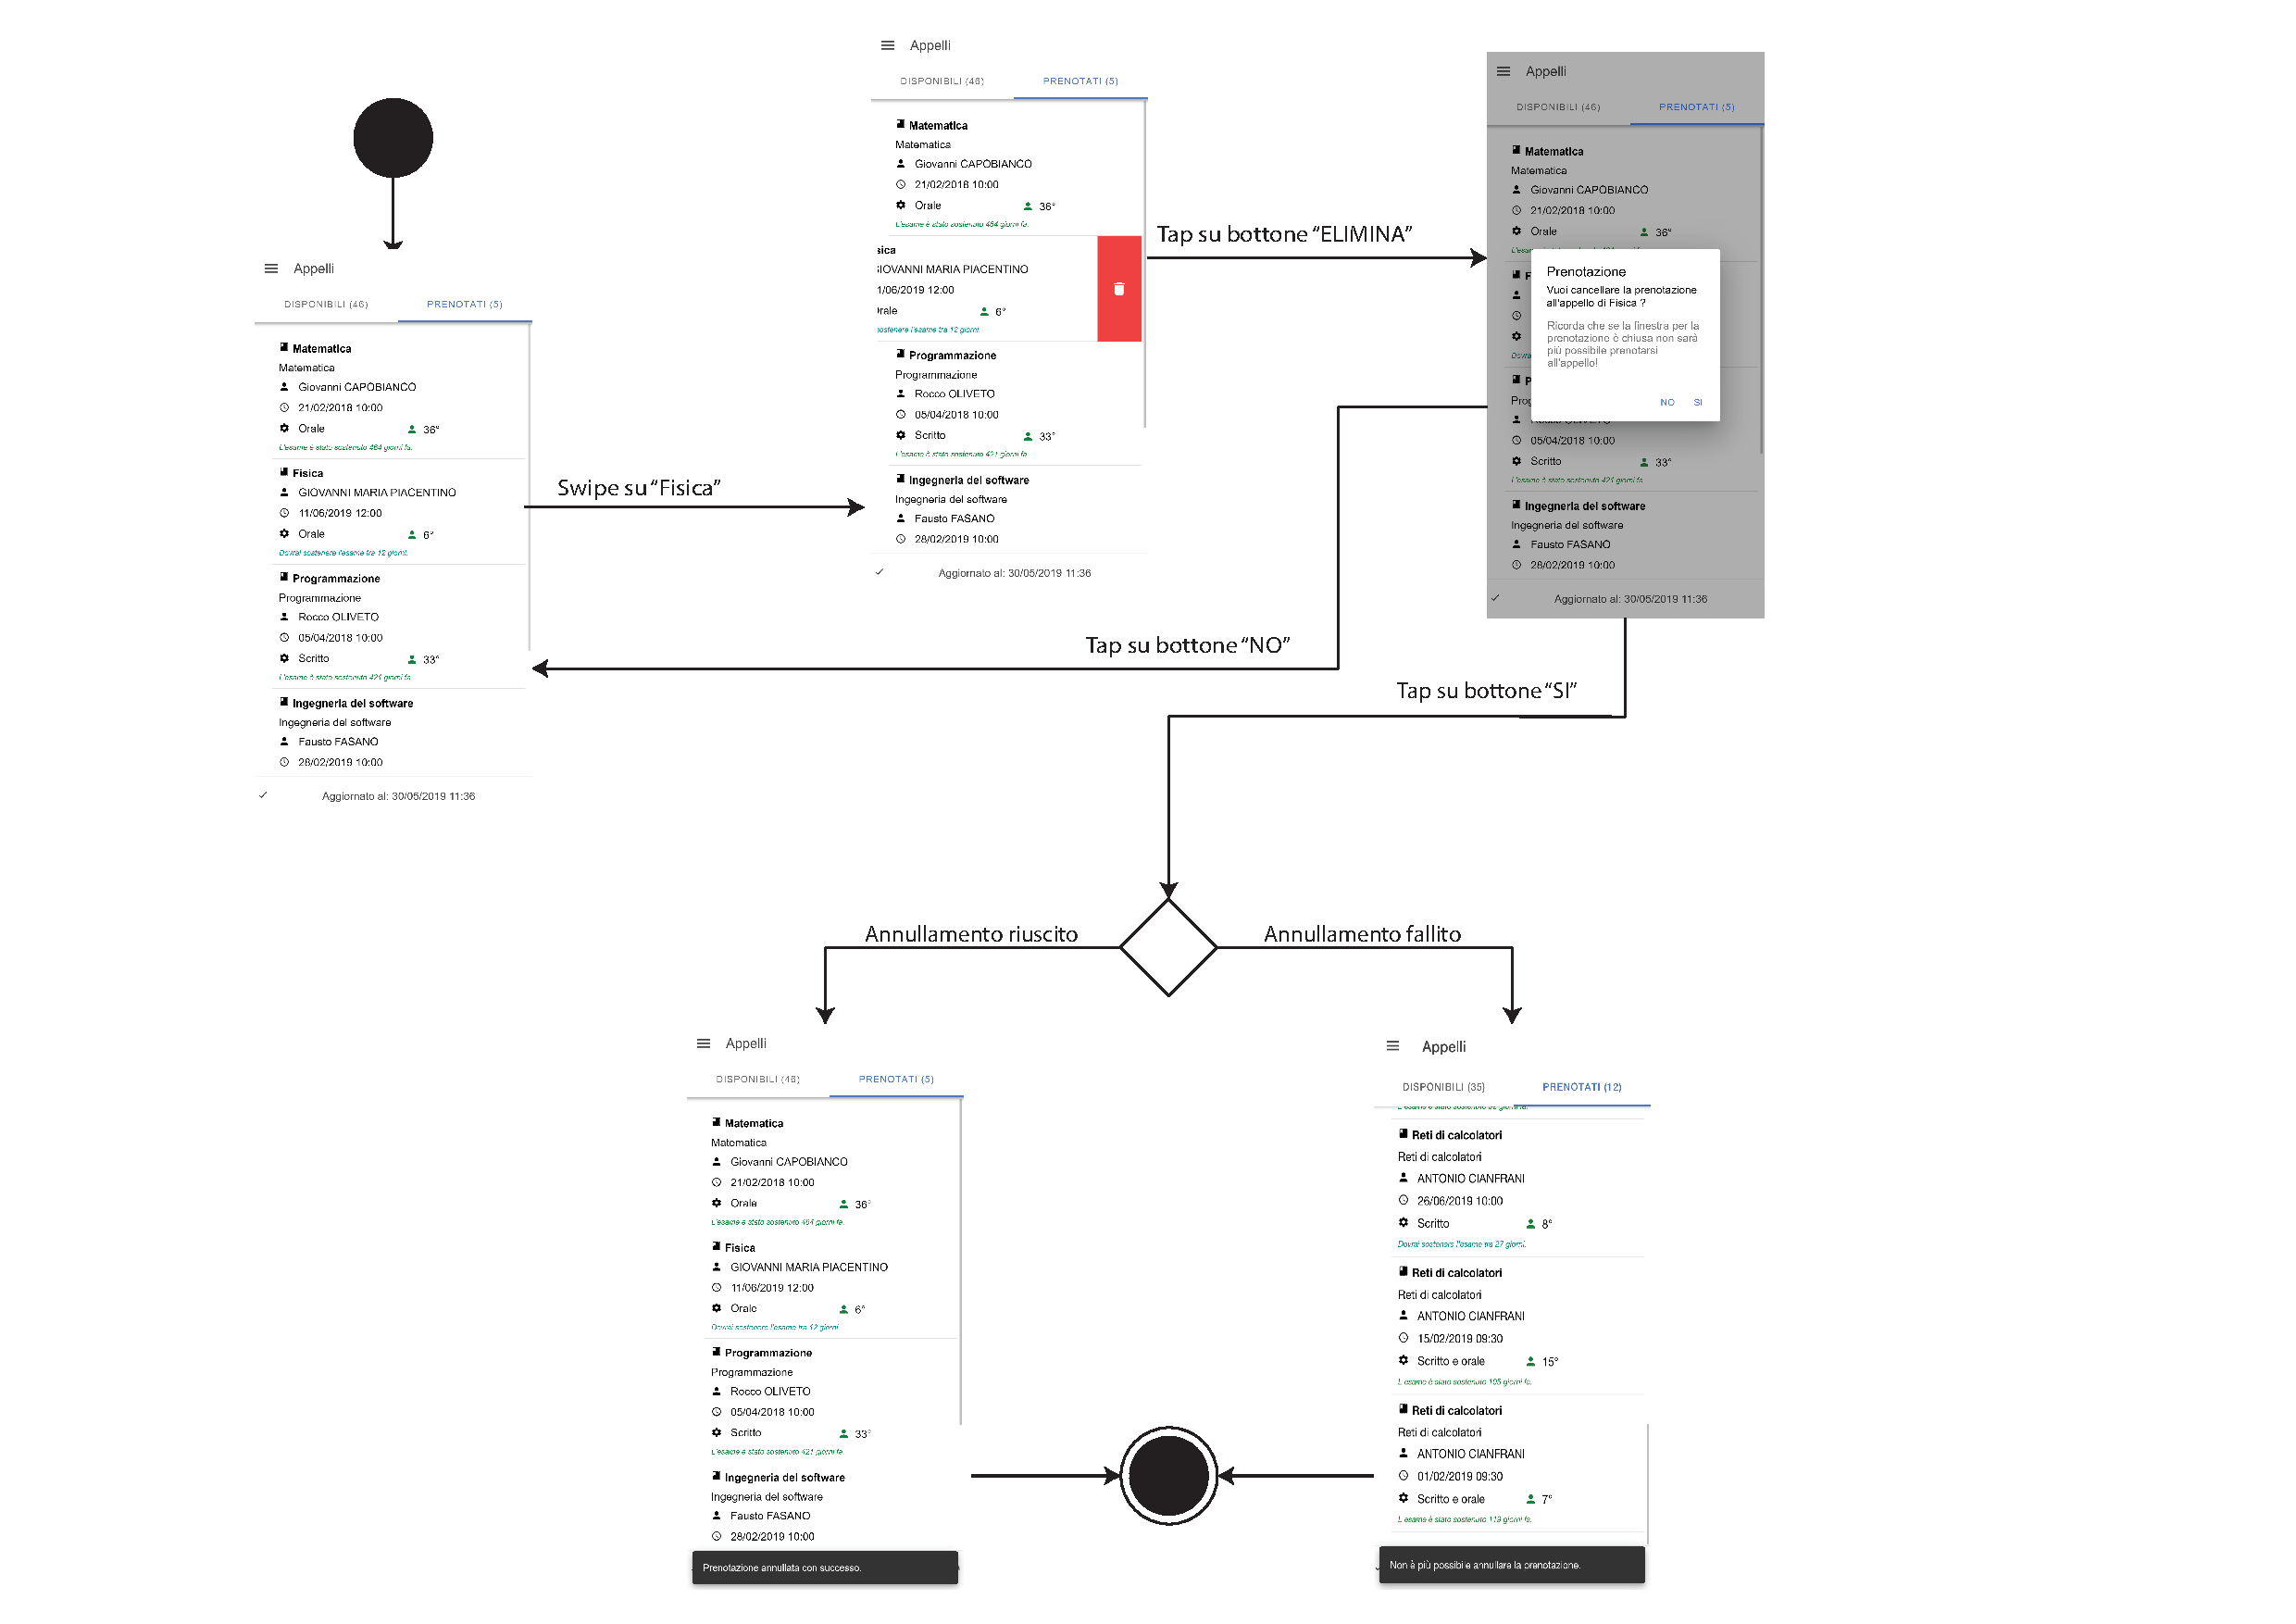
\includegraphics[width=6in]{imgs/gruppo1/activity_diagrams/AD12_cancella_prenotazione.pdf}
<<<<<<< HEAD
	\caption{Activity Diagram - Cancella Prenotazione}
	\label{diag:cancellaPrenotazioneAD}
\end{figure}

\clearpage
\subsection{Funzionalità Gestione materiale didattico}

%\paragraph{Visualizza elenco file}
\begin{figure}
	\centering
	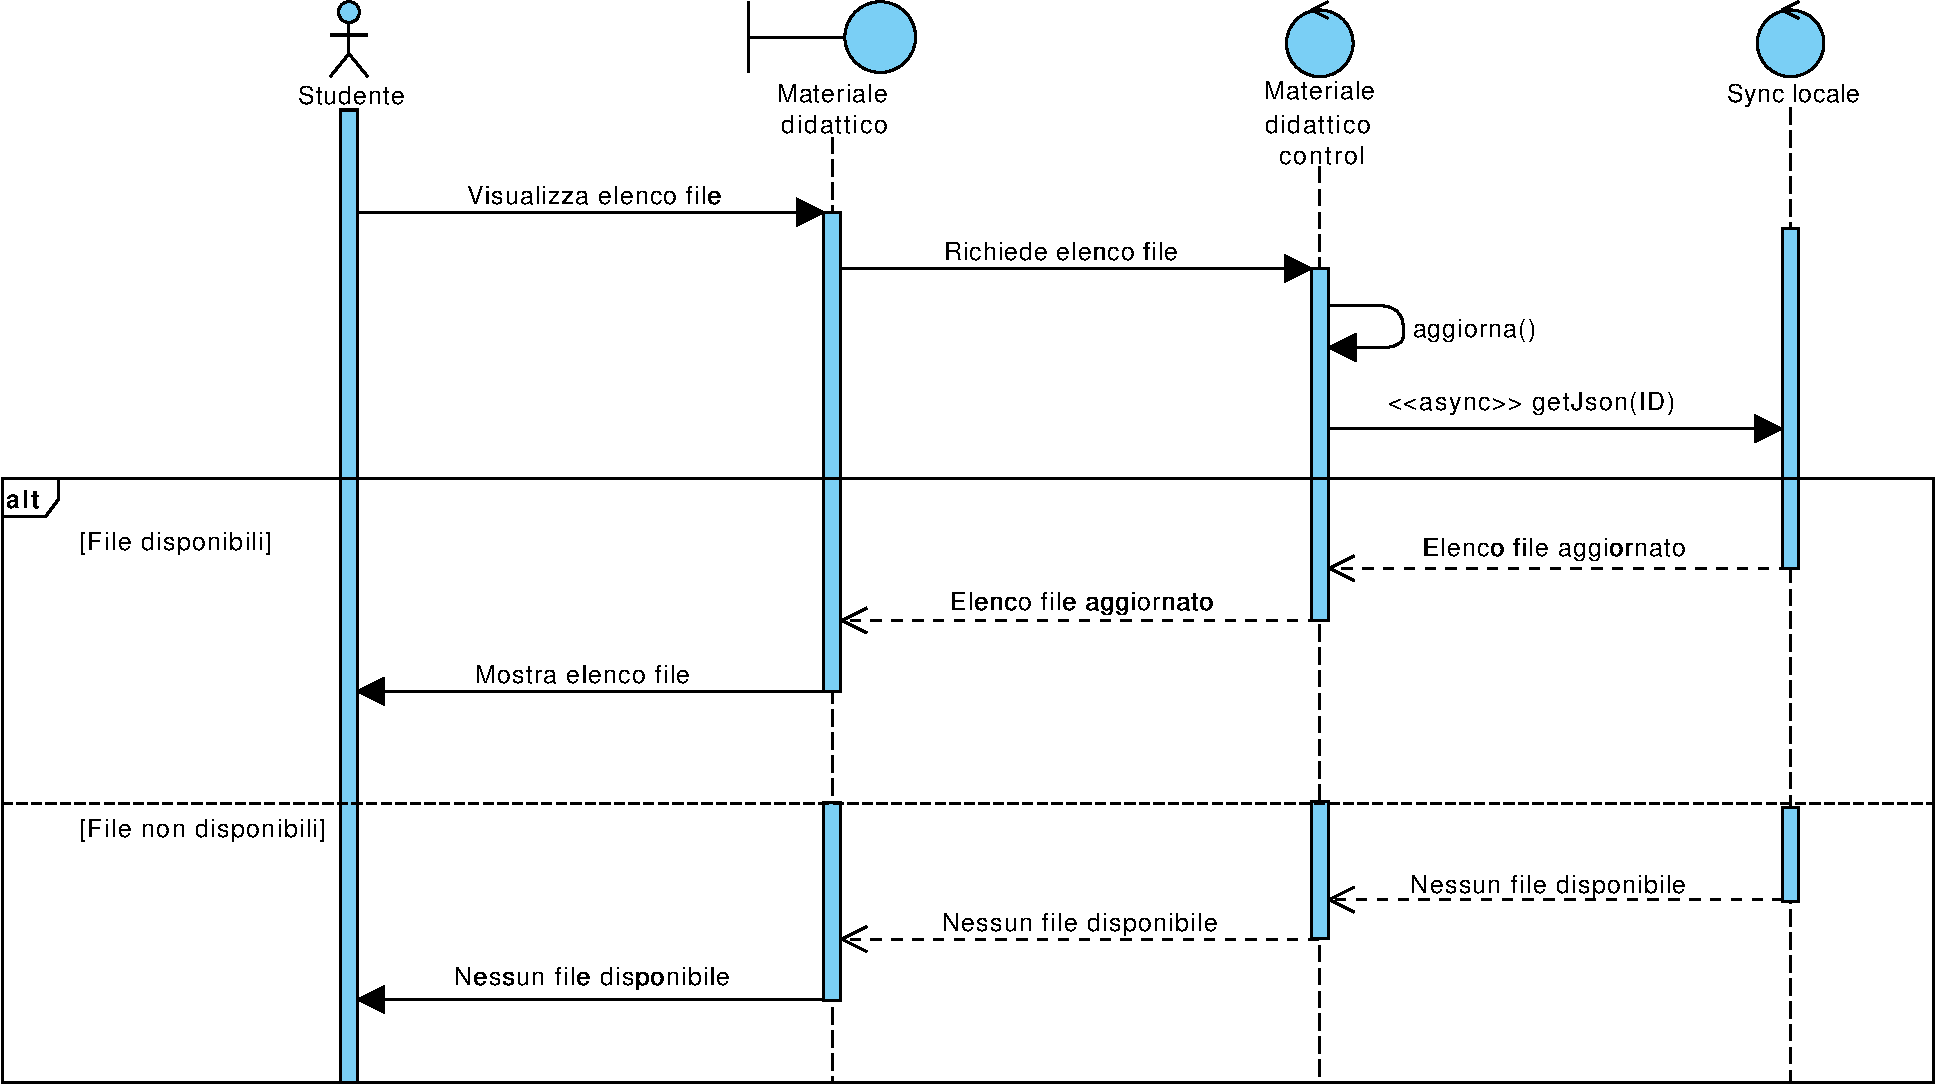
\includegraphics[width=6.5in]{imgs/gruppo1/sequence_diagrams/SD13_visualizza_elenco_file.pdf}
	\caption{Sequence Diagram - Visualizza elenco file}
	\label{diag:visualizzaElencoFileSD}
\end{figure}

%% 8.5.14 - Ricerca file %
\paragraph{Ricerca file}
\begin{figure}
	\centering
	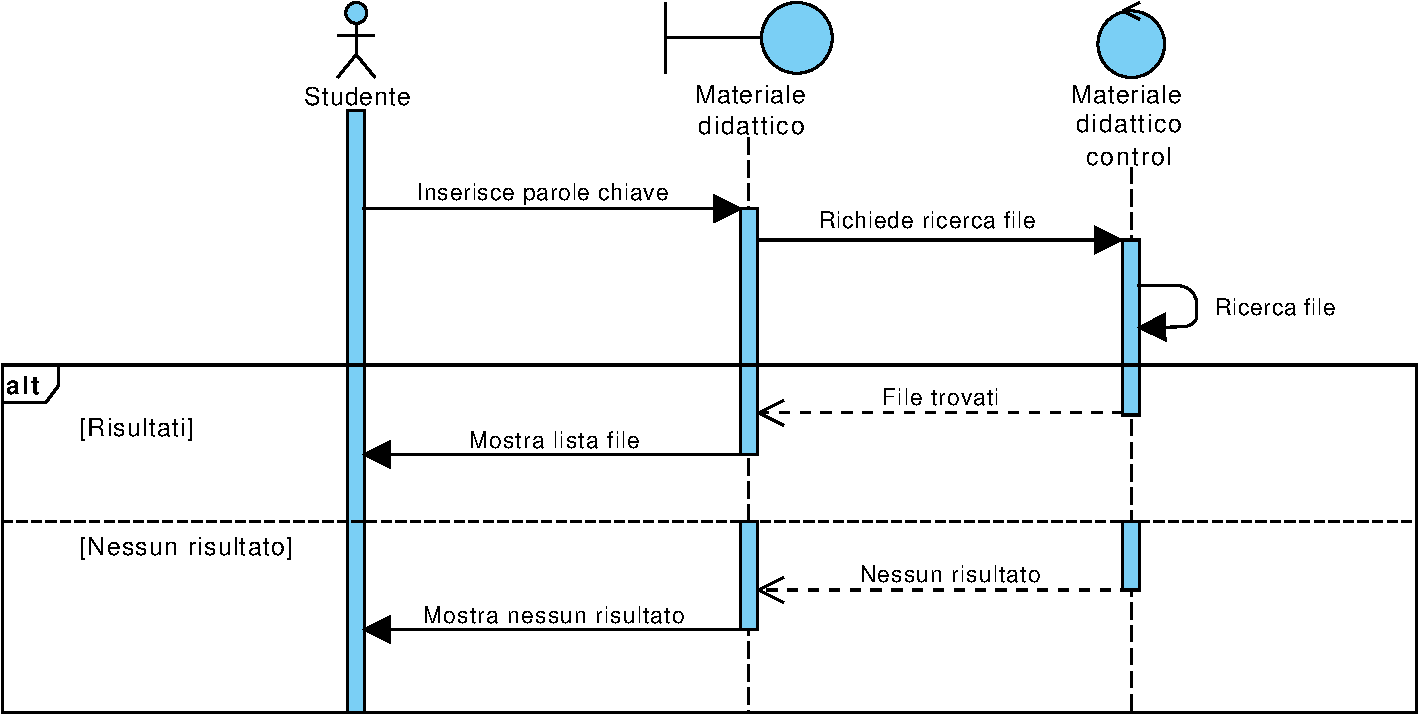
\includegraphics[width=6.5in]{imgs/gruppo1/sequence_diagrams/SD14_ricerca_file.pdf}
	\caption{Sequence Diagram - Ricerca file}
	\label{diag:ricercaFileSD}
\end{figure}
\newpage

%\paragraph{Visualizza dettagli file}
\begin{figure}
	\centering
	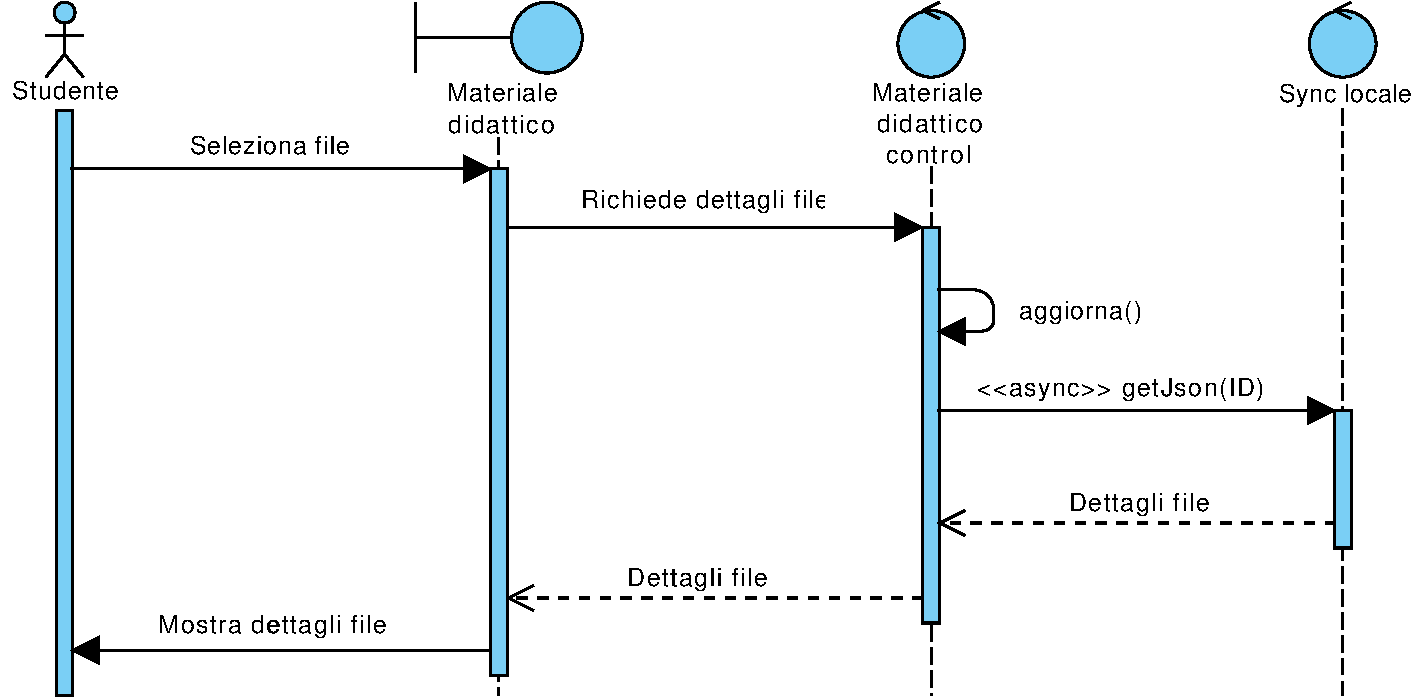
\includegraphics[width=6.5in]{imgs/gruppo1//sequence_diagrams/SD15_visualizza_dettagli_file.pdf}
	\caption{Sequence Diagram - Visualizza dettagli file}
	\label{diag:visualizzaDettagliFileSD}
\end{figure}

%\paragraph{Apri file}
\begin{figure}
	\centering
	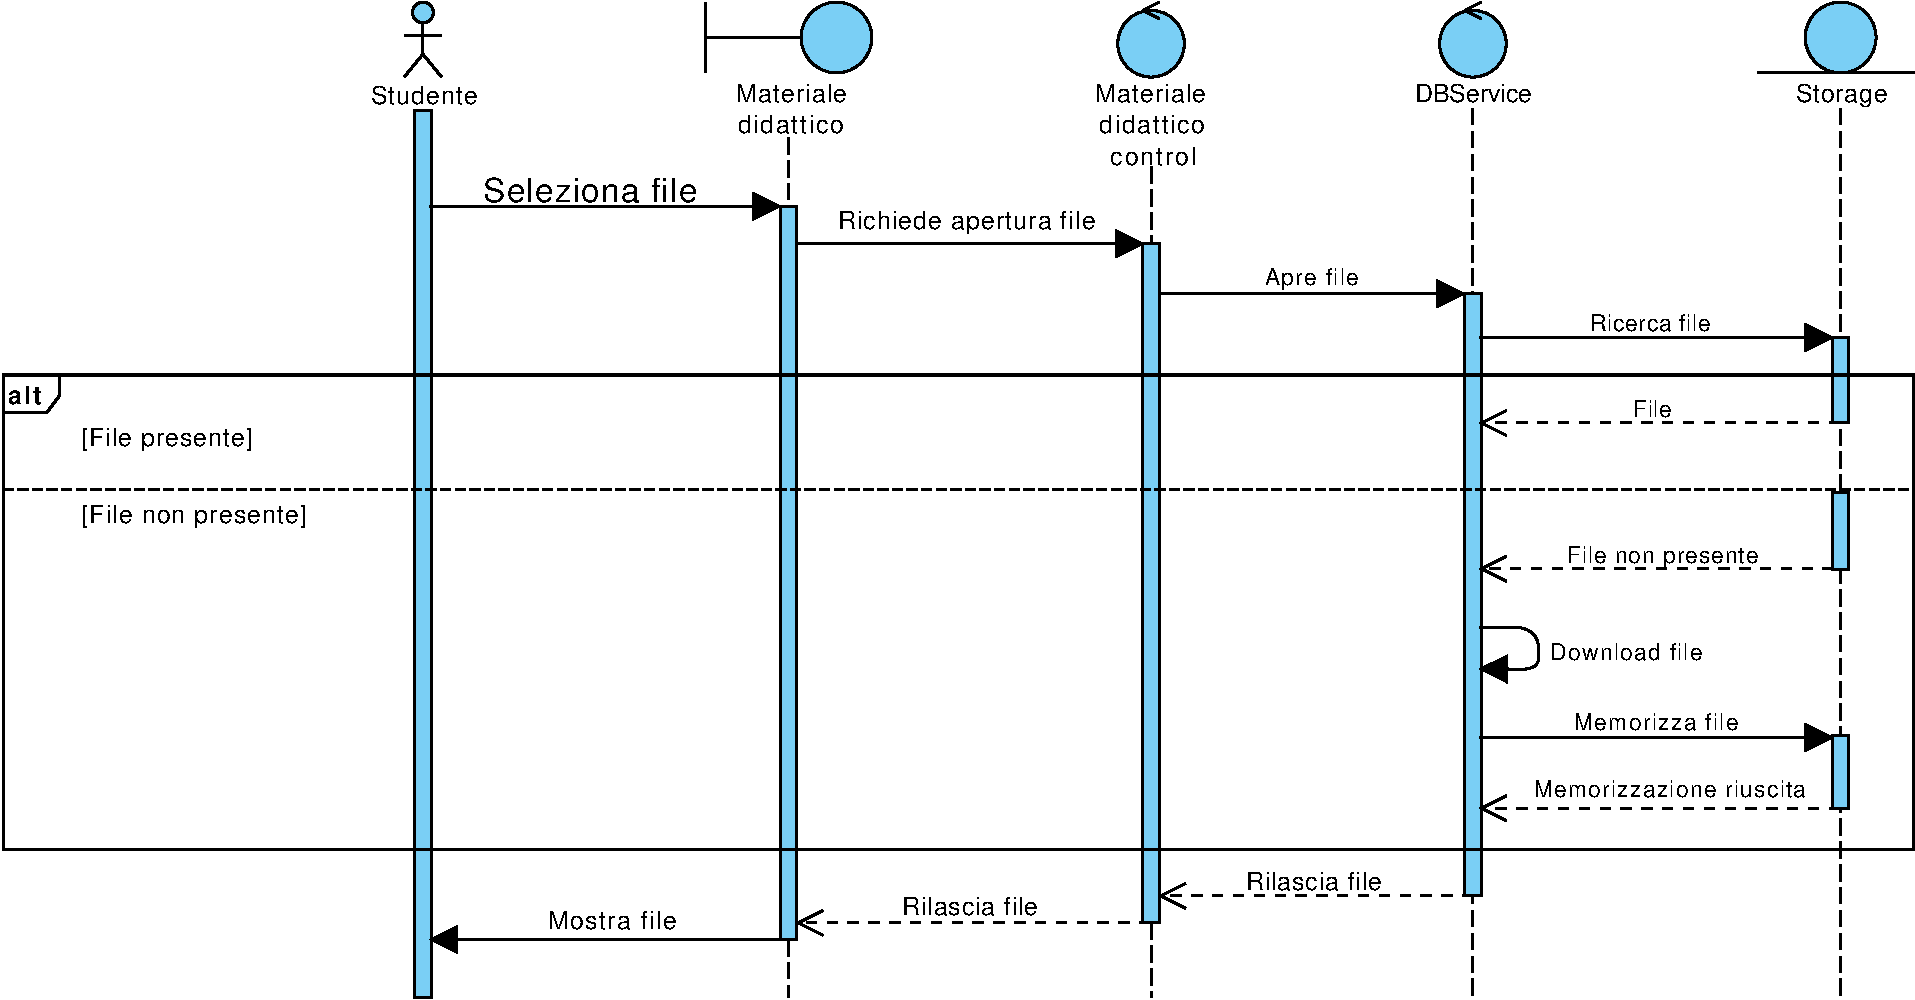
\includegraphics[width=6.5in]{imgs/gruppo1/sequence_diagrams/SD16_apri_file.pdf}
	\caption{Sequence Diagram - Apri file}
	\label{diag:apriFileSD}
\end{figure}
\newpage

%\paragraph{Rimuovi  file}
\begin{figure}
	\centering
	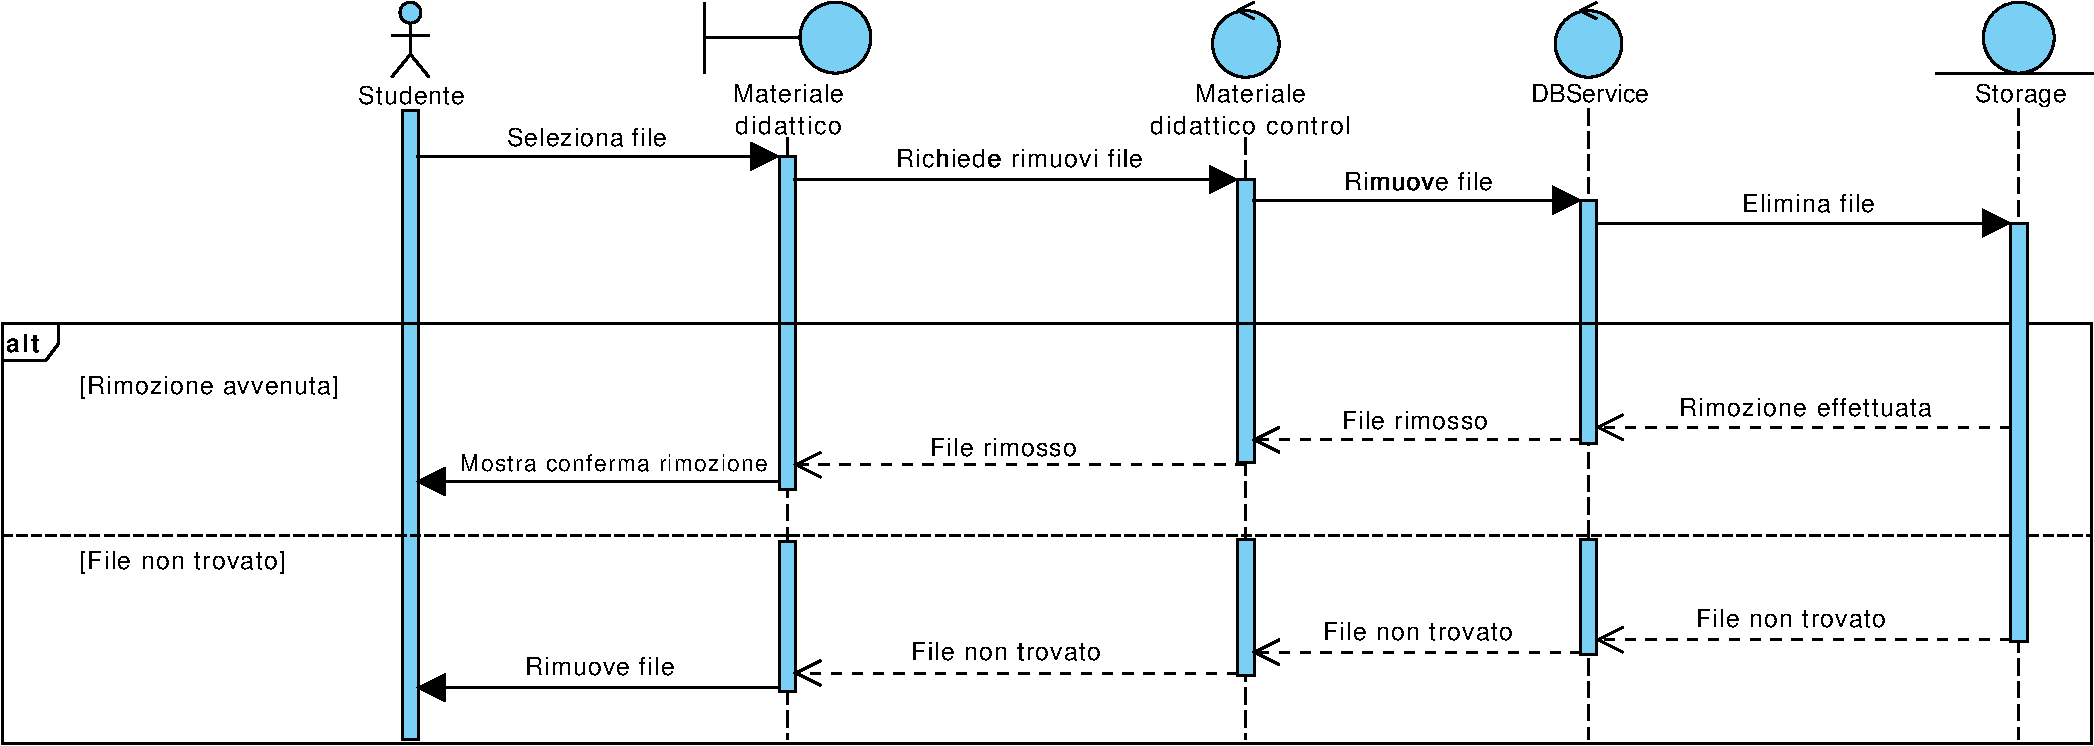
\includegraphics[width=6.5in]{imgs/gruppo1/sequence_diagrams/SD17_rimuovi_file.pdf}
	\caption{Sequence Diagram - Rimuovi file}
	\label{diag:rimuoviFileSD}
\end{figure}

\clearpage
\subsection{Funzionalità orario}

\subsubsection{Gestione primo avvio}

Giulio, dopo aver selezionato la sezione “orario” dalla voce del menu, potrà spuntare, da una lista di corsi, quelli che vuole seguire. Confermerà la selezione premendo l’apposito tasto “OK”. Da questo momento in poi Giulio potrà visualizzare l’orario costituito dai corsi scelti. 

\subsubsection{Modifica orario}

Giulio modificherà l’orario del proprio anno accademico spuntando la lista dei corsi che vuole seguire. Una volta confermata la modifica, lo studente visualizzerà l’orario aggiornato. 

\subsubsection{Visualizza orario}

Dopo il primo avvio dell’orario, selezionando la sezione “orario” dalla voce del menu, Giulio visualizzerà l’orario.
\subsection{Funzionalità notifiche}

Diagramma di sequenza: Vedi Figura~\vref{fig:seq-diagr-notifiche}.

\begin{figure}
	\centering
	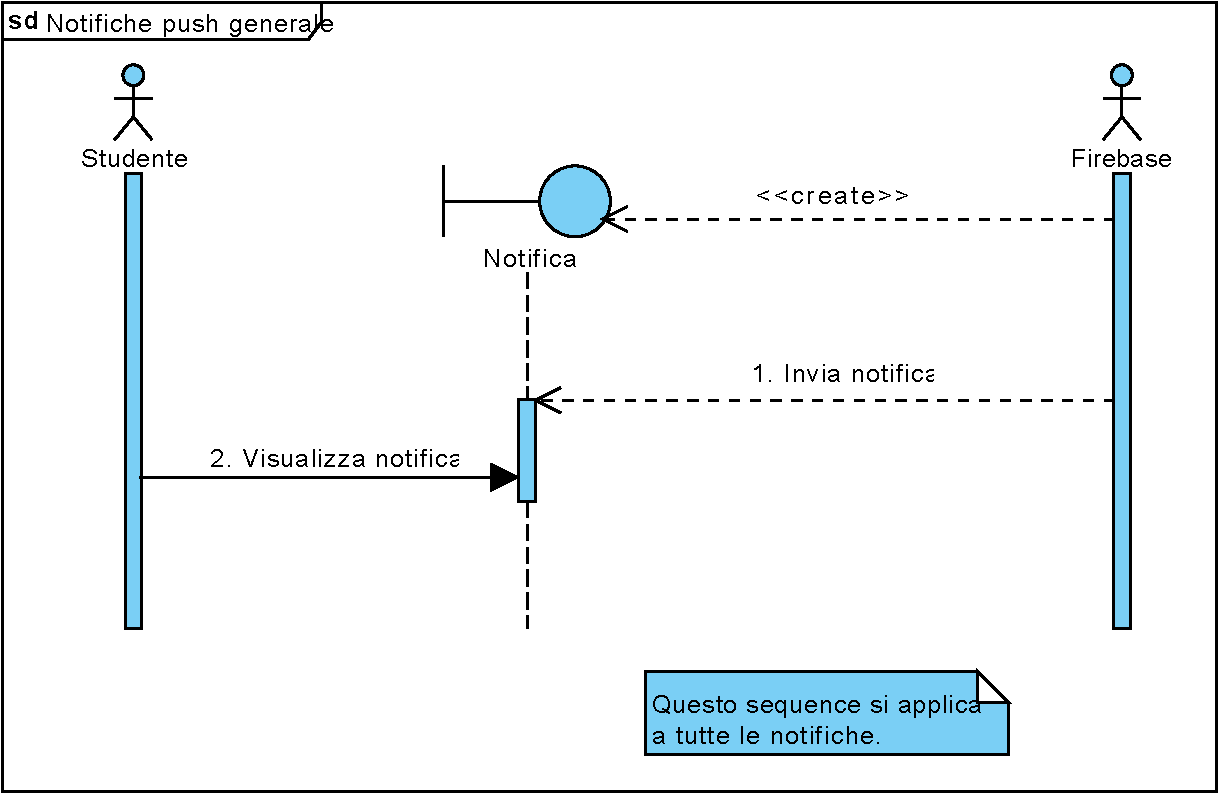
\includegraphics[width=0.85\textwidth]{imgs/gruppo2/sequence-notifiche}
	\caption{Sequence diagram - Notifiche}
	\label{fig:seq-diagr-notifiche}
\end{figure}

\clearpage
\subsection{Funzionalità chat}

\paragraph{CUS1 - Visualizza canale \\}

Lo \emph{Studente}, una volta selezionata la voce \emph{“chat”} dal \emph{menù} dell’app \emph{Studenti Unimol},  seleziona una \emph{chat} specifica della lista e visualizza i messaggi presenti nel canale di discussione della stessa. Nel caso in cui vi sia l’assenza di connessione viene visualizzata l’ultima copia salvata in locale del canale qualora essa sia presente.
\begin{table}
	\small % Dimensione testo piccola
	\label{CUS1 - Visualizza canale}
	\begin{tabular}{| p{\useCaseLeft} | p{\useCaseNum} | p{\useCaseTwoCol} | p{\useCaseTwoCol} |}
		\hline
		\textbf{Nome caso d'uso} & \multicolumn{3}{p{\useCaseMulticol} |}{\textbf{CUS 1 - Visualizza canale}} \\
		\hline
		\textbf{Attori partecipanti} & \multicolumn{3}{p{\useCaseMulticol} |}{Inizializzato da \textbf{\emph{Studente}.}} \\
		\hline
		\textbf{Condizioni d'ingresso} & \multicolumn{3}{p{\useCaseMulticol} |}{Lo \emph{Studente} seleziona la voce \emph{“chat”} dal \emph{menù} dell’\emph{app Studenti Unimol}.} \\
		\hline
		\textbf{Flusso degli eventi} & \textbf{\#} & \textbf{\emph{Studente}} & \textbf{Sistema} \\
		\hline
		\textbf{} & \textbf{1} & \textbf{} & Mostra l’\emph{home-chat} con le relative \emph{chat}; \\
		\hline
		\textbf{} & \textbf{2} & Seleziona la \emph{chat} desiderata; & \textbf{} \\
		\hline
		\textbf{} & \textbf{3} & \textbf{} & Mostra il canale di discussione di \emph{default} della \emph{chat}; \\
		\hline
		\textbf{} & \textbf{4} & Seleziona un canale di discussione alternativo; & \\
		\hline
		\textbf{} & \textbf{5} & \textbf{} & Mostra il canale di discussione selezionato; \\
		\hline
		\textbf{Eccezioni} & \multicolumn{3}{p{\useCaseMulticol} |}{1.1 - 3.1 - 5.1 Nessuna risposta dal \emph{server}: viene visualizzato un messaggio di errore; \newline1.2 - 3.2 - 5.2  Connessione assente: il sistema restituisce l’ultima copia salvata in locale; \newline 1.3 - 3.3 - 5.3 Copia non presente: viene visualizzato un messaggio di errore;} \\
		\hline
		\textbf{Condizioni d'uscita} & \multicolumn{3}{p{\useCaseMulticol} |}{Lo \emph{Studente} visualizza il canale correttamente.} \\
		\hline
	\end{tabular}
	\caption{CUS1 - Visualizza canale}
\end{table}

\newpage
	\paragraph{CUS2 - Invio messaggio \\}

Lo \emph{Studente}, all’interno di un canale di discussione, invia un messaggio selezionando l’apposito spazio dedito alla scrittura. Una volta digitato il testo del messaggio e selezionato il pulsante di invio, il sistema lo mostra nel canale di discussione. \\
\begin{table}

	\small % Dimensione testo piccola
	\label{CUS2 - Invio messaggio}
	\begin{tabular}{| p{\useCaseLeft} | p{\useCaseNum} | p{\useCaseTwoCol} | p{\useCaseTwoCol} |}
		\hline
		\textbf{Nome caso d'uso} & \multicolumn{3}{p{\useCaseMulticol} |}{\textbf{CUS2 - Invio messaggio}} \\
		\hline
		\textbf{Attori partecipanti} & \multicolumn{3}{p{\useCaseMulticol} |}{Inizializzato da \textbf{\emph{Studente}.}} \\
		\hline
		\textbf{Condizioni d'ingresso} & \multicolumn{3}{p{\useCaseMulticol} |}{Lo \emph{Studente} seleziona il canale di discussione in cui vuole inviare il messaggio.} \\
		\hline
		\textbf{Flusso degli eventi} & \textbf{\#} & \textbf{\emph{Studente}} & \textbf{Sistema} \\
		\hline
		\textbf{} & \textbf{1} & Seleziona la casella di testo, digita il messaggio ed invia; & \textbf{} \\
		\hline
		\textbf{} & \textbf{2} & \textbf{} & Riceve il messaggio e lo mostra nella \emph{chat}; \\
		\hline
		\textbf{Eccezioni} & \multicolumn{3}{p{\useCaseMulticol} |}{1.1 Connessione assente: il messaggio viene messo in coda e inviato quando sarà disponibile la connessione; \newline2.1 Nessuna risposta dal \emph{server}: viene visualizzato un messaggio di errore;} \\
		\hline
		\textbf{Condizioni d'uscita} & \multicolumn{3}{p{\useCaseMulticol} |}{Lo \emph{Studente} visualizza il messaggio nel canale della \emph{chat}.} \\
		\hline
	\end{tabular}
	\caption{CUS2 - Invio messaggio}
\end{table}


\newpage
\paragraph{CUS3 - Invio allegato \\}

Lo \emph{Studente} invia un file che viene mostrato all’interno del canale di discussione, similmente ad un messaggio. \\
	
\begin{table}
	
	\small % Dimensione testo piccola
	\label{CUS3 - Invio allegato}	
	\begin{tabular}{| p{\useCaseLeft} | p{\useCaseNum} | p{\useCaseTwoCol} | p{\useCaseTwoCol} |}
		\hline
		\textbf{Nome caso d'uso} & \multicolumn{3}{p{\useCaseMulticol} |}{\textbf{CUS3 - Invio Allegato}} \\
		\hline
		\textbf{Attori partecipanti} & \multicolumn{3}{p{\useCaseMulticol} |}{Inizializzato da \textbf{\emph{Studente}.}} \\
		\hline
		\textbf{Condizioni d'ingresso} & \multicolumn{3}{p{\useCaseMulticol} |}{Lo \emph{Studente} seleziona un canale di discussione.} \\
		\hline
		\textbf{Flusso degli eventi} & \textbf{\#} & \textbf{\emph{Studente}} & \textbf{Sistema} \\
		\hline
		\textbf{} & \textbf{1} & Seleziona il pulsante di scelta allegato; & \textbf{} \\
		\hline
		\textbf{} & \textbf{2} & \textbf{} & Mostra l’elenco dei \emph{file} presenti sul dispositivo dell’utente; \\
		\hline
		\textbf{} & \textbf{3} & Seleziona il \emph{file} da allegare; & \textbf{} \\
		\hline
		\textbf{} & \textbf{4} & \textbf{} & Controlla se l’allegato è idoneo all’invio nel canale di comunicazione e mostra un messaggio di conferma; \\
		\hline
		\textbf{} & \textbf{5} & Invia l’allegato; & \textbf{} \\
		\hline
		\textbf{} & \textbf{6} & \textbf{} & Conferma l’invio dell’allegato; \\
		\hline
		\textbf{Eccezioni} & \multicolumn{3}{p{\useCaseMulticol} |}{2.1 - 4.1 Nessuna risposta dal \emph{server}: viene visualizzato un messaggio di errore; \newline 3.1 Il \emph{file} non è idoneo: viene visualizzato un messaggio di errore; \newline 4.2 Connessione assente: l’allegato viene messo in coda e inviato quando sarà disponibile la connessione;} \\
		\hline
		\textbf{Condizioni d'uscita} & \multicolumn{3}{p{\useCaseMulticol} |}{Il sistema mostra l’allegato nel canale di comunicazione.} \\
		\hline
	\end{tabular}
	\caption{CUS3 - Invio allegato}
\end{table}


\newpage
\paragraph{CUS4 - Rispondi a singolo messaggio \\}
Lo \emph{Studente} visualizza il canale di discussione  desiderato e seleziona il singolo messaggio a cui desidera rispondere. \\
\begin{table}
	\small % Dimensione testo piccola
	\label{CUS4 - Rispondi a singolo messaggio}
	\begin{tabular}{| p{\useCaseLeft} | p{\useCaseNum} | p{\useCaseTwoCol} | p{\useCaseTwoCol} |}
		\hline
		\textbf{Nome caso d'uso} & \multicolumn{3}{p{\useCaseMulticol} |}{\textbf{CUS4 - Rispondi a singolo messaggio}} \\
		\hline
		\textbf{Attori partecipanti} & \multicolumn{3}{p{\useCaseMulticol} |}{Inizializzato da \textbf{\emph{Studente}.}} \\
		\hline
		\textbf{Condizioni d'ingresso} & \multicolumn{3}{p{\useCaseMulticol} |}{Lo \emph{Studente} seleziona il canale di discussione che contiene il messaggio a cui vuole rispondere.} \\
		\hline
		\textbf{Flusso degli eventi} & \textbf{\#} & \textbf{\emph{Studente}} & \textbf{Sistema} \\
		\hline
		\textbf{} & \textbf{1} & Seleziona un messaggio; & \textbf{} \\
		\hline
		\textbf{} & \textbf{2} & \textbf{} & Mostra il \emph{menú}; \\
		\hline
		\textbf{} & \textbf{3} & Seleziona l’opzione di risposta a messaggio; & \textbf{} \\
		\hline
		\textbf{} & \textbf{4} & \textbf{} & Evidenzia il messaggio a cui si vuole rispondere; \\
		\hline
		\textbf{Eccezioni} & \multicolumn{3}{p{\useCaseMulticol} |}{ \textbf{} } \\
		\hline
		\textbf{Condizioni d'uscita} & \multicolumn{3}{p{\useCaseMulticol} |}{Lo \emph{Studente} visualizza il messaggio evidenziato.} \\
		\hline
	\end{tabular}
	\caption{CUS4 - Rispondi a singolo messaggio}
\end{table}


\newpage
\paragraph{CUS5 - Scarica allegato \\}
Lo \emph{Studente} è intenzionato a scaricare un \emph{file} presente nel canale di discussione. \\
\begin{table}
	\small % Dimensione testo piccola
	\label{CUS5 - Scarica allegato}
	
	\begin{tabular}{| p{\useCaseLeft} | p{\useCaseNum} | p{\useCaseTwoCol} | p{\useCaseTwoCol} |}
		\hline
		\textbf{Nome caso d'uso} & \multicolumn{3}{p{\useCaseMulticol} |}{\textbf{CUS5 - Scarica allegato}} \\
		\hline
		\textbf{Attori partecipanti} & \multicolumn{3}{p{\useCaseMulticol} |}{Inizializzato da \textbf{\emph{Studente}.}} \\
		\hline
		\textbf{Condizioni d'ingresso} & \multicolumn{3}{p{\useCaseMulticol} |}{Lo \emph{Studente} seleziona un canale di discussione.} \\
		\hline
		\textbf{Flusso degli eventi} & \textbf{\#} & \textbf{\emph{Studente}} & \textbf{Sistema} \\
		\hline
		\textbf{} & \textbf{1} & Selezione il messaggio dove è presente l’allegato; & \textbf{} \\
		\hline
		\textbf{} & \textbf{2} & \textbf{} & Mostra l’opzione di scaricare l’allegato associato al messaggio selezionato; \\
		\hline
		\textbf{} & \textbf{3} & Seleziona l’opzione per scaricare l’allegato; & \textbf{} \\
		\hline
		\textbf{Eccezioni} & \multicolumn{3}{p{\useCaseMulticol} |}{1.1  Connessione assente: viene visualizzato un messaggio di errore; \newline3.1 Lo \emph{Studente} nega il \emph{download} dell’allegato: l’allegato non viene salvato sul dispositivo;} \\
		\hline
		\textbf{Condizioni d'uscita} & \multicolumn{3}{p{\useCaseMulticol} |}{Il sistema salva il file sul dispositivo.} \\
		\hline
	\end{tabular}
	\caption{CUS5 - Scarica allegato}
\end{table}


\newpage
\paragraph{CUS6 - Segnalazione messaggio \\}
Lo \emph{Studente} dopo aver visualizzato la chat interessata seleziona il messaggio che desidera segnalare. \\
\begin{table}
	\small % Dimensione testo piccola
	\label{CUS6 - Segnalazione messaggio}
	
	\begin{tabular}{| p{\useCaseLeft} | p{\useCaseNum} | p{\useCaseTwoCol} | p{\useCaseTwoCol} |}
		\hline
		\textbf{Nome caso d'uso} & \multicolumn{3}{p{\useCaseMulticol} |}{\textbf{CUS6 - Segnalazione messaggio}} \\
		\hline
		\textbf{Attori partecipanti} & \multicolumn{3}{p{\useCaseMulticol} |}{Inizializzato da \textbf{\emph{Studente}.}} \\
		\hline
		\textbf{Condizioni d'ingresso} & \multicolumn{3}{p{\useCaseMulticol} |}{Lo \emph{Studente} seleziona il canale di discussione che contiene il messaggio che vuole segnalare.} \\
		\hline
		\textbf{Flusso degli eventi} & \textbf{\#} & \textbf{\emph{Studente}} & \textbf{Sistema} \\
		\hline
		\textbf{} & \textbf{1} & Seleziona un messaggio; & \textbf{} \\
		\hline
		\textbf{} & \textbf{2} & \textbf{} & Mostra il \emph{menú}; \\
		\hline
		\textbf{} & \textbf{3} & Seleziona l’opzione “Segnala”; & \textbf{} \\
		\hline
		\textbf{} & \textbf{4} & \textbf{} & Chiede conferma di invio segnalazione; \\
		\hline
		\textbf{} & \textbf{5} & Conferma invio segnalazione; & \textbf{} \\
		\hline
		\textbf{} & \textbf{6} & \textbf{} & Conferma l’avvenuta segnalazione;  \\
		\hline
		\textbf{Eccezioni} & \multicolumn{3}{p{\useCaseMulticol} |}{3.1 Connessione assente: viene visualizzato un messaggio di errore; \newline4.1 - 6.1 Nessuna risposta dal \emph{server}: verrà visualizzato un messaggio di errore;} \\
		\hline
		\textbf{Condizioni d'uscita} & \multicolumn{3}{p{\useCaseMulticol} |}{Il sistema conferma il successo dell’operazione.} \\
		\hline
	\end{tabular}
	\caption{CUS6 - Segnalazione messaggio}
\end{table}


\newpage
\paragraph{CUS7 - Ricerca testo nella chat \\}
Lo \emph{Studente} vuole visualizzare vecchi messaggi seleziona la voce “cerca” nel \emph{menù} interno del canale di discussione, digitando il testo da cercare in un’apposita casella di testo. Il sistema mostra tutti i messaggi che contengono il testo partendo dal più recente. \\
\begin{table}
	\small % Dimensione testo piccola
	\label{CUS7 - Ricerca testo nella chat}
	
	\begin{tabular}{| p{\useCaseLeft} | p{\useCaseNum} | p{\useCaseTwoCol} | p{\useCaseTwoCol} |}
		\hline
		\textbf{Nome caso d'uso} & \multicolumn{3}{p{\useCaseMulticol} |}{\textbf{CUS7 - Ricerca testo nella chat}} \\
		\hline
		\textbf{Attori partecipanti} & \multicolumn{3}{p{\useCaseMulticol} |}{Inizializzato da \textbf{\emph{Studente}.}} \\
		\hline
		\textbf{Condizioni d'ingresso} & \multicolumn{3}{p{\useCaseMulticol} |}{Lo \emph{Studente} seleziona un canale di discussione.} \\
		\hline
		\textbf{Flusso degli eventi} & \textbf{\#} & \textbf{\emph{Studente}} & \textbf{Sistema} \\
		\hline
		\textbf{} & \textbf{1} & Accede alla sezione \emph{“menù”} del canale di discussione; & \textbf{} \\
		\hline
		\textbf{} & \textbf{2} & \textbf{} & Mostra il \emph{menú}; \\
		\hline
		\textbf{} & \textbf{3} & Seleziona il pulsante di ricerca; & \textbf{} \\
		\hline
		\textbf{} & \textbf{4} & \textbf{} &  Mostra la casella di testo di ricerca; \\
		\hline
		\textbf{} & \textbf{5} & Digita il testo da cercare; & \textbf{} \\
		\hline
		\textbf{} & \textbf{6} & \textbf{} & Evidenzia il testo cercato nei messaggi, mostrando prima il più recente;\\
		\hline
		\textbf{} & \textbf{7} & Scorre i messaggi fino a trovare quello ricercato; & \textbf{} \\
		\hline
		\textbf{Eccezioni} & \multicolumn{3}{p{\useCaseMulticol} |}{2.1 - 4.1 - 6.1  Nessuna risposta dal \emph{server}: viene visualizzato un messaggio di errore; \newline6.2 Il testo cercato non è presente: viene visualizzato un messaggio di notifica;} \\
		\hline
		\textbf{Condizioni d'uscita} & \multicolumn{3}{p{\useCaseMulticol} |}{Il sistema evidenzia i messaggi che contengono il testo cercato.} \\
		\hline
	\end{tabular}
	\caption{CUS7 - Ricerca testo nella chat}
\end{table}


\newpage
\paragraph{CUS8 - Tag membro in messaggio \\}
Lo \emph{Studente} che si trova all’interno di un canale di discussione ha la possibilitá di richiamare l’attenzione di uno specifico membro durante la digitazione di un messaggio. Lo studente digita il nome del membro preceduto da un carattere speciale (@). Il membro selezionato viene avvisato tramite una notifica diretta. \\
\begin{table}
	\small % Dimensione testo piccola
	\label{CUS8 - Tag membro in messaggio}
	
	\begin{tabular}{| p{\useCaseLeft} | p{\useCaseNum} | p{\useCaseTwoCol} | p{\useCaseTwoCol} |}
		\hline
		\textbf{Nome caso d'uso} & \multicolumn{3}{p{\useCaseMulticol} |}{\textbf{CUS8 - Tag membro in messaggio}} \\
		\hline
		\textbf{Attori partecipanti} & \multicolumn{3}{p{\useCaseMulticol} |}{Inizializzato da \textbf{\emph{Studente}.}} \\
		\hline
		\textbf{Condizioni d'ingresso} & \multicolumn{3}{p{\useCaseMulticol} |}{Lo \emph{Studente} seleziona un canale di discussione.} \\
		\hline
		\textbf{Flusso degli eventi} & \textbf{\#} & \textbf{\emph{Studente}} & \textbf{Sistema} \\
		\hline
		\textbf{} & \textbf{1} & Seleziona la  casella di testo quindi digita il nome di un membro preceduto dal carattere speciale; & \textbf{} \\
		\hline
		\textbf{} & \textbf{2} & \textbf{} & Mostra la lista di utenti che corrispondono al nome inserito; \\
		\hline
		\textbf{} & \textbf{3} & Seleziona il membro da taggare; & \textbf{} \\
		\hline
		\textbf{Eccezioni} & \multicolumn{3}{p{\useCaseMulticol} |}{1.1 Lo  \emph{Studente} digita il nome errato: il testo digitato viene inserito come messaggio di testo;} \\
		\hline
		\textbf{Condizioni d'uscita} & \multicolumn{3}{p{\useCaseMulticol} |}{Il sistema mostra il messaggio contenente il  \emph{tag} all’interno della casella di testo.} \\
		\hline
	\end{tabular}
	\caption{CUS8 - Tag membro in messaggio}
\end{table}


\newpage
\paragraph{CUS9 - Gestisci notifiche chat \\}
Lo \emph{Studente} che si trova all’interno di una \emph{chat} ha la possibilitá di accedere al \emph{menù} e gestire le notifiche ovvero di attivarle o disattivarle in base alle sue preferenze. \\
\begin{table}
	\small % Dimensione testo piccola
	\label{CUS9 - Gestisci notifiche chat}
	
	\begin{tabular}{| p{\useCaseLeft} | p{\useCaseNum} | p{\useCaseTwoCol} | p{\useCaseTwoCol} |}
		\hline
		\textbf{Nome caso d'uso} & \multicolumn{3}{p{\useCaseMulticol} |}{\textbf{CUS9 - Gestisci notifiche chat}} \\
		\hline
		\textbf{Attori partecipanti} & \multicolumn{3}{p{\useCaseMulticol} |}{Inizializzato da \textbf{\emph{Studente}.}} \\
		\hline
		\textbf{Condizioni d'ingresso} & \multicolumn{3}{p{\useCaseMulticol} |}{Lo \emph{Studente} seleziona un canale di discussione.} \\
		\hline
		\textbf{Flusso degli eventi} & \textbf{\#} & \textbf{\emph{Studente}} & \textbf{Sistema} \\
		\hline
		\textbf{} & \textbf{1} & Accede alla sezione \emph{menú} del canale di discussione; & \textbf{} \\
		\hline
		\textbf{} & \textbf{2} & \textbf{} & Mostra il \emph{menú}; \\
		\hline
		\textbf{} & \textbf{3} & Seleziona il pulsante per attivare/disattivare le notifiche della \emph{chat}; & \textbf{} \\
		\hline
		\textbf{Eccezioni} & \multicolumn{3}{p{\useCaseMulticol} |}{3.1  Connessione assente: viene visualizzato un messaggio di errore; \newline 3.2  Nessuna risposta dal \emph{server}: viene visualizzato un messaggio di errore;} \\
		\hline
		\textbf{Condizioni d'uscita} & \multicolumn{3}{p{\useCaseMulticol} |}{Il sistema cambia lo stato delle notifiche della \emph{chat}.} \\
		\hline
	\end{tabular}
	\caption{CUS9 - Gestisci notifiche chat}
\end{table}


\newpage
\paragraph{CUS10 - Selezione \emph{emoji} \\}
Lo \emph{Studente} che si trova all’interno di un canale di discussione ha la possibilitá di scegliere una o piú \emph{emoji} tra quelle disponibili. \\
\begin{table}
	\small % Dimensione testo piccola
	\label{CUS10 - Selezione emoji}
	
	\begin{tabular}{| p{\useCaseLeft} | p{\useCaseNum} | p{\useCaseTwoCol} | p{\useCaseTwoCol} |}
		\hline
		\textbf{Nome caso d'uso} & \multicolumn{3}{p{\useCaseMulticol} |}{\textbf{CUS10 - Selezione \emph{emoji}}} \\
		\hline
		\textbf{Attori partecipanti} & \multicolumn{3}{p{\useCaseMulticol} |}{Inizializzato da \textbf{\emph{Studente}.}} \\
		\hline
		\textbf{Condizioni d'ingresso} & \multicolumn{3}{p{\useCaseMulticol} |}{Lo \emph{Studente} seleziona un canale di discussione.} \\
		\hline
		\textbf{Flusso degli eventi} & \textbf{\#} & \textbf{\emph{Studente}} & \textbf{Sistema} \\
		\hline
		\textbf{} & \textbf{1} & Seleziona l’icona \emph{emoji}; & \textbf{} \\
		\hline
		\textbf{} & \textbf{2} & \textbf{} & Mostra una finestra con le \emph{emoji} disponibili; \\
		\hline
		\textbf{} & \textbf{3} & Seleziona una o piú \emph{emoji}; & \textbf{} \\
		\hline
		\textbf{} & \textbf{4} & \textbf{} & Il sistema inserisce l’\emph{emoji} nel messaggio; \\
		\hline
		\textbf{Eccezioni} & \multicolumn{3}{p{\useCaseMulticol} |}{ \textbf{} } \\
		\hline
		\textbf{Condizioni d'uscita} & \multicolumn{3}{p{\useCaseMulticol} |}{Lo \emph{Studente} visualizza il messaggio contenente le \emph{emoji} selezionate.} \\
		\hline
	\end{tabular}
	\caption{CUS10 - Selezione \emph{emoji}}
\end{table}


\newpage
\paragraph{CUS11 - Visualizza elenco membri chat \\}
Lo \emph{Studente} visualizza il numero dei partecipanti al canale di discussione e l’elenco contenente l’\emph{username} degli stessi. Nel caso in cui vi sia l’assenza di connessione viene visualizzata l’ultima copia salvata in locale dell’elenco dei partecipanti al canale qualora essa sia presente. \\
\begin{table}
	\small % Dimensione testo piccola
	\label{CUS11 - Visualizza elenco membri chat}
	
	\begin{tabular}{| p{\useCaseLeft} | p{\useCaseNum} | p{\useCaseTwoCol} | p{\useCaseTwoCol} |}
		\hline
		\textbf{Nome caso d'uso} & \multicolumn{3}{p{\useCaseMulticol} |}{\textbf{CUS11 - Visualizza elenco membri chat}} \\
		\hline
		\textbf{Attori partecipanti} & \multicolumn{3}{p{\useCaseMulticol} |}{Inizializzato da \textbf{\emph{Studente}.}} \\
		\hline
		\textbf{Condizioni d'ingresso} & \multicolumn{3}{p{\useCaseMulticol} |}{Lo \emph{Studente} seleziona un canale di discussione.} \\
		\hline
		\textbf{Flusso degli eventi} & \textbf{\#} & \textbf{\emph{Studente}} & \textbf{Sistema} \\
		\hline
		\textbf{} & \textbf{1} & Seleziona il nome del canale di discussione; & \textbf{} \\
		\hline
		\textbf{} & \textbf{2} & \textbf{} & Mostra il numero dei membri del canale di discussione e l’elenco dei loro nomi; \\
		\hline
		\textbf{Eccezioni} & \multicolumn{3}{p{\useCaseMulticol} |}{2.1 Nessuna risposta dal \emph{server}: viene visualizzato un messaggio di errore; \newline2.2 Connessione assente: il sistema restituisce l’ultima copia salvata in locale; \newline2.3 Copia non presente: viene visualizzato un messaggio di errore;} \\
		\hline
		\textbf{Condizioni d'uscita} & \multicolumn{3}{p{\useCaseMulticol} |}{Lo \emph{Studente} visualizza l’elenco dei membri del canale di discussione.} \\
		\hline
	\end{tabular}
	\caption{CUS11 - Visualizza elenco membri chat}
\end{table}

\paragraph{CUE1 - Connessione assente \\}
Lo \emph{Studente} effettua un’operazione che richiede connessione alla rete ma quest’ultima non è disponibile pertanto visualizza un messaggio d’errore. \\
\begin{table}
	\small % Dimensione testo piccola
	\label{CUE1 - Connessione assente}
	\begin{tabular}{| p{\useCaseLeft} | p{\useCaseNum} | p{\useCaseTwoCol} | p{\useCaseTwoCol} |}
		\hline
		\textbf{Nome caso d'uso} & \multicolumn{3}{p{\useCaseMulticol} |}{\textbf{CUE1 - Connessione assente}} \\
		\hline
		\textbf{Attori partecipanti} & \multicolumn{3}{p{\useCaseMulticol} |}{Inizializzato da \textbf{Sistema}, partecipa \textbf{\emph{Studente}.}} \\
		\hline
		\textbf{Condizioni d'ingresso} & \multicolumn{3}{p{\useCaseMulticol} |}{Lo \emph{Studente} effettua un’operazione che richiede connessione alla rete.} \\
		\hline
		\textbf{Flusso degli eventi} & \textbf{\#} & \textbf{\emph{Studente}} & \textbf{Sistema} \\
		\hline
		\textbf{} & \textbf{1} & \textbf{} & Mostra un messaggio d’errore; \\
		\hline
		\textbf{Eccezioni} & \multicolumn{3}{p{\useCaseMulticol} |}{ \textbf{} } \\
		\hline
		\textbf{Condizioni d'uscita} & \multicolumn{3}{p{\useCaseMulticol} |}{Lo \emph{Studente} visualizza il messaggio d’errore.} \\
		\hline
	\end{tabular}
	\caption{CUE1 - Connessione assente}
\end{table}


\newpage
\paragraph{CUE2 - Nessuna risposta dal sistema \\}
Lo \emph{Studente} effettua un’operazione che richiede una risposta dal Sistema, ma quest’ultimo non è in grado di soddisfare la richiesta pertanto visualizza un messaggio d’errore. \\
\begin{table}
	\small % Dimensione testo piccola
	\label{CUE2 - Nessuna risposta dal sistema}
	
	
	Lo \emph{Studente} effettua un’operazione che richiede una risposta dal Sistema, ma quest’ultimo non è in grado di soddisfare la richiesta pertanto visualizza un messaggio d’errore. \\
	
	\begin{tabular}{| p{\useCaseLeft} | p{\useCaseNum} | p{\useCaseTwoCol} | p{\useCaseTwoCol} |}
		\hline
		\textbf{Nome caso d'uso} & \multicolumn{3}{p{\useCaseMulticol} |}{\textbf{CUE2 - Nessuna risposta dal sistema}} \\
		\hline
		\textbf{Attori partecipanti} & \multicolumn{3}{p{\useCaseMulticol} |}{Inizializzato da \textbf{Sistema}, partecipa \textbf{\emph{Studente}.}} \\
		\hline
		\textbf{Condizioni d'ingresso} & \multicolumn{3}{p{\useCaseMulticol} |}{Il Sistema riceve un messaggio di errore.} \\
		\hline
		\textbf{Flusso degli eventi} & \textbf{\#} & \textbf{\emph{Studente}} & \textbf{Sistema} \\
		\hline
		\textbf{} & \textbf{1} & \textbf{} & Riscontra un errore e lo inoltra allo \emph{Studente}; \\
		\hline
		\textbf{Eccezioni} & \multicolumn{3}{p{\useCaseMulticol} |}{ \textbf{} } \\
		\hline
		\textbf{Condizioni d'uscita} & \multicolumn{3}{p{\useCaseMulticol} |}{Lo \emph{Studente} visualizza il messaggio d’errore.} \\
		\hline
	\end{tabular}
	\caption{CUE2 - Nessuna risposta dal sistema}
\end{table}

\paragraph{CUD1 - Creazione canale \\}
Il \emph{Docente}, che si trova all'interno di un cnale di discussione accede alla sezione "\emph{menù}" e crea un nuovo canale all'interno di quello attuale in uso, assengando ad esso un nome ed aggiungendo uno o più membri. \\
\begin{table}
	\small % Dimensione testo piccola
	\label{CUD1 - Creazione canale}
	\begin{tabular}{| p{\useCaseLeft} | p{\useCaseNum} | p{\useCaseTwoCol} | p{\useCaseTwoCol} |}
		\hline
		\textbf{Nome caso d'uso} & \multicolumn{3}{p{\useCaseMulticol} |}{\textbf{CUD1 - Creazione canale}} \\
		\hline
		\textbf{Attori partecipanti} & \multicolumn{3}{p{\useCaseMulticol} |}{Inizializzato da \textbf{\emph{Docente}.}} \\ 
		\hline
		\textbf{Condizioni d'ingresso} & \multicolumn{3}{p{\useCaseMulticol} |}{Il \emph{Docente} seleziona un canale di discussione.} \\
		\hline
		\textbf{Flusso degli eventi} & \textbf{\#} & \textbf{\emph{Docente}} & \textbf{Sistema} \\
		\hline
		\textbf{} & \textbf{1} & Accede alla sezione \emph{menù} del canale di discussione; & \textbf{} \\
		\hline
		\textbf{} & \textbf{2} & \textbf{} & Mostra il \emph{menù}; \\
		\hline
		\textbf{} & \textbf{3} & Seleziona la voce di creazione del nuovo canale; & \textbf{} \\
		\hline
		\textbf{} & \textbf{4} & \textbf{} & Chiede l'immissione del nome del nuovo canale; \\
		\hline
		\textbf{} & \textbf{5} & Inserisce il nome del nuovo canale; & \textbf{} \\
		\hline
		\textbf{} & \textbf{6} & \textbf{} & Chiede conferma del nome inserito; \\
		\hline
		\textbf{} & \textbf{7} & Conferma il nome inserito; & \textbf{} \\
		\hline
		\textbf{} & \textbf{8} & \textbf{} & Chiede l'identificativo dei membri da inserire all'interno del canale; \\
		\hline
		\textbf{} & \textbf{9} & Inserisce l'identificativo dei membri da aggiungere al canale; & \textbf{} \\
		\hline
		\textbf{} & \textbf{10} & \textbf{} & Chiede conferma degli identificativi inseriti; \\
		\hline
		\textbf{} & \textbf{11} & Conferma gli identificativi inseriti; & \textbf{} \\
		\hline
		\textbf{} & \textbf{10} & \textbf{} & Conferma la creazione del canale; \\
		\hline
		\textbf{Eccezioni} & \multicolumn{3}{p{\useCaseMulticol} |}{3.1 Connessione assente: il sistema non procede con la creazione canale; \newline 4.1 - 6.1 - 8.1 - 10.1 - 12.1 Nessuna risposta dal \emph{server}: viene visualizzato un messaggio di errore;} \\
		\hline
		\textbf{Condizioni d'uscita} & \multicolumn{3}{p{\useCaseMulticol} |}{Il \emph{Docente} visualizza il canale appena creato.} \\
		\hline
	\end{tabular}
	\caption{CUD1 - Creazione canale}
\end{table}


\newpage
\paragraph{CUD2 - Cancellazione canale \\}
Il \emph{Docente} che si trova all'interno di un canale di discussione accede alla sezione "\emph{menù}" e effettua la cancellazione di uno dei canali presenti all'interno della \emph{chat}. \\
\begin{table}
	\small % Dimensione testo piccola
	\label{CUD2 - Cancellazione canale}
	\begin{tabular}{| p{\useCaseLeft} | p{\useCaseNum} | p{\useCaseTwoCol} | p{\useCaseTwoCol} |}
		\hline
		\textbf{Nome caso d'uso} & \multicolumn{3}{p{\useCaseMulticol} |}{\textbf{CUD2 - Cancellazione canale}} \\
		\hline
		\textbf{Attori partecipanti} & \multicolumn{3}{p{\useCaseMulticol} |}{Inizializzato da \textbf{\emph{Docente}.}} \\ 
		\hline
		\textbf{Condizioni d'ingresso} & \multicolumn{3}{p{\useCaseMulticol} |}{Il \emph{Docente} seleziona un canale di discussione.} \\
		\hline
		\textbf{Flusso degli eventi} & \textbf{\#} & \textbf{\emph{Docente}} & \textbf{Sistema} \\
		\hline
		\textbf{} & \textbf{1} & Accede alla sezione \emph{menù} del canale di discussione; & \textbf{} \\
		\hline
		\textbf{} & \textbf{2} & \textbf{} & Mostra il \emph{menù}; \\
		\hline
		\textbf{} & \textbf{3} & Seleziona la voce di cancellazione del canale; & \textbf{} \\
		\hline
		\textbf{} & \textbf{4} & \textbf{} & Chiede conferma della cancellaizone; \\
		\hline
		\textbf{} & \textbf{5} & Conferma la scelta; & \textbf{} \\
		\hline
		\textbf{} & \textbf{6} & \textbf{} & procede alla cancellazione del canale; \\
		\hline
		\textbf{Eccezioni} & \multicolumn{3}{p{\useCaseMulticol} |}{3.1 Connessione assente: il canale non viene cancellato; \newline E' presente un solo canale di discussione: il canale non viene cancellato; \newline 4.1 - 6.1 Nessuna risposta dal \emph{server}: viene visualizzato un messaggio di errore;} \\
		\hline
		\textbf{Condizioni d'uscita} & \multicolumn{3}{p{\useCaseMulticol} |}{Il \emph{Docente} visualizza i canali attivi.} \\
		\hline
	\end{tabular}
	\caption{CUD2 - Cancellazione canale}
\end{table}


\newpage
\paragraph{CUD3 - Aggiungi membro ad un canale \\}
Il \emph{Docente} che si trova all'interno di un canale di discussione ha la possibilità di aggiungere un nuovo membro ad un canale attraverso il \emph{menù} di modifica che include l'opzione di aggiunta nuovo membro. \\
\begin{table}
	\small % Dimensione testo piccola
	\label{CUD3 - Aggiungi membro ad un canale}
		\begin{tabular}{| p{\useCaseLeft} | p{\useCaseNum} | p{\useCaseTwoCol} | p{\useCaseTwoCol} |}
		\hline
		\textbf{Nome caso d'uso} & \multicolumn{3}{p{\useCaseMulticol} |}{\textbf{CUD3 - Aggiungi membro ad un canale}} \\
		\hline
		\textbf{Attori partecipanti} & \multicolumn{3}{p{\useCaseMulticol} |}{Inizializzato da \textbf{\emph{Docente}.}} \\ 
		\hline
		\textbf{Condizioni d'ingresso} & \multicolumn{3}{p{\useCaseMulticol} |}{Il \emph{Docente} seleziona un canale di discussione.} \\
		\hline
		\textbf{Flusso degli eventi} & \textbf{\#} & \textbf{\emph{Docente}} & \textbf{Sistema} \\
		\hline
		\textbf{} & \textbf{1} & Accede alla sezione \emph{menù} del canale di discussione; & \textbf{} \\
		\hline
		\textbf{} & \textbf{2} & \textbf{} & Mostra il \emph{menù}; \\
		\hline
		\textbf{} & \textbf{3} & Seleziona la voce aggiungi nuovo membro al canale; & \textbf{} \\
		\hline
		\textbf{} & \textbf{4} & \textbf{} & Chiede l'identificativo del membro da aggiungere al canale; \\
		\hline
		\textbf{} & \textbf{5} & Inserisce l'identificativo del membro da aggiungere; & \textbf{} \\
		\hline
		\textbf{} & \textbf{6} & \textbf{} & Chiede conferma dell'identificativo inserito; \\
		\hline
		\textbf{} & \textbf{7} & Conferma i dati inseriti; & \textbf{} \\
		\hline
		\textbf{} & \textbf{8} & \textbf{} & Conferma l'aggiunta del nuovo \emph{Docente}; \\
		\hline
		\textbf{Eccezioni} & \multicolumn{3}{p{\useCaseMulticol} |}{3.1 Connessione assente: il membro non viene aggiunto; \newline 4.1 - 6.1 - 8.1 Nessuna risposta dal \emph{server}: viene visualizzato un messaggio di errore;} \\
		\hline
		\textbf{Condizioni d'uscita} & \multicolumn{3}{p{\useCaseMulticol} |}{Il \emph{Docente} visualizza l'elenco aggiornato dei membri assegnati al canale.} \\
		\hline
	\end{tabular}
	\caption{CUD3 - Aggiungi membro ad un canale}
\end{table}


\newpage
\paragraph{CUD4 - Rimuovi membro ad un canale \\}
Il \emph{Docente} che si trova all'interno di un canale di discussione ha la possibilità di rimuovere un \emph{Docente} o uno \emph{Studente} da un canale attraverso il \emph{menù} di modifica che include l'opzione di rimozione \emph{Docente} o \emph{Studente}. \\
\begin{table}
	\small % Dimensione testo piccola
	\label{CUD4 - Rimuovi membro ad un canale}
	\begin{tabular}{| p{\useCaseLeft} | p{\useCaseNum} | p{\useCaseTwoCol} | p{\useCaseTwoCol} |}
		\hline
		\textbf{Nome caso d'uso} & \multicolumn{3}{p{\useCaseMulticol} |}{\textbf{CUD4 - Rimuovi membro ad un canale}} \\
		\hline
		\textbf{Attori partecipanti} & \multicolumn{3}{p{\useCaseMulticol} |}{Inizializzato da \textbf{\emph{Docente}.}} \\ 
		\hline
		\textbf{Condizioni d'ingresso} & \multicolumn{3}{p{\useCaseMulticol} |}{Il \emph{Docente} seleziona un canale di discussione.} \\
		\hline
		\textbf{Flusso degli eventi} & \textbf{\#} & \textbf{\emph{Docente}} & \textbf{Sistema} \\
		\hline
		\textbf{} & \textbf{1} & Accede alla sezione \emph{menù} del canale di discussione; & \textbf{} \\
		\hline
		\textbf{} & \textbf{2} & \textbf{} & Mostra il \emph{menù}; \\
		\hline
		\textbf{} & \textbf{3} & Seleziona la voce rimuovi membro dal canale; & \textbf{} \\
		\hline
		\textbf{} & \textbf{4} & \textbf{} & Chiede l'immissione dell'identificativo del membro da rimuovere; \\
		\hline
		\textbf{} & \textbf{5} & Inserisce l'identificativo del membro; & \textbf{} \\
		\hline
		\textbf{} & \textbf{6} & \textbf{} & Chiede conferma dell'identificativo inserito; \\
		\hline
		\textbf{} & \textbf{7} & Conferma l'identificativo inserito; & \textbf{} \\
		\hline
		\textbf{} & \textbf{8} & \textbf{} & Conferma la rimozione del membro dal canale; \\
		\hline
		\textbf{Eccezioni} & \multicolumn{3}{p{\useCaseMulticol} |}{3.1 Connessione assente: non viene eliminato il membro dal canale; \newline 4.1 - 6.1 - 8.1 Nessuna risposta dal \emph{server}: viene visualizzato un messaggio di errore;} \\
		\hline
		\textbf{Condizioni d'uscita} & \multicolumn{3}{p{\useCaseMulticol} |}{Il \emph{Docente} visualizza l'elenco aggiornato dei membri assegnati al canale.} \\
		\hline
	\end{tabular}
	\caption{CUD4 - Rimuovi membro ad un canale}
\end{table}


\newpage
\paragraph{CUD5 - Blocca Studente \\}
Il \emph{Docente} ha la possibilità di silenziare uno \emph{Studente}, nel caso in cui ritenga inappropriati alcuni interventi nel canale di comunicazione. Per silenziare si intende impedire l'invio di nuovi messaggi ad un determinato \emph{Studente}. \\
\begin{table}
	\small % Dimensione testo piccola
	\label{CUD5 - Blocca Studente}
	\begin{tabular}{| p{\useCaseLeft} | p{\useCaseNum} | p{\useCaseTwoCol} | p{\useCaseTwoCol} |}
		\hline
		\textbf{Nome caso d'uso} & \multicolumn{3}{p{\useCaseMulticol} |}{\textbf{CUD5 - Blocca Studente}} \\
		\hline
		\textbf{Attori partecipanti} & \multicolumn{3}{p{\useCaseMulticol} |}{Inizializzato da \textbf{\emph{Docente}.}} \\ 
		\hline
		\textbf{Condizioni d'ingresso} & \multicolumn{3}{p{\useCaseMulticol} |}{Il \emph{Docente} seleziona un canale di discussione.} \\
		\hline
		\textbf{Flusso degli eventi} & \textbf{\#} & \textbf{\emph{Docente}} & \textbf{Sistema} \\
		\hline
		\textbf{} & \textbf{1} & Seleziona un messaggio; & \textbf{} \\
		\hline
		\textbf{} & \textbf{2} & \textbf{} & Mostra l'opzione di blocco dello \emph{Studente} associato al messaggio; \\
		\hline
		\textbf{} & \textbf{3} & Conferma il blocco dello \emph{Studente}; & \textbf{} \\
		\hline
		\textbf{} & \textbf{4} & \textbf{} & Blocca lo \emph{Studente} e mostra un messaggio di conferma; \\
		\hline
		\textbf{} & \textbf{1.1} & Seleziona il nome del canale di discussione; & \textbf{} \\
		\hline
		\textbf{} & \textbf{1.2} & \textbf{} & Mostra il numero dei membri della \emph{chat} e l'elenco dei loro nomi; \\
		\hline
		\textbf{} & \textbf{1.3} & Seleziona uno \emph{Studente}; & \textbf{} \\
		\hline
		\textbf{} & \textbf{2.1} & \textbf{} & Mostra l'opzione di blocco dello \emph{Studente}; \\
		\hline
		\textbf{Eccezioni} & \multicolumn{3}{p{\useCaseMulticol} |}{3.1 Il \emph{Docente} non conferma il blocco dello \emph{Studente}: lo \emph{Studente} non viene bloccato \newline Connessione assente: lo \emph{Studente} non viene bloccato; \newline 4.2 Nessuna risposta dal \emph{server}: viene visualizzato un messaggio di errore;} \\
		\hline
		\textbf{Condizioni d'uscita} & \multicolumn{3}{p{\useCaseMulticol} |}{Il sistema blocca lo \emph{Studente scelto}.} \\
		\hline
	\end{tabular}
	\caption{CUD5 - Blocca Studente}
\end{table}


\newpage
\paragraph{CUD6 - Sblocca Studente \\}
Il \emph{Docente} Il Docente ha la possibilità di sbloccare uno Studente precedentemente bloccato  nel caso in cui ritenga opportuno farlo, così da poter permettere nuovamente allo studente di inviare messaggi nel canale di discussione.    \\
\begin{table}
	\small % Dimensione testo piccola
	\label{CUD6 - Sblocca Studentee}
	\begin{tabular}{| p{\useCaseLeft} | p{\useCaseNum} | p{\useCaseTwoCol} | p{\useCaseTwoCol} |}
		\hline
		\textbf{Nome caso d'uso} & \multicolumn{3}{p{\useCaseMulticol} |}{\textbf{CUD6 - Sblocca Studente}} \\
		\hline
		\textbf{Attori partecipanti} & \multicolumn{3}{p{\useCaseMulticol} |}{Inizializzato da \textbf{\emph{Docente}.}} \\ 
		\hline
		\textbf{Condizioni d'ingresso} & \multicolumn{3}{p{\useCaseMulticol} |}{Il \emph{Docente} seleziona un canale di discussione.} \\
		\hline
		\textbf{Flusso degli eventi} & \textbf{\#} & \textbf{\emph{Docente}} & \textbf{Sistema} \\
		\hline
		\textbf{} & \textbf{1} & Seleziona un messaggio; & \textbf{} \\
		\hline
		\textbf{} & \textbf{2} & \textbf{} & Mostra l'opzione di sblocco dello \emph{Studente} associato al messaggio; \\
		\hline
		\textbf{} & \textbf{3} & Conferma lo sblocco dello \emph{Studente}; & \textbf{} \\
		\hline
		\textbf{} & \textbf{4} & \textbf{} & Sblocca lo \emph{Studente} e mostra un messaggio di conferma; \\
		\hline
		\textbf{} & \textbf{1.1} & Seleziona il nome del canale di discussione; & \textbf{} \\
		\hline
		\textbf{} & \textbf{1.2} & \textbf{} & Mostra il numero dei membri della \emph{chat} e l'elenco dei loro nomi; \\
		\hline
		\textbf{} & \textbf{1.3} & Seleziona uno \emph{Studente}; & \textbf{} \\
		\hline
		\textbf{} & \textbf{2.1} & \textbf{} & Mostra l'opzione di sblocco dello \emph{Studente}; \\
		\hline
		\textbf{Eccezioni} & \multicolumn{3}{p{\useCaseMulticol} |}{3.1 Il \emph{Docente} non conferma lo sblocco dello \emph{Studente}: lo \emph{Studente} non viene sbloccato \newline Connessione assente: lo \emph{Studente} non viene sbloccato; \newline 4.2 Nessuna risposta dal \emph{server}: viene visualizzato un messaggio di errore;} \\
		\hline
		\textbf{Condizioni d'uscita} & \multicolumn{3}{p{\useCaseMulticol} |}{Il sistema sblocca lo \emph{Studente scelto}.} \\
		\hline
	\end{tabular}
	\caption{CUD6 - Sblocca Studente}
\end{table}


\newpage
\paragraph{CUP1 - Login \\}
L'\emph{Amministratore} vuole accedere al pannello di amministrazione. L’accesso avviene mediante l’inserimento di una \emph{username} e \emph{password}. Il \emph{login} dovrà verificare in modo sicuro l’identità di chi sta effettuando l’accesso.\\
\begin{table} 
	\small % Dimensione testo piccola
	\label{CUP1-Login}
	
	\begin{tabular}{| p{\useCaseLeft} | p{\useCaseNum} | p{\useCaseTwoCol} | p{\useCaseTwoCol} |}
		\hline
		\textbf{Nome caso d'uso} & \multicolumn{3}{p{\useCaseMulticol} |}{\textbf{CUP1 - \emph{Login}}} \\
		\hline
		\textbf{Attori partecipanti} & \multicolumn{3}{p{\useCaseMulticol} |}{Inizializzato da \textbf{\emph{Amministratore}}.} \\
		\hline
		\textbf{Condizioni d'ingresso} & \multicolumn{3}{p{\useCaseMulticol} |}{L'\emph{Amministratore} ha raggiunto la schermata di \emph{login}.} \\
		\hline
		\textbf{Flusso degli eventi} & \textbf{\#} & \textbf{\emph{Amministratore}} & \textbf{Sistema} \\
		\hline
		\textbf{} & \textbf{1} & Seleziona la voce \emph{login}; & \textbf{}  \\
		\hline
		\textbf{} & \textbf{2} &  \textbf{} & Propone una schermata per l'inserimento dei dati necessari per il \emph{login}, \emph{username} e \emph{password} dell'\emph{Amministratore};\\
		\hline
		\textbf{} & \textbf{3} & Inserisce i dati e sottomette la richiesta; & \textbf{}  \\
		\hline
		\textbf{} & \textbf{4} &  \textbf{} & Controlla che siano stati inseriti i campi e avvia le operazioni di visualizzazione;\\
		\hline
		
		\textbf{Eccezioni} & \multicolumn{3}{p{\useCaseMulticol} |}{1.1 Connessione assente: non viene visualizzata la schermata di \emph{login};
			\newline 2.1 - 4.1 Errore di sistema: non viene effettuato il \emph{login};
			\newline 3.1 Uno o entrambi i campi sono vuoti: non viene effettutato il \emph{login} e viene evidenziato il campo vuoto con un messaggio di errore;\newline 3.2 Le credenziali inserite non sono valide (una o entrambe): non viene effettuato il \emph{login} e viene visualizzato un messaggio che notifica l'errore di inserimento delle credenziali;} \\
		\hline
		\textbf{Condizioni d'uscita} & \multicolumn{3}{p{\useCaseMulticol} |}{L'\emph{Amministratore} visualizza la schermata \emph{home}.} \\
		\hline
	\end{tabular}
	\caption{\textbf{CUP1 - \emph{Login}}}
\end{table}

\newpage
\paragraph{CUP2 - Logout \\}
L'\emph{Amministratore} vuole uscire dal sistema, chiudendo la sessione in modo sicuro.\\
\begin{table}
	%\normalsize % Dimensione testo normale
	\small % Dimensione testo piccola
	\label{CUP2-Logout}
	\begin{tabular}{| p{\useCaseLeft} | p{\useCaseNum} | p{\useCaseTwoCol} | p{\useCaseTwoCol} |}
		\hline
		\textbf{Nome caso d'uso} & \multicolumn{3}{p{\useCaseMulticol} |}{\textbf{CUP2 - \emph{Logout}}} \\
		\hline
		\textbf{Attori partecipanti} & \multicolumn{3}{p{\useCaseMulticol} |}{Inizializzato da \textbf{\emph{Amministratore}}.} \\
		\hline
		\textbf{Condizioni d'ingresso} & \multicolumn{3}{p{\useCaseMulticol} |}{L'\emph{Amministratore} ha effettuato il \emph{login}.} \\
		\hline
		\textbf{Flusso degli eventi} & \textbf{\#} & \textbf{\emph{Amministratore}} & \textbf{Sistema} \\
		\hline
		\textbf{} & \textbf{1} & Seleziona la voce \emph{logout}; & \textbf{}  \\
		\hline
		\textbf{} & \textbf{2} &  \textbf{} & Chiude la sessione disconnettendo l'\emph{Amministratore};\\
		\hline
		\textbf{Eccezioni} & \multicolumn{3}{p{\useCaseMulticol} |}{1.1 Connessione assente: non viene effettuato il \emph{logout};
			\newline 2.1 Chiusura della sessione non corretta: non viene effettuato il \emph{logout};} \\
		\hline
		\textbf{Condizioni d'uscita} & \multicolumn{3}{p{\useCaseMulticol} |}{L'\emph{Amministratore} visualizza la schermata di \emph{login}.} \\
		\hline
	\end{tabular}
	\caption{\textbf{CUP2 - \emph{Logout}}}
\end{table}

\newpage
\paragraph{CUP3 - Ricerca chat \\}
L'\emph{Amministratore}, seleziona una specifica categoria di \emph{chat} e visualizza una schermata relativa alla ricerca, all’interno della quale è possibile cercare una specifica \emph{chat} o un gruppo di \emph{chat}. Tale ricerca, può essere effettuata mediante l’inserimento del nome della \emph{chat} da ricercare, o attraverso l’utilizzo di filtri.\\
\begin{table}
	%\normalsize % Dimensione testo normale
	\small % Dimensione testo piccola
	\label{CUP3- Ricerca chat}
	\begin{tabular}{| p{\useCaseLeft} | p{\useCaseNum} | p{\useCaseTwoCol} | p{\useCaseTwoCol} |}
		\hline
		\textbf{Nome caso d'uso} & \multicolumn{3}{p{\useCaseMulticol} |}{\textbf{CUP3 - Ricerca \emph{chat}}} \\
		\hline
		\textbf{Attori partecipanti} & \multicolumn{3}{p{\useCaseMulticol} |}{Inizializzato da \textbf{\emph{Amministratore}}.} \\
		\hline
		\textbf{Condizioni d'ingresso} & \multicolumn{3}{p{\useCaseMulticol} |}{L'\emph{Amministratore} visualizza la schermata per effettuare una ricerca;} \\
		\hline
		\textbf{Flusso degli eventi} & \textbf{\#} & \textbf{\emph{Amministratore}} & \textbf{Sistema} \\
		\hline
		\textbf{} & \textbf{1} & Seleziona la voce "Ricerca"; & \textbf{}  \\
		\hline
		\textbf{} & \textbf{2} &  \textbf{} & Chiede il testo da cercare;\\
		\hline
		\textbf{} & \textbf{3} & Inserisce il testo da cercare; & \textbf{}  \\
		\hline
		\textbf{} & \textbf{4} &  \textbf{} & Effettua la ricerca e mostra la \emph{chat} desiderata;\\
		\hline
		\textbf{} & \textbf{1.1} & Seleziona il filtro "Dipartimento"; & \textbf{}  \\
		\hline
		\textbf{} & \textbf{2.1} &  \textbf{} & Mostra i dipartimenti;\\
		\hline
		\textbf{} & \textbf{3.1} & Seleziona un dipartimento e procede col selezionare il secondo filtro “Corsi di laurea”;  & \textbf{}  \\
		\hline
		\textbf{} & \textbf{4.1} &  \textbf{} & Mostra i corsi di laurea del  dipartimento precedentemente selezionato;\\
		\hline
		\textbf{} & \textbf{5.1} & Seleziona un corso di laurea e procede col selezionare il terzo filtro “Anno corso”; & \textbf{}  \\
		\hline
		\textbf{} & \textbf{6.1} &  \textbf{} & Mostra la coorte degli anni che individuano un anno accademico di un corso di laurea; \\
		\hline
		\textbf{} & \textbf{7.1} & Seleziona la coorte di un anno accademico e procede con la ricerca;  & \textbf{}  \\
		\hline
		
		\textbf{Eccezioni} & \multicolumn{3}{p{\useCaseMulticol} |}{1.1 Connessione assente: viene visualizzato un messaggio di errore;
			\newline 2.1 - 2.1.1 - 4.1.1 - 6.1.1 Errore di sistema: viene visualizzato un messaggio di errore;
			\newline 4.1 \emph{Chat} non trovata: viene visualizzato un messaggio di errore;} \\
		\hline
		\textbf{Condizioni d'uscita} & \multicolumn{3}{p{\useCaseMulticol} |}{L'\emph{Amministratore} visualizza correttamente la \emph{chat} ricercata, o l'elenco delle \emph{chat} inerenti ai filtri applicati.} \\
		\hline
	\end{tabular}
	\caption{\textbf{CUP3 - Ricerca \emph{chat}}}
\end{table}

\newpage
\paragraph{CUP4 - Visualizza lista chat \\}
L'\emph{Amministratore} vuole selezionare una tipologia di \emph{chat} da visualizzare.
E’ possibile visualizzare la lista delle \emph{chat} studenti e delle \emph{chat} dei corsi, queste ultime suddivise a loro volta in \emph{chat} attive e non attive. La suddivisione garantisce una corretta caratterizzazione e organizzazione delle \emph{chat}.\\
\begin{table}
	%\normalsize % Dimensione testo normale
	\small % Dimensione testo piccola
	\label{CUP4 - Visualizza lista chat}
	\begin{tabular}{| p{\useCaseLeft} | p{\useCaseNum} | p{\useCaseTwoCol} | p{\useCaseTwoCol} |}
		\hline
		\textbf{Nome caso d'uso} & \multicolumn{3}{p{\useCaseMulticol} |}{\textbf{CUP4 - Visualizza lista \emph{chat}}} \\
		\hline
		\textbf{Attori partecipanti} & \multicolumn{3}{p{\useCaseMulticol} |}{Inizializzato da \textbf{\emph{Amministratore}}.} \\
		\hline
		\textbf{Condizioni d'ingresso} & \multicolumn{3}{p{\useCaseMulticol} |}{L'\emph{Amministratore} effettua il \emph{login} e si trova nella schermata principale.} \\
		\hline
		\textbf{Flusso degli eventi} & \textbf{\#} & \textbf{\emph{Amministratore}} & \textbf{Sistema} \\
		\hline
		\textbf{} & \textbf{1} & Seleziona come categoria di \emph{chat} da visualizzare le \emph{chat} degli studenti; & \textbf{}  \\
		\hline
		\textbf{} & \textbf{2} & Effettua la ricerca come da caso d'uso CUP3 Ricerca \emph{chat}; & \textbf{}  \\
		\hline
		\textbf{} & \textbf{3} &  \textbf{} & Mostra l'elenco delle \emph{chat} degli studenti;\\
		\hline
		\textbf{} & \textbf{1.1} & Seleziona come categoria di \emph{chat} da visualizzare le chat relative ai corsi; & \textbf{}  \\
		\hline
		\textbf{} & \textbf{2.1} & Effettua la ricerca come da caso d'uso CUP3 Ricerca \emph{chat}; & \textbf{}  \\
		\hline
		\textbf{} & \textbf{3.1} &  \textbf{} & Mostra la schermata con l'elenco delle \emph{chat} attive;\\
		\hline
		\textbf{} & \textbf{1.1.1} & Seleziona la schermata con l'elenco delle \emph{chat} non attive; & \textbf{}  \\
		\hline
		\textbf{} & \textbf{3.1.1} &  \textbf{} & Mostra l'elenco delle \emph{chat} non attive; \\
		
		\hline
		
		\textbf{Eccezioni} & \multicolumn{3}{p{\useCaseMulticol} |}{1.1 Connessione assente: non viene visualizzata la lista delle \emph{chat};
			\newline 3.1 - 3.1.1 - 3.1.1.1 Errore di sistema: viene visualizzato un messaggio di errore;
		} \\
		\hline
		\textbf{Condizioni d'uscita} & \multicolumn{3}{p{\useCaseMulticol} |}{L'\emph{Amministratore} visualizza la lista delle \emph{chat} ricercate.} \\
		\hline
	\end{tabular}
	\caption{\textbf{CUP4 - Visualizza lista \emph{chat}}}
	\end{table}


\newpage
\paragraph{CUP5 - Abilita chat \\}
L'\emph{Amministratore} visualizza l’elenco delle \emph{chat} di corso non attive e a seguito di una richiesta abilita una specifica \emph{chat}.\\
\begin{table}
	%\normalsize % Dimensione testo normale
	\small % Dimensione testo piccola
	\label{CUP5-Abilita chat}
	
	\begin{tabular}{| p{\useCaseLeft} | p{\useCaseNum} | p{\useCaseTwoCol} | p{\useCaseTwoCol} |}
		\hline
		\textbf{Nome caso d'uso} & \multicolumn{3}{p{\useCaseMulticol} |}{\textbf{CUP5 - Abilita \emph{chat}}} \\
		\hline
		\textbf{Attori partecipanti} & \multicolumn{3}{p{\useCaseMulticol} |}{Inizializzato da \textbf{\emph{Amministratore}}.} \\
		\hline
		\textbf{Condizioni d'ingresso} & \multicolumn{3}{p{\useCaseMulticol} |}{L'\emph{Amministratore} seleziona la categoria corsi, all’interno della quale visualizza le \emph{chat} abilitate.} \\
		\hline
		\textbf{Flusso degli eventi} & \textbf{\#} & \textbf{\emph{Amministratore}} & \textbf{Sistema} \\
		\hline
		\textbf{} & \textbf{1} & Seleziona una \emph{chat} e accede alla sezione abilita \emph{chat}; & \textbf{}  \\
		\hline
		\textbf{} & \textbf{2} &  \textbf{} & Mostra un pannello in cui chiede conferma per abilitare la \emph{chat} selezionata;\\
		\hline
		\textbf{} & \textbf{3} & Conferma l'abilitazione della \emph{chat}; & \textbf{}  \\
		\hline
		\textbf{} & \textbf{4} &  \textbf{} & Abilita la \emph{chat} e inserisce la \emph{chat} attivata all'interno dell'elenco delle \emph{chat} abilitate;\\
		\hline
		
		\textbf{Eccezioni} & \multicolumn{3}{p{\useCaseMulticol} |}{1.1 Connessione assente: viene visualizzato un messaggio di errore;
			\newline 2.1 - 4.1 Errore di sistema: viene visualizzato un messaggio di errore;
		} \\
		\hline
		\textbf{Condizioni d'uscita} & \multicolumn{3}{p{\useCaseMulticol} |}{L'\emph{Amministratore} visualizza la schermata \emph{chat} attive.} \\
		\hline
	\end{tabular}
	\caption{\textbf{CUP5 - Abilita \emph{chat}}}
\end{table}

\newpage
\paragraph{CUP6 - Disabilita chat \\}
L'\emph{Amministratore} visualizza l’elenco delle \emph{chat} di corso attive e a seguito di una richiesta disabilita una specifica \emph{chat}.\\
\begin{table}
	%\normalsize % Dimensione testo normale
	\small % Dimensione testo piccola
	\label{CUP6-Disabilita chat}
	
	\begin{tabular}{| p{\useCaseLeft} | p{\useCaseNum} | p{\useCaseTwoCol} | p{\useCaseTwoCol} |}
		\hline
		\textbf{Nome caso d'uso} & \multicolumn{3}{p{\useCaseMulticol} |}{\textbf{CUP6 - Disabilita \emph{chat}}} \\
		\hline
		\textbf{Attori partecipanti} & \multicolumn{3}{p{\useCaseMulticol} |}{Inizializzato da \textbf{\emph{Amministratore}}.} \\
		\hline
		\textbf{Condizioni d'ingresso} & \multicolumn{3}{p{\useCaseMulticol} |}{L'\emph{Amministratore} seleziona la categoria corsi, all'interno della quale visualizza le \emph{chat} abilitate.} \\
		\hline
		\textbf{Flusso degli eventi} & \textbf{\#} & \textbf{\emph{Amministratore}} & \textbf{Sistema} \\
		\hline
		\textbf{} & \textbf{1} & Seleziona una \emph{chat} e seleziona la voce disabilita \emph{chat};& \textbf{} \\
		\hline
		\textbf{} & \textbf{2} & \textbf{} & Mostra un pannello in cui chiede conferma per disabilitare la \emph{chat} selezionata; \\
		\hline
		\textbf{} & \textbf{3} & Conferma la disabilitazione della \emph{chat};& \textbf{} \\
		\hline
		\textbf{} & \textbf{4} & \textbf{} & Disabilita la \emph{chat} e inserisce la \emph{chat} disattivata all'interno dell'elenco delle \emph{chat} non abilitate; \\
		\hline
		
		\textbf{Eccezioni} & \multicolumn{3}{p{\useCaseMulticol} |}{1.1 Connessione assente: viene visualizzato un messaggio di errore;\newline 2.1 - 4.1 Errore di sistema: viene visualizzato un messaggio di errore;} \\
		\hline
		\textbf{Condizioni d'uscita} & \multicolumn{3}{p{\useCaseMulticol} |}{L'\emph{Amministratore} visualizza la schermata \emph{chat} non attive.} \\
		\hline
	\end{tabular}
	\caption{\textbf{CUP6 - Disabilita \emph{chat}}}
\end{table}

\newpage
\paragraph{CUP7 - Visualizza canale \\}
L'\emph{Amministratore} seleziona una specifica chat da visualizzare.
In quest’ultima, visualizza i canali in cui è suddivisa e, selezionato un opportuno canale, ne visualizza i messaggi in esso contenuti.\\
\begin{table}
	%\normalsize % Dimensione testo normale
	\small % Dimensione testo piccola
	\label{CUP7- Visualizza canale}
	\begin{tabular}{| p{\useCaseLeft} | p{\useCaseNum} | p{\useCaseTwoCol} | p{\useCaseTwoCol} |}
		\hline
		\textbf{Nome caso d'uso} & \multicolumn{3}{p{\useCaseMulticol} |}{\textbf{CUP7 - Visualizza canale}} \\
		\hline
		\textbf{Attori partecipanti} & \multicolumn{3}{p{\useCaseMulticol} |}{Inizializzato da \textbf{\emph{Amministratore}}.} \\
		\hline
		\textbf{Condizioni d'ingresso} & \multicolumn{3}{p{\useCaseMulticol} |}{L'\emph{Amministratore} seleziona una specifica categoria.} \\
		\hline
		\textbf{Flusso degli eventi} & \textbf{\#} & \textbf{\emph{Amministratore}} & \textbf{Sistema} \\
		\hline
		\textbf{} & \textbf{1} & Seleziona la \emph{chat} da visualizzare; & \textbf{} \\
		\hline
		\textbf{} & \textbf{2} & \textbf{} & Mostra la relativa \emph{chat} e i canali in essa contenuti; \\
		\hline
		\textbf{} & \textbf{3} & Seleziona uno specifico canale;& \textbf{} \\
		\hline
		\textbf{} & \textbf{4} & \textbf{} & Mostra la conversazione inerente al canale selezionato; \\
		\hline
		
		\textbf{Eccezioni} & \multicolumn{3}{p{\useCaseMulticol} |}{1.1 Connessione assente: viene visualizzato un messaggio di errore;\newline 2.1 - 4.1 Errore di sistema: viene visualizzato un messaggio di errore;} \\
		\hline
		\textbf{Condizioni d'uscita} & \multicolumn{3}{p{\useCaseMulticol} |}{L'\emph{Amministratore} visualizza il canale selezionato.} \\
		\hline
	\end{tabular}
	\caption{\textbf{CUP7 - Visualizza canale}}
\end{table}

\newpage
\paragraph{CUP8 - Aggiungi canale \\}
L'\emph{Amministratore} vuole creare un nuovo canale all’interno della \emph{chat} al fine di rendere la conversazione quanto più organizzata possibile e di suddividere eventuali moduli e partizionamenti di un corso. Ha quindi la possibilità di aggiungere utenti al canale della \emph{chat} e di scegliere il nome del nuovo canale.\\
\begin{table}
	
	\small % Dimensione testo piccola
	
	\label{CUP8-Aggiungi canale}
	\begin{tabular}{| p{\useCaseLeft} | p{\useCaseNum} | p{\useCaseTwoCol} | p{\useCaseTwoCol} |}
		\hline
		\textbf{Nome caso d'uso} & \multicolumn{3}{p{\useCaseMulticol} |}{\textbf{CUP8 - Aggiungi canale}} \\
		\hline
		\textbf{Attori partecipanti} & \multicolumn{3}{p{\useCaseMulticol} |}{Inizializzato da \textbf{\emph{Amministratore}}.} \\
		\hline
		\textbf{Condizioni d'ingresso} & \multicolumn{3}{p{\useCaseMulticol} |}{L'\emph{Amministratore} seleziona una \emph{chat} attiva.} \\
		\hline
		\textbf{Flusso degli eventi} & \textbf{\#} & \textbf{\emph{Amministratore}} & \textbf{Sistema} \\
		\hline
		\textbf{} & \textbf{1} & Seleziona la voce "Gestione canali"; & \textbf{}  \\
		\hline
		\textbf{} & \textbf{2} &  \textbf{} & Mostra le opzioni per i canali;\\
		\hline
		\textbf{} & \textbf{3} &Seleziona la voce "Crea nuovo canale"; & \textbf{}  \\
		\hline
		\textbf{} & \textbf{4} &  \textbf{} & Mostra le opzioni per il nuovo canale;\\
		\hline
		
		\textbf{} & \textbf{5} & Inserisce il nome del canale e procede; & \textbf{}  \\
		\hline
		\textbf{} & \textbf{6} &  \textbf{} & Mostra la schermata per procedere all'inserimento degli utenti del canale;\\
		\hline
		\textbf{} & \textbf{7} &Inserisce gli utenti che ne fanno parte e procedere selezionando la voce "Aggiungi utenti"; & \textbf{}  \\
		\hline
		\textbf{} & \textbf{8} &  \textbf{} & Mostra la schermata per confermare la creazione del canale;\\
		\hline
		\textbf{} & \textbf{9} & Procede selezionando "Crea canale"; & \textbf{}  \\
		\hline
		\textbf{} & \textbf{10} &  \textbf{} & Crea e mostra il canale all'interno della \emph{chat};\\
		\hline		
		\textbf{Eccezioni} & \multicolumn{3}{p{\useCaseMulticol} |}{1.1 Connessione assente: viene visualizato un messaggio di errore;
			\newline 2.1 - 4.1 - 6.1 - 8.1 Errore di sistema: viene visualizzato un messaggio di errore;
			\newline 6.1 Il canale non viene creato: viene visualizzato un messaggio di errore;} \\
		\hline
		\textbf{Condizioni d'uscita} & \multicolumn{3}{p{\useCaseMulticol} |}{L'\emph{Amministratore} visualizza un messaggio di conferma della creazione del nuovo canale.} \\
		\hline
	\end{tabular}
	\caption{\textbf{CUP8 - Aggiungi canale}}
\end{table}

\newpage
\paragraph{CUP9 - Cancella canale \\}
L'\emph{Amministratore} potrà eliminare un canale esistente qualora ne venga richiesta l’eliminazione.\\
\begin{table}
	%\normalsize % Dimensione testo normale
	\small % Dimensione testo piccola
	\label{CUP9-Cancella canale}
	\begin{tabular}{| p{\useCaseLeft} | p{\useCaseNum} | p{\useCaseTwoCol} | p{\useCaseTwoCol} |}
		\hline
		\textbf{Nome caso d'uso} & \multicolumn{3}{p{\useCaseMulticol} |}{\textbf{CUP9 - Cancella canale}} \\
		\hline
		\textbf{Attori partecipanti} & \multicolumn{3}{p{\useCaseMulticol} |}{Inizializzato da \textbf{\emph{Amministratore}}.} \\
		\hline
		\textbf{Condizioni d'ingresso} & \multicolumn{3}{p{\useCaseMulticol} |}{L'\emph{Amministratore} sleziona una \emph{chat} attiva.} \\
		\hline
		\textbf{Flusso degli eventi} & \textbf{\#} & \textbf{\emph{Amministratore}} & \textbf{Sistema} \\
		\hline
		\textbf{} & \textbf{1} & Seleziona la voce "Gestione canali"; & \textbf{}  \\
		\hline
		\textbf{} & \textbf{2} &  \textbf{} & Mostra le opzioni per i canali;\\
		\hline
		\textbf{} & \textbf{3} &Seleziona la voce "Elimina canale"; & \textbf{}  \\
		\hline
		\textbf{} & \textbf{4} &  \textbf{} & Mostra lista dei canali della \emph{chat};\\
		\hline
		
		\textbf{} & \textbf{5} & Seleziona il canale da eliminare e procede all'eliminazione; & \textbf{}  \\
		\hline
		\textbf{} & \textbf{6} &  \textbf{} & Il sistema elimina il canale selezionato;\\
		\hline
		
		\textbf{Eccezioni} & \multicolumn{3}{p{\useCaseMulticol} |}{1.1 Connessione assente: viene visualizato un messaggio di errore;
			\newline 2.1 - 4.1 - 6.1  Errore di sistema: viene visualizzato un messaggio di errore;
			\newline 4.1 Non ci sono canali nella \emph{chat}: viene visualizzato un messaggio di errore;} \\
		\hline
		\textbf{Condizioni d'uscita} & \multicolumn{3}{p{\useCaseMulticol} |}{L'\emph{Amministratore} visualizza un messaggio di conferma della rimozione del canale.} \\
		\hline
	\end{tabular}
	\caption{\textbf{CUP9 - Cancella canale}}
\end{table}

\newpage
\paragraph{CUP10 - Visualizza lista utenti \\}
L'\emph{Amministratore} vuole visualizzare la lista degli utenti presenti all'interno di un canale.\\
\begin{table}
	%\normalsize % Dimensione testo normale
	\small % Dimensione testo piccola
	\label{CUP10 - Visualizza lista utenti}
	\begin{tabular}{| p{\useCaseLeft} | p{\useCaseNum} | p{\useCaseTwoCol} | p{\useCaseTwoCol} |}
		\hline
		\textbf{Nome caso d'uso} & \multicolumn{3}{p{\useCaseMulticol} |}{\textbf{CUP10 - Visualizza lista utenti}} \\
		\hline
		\textbf{Attori partecipanti} & \multicolumn{3}{p{\useCaseMulticol} |}{Inizializzato da \textbf{\emph{Amministratore}}.} \\
		\hline
		\textbf{Condizioni d'ingresso} & \multicolumn{3}{p{\useCaseMulticol} |}{L'\emph{Amministratore} seleziona un canale di discussione.} \\
		\hline
		\textbf{Flusso degli eventi} & \textbf{\#} & \textbf{\emph{Amministratore}} & \textbf{Sistema} \\
		\hline
		\textbf{} & \textbf{1} & Seleziona la voce "Visualizza utenti";& \textbf{} \\
		\hline
		\textbf{} & \textbf{2} & \textbf{} & Mostra il numero e la lista degli utenti presenti nel canale distinguendo gli utenti \emph{Amministratori} dai semplici utenti del canale; \\
		\hline
		\textbf{Eccezioni} & \multicolumn{3}{p{\useCaseMulticol} |}{1.1 Connessione assente: viene visualizzato un messaggio di errore;\newline 2.1 Errore di sistema: viene visualizzato un messaggio di errore;} \\
		\hline
		\textbf{Condizioni d'uscita} & \multicolumn{3}{p{\useCaseMulticol} |}{L'\emph{Amministratore} visualizza la lista utenti.} \\
		\hline
	\end{tabular}
	\caption{\textbf{CUP10 - Visualizza lista utenti}}
\end{table} 

\newpage
\paragraph{CUP11 - Aggiungi un utente ad un canale \\}
L'\emph{Amministratore} vuole aggiungere un Utente ad uno specifico canale.\\
\begin{table}
	%\normalsize % Dimensione testo normale
	\small % Dimensione testo piccola
	
	\label{CUP11 - Aggiungi un utente ad un canale}
	\begin{tabular}{| p{\useCaseLeft} | p{\useCaseNum} | p{\useCaseTwoCol} | p{\useCaseTwoCol} |}
		\hline
		\textbf{Nome caso d'uso} & \multicolumn{3}{p{\useCaseMulticol} |}{\textbf{CUP11 - Aggiungi un utente ad un canale}} \\
		\hline
		\textbf{Attori partecipanti} & \multicolumn{3}{p{\useCaseMulticol} |}{Inizializzato da \textbf{\emph{Amministratore}}.} \\
		\hline
		\textbf{Condizioni d'ingresso} & \multicolumn{3}{p{\useCaseMulticol} |}{L'\emph{Amministratore} seleziona un canale di una \emph{chat} e visualizza la lista degli utenti del canale.
		} \\
		\hline
		\textbf{Flusso degli eventi} & \textbf{\#} & \textbf{\emph{Amministratore}} & \textbf{Sistema} \\
		\hline
		\textbf{} & \textbf{1} & Seleziona la voce “Aggiungi membro”; & \textbf{} \\
		\hline
		\textbf{} & \textbf{2} & \textbf{} & Mostra la schermata per aggiungere il membro; \\
		\hline
		\textbf{} & \textbf{3}& Inserisce l’identificativo dell’utente da aggiungere;& \textbf{} \\
		\hline
		\textbf{} & \textbf{4} & \textbf{} & Aggiunge l’utente;\\
		\hline
		
		\textbf{Eccezioni} & \multicolumn{3}{p{\useCaseMulticol} |}{1.1 Connessione assente: viene visualizzato un messaggio di errore;\newline 2.1 - 4.1 Errore di sistema: viene visualizzato un messaggio di errore;\newline 3.1 Identificativo non trovato: viene visualizzato un messaggio di errore;} \\
		\hline
		\textbf{Condizioni d'uscita} & \multicolumn{3}{p{\useCaseMulticol} |}{L'\emph{Amministratore}  visualizza l’utente nella lista utenti.} \\
		\hline
	\end{tabular}
	\caption{\textbf{CUP11 - Aggiungi un utente ad un canale}}
\end{table}

\newpage
\paragraph{CUP12 - Rimuovere un utente da un canale \\}
L'\emph{Amministratore}  vuole rimuovere un Utente ad uno specifico canale.\\
\begin{table}
	%\normalsize % Dimensione testo normale
	\small % Dimensione testo piccola
	\label{CUP12 - Rimuovere un utente da un canale}
	\begin{tabular}{| p{\useCaseLeft} | p{\useCaseNum} | p{\useCaseTwoCol} | p{\useCaseTwoCol} |}
		\hline
		\textbf{Nome caso d'uso} & \multicolumn{3}{p{\useCaseMulticol} |}{\textbf{CUP12 - Rimuovere un utente da un canale}} \\
		\hline
		\textbf{Attori partecipanti} & \multicolumn{3}{p{\useCaseMulticol} |}{Inizializzato da \textbf{\emph{Amministratore}}.} \\
		\hline
		\textbf{Condizioni d'ingresso} & \multicolumn{3}{p{\useCaseMulticol} |}{L'\emph{Amministratore}  seleziona un canale di discussione di una chat e visualizza la lista degli utenti del canale.
		} \\
		\hline
		\textbf{Flusso degli eventi} & \textbf{\#} & \textbf{\emph{Amministratore}} & \textbf{Sistema} \\
		\hline
		\textbf{} & \textbf{1} & Seleziona l’utente nella lista e seleziona la voce “Rimuovi membro”; & \textbf{} \\
		\hline
		\textbf{} & \textbf{2} & \textbf{} & Rimuove l’utente dal canale;  \\
		\hline
		
		\textbf{Eccezioni} & \multicolumn{3}{p{\useCaseMulticol} |}{1.1 Connessione assente: viene visualizzato un messaggio di errore;\newline 2.1 Errore di sistema: viene visualizzato un messaggio di errore;} \\
		\hline
		\textbf{Condizioni d'uscita} & \multicolumn{3}{p{\useCaseMulticol} |}{L'\emph{Amministratore} visualizza un messaggio di conferma rimozione.} \\
		\hline
	\end{tabular}
	\caption{\textbf{CUP12 - Rimuovere un utente da un canale}}
\end{table}

\newpage
\paragraph{CUP13 - Silenziare utente in un canale \\}
L'\emph{Amministratore}vuole silenziare l'utente che ha scritto un messaggio offensivo in una \emph{chat}. Silenziando l'utente, quest'ultimo non avrà la possibilità di inviare messaggi all'interno della \emph{chat}.\\
\begin{table}
	%\normalsize % Dimensione testo normale
	\small % Dimensione testo piccola
	\label{CUP13 - Silenziare utente in un canale}
	\begin{tabular}{| p{\useCaseLeft} | p{\useCaseNum} | p{\useCaseTwoCol} | p{\useCaseTwoCol} |}
		\hline
		\textbf{Nome caso d'uso} & \multicolumn{3}{p{\useCaseMulticol} |}{\textbf{CUP13 - Silenziare utente in un canale}} \\
		\hline
		\textbf{Attori partecipanti} & \multicolumn{3}{p{\useCaseMulticol} |}{Inizializzato da \textbf{\emph{Amministratore}}.} \\
		\hline
		\textbf{Condizioni d'ingresso} & \multicolumn{3}{p{\useCaseMulticol} |}{L'\emph{Amministratore} seleziona il canale di discussione dove vuole silenziare un utente e visualizza il messaggio offensivo o la lista degli utenti del canale. } \\
		\hline
		\textbf{Flusso degli eventi} & \textbf{\#} & \textbf{\emph{Amministratore}} & \textbf{Sistema} \\
		\hline
		\textbf{} & \textbf{1} & Seleziona il messaggio offensivo; & \textbf{}  \\
		\hline
		\textbf{} & \textbf{2} &  \textbf{} & Mostra il pulsante per silenziare l’utente; \\
		\hline
		\textbf{} & \textbf{3} &Seleziona il comando “silenzia”; & \textbf{}  \\
		\hline
		\textbf{} & \textbf{4} &  \textbf{} & Silenzia l’utente; \\
		\hline
		\textbf{} & \textbf{1.1} & Seleziona un utente del canale; & \textbf{}  \\
		\hline
		\textbf{} & \textbf{2.1} &  \textbf{} & Mostra il pulsante per silenziare l’utente;  \\
		\hline
		\textbf{} & \textbf{3.1} &Seleziona il comando “silenzia”; & \textbf{}  \\
		\hline
		\textbf{} & \textbf{4.1} &  \textbf{} & Silenzia l’utente; \\
		\hline
		
		\textbf{Eccezioni} & \multicolumn{3}{p{\useCaseMulticol} |}{1.1 - 1.1.1 Connessione assente: viene visualizzato un messaggio di errore;
			\newline 2.1 - 2.1.1 - 4.1 - 4.1.1 Errore di sistema: viene visualizzato un messaggio di errore;} \\
		\hline
		\textbf{Condizioni d'uscita} & \multicolumn{3}{p{\useCaseMulticol} |}{L'\emph{Amministratore} visualizza un messaggio di conferma del successo dell’operazione.
		} \\
		\hline
	\end{tabular}
	\caption{\textbf{CUP13 - Silenziare utente in un canale}}
\end{table}


\newpage
\paragraph{CUP14 - Reintegra utente in un canale \\}
L'\emph{Amministratore} vuole reintegrare l'utente che è stato precedentemente silenziato in un canale. Reintegrando l'utente, quest'ultimo ha di nuovo la possibilità di inviare messaggi all'interno del canale della \emph{chat}.\\
\begin{table}
	%\normalsize % Dimensione testo normale
	\small % Dimensione testo piccola
	
	\label{CUP14 - Reintegra utente in un canale}
	\begin{tabular}{| p{\useCaseLeft} | p{\useCaseNum} | p{\useCaseTwoCol} | p{\useCaseTwoCol} |}
		\hline
		\textbf{Nome caso d'uso} & \multicolumn{3}{p{\useCaseMulticol} |}{\textbf{CUP14 - Reintegra utente in un canale}} \\
		\hline
		\textbf{Attori partecipanti} & \multicolumn{3}{p{\useCaseMulticol} |}{Inizializzato da \textbf{\emph{Amministratore}}.} \\
		\hline
		\textbf{Condizioni d'ingresso} & \multicolumn{3}{p{\useCaseMulticol} |}{L'\emph{Amministratore}  seleziona il canale di discussione dove vuole reintegrare un utente e visualizza la lista utenti del canale.} \\
		\hline
		\textbf{Flusso degli eventi} & \textbf{\#} & \textbf{\emph{Amministratore}} & \textbf{Sistema} \\
		\hline
		\textbf{} & \textbf{1} & Seleziona un utente silenziato; & \textbf{} \\
		\hline
		\textbf{} & \textbf{2} & \textbf{} & Mostra la voce “Reintegra utente”;  \\
		\hline
		\textbf{} & \textbf{3}& Seleziona la voce ”Reintegra”; & \textbf{} \\
		\hline
		\textbf{} & \textbf{4} & \textbf{} & Reintegra l’utente; \\
		\hline
		
		\textbf{Eccezioni} & \multicolumn{3}{p{\useCaseMulticol} |}{1.1 Connessione assente: viene visualizzato un messaggio di errore;
			\newline 1.2 Il canale non contiene utenti silenziati: viene visualizzato un messaggio di errore;	
			\newline 2.1 - 4.1 Errore di sistema: viene visualizzato un messaggio di errore;} \\
		\hline
		\textbf{Condizioni d'uscita} & \multicolumn{3}{p{\useCaseMulticol} |}{L'\emph{Amministratore}  visualizza un messaggio di conferma del successo dell’operazione.
		} \\
		\hline
	\end{tabular}
	\caption{\textbf{CUP14 - Reintegra utente in un canale}}
\end{table}


\newpage
\paragraph{CUP15 - Modificare i permessi di un utente in un canale \\}
L'\emph{Amministratore}   vuole modificare il ruolo che uno specifico utente ricopre all’interno di un canale di una \emph{chat}, cioè impostare un utente amministratore oppure rimuovere questo titolo e far diventare quindi un amministratore di un canale un semplice utente.\\
\begin{table}
	%\normalsize % Dimensione testo normale
	\small % Dimensione testo piccola
	
	\label{CUP15 - Modificare i permessi di un utente in un canale}
	\begin{tabular}{| p{\useCaseLeft} | p{\useCaseNum} | p{\useCaseTwoCol} | p{\useCaseTwoCol} |}
		\hline
		\textbf{Nome caso d'uso} & \multicolumn{3}{p{\useCaseMulticol} |}{\textbf{CUP15 - Modificare i permessi di un utente in un canale}} \\
		\hline
		\textbf{Attori partecipanti} & \multicolumn{3}{p{\useCaseMulticol} |}{Inizializzato da \textbf{\emph{Amministratore}}.} \\
		\hline
		\textbf{Condizioni d'ingresso} & \multicolumn{3}{p{\useCaseMulticol} |}{L'\emph{Amministratore}  seleziona il canale di discussione dove è presente l’utente da modificare e visualizza la lista degli utenti del canale.
		} \\
		\hline
		\textbf{Flusso degli eventi} & \textbf{\#} & \textbf{\emph{Amministratore}} & \textbf{Sistema} \\
		\hline
		\textbf{} & \textbf{1} &Seleziona un utente e modifica il suo ruolo; & \textbf{} \\
		\hline
		\textbf{} & \textbf{2} & \textbf{} & Modifica ruolo dell’utente e visualizza la modifica; \\
		\hline
		
		\textbf{Eccezioni} & \multicolumn{3}{p{\useCaseMulticol} |}{1.1 Connessione assente: viene visualizzato un messaggio di errore;\newline 2.1 Errore di sistema: viene visualizzato un messaggio di errore;
			\newline 2.2 L’utente ricopre già il ruolo assegnato: viene visualizzato un messaggio di errore;} \\
		\hline
		\textbf{Condizioni d'uscita} & \multicolumn{3}{p{\useCaseMulticol} |}{L'\emph{Amministratore}  visualizza un messaggio di conferma del successo dell’operazione.} \\
		\hline
	\end{tabular}
	\caption{\textbf{CUP15 - Modificare i permessi di un utente in un canale}}
\end{table}


\newpage
\paragraph{CUP16 - Nascondi messaggio \\}
L'\emph{Amministratore} vuole nascondere il contenuto di un messaggio in uno specifico canale di una \emph{chat}. Può risultare opportuno nascondere un messaggio in seguito ad una segnalazione una volta verificato che il messaggio segnalato risulti effettivamente inopportuno. 
Inoltre l'\emph{Amministratore} ha piena libertà di poter nascondere qualsiasi messaggio del canale.\\
\begin{table}
	%\normalsize % Dimensione testo normale
	\small % Dimensione testo piccola
	\label{CUP16 - Nascondi messaggio}
	\begin{tabular}{| p{\useCaseLeft} | p{\useCaseNum} | p{\useCaseTwoCol} | p{\useCaseTwoCol} |}
		\hline
		\textbf{Nome caso d'uso} & \multicolumn{3}{p{\useCaseMulticol} |}{\textbf{CUP16 - Nascondi messaggio}} \\
		\hline
		\textbf{Attori partecipanti} & \multicolumn{3}{p{\useCaseMulticol} |}{Inizializzato da \textbf{\emph{Amministratore}}.} \\
		\hline
		\textbf{Condizioni d'ingresso} & \multicolumn{3}{p{\useCaseMulticol} |}{L'\emph{Amministratore}  seleziona un canale di discussione e visualizza i messaggi.
		} \\
		\hline
		\textbf{Flusso degli eventi} & \textbf{\#} & \textbf{\emph{Amministratore}} & \textbf{Sistema} \\
		\hline
		\textbf{} & \textbf{1} & Seleziona uno specifico messaggio;  & \textbf{} \\
		\hline
		\textbf{} & \textbf{2} & \textbf{} & Mostra l’icona per nascondere lo specifico messaggio nel canale; \\
		\hline
		\textbf{} & \textbf{3}& Seleziona l’icona per nascondere il messaggio; & \textbf{} \\
		\hline
		\textbf{} & \textbf{4} & \textbf{} & Nasconde il contenuto del messaggio all’interno del canale;\\
		\hline
		
		\textbf{Eccezioni} & \multicolumn{3}{p{\useCaseMulticol} |}{1.1 Connessione assente: viene visualizzato un messaggio di errore;\newline 2.1 Errore di sistema: viene visualizzato un messaggio di errore;} \\
		\hline
		\textbf{Condizioni d'uscita} & \multicolumn{3}{p{\useCaseMulticol} |}{L'\emph{Amministratore}  visualizza la scritta “Questo messaggio è stato nascosto” al posto del testo del messaggio originale.} \\
		\hline
	\end{tabular}
	\caption{\textbf{CUP16 - Nascondi messaggio}}
\end{table}


\newpage
\paragraph{CUP17 - Reintegra messaggio \\}
L'\emph{Amministratore}  vuole reintegrare un messaggio in uno specifico canale di una \emph{chat}. 
Può risultare opportuno reintegrare un messaggio in seguito ad una segnalazione una volta verificato che il messaggio segnalato non risulta effettivamente inopportuno. 
Un messaggio per essere reintegrato deve per forza essere stato segnalato quindi risultare evidenziato all’interno del canale.\\
\begin{table}
	%\normalsize % Dimensione testo normale
	\small % Dimensione testo piccola
	\label{CUP17 - Reintegra messaggio}
	\begin{tabular}{| p{\useCaseLeft} | p{\useCaseNum} | p{\useCaseTwoCol} | p{\useCaseTwoCol} |}
		\hline
		\textbf{Nome caso d'uso} & \multicolumn{3}{p{\useCaseMulticol} |}{\textbf{CUP17 - Reintegra messaggio}} \\
		\hline
		\textbf{Attori partecipanti} & \multicolumn{3}{p{\useCaseMulticol} |}{Inizializzato da \textbf{\emph{Amministratore}}.} \\
		\hline
		\textbf{Condizioni d'ingresso} & \multicolumn{3}{p{\useCaseMulticol} |}{L'\emph{Amministratore} seleziona un canale di discussione e visualizza  un messaggio segnalato.
		} \\
		\hline
		\textbf{Flusso degli eventi} & \textbf{\#} & \textbf{\emph{Amministratore}} & \textbf{Sistema} \\
		\hline
		\textbf{} & \textbf{1} & Seleziona uno specifico messaggio evidenziato come segnalato;  & \textbf{} \\
		\hline
		\textbf{} & \textbf{2} & \textbf{} & Mostra l’icona per togliere la segnalazione allo specifico messaggio nel canale;  \\
		\hline
		\textbf{} & \textbf{3}& Seleziona l’icona per nascondere il messaggio; & \textbf{} \\
		\hline
		\textbf{} & \textbf{4} & \textbf{} & Toglie la segnalazione al messaggio selezionato;\\
		\hline
		
		\textbf{Eccezioni} & \multicolumn{3}{p{\useCaseMulticol} |}{1.1 Connessione assente: viene visualizzato un messaggio di errore;\newline 2.1 Errore di sistema: viene visualizzato un messaggio di errore;} \\
		\hline
		\textbf{Condizioni d'uscita} & \multicolumn{3}{p{\useCaseMulticol} |}{L'\emph{Amministratore}  visualizza il messaggio non più segnalato.} \\
		\hline
	\end{tabular}
	\caption{\textbf{CUP17 - Reintegra messaggio}}
\end{table}

\newpage
\paragraph{CUP18 - Invio Notifiche \\}
L'\emph{Amministratore} vuole inviare una particolare notifica scegliendo a quale categoria di \emph{chat} indirizzarla così da avere la sicurezza che solo chi realmente interessato al contenuto della notifica la riceva. \\
\begin{table}
	%\normalsize % Dimensione testo normale
	\small % Dimensione testo piccola
	\label{CUP18 - Invio Notifiche}
	\begin{tabular}{| p{\useCaseLeft} | p{\useCaseNum} | p{\useCaseTwoCol} | p{\useCaseTwoCol} |}
		\hline
		\textbf{Nome caso d'uso} & \multicolumn{3}{p{\useCaseMulticol} |}{\textbf{CUP18 - Invio Notifiche}} \\
		\hline
		\textbf{Attori partecipanti} & \multicolumn{3}{p{\useCaseMulticol} |}{Inizializzato da \textbf{\emph{Amministratore}}.} \\
		\hline
		\textbf{Condizioni d'ingresso} & \multicolumn{3}{p{\useCaseMulticol} |}{L'\emph{Amministratore} effettua il \emph{login}
		} \\
		\hline
		\textbf{Flusso degli eventi} & \textbf{\#} & \textbf{\emph{Amministratore}} & \textbf{Sistema} \\
		\hline
		\textbf{} & \textbf{1} & Seleziona la voce “Invia Notifiche”;   & \textbf{} \\
		\hline
		\textbf{} & \textbf{2} & \textbf{} & Mostra un’area di testo in cui scrivere il messaggio della notifica e la possibilità di effettuare una ricerca;   \\
		\hline
		\textbf{} & \textbf{3}& Scrive il messaggio della notifica;
		Effettua una ricerca; Invia la notifica; & \textbf{} \\
		\hline
		\textbf{} & \textbf{4} & \textbf{} & Riceve la notifica e la invia alle \emph{chat} selezionate; \\
		\hline
		
		\textbf{Eccezioni} & \multicolumn{3}{p{\useCaseMulticol} |}{1.1 Connessione assente: viene visualizzato un messaggio di errore;\newline 2.1 Errore di sistema: viene visualizzato un messaggio di errore;
			\newline 4.1 Il campo di testo è vuoto: viene visualizzato un messaggio di errore;} \\
		\hline
		\textbf{Condizioni d'uscita} & \multicolumn{3}{p{\useCaseMulticol} |}{L'\emph{Amministratore}  visualizza un messaggio di conferma dell’invio della notifica.} \\
		\hline
	\end{tabular}
	\caption{\textbf{CUP18 - Invio Notifiche}}
\end{table}

\newpage
\paragraph{CUP19 - Gestione messaggi inopportuni \\}
L'\emph{Amministratore}  vuole visualizzare i messaggi segnalati come inopportuni all’interno delle \emph{chat}, così da poter decidere se nascondere o meno i messaggi che possono essere ritenuti offensivi o non adatti alla conversazione, decidendo inoltre anche se silenziare l’utente che ha scritto un messaggio offensivo.\\
\begin{table}
	%\normalsize % Dimensione testo normale
	\small
	
	\label{CUP19 - Gestione messaggi inopportuni}
	\begin{tabular}{| p{\useCaseLeft} | p{\useCaseNum} | p{\useCaseTwoCol} | p{\useCaseTwoCol} |}
		\hline
		\textbf{Nome caso d'uso} & \multicolumn{3}{p{\useCaseMulticol} |}{\textbf{CUP19 - Gestione messaggi inopportuni}} \\
		\hline
		\textbf{Attori partecipanti} & \multicolumn{3}{p{\useCaseMulticol} |}{Inizializzato da \textbf{\emph{Amministratore}}.} \\
		\hline
		\textbf{Condizioni d'ingresso} & \multicolumn{3}{p{\useCaseMulticol} |}{L'\emph{Amministratore} effettua il \emph{login}.
		} \\
		\hline
		\textbf{Flusso degli eventi} & \textbf{\#} & \textbf{\emph{Amministratore}} & \textbf{Sistema} \\
		\hline
		\textbf{} & \textbf{1} & Seleziona la voce “Gestione messaggi inopportuni”;    & \textbf{} \\
		\hline
		\textbf{} & \textbf{2} & \textbf{} & Mostra una lista di tutte le \emph{chat} dove è presente almeno un messaggio segnalato ancora da verificare riportando il numero di messaggi segnalati all’interno di ognuna; 
		Mostra la possibilità di effettuare una ricerca della lista;    \\
		\hline
		\textbf{} & \textbf{3}& Seleziona una \emph{chat} dove è presente almeno un messaggio da verificare;  & \textbf{} \\
		\hline
		\textbf{} & \textbf{4} & \textbf{} & Mostra la \emph{chat} evidenziando il o i messaggio / i da verificare; \\
		\hline
		
		
		\textbf{Eccezioni} & \multicolumn{3}{p{\useCaseMulticol} |}{1.1 Connessione assente: viene visualizzato un messaggio di errore;\newline 2.1 Errore di sistema: viene visualizzato un messaggio di errore;} \\
		\hline
		\textbf{Condizioni d'uscita} & \multicolumn{3}{p{\useCaseMulticol} |}{L'\emph{Amministratore}   visualizza il messaggio segnalato evidenziato nel canale.} \\
		\hline
	\end{tabular}
	\caption{\textbf{CUP19 - Gestione messaggi inopportuni}}
\end{table}

\clearpage
\subsection{Funzionalità rubrica}
\begin{figure}[H]
	\centering
	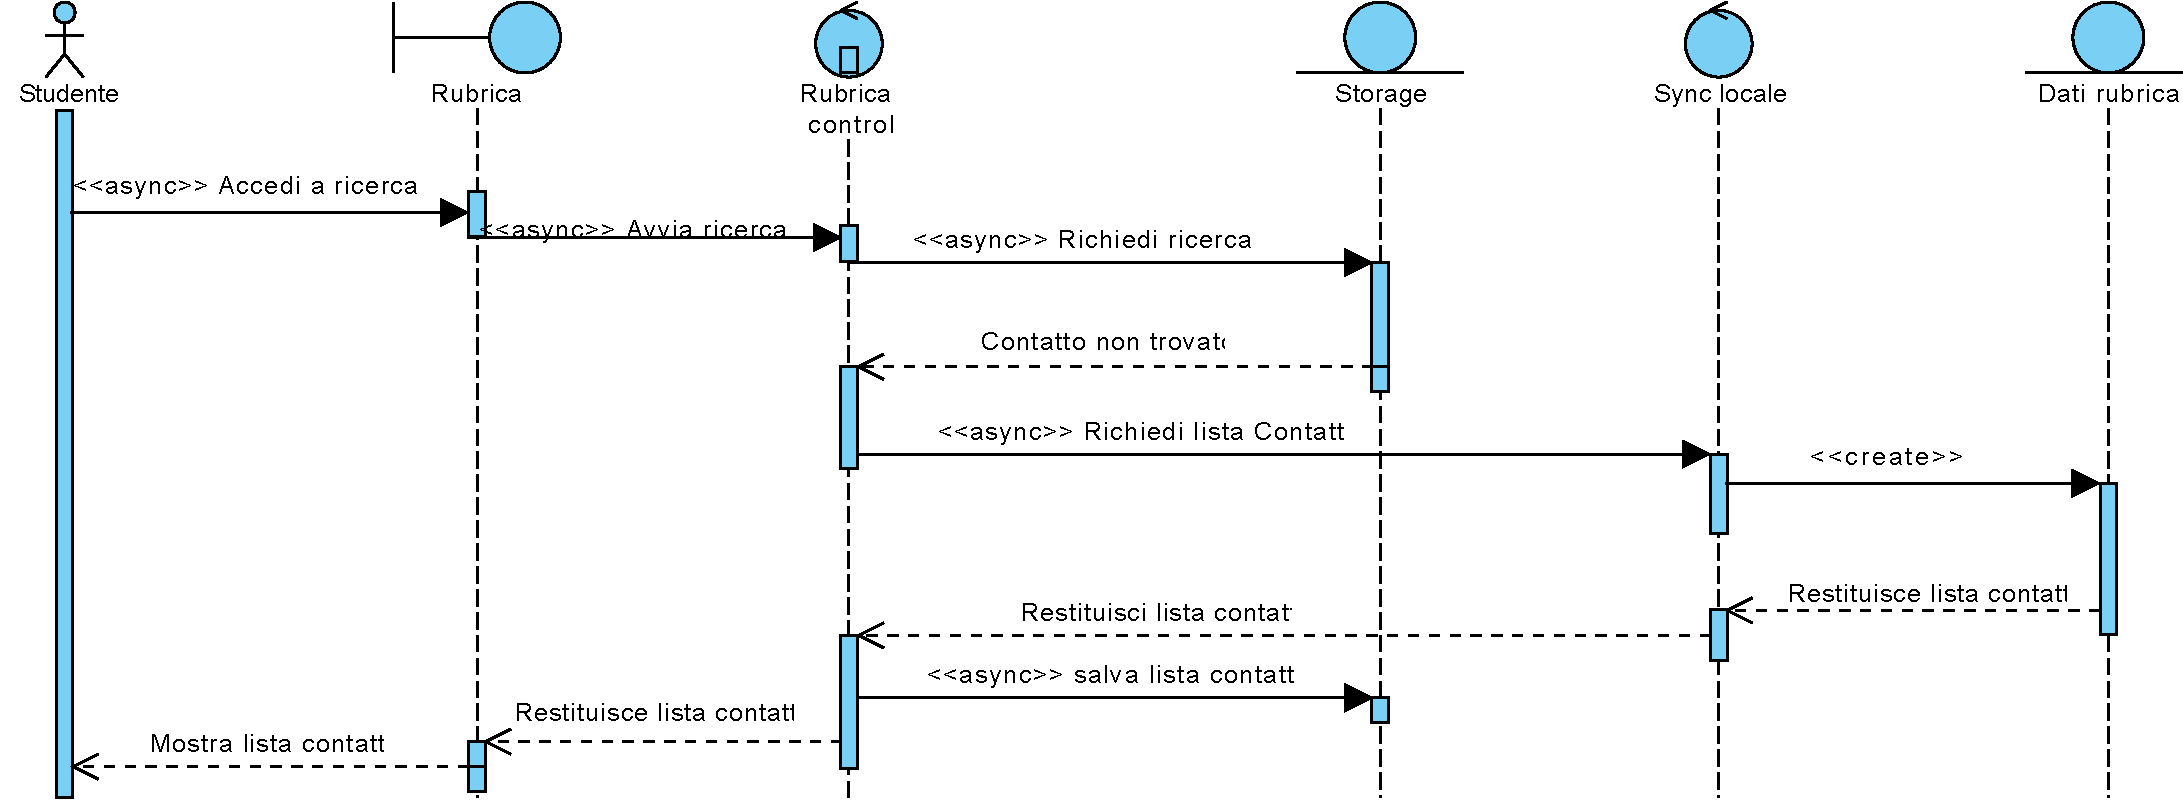
\includegraphics[width=0.9\textwidth]{imgs/gruppo5/sequence1.pdf}
	\caption{Ricerca non filtarta}
	\label{fig:seq1-rubrica}
\end{figure}

\begin{figure}[H]
\centering
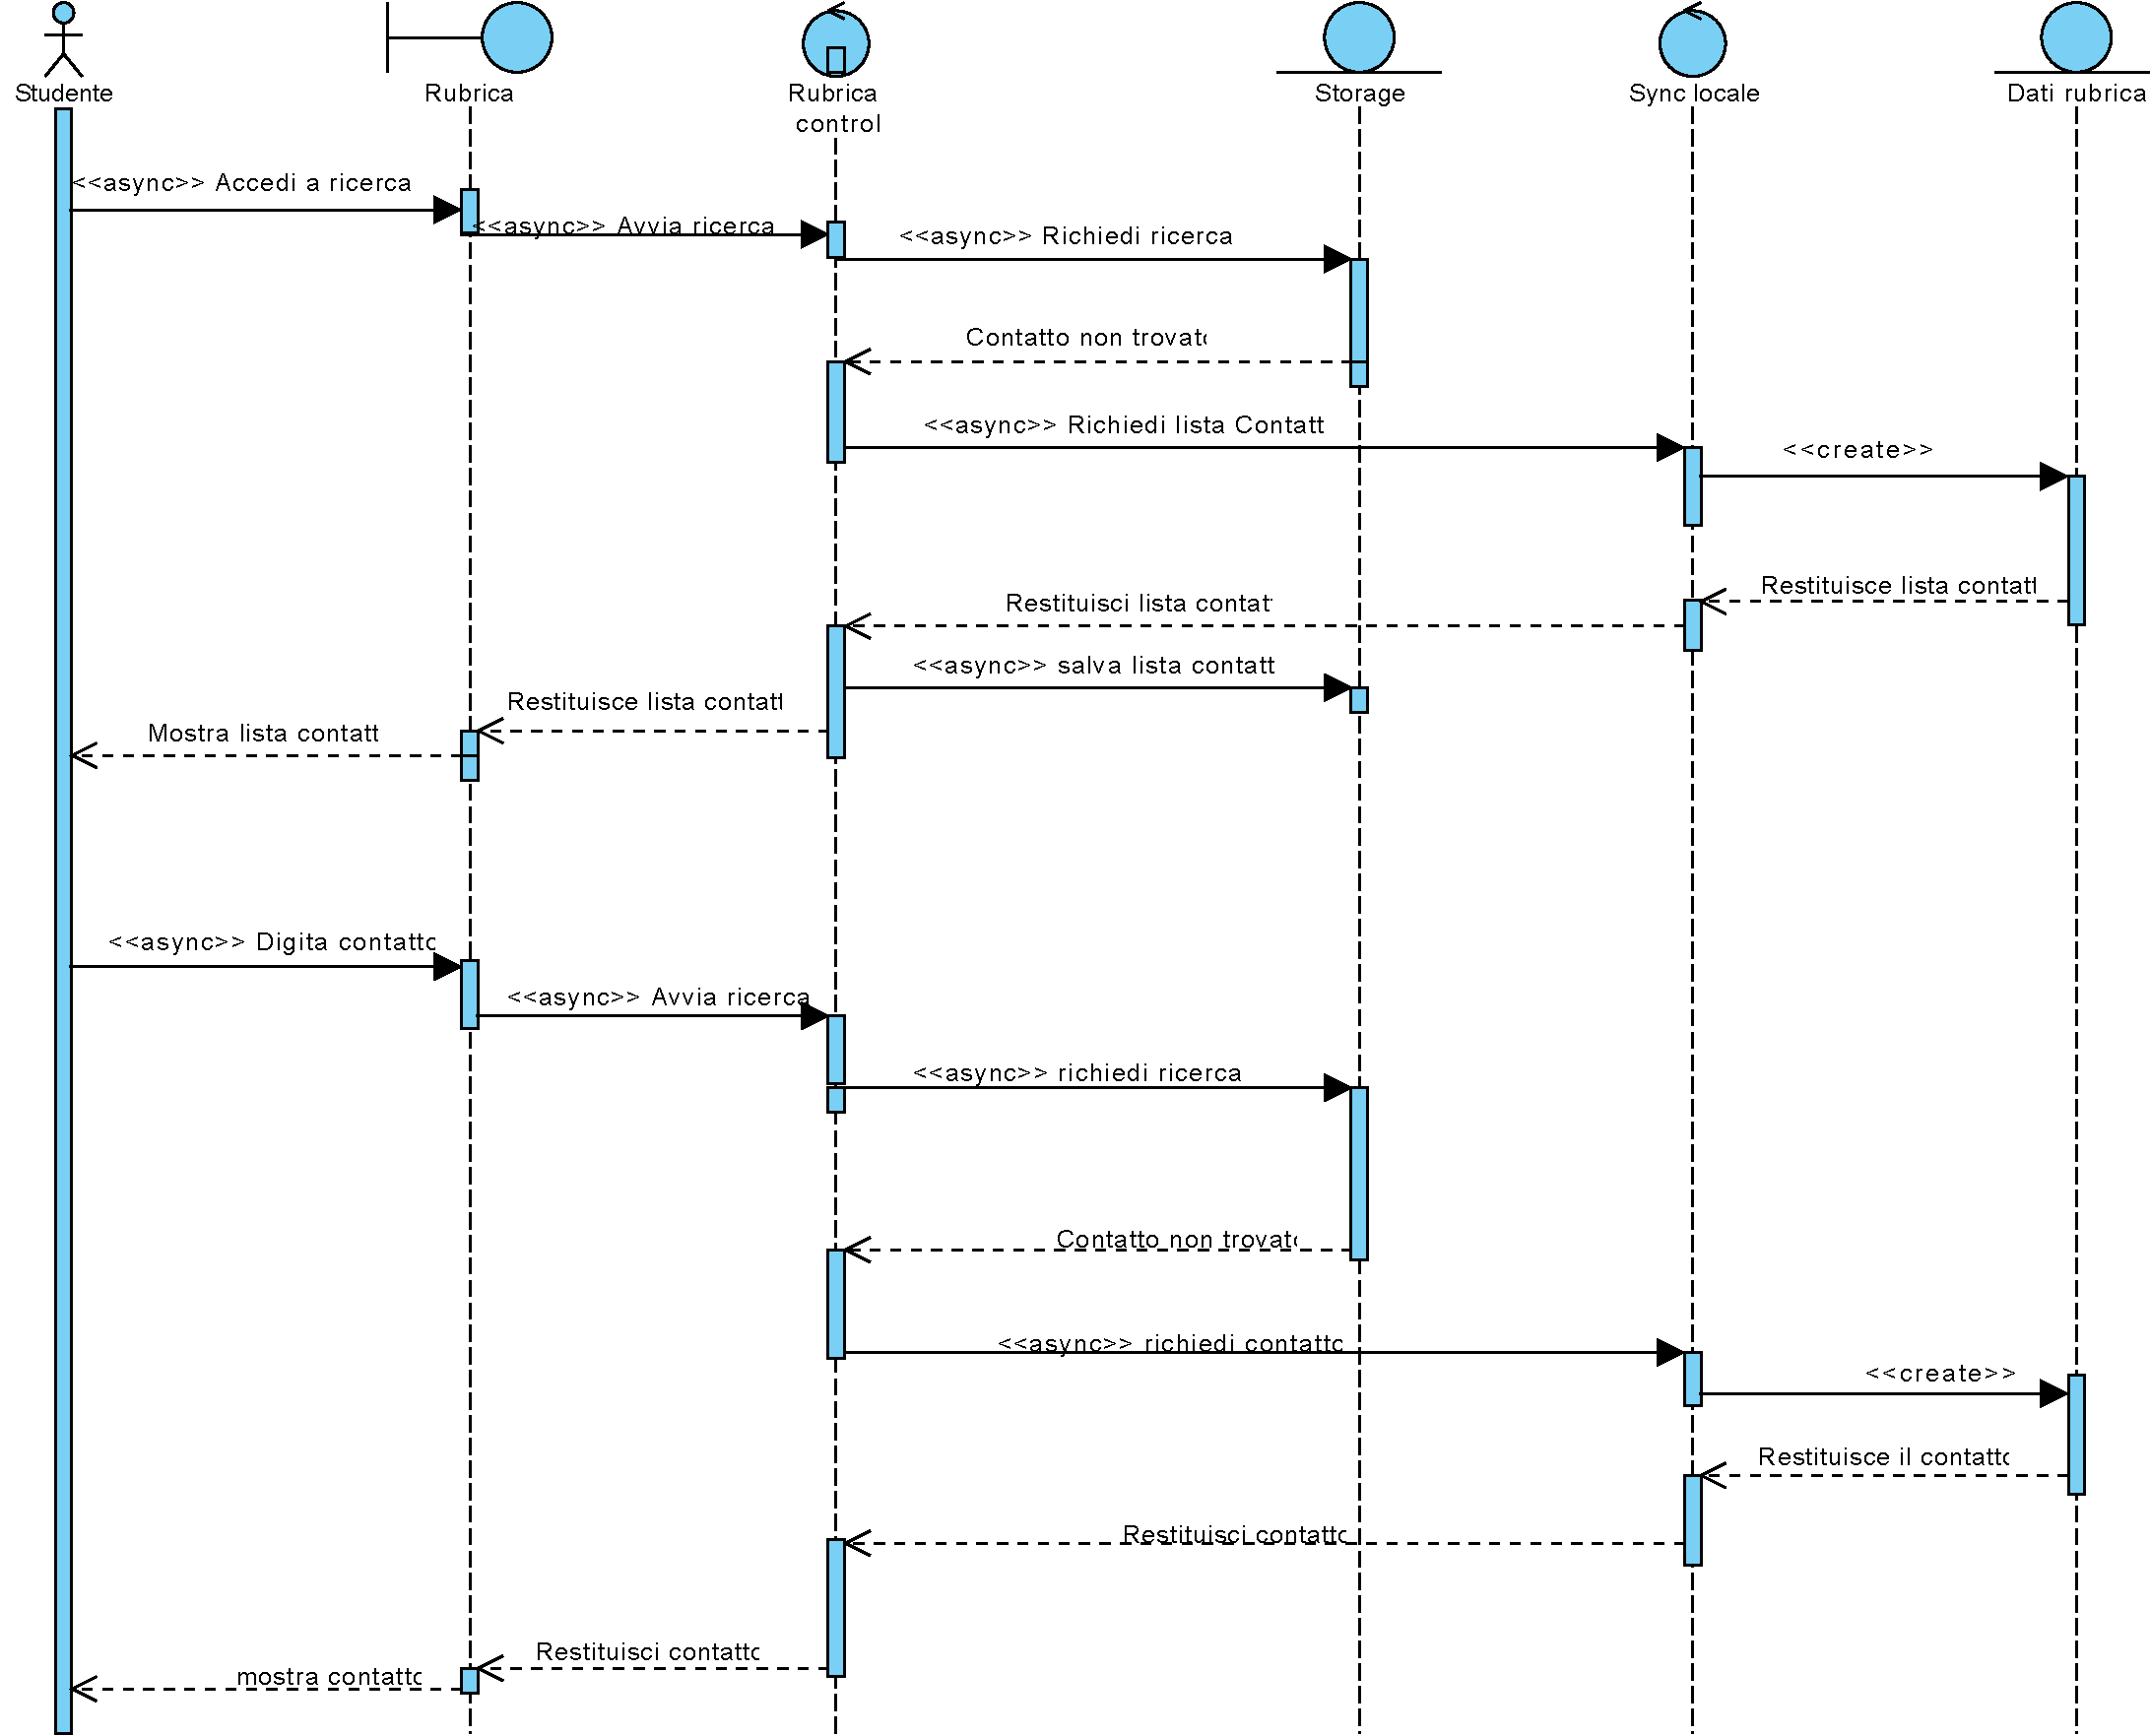
\includegraphics[width=0.9\textwidth]{imgs/gruppo5/sequence2.pdf}
\caption{Ricerca filtarta}
\label{fig:seq2-rubrica}
\end{figure}

\begin{figure}[H]
	\centering
	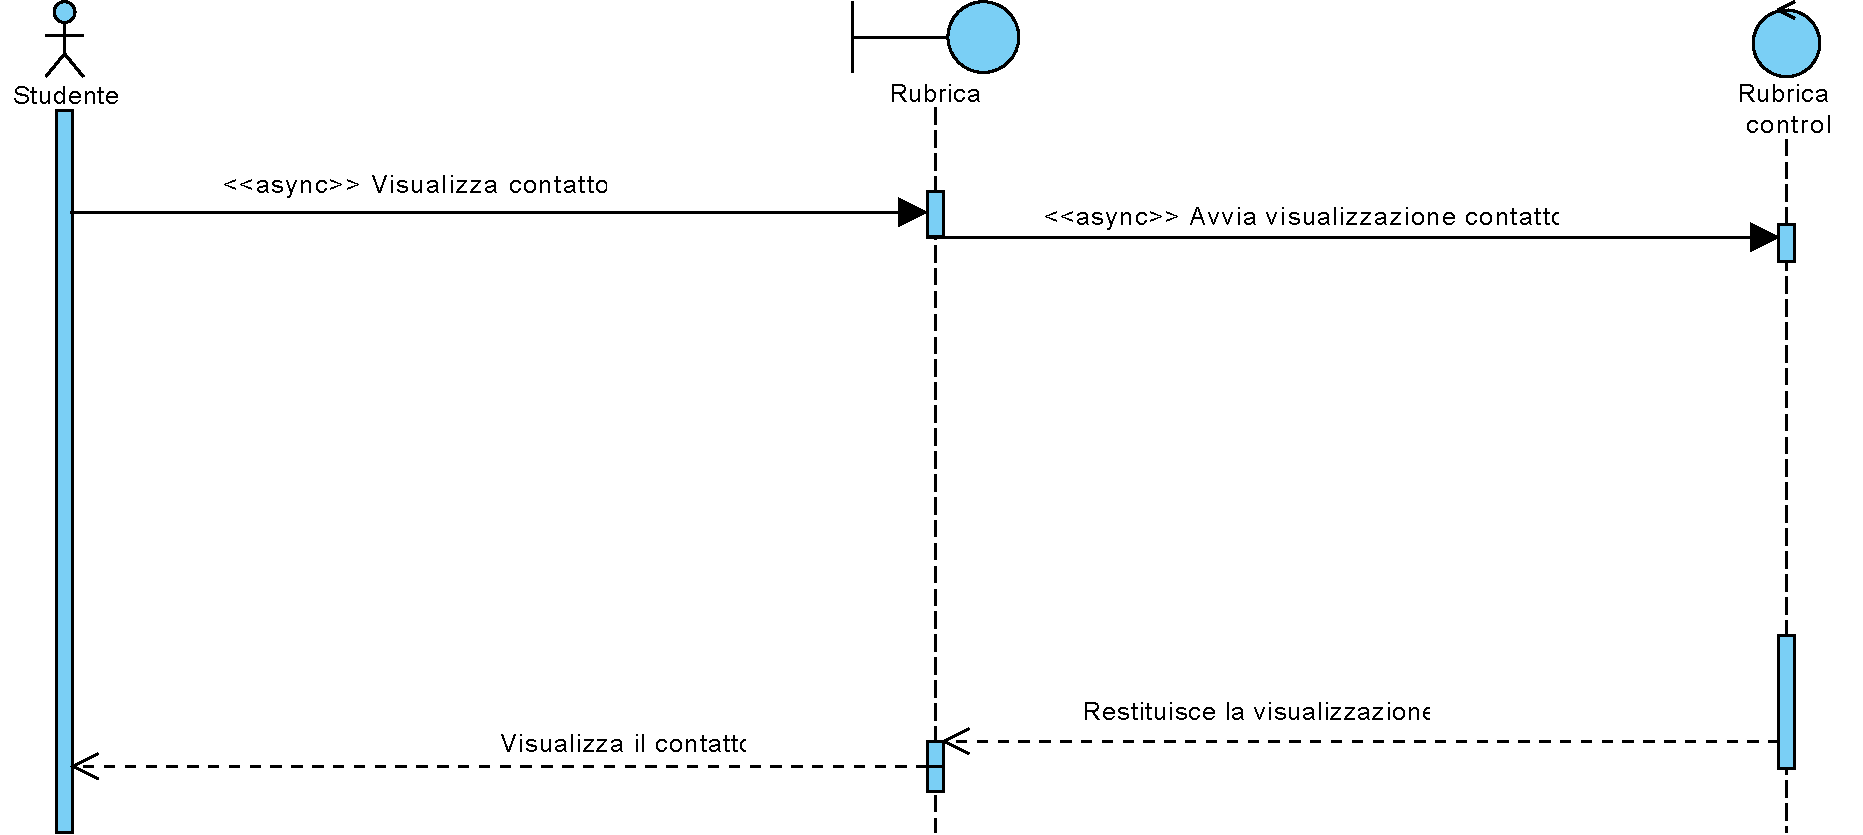
\includegraphics[width=0.9\textwidth]{imgs/gruppo5/sequence3.pdf}
	\caption{Visualizza contatto}
	\label{fig:seq3-rubrica}
\end{figure}

\clearpage
\subsection{Funzionalità previsione media}
\begin{figure}[H]
	\centering
	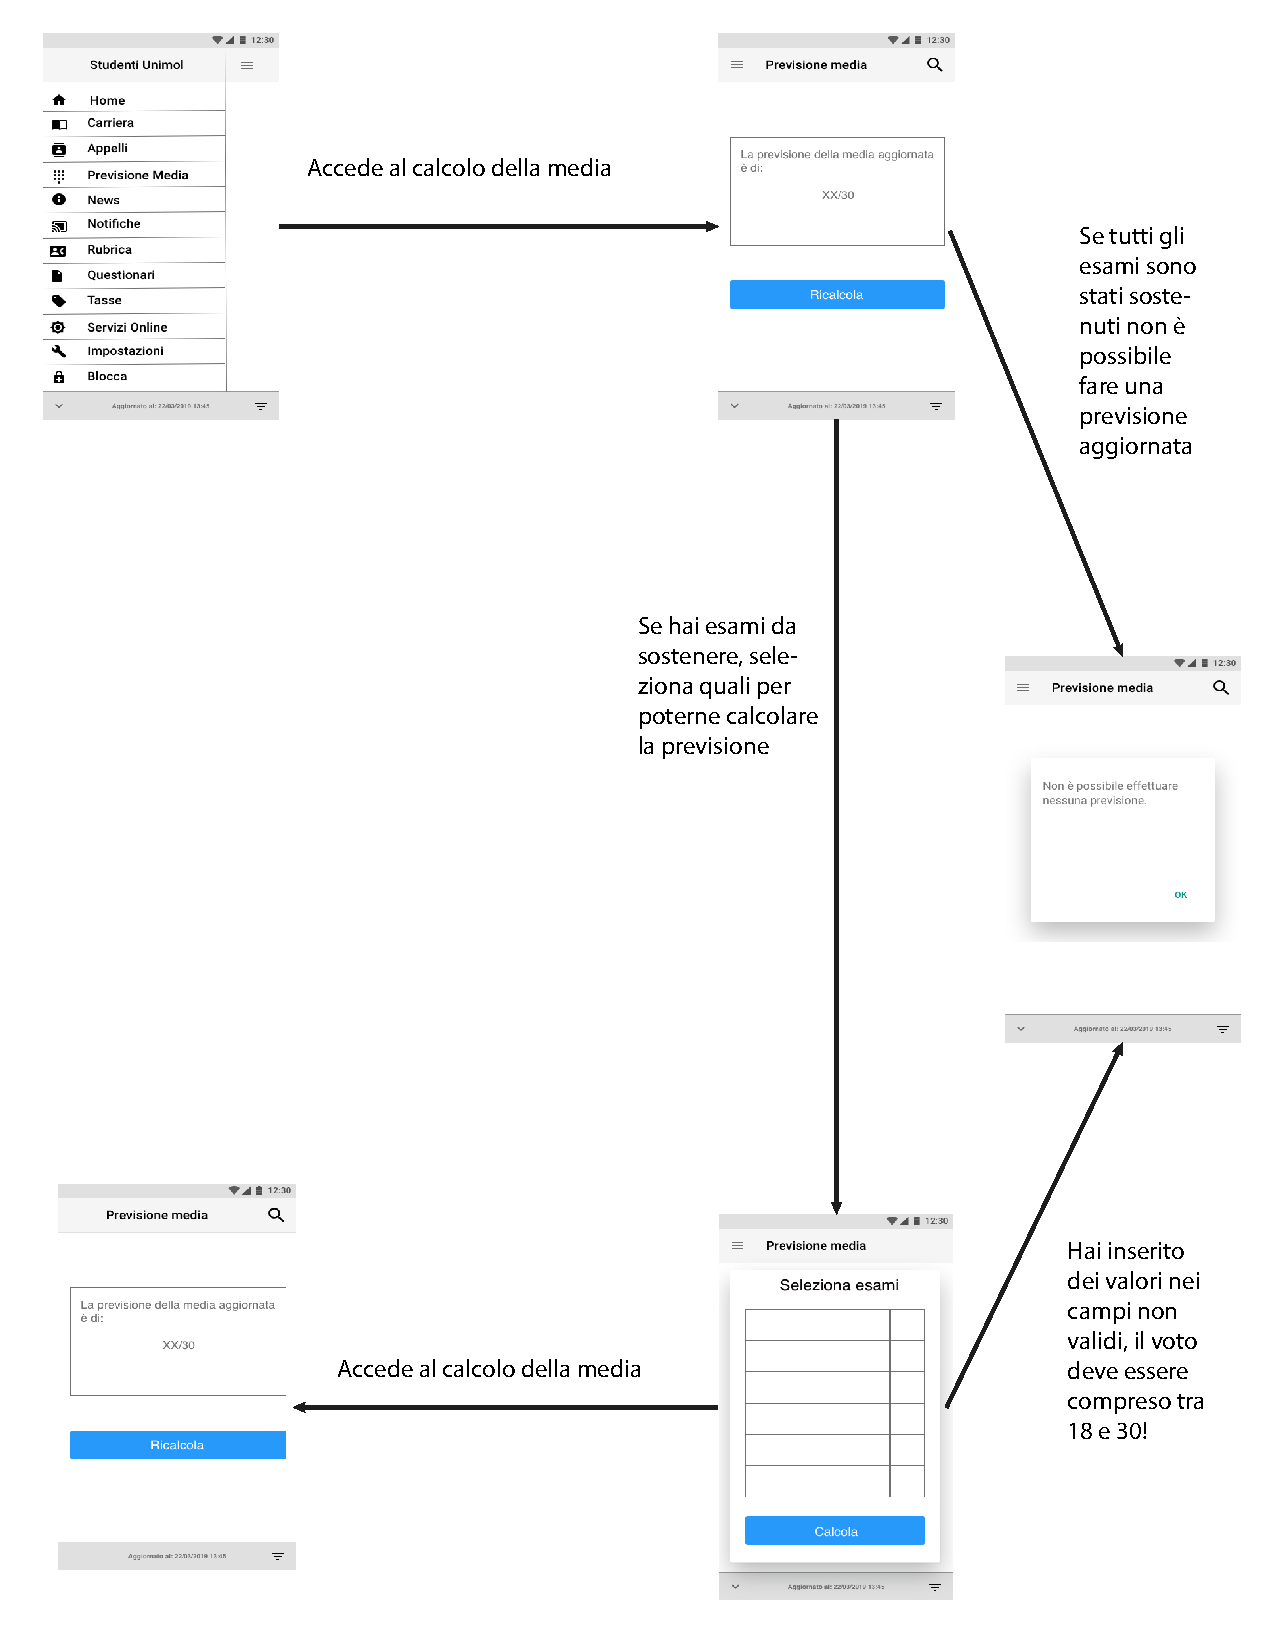
\includegraphics[width=0.9\textwidth]{imgs/gruppo3/media-activity-diagram.pdf}
	\caption{Diagramma di attività}
	\label{fig:act-rubrica}
\end{figure}

\clearpage
\section{Casi d'uso}

\subsection{Funzionalità Gestione Piano di Studio}
\label{req:gestionePianoStudio}
\paragraph{Visualizza corsi \\}
Questo caso d’uso consentirà allo studente di visualizzare i corsi afferenti al suo piano di studio e includerà il caso d’uso \textit{getJson} passandogli l’ID del servizio per ottenere la lista di tutti i corsi. Quest’ultimo elaborerà la richiesta e restituirà i dati relativi ai corsi del piano di studio, dopodiché il sistema li mostrerà allo studente. Segue il diagramma dei casi d'uso corrispondente a questo caso d'uso: \ref{diag:gestionePianoStudio}; è possibile prendere visione anche del diagramma di sequenza (\ref{diag:visualizzaCorsiSD}) e del diagramma delle attività (\ref{diag:visualizzaCorsiAD}). \\ 

\begin{tabular}{| p{\useCaseLeft} | p{\useCaseNum} | p{\useCaseTwoCol} | p{\useCaseTwoCol} |}
	\hline
	\textbf{Nome caso d'uso} & \multicolumn{3}{p{\useCaseMulticol} |}{\textbf{Visualizza corsi}} \\
	\hline
	\textbf{Attori partecipanti} & \multicolumn{3}{p{\useCaseMulticol} |}{Iniziato da \textit{Studente}.} \\
	\hline
	\textbf{Condizioni d'ingresso} & \multicolumn{3}{p{\useCaseMulticol} |}{Lo studente si trova nella sezione \textit{Piano di studio.}} \\
	\hline
	\textbf{Flusso degli eventi} & \textbf{\#} & \textbf{Studente} & \textbf{Sistema} \\
	\hline
	\textbf{} & \textbf{1} & Visualizza l’ultima copia dei corsi salvata nello \textit{storage.} & \textbf{} \\
	\hline
	\textbf{} & \textbf{2} & \textbf{} & Include il caso d’uso \textit{getJson} passandogli l’ID del servizio per la visualizzazione dei corsi. \\
	\hline
	\textbf{} & \textbf{3} & \textbf{} & Ottiene i corsi del piano di studio aggiornati e li mostra a video. \\
	\hline
	\textbf{Eccezioni} & \multicolumn{3}{p{\useCaseMulticol} |}{} \\
	\hline
	\textbf{Condizioni d'uscita} & \multicolumn{3}{p{\useCaseMulticol} |}{Lo studente visualizza i corsi aggiornati del piano di studio.} \\
	\hline
\end{tabular}
\newpage

\paragraph{Ricerca corsi \\}
Questo caso d’uso consentirà allo studente di ricercare i corsi utilizzando delle parole chiave. Il sistema, dopo aver eseguito la ricerca, mostrerà i corsi trovati. Segue il diagramma dei casi d'uso corrispondente a questo caso d'uso: \ref{diag:gestionePianoStudio}. È possibile prendere visione anche del diagramma di sequenza (\ref{diag:ricercaCorsiSD}) e del diagramma delle attività (\ref{diag:ricercaCorsiAD}). \\ \\

\begin{tabular}{| p{\useCaseLeft} | p{\useCaseNum} | p{\useCaseTwoCol} | p{\useCaseTwoCol} |}
	\hline
	\textbf{Nome caso d'uso} & \multicolumn{3}{p{\useCaseMulticol} |}{\textbf{Ricerca corsi}} \\
	\hline
	\textbf{Attori partecipanti} & \multicolumn{3}{p{\useCaseMulticol} |}{Iniziato da \textit{Studente}.} \\
	\hline
	\textbf{Condizioni d'ingresso} & \multicolumn{3}{p{\useCaseMulticol} |}{Lo studente visualizza i corsi del piano di studio.} \\
	\hline
	\textbf{Flusso degli eventi} & \textbf{\#} & \textbf{Studente} & \textbf{Sistema} \\
	\hline
	\textbf{} & \textbf{1} & Inserisce delle parole chiave. & \textbf{} \\
	\hline
	\textbf{} & \textbf{2} & \textbf{} & Esegue la ricerca. \\
	\hline
	\textbf{} & \textbf{3} & \textbf{} & Mostra i corsi che corrispondono alle parole chiave. \\
	\hline
	\textbf{Eccezioni} & \multicolumn{3}{p{\useCaseMulticol} |}{\textbf{2.1} Nessun risultato} \\
	\hline
	\textbf{Condizioni d'uscita} & \multicolumn{3}{p{\useCaseMulticol} |}{Lo studente visualizza i corsi trovati.} \\
	\hline
\end{tabular}
\newpage

\paragraph{Filtra corsi con memorizzazione \\}
Questo caso d’uso consentirà allo studente di filtrare i corsi in base ad uno o più filtri. Il sistema, dopo aver filtrato l’elenco, mostrerà la lista di corsi filtrati. Lo studente avrà la possibilità di memorizzare i filtri nello \textit{storage} per visualizzare i dati filtrati ad ogni nuovo accesso alla sezione. Segue il diagramma dei casi d'uso corrispondente a questo caso d'uso: 
\ref{diag:gestionePianoStudio}. È possibile prendere visione anche del diagramma di sequenza (\ref{diag:filtraCorsiConMemSD}) e del diagramma delle attività (\ref{diag:filtraCorsiConMemAD}).\\ \\
\begin{tabular}{| p{\useCaseLeft} | p{\useCaseNum} | p{\useCaseTwoCol} | p{\useCaseTwoCol} |}
	\hline
	\textbf{Nome caso d'uso} & \multicolumn{3}{p{\useCaseMulticol} |}{\textbf{Filtra corsi con memorizzazione}} \\
	\hline
	\textbf{Attori partecipanti} & \multicolumn{3}{p{\useCaseMulticol} |}{Iniziato da \textit{Studente}.} \\
	\hline
	\textbf{Condizioni d'ingresso} & \multicolumn{3}{p{\useCaseMulticol} |}{Lo studente visualizza i corsi del piano di studio.} \\
	\hline
	\textbf{Flusso degli eventi} & \textbf{\#} & \textbf{Studente} & \textbf{Sistema} \\
	\hline
	\textbf{} & \textbf{1} & Inserisce uno o più filtri. & \textbf{} \\
	\hline
	\textbf{} & \textbf{2} & \textbf{} & Filtra l’elenco dei corsi. \\
	\hline
	\textbf{} & \textbf{3} & \textbf{} & Mostra i corsi filtrati. \\
	\hline
	\textbf{} & \textbf{4} & Sceglie di salvare i filtri. & \textbf{} \\
	\hline
	\textbf{} & \textbf{5} &  \textbf{} & Memorizza i filtri nello \textit{storage}.\\
	\hline
	\textbf{Eccezioni} & \multicolumn{3}{p{\useCaseMulticol} |}{\textbf{4.1} Nessuna memorizzazione.\newline \textbf{5.1} Nessun risultato.} \\
	\hline
	\textbf{Condizioni d'uscita} & \multicolumn{3}{p{\useCaseMulticol} |}{Lo studente visualizza i corsi filtrati ed eventualmente salva i filtri. } \\
	\hline
\end{tabular}
\newpage

\paragraph{Ordina corsi con memorizzazione \\}
Questo caso d’uso consentirà allo studente di ordinare i corsi in base ad un criterio di ordinamento. Il sistema, dopo aver ordinato l’elenco, mostrerà la lista di corsi ordinati. Lo studente avrà la possibilità di memorizzare il criterio di ordinamento nello \textit{storage}. Segue il diagramma dei casi d'uso corrispondente a questo caso d'uso: \ref{diag:gestionePianoStudio}. È possibile prendere visione anche del diagramma di sequenza (\ref{diag:ordinaCorsiConMemSD}) e del diagramma delle attività (\ref{diag:ordinaCorsiConMemAD}). \\ \\
\begin{tabular}{| p{\useCaseLeft} | p{\useCaseNum} | p{\useCaseTwoCol} | p{\useCaseTwoCol} |}
	\hline
	\textbf{Nome caso d'uso} & \multicolumn{3}{p{\useCaseMulticol} |}{\textbf{Ordina corsi con memorizzazione}} \\
	\hline
	\textbf{Attori partecipanti} & \multicolumn{3}{p{\useCaseMulticol} |}{Iniziato da \textit{Studente}.} \\
	\hline
	\textbf{Condizioni d'ingresso} & \multicolumn{3}{p{\useCaseMulticol} |}{Lo studente visualizza i corsi del piano di studio.} \\
	\hline
	\textbf{Flusso degli eventi} & \textbf{\#} & \textbf{Studente} & \textbf{Sistema} \\
	\hline
	\textbf{} & \textbf{1} & Inserisce un criterio di ordinamento. & \textbf{} \\
	\hline
	\textbf{} & \textbf{2} & \textbf{} & Ordina l’elenco dei corsi. \\
	\hline
	\textbf{} & \textbf{3} & \textbf{} & Mostra i corsi ordinati. \\
	\hline
	\textbf{} & \textbf{4} & Sceglie di salvare il criterio di ordinamento selezionato. & \textbf{} \\
	\hline
	\textbf{} & \textbf{5} &  \textbf{} & Memorizza nello \textit{storage} il criterio di ordinamento.\\
	\hline
	\textbf{Eccezioni} & \multicolumn{3}{p{\useCaseMulticol} |}{\textbf{3.1} Nessuna memorizzazione.} \\
	\hline
	\textbf{Condizioni d'uscita} & \multicolumn{3}{p{\useCaseMulticol} |}{Lo studente visualizza i corsi ordinati ed eventualmente salva il criterio di ordinamento.} \\
	\hline
\end{tabular}

\clearpage

\subsection{Funzionalità Visualizza dettagli corso}
\label{req:visualizzaDettagliCorso}
\paragraph{Visualizza dettagli corso \\}
Questo caso d’uso consentirà allo studente di visualizzare i dettagli di un corso e includerà il caso d’uso \textit{getJson} passandogli l’ID del servizio per ottenere i dettagli del corso selezionato. Quest’ultimo elaborerà la richiesta e restituirà i dati relativi al corso selezionato. Il sistema mostrerà allo studente i dettagli del corso selezionato. Segue il diagramma dei casi d'uso corrispondente a questo caso d'uso: \ref{diag:gestionePianoStudio}. È possibile prendere visione anche del diagramma di sequenza (\ref{diag:visualizzaDettagliCorsoSD}) e del diagramma delle attività (\ref{diag:visualizzaDettagliCorsoAD}). \\ \\
\begin{tabular}{| p{\useCaseLeft} | p{\useCaseNum} | p{\useCaseTwoCol} | p{\useCaseTwoCol} |}
	\hline
	\textbf{Nome caso d'uso} & \multicolumn{3}{p{\useCaseMulticol} |}{\textbf{Visualizza dettagli corso}} \\
	\hline
	\textbf{Attori partecipanti} & \multicolumn{3}{p{\useCaseMulticol} |}{Iniziato da \textit{Studente}.} \\
	\hline
	\textbf{Condizioni d'ingresso} & \multicolumn{3}{p{\useCaseMulticol} |}{Lo studente visualizza i corsi del piano di studio.} \\
	\hline
	\textbf{Flusso degli eventi} & \textbf{\#} & \textbf{Studente} & \textbf{Sistema} \\
	\hline
	\textbf{} & \textbf{1} & Seleziona un corso di cui visualizzare i dettagli. & \textbf{} \\
	\hline
	\textbf{} & \textbf{2} & \textbf{} & Include il caso d’uso \textit{getJson} passandogli l’ID del servizio. \\
	\hline
	\textbf{} & \textbf{3} & \textbf{} & Mostra i dettagli relativi al corso selezionato. \\
	\hline
	\textbf{Eccezioni} & \multicolumn{3}{p{\useCaseMulticol} |}{} \\
	\hline
	\textbf{Condizioni d'uscita} & \multicolumn{3}{p{\useCaseMulticol} |}{Lo studente visualizza i dettagli relativi al corso selezionato.} \\
	\hline
\end{tabular}

\clearpage

\subsection{Funzionalità Gestione appelli}
\clearpage
%\paragraph{Visualizza appelli disponibil}
\begin{figure}
	\centering
	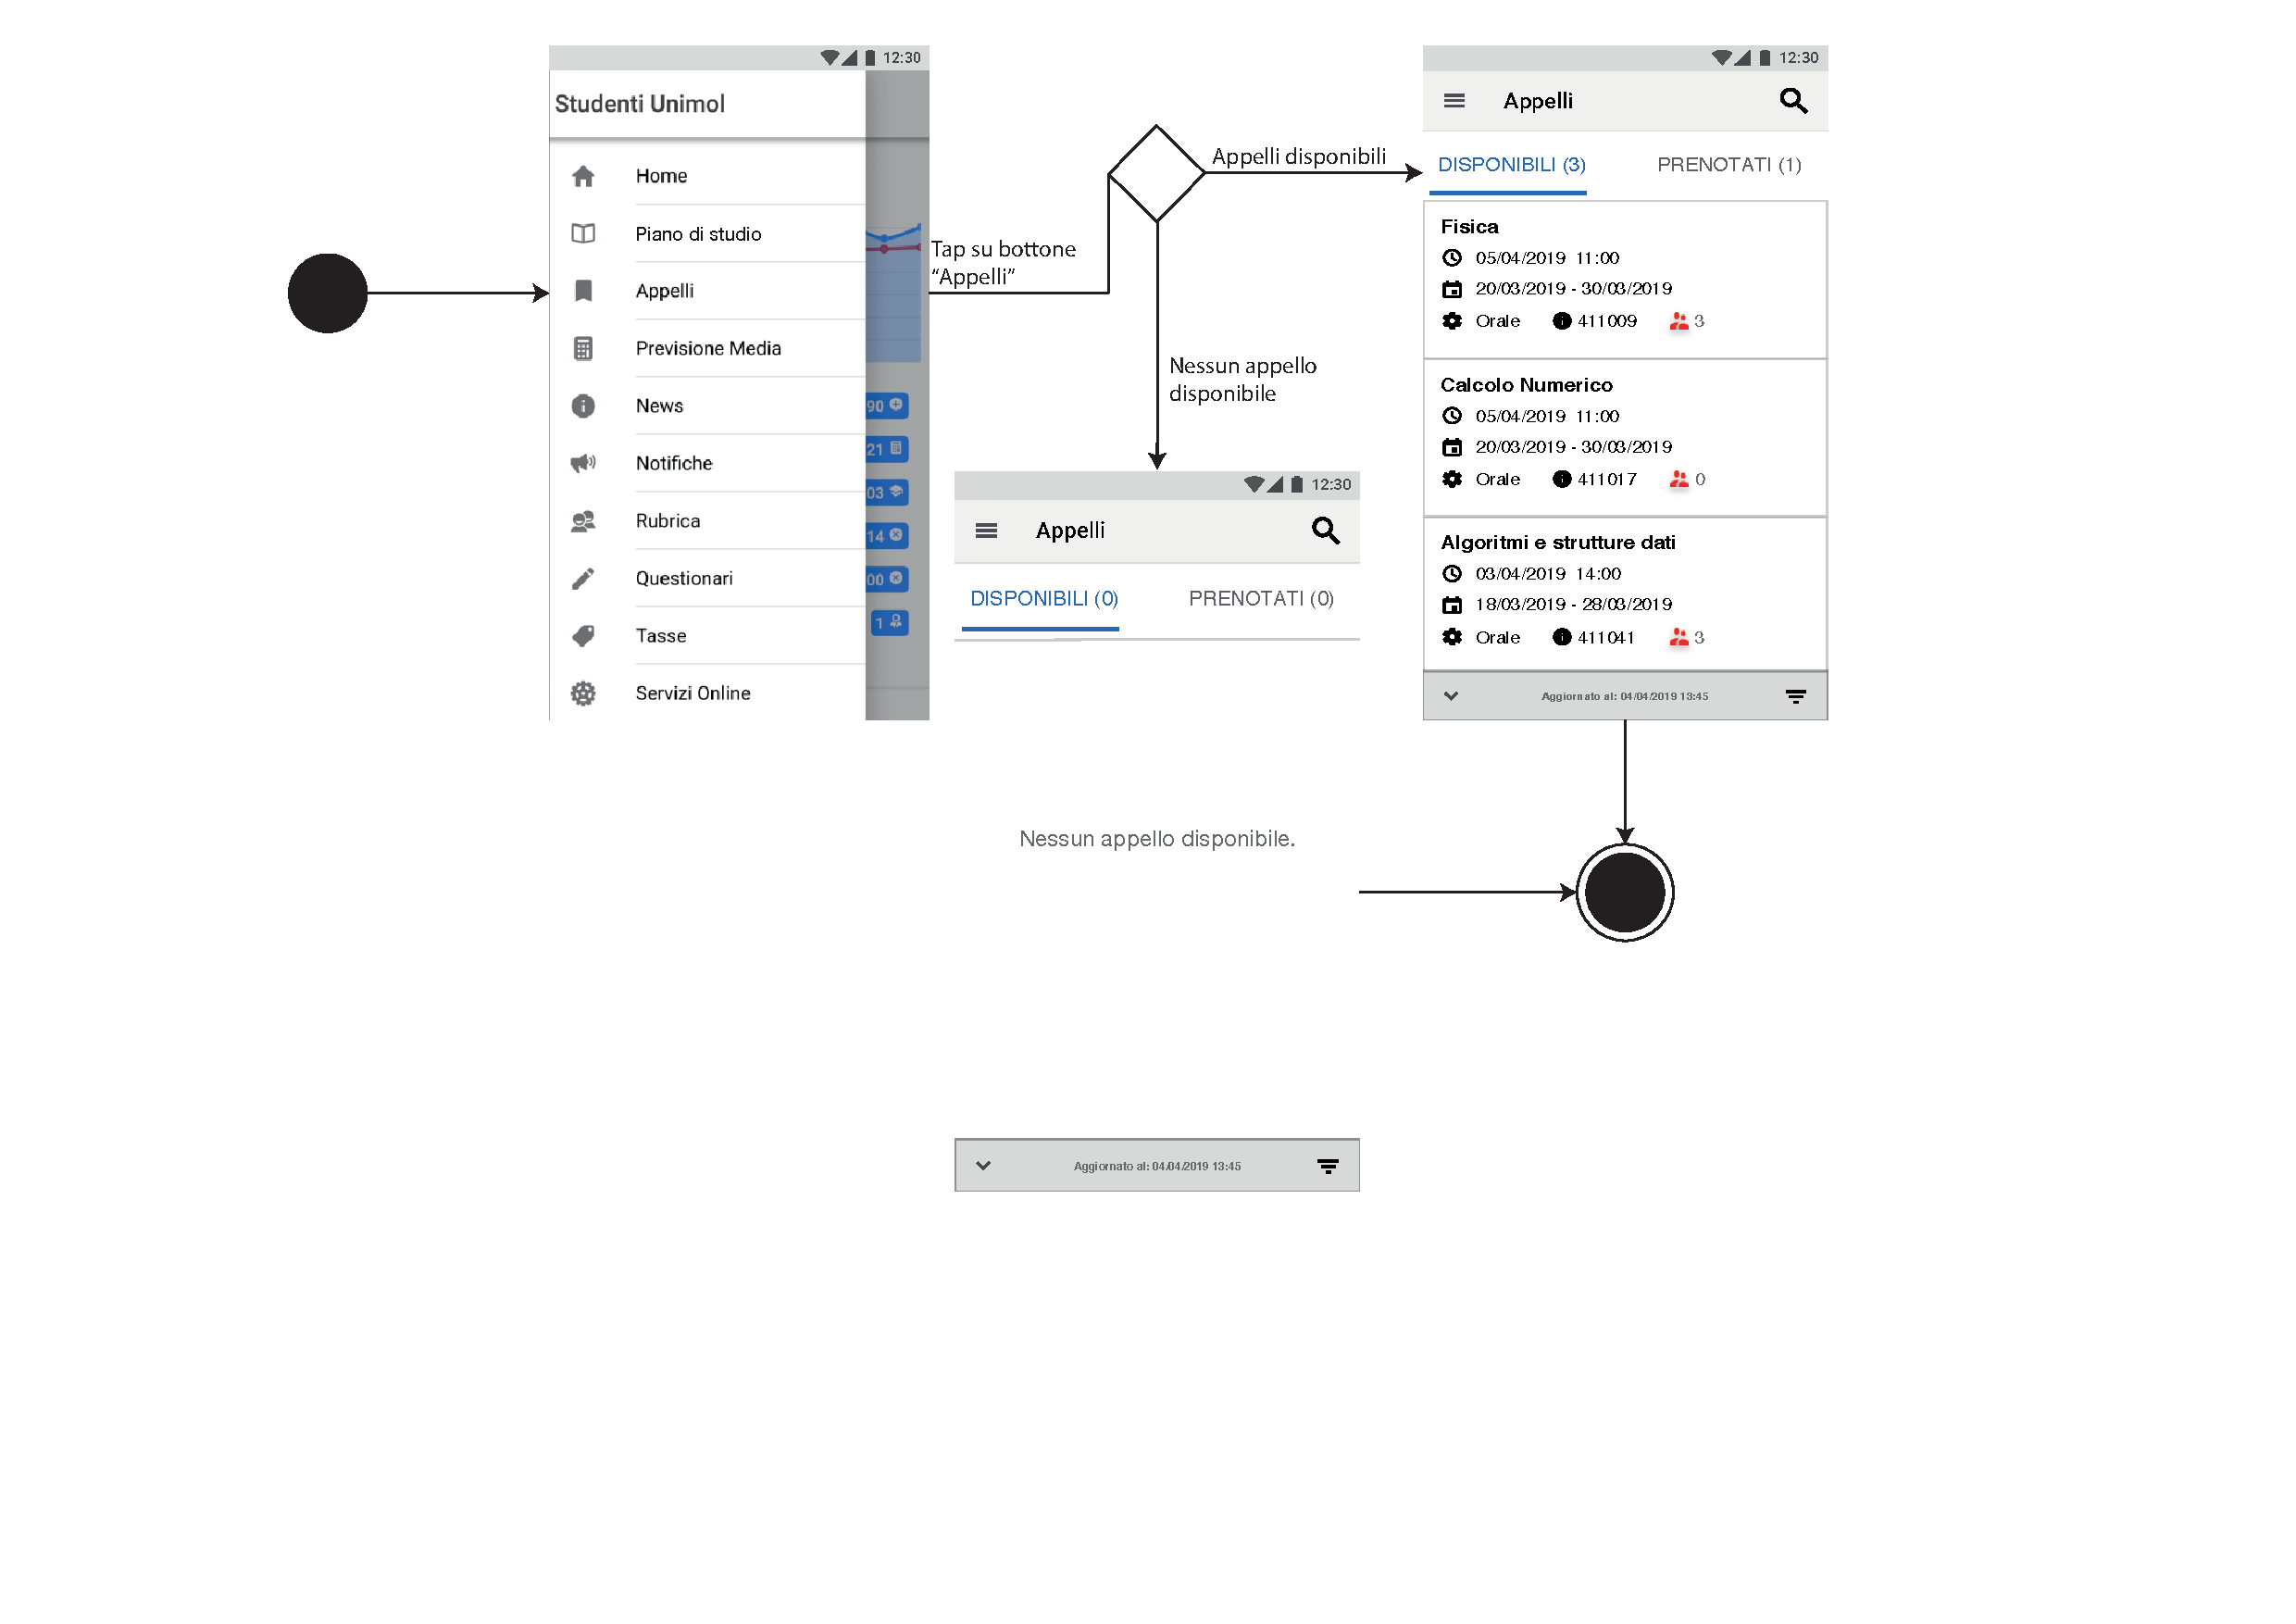
\includegraphics[width=6in]{imgs/gruppo1/activity_diagrams/AD6_visualizza_appelli_disponibili.pdf}
	\caption{Activity Diagram - Visualizza appelli disponibili}
	\label{diag:visualizzaAppelliDisponibiliAD}
\end{figure}
\newpage

%\paragraph{Visualizza appelli prenotati}
\begin{figure}
	\centering
	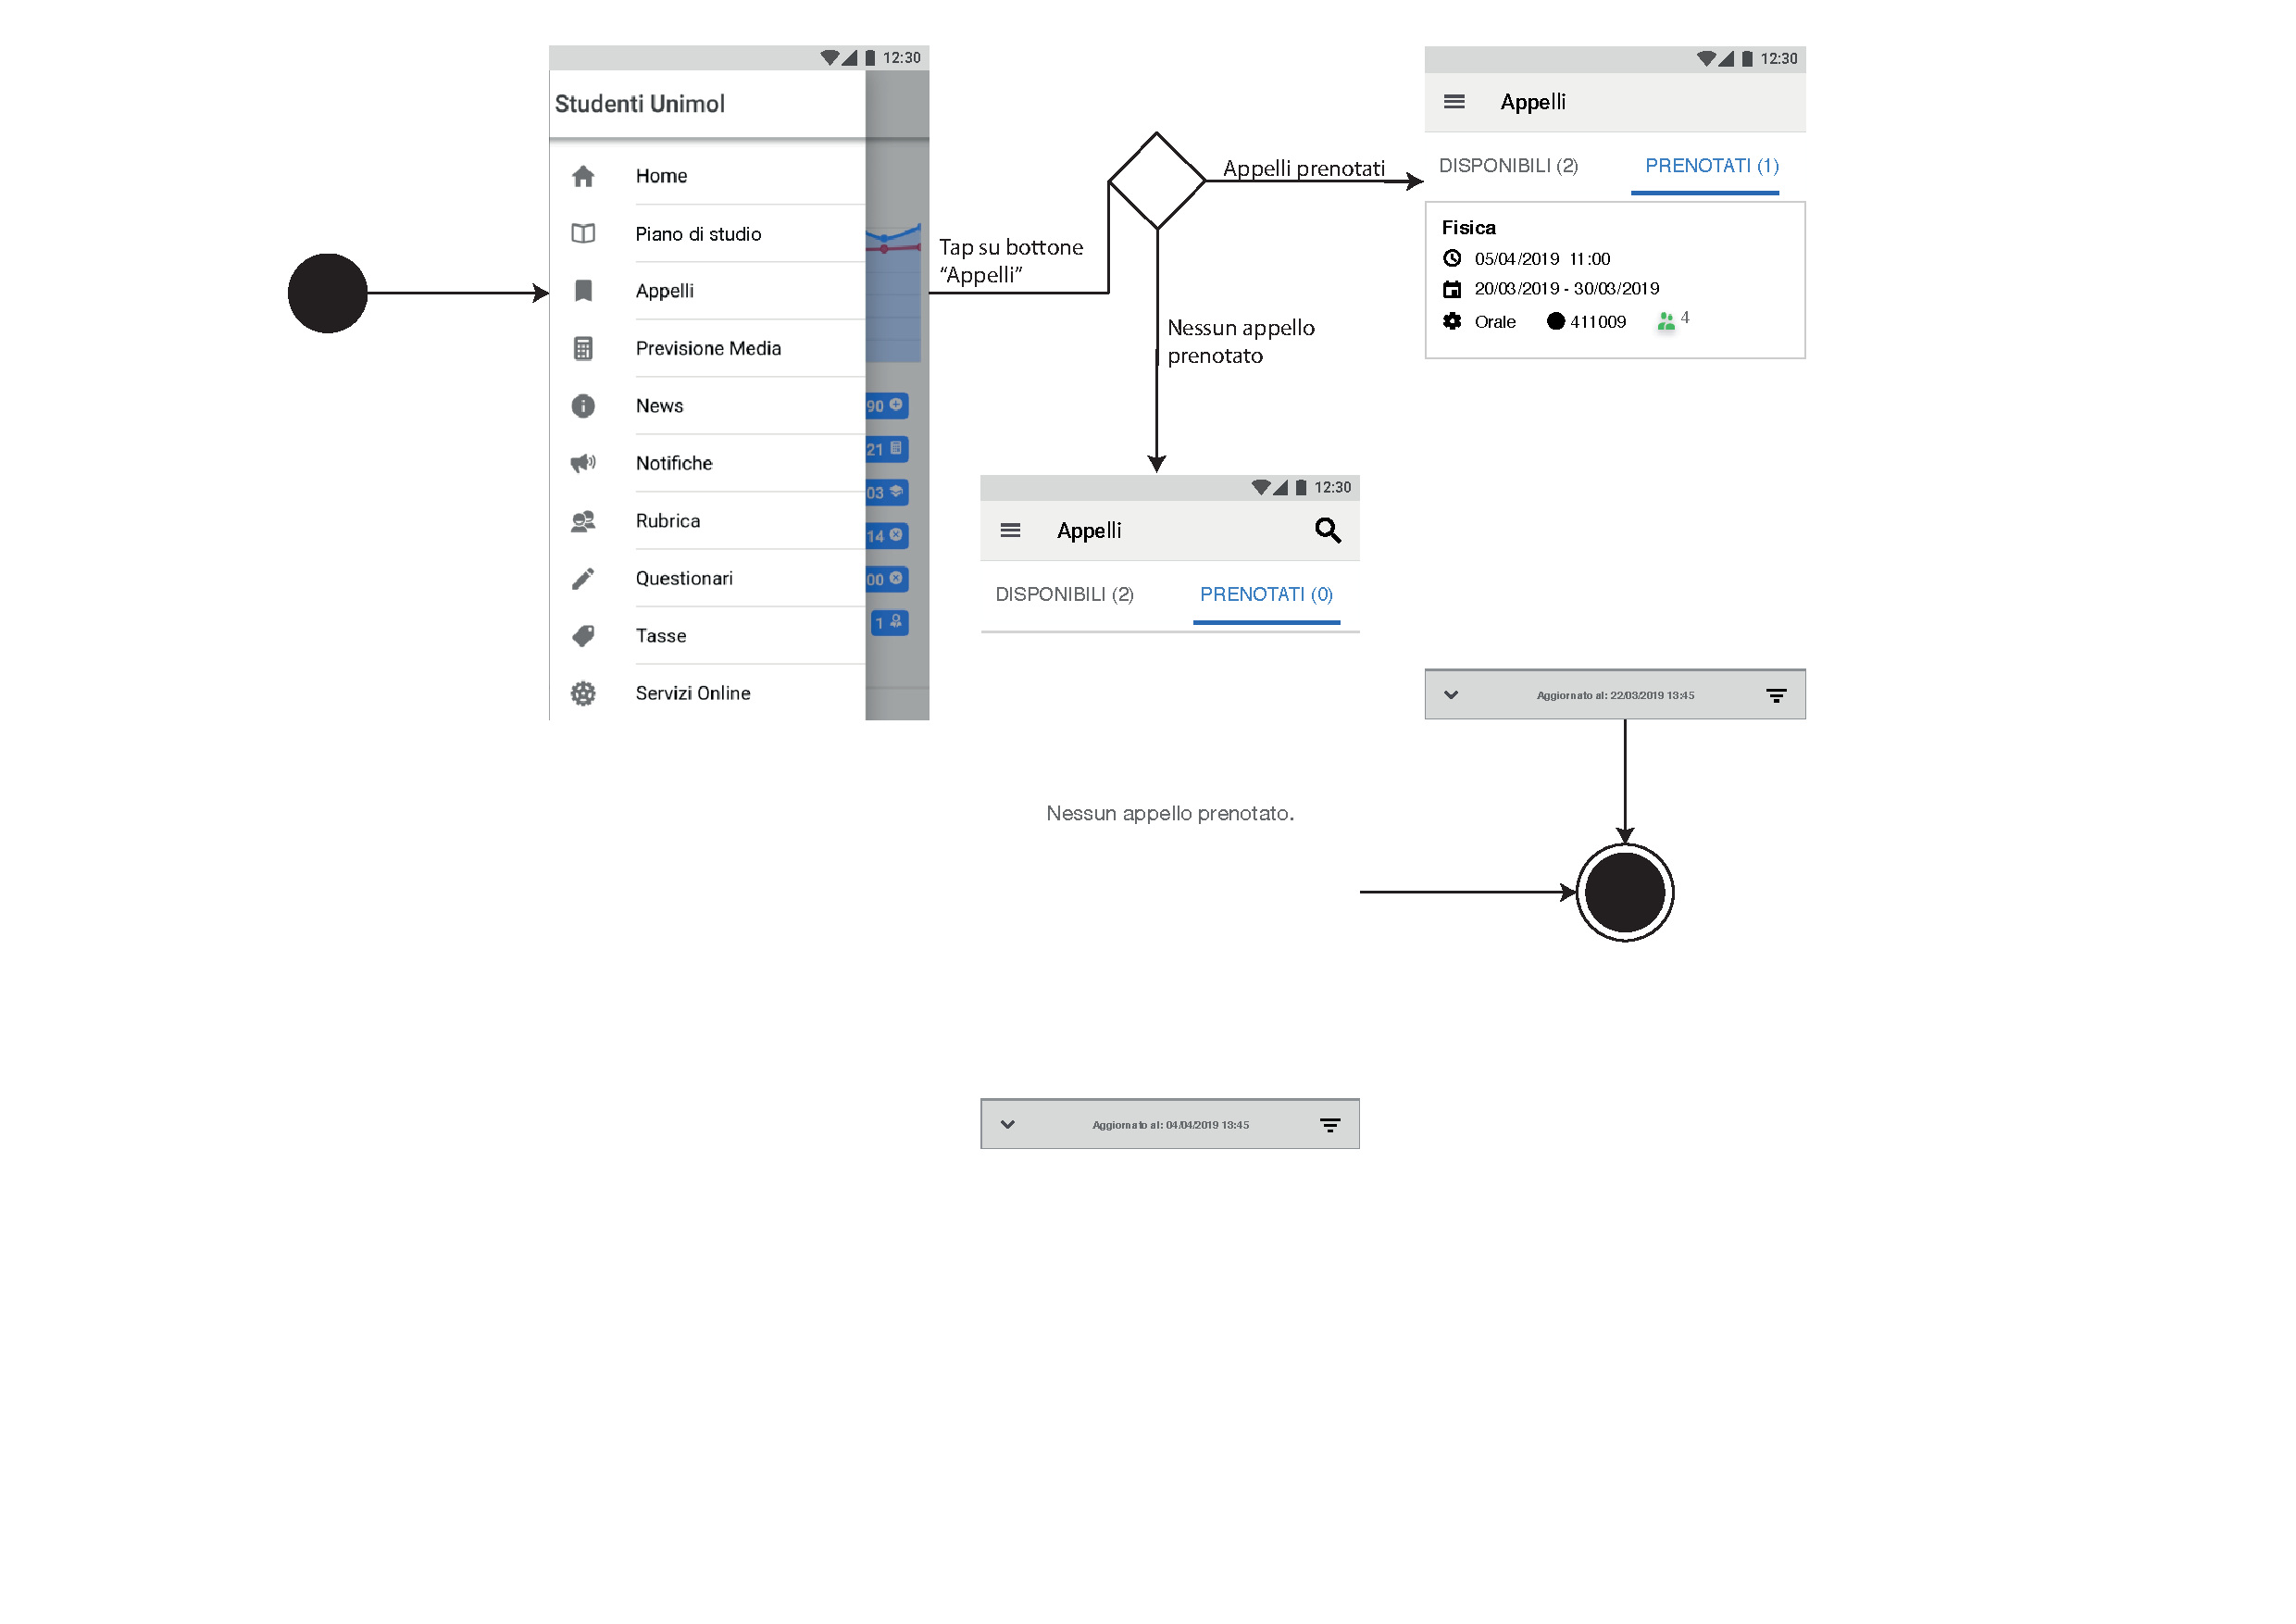
\includegraphics[width=6in]{imgs/gruppo1/activity_diagrams/AD7_visualizza_appelli_prenotati.pdf}
	\caption{Activity Diagram - Visualizza appelli prenotati}
	\label{diag:visualizzaAppelliPrenotatiAD}
\end{figure}
\newpage

%\paragraph{Ricerca appelli disponibili}
\begin{figure}
	\centering
	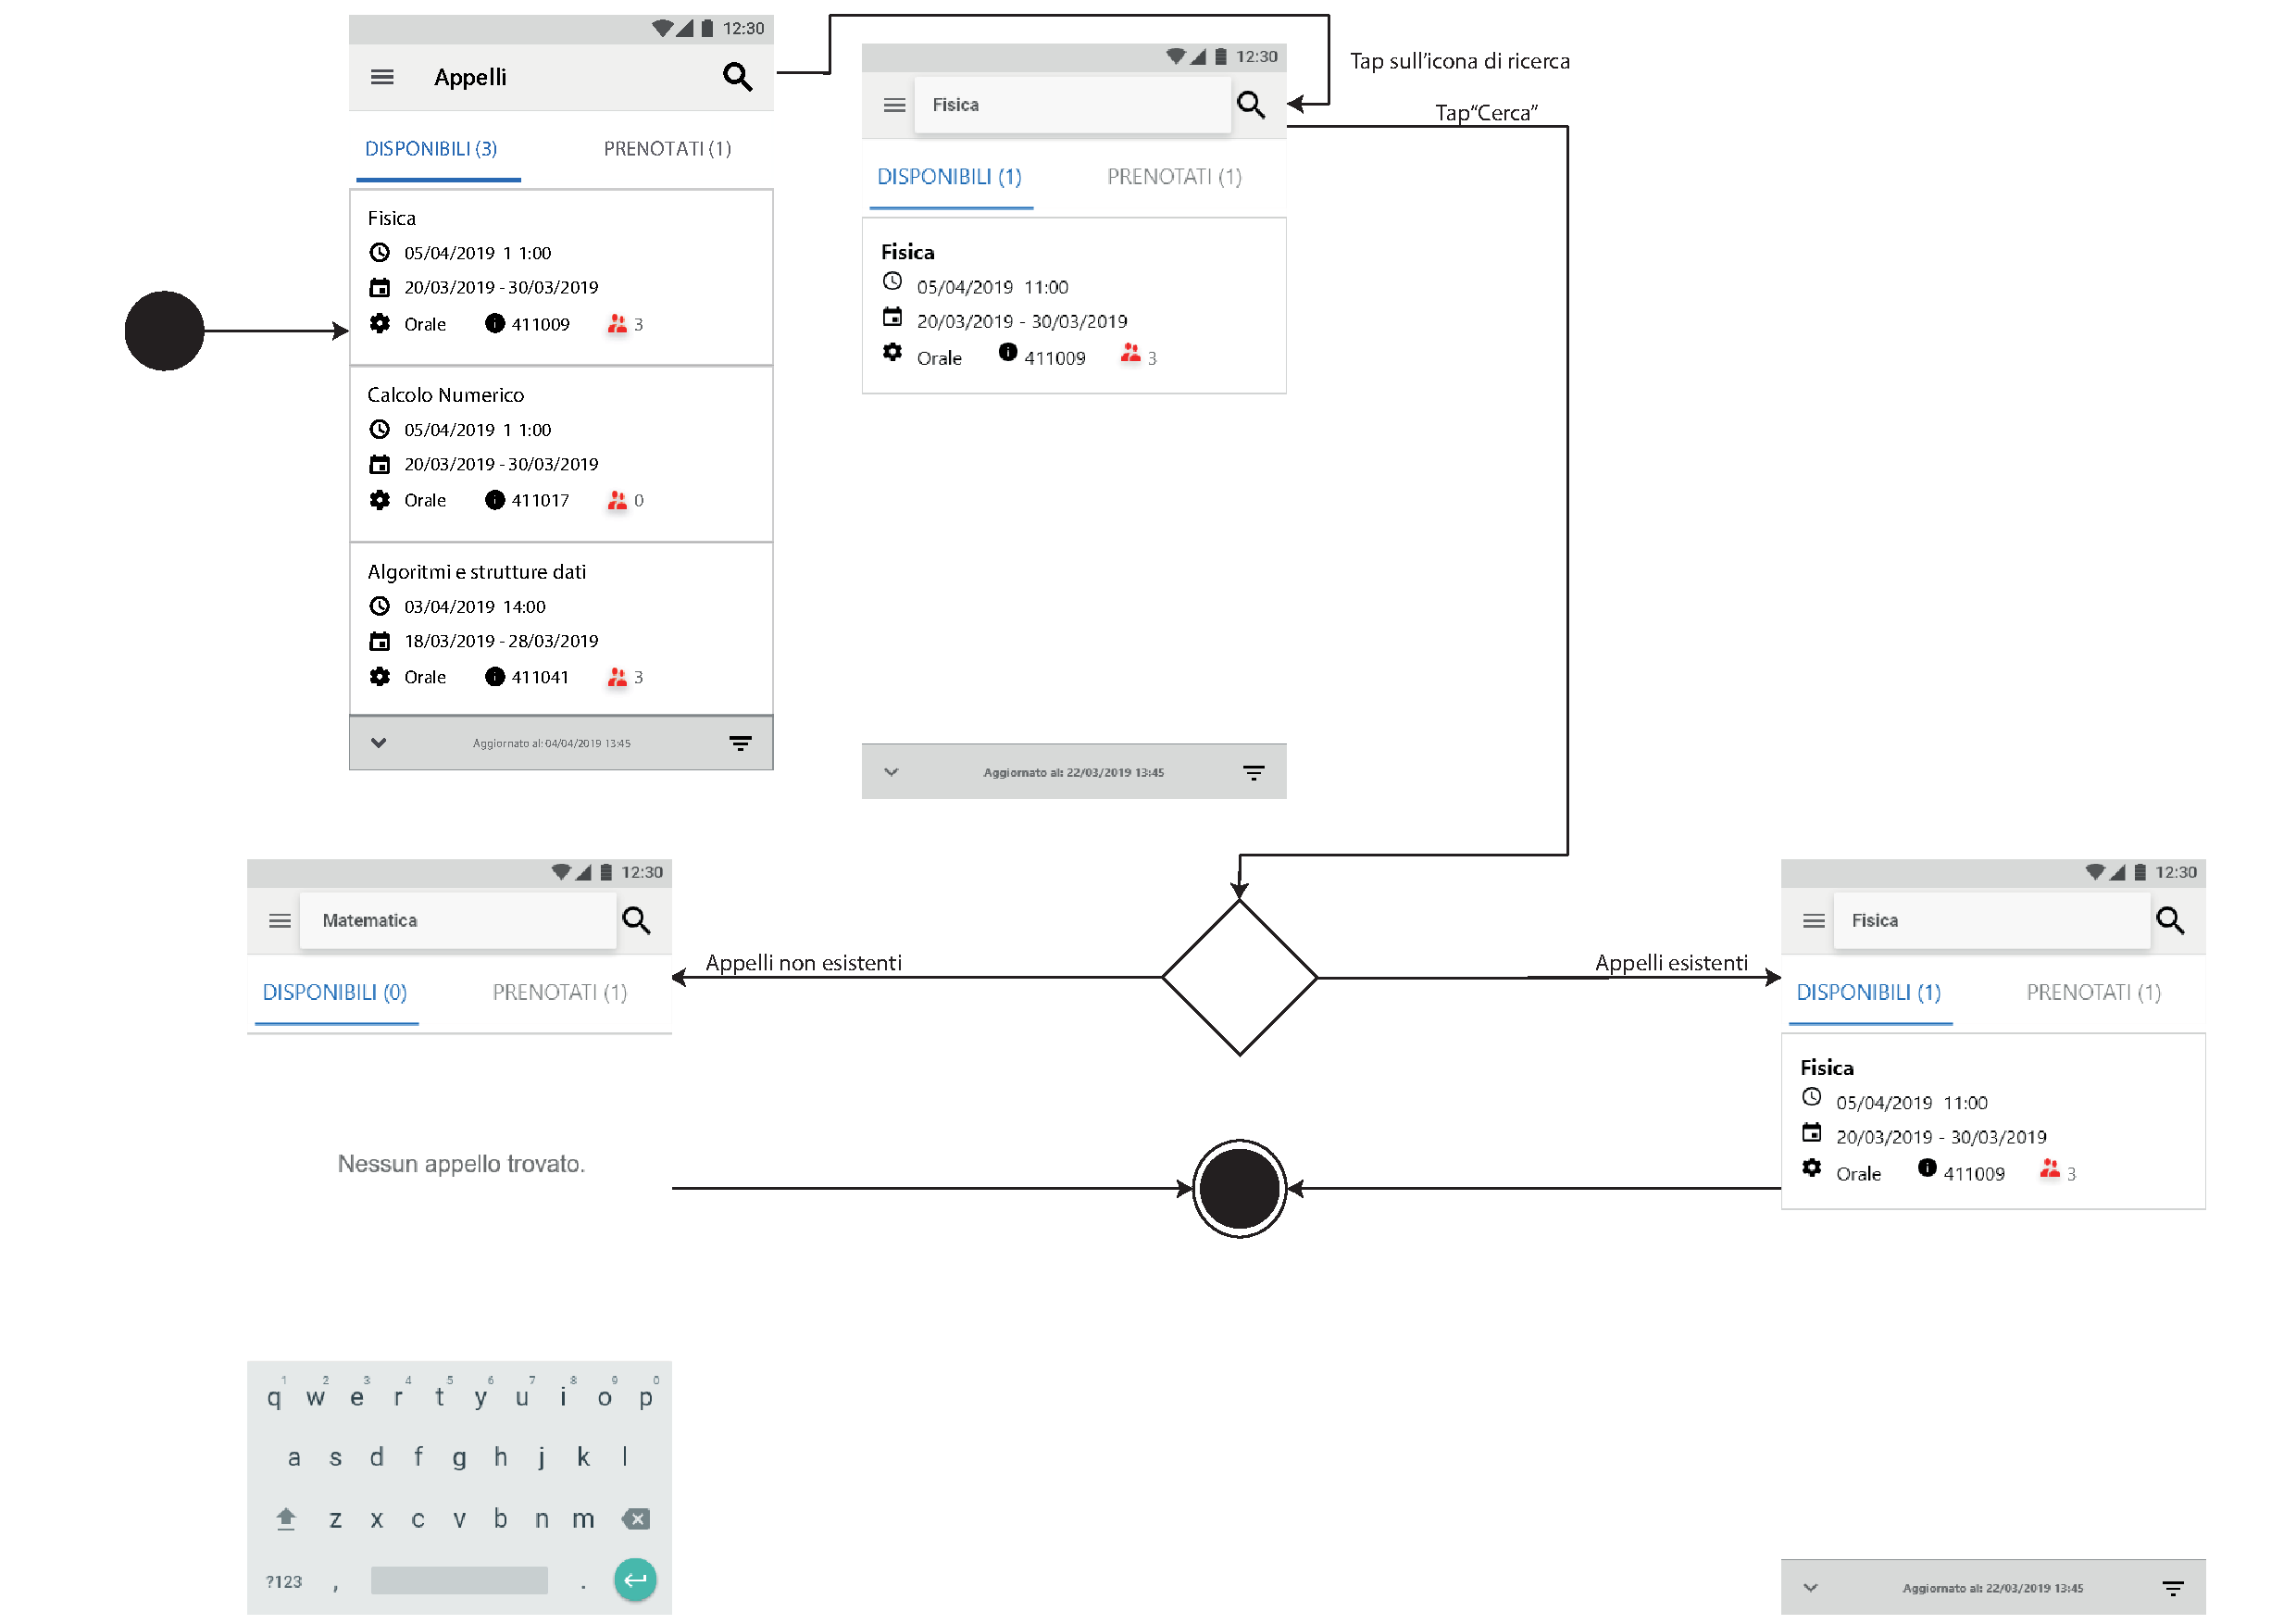
\includegraphics[width=6in]{imgs/gruppo1/activity_diagrams/AD8_Ricerca_appelli.pdf}
	\caption{Activity Diagram - Ricerca appelli disponibili}
	\label{diag:ricercaAppelliDisponibiliAD}
\end{figure}
\newpage

%\paragraph{Filtra appelli disponibili con memorizzazione }
\begin{figure}
	\centering
	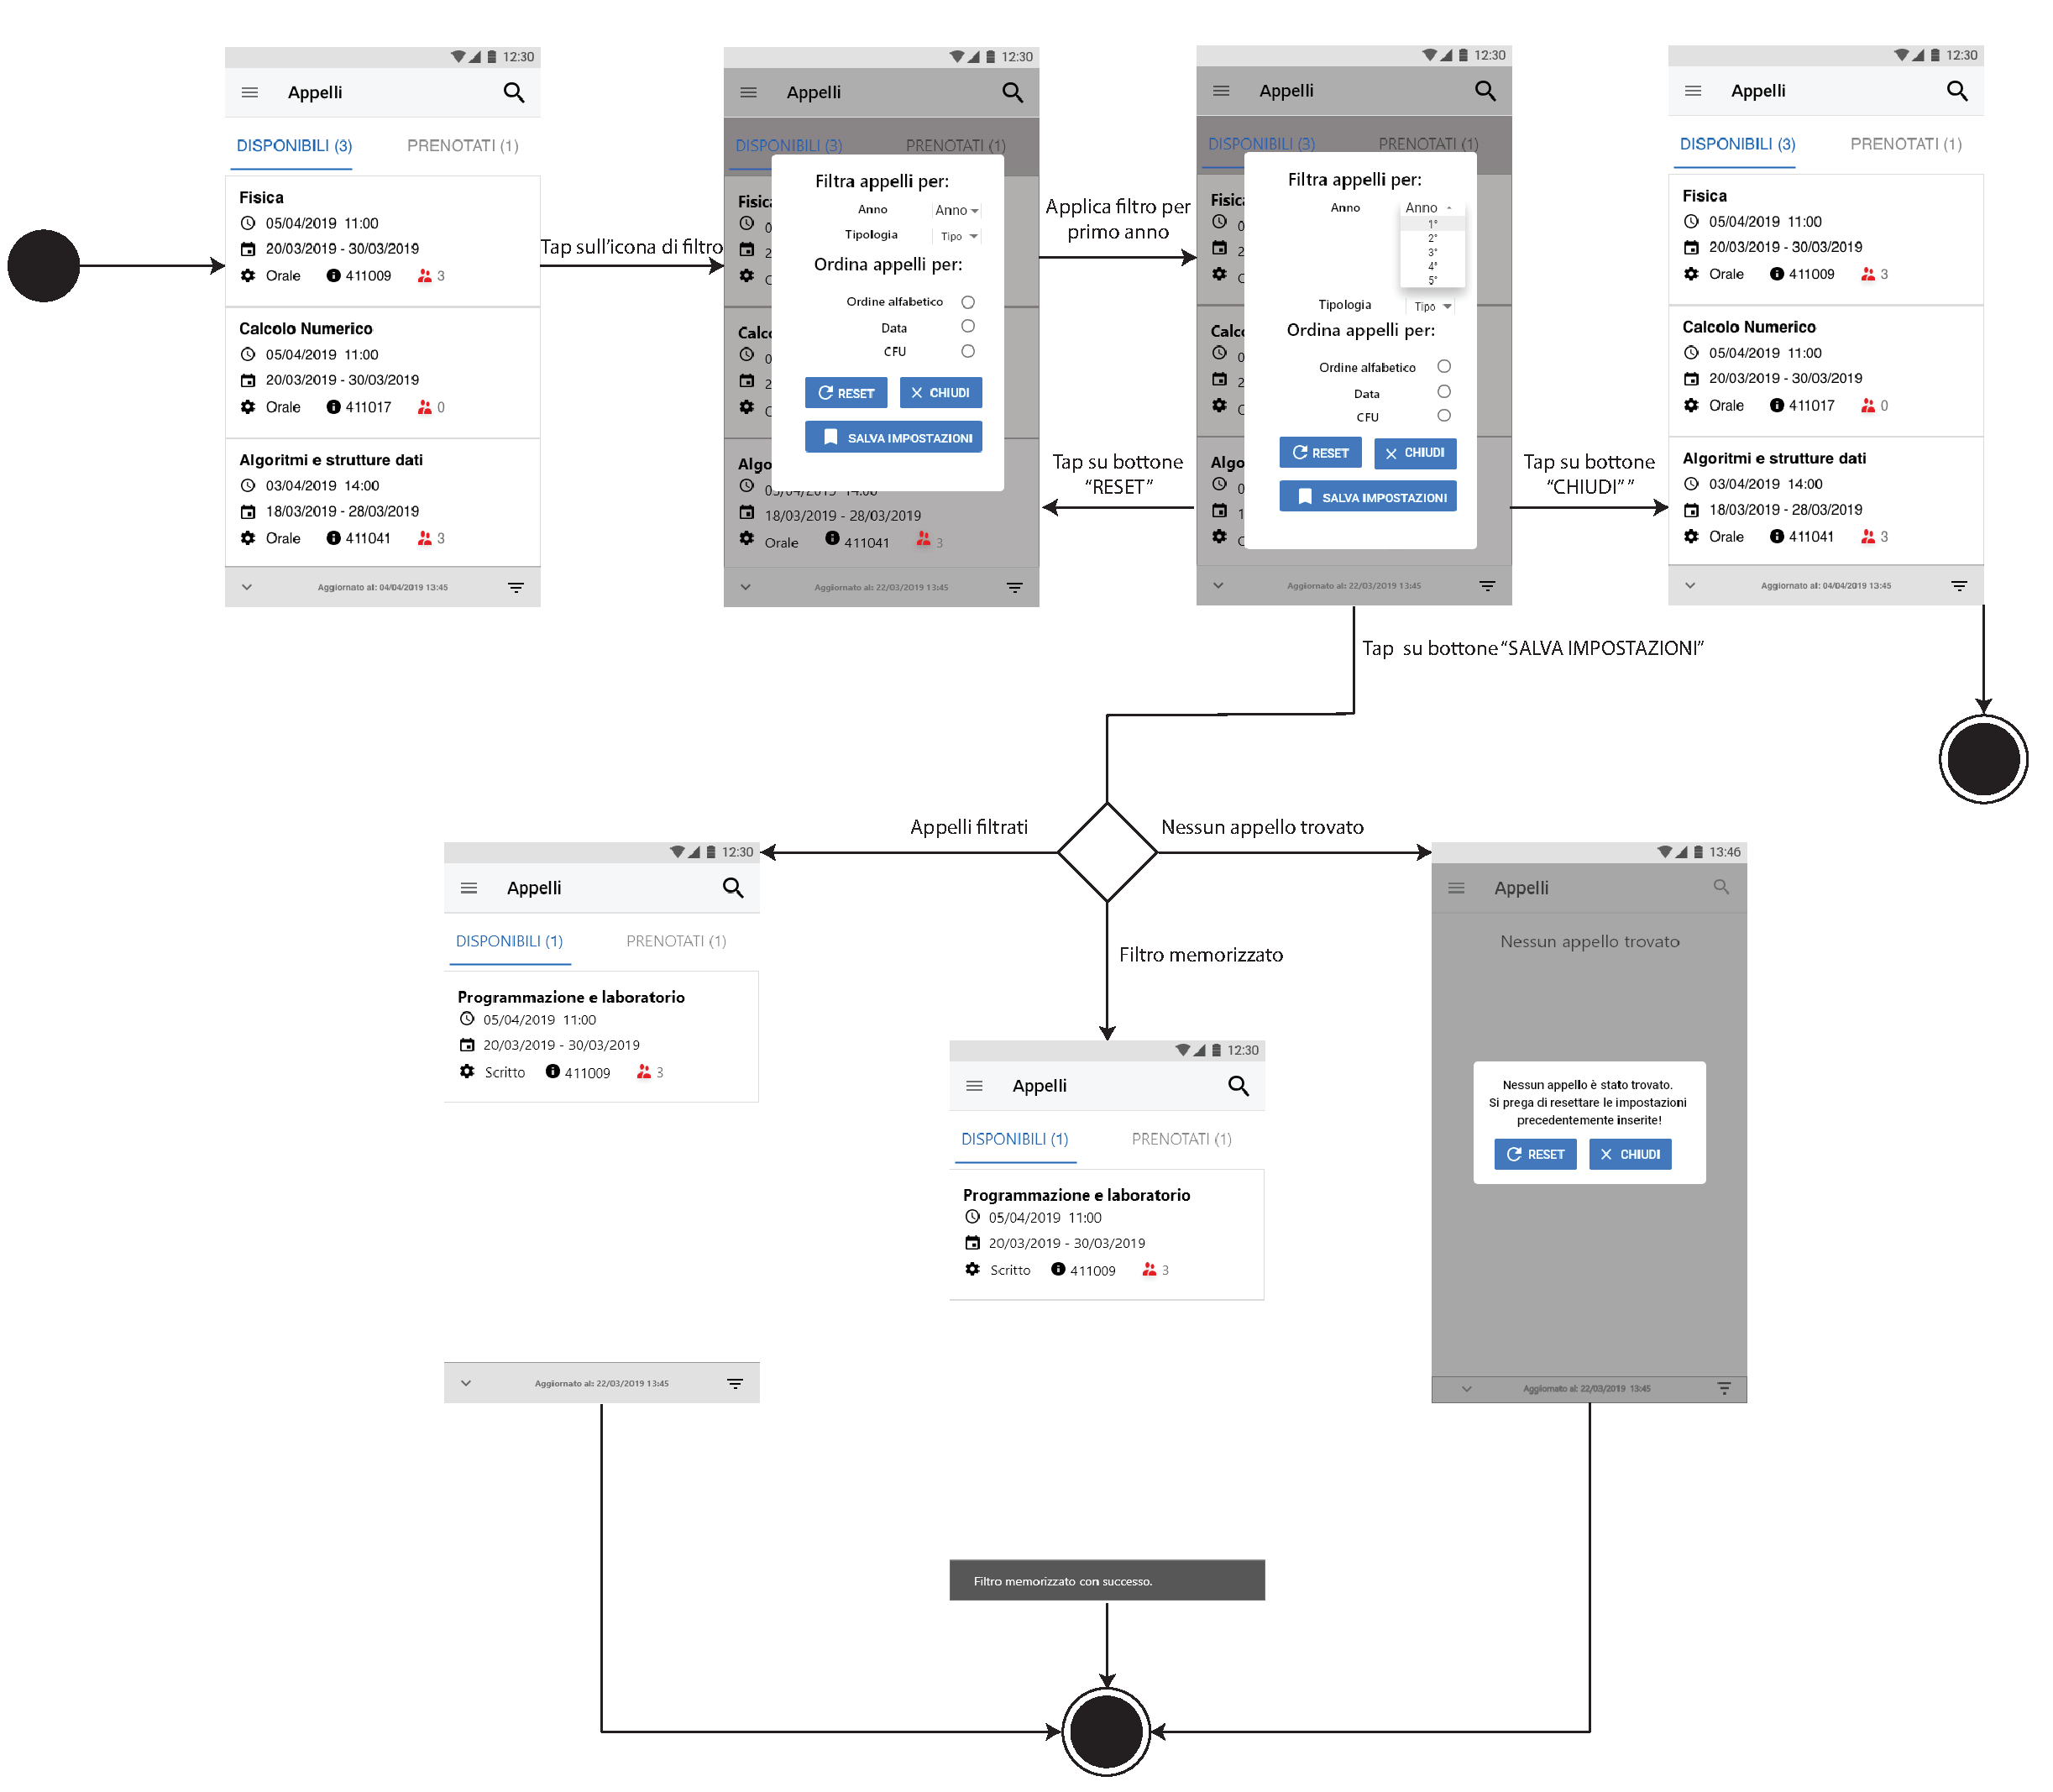
\includegraphics[width=6in]{imgs/gruppo1/activity_diagrams/AD9_filtrati_appelli.pdf}
	\caption{Activity Diagram - Filtra appelli disponibili con memorizzazione}
	\label{diag:filtraAppelliDisponibiliConMemAD}
\end{figure}
\newpage

%\paragraph{Ordina appelli disponibili con memorizzazione }
\begin{figure}
	\centering
	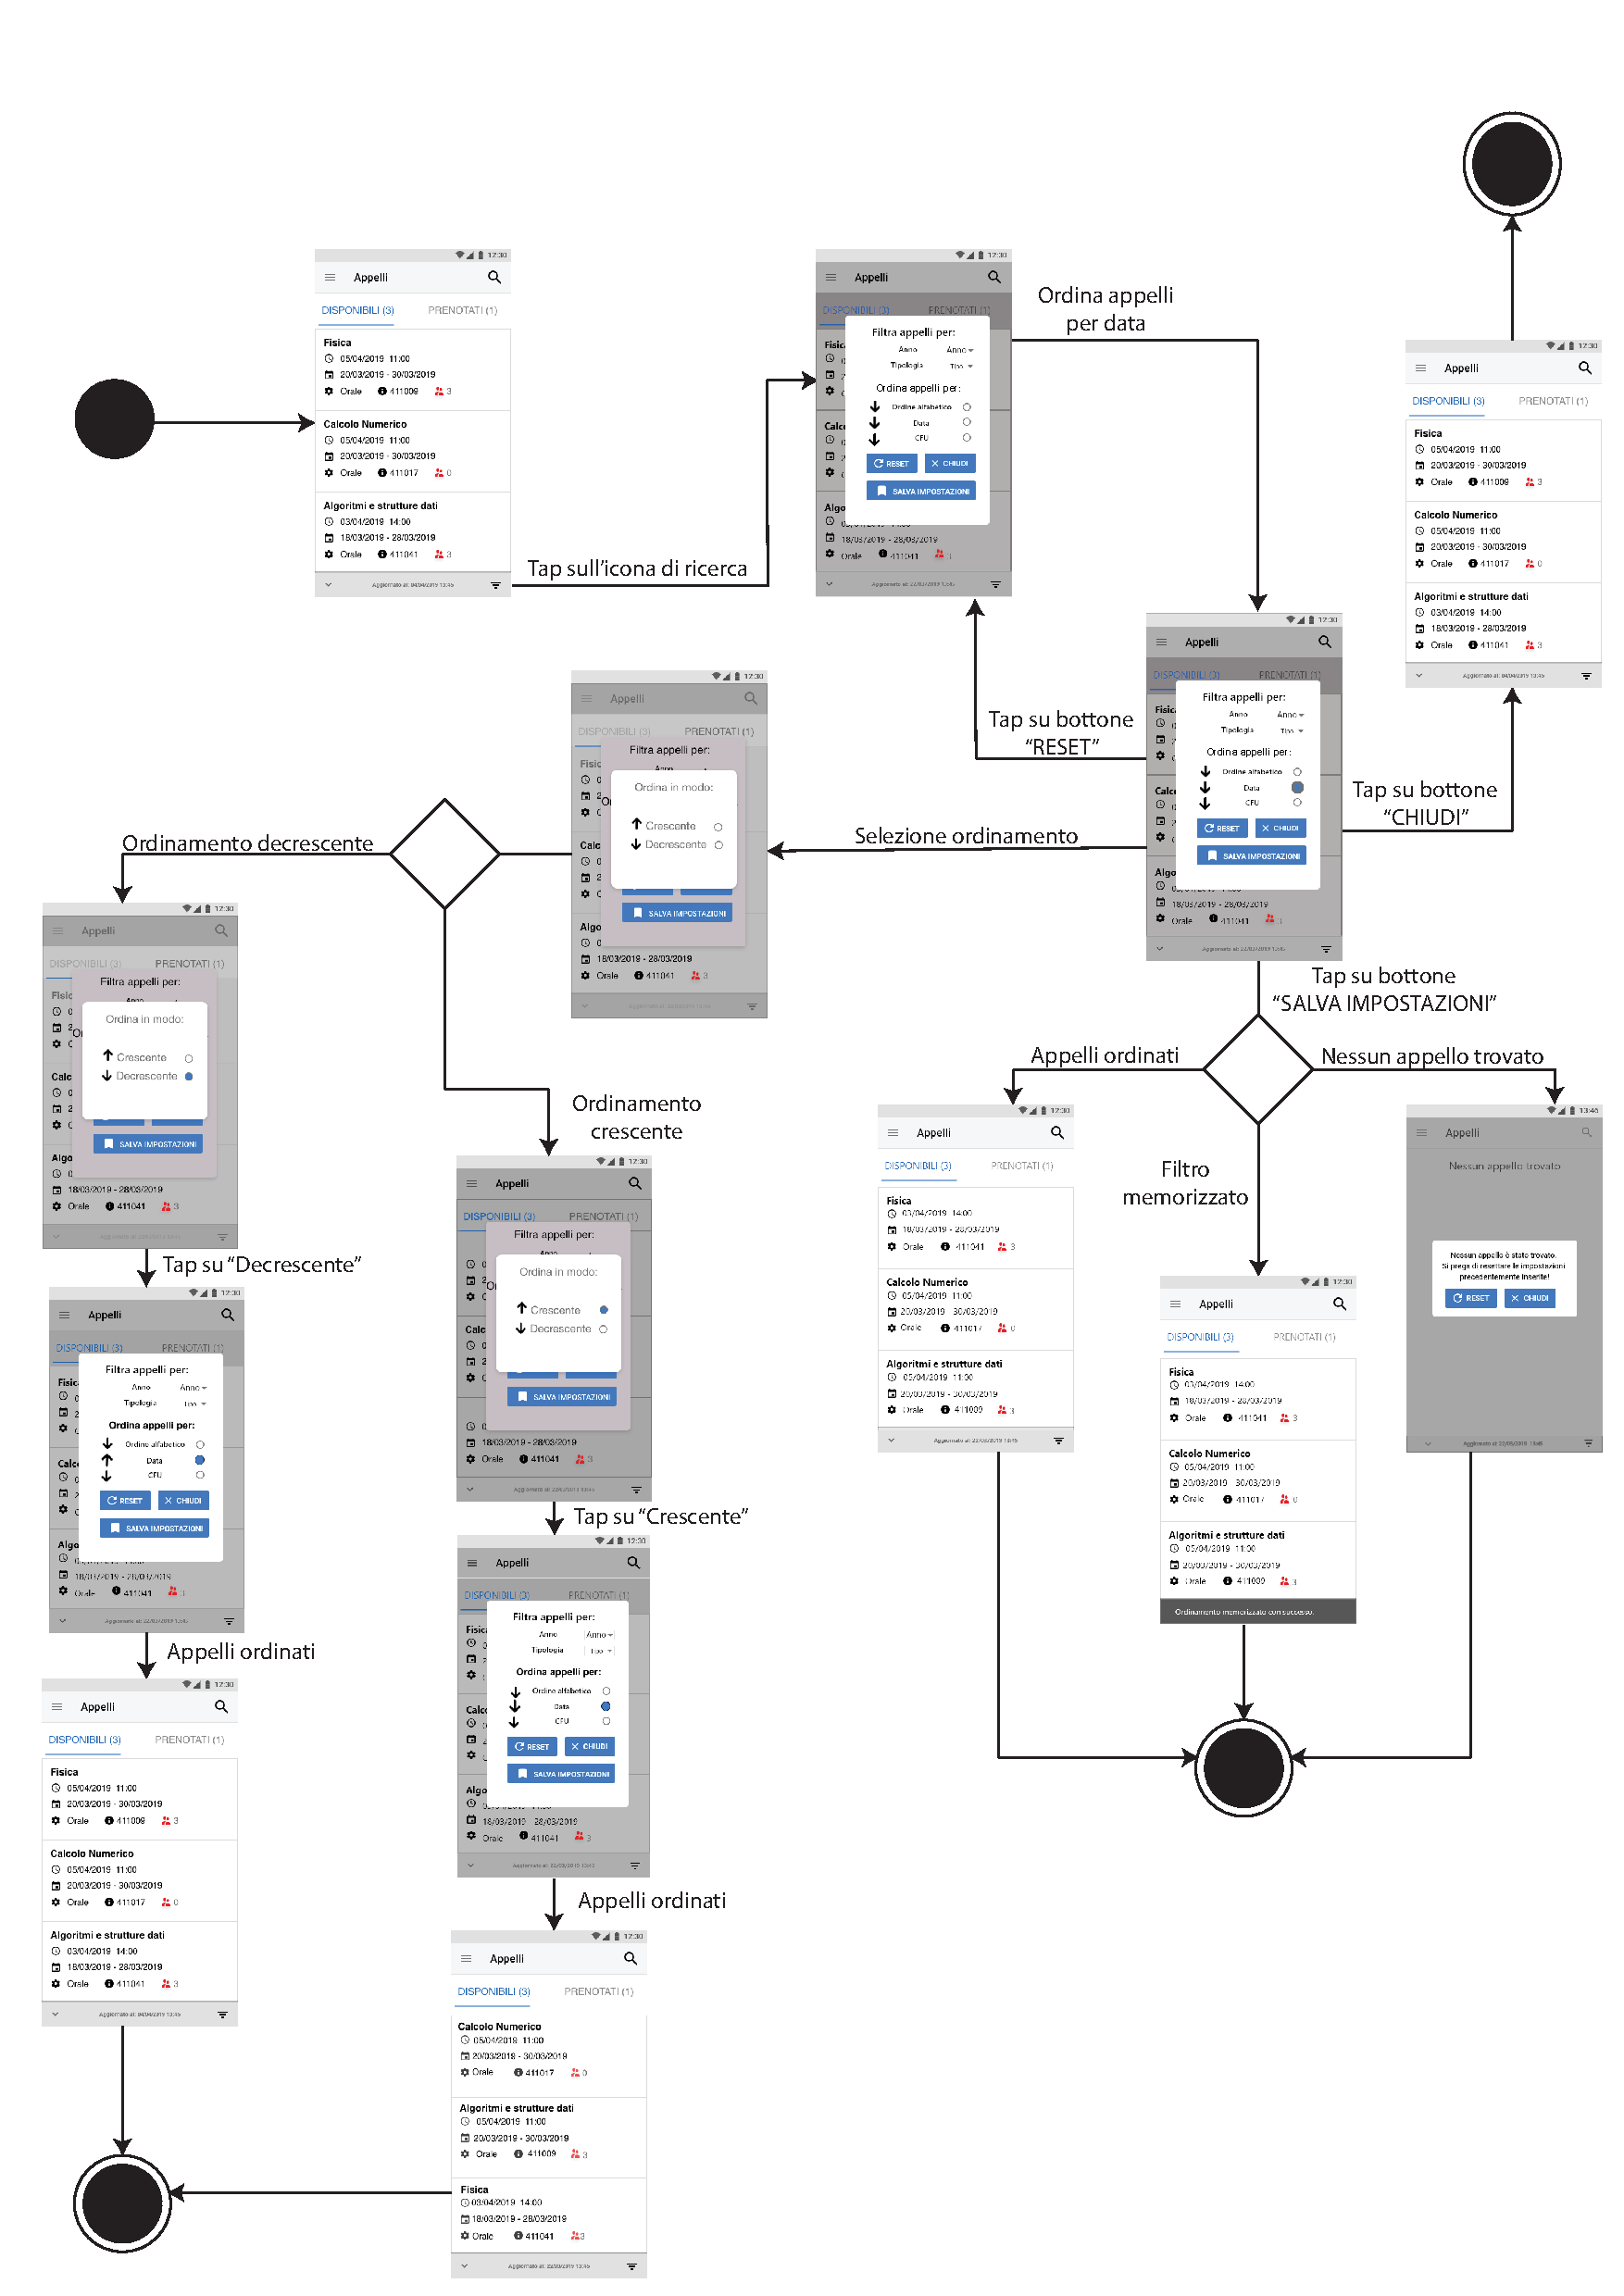
\includegraphics[width=6in]{imgs/gruppo1/activity_diagrams/AD10_ordina_appelli.pdf}
	\caption{Activity Diagram - Ordina appelli disponibili con memorizzazione}
	\label{diag:ordinaAppelliDisponibiliConMemAD}
\end{figure}
\newpage

%\paragraph{Prenota appello }
\begin{figure}
	\centering
	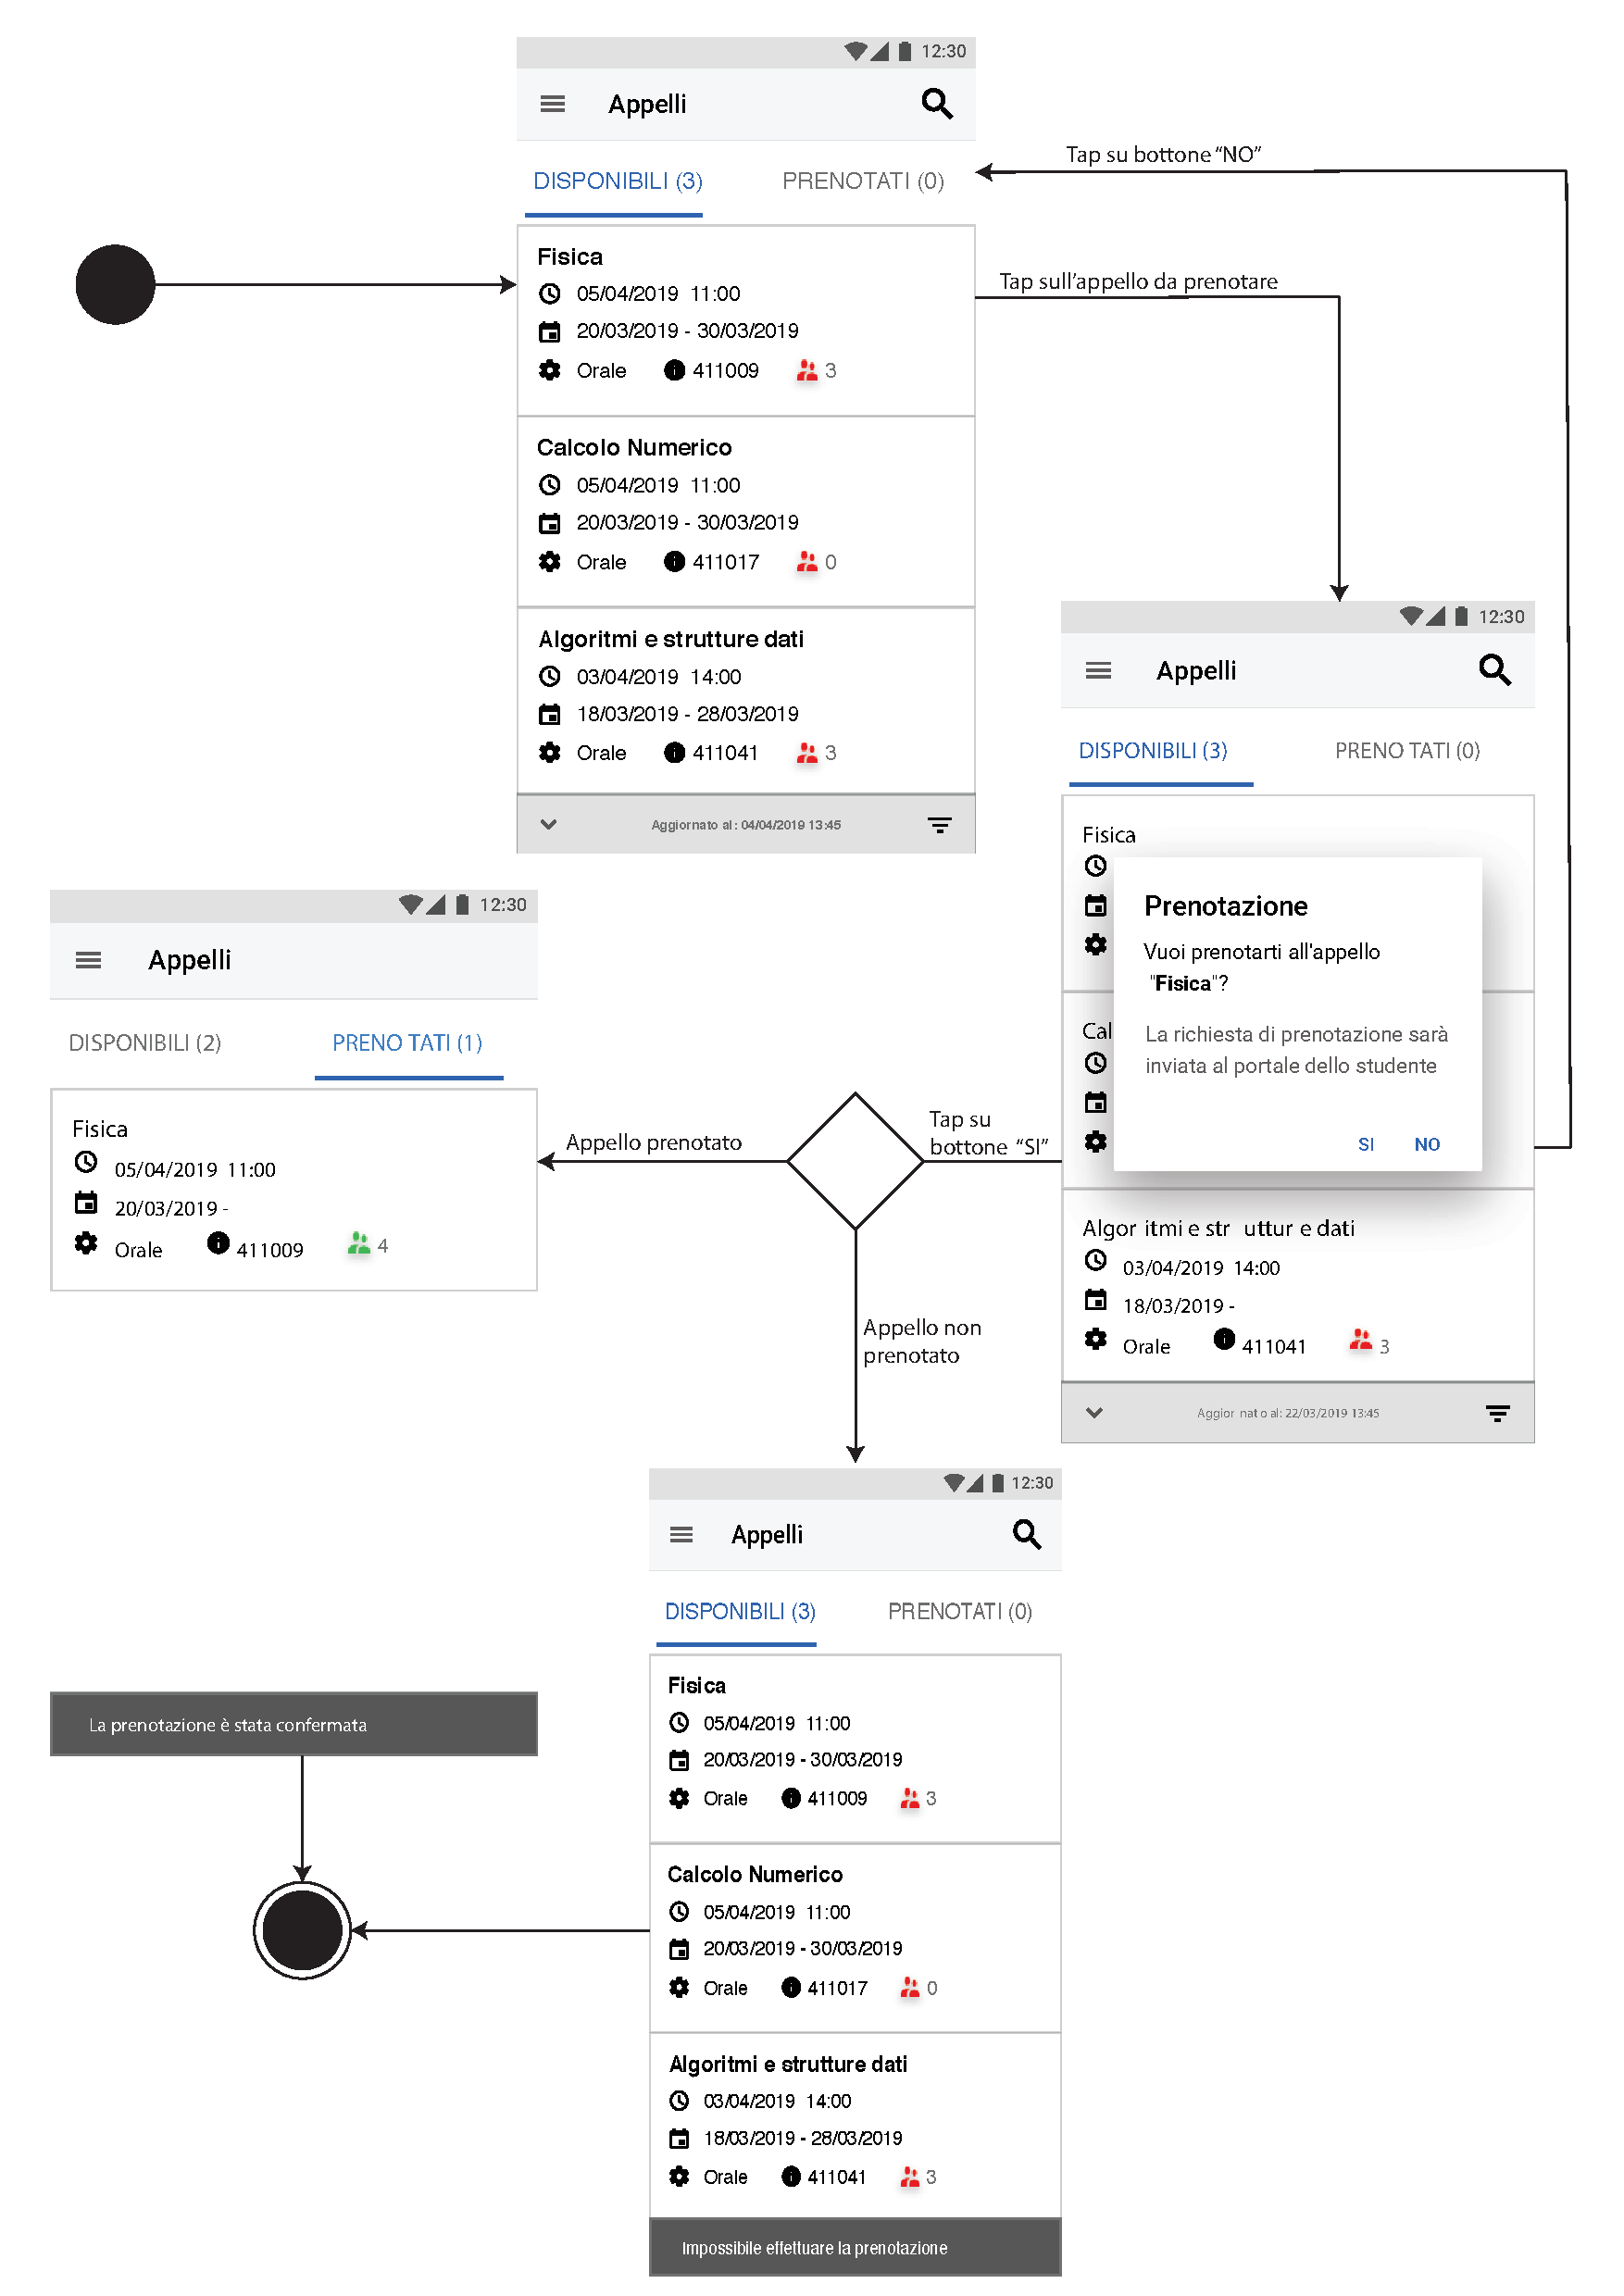
\includegraphics[width=6in]{imgs/gruppo1/activity_diagrams/AD11_prenota_apppello.pdf}
	\caption{Activity Diagram - Prenota appello}
	\label{diag:prenotaAppelloAD}
\end{figure}
\newpage

%\paragraph{Cancella prenotazione}
\begin{figure}
	\centering
	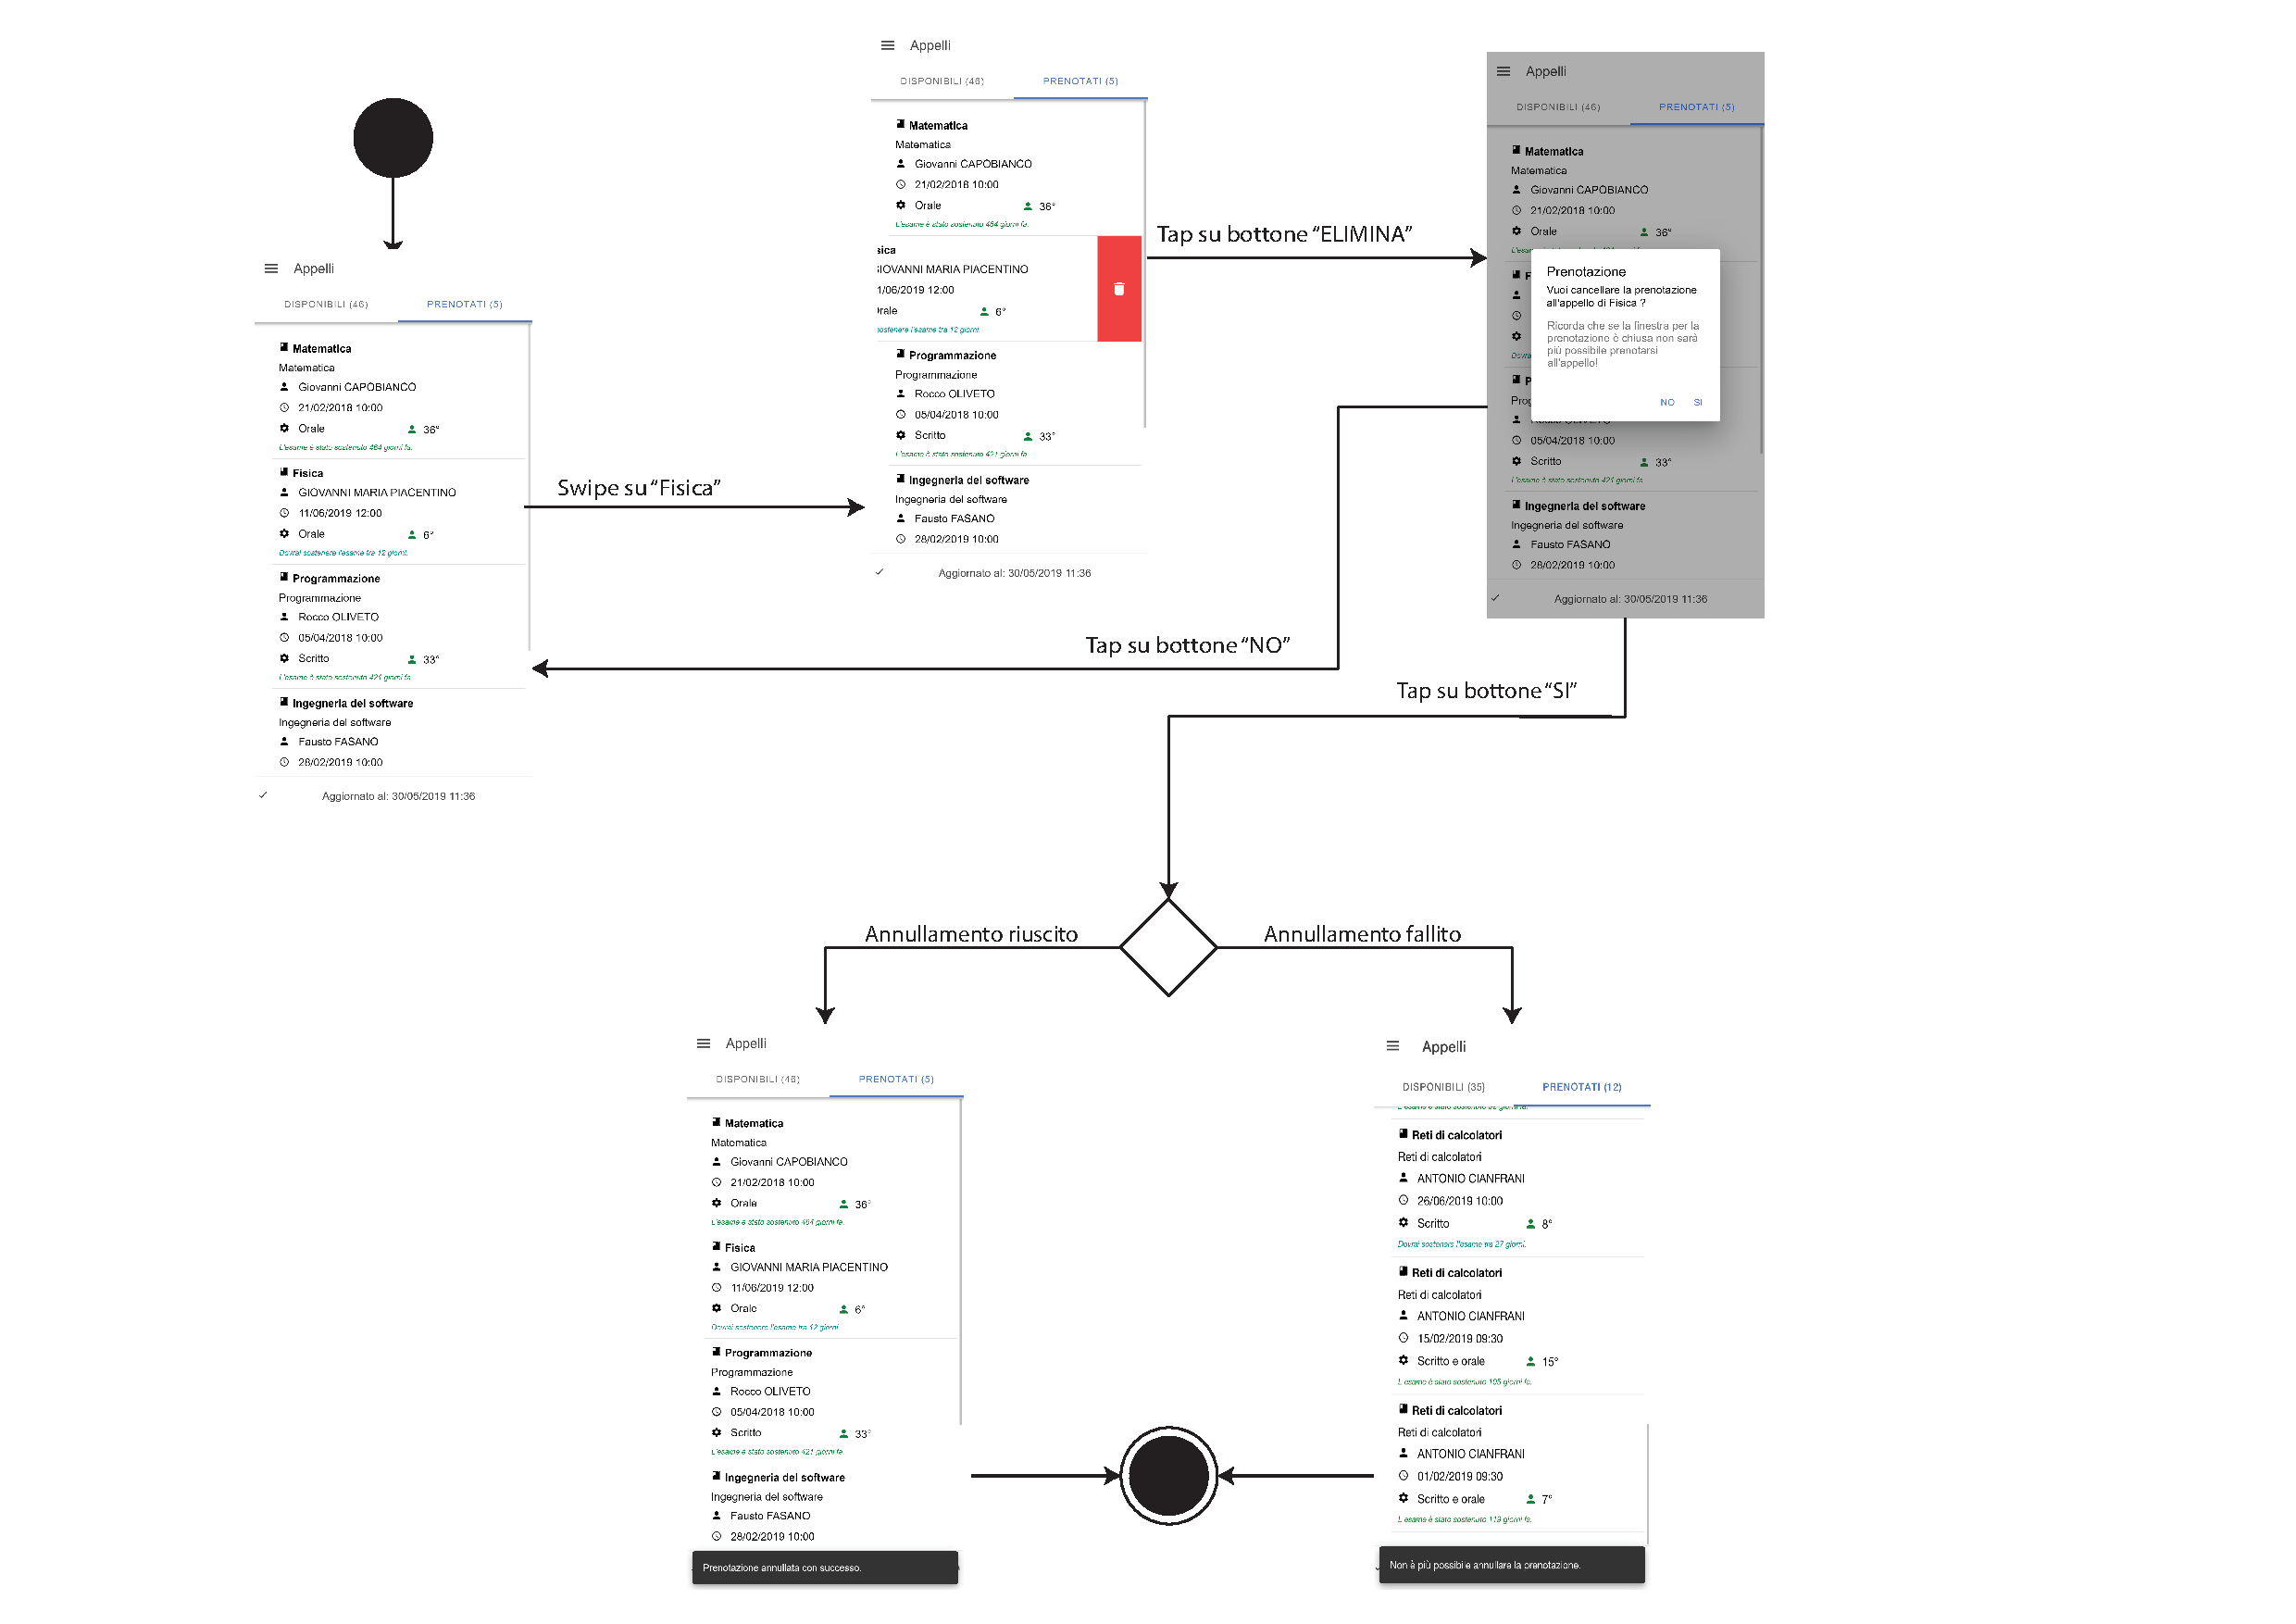
\includegraphics[width=6in]{imgs/gruppo1/activity_diagrams/AD12_cancella_prenotazione.pdf}
<<<<<<< HEAD
	\caption{Activity Diagram - Cancella Prenotazione}
	\label{diag:cancellaPrenotazioneAD}
\end{figure}

\clearpage
\subsection{Funzionalità Gestione materiale didattico}

%\paragraph{Visualizza elenco file}
\begin{figure}
	\centering
	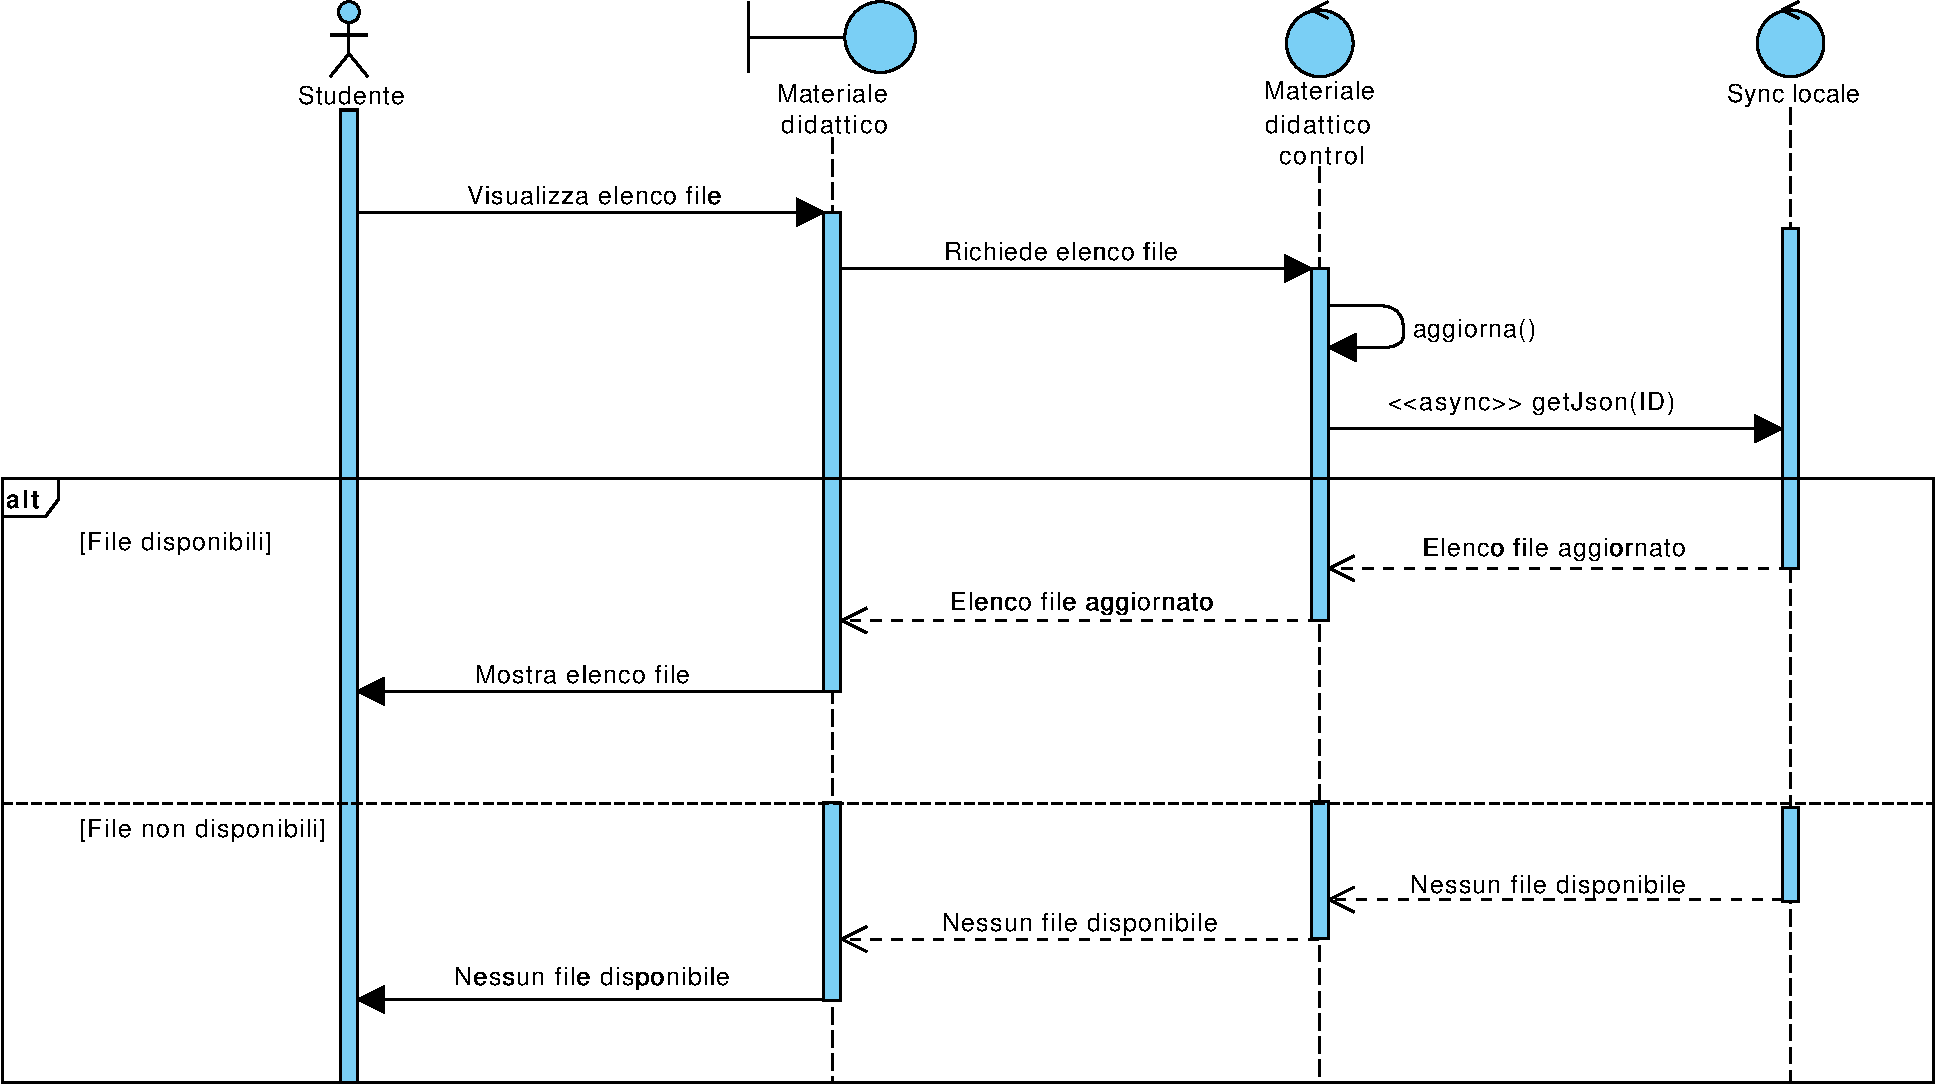
\includegraphics[width=6.5in]{imgs/gruppo1/sequence_diagrams/SD13_visualizza_elenco_file.pdf}
	\caption{Sequence Diagram - Visualizza elenco file}
	\label{diag:visualizzaElencoFileSD}
\end{figure}

%% 8.5.14 - Ricerca file %
\paragraph{Ricerca file}
\begin{figure}
	\centering
	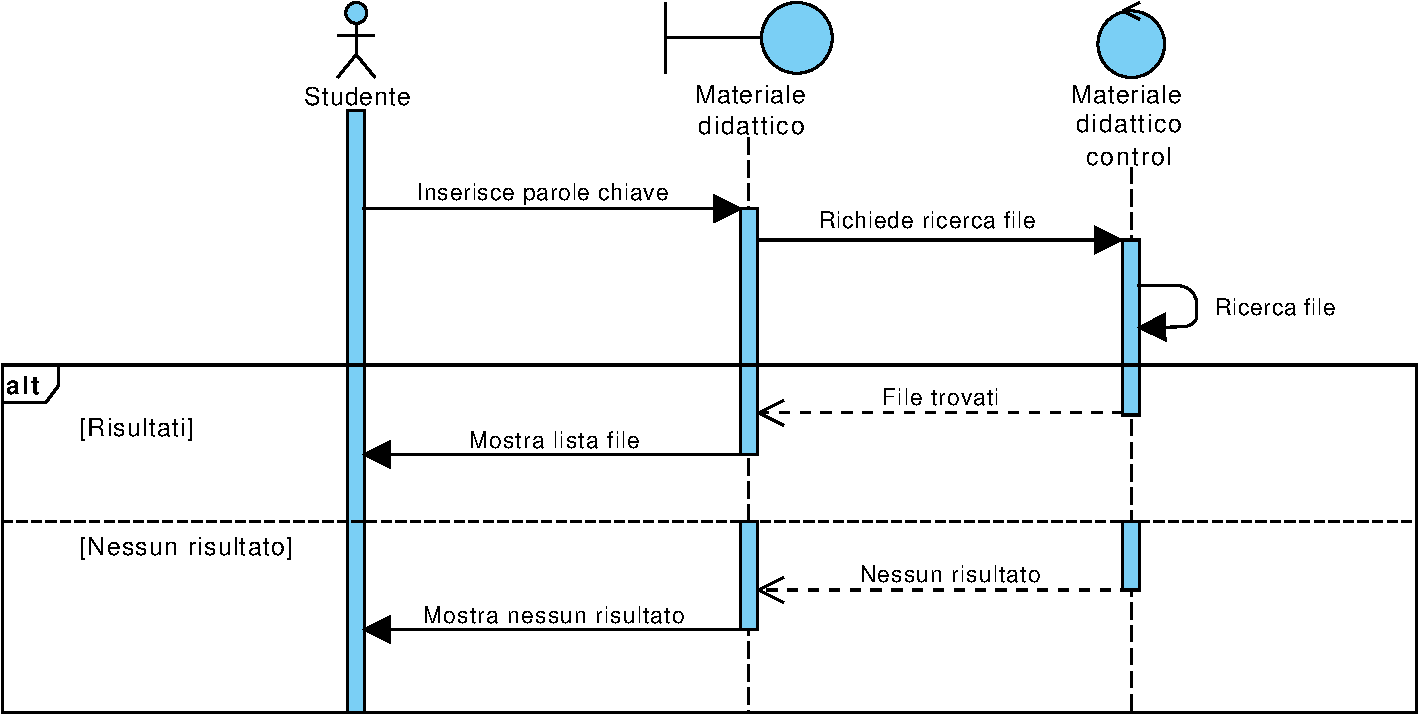
\includegraphics[width=6.5in]{imgs/gruppo1/sequence_diagrams/SD14_ricerca_file.pdf}
	\caption{Sequence Diagram - Ricerca file}
	\label{diag:ricercaFileSD}
\end{figure}
\newpage

%\paragraph{Visualizza dettagli file}
\begin{figure}
	\centering
	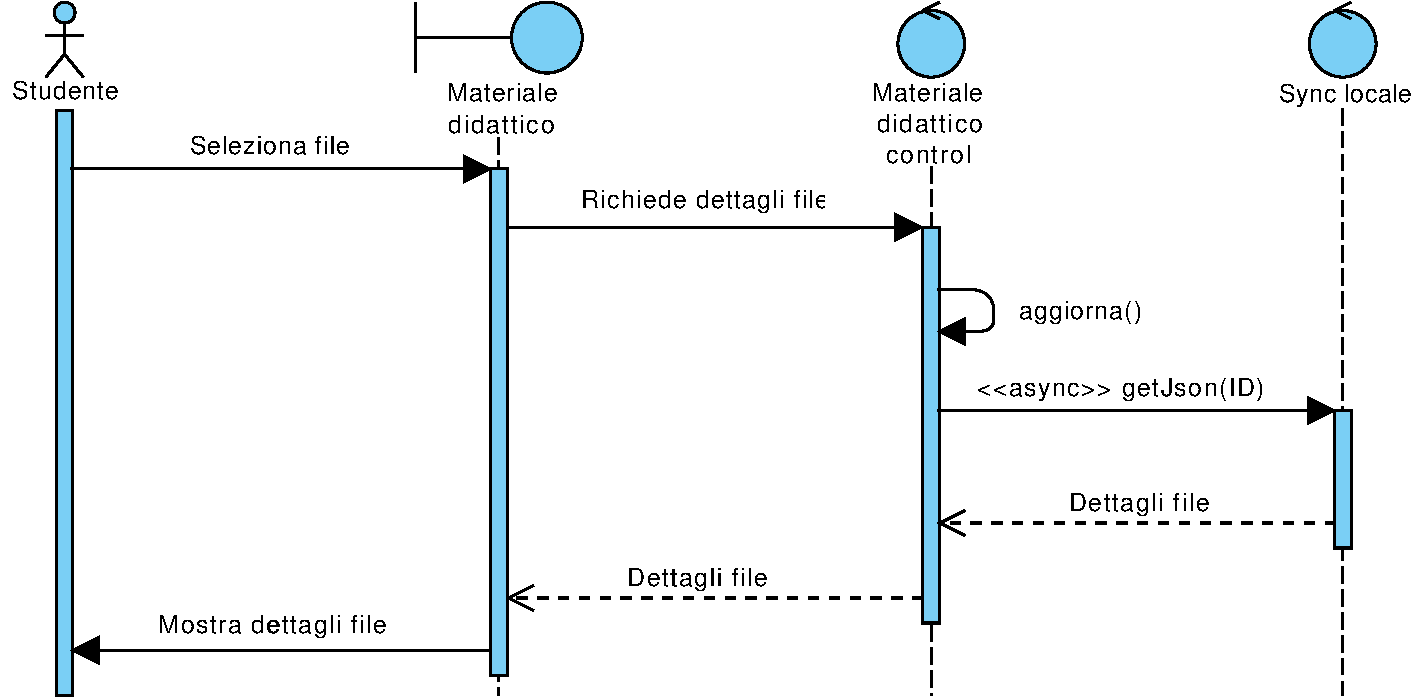
\includegraphics[width=6.5in]{imgs/gruppo1//sequence_diagrams/SD15_visualizza_dettagli_file.pdf}
	\caption{Sequence Diagram - Visualizza dettagli file}
	\label{diag:visualizzaDettagliFileSD}
\end{figure}

%\paragraph{Apri file}
\begin{figure}
	\centering
	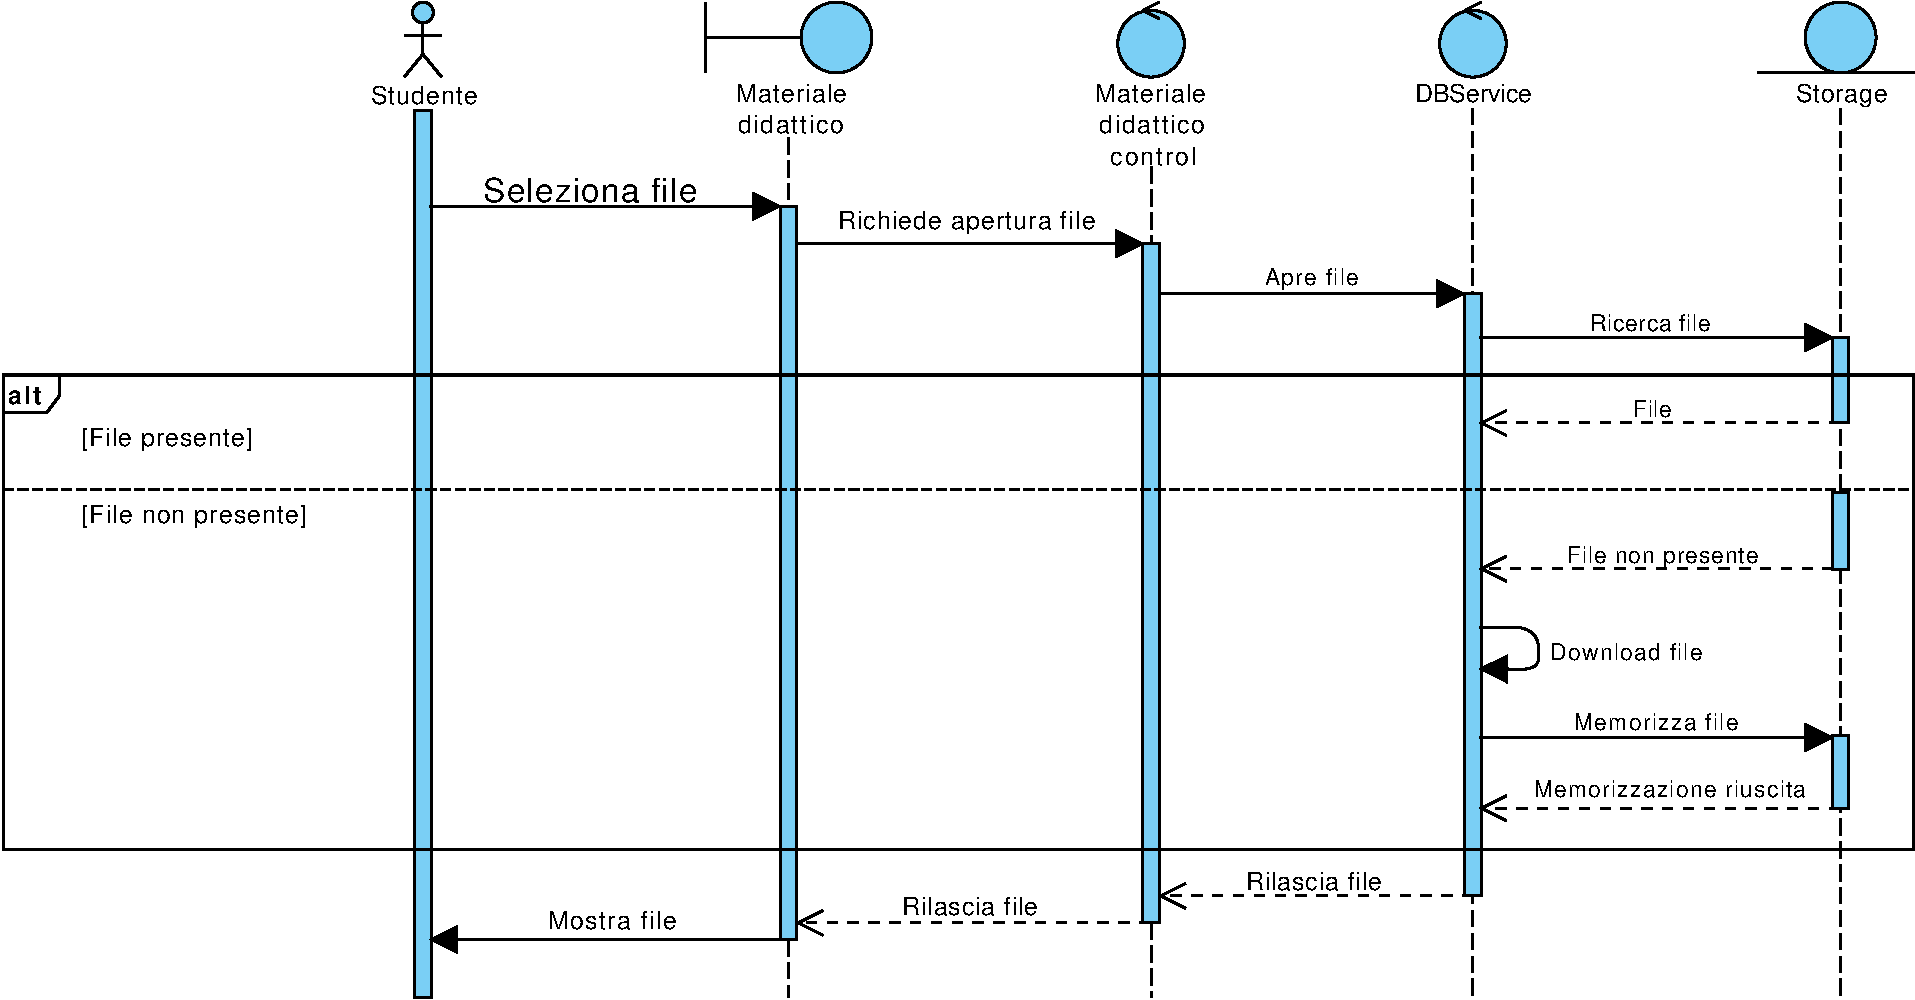
\includegraphics[width=6.5in]{imgs/gruppo1/sequence_diagrams/SD16_apri_file.pdf}
	\caption{Sequence Diagram - Apri file}
	\label{diag:apriFileSD}
\end{figure}
\newpage

%\paragraph{Rimuovi  file}
\begin{figure}
	\centering
	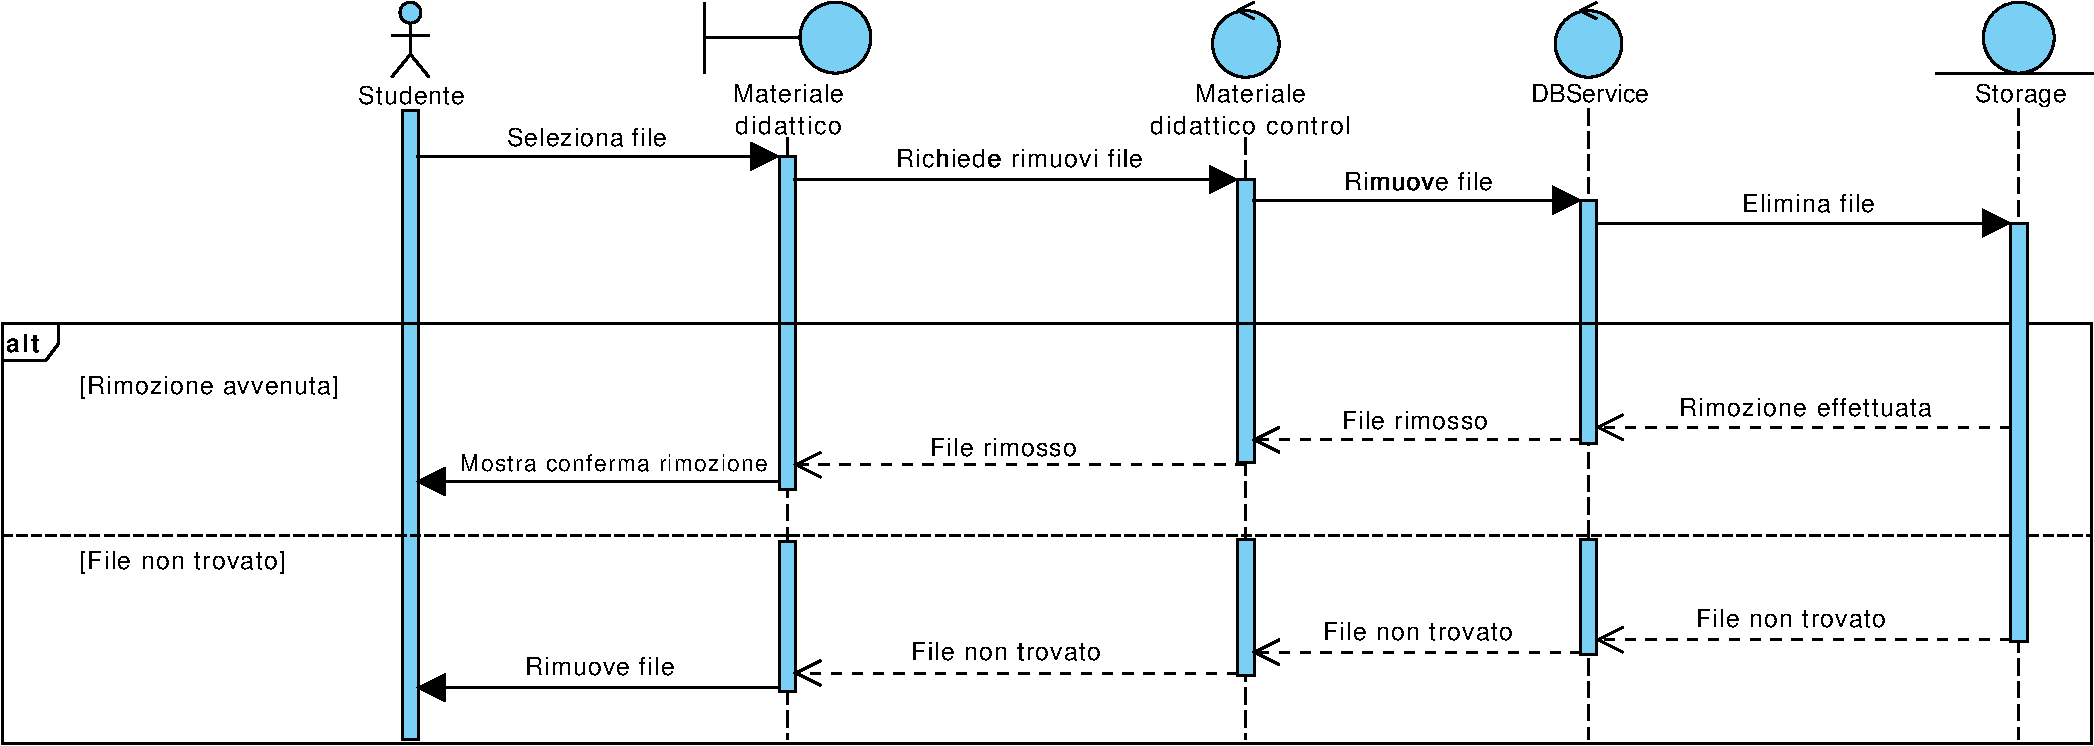
\includegraphics[width=6.5in]{imgs/gruppo1/sequence_diagrams/SD17_rimuovi_file.pdf}
	\caption{Sequence Diagram - Rimuovi file}
	\label{diag:rimuoviFileSD}
\end{figure}

\clearpage
\subsection{Funzionalità orario}

\subsubsection{Gestione primo avvio}

Giulio, dopo aver selezionato la sezione “orario” dalla voce del menu, potrà spuntare, da una lista di corsi, quelli che vuole seguire. Confermerà la selezione premendo l’apposito tasto “OK”. Da questo momento in poi Giulio potrà visualizzare l’orario costituito dai corsi scelti. 

\subsubsection{Modifica orario}

Giulio modificherà l’orario del proprio anno accademico spuntando la lista dei corsi che vuole seguire. Una volta confermata la modifica, lo studente visualizzerà l’orario aggiornato. 

\subsubsection{Visualizza orario}

Dopo il primo avvio dell’orario, selezionando la sezione “orario” dalla voce del menu, Giulio visualizzerà l’orario.
\subsection{Funzionalità notifiche}

Diagramma di sequenza: Vedi Figura~\vref{fig:seq-diagr-notifiche}.

\begin{figure}
	\centering
	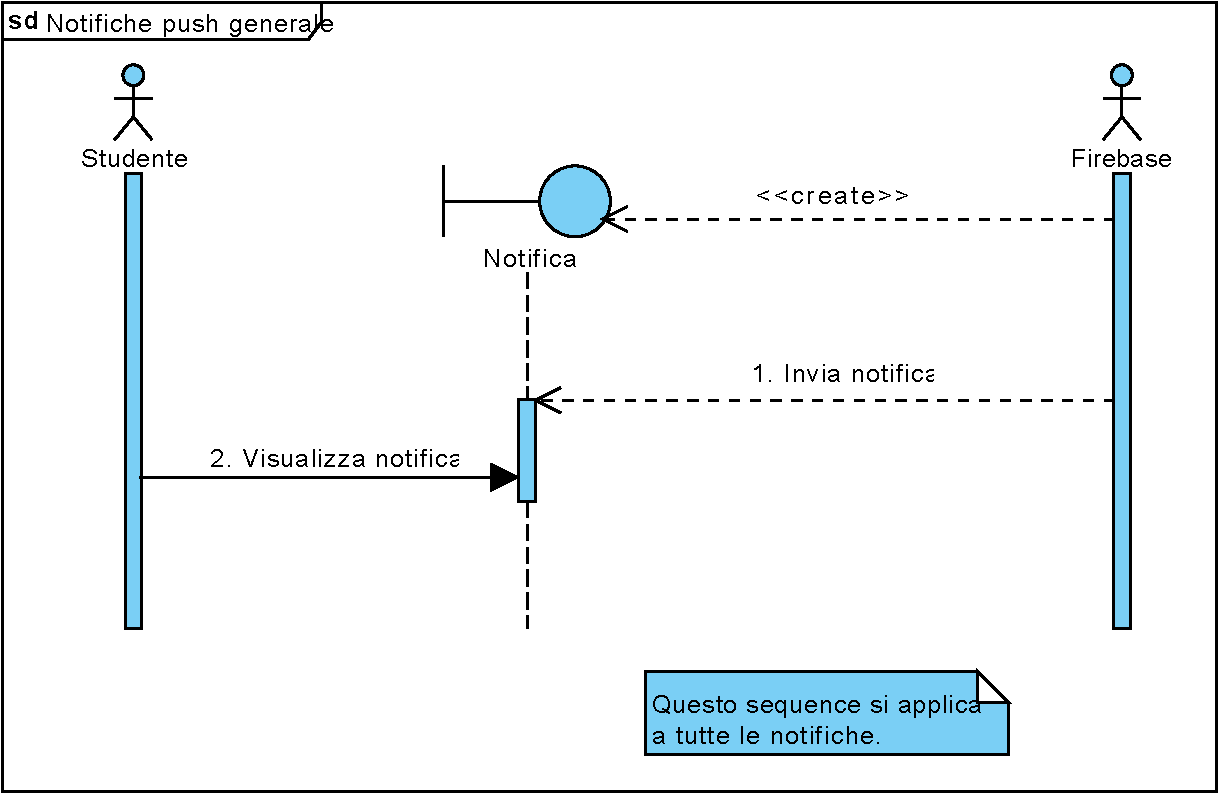
\includegraphics[width=0.85\textwidth]{imgs/gruppo2/sequence-notifiche}
	\caption{Sequence diagram - Notifiche}
	\label{fig:seq-diagr-notifiche}
\end{figure}

\clearpage
\subsection{Funzionalità chat}

\paragraph{CUS1 - Visualizza canale \\}

Lo \emph{Studente}, una volta selezionata la voce \emph{“chat”} dal \emph{menù} dell’app \emph{Studenti Unimol},  seleziona una \emph{chat} specifica della lista e visualizza i messaggi presenti nel canale di discussione della stessa. Nel caso in cui vi sia l’assenza di connessione viene visualizzata l’ultima copia salvata in locale del canale qualora essa sia presente.
\begin{table}
	\small % Dimensione testo piccola
	\label{CUS1 - Visualizza canale}
	\begin{tabular}{| p{\useCaseLeft} | p{\useCaseNum} | p{\useCaseTwoCol} | p{\useCaseTwoCol} |}
		\hline
		\textbf{Nome caso d'uso} & \multicolumn{3}{p{\useCaseMulticol} |}{\textbf{CUS 1 - Visualizza canale}} \\
		\hline
		\textbf{Attori partecipanti} & \multicolumn{3}{p{\useCaseMulticol} |}{Inizializzato da \textbf{\emph{Studente}.}} \\
		\hline
		\textbf{Condizioni d'ingresso} & \multicolumn{3}{p{\useCaseMulticol} |}{Lo \emph{Studente} seleziona la voce \emph{“chat”} dal \emph{menù} dell’\emph{app Studenti Unimol}.} \\
		\hline
		\textbf{Flusso degli eventi} & \textbf{\#} & \textbf{\emph{Studente}} & \textbf{Sistema} \\
		\hline
		\textbf{} & \textbf{1} & \textbf{} & Mostra l’\emph{home-chat} con le relative \emph{chat}; \\
		\hline
		\textbf{} & \textbf{2} & Seleziona la \emph{chat} desiderata; & \textbf{} \\
		\hline
		\textbf{} & \textbf{3} & \textbf{} & Mostra il canale di discussione di \emph{default} della \emph{chat}; \\
		\hline
		\textbf{} & \textbf{4} & Seleziona un canale di discussione alternativo; & \\
		\hline
		\textbf{} & \textbf{5} & \textbf{} & Mostra il canale di discussione selezionato; \\
		\hline
		\textbf{Eccezioni} & \multicolumn{3}{p{\useCaseMulticol} |}{1.1 - 3.1 - 5.1 Nessuna risposta dal \emph{server}: viene visualizzato un messaggio di errore; \newline1.2 - 3.2 - 5.2  Connessione assente: il sistema restituisce l’ultima copia salvata in locale; \newline 1.3 - 3.3 - 5.3 Copia non presente: viene visualizzato un messaggio di errore;} \\
		\hline
		\textbf{Condizioni d'uscita} & \multicolumn{3}{p{\useCaseMulticol} |}{Lo \emph{Studente} visualizza il canale correttamente.} \\
		\hline
	\end{tabular}
	\caption{CUS1 - Visualizza canale}
\end{table}

\newpage
	\paragraph{CUS2 - Invio messaggio \\}

Lo \emph{Studente}, all’interno di un canale di discussione, invia un messaggio selezionando l’apposito spazio dedito alla scrittura. Una volta digitato il testo del messaggio e selezionato il pulsante di invio, il sistema lo mostra nel canale di discussione. \\
\begin{table}

	\small % Dimensione testo piccola
	\label{CUS2 - Invio messaggio}
	\begin{tabular}{| p{\useCaseLeft} | p{\useCaseNum} | p{\useCaseTwoCol} | p{\useCaseTwoCol} |}
		\hline
		\textbf{Nome caso d'uso} & \multicolumn{3}{p{\useCaseMulticol} |}{\textbf{CUS2 - Invio messaggio}} \\
		\hline
		\textbf{Attori partecipanti} & \multicolumn{3}{p{\useCaseMulticol} |}{Inizializzato da \textbf{\emph{Studente}.}} \\
		\hline
		\textbf{Condizioni d'ingresso} & \multicolumn{3}{p{\useCaseMulticol} |}{Lo \emph{Studente} seleziona il canale di discussione in cui vuole inviare il messaggio.} \\
		\hline
		\textbf{Flusso degli eventi} & \textbf{\#} & \textbf{\emph{Studente}} & \textbf{Sistema} \\
		\hline
		\textbf{} & \textbf{1} & Seleziona la casella di testo, digita il messaggio ed invia; & \textbf{} \\
		\hline
		\textbf{} & \textbf{2} & \textbf{} & Riceve il messaggio e lo mostra nella \emph{chat}; \\
		\hline
		\textbf{Eccezioni} & \multicolumn{3}{p{\useCaseMulticol} |}{1.1 Connessione assente: il messaggio viene messo in coda e inviato quando sarà disponibile la connessione; \newline2.1 Nessuna risposta dal \emph{server}: viene visualizzato un messaggio di errore;} \\
		\hline
		\textbf{Condizioni d'uscita} & \multicolumn{3}{p{\useCaseMulticol} |}{Lo \emph{Studente} visualizza il messaggio nel canale della \emph{chat}.} \\
		\hline
	\end{tabular}
	\caption{CUS2 - Invio messaggio}
\end{table}


\newpage
\paragraph{CUS3 - Invio allegato \\}

Lo \emph{Studente} invia un file che viene mostrato all’interno del canale di discussione, similmente ad un messaggio. \\
	
\begin{table}
	
	\small % Dimensione testo piccola
	\label{CUS3 - Invio allegato}	
	\begin{tabular}{| p{\useCaseLeft} | p{\useCaseNum} | p{\useCaseTwoCol} | p{\useCaseTwoCol} |}
		\hline
		\textbf{Nome caso d'uso} & \multicolumn{3}{p{\useCaseMulticol} |}{\textbf{CUS3 - Invio Allegato}} \\
		\hline
		\textbf{Attori partecipanti} & \multicolumn{3}{p{\useCaseMulticol} |}{Inizializzato da \textbf{\emph{Studente}.}} \\
		\hline
		\textbf{Condizioni d'ingresso} & \multicolumn{3}{p{\useCaseMulticol} |}{Lo \emph{Studente} seleziona un canale di discussione.} \\
		\hline
		\textbf{Flusso degli eventi} & \textbf{\#} & \textbf{\emph{Studente}} & \textbf{Sistema} \\
		\hline
		\textbf{} & \textbf{1} & Seleziona il pulsante di scelta allegato; & \textbf{} \\
		\hline
		\textbf{} & \textbf{2} & \textbf{} & Mostra l’elenco dei \emph{file} presenti sul dispositivo dell’utente; \\
		\hline
		\textbf{} & \textbf{3} & Seleziona il \emph{file} da allegare; & \textbf{} \\
		\hline
		\textbf{} & \textbf{4} & \textbf{} & Controlla se l’allegato è idoneo all’invio nel canale di comunicazione e mostra un messaggio di conferma; \\
		\hline
		\textbf{} & \textbf{5} & Invia l’allegato; & \textbf{} \\
		\hline
		\textbf{} & \textbf{6} & \textbf{} & Conferma l’invio dell’allegato; \\
		\hline
		\textbf{Eccezioni} & \multicolumn{3}{p{\useCaseMulticol} |}{2.1 - 4.1 Nessuna risposta dal \emph{server}: viene visualizzato un messaggio di errore; \newline 3.1 Il \emph{file} non è idoneo: viene visualizzato un messaggio di errore; \newline 4.2 Connessione assente: l’allegato viene messo in coda e inviato quando sarà disponibile la connessione;} \\
		\hline
		\textbf{Condizioni d'uscita} & \multicolumn{3}{p{\useCaseMulticol} |}{Il sistema mostra l’allegato nel canale di comunicazione.} \\
		\hline
	\end{tabular}
	\caption{CUS3 - Invio allegato}
\end{table}


\newpage
\paragraph{CUS4 - Rispondi a singolo messaggio \\}
Lo \emph{Studente} visualizza il canale di discussione  desiderato e seleziona il singolo messaggio a cui desidera rispondere. \\
\begin{table}
	\small % Dimensione testo piccola
	\label{CUS4 - Rispondi a singolo messaggio}
	\begin{tabular}{| p{\useCaseLeft} | p{\useCaseNum} | p{\useCaseTwoCol} | p{\useCaseTwoCol} |}
		\hline
		\textbf{Nome caso d'uso} & \multicolumn{3}{p{\useCaseMulticol} |}{\textbf{CUS4 - Rispondi a singolo messaggio}} \\
		\hline
		\textbf{Attori partecipanti} & \multicolumn{3}{p{\useCaseMulticol} |}{Inizializzato da \textbf{\emph{Studente}.}} \\
		\hline
		\textbf{Condizioni d'ingresso} & \multicolumn{3}{p{\useCaseMulticol} |}{Lo \emph{Studente} seleziona il canale di discussione che contiene il messaggio a cui vuole rispondere.} \\
		\hline
		\textbf{Flusso degli eventi} & \textbf{\#} & \textbf{\emph{Studente}} & \textbf{Sistema} \\
		\hline
		\textbf{} & \textbf{1} & Seleziona un messaggio; & \textbf{} \\
		\hline
		\textbf{} & \textbf{2} & \textbf{} & Mostra il \emph{menú}; \\
		\hline
		\textbf{} & \textbf{3} & Seleziona l’opzione di risposta a messaggio; & \textbf{} \\
		\hline
		\textbf{} & \textbf{4} & \textbf{} & Evidenzia il messaggio a cui si vuole rispondere; \\
		\hline
		\textbf{Eccezioni} & \multicolumn{3}{p{\useCaseMulticol} |}{ \textbf{} } \\
		\hline
		\textbf{Condizioni d'uscita} & \multicolumn{3}{p{\useCaseMulticol} |}{Lo \emph{Studente} visualizza il messaggio evidenziato.} \\
		\hline
	\end{tabular}
	\caption{CUS4 - Rispondi a singolo messaggio}
\end{table}


\newpage
\paragraph{CUS5 - Scarica allegato \\}
Lo \emph{Studente} è intenzionato a scaricare un \emph{file} presente nel canale di discussione. \\
\begin{table}
	\small % Dimensione testo piccola
	\label{CUS5 - Scarica allegato}
	
	\begin{tabular}{| p{\useCaseLeft} | p{\useCaseNum} | p{\useCaseTwoCol} | p{\useCaseTwoCol} |}
		\hline
		\textbf{Nome caso d'uso} & \multicolumn{3}{p{\useCaseMulticol} |}{\textbf{CUS5 - Scarica allegato}} \\
		\hline
		\textbf{Attori partecipanti} & \multicolumn{3}{p{\useCaseMulticol} |}{Inizializzato da \textbf{\emph{Studente}.}} \\
		\hline
		\textbf{Condizioni d'ingresso} & \multicolumn{3}{p{\useCaseMulticol} |}{Lo \emph{Studente} seleziona un canale di discussione.} \\
		\hline
		\textbf{Flusso degli eventi} & \textbf{\#} & \textbf{\emph{Studente}} & \textbf{Sistema} \\
		\hline
		\textbf{} & \textbf{1} & Selezione il messaggio dove è presente l’allegato; & \textbf{} \\
		\hline
		\textbf{} & \textbf{2} & \textbf{} & Mostra l’opzione di scaricare l’allegato associato al messaggio selezionato; \\
		\hline
		\textbf{} & \textbf{3} & Seleziona l’opzione per scaricare l’allegato; & \textbf{} \\
		\hline
		\textbf{Eccezioni} & \multicolumn{3}{p{\useCaseMulticol} |}{1.1  Connessione assente: viene visualizzato un messaggio di errore; \newline3.1 Lo \emph{Studente} nega il \emph{download} dell’allegato: l’allegato non viene salvato sul dispositivo;} \\
		\hline
		\textbf{Condizioni d'uscita} & \multicolumn{3}{p{\useCaseMulticol} |}{Il sistema salva il file sul dispositivo.} \\
		\hline
	\end{tabular}
	\caption{CUS5 - Scarica allegato}
\end{table}


\newpage
\paragraph{CUS6 - Segnalazione messaggio \\}
Lo \emph{Studente} dopo aver visualizzato la chat interessata seleziona il messaggio che desidera segnalare. \\
\begin{table}
	\small % Dimensione testo piccola
	\label{CUS6 - Segnalazione messaggio}
	
	\begin{tabular}{| p{\useCaseLeft} | p{\useCaseNum} | p{\useCaseTwoCol} | p{\useCaseTwoCol} |}
		\hline
		\textbf{Nome caso d'uso} & \multicolumn{3}{p{\useCaseMulticol} |}{\textbf{CUS6 - Segnalazione messaggio}} \\
		\hline
		\textbf{Attori partecipanti} & \multicolumn{3}{p{\useCaseMulticol} |}{Inizializzato da \textbf{\emph{Studente}.}} \\
		\hline
		\textbf{Condizioni d'ingresso} & \multicolumn{3}{p{\useCaseMulticol} |}{Lo \emph{Studente} seleziona il canale di discussione che contiene il messaggio che vuole segnalare.} \\
		\hline
		\textbf{Flusso degli eventi} & \textbf{\#} & \textbf{\emph{Studente}} & \textbf{Sistema} \\
		\hline
		\textbf{} & \textbf{1} & Seleziona un messaggio; & \textbf{} \\
		\hline
		\textbf{} & \textbf{2} & \textbf{} & Mostra il \emph{menú}; \\
		\hline
		\textbf{} & \textbf{3} & Seleziona l’opzione “Segnala”; & \textbf{} \\
		\hline
		\textbf{} & \textbf{4} & \textbf{} & Chiede conferma di invio segnalazione; \\
		\hline
		\textbf{} & \textbf{5} & Conferma invio segnalazione; & \textbf{} \\
		\hline
		\textbf{} & \textbf{6} & \textbf{} & Conferma l’avvenuta segnalazione;  \\
		\hline
		\textbf{Eccezioni} & \multicolumn{3}{p{\useCaseMulticol} |}{3.1 Connessione assente: viene visualizzato un messaggio di errore; \newline4.1 - 6.1 Nessuna risposta dal \emph{server}: verrà visualizzato un messaggio di errore;} \\
		\hline
		\textbf{Condizioni d'uscita} & \multicolumn{3}{p{\useCaseMulticol} |}{Il sistema conferma il successo dell’operazione.} \\
		\hline
	\end{tabular}
	\caption{CUS6 - Segnalazione messaggio}
\end{table}


\newpage
\paragraph{CUS7 - Ricerca testo nella chat \\}
Lo \emph{Studente} vuole visualizzare vecchi messaggi seleziona la voce “cerca” nel \emph{menù} interno del canale di discussione, digitando il testo da cercare in un’apposita casella di testo. Il sistema mostra tutti i messaggi che contengono il testo partendo dal più recente. \\
\begin{table}
	\small % Dimensione testo piccola
	\label{CUS7 - Ricerca testo nella chat}
	
	\begin{tabular}{| p{\useCaseLeft} | p{\useCaseNum} | p{\useCaseTwoCol} | p{\useCaseTwoCol} |}
		\hline
		\textbf{Nome caso d'uso} & \multicolumn{3}{p{\useCaseMulticol} |}{\textbf{CUS7 - Ricerca testo nella chat}} \\
		\hline
		\textbf{Attori partecipanti} & \multicolumn{3}{p{\useCaseMulticol} |}{Inizializzato da \textbf{\emph{Studente}.}} \\
		\hline
		\textbf{Condizioni d'ingresso} & \multicolumn{3}{p{\useCaseMulticol} |}{Lo \emph{Studente} seleziona un canale di discussione.} \\
		\hline
		\textbf{Flusso degli eventi} & \textbf{\#} & \textbf{\emph{Studente}} & \textbf{Sistema} \\
		\hline
		\textbf{} & \textbf{1} & Accede alla sezione \emph{“menù”} del canale di discussione; & \textbf{} \\
		\hline
		\textbf{} & \textbf{2} & \textbf{} & Mostra il \emph{menú}; \\
		\hline
		\textbf{} & \textbf{3} & Seleziona il pulsante di ricerca; & \textbf{} \\
		\hline
		\textbf{} & \textbf{4} & \textbf{} &  Mostra la casella di testo di ricerca; \\
		\hline
		\textbf{} & \textbf{5} & Digita il testo da cercare; & \textbf{} \\
		\hline
		\textbf{} & \textbf{6} & \textbf{} & Evidenzia il testo cercato nei messaggi, mostrando prima il più recente;\\
		\hline
		\textbf{} & \textbf{7} & Scorre i messaggi fino a trovare quello ricercato; & \textbf{} \\
		\hline
		\textbf{Eccezioni} & \multicolumn{3}{p{\useCaseMulticol} |}{2.1 - 4.1 - 6.1  Nessuna risposta dal \emph{server}: viene visualizzato un messaggio di errore; \newline6.2 Il testo cercato non è presente: viene visualizzato un messaggio di notifica;} \\
		\hline
		\textbf{Condizioni d'uscita} & \multicolumn{3}{p{\useCaseMulticol} |}{Il sistema evidenzia i messaggi che contengono il testo cercato.} \\
		\hline
	\end{tabular}
	\caption{CUS7 - Ricerca testo nella chat}
\end{table}


\newpage
\paragraph{CUS8 - Tag membro in messaggio \\}
Lo \emph{Studente} che si trova all’interno di un canale di discussione ha la possibilitá di richiamare l’attenzione di uno specifico membro durante la digitazione di un messaggio. Lo studente digita il nome del membro preceduto da un carattere speciale (@). Il membro selezionato viene avvisato tramite una notifica diretta. \\
\begin{table}
	\small % Dimensione testo piccola
	\label{CUS8 - Tag membro in messaggio}
	
	\begin{tabular}{| p{\useCaseLeft} | p{\useCaseNum} | p{\useCaseTwoCol} | p{\useCaseTwoCol} |}
		\hline
		\textbf{Nome caso d'uso} & \multicolumn{3}{p{\useCaseMulticol} |}{\textbf{CUS8 - Tag membro in messaggio}} \\
		\hline
		\textbf{Attori partecipanti} & \multicolumn{3}{p{\useCaseMulticol} |}{Inizializzato da \textbf{\emph{Studente}.}} \\
		\hline
		\textbf{Condizioni d'ingresso} & \multicolumn{3}{p{\useCaseMulticol} |}{Lo \emph{Studente} seleziona un canale di discussione.} \\
		\hline
		\textbf{Flusso degli eventi} & \textbf{\#} & \textbf{\emph{Studente}} & \textbf{Sistema} \\
		\hline
		\textbf{} & \textbf{1} & Seleziona la  casella di testo quindi digita il nome di un membro preceduto dal carattere speciale; & \textbf{} \\
		\hline
		\textbf{} & \textbf{2} & \textbf{} & Mostra la lista di utenti che corrispondono al nome inserito; \\
		\hline
		\textbf{} & \textbf{3} & Seleziona il membro da taggare; & \textbf{} \\
		\hline
		\textbf{Eccezioni} & \multicolumn{3}{p{\useCaseMulticol} |}{1.1 Lo  \emph{Studente} digita il nome errato: il testo digitato viene inserito come messaggio di testo;} \\
		\hline
		\textbf{Condizioni d'uscita} & \multicolumn{3}{p{\useCaseMulticol} |}{Il sistema mostra il messaggio contenente il  \emph{tag} all’interno della casella di testo.} \\
		\hline
	\end{tabular}
	\caption{CUS8 - Tag membro in messaggio}
\end{table}


\newpage
\paragraph{CUS9 - Gestisci notifiche chat \\}
Lo \emph{Studente} che si trova all’interno di una \emph{chat} ha la possibilitá di accedere al \emph{menù} e gestire le notifiche ovvero di attivarle o disattivarle in base alle sue preferenze. \\
\begin{table}
	\small % Dimensione testo piccola
	\label{CUS9 - Gestisci notifiche chat}
	
	\begin{tabular}{| p{\useCaseLeft} | p{\useCaseNum} | p{\useCaseTwoCol} | p{\useCaseTwoCol} |}
		\hline
		\textbf{Nome caso d'uso} & \multicolumn{3}{p{\useCaseMulticol} |}{\textbf{CUS9 - Gestisci notifiche chat}} \\
		\hline
		\textbf{Attori partecipanti} & \multicolumn{3}{p{\useCaseMulticol} |}{Inizializzato da \textbf{\emph{Studente}.}} \\
		\hline
		\textbf{Condizioni d'ingresso} & \multicolumn{3}{p{\useCaseMulticol} |}{Lo \emph{Studente} seleziona un canale di discussione.} \\
		\hline
		\textbf{Flusso degli eventi} & \textbf{\#} & \textbf{\emph{Studente}} & \textbf{Sistema} \\
		\hline
		\textbf{} & \textbf{1} & Accede alla sezione \emph{menú} del canale di discussione; & \textbf{} \\
		\hline
		\textbf{} & \textbf{2} & \textbf{} & Mostra il \emph{menú}; \\
		\hline
		\textbf{} & \textbf{3} & Seleziona il pulsante per attivare/disattivare le notifiche della \emph{chat}; & \textbf{} \\
		\hline
		\textbf{Eccezioni} & \multicolumn{3}{p{\useCaseMulticol} |}{3.1  Connessione assente: viene visualizzato un messaggio di errore; \newline 3.2  Nessuna risposta dal \emph{server}: viene visualizzato un messaggio di errore;} \\
		\hline
		\textbf{Condizioni d'uscita} & \multicolumn{3}{p{\useCaseMulticol} |}{Il sistema cambia lo stato delle notifiche della \emph{chat}.} \\
		\hline
	\end{tabular}
	\caption{CUS9 - Gestisci notifiche chat}
\end{table}


\newpage
\paragraph{CUS10 - Selezione \emph{emoji} \\}
Lo \emph{Studente} che si trova all’interno di un canale di discussione ha la possibilitá di scegliere una o piú \emph{emoji} tra quelle disponibili. \\
\begin{table}
	\small % Dimensione testo piccola
	\label{CUS10 - Selezione emoji}
	
	\begin{tabular}{| p{\useCaseLeft} | p{\useCaseNum} | p{\useCaseTwoCol} | p{\useCaseTwoCol} |}
		\hline
		\textbf{Nome caso d'uso} & \multicolumn{3}{p{\useCaseMulticol} |}{\textbf{CUS10 - Selezione \emph{emoji}}} \\
		\hline
		\textbf{Attori partecipanti} & \multicolumn{3}{p{\useCaseMulticol} |}{Inizializzato da \textbf{\emph{Studente}.}} \\
		\hline
		\textbf{Condizioni d'ingresso} & \multicolumn{3}{p{\useCaseMulticol} |}{Lo \emph{Studente} seleziona un canale di discussione.} \\
		\hline
		\textbf{Flusso degli eventi} & \textbf{\#} & \textbf{\emph{Studente}} & \textbf{Sistema} \\
		\hline
		\textbf{} & \textbf{1} & Seleziona l’icona \emph{emoji}; & \textbf{} \\
		\hline
		\textbf{} & \textbf{2} & \textbf{} & Mostra una finestra con le \emph{emoji} disponibili; \\
		\hline
		\textbf{} & \textbf{3} & Seleziona una o piú \emph{emoji}; & \textbf{} \\
		\hline
		\textbf{} & \textbf{4} & \textbf{} & Il sistema inserisce l’\emph{emoji} nel messaggio; \\
		\hline
		\textbf{Eccezioni} & \multicolumn{3}{p{\useCaseMulticol} |}{ \textbf{} } \\
		\hline
		\textbf{Condizioni d'uscita} & \multicolumn{3}{p{\useCaseMulticol} |}{Lo \emph{Studente} visualizza il messaggio contenente le \emph{emoji} selezionate.} \\
		\hline
	\end{tabular}
	\caption{CUS10 - Selezione \emph{emoji}}
\end{table}


\newpage
\paragraph{CUS11 - Visualizza elenco membri chat \\}
Lo \emph{Studente} visualizza il numero dei partecipanti al canale di discussione e l’elenco contenente l’\emph{username} degli stessi. Nel caso in cui vi sia l’assenza di connessione viene visualizzata l’ultima copia salvata in locale dell’elenco dei partecipanti al canale qualora essa sia presente. \\
\begin{table}
	\small % Dimensione testo piccola
	\label{CUS11 - Visualizza elenco membri chat}
	
	\begin{tabular}{| p{\useCaseLeft} | p{\useCaseNum} | p{\useCaseTwoCol} | p{\useCaseTwoCol} |}
		\hline
		\textbf{Nome caso d'uso} & \multicolumn{3}{p{\useCaseMulticol} |}{\textbf{CUS11 - Visualizza elenco membri chat}} \\
		\hline
		\textbf{Attori partecipanti} & \multicolumn{3}{p{\useCaseMulticol} |}{Inizializzato da \textbf{\emph{Studente}.}} \\
		\hline
		\textbf{Condizioni d'ingresso} & \multicolumn{3}{p{\useCaseMulticol} |}{Lo \emph{Studente} seleziona un canale di discussione.} \\
		\hline
		\textbf{Flusso degli eventi} & \textbf{\#} & \textbf{\emph{Studente}} & \textbf{Sistema} \\
		\hline
		\textbf{} & \textbf{1} & Seleziona il nome del canale di discussione; & \textbf{} \\
		\hline
		\textbf{} & \textbf{2} & \textbf{} & Mostra il numero dei membri del canale di discussione e l’elenco dei loro nomi; \\
		\hline
		\textbf{Eccezioni} & \multicolumn{3}{p{\useCaseMulticol} |}{2.1 Nessuna risposta dal \emph{server}: viene visualizzato un messaggio di errore; \newline2.2 Connessione assente: il sistema restituisce l’ultima copia salvata in locale; \newline2.3 Copia non presente: viene visualizzato un messaggio di errore;} \\
		\hline
		\textbf{Condizioni d'uscita} & \multicolumn{3}{p{\useCaseMulticol} |}{Lo \emph{Studente} visualizza l’elenco dei membri del canale di discussione.} \\
		\hline
	\end{tabular}
	\caption{CUS11 - Visualizza elenco membri chat}
\end{table}

\paragraph{CUE1 - Connessione assente \\}
Lo \emph{Studente} effettua un’operazione che richiede connessione alla rete ma quest’ultima non è disponibile pertanto visualizza un messaggio d’errore. \\
\begin{table}
	\small % Dimensione testo piccola
	\label{CUE1 - Connessione assente}
	\begin{tabular}{| p{\useCaseLeft} | p{\useCaseNum} | p{\useCaseTwoCol} | p{\useCaseTwoCol} |}
		\hline
		\textbf{Nome caso d'uso} & \multicolumn{3}{p{\useCaseMulticol} |}{\textbf{CUE1 - Connessione assente}} \\
		\hline
		\textbf{Attori partecipanti} & \multicolumn{3}{p{\useCaseMulticol} |}{Inizializzato da \textbf{Sistema}, partecipa \textbf{\emph{Studente}.}} \\
		\hline
		\textbf{Condizioni d'ingresso} & \multicolumn{3}{p{\useCaseMulticol} |}{Lo \emph{Studente} effettua un’operazione che richiede connessione alla rete.} \\
		\hline
		\textbf{Flusso degli eventi} & \textbf{\#} & \textbf{\emph{Studente}} & \textbf{Sistema} \\
		\hline
		\textbf{} & \textbf{1} & \textbf{} & Mostra un messaggio d’errore; \\
		\hline
		\textbf{Eccezioni} & \multicolumn{3}{p{\useCaseMulticol} |}{ \textbf{} } \\
		\hline
		\textbf{Condizioni d'uscita} & \multicolumn{3}{p{\useCaseMulticol} |}{Lo \emph{Studente} visualizza il messaggio d’errore.} \\
		\hline
	\end{tabular}
	\caption{CUE1 - Connessione assente}
\end{table}


\newpage
\paragraph{CUE2 - Nessuna risposta dal sistema \\}
Lo \emph{Studente} effettua un’operazione che richiede una risposta dal Sistema, ma quest’ultimo non è in grado di soddisfare la richiesta pertanto visualizza un messaggio d’errore. \\
\begin{table}
	\small % Dimensione testo piccola
	\label{CUE2 - Nessuna risposta dal sistema}
	
	
	Lo \emph{Studente} effettua un’operazione che richiede una risposta dal Sistema, ma quest’ultimo non è in grado di soddisfare la richiesta pertanto visualizza un messaggio d’errore. \\
	
	\begin{tabular}{| p{\useCaseLeft} | p{\useCaseNum} | p{\useCaseTwoCol} | p{\useCaseTwoCol} |}
		\hline
		\textbf{Nome caso d'uso} & \multicolumn{3}{p{\useCaseMulticol} |}{\textbf{CUE2 - Nessuna risposta dal sistema}} \\
		\hline
		\textbf{Attori partecipanti} & \multicolumn{3}{p{\useCaseMulticol} |}{Inizializzato da \textbf{Sistema}, partecipa \textbf{\emph{Studente}.}} \\
		\hline
		\textbf{Condizioni d'ingresso} & \multicolumn{3}{p{\useCaseMulticol} |}{Il Sistema riceve un messaggio di errore.} \\
		\hline
		\textbf{Flusso degli eventi} & \textbf{\#} & \textbf{\emph{Studente}} & \textbf{Sistema} \\
		\hline
		\textbf{} & \textbf{1} & \textbf{} & Riscontra un errore e lo inoltra allo \emph{Studente}; \\
		\hline
		\textbf{Eccezioni} & \multicolumn{3}{p{\useCaseMulticol} |}{ \textbf{} } \\
		\hline
		\textbf{Condizioni d'uscita} & \multicolumn{3}{p{\useCaseMulticol} |}{Lo \emph{Studente} visualizza il messaggio d’errore.} \\
		\hline
	\end{tabular}
	\caption{CUE2 - Nessuna risposta dal sistema}
\end{table}

\paragraph{CUD1 - Creazione canale \\}
Il \emph{Docente}, che si trova all'interno di un cnale di discussione accede alla sezione "\emph{menù}" e crea un nuovo canale all'interno di quello attuale in uso, assengando ad esso un nome ed aggiungendo uno o più membri. \\
\begin{table}
	\small % Dimensione testo piccola
	\label{CUD1 - Creazione canale}
	\begin{tabular}{| p{\useCaseLeft} | p{\useCaseNum} | p{\useCaseTwoCol} | p{\useCaseTwoCol} |}
		\hline
		\textbf{Nome caso d'uso} & \multicolumn{3}{p{\useCaseMulticol} |}{\textbf{CUD1 - Creazione canale}} \\
		\hline
		\textbf{Attori partecipanti} & \multicolumn{3}{p{\useCaseMulticol} |}{Inizializzato da \textbf{\emph{Docente}.}} \\ 
		\hline
		\textbf{Condizioni d'ingresso} & \multicolumn{3}{p{\useCaseMulticol} |}{Il \emph{Docente} seleziona un canale di discussione.} \\
		\hline
		\textbf{Flusso degli eventi} & \textbf{\#} & \textbf{\emph{Docente}} & \textbf{Sistema} \\
		\hline
		\textbf{} & \textbf{1} & Accede alla sezione \emph{menù} del canale di discussione; & \textbf{} \\
		\hline
		\textbf{} & \textbf{2} & \textbf{} & Mostra il \emph{menù}; \\
		\hline
		\textbf{} & \textbf{3} & Seleziona la voce di creazione del nuovo canale; & \textbf{} \\
		\hline
		\textbf{} & \textbf{4} & \textbf{} & Chiede l'immissione del nome del nuovo canale; \\
		\hline
		\textbf{} & \textbf{5} & Inserisce il nome del nuovo canale; & \textbf{} \\
		\hline
		\textbf{} & \textbf{6} & \textbf{} & Chiede conferma del nome inserito; \\
		\hline
		\textbf{} & \textbf{7} & Conferma il nome inserito; & \textbf{} \\
		\hline
		\textbf{} & \textbf{8} & \textbf{} & Chiede l'identificativo dei membri da inserire all'interno del canale; \\
		\hline
		\textbf{} & \textbf{9} & Inserisce l'identificativo dei membri da aggiungere al canale; & \textbf{} \\
		\hline
		\textbf{} & \textbf{10} & \textbf{} & Chiede conferma degli identificativi inseriti; \\
		\hline
		\textbf{} & \textbf{11} & Conferma gli identificativi inseriti; & \textbf{} \\
		\hline
		\textbf{} & \textbf{10} & \textbf{} & Conferma la creazione del canale; \\
		\hline
		\textbf{Eccezioni} & \multicolumn{3}{p{\useCaseMulticol} |}{3.1 Connessione assente: il sistema non procede con la creazione canale; \newline 4.1 - 6.1 - 8.1 - 10.1 - 12.1 Nessuna risposta dal \emph{server}: viene visualizzato un messaggio di errore;} \\
		\hline
		\textbf{Condizioni d'uscita} & \multicolumn{3}{p{\useCaseMulticol} |}{Il \emph{Docente} visualizza il canale appena creato.} \\
		\hline
	\end{tabular}
	\caption{CUD1 - Creazione canale}
\end{table}


\newpage
\paragraph{CUD2 - Cancellazione canale \\}
Il \emph{Docente} che si trova all'interno di un canale di discussione accede alla sezione "\emph{menù}" e effettua la cancellazione di uno dei canali presenti all'interno della \emph{chat}. \\
\begin{table}
	\small % Dimensione testo piccola
	\label{CUD2 - Cancellazione canale}
	\begin{tabular}{| p{\useCaseLeft} | p{\useCaseNum} | p{\useCaseTwoCol} | p{\useCaseTwoCol} |}
		\hline
		\textbf{Nome caso d'uso} & \multicolumn{3}{p{\useCaseMulticol} |}{\textbf{CUD2 - Cancellazione canale}} \\
		\hline
		\textbf{Attori partecipanti} & \multicolumn{3}{p{\useCaseMulticol} |}{Inizializzato da \textbf{\emph{Docente}.}} \\ 
		\hline
		\textbf{Condizioni d'ingresso} & \multicolumn{3}{p{\useCaseMulticol} |}{Il \emph{Docente} seleziona un canale di discussione.} \\
		\hline
		\textbf{Flusso degli eventi} & \textbf{\#} & \textbf{\emph{Docente}} & \textbf{Sistema} \\
		\hline
		\textbf{} & \textbf{1} & Accede alla sezione \emph{menù} del canale di discussione; & \textbf{} \\
		\hline
		\textbf{} & \textbf{2} & \textbf{} & Mostra il \emph{menù}; \\
		\hline
		\textbf{} & \textbf{3} & Seleziona la voce di cancellazione del canale; & \textbf{} \\
		\hline
		\textbf{} & \textbf{4} & \textbf{} & Chiede conferma della cancellaizone; \\
		\hline
		\textbf{} & \textbf{5} & Conferma la scelta; & \textbf{} \\
		\hline
		\textbf{} & \textbf{6} & \textbf{} & procede alla cancellazione del canale; \\
		\hline
		\textbf{Eccezioni} & \multicolumn{3}{p{\useCaseMulticol} |}{3.1 Connessione assente: il canale non viene cancellato; \newline E' presente un solo canale di discussione: il canale non viene cancellato; \newline 4.1 - 6.1 Nessuna risposta dal \emph{server}: viene visualizzato un messaggio di errore;} \\
		\hline
		\textbf{Condizioni d'uscita} & \multicolumn{3}{p{\useCaseMulticol} |}{Il \emph{Docente} visualizza i canali attivi.} \\
		\hline
	\end{tabular}
	\caption{CUD2 - Cancellazione canale}
\end{table}


\newpage
\paragraph{CUD3 - Aggiungi membro ad un canale \\}
Il \emph{Docente} che si trova all'interno di un canale di discussione ha la possibilità di aggiungere un nuovo membro ad un canale attraverso il \emph{menù} di modifica che include l'opzione di aggiunta nuovo membro. \\
\begin{table}
	\small % Dimensione testo piccola
	\label{CUD3 - Aggiungi membro ad un canale}
		\begin{tabular}{| p{\useCaseLeft} | p{\useCaseNum} | p{\useCaseTwoCol} | p{\useCaseTwoCol} |}
		\hline
		\textbf{Nome caso d'uso} & \multicolumn{3}{p{\useCaseMulticol} |}{\textbf{CUD3 - Aggiungi membro ad un canale}} \\
		\hline
		\textbf{Attori partecipanti} & \multicolumn{3}{p{\useCaseMulticol} |}{Inizializzato da \textbf{\emph{Docente}.}} \\ 
		\hline
		\textbf{Condizioni d'ingresso} & \multicolumn{3}{p{\useCaseMulticol} |}{Il \emph{Docente} seleziona un canale di discussione.} \\
		\hline
		\textbf{Flusso degli eventi} & \textbf{\#} & \textbf{\emph{Docente}} & \textbf{Sistema} \\
		\hline
		\textbf{} & \textbf{1} & Accede alla sezione \emph{menù} del canale di discussione; & \textbf{} \\
		\hline
		\textbf{} & \textbf{2} & \textbf{} & Mostra il \emph{menù}; \\
		\hline
		\textbf{} & \textbf{3} & Seleziona la voce aggiungi nuovo membro al canale; & \textbf{} \\
		\hline
		\textbf{} & \textbf{4} & \textbf{} & Chiede l'identificativo del membro da aggiungere al canale; \\
		\hline
		\textbf{} & \textbf{5} & Inserisce l'identificativo del membro da aggiungere; & \textbf{} \\
		\hline
		\textbf{} & \textbf{6} & \textbf{} & Chiede conferma dell'identificativo inserito; \\
		\hline
		\textbf{} & \textbf{7} & Conferma i dati inseriti; & \textbf{} \\
		\hline
		\textbf{} & \textbf{8} & \textbf{} & Conferma l'aggiunta del nuovo \emph{Docente}; \\
		\hline
		\textbf{Eccezioni} & \multicolumn{3}{p{\useCaseMulticol} |}{3.1 Connessione assente: il membro non viene aggiunto; \newline 4.1 - 6.1 - 8.1 Nessuna risposta dal \emph{server}: viene visualizzato un messaggio di errore;} \\
		\hline
		\textbf{Condizioni d'uscita} & \multicolumn{3}{p{\useCaseMulticol} |}{Il \emph{Docente} visualizza l'elenco aggiornato dei membri assegnati al canale.} \\
		\hline
	\end{tabular}
	\caption{CUD3 - Aggiungi membro ad un canale}
\end{table}


\newpage
\paragraph{CUD4 - Rimuovi membro ad un canale \\}
Il \emph{Docente} che si trova all'interno di un canale di discussione ha la possibilità di rimuovere un \emph{Docente} o uno \emph{Studente} da un canale attraverso il \emph{menù} di modifica che include l'opzione di rimozione \emph{Docente} o \emph{Studente}. \\
\begin{table}
	\small % Dimensione testo piccola
	\label{CUD4 - Rimuovi membro ad un canale}
	\begin{tabular}{| p{\useCaseLeft} | p{\useCaseNum} | p{\useCaseTwoCol} | p{\useCaseTwoCol} |}
		\hline
		\textbf{Nome caso d'uso} & \multicolumn{3}{p{\useCaseMulticol} |}{\textbf{CUD4 - Rimuovi membro ad un canale}} \\
		\hline
		\textbf{Attori partecipanti} & \multicolumn{3}{p{\useCaseMulticol} |}{Inizializzato da \textbf{\emph{Docente}.}} \\ 
		\hline
		\textbf{Condizioni d'ingresso} & \multicolumn{3}{p{\useCaseMulticol} |}{Il \emph{Docente} seleziona un canale di discussione.} \\
		\hline
		\textbf{Flusso degli eventi} & \textbf{\#} & \textbf{\emph{Docente}} & \textbf{Sistema} \\
		\hline
		\textbf{} & \textbf{1} & Accede alla sezione \emph{menù} del canale di discussione; & \textbf{} \\
		\hline
		\textbf{} & \textbf{2} & \textbf{} & Mostra il \emph{menù}; \\
		\hline
		\textbf{} & \textbf{3} & Seleziona la voce rimuovi membro dal canale; & \textbf{} \\
		\hline
		\textbf{} & \textbf{4} & \textbf{} & Chiede l'immissione dell'identificativo del membro da rimuovere; \\
		\hline
		\textbf{} & \textbf{5} & Inserisce l'identificativo del membro; & \textbf{} \\
		\hline
		\textbf{} & \textbf{6} & \textbf{} & Chiede conferma dell'identificativo inserito; \\
		\hline
		\textbf{} & \textbf{7} & Conferma l'identificativo inserito; & \textbf{} \\
		\hline
		\textbf{} & \textbf{8} & \textbf{} & Conferma la rimozione del membro dal canale; \\
		\hline
		\textbf{Eccezioni} & \multicolumn{3}{p{\useCaseMulticol} |}{3.1 Connessione assente: non viene eliminato il membro dal canale; \newline 4.1 - 6.1 - 8.1 Nessuna risposta dal \emph{server}: viene visualizzato un messaggio di errore;} \\
		\hline
		\textbf{Condizioni d'uscita} & \multicolumn{3}{p{\useCaseMulticol} |}{Il \emph{Docente} visualizza l'elenco aggiornato dei membri assegnati al canale.} \\
		\hline
	\end{tabular}
	\caption{CUD4 - Rimuovi membro ad un canale}
\end{table}


\newpage
\paragraph{CUD5 - Blocca Studente \\}
Il \emph{Docente} ha la possibilità di silenziare uno \emph{Studente}, nel caso in cui ritenga inappropriati alcuni interventi nel canale di comunicazione. Per silenziare si intende impedire l'invio di nuovi messaggi ad un determinato \emph{Studente}. \\
\begin{table}
	\small % Dimensione testo piccola
	\label{CUD5 - Blocca Studente}
	\begin{tabular}{| p{\useCaseLeft} | p{\useCaseNum} | p{\useCaseTwoCol} | p{\useCaseTwoCol} |}
		\hline
		\textbf{Nome caso d'uso} & \multicolumn{3}{p{\useCaseMulticol} |}{\textbf{CUD5 - Blocca Studente}} \\
		\hline
		\textbf{Attori partecipanti} & \multicolumn{3}{p{\useCaseMulticol} |}{Inizializzato da \textbf{\emph{Docente}.}} \\ 
		\hline
		\textbf{Condizioni d'ingresso} & \multicolumn{3}{p{\useCaseMulticol} |}{Il \emph{Docente} seleziona un canale di discussione.} \\
		\hline
		\textbf{Flusso degli eventi} & \textbf{\#} & \textbf{\emph{Docente}} & \textbf{Sistema} \\
		\hline
		\textbf{} & \textbf{1} & Seleziona un messaggio; & \textbf{} \\
		\hline
		\textbf{} & \textbf{2} & \textbf{} & Mostra l'opzione di blocco dello \emph{Studente} associato al messaggio; \\
		\hline
		\textbf{} & \textbf{3} & Conferma il blocco dello \emph{Studente}; & \textbf{} \\
		\hline
		\textbf{} & \textbf{4} & \textbf{} & Blocca lo \emph{Studente} e mostra un messaggio di conferma; \\
		\hline
		\textbf{} & \textbf{1.1} & Seleziona il nome del canale di discussione; & \textbf{} \\
		\hline
		\textbf{} & \textbf{1.2} & \textbf{} & Mostra il numero dei membri della \emph{chat} e l'elenco dei loro nomi; \\
		\hline
		\textbf{} & \textbf{1.3} & Seleziona uno \emph{Studente}; & \textbf{} \\
		\hline
		\textbf{} & \textbf{2.1} & \textbf{} & Mostra l'opzione di blocco dello \emph{Studente}; \\
		\hline
		\textbf{Eccezioni} & \multicolumn{3}{p{\useCaseMulticol} |}{3.1 Il \emph{Docente} non conferma il blocco dello \emph{Studente}: lo \emph{Studente} non viene bloccato \newline Connessione assente: lo \emph{Studente} non viene bloccato; \newline 4.2 Nessuna risposta dal \emph{server}: viene visualizzato un messaggio di errore;} \\
		\hline
		\textbf{Condizioni d'uscita} & \multicolumn{3}{p{\useCaseMulticol} |}{Il sistema blocca lo \emph{Studente scelto}.} \\
		\hline
	\end{tabular}
	\caption{CUD5 - Blocca Studente}
\end{table}


\newpage
\paragraph{CUD6 - Sblocca Studente \\}
Il \emph{Docente} Il Docente ha la possibilità di sbloccare uno Studente precedentemente bloccato  nel caso in cui ritenga opportuno farlo, così da poter permettere nuovamente allo studente di inviare messaggi nel canale di discussione.    \\
\begin{table}
	\small % Dimensione testo piccola
	\label{CUD6 - Sblocca Studentee}
	\begin{tabular}{| p{\useCaseLeft} | p{\useCaseNum} | p{\useCaseTwoCol} | p{\useCaseTwoCol} |}
		\hline
		\textbf{Nome caso d'uso} & \multicolumn{3}{p{\useCaseMulticol} |}{\textbf{CUD6 - Sblocca Studente}} \\
		\hline
		\textbf{Attori partecipanti} & \multicolumn{3}{p{\useCaseMulticol} |}{Inizializzato da \textbf{\emph{Docente}.}} \\ 
		\hline
		\textbf{Condizioni d'ingresso} & \multicolumn{3}{p{\useCaseMulticol} |}{Il \emph{Docente} seleziona un canale di discussione.} \\
		\hline
		\textbf{Flusso degli eventi} & \textbf{\#} & \textbf{\emph{Docente}} & \textbf{Sistema} \\
		\hline
		\textbf{} & \textbf{1} & Seleziona un messaggio; & \textbf{} \\
		\hline
		\textbf{} & \textbf{2} & \textbf{} & Mostra l'opzione di sblocco dello \emph{Studente} associato al messaggio; \\
		\hline
		\textbf{} & \textbf{3} & Conferma lo sblocco dello \emph{Studente}; & \textbf{} \\
		\hline
		\textbf{} & \textbf{4} & \textbf{} & Sblocca lo \emph{Studente} e mostra un messaggio di conferma; \\
		\hline
		\textbf{} & \textbf{1.1} & Seleziona il nome del canale di discussione; & \textbf{} \\
		\hline
		\textbf{} & \textbf{1.2} & \textbf{} & Mostra il numero dei membri della \emph{chat} e l'elenco dei loro nomi; \\
		\hline
		\textbf{} & \textbf{1.3} & Seleziona uno \emph{Studente}; & \textbf{} \\
		\hline
		\textbf{} & \textbf{2.1} & \textbf{} & Mostra l'opzione di sblocco dello \emph{Studente}; \\
		\hline
		\textbf{Eccezioni} & \multicolumn{3}{p{\useCaseMulticol} |}{3.1 Il \emph{Docente} non conferma lo sblocco dello \emph{Studente}: lo \emph{Studente} non viene sbloccato \newline Connessione assente: lo \emph{Studente} non viene sbloccato; \newline 4.2 Nessuna risposta dal \emph{server}: viene visualizzato un messaggio di errore;} \\
		\hline
		\textbf{Condizioni d'uscita} & \multicolumn{3}{p{\useCaseMulticol} |}{Il sistema sblocca lo \emph{Studente scelto}.} \\
		\hline
	\end{tabular}
	\caption{CUD6 - Sblocca Studente}
\end{table}


\newpage
\paragraph{CUP1 - Login \\}
L'\emph{Amministratore} vuole accedere al pannello di amministrazione. L’accesso avviene mediante l’inserimento di una \emph{username} e \emph{password}. Il \emph{login} dovrà verificare in modo sicuro l’identità di chi sta effettuando l’accesso.\\
\begin{table} 
	\small % Dimensione testo piccola
	\label{CUP1-Login}
	
	\begin{tabular}{| p{\useCaseLeft} | p{\useCaseNum} | p{\useCaseTwoCol} | p{\useCaseTwoCol} |}
		\hline
		\textbf{Nome caso d'uso} & \multicolumn{3}{p{\useCaseMulticol} |}{\textbf{CUP1 - \emph{Login}}} \\
		\hline
		\textbf{Attori partecipanti} & \multicolumn{3}{p{\useCaseMulticol} |}{Inizializzato da \textbf{\emph{Amministratore}}.} \\
		\hline
		\textbf{Condizioni d'ingresso} & \multicolumn{3}{p{\useCaseMulticol} |}{L'\emph{Amministratore} ha raggiunto la schermata di \emph{login}.} \\
		\hline
		\textbf{Flusso degli eventi} & \textbf{\#} & \textbf{\emph{Amministratore}} & \textbf{Sistema} \\
		\hline
		\textbf{} & \textbf{1} & Seleziona la voce \emph{login}; & \textbf{}  \\
		\hline
		\textbf{} & \textbf{2} &  \textbf{} & Propone una schermata per l'inserimento dei dati necessari per il \emph{login}, \emph{username} e \emph{password} dell'\emph{Amministratore};\\
		\hline
		\textbf{} & \textbf{3} & Inserisce i dati e sottomette la richiesta; & \textbf{}  \\
		\hline
		\textbf{} & \textbf{4} &  \textbf{} & Controlla che siano stati inseriti i campi e avvia le operazioni di visualizzazione;\\
		\hline
		
		\textbf{Eccezioni} & \multicolumn{3}{p{\useCaseMulticol} |}{1.1 Connessione assente: non viene visualizzata la schermata di \emph{login};
			\newline 2.1 - 4.1 Errore di sistema: non viene effettuato il \emph{login};
			\newline 3.1 Uno o entrambi i campi sono vuoti: non viene effettutato il \emph{login} e viene evidenziato il campo vuoto con un messaggio di errore;\newline 3.2 Le credenziali inserite non sono valide (una o entrambe): non viene effettuato il \emph{login} e viene visualizzato un messaggio che notifica l'errore di inserimento delle credenziali;} \\
		\hline
		\textbf{Condizioni d'uscita} & \multicolumn{3}{p{\useCaseMulticol} |}{L'\emph{Amministratore} visualizza la schermata \emph{home}.} \\
		\hline
	\end{tabular}
	\caption{\textbf{CUP1 - \emph{Login}}}
\end{table}

\newpage
\paragraph{CUP2 - Logout \\}
L'\emph{Amministratore} vuole uscire dal sistema, chiudendo la sessione in modo sicuro.\\
\begin{table}
	%\normalsize % Dimensione testo normale
	\small % Dimensione testo piccola
	\label{CUP2-Logout}
	\begin{tabular}{| p{\useCaseLeft} | p{\useCaseNum} | p{\useCaseTwoCol} | p{\useCaseTwoCol} |}
		\hline
		\textbf{Nome caso d'uso} & \multicolumn{3}{p{\useCaseMulticol} |}{\textbf{CUP2 - \emph{Logout}}} \\
		\hline
		\textbf{Attori partecipanti} & \multicolumn{3}{p{\useCaseMulticol} |}{Inizializzato da \textbf{\emph{Amministratore}}.} \\
		\hline
		\textbf{Condizioni d'ingresso} & \multicolumn{3}{p{\useCaseMulticol} |}{L'\emph{Amministratore} ha effettuato il \emph{login}.} \\
		\hline
		\textbf{Flusso degli eventi} & \textbf{\#} & \textbf{\emph{Amministratore}} & \textbf{Sistema} \\
		\hline
		\textbf{} & \textbf{1} & Seleziona la voce \emph{logout}; & \textbf{}  \\
		\hline
		\textbf{} & \textbf{2} &  \textbf{} & Chiude la sessione disconnettendo l'\emph{Amministratore};\\
		\hline
		\textbf{Eccezioni} & \multicolumn{3}{p{\useCaseMulticol} |}{1.1 Connessione assente: non viene effettuato il \emph{logout};
			\newline 2.1 Chiusura della sessione non corretta: non viene effettuato il \emph{logout};} \\
		\hline
		\textbf{Condizioni d'uscita} & \multicolumn{3}{p{\useCaseMulticol} |}{L'\emph{Amministratore} visualizza la schermata di \emph{login}.} \\
		\hline
	\end{tabular}
	\caption{\textbf{CUP2 - \emph{Logout}}}
\end{table}

\newpage
\paragraph{CUP3 - Ricerca chat \\}
L'\emph{Amministratore}, seleziona una specifica categoria di \emph{chat} e visualizza una schermata relativa alla ricerca, all’interno della quale è possibile cercare una specifica \emph{chat} o un gruppo di \emph{chat}. Tale ricerca, può essere effettuata mediante l’inserimento del nome della \emph{chat} da ricercare, o attraverso l’utilizzo di filtri.\\
\begin{table}
	%\normalsize % Dimensione testo normale
	\small % Dimensione testo piccola
	\label{CUP3- Ricerca chat}
	\begin{tabular}{| p{\useCaseLeft} | p{\useCaseNum} | p{\useCaseTwoCol} | p{\useCaseTwoCol} |}
		\hline
		\textbf{Nome caso d'uso} & \multicolumn{3}{p{\useCaseMulticol} |}{\textbf{CUP3 - Ricerca \emph{chat}}} \\
		\hline
		\textbf{Attori partecipanti} & \multicolumn{3}{p{\useCaseMulticol} |}{Inizializzato da \textbf{\emph{Amministratore}}.} \\
		\hline
		\textbf{Condizioni d'ingresso} & \multicolumn{3}{p{\useCaseMulticol} |}{L'\emph{Amministratore} visualizza la schermata per effettuare una ricerca;} \\
		\hline
		\textbf{Flusso degli eventi} & \textbf{\#} & \textbf{\emph{Amministratore}} & \textbf{Sistema} \\
		\hline
		\textbf{} & \textbf{1} & Seleziona la voce "Ricerca"; & \textbf{}  \\
		\hline
		\textbf{} & \textbf{2} &  \textbf{} & Chiede il testo da cercare;\\
		\hline
		\textbf{} & \textbf{3} & Inserisce il testo da cercare; & \textbf{}  \\
		\hline
		\textbf{} & \textbf{4} &  \textbf{} & Effettua la ricerca e mostra la \emph{chat} desiderata;\\
		\hline
		\textbf{} & \textbf{1.1} & Seleziona il filtro "Dipartimento"; & \textbf{}  \\
		\hline
		\textbf{} & \textbf{2.1} &  \textbf{} & Mostra i dipartimenti;\\
		\hline
		\textbf{} & \textbf{3.1} & Seleziona un dipartimento e procede col selezionare il secondo filtro “Corsi di laurea”;  & \textbf{}  \\
		\hline
		\textbf{} & \textbf{4.1} &  \textbf{} & Mostra i corsi di laurea del  dipartimento precedentemente selezionato;\\
		\hline
		\textbf{} & \textbf{5.1} & Seleziona un corso di laurea e procede col selezionare il terzo filtro “Anno corso”; & \textbf{}  \\
		\hline
		\textbf{} & \textbf{6.1} &  \textbf{} & Mostra la coorte degli anni che individuano un anno accademico di un corso di laurea; \\
		\hline
		\textbf{} & \textbf{7.1} & Seleziona la coorte di un anno accademico e procede con la ricerca;  & \textbf{}  \\
		\hline
		
		\textbf{Eccezioni} & \multicolumn{3}{p{\useCaseMulticol} |}{1.1 Connessione assente: viene visualizzato un messaggio di errore;
			\newline 2.1 - 2.1.1 - 4.1.1 - 6.1.1 Errore di sistema: viene visualizzato un messaggio di errore;
			\newline 4.1 \emph{Chat} non trovata: viene visualizzato un messaggio di errore;} \\
		\hline
		\textbf{Condizioni d'uscita} & \multicolumn{3}{p{\useCaseMulticol} |}{L'\emph{Amministratore} visualizza correttamente la \emph{chat} ricercata, o l'elenco delle \emph{chat} inerenti ai filtri applicati.} \\
		\hline
	\end{tabular}
	\caption{\textbf{CUP3 - Ricerca \emph{chat}}}
\end{table}

\newpage
\paragraph{CUP4 - Visualizza lista chat \\}
L'\emph{Amministratore} vuole selezionare una tipologia di \emph{chat} da visualizzare.
E’ possibile visualizzare la lista delle \emph{chat} studenti e delle \emph{chat} dei corsi, queste ultime suddivise a loro volta in \emph{chat} attive e non attive. La suddivisione garantisce una corretta caratterizzazione e organizzazione delle \emph{chat}.\\
\begin{table}
	%\normalsize % Dimensione testo normale
	\small % Dimensione testo piccola
	\label{CUP4 - Visualizza lista chat}
	\begin{tabular}{| p{\useCaseLeft} | p{\useCaseNum} | p{\useCaseTwoCol} | p{\useCaseTwoCol} |}
		\hline
		\textbf{Nome caso d'uso} & \multicolumn{3}{p{\useCaseMulticol} |}{\textbf{CUP4 - Visualizza lista \emph{chat}}} \\
		\hline
		\textbf{Attori partecipanti} & \multicolumn{3}{p{\useCaseMulticol} |}{Inizializzato da \textbf{\emph{Amministratore}}.} \\
		\hline
		\textbf{Condizioni d'ingresso} & \multicolumn{3}{p{\useCaseMulticol} |}{L'\emph{Amministratore} effettua il \emph{login} e si trova nella schermata principale.} \\
		\hline
		\textbf{Flusso degli eventi} & \textbf{\#} & \textbf{\emph{Amministratore}} & \textbf{Sistema} \\
		\hline
		\textbf{} & \textbf{1} & Seleziona come categoria di \emph{chat} da visualizzare le \emph{chat} degli studenti; & \textbf{}  \\
		\hline
		\textbf{} & \textbf{2} & Effettua la ricerca come da caso d'uso CUP3 Ricerca \emph{chat}; & \textbf{}  \\
		\hline
		\textbf{} & \textbf{3} &  \textbf{} & Mostra l'elenco delle \emph{chat} degli studenti;\\
		\hline
		\textbf{} & \textbf{1.1} & Seleziona come categoria di \emph{chat} da visualizzare le chat relative ai corsi; & \textbf{}  \\
		\hline
		\textbf{} & \textbf{2.1} & Effettua la ricerca come da caso d'uso CUP3 Ricerca \emph{chat}; & \textbf{}  \\
		\hline
		\textbf{} & \textbf{3.1} &  \textbf{} & Mostra la schermata con l'elenco delle \emph{chat} attive;\\
		\hline
		\textbf{} & \textbf{1.1.1} & Seleziona la schermata con l'elenco delle \emph{chat} non attive; & \textbf{}  \\
		\hline
		\textbf{} & \textbf{3.1.1} &  \textbf{} & Mostra l'elenco delle \emph{chat} non attive; \\
		
		\hline
		
		\textbf{Eccezioni} & \multicolumn{3}{p{\useCaseMulticol} |}{1.1 Connessione assente: non viene visualizzata la lista delle \emph{chat};
			\newline 3.1 - 3.1.1 - 3.1.1.1 Errore di sistema: viene visualizzato un messaggio di errore;
		} \\
		\hline
		\textbf{Condizioni d'uscita} & \multicolumn{3}{p{\useCaseMulticol} |}{L'\emph{Amministratore} visualizza la lista delle \emph{chat} ricercate.} \\
		\hline
	\end{tabular}
	\caption{\textbf{CUP4 - Visualizza lista \emph{chat}}}
	\end{table}


\newpage
\paragraph{CUP5 - Abilita chat \\}
L'\emph{Amministratore} visualizza l’elenco delle \emph{chat} di corso non attive e a seguito di una richiesta abilita una specifica \emph{chat}.\\
\begin{table}
	%\normalsize % Dimensione testo normale
	\small % Dimensione testo piccola
	\label{CUP5-Abilita chat}
	
	\begin{tabular}{| p{\useCaseLeft} | p{\useCaseNum} | p{\useCaseTwoCol} | p{\useCaseTwoCol} |}
		\hline
		\textbf{Nome caso d'uso} & \multicolumn{3}{p{\useCaseMulticol} |}{\textbf{CUP5 - Abilita \emph{chat}}} \\
		\hline
		\textbf{Attori partecipanti} & \multicolumn{3}{p{\useCaseMulticol} |}{Inizializzato da \textbf{\emph{Amministratore}}.} \\
		\hline
		\textbf{Condizioni d'ingresso} & \multicolumn{3}{p{\useCaseMulticol} |}{L'\emph{Amministratore} seleziona la categoria corsi, all’interno della quale visualizza le \emph{chat} abilitate.} \\
		\hline
		\textbf{Flusso degli eventi} & \textbf{\#} & \textbf{\emph{Amministratore}} & \textbf{Sistema} \\
		\hline
		\textbf{} & \textbf{1} & Seleziona una \emph{chat} e accede alla sezione abilita \emph{chat}; & \textbf{}  \\
		\hline
		\textbf{} & \textbf{2} &  \textbf{} & Mostra un pannello in cui chiede conferma per abilitare la \emph{chat} selezionata;\\
		\hline
		\textbf{} & \textbf{3} & Conferma l'abilitazione della \emph{chat}; & \textbf{}  \\
		\hline
		\textbf{} & \textbf{4} &  \textbf{} & Abilita la \emph{chat} e inserisce la \emph{chat} attivata all'interno dell'elenco delle \emph{chat} abilitate;\\
		\hline
		
		\textbf{Eccezioni} & \multicolumn{3}{p{\useCaseMulticol} |}{1.1 Connessione assente: viene visualizzato un messaggio di errore;
			\newline 2.1 - 4.1 Errore di sistema: viene visualizzato un messaggio di errore;
		} \\
		\hline
		\textbf{Condizioni d'uscita} & \multicolumn{3}{p{\useCaseMulticol} |}{L'\emph{Amministratore} visualizza la schermata \emph{chat} attive.} \\
		\hline
	\end{tabular}
	\caption{\textbf{CUP5 - Abilita \emph{chat}}}
\end{table}

\newpage
\paragraph{CUP6 - Disabilita chat \\}
L'\emph{Amministratore} visualizza l’elenco delle \emph{chat} di corso attive e a seguito di una richiesta disabilita una specifica \emph{chat}.\\
\begin{table}
	%\normalsize % Dimensione testo normale
	\small % Dimensione testo piccola
	\label{CUP6-Disabilita chat}
	
	\begin{tabular}{| p{\useCaseLeft} | p{\useCaseNum} | p{\useCaseTwoCol} | p{\useCaseTwoCol} |}
		\hline
		\textbf{Nome caso d'uso} & \multicolumn{3}{p{\useCaseMulticol} |}{\textbf{CUP6 - Disabilita \emph{chat}}} \\
		\hline
		\textbf{Attori partecipanti} & \multicolumn{3}{p{\useCaseMulticol} |}{Inizializzato da \textbf{\emph{Amministratore}}.} \\
		\hline
		\textbf{Condizioni d'ingresso} & \multicolumn{3}{p{\useCaseMulticol} |}{L'\emph{Amministratore} seleziona la categoria corsi, all'interno della quale visualizza le \emph{chat} abilitate.} \\
		\hline
		\textbf{Flusso degli eventi} & \textbf{\#} & \textbf{\emph{Amministratore}} & \textbf{Sistema} \\
		\hline
		\textbf{} & \textbf{1} & Seleziona una \emph{chat} e seleziona la voce disabilita \emph{chat};& \textbf{} \\
		\hline
		\textbf{} & \textbf{2} & \textbf{} & Mostra un pannello in cui chiede conferma per disabilitare la \emph{chat} selezionata; \\
		\hline
		\textbf{} & \textbf{3} & Conferma la disabilitazione della \emph{chat};& \textbf{} \\
		\hline
		\textbf{} & \textbf{4} & \textbf{} & Disabilita la \emph{chat} e inserisce la \emph{chat} disattivata all'interno dell'elenco delle \emph{chat} non abilitate; \\
		\hline
		
		\textbf{Eccezioni} & \multicolumn{3}{p{\useCaseMulticol} |}{1.1 Connessione assente: viene visualizzato un messaggio di errore;\newline 2.1 - 4.1 Errore di sistema: viene visualizzato un messaggio di errore;} \\
		\hline
		\textbf{Condizioni d'uscita} & \multicolumn{3}{p{\useCaseMulticol} |}{L'\emph{Amministratore} visualizza la schermata \emph{chat} non attive.} \\
		\hline
	\end{tabular}
	\caption{\textbf{CUP6 - Disabilita \emph{chat}}}
\end{table}

\newpage
\paragraph{CUP7 - Visualizza canale \\}
L'\emph{Amministratore} seleziona una specifica chat da visualizzare.
In quest’ultima, visualizza i canali in cui è suddivisa e, selezionato un opportuno canale, ne visualizza i messaggi in esso contenuti.\\
\begin{table}
	%\normalsize % Dimensione testo normale
	\small % Dimensione testo piccola
	\label{CUP7- Visualizza canale}
	\begin{tabular}{| p{\useCaseLeft} | p{\useCaseNum} | p{\useCaseTwoCol} | p{\useCaseTwoCol} |}
		\hline
		\textbf{Nome caso d'uso} & \multicolumn{3}{p{\useCaseMulticol} |}{\textbf{CUP7 - Visualizza canale}} \\
		\hline
		\textbf{Attori partecipanti} & \multicolumn{3}{p{\useCaseMulticol} |}{Inizializzato da \textbf{\emph{Amministratore}}.} \\
		\hline
		\textbf{Condizioni d'ingresso} & \multicolumn{3}{p{\useCaseMulticol} |}{L'\emph{Amministratore} seleziona una specifica categoria.} \\
		\hline
		\textbf{Flusso degli eventi} & \textbf{\#} & \textbf{\emph{Amministratore}} & \textbf{Sistema} \\
		\hline
		\textbf{} & \textbf{1} & Seleziona la \emph{chat} da visualizzare; & \textbf{} \\
		\hline
		\textbf{} & \textbf{2} & \textbf{} & Mostra la relativa \emph{chat} e i canali in essa contenuti; \\
		\hline
		\textbf{} & \textbf{3} & Seleziona uno specifico canale;& \textbf{} \\
		\hline
		\textbf{} & \textbf{4} & \textbf{} & Mostra la conversazione inerente al canale selezionato; \\
		\hline
		
		\textbf{Eccezioni} & \multicolumn{3}{p{\useCaseMulticol} |}{1.1 Connessione assente: viene visualizzato un messaggio di errore;\newline 2.1 - 4.1 Errore di sistema: viene visualizzato un messaggio di errore;} \\
		\hline
		\textbf{Condizioni d'uscita} & \multicolumn{3}{p{\useCaseMulticol} |}{L'\emph{Amministratore} visualizza il canale selezionato.} \\
		\hline
	\end{tabular}
	\caption{\textbf{CUP7 - Visualizza canale}}
\end{table}

\newpage
\paragraph{CUP8 - Aggiungi canale \\}
L'\emph{Amministratore} vuole creare un nuovo canale all’interno della \emph{chat} al fine di rendere la conversazione quanto più organizzata possibile e di suddividere eventuali moduli e partizionamenti di un corso. Ha quindi la possibilità di aggiungere utenti al canale della \emph{chat} e di scegliere il nome del nuovo canale.\\
\begin{table}
	
	\small % Dimensione testo piccola
	
	\label{CUP8-Aggiungi canale}
	\begin{tabular}{| p{\useCaseLeft} | p{\useCaseNum} | p{\useCaseTwoCol} | p{\useCaseTwoCol} |}
		\hline
		\textbf{Nome caso d'uso} & \multicolumn{3}{p{\useCaseMulticol} |}{\textbf{CUP8 - Aggiungi canale}} \\
		\hline
		\textbf{Attori partecipanti} & \multicolumn{3}{p{\useCaseMulticol} |}{Inizializzato da \textbf{\emph{Amministratore}}.} \\
		\hline
		\textbf{Condizioni d'ingresso} & \multicolumn{3}{p{\useCaseMulticol} |}{L'\emph{Amministratore} seleziona una \emph{chat} attiva.} \\
		\hline
		\textbf{Flusso degli eventi} & \textbf{\#} & \textbf{\emph{Amministratore}} & \textbf{Sistema} \\
		\hline
		\textbf{} & \textbf{1} & Seleziona la voce "Gestione canali"; & \textbf{}  \\
		\hline
		\textbf{} & \textbf{2} &  \textbf{} & Mostra le opzioni per i canali;\\
		\hline
		\textbf{} & \textbf{3} &Seleziona la voce "Crea nuovo canale"; & \textbf{}  \\
		\hline
		\textbf{} & \textbf{4} &  \textbf{} & Mostra le opzioni per il nuovo canale;\\
		\hline
		
		\textbf{} & \textbf{5} & Inserisce il nome del canale e procede; & \textbf{}  \\
		\hline
		\textbf{} & \textbf{6} &  \textbf{} & Mostra la schermata per procedere all'inserimento degli utenti del canale;\\
		\hline
		\textbf{} & \textbf{7} &Inserisce gli utenti che ne fanno parte e procedere selezionando la voce "Aggiungi utenti"; & \textbf{}  \\
		\hline
		\textbf{} & \textbf{8} &  \textbf{} & Mostra la schermata per confermare la creazione del canale;\\
		\hline
		\textbf{} & \textbf{9} & Procede selezionando "Crea canale"; & \textbf{}  \\
		\hline
		\textbf{} & \textbf{10} &  \textbf{} & Crea e mostra il canale all'interno della \emph{chat};\\
		\hline		
		\textbf{Eccezioni} & \multicolumn{3}{p{\useCaseMulticol} |}{1.1 Connessione assente: viene visualizato un messaggio di errore;
			\newline 2.1 - 4.1 - 6.1 - 8.1 Errore di sistema: viene visualizzato un messaggio di errore;
			\newline 6.1 Il canale non viene creato: viene visualizzato un messaggio di errore;} \\
		\hline
		\textbf{Condizioni d'uscita} & \multicolumn{3}{p{\useCaseMulticol} |}{L'\emph{Amministratore} visualizza un messaggio di conferma della creazione del nuovo canale.} \\
		\hline
	\end{tabular}
	\caption{\textbf{CUP8 - Aggiungi canale}}
\end{table}

\newpage
\paragraph{CUP9 - Cancella canale \\}
L'\emph{Amministratore} potrà eliminare un canale esistente qualora ne venga richiesta l’eliminazione.\\
\begin{table}
	%\normalsize % Dimensione testo normale
	\small % Dimensione testo piccola
	\label{CUP9-Cancella canale}
	\begin{tabular}{| p{\useCaseLeft} | p{\useCaseNum} | p{\useCaseTwoCol} | p{\useCaseTwoCol} |}
		\hline
		\textbf{Nome caso d'uso} & \multicolumn{3}{p{\useCaseMulticol} |}{\textbf{CUP9 - Cancella canale}} \\
		\hline
		\textbf{Attori partecipanti} & \multicolumn{3}{p{\useCaseMulticol} |}{Inizializzato da \textbf{\emph{Amministratore}}.} \\
		\hline
		\textbf{Condizioni d'ingresso} & \multicolumn{3}{p{\useCaseMulticol} |}{L'\emph{Amministratore} sleziona una \emph{chat} attiva.} \\
		\hline
		\textbf{Flusso degli eventi} & \textbf{\#} & \textbf{\emph{Amministratore}} & \textbf{Sistema} \\
		\hline
		\textbf{} & \textbf{1} & Seleziona la voce "Gestione canali"; & \textbf{}  \\
		\hline
		\textbf{} & \textbf{2} &  \textbf{} & Mostra le opzioni per i canali;\\
		\hline
		\textbf{} & \textbf{3} &Seleziona la voce "Elimina canale"; & \textbf{}  \\
		\hline
		\textbf{} & \textbf{4} &  \textbf{} & Mostra lista dei canali della \emph{chat};\\
		\hline
		
		\textbf{} & \textbf{5} & Seleziona il canale da eliminare e procede all'eliminazione; & \textbf{}  \\
		\hline
		\textbf{} & \textbf{6} &  \textbf{} & Il sistema elimina il canale selezionato;\\
		\hline
		
		\textbf{Eccezioni} & \multicolumn{3}{p{\useCaseMulticol} |}{1.1 Connessione assente: viene visualizato un messaggio di errore;
			\newline 2.1 - 4.1 - 6.1  Errore di sistema: viene visualizzato un messaggio di errore;
			\newline 4.1 Non ci sono canali nella \emph{chat}: viene visualizzato un messaggio di errore;} \\
		\hline
		\textbf{Condizioni d'uscita} & \multicolumn{3}{p{\useCaseMulticol} |}{L'\emph{Amministratore} visualizza un messaggio di conferma della rimozione del canale.} \\
		\hline
	\end{tabular}
	\caption{\textbf{CUP9 - Cancella canale}}
\end{table}

\newpage
\paragraph{CUP10 - Visualizza lista utenti \\}
L'\emph{Amministratore} vuole visualizzare la lista degli utenti presenti all'interno di un canale.\\
\begin{table}
	%\normalsize % Dimensione testo normale
	\small % Dimensione testo piccola
	\label{CUP10 - Visualizza lista utenti}
	\begin{tabular}{| p{\useCaseLeft} | p{\useCaseNum} | p{\useCaseTwoCol} | p{\useCaseTwoCol} |}
		\hline
		\textbf{Nome caso d'uso} & \multicolumn{3}{p{\useCaseMulticol} |}{\textbf{CUP10 - Visualizza lista utenti}} \\
		\hline
		\textbf{Attori partecipanti} & \multicolumn{3}{p{\useCaseMulticol} |}{Inizializzato da \textbf{\emph{Amministratore}}.} \\
		\hline
		\textbf{Condizioni d'ingresso} & \multicolumn{3}{p{\useCaseMulticol} |}{L'\emph{Amministratore} seleziona un canale di discussione.} \\
		\hline
		\textbf{Flusso degli eventi} & \textbf{\#} & \textbf{\emph{Amministratore}} & \textbf{Sistema} \\
		\hline
		\textbf{} & \textbf{1} & Seleziona la voce "Visualizza utenti";& \textbf{} \\
		\hline
		\textbf{} & \textbf{2} & \textbf{} & Mostra il numero e la lista degli utenti presenti nel canale distinguendo gli utenti \emph{Amministratori} dai semplici utenti del canale; \\
		\hline
		\textbf{Eccezioni} & \multicolumn{3}{p{\useCaseMulticol} |}{1.1 Connessione assente: viene visualizzato un messaggio di errore;\newline 2.1 Errore di sistema: viene visualizzato un messaggio di errore;} \\
		\hline
		\textbf{Condizioni d'uscita} & \multicolumn{3}{p{\useCaseMulticol} |}{L'\emph{Amministratore} visualizza la lista utenti.} \\
		\hline
	\end{tabular}
	\caption{\textbf{CUP10 - Visualizza lista utenti}}
\end{table} 

\newpage
\paragraph{CUP11 - Aggiungi un utente ad un canale \\}
L'\emph{Amministratore} vuole aggiungere un Utente ad uno specifico canale.\\
\begin{table}
	%\normalsize % Dimensione testo normale
	\small % Dimensione testo piccola
	
	\label{CUP11 - Aggiungi un utente ad un canale}
	\begin{tabular}{| p{\useCaseLeft} | p{\useCaseNum} | p{\useCaseTwoCol} | p{\useCaseTwoCol} |}
		\hline
		\textbf{Nome caso d'uso} & \multicolumn{3}{p{\useCaseMulticol} |}{\textbf{CUP11 - Aggiungi un utente ad un canale}} \\
		\hline
		\textbf{Attori partecipanti} & \multicolumn{3}{p{\useCaseMulticol} |}{Inizializzato da \textbf{\emph{Amministratore}}.} \\
		\hline
		\textbf{Condizioni d'ingresso} & \multicolumn{3}{p{\useCaseMulticol} |}{L'\emph{Amministratore} seleziona un canale di una \emph{chat} e visualizza la lista degli utenti del canale.
		} \\
		\hline
		\textbf{Flusso degli eventi} & \textbf{\#} & \textbf{\emph{Amministratore}} & \textbf{Sistema} \\
		\hline
		\textbf{} & \textbf{1} & Seleziona la voce “Aggiungi membro”; & \textbf{} \\
		\hline
		\textbf{} & \textbf{2} & \textbf{} & Mostra la schermata per aggiungere il membro; \\
		\hline
		\textbf{} & \textbf{3}& Inserisce l’identificativo dell’utente da aggiungere;& \textbf{} \\
		\hline
		\textbf{} & \textbf{4} & \textbf{} & Aggiunge l’utente;\\
		\hline
		
		\textbf{Eccezioni} & \multicolumn{3}{p{\useCaseMulticol} |}{1.1 Connessione assente: viene visualizzato un messaggio di errore;\newline 2.1 - 4.1 Errore di sistema: viene visualizzato un messaggio di errore;\newline 3.1 Identificativo non trovato: viene visualizzato un messaggio di errore;} \\
		\hline
		\textbf{Condizioni d'uscita} & \multicolumn{3}{p{\useCaseMulticol} |}{L'\emph{Amministratore}  visualizza l’utente nella lista utenti.} \\
		\hline
	\end{tabular}
	\caption{\textbf{CUP11 - Aggiungi un utente ad un canale}}
\end{table}

\newpage
\paragraph{CUP12 - Rimuovere un utente da un canale \\}
L'\emph{Amministratore}  vuole rimuovere un Utente ad uno specifico canale.\\
\begin{table}
	%\normalsize % Dimensione testo normale
	\small % Dimensione testo piccola
	\label{CUP12 - Rimuovere un utente da un canale}
	\begin{tabular}{| p{\useCaseLeft} | p{\useCaseNum} | p{\useCaseTwoCol} | p{\useCaseTwoCol} |}
		\hline
		\textbf{Nome caso d'uso} & \multicolumn{3}{p{\useCaseMulticol} |}{\textbf{CUP12 - Rimuovere un utente da un canale}} \\
		\hline
		\textbf{Attori partecipanti} & \multicolumn{3}{p{\useCaseMulticol} |}{Inizializzato da \textbf{\emph{Amministratore}}.} \\
		\hline
		\textbf{Condizioni d'ingresso} & \multicolumn{3}{p{\useCaseMulticol} |}{L'\emph{Amministratore}  seleziona un canale di discussione di una chat e visualizza la lista degli utenti del canale.
		} \\
		\hline
		\textbf{Flusso degli eventi} & \textbf{\#} & \textbf{\emph{Amministratore}} & \textbf{Sistema} \\
		\hline
		\textbf{} & \textbf{1} & Seleziona l’utente nella lista e seleziona la voce “Rimuovi membro”; & \textbf{} \\
		\hline
		\textbf{} & \textbf{2} & \textbf{} & Rimuove l’utente dal canale;  \\
		\hline
		
		\textbf{Eccezioni} & \multicolumn{3}{p{\useCaseMulticol} |}{1.1 Connessione assente: viene visualizzato un messaggio di errore;\newline 2.1 Errore di sistema: viene visualizzato un messaggio di errore;} \\
		\hline
		\textbf{Condizioni d'uscita} & \multicolumn{3}{p{\useCaseMulticol} |}{L'\emph{Amministratore} visualizza un messaggio di conferma rimozione.} \\
		\hline
	\end{tabular}
	\caption{\textbf{CUP12 - Rimuovere un utente da un canale}}
\end{table}

\newpage
\paragraph{CUP13 - Silenziare utente in un canale \\}
L'\emph{Amministratore}vuole silenziare l'utente che ha scritto un messaggio offensivo in una \emph{chat}. Silenziando l'utente, quest'ultimo non avrà la possibilità di inviare messaggi all'interno della \emph{chat}.\\
\begin{table}
	%\normalsize % Dimensione testo normale
	\small % Dimensione testo piccola
	\label{CUP13 - Silenziare utente in un canale}
	\begin{tabular}{| p{\useCaseLeft} | p{\useCaseNum} | p{\useCaseTwoCol} | p{\useCaseTwoCol} |}
		\hline
		\textbf{Nome caso d'uso} & \multicolumn{3}{p{\useCaseMulticol} |}{\textbf{CUP13 - Silenziare utente in un canale}} \\
		\hline
		\textbf{Attori partecipanti} & \multicolumn{3}{p{\useCaseMulticol} |}{Inizializzato da \textbf{\emph{Amministratore}}.} \\
		\hline
		\textbf{Condizioni d'ingresso} & \multicolumn{3}{p{\useCaseMulticol} |}{L'\emph{Amministratore} seleziona il canale di discussione dove vuole silenziare un utente e visualizza il messaggio offensivo o la lista degli utenti del canale. } \\
		\hline
		\textbf{Flusso degli eventi} & \textbf{\#} & \textbf{\emph{Amministratore}} & \textbf{Sistema} \\
		\hline
		\textbf{} & \textbf{1} & Seleziona il messaggio offensivo; & \textbf{}  \\
		\hline
		\textbf{} & \textbf{2} &  \textbf{} & Mostra il pulsante per silenziare l’utente; \\
		\hline
		\textbf{} & \textbf{3} &Seleziona il comando “silenzia”; & \textbf{}  \\
		\hline
		\textbf{} & \textbf{4} &  \textbf{} & Silenzia l’utente; \\
		\hline
		\textbf{} & \textbf{1.1} & Seleziona un utente del canale; & \textbf{}  \\
		\hline
		\textbf{} & \textbf{2.1} &  \textbf{} & Mostra il pulsante per silenziare l’utente;  \\
		\hline
		\textbf{} & \textbf{3.1} &Seleziona il comando “silenzia”; & \textbf{}  \\
		\hline
		\textbf{} & \textbf{4.1} &  \textbf{} & Silenzia l’utente; \\
		\hline
		
		\textbf{Eccezioni} & \multicolumn{3}{p{\useCaseMulticol} |}{1.1 - 1.1.1 Connessione assente: viene visualizzato un messaggio di errore;
			\newline 2.1 - 2.1.1 - 4.1 - 4.1.1 Errore di sistema: viene visualizzato un messaggio di errore;} \\
		\hline
		\textbf{Condizioni d'uscita} & \multicolumn{3}{p{\useCaseMulticol} |}{L'\emph{Amministratore} visualizza un messaggio di conferma del successo dell’operazione.
		} \\
		\hline
	\end{tabular}
	\caption{\textbf{CUP13 - Silenziare utente in un canale}}
\end{table}


\newpage
\paragraph{CUP14 - Reintegra utente in un canale \\}
L'\emph{Amministratore} vuole reintegrare l'utente che è stato precedentemente silenziato in un canale. Reintegrando l'utente, quest'ultimo ha di nuovo la possibilità di inviare messaggi all'interno del canale della \emph{chat}.\\
\begin{table}
	%\normalsize % Dimensione testo normale
	\small % Dimensione testo piccola
	
	\label{CUP14 - Reintegra utente in un canale}
	\begin{tabular}{| p{\useCaseLeft} | p{\useCaseNum} | p{\useCaseTwoCol} | p{\useCaseTwoCol} |}
		\hline
		\textbf{Nome caso d'uso} & \multicolumn{3}{p{\useCaseMulticol} |}{\textbf{CUP14 - Reintegra utente in un canale}} \\
		\hline
		\textbf{Attori partecipanti} & \multicolumn{3}{p{\useCaseMulticol} |}{Inizializzato da \textbf{\emph{Amministratore}}.} \\
		\hline
		\textbf{Condizioni d'ingresso} & \multicolumn{3}{p{\useCaseMulticol} |}{L'\emph{Amministratore}  seleziona il canale di discussione dove vuole reintegrare un utente e visualizza la lista utenti del canale.} \\
		\hline
		\textbf{Flusso degli eventi} & \textbf{\#} & \textbf{\emph{Amministratore}} & \textbf{Sistema} \\
		\hline
		\textbf{} & \textbf{1} & Seleziona un utente silenziato; & \textbf{} \\
		\hline
		\textbf{} & \textbf{2} & \textbf{} & Mostra la voce “Reintegra utente”;  \\
		\hline
		\textbf{} & \textbf{3}& Seleziona la voce ”Reintegra”; & \textbf{} \\
		\hline
		\textbf{} & \textbf{4} & \textbf{} & Reintegra l’utente; \\
		\hline
		
		\textbf{Eccezioni} & \multicolumn{3}{p{\useCaseMulticol} |}{1.1 Connessione assente: viene visualizzato un messaggio di errore;
			\newline 1.2 Il canale non contiene utenti silenziati: viene visualizzato un messaggio di errore;	
			\newline 2.1 - 4.1 Errore di sistema: viene visualizzato un messaggio di errore;} \\
		\hline
		\textbf{Condizioni d'uscita} & \multicolumn{3}{p{\useCaseMulticol} |}{L'\emph{Amministratore}  visualizza un messaggio di conferma del successo dell’operazione.
		} \\
		\hline
	\end{tabular}
	\caption{\textbf{CUP14 - Reintegra utente in un canale}}
\end{table}


\newpage
\paragraph{CUP15 - Modificare i permessi di un utente in un canale \\}
L'\emph{Amministratore}   vuole modificare il ruolo che uno specifico utente ricopre all’interno di un canale di una \emph{chat}, cioè impostare un utente amministratore oppure rimuovere questo titolo e far diventare quindi un amministratore di un canale un semplice utente.\\
\begin{table}
	%\normalsize % Dimensione testo normale
	\small % Dimensione testo piccola
	
	\label{CUP15 - Modificare i permessi di un utente in un canale}
	\begin{tabular}{| p{\useCaseLeft} | p{\useCaseNum} | p{\useCaseTwoCol} | p{\useCaseTwoCol} |}
		\hline
		\textbf{Nome caso d'uso} & \multicolumn{3}{p{\useCaseMulticol} |}{\textbf{CUP15 - Modificare i permessi di un utente in un canale}} \\
		\hline
		\textbf{Attori partecipanti} & \multicolumn{3}{p{\useCaseMulticol} |}{Inizializzato da \textbf{\emph{Amministratore}}.} \\
		\hline
		\textbf{Condizioni d'ingresso} & \multicolumn{3}{p{\useCaseMulticol} |}{L'\emph{Amministratore}  seleziona il canale di discussione dove è presente l’utente da modificare e visualizza la lista degli utenti del canale.
		} \\
		\hline
		\textbf{Flusso degli eventi} & \textbf{\#} & \textbf{\emph{Amministratore}} & \textbf{Sistema} \\
		\hline
		\textbf{} & \textbf{1} &Seleziona un utente e modifica il suo ruolo; & \textbf{} \\
		\hline
		\textbf{} & \textbf{2} & \textbf{} & Modifica ruolo dell’utente e visualizza la modifica; \\
		\hline
		
		\textbf{Eccezioni} & \multicolumn{3}{p{\useCaseMulticol} |}{1.1 Connessione assente: viene visualizzato un messaggio di errore;\newline 2.1 Errore di sistema: viene visualizzato un messaggio di errore;
			\newline 2.2 L’utente ricopre già il ruolo assegnato: viene visualizzato un messaggio di errore;} \\
		\hline
		\textbf{Condizioni d'uscita} & \multicolumn{3}{p{\useCaseMulticol} |}{L'\emph{Amministratore}  visualizza un messaggio di conferma del successo dell’operazione.} \\
		\hline
	\end{tabular}
	\caption{\textbf{CUP15 - Modificare i permessi di un utente in un canale}}
\end{table}


\newpage
\paragraph{CUP16 - Nascondi messaggio \\}
L'\emph{Amministratore} vuole nascondere il contenuto di un messaggio in uno specifico canale di una \emph{chat}. Può risultare opportuno nascondere un messaggio in seguito ad una segnalazione una volta verificato che il messaggio segnalato risulti effettivamente inopportuno. 
Inoltre l'\emph{Amministratore} ha piena libertà di poter nascondere qualsiasi messaggio del canale.\\
\begin{table}
	%\normalsize % Dimensione testo normale
	\small % Dimensione testo piccola
	\label{CUP16 - Nascondi messaggio}
	\begin{tabular}{| p{\useCaseLeft} | p{\useCaseNum} | p{\useCaseTwoCol} | p{\useCaseTwoCol} |}
		\hline
		\textbf{Nome caso d'uso} & \multicolumn{3}{p{\useCaseMulticol} |}{\textbf{CUP16 - Nascondi messaggio}} \\
		\hline
		\textbf{Attori partecipanti} & \multicolumn{3}{p{\useCaseMulticol} |}{Inizializzato da \textbf{\emph{Amministratore}}.} \\
		\hline
		\textbf{Condizioni d'ingresso} & \multicolumn{3}{p{\useCaseMulticol} |}{L'\emph{Amministratore}  seleziona un canale di discussione e visualizza i messaggi.
		} \\
		\hline
		\textbf{Flusso degli eventi} & \textbf{\#} & \textbf{\emph{Amministratore}} & \textbf{Sistema} \\
		\hline
		\textbf{} & \textbf{1} & Seleziona uno specifico messaggio;  & \textbf{} \\
		\hline
		\textbf{} & \textbf{2} & \textbf{} & Mostra l’icona per nascondere lo specifico messaggio nel canale; \\
		\hline
		\textbf{} & \textbf{3}& Seleziona l’icona per nascondere il messaggio; & \textbf{} \\
		\hline
		\textbf{} & \textbf{4} & \textbf{} & Nasconde il contenuto del messaggio all’interno del canale;\\
		\hline
		
		\textbf{Eccezioni} & \multicolumn{3}{p{\useCaseMulticol} |}{1.1 Connessione assente: viene visualizzato un messaggio di errore;\newline 2.1 Errore di sistema: viene visualizzato un messaggio di errore;} \\
		\hline
		\textbf{Condizioni d'uscita} & \multicolumn{3}{p{\useCaseMulticol} |}{L'\emph{Amministratore}  visualizza la scritta “Questo messaggio è stato nascosto” al posto del testo del messaggio originale.} \\
		\hline
	\end{tabular}
	\caption{\textbf{CUP16 - Nascondi messaggio}}
\end{table}


\newpage
\paragraph{CUP17 - Reintegra messaggio \\}
L'\emph{Amministratore}  vuole reintegrare un messaggio in uno specifico canale di una \emph{chat}. 
Può risultare opportuno reintegrare un messaggio in seguito ad una segnalazione una volta verificato che il messaggio segnalato non risulta effettivamente inopportuno. 
Un messaggio per essere reintegrato deve per forza essere stato segnalato quindi risultare evidenziato all’interno del canale.\\
\begin{table}
	%\normalsize % Dimensione testo normale
	\small % Dimensione testo piccola
	\label{CUP17 - Reintegra messaggio}
	\begin{tabular}{| p{\useCaseLeft} | p{\useCaseNum} | p{\useCaseTwoCol} | p{\useCaseTwoCol} |}
		\hline
		\textbf{Nome caso d'uso} & \multicolumn{3}{p{\useCaseMulticol} |}{\textbf{CUP17 - Reintegra messaggio}} \\
		\hline
		\textbf{Attori partecipanti} & \multicolumn{3}{p{\useCaseMulticol} |}{Inizializzato da \textbf{\emph{Amministratore}}.} \\
		\hline
		\textbf{Condizioni d'ingresso} & \multicolumn{3}{p{\useCaseMulticol} |}{L'\emph{Amministratore} seleziona un canale di discussione e visualizza  un messaggio segnalato.
		} \\
		\hline
		\textbf{Flusso degli eventi} & \textbf{\#} & \textbf{\emph{Amministratore}} & \textbf{Sistema} \\
		\hline
		\textbf{} & \textbf{1} & Seleziona uno specifico messaggio evidenziato come segnalato;  & \textbf{} \\
		\hline
		\textbf{} & \textbf{2} & \textbf{} & Mostra l’icona per togliere la segnalazione allo specifico messaggio nel canale;  \\
		\hline
		\textbf{} & \textbf{3}& Seleziona l’icona per nascondere il messaggio; & \textbf{} \\
		\hline
		\textbf{} & \textbf{4} & \textbf{} & Toglie la segnalazione al messaggio selezionato;\\
		\hline
		
		\textbf{Eccezioni} & \multicolumn{3}{p{\useCaseMulticol} |}{1.1 Connessione assente: viene visualizzato un messaggio di errore;\newline 2.1 Errore di sistema: viene visualizzato un messaggio di errore;} \\
		\hline
		\textbf{Condizioni d'uscita} & \multicolumn{3}{p{\useCaseMulticol} |}{L'\emph{Amministratore}  visualizza il messaggio non più segnalato.} \\
		\hline
	\end{tabular}
	\caption{\textbf{CUP17 - Reintegra messaggio}}
\end{table}

\newpage
\paragraph{CUP18 - Invio Notifiche \\}
L'\emph{Amministratore} vuole inviare una particolare notifica scegliendo a quale categoria di \emph{chat} indirizzarla così da avere la sicurezza che solo chi realmente interessato al contenuto della notifica la riceva. \\
\begin{table}
	%\normalsize % Dimensione testo normale
	\small % Dimensione testo piccola
	\label{CUP18 - Invio Notifiche}
	\begin{tabular}{| p{\useCaseLeft} | p{\useCaseNum} | p{\useCaseTwoCol} | p{\useCaseTwoCol} |}
		\hline
		\textbf{Nome caso d'uso} & \multicolumn{3}{p{\useCaseMulticol} |}{\textbf{CUP18 - Invio Notifiche}} \\
		\hline
		\textbf{Attori partecipanti} & \multicolumn{3}{p{\useCaseMulticol} |}{Inizializzato da \textbf{\emph{Amministratore}}.} \\
		\hline
		\textbf{Condizioni d'ingresso} & \multicolumn{3}{p{\useCaseMulticol} |}{L'\emph{Amministratore} effettua il \emph{login}
		} \\
		\hline
		\textbf{Flusso degli eventi} & \textbf{\#} & \textbf{\emph{Amministratore}} & \textbf{Sistema} \\
		\hline
		\textbf{} & \textbf{1} & Seleziona la voce “Invia Notifiche”;   & \textbf{} \\
		\hline
		\textbf{} & \textbf{2} & \textbf{} & Mostra un’area di testo in cui scrivere il messaggio della notifica e la possibilità di effettuare una ricerca;   \\
		\hline
		\textbf{} & \textbf{3}& Scrive il messaggio della notifica;
		Effettua una ricerca; Invia la notifica; & \textbf{} \\
		\hline
		\textbf{} & \textbf{4} & \textbf{} & Riceve la notifica e la invia alle \emph{chat} selezionate; \\
		\hline
		
		\textbf{Eccezioni} & \multicolumn{3}{p{\useCaseMulticol} |}{1.1 Connessione assente: viene visualizzato un messaggio di errore;\newline 2.1 Errore di sistema: viene visualizzato un messaggio di errore;
			\newline 4.1 Il campo di testo è vuoto: viene visualizzato un messaggio di errore;} \\
		\hline
		\textbf{Condizioni d'uscita} & \multicolumn{3}{p{\useCaseMulticol} |}{L'\emph{Amministratore}  visualizza un messaggio di conferma dell’invio della notifica.} \\
		\hline
	\end{tabular}
	\caption{\textbf{CUP18 - Invio Notifiche}}
\end{table}

\newpage
\paragraph{CUP19 - Gestione messaggi inopportuni \\}
L'\emph{Amministratore}  vuole visualizzare i messaggi segnalati come inopportuni all’interno delle \emph{chat}, così da poter decidere se nascondere o meno i messaggi che possono essere ritenuti offensivi o non adatti alla conversazione, decidendo inoltre anche se silenziare l’utente che ha scritto un messaggio offensivo.\\
\begin{table}
	%\normalsize % Dimensione testo normale
	\small
	
	\label{CUP19 - Gestione messaggi inopportuni}
	\begin{tabular}{| p{\useCaseLeft} | p{\useCaseNum} | p{\useCaseTwoCol} | p{\useCaseTwoCol} |}
		\hline
		\textbf{Nome caso d'uso} & \multicolumn{3}{p{\useCaseMulticol} |}{\textbf{CUP19 - Gestione messaggi inopportuni}} \\
		\hline
		\textbf{Attori partecipanti} & \multicolumn{3}{p{\useCaseMulticol} |}{Inizializzato da \textbf{\emph{Amministratore}}.} \\
		\hline
		\textbf{Condizioni d'ingresso} & \multicolumn{3}{p{\useCaseMulticol} |}{L'\emph{Amministratore} effettua il \emph{login}.
		} \\
		\hline
		\textbf{Flusso degli eventi} & \textbf{\#} & \textbf{\emph{Amministratore}} & \textbf{Sistema} \\
		\hline
		\textbf{} & \textbf{1} & Seleziona la voce “Gestione messaggi inopportuni”;    & \textbf{} \\
		\hline
		\textbf{} & \textbf{2} & \textbf{} & Mostra una lista di tutte le \emph{chat} dove è presente almeno un messaggio segnalato ancora da verificare riportando il numero di messaggi segnalati all’interno di ognuna; 
		Mostra la possibilità di effettuare una ricerca della lista;    \\
		\hline
		\textbf{} & \textbf{3}& Seleziona una \emph{chat} dove è presente almeno un messaggio da verificare;  & \textbf{} \\
		\hline
		\textbf{} & \textbf{4} & \textbf{} & Mostra la \emph{chat} evidenziando il o i messaggio / i da verificare; \\
		\hline
		
		
		\textbf{Eccezioni} & \multicolumn{3}{p{\useCaseMulticol} |}{1.1 Connessione assente: viene visualizzato un messaggio di errore;\newline 2.1 Errore di sistema: viene visualizzato un messaggio di errore;} \\
		\hline
		\textbf{Condizioni d'uscita} & \multicolumn{3}{p{\useCaseMulticol} |}{L'\emph{Amministratore}   visualizza il messaggio segnalato evidenziato nel canale.} \\
		\hline
	\end{tabular}
	\caption{\textbf{CUP19 - Gestione messaggi inopportuni}}
\end{table}

\clearpage
\subsection{Funzionalità rubrica}
\begin{figure}[H]
	\centering
	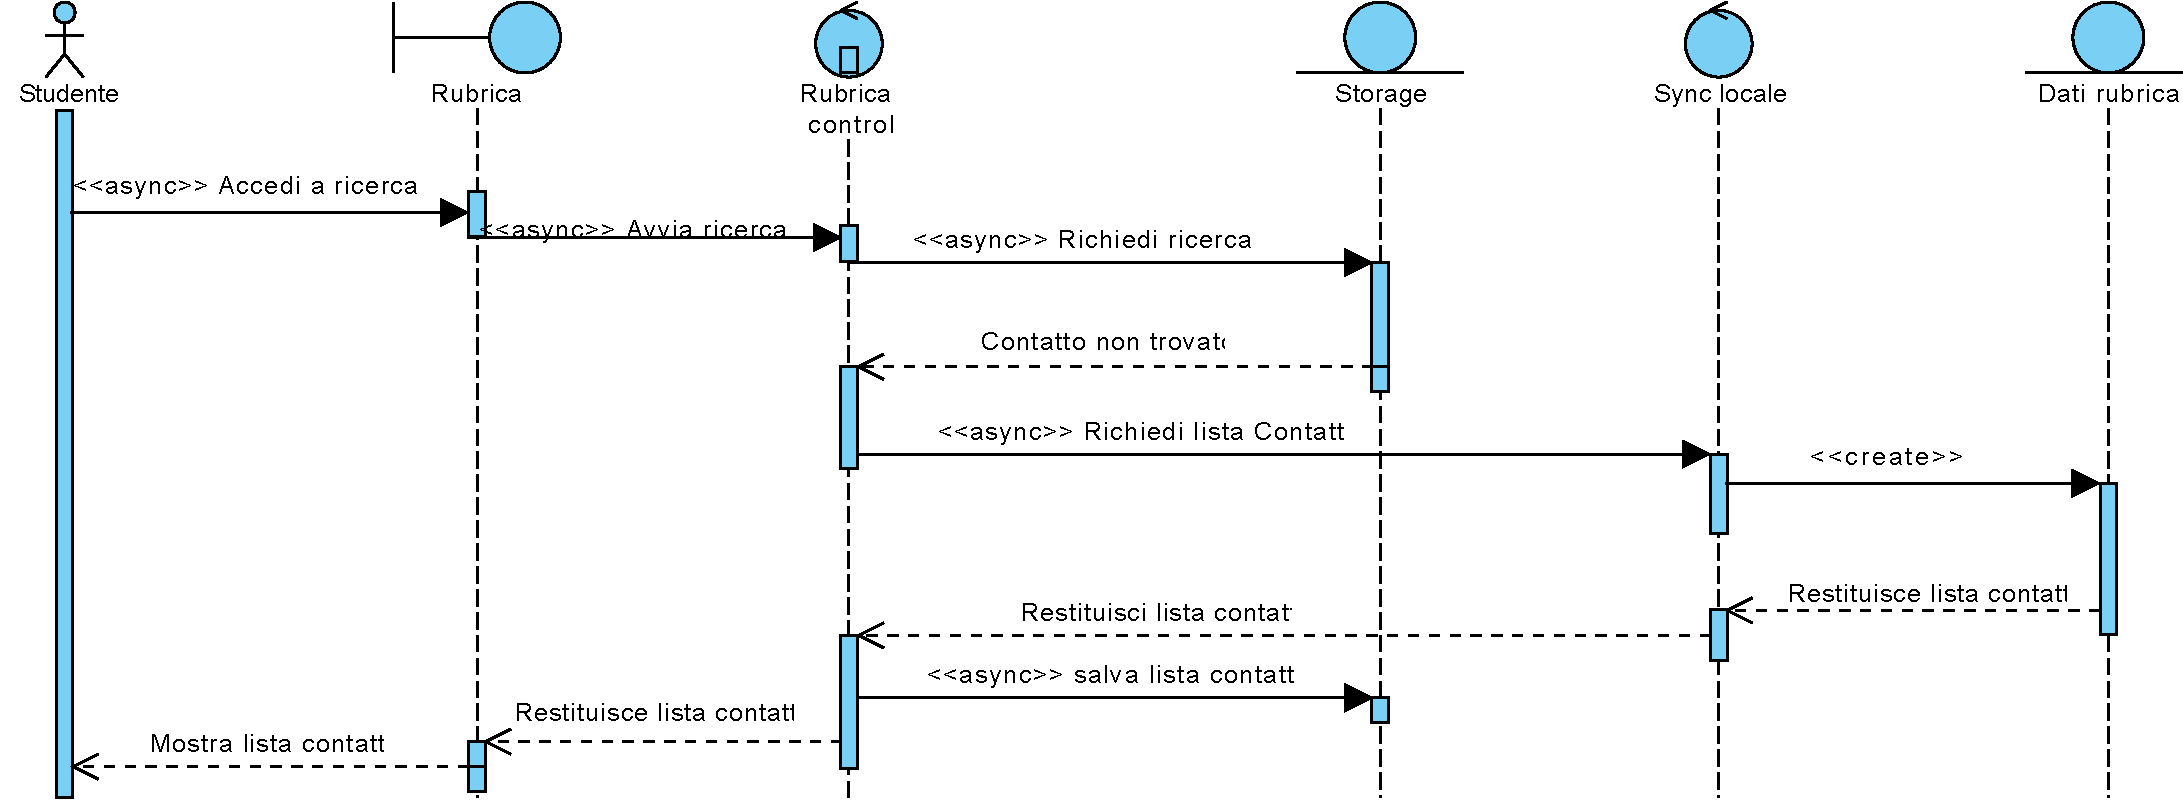
\includegraphics[width=0.9\textwidth]{imgs/gruppo5/sequence1.pdf}
	\caption{Ricerca non filtarta}
	\label{fig:seq1-rubrica}
\end{figure}

\begin{figure}[H]
\centering
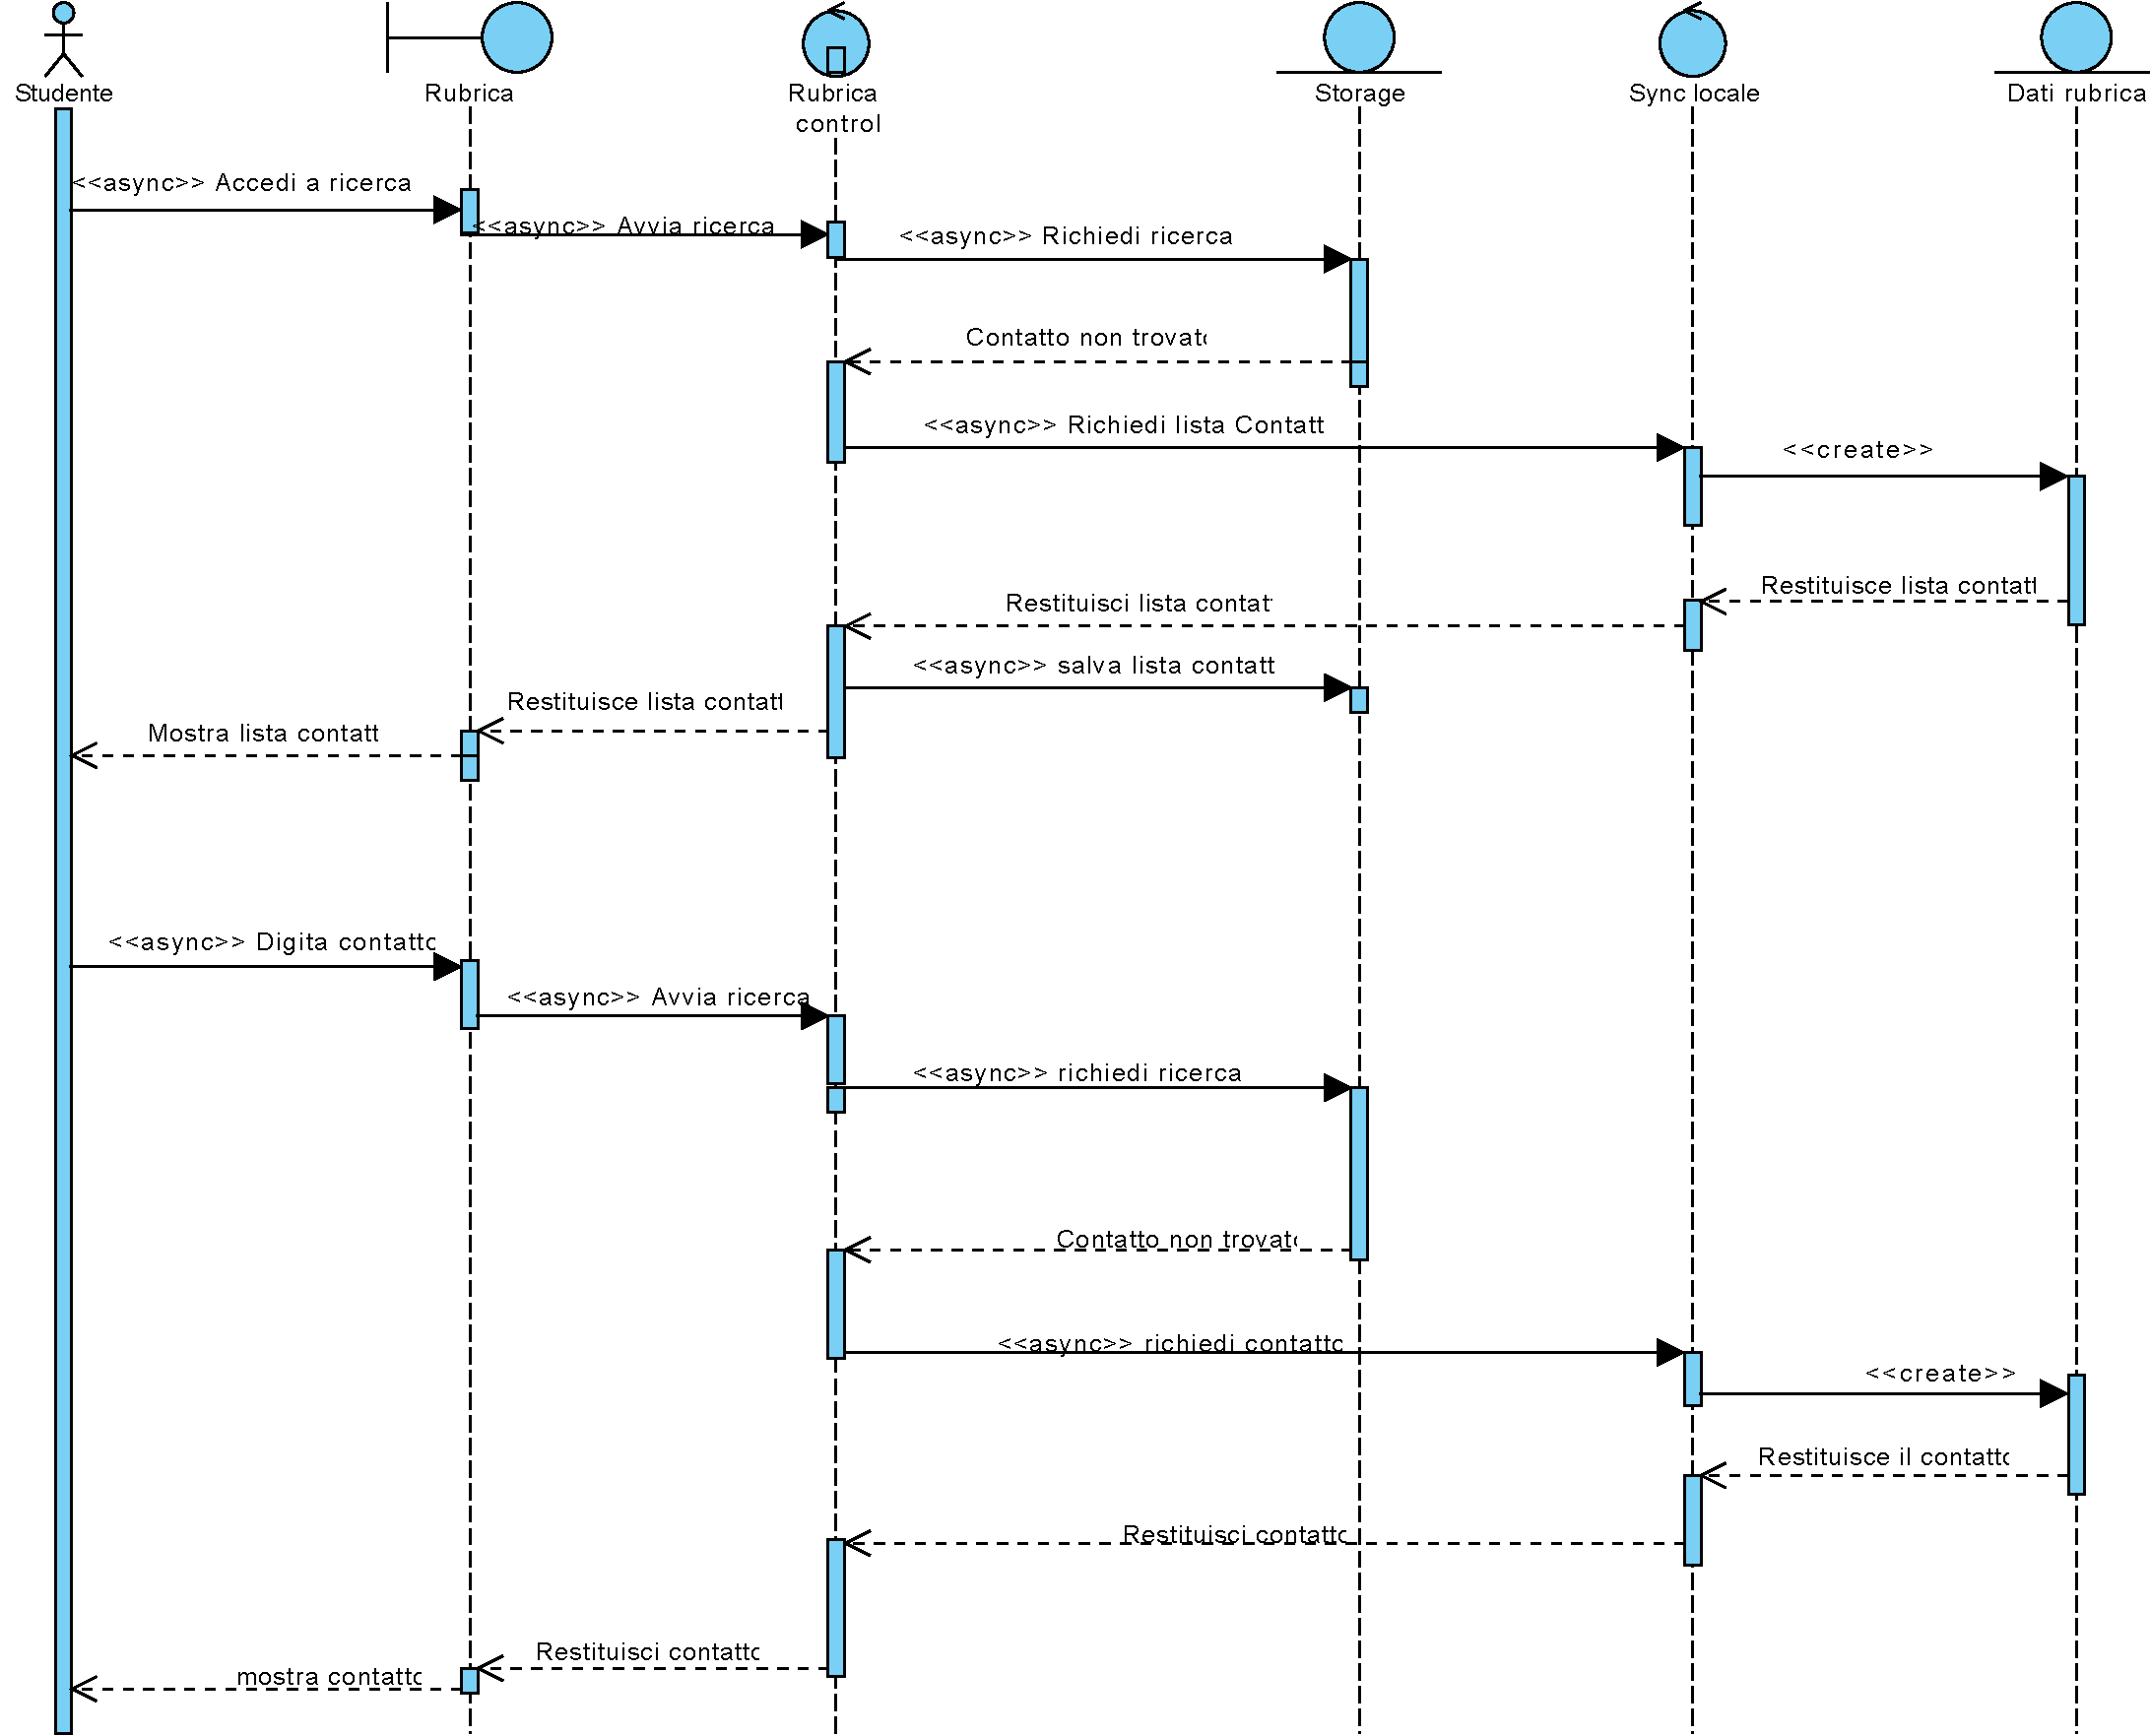
\includegraphics[width=0.9\textwidth]{imgs/gruppo5/sequence2.pdf}
\caption{Ricerca filtarta}
\label{fig:seq2-rubrica}
\end{figure}

\begin{figure}[H]
	\centering
	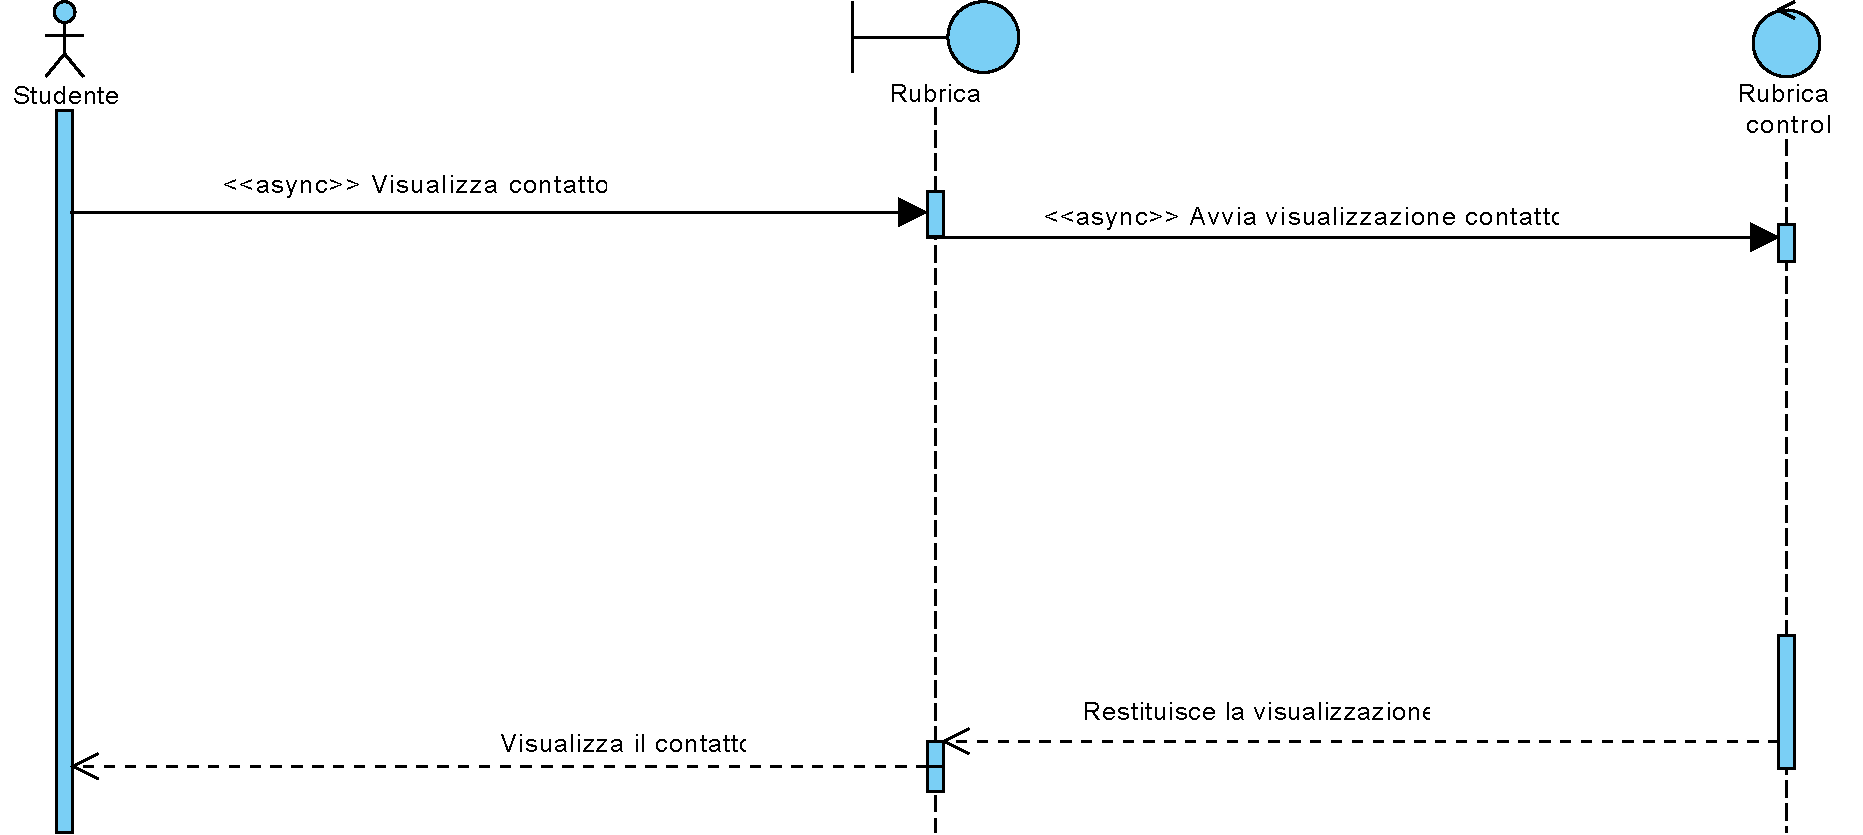
\includegraphics[width=0.9\textwidth]{imgs/gruppo5/sequence3.pdf}
	\caption{Visualizza contatto}
	\label{fig:seq3-rubrica}
\end{figure}

\clearpage
\subsection{Funzionalità previsione media}
\begin{figure}[H]
	\centering
	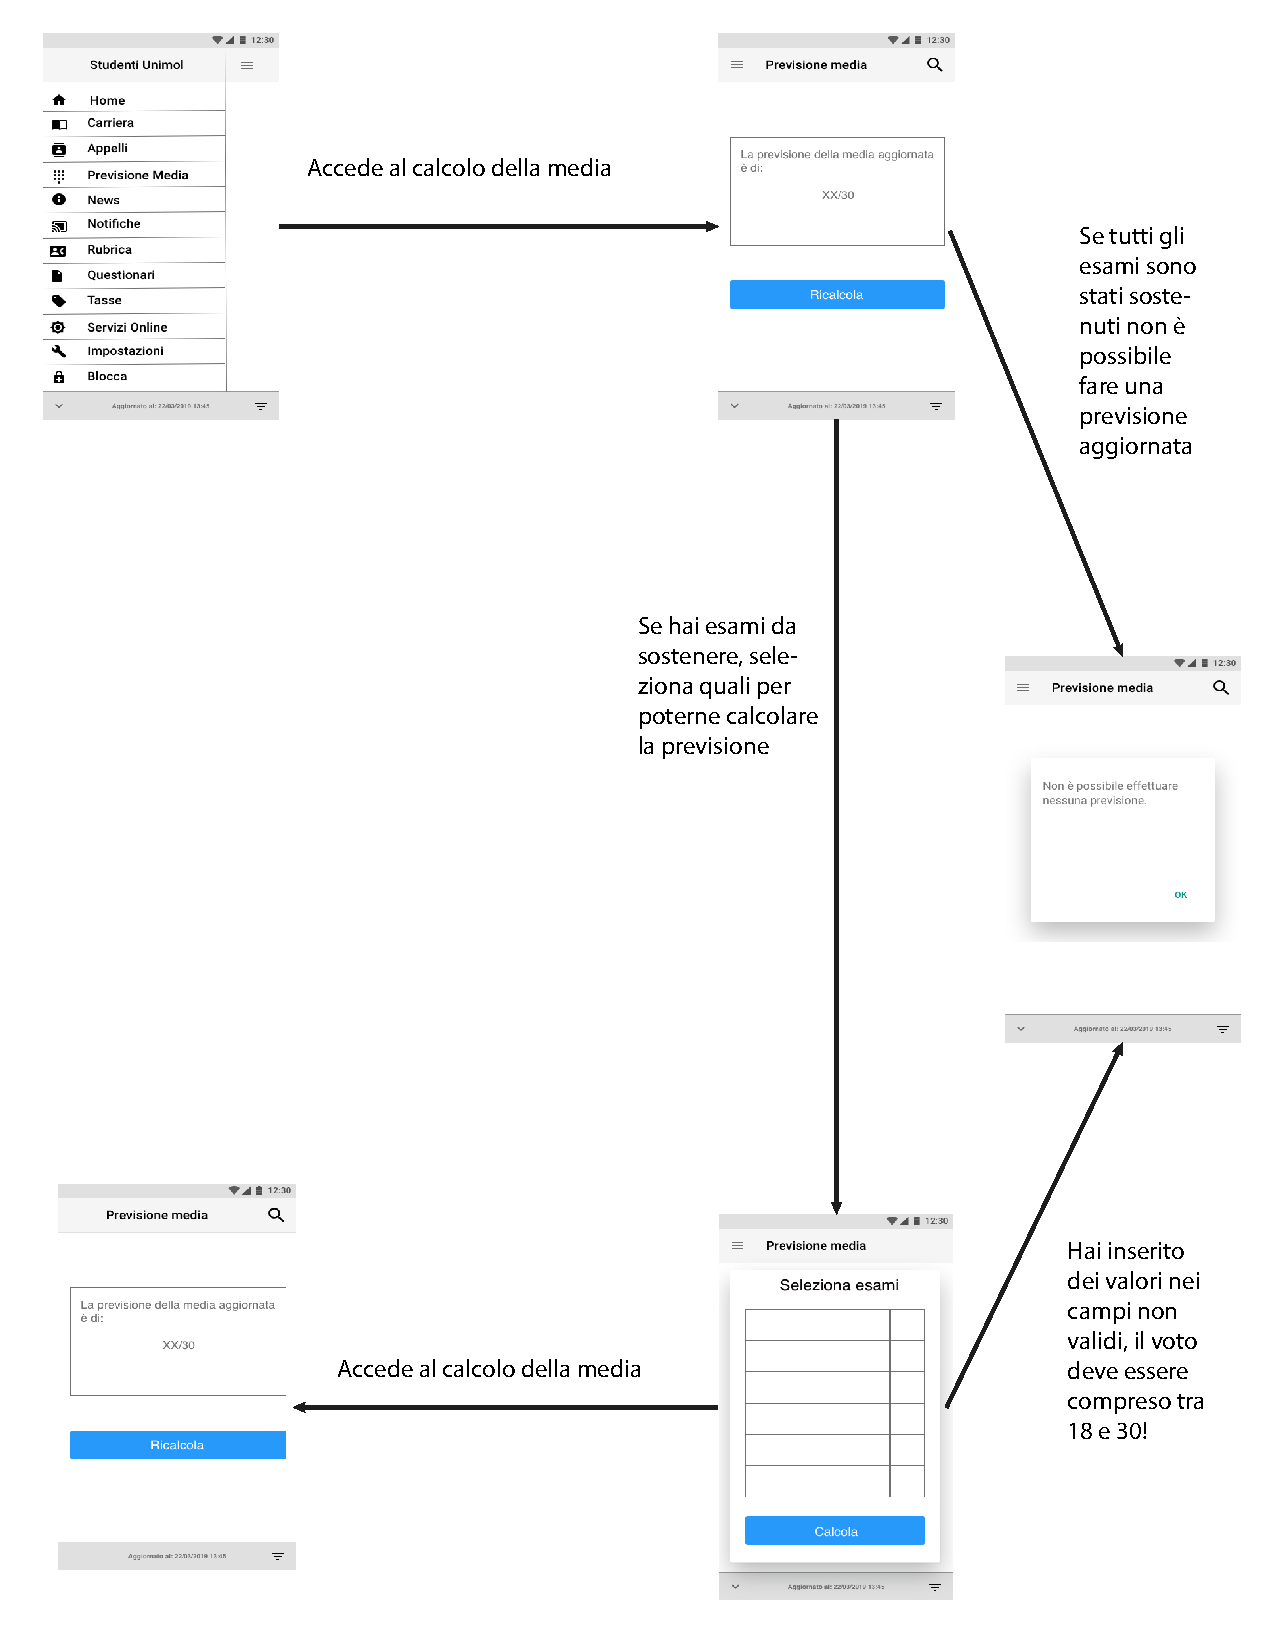
\includegraphics[width=0.9\textwidth]{imgs/gruppo3/media-activity-diagram.pdf}
	\caption{Diagramma di attività}
	\label{fig:act-rubrica}
\end{figure}

\clearpage
\section{Diagrammi dei casi d'uso}

\subsection{Funzionalità Gestione Piano di Studio}
\begin{figure} [h]
	\centering
	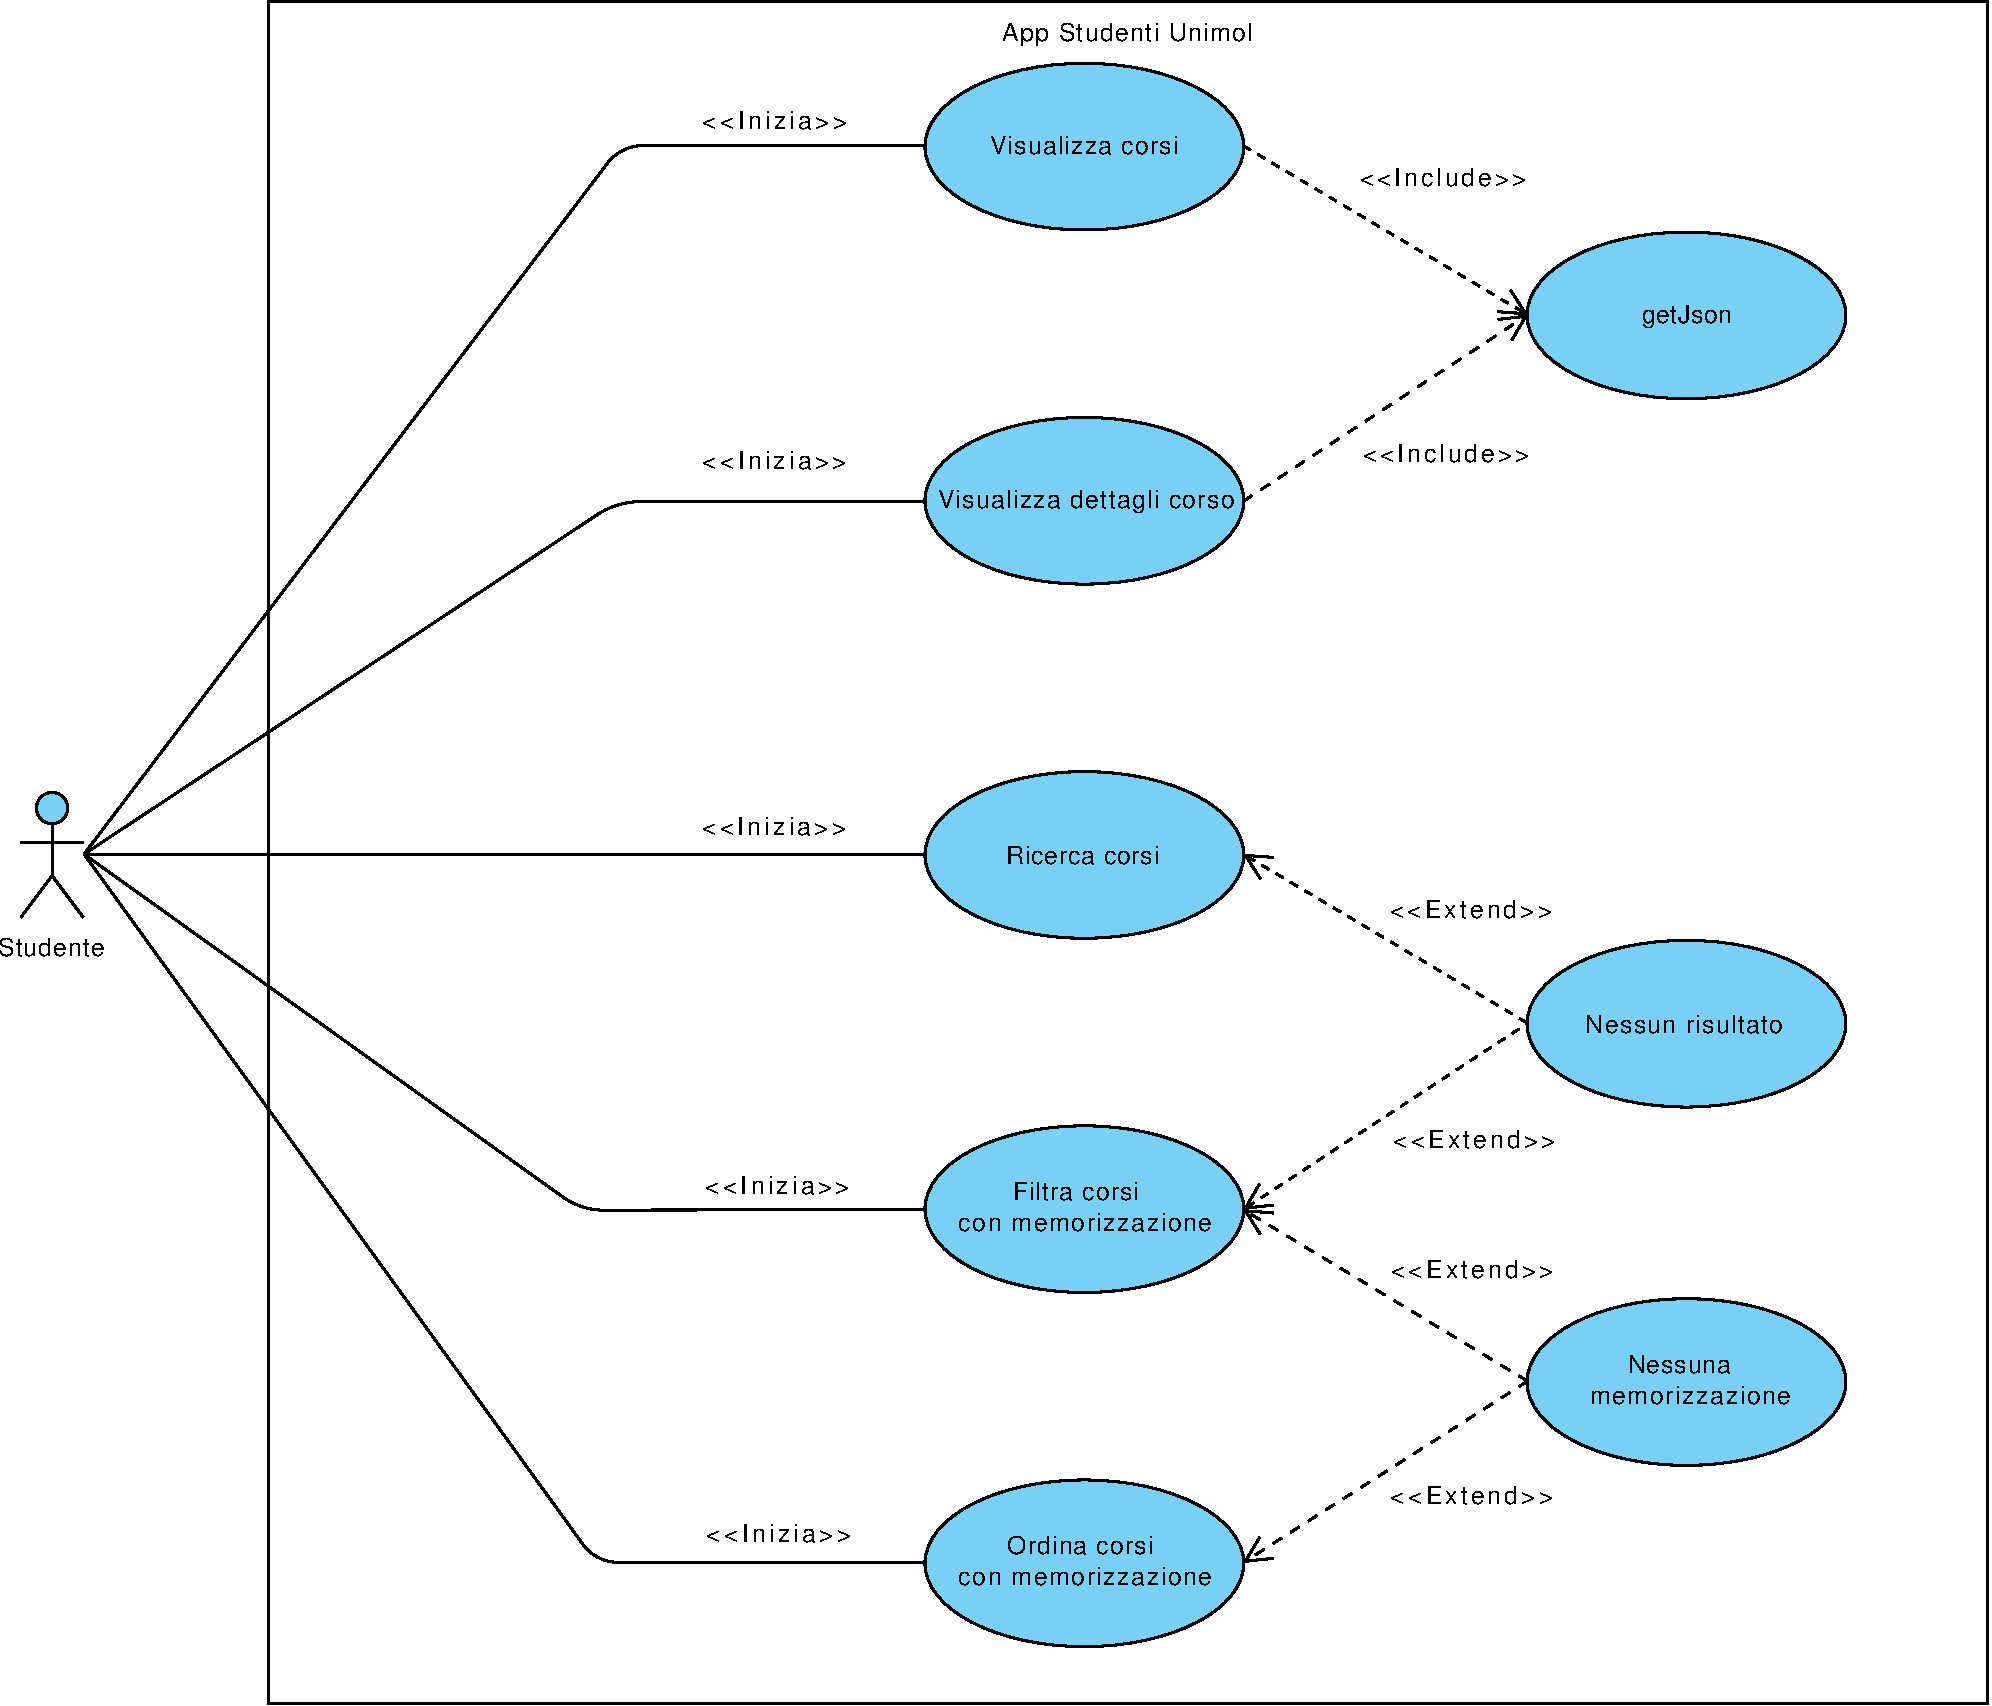
\includegraphics[width=6.5in]{imgs/gruppo1/use_case_diagrams/UCD1-gestione_piano_di_studio.pdf}
	\caption{Diagramma caso d'uso- Gestione piano di studio}
	\label{diag:gestionePianoStudio}
\end{figure}
\clearpage
\subsection{Funzionalità Gestione appelli}
\clearpage
%\paragraph{Visualizza appelli disponibil}
\begin{figure}
	\centering
	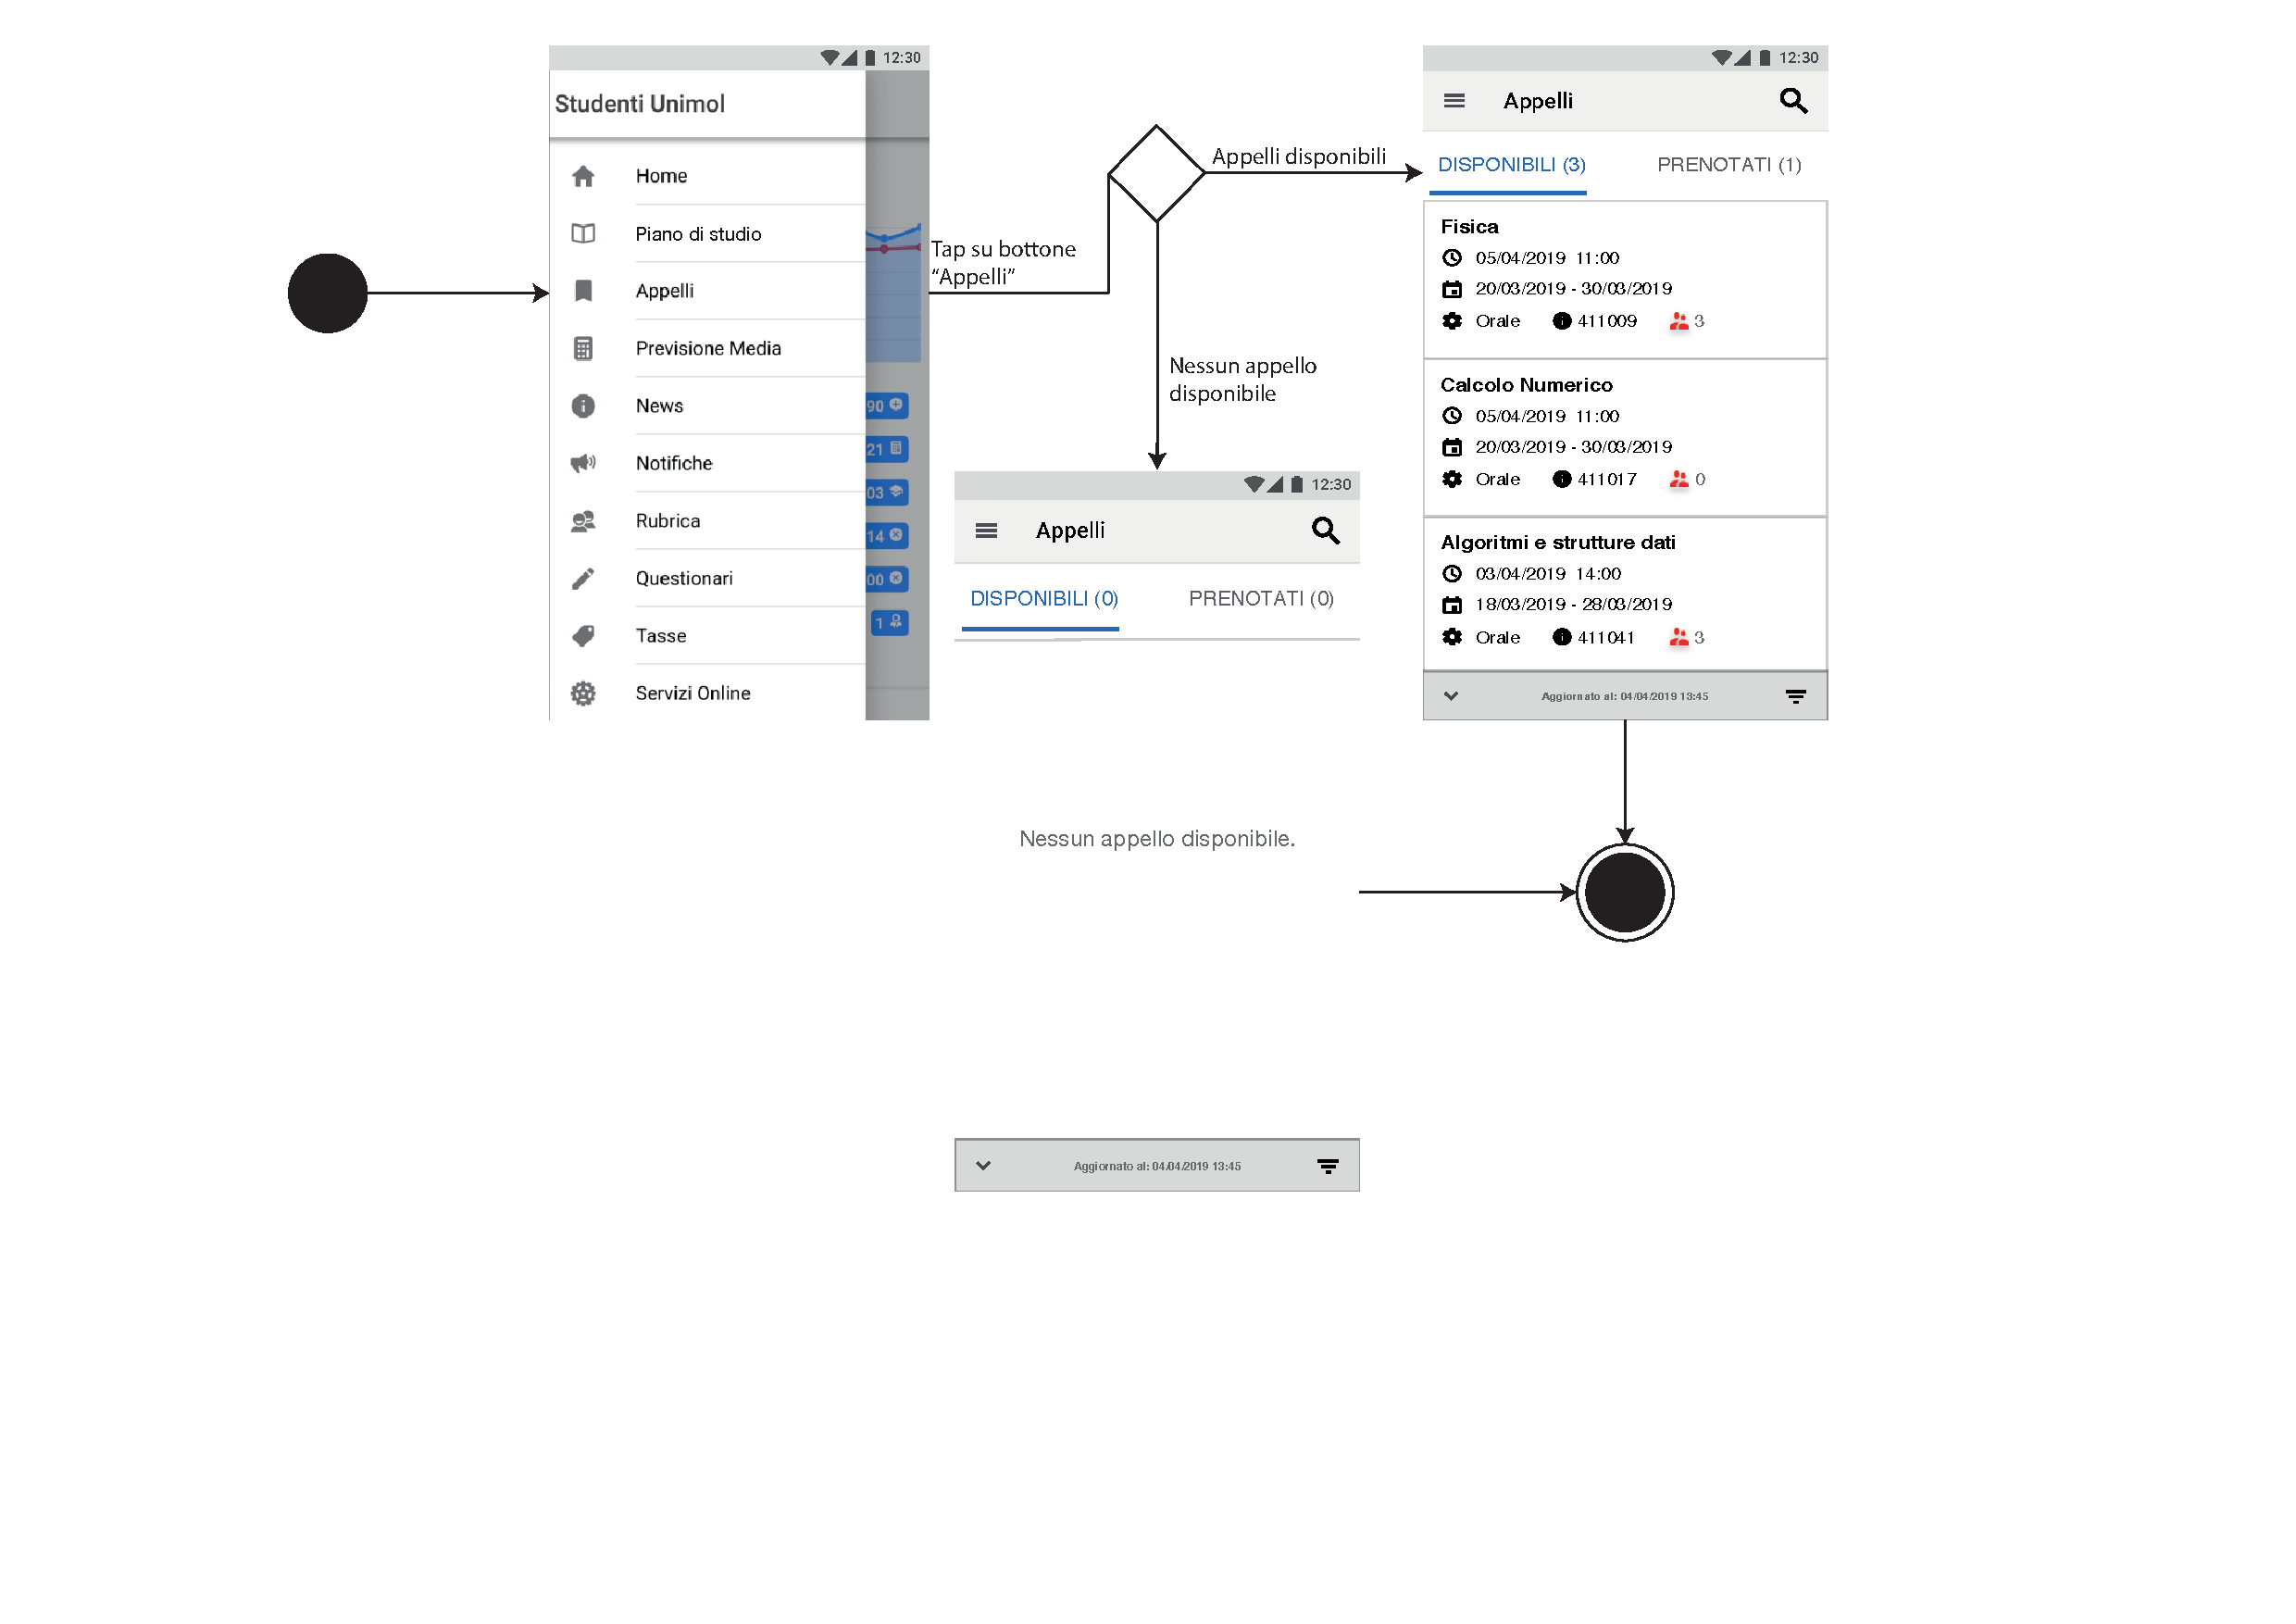
\includegraphics[width=6in]{imgs/gruppo1/activity_diagrams/AD6_visualizza_appelli_disponibili.pdf}
	\caption{Activity Diagram - Visualizza appelli disponibili}
	\label{diag:visualizzaAppelliDisponibiliAD}
\end{figure}
\newpage

%\paragraph{Visualizza appelli prenotati}
\begin{figure}
	\centering
	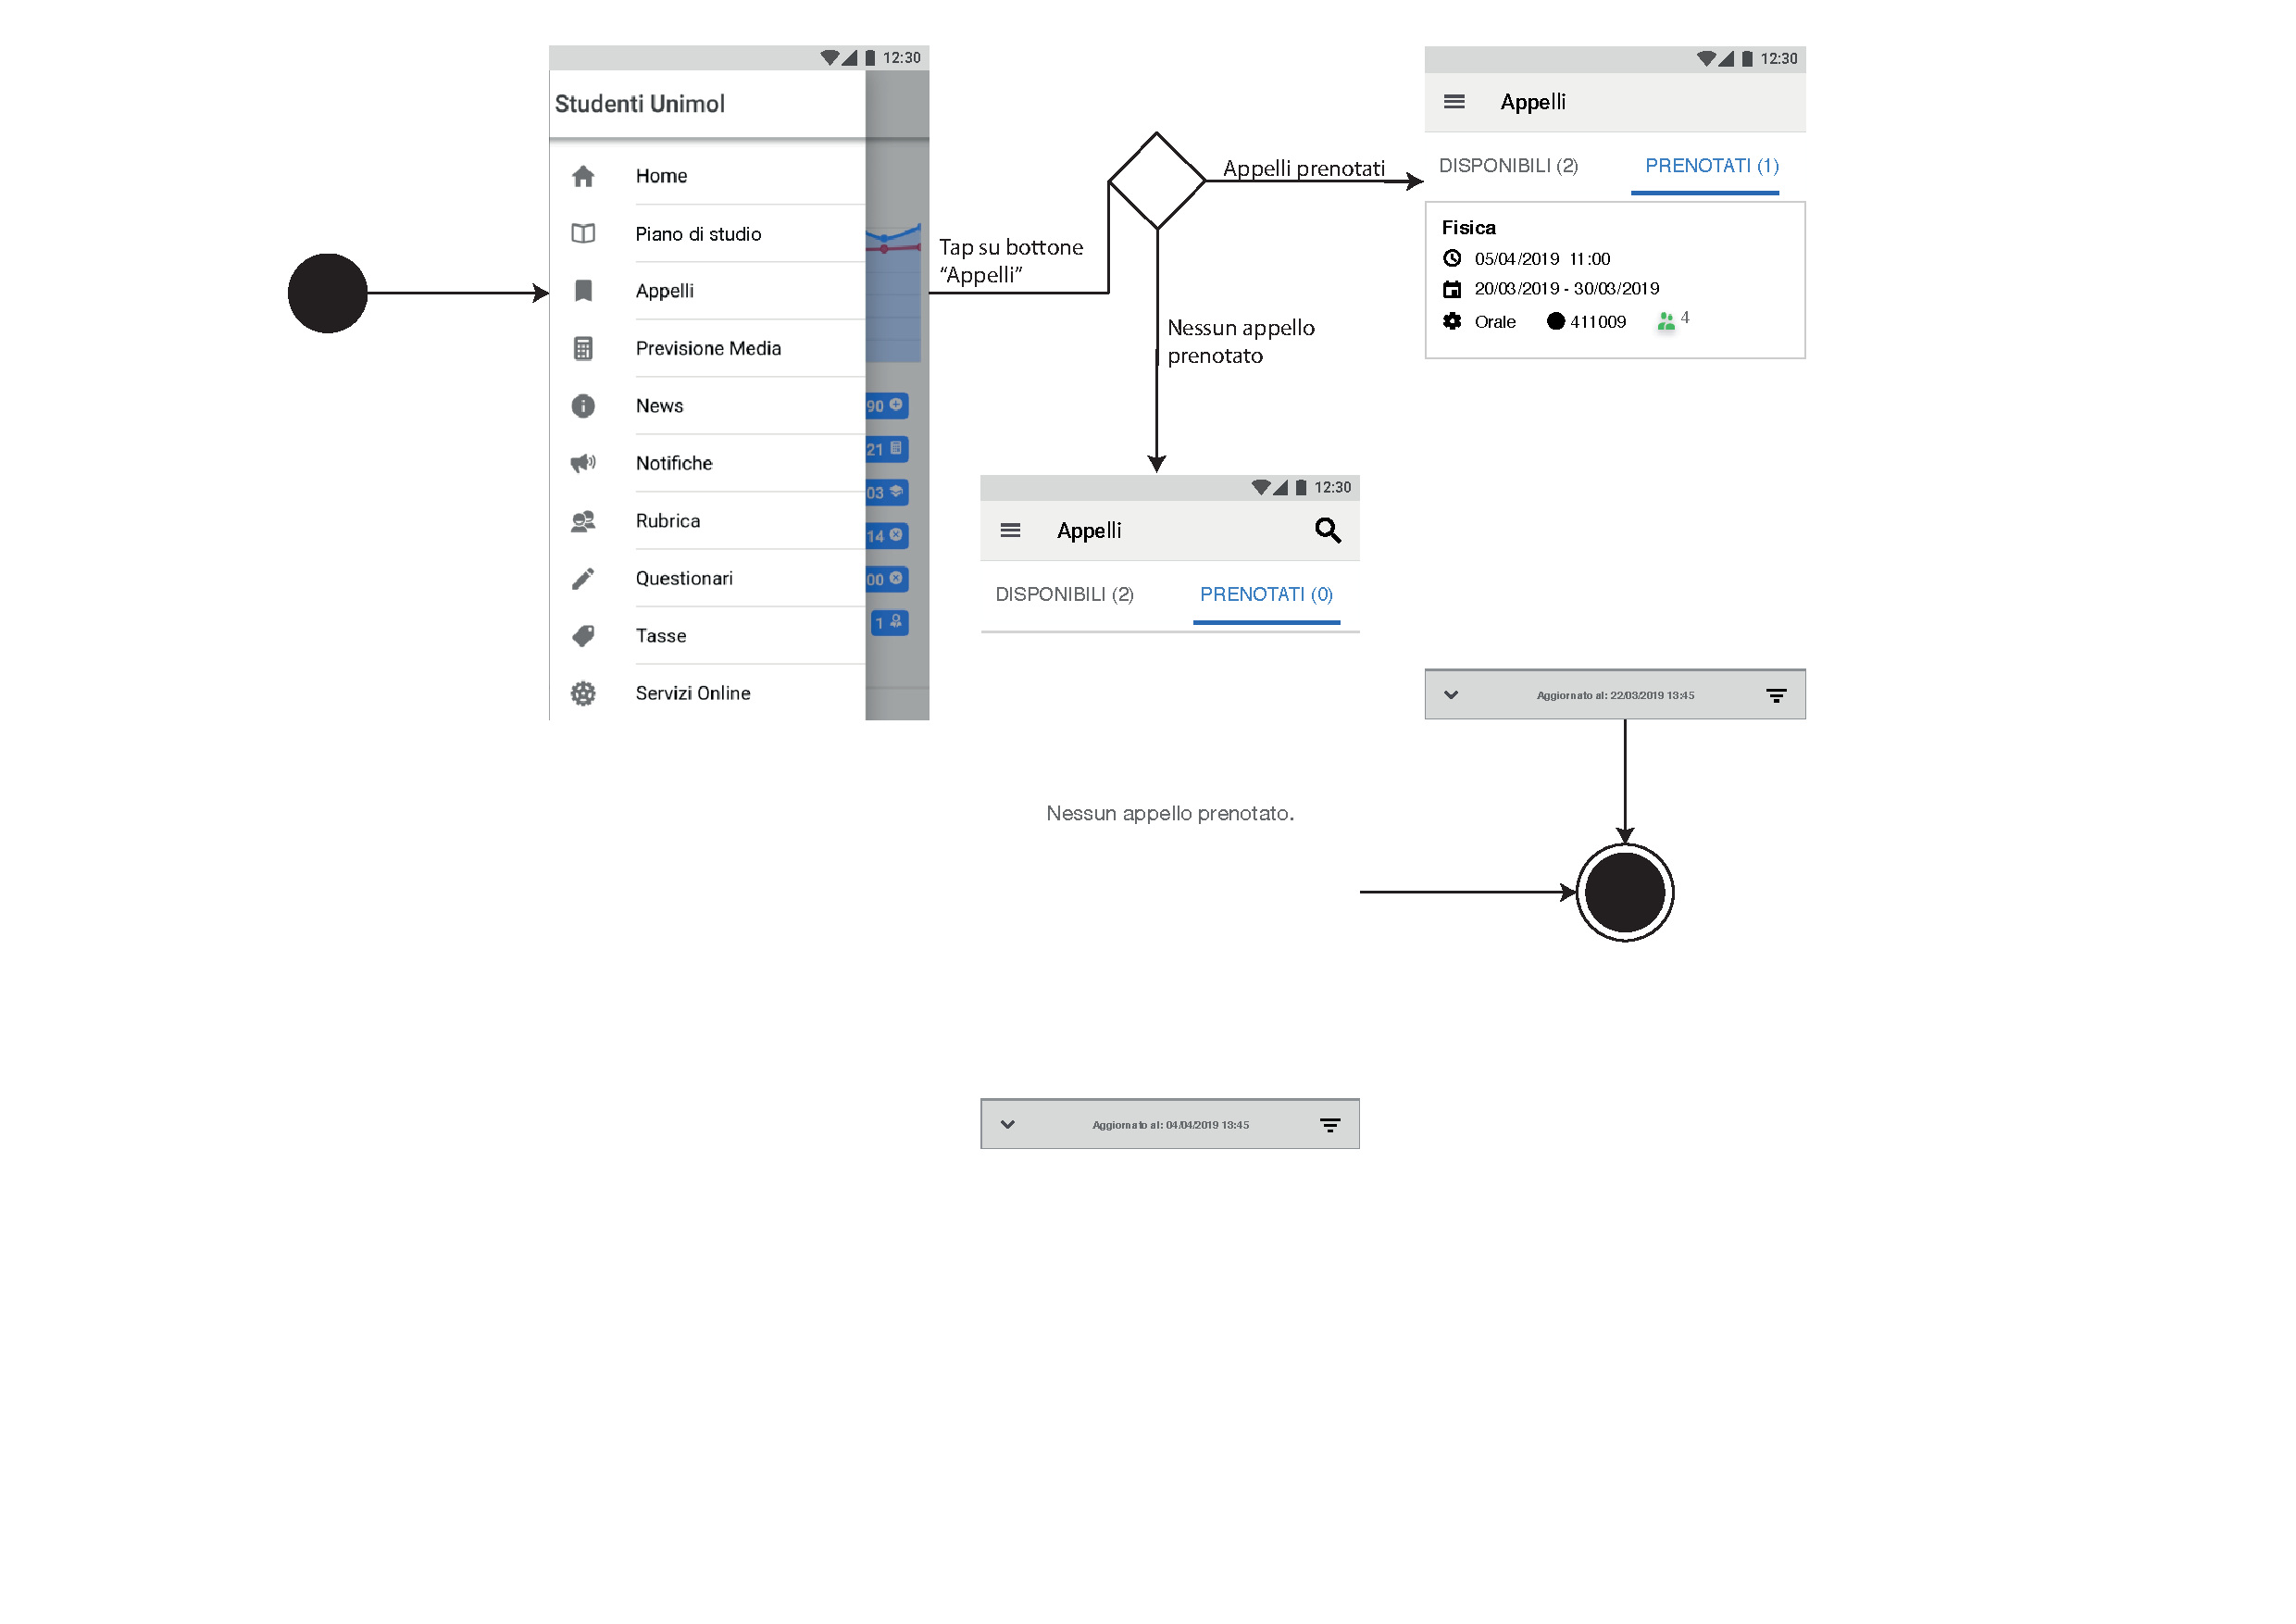
\includegraphics[width=6in]{imgs/gruppo1/activity_diagrams/AD7_visualizza_appelli_prenotati.pdf}
	\caption{Activity Diagram - Visualizza appelli prenotati}
	\label{diag:visualizzaAppelliPrenotatiAD}
\end{figure}
\newpage

%\paragraph{Ricerca appelli disponibili}
\begin{figure}
	\centering
	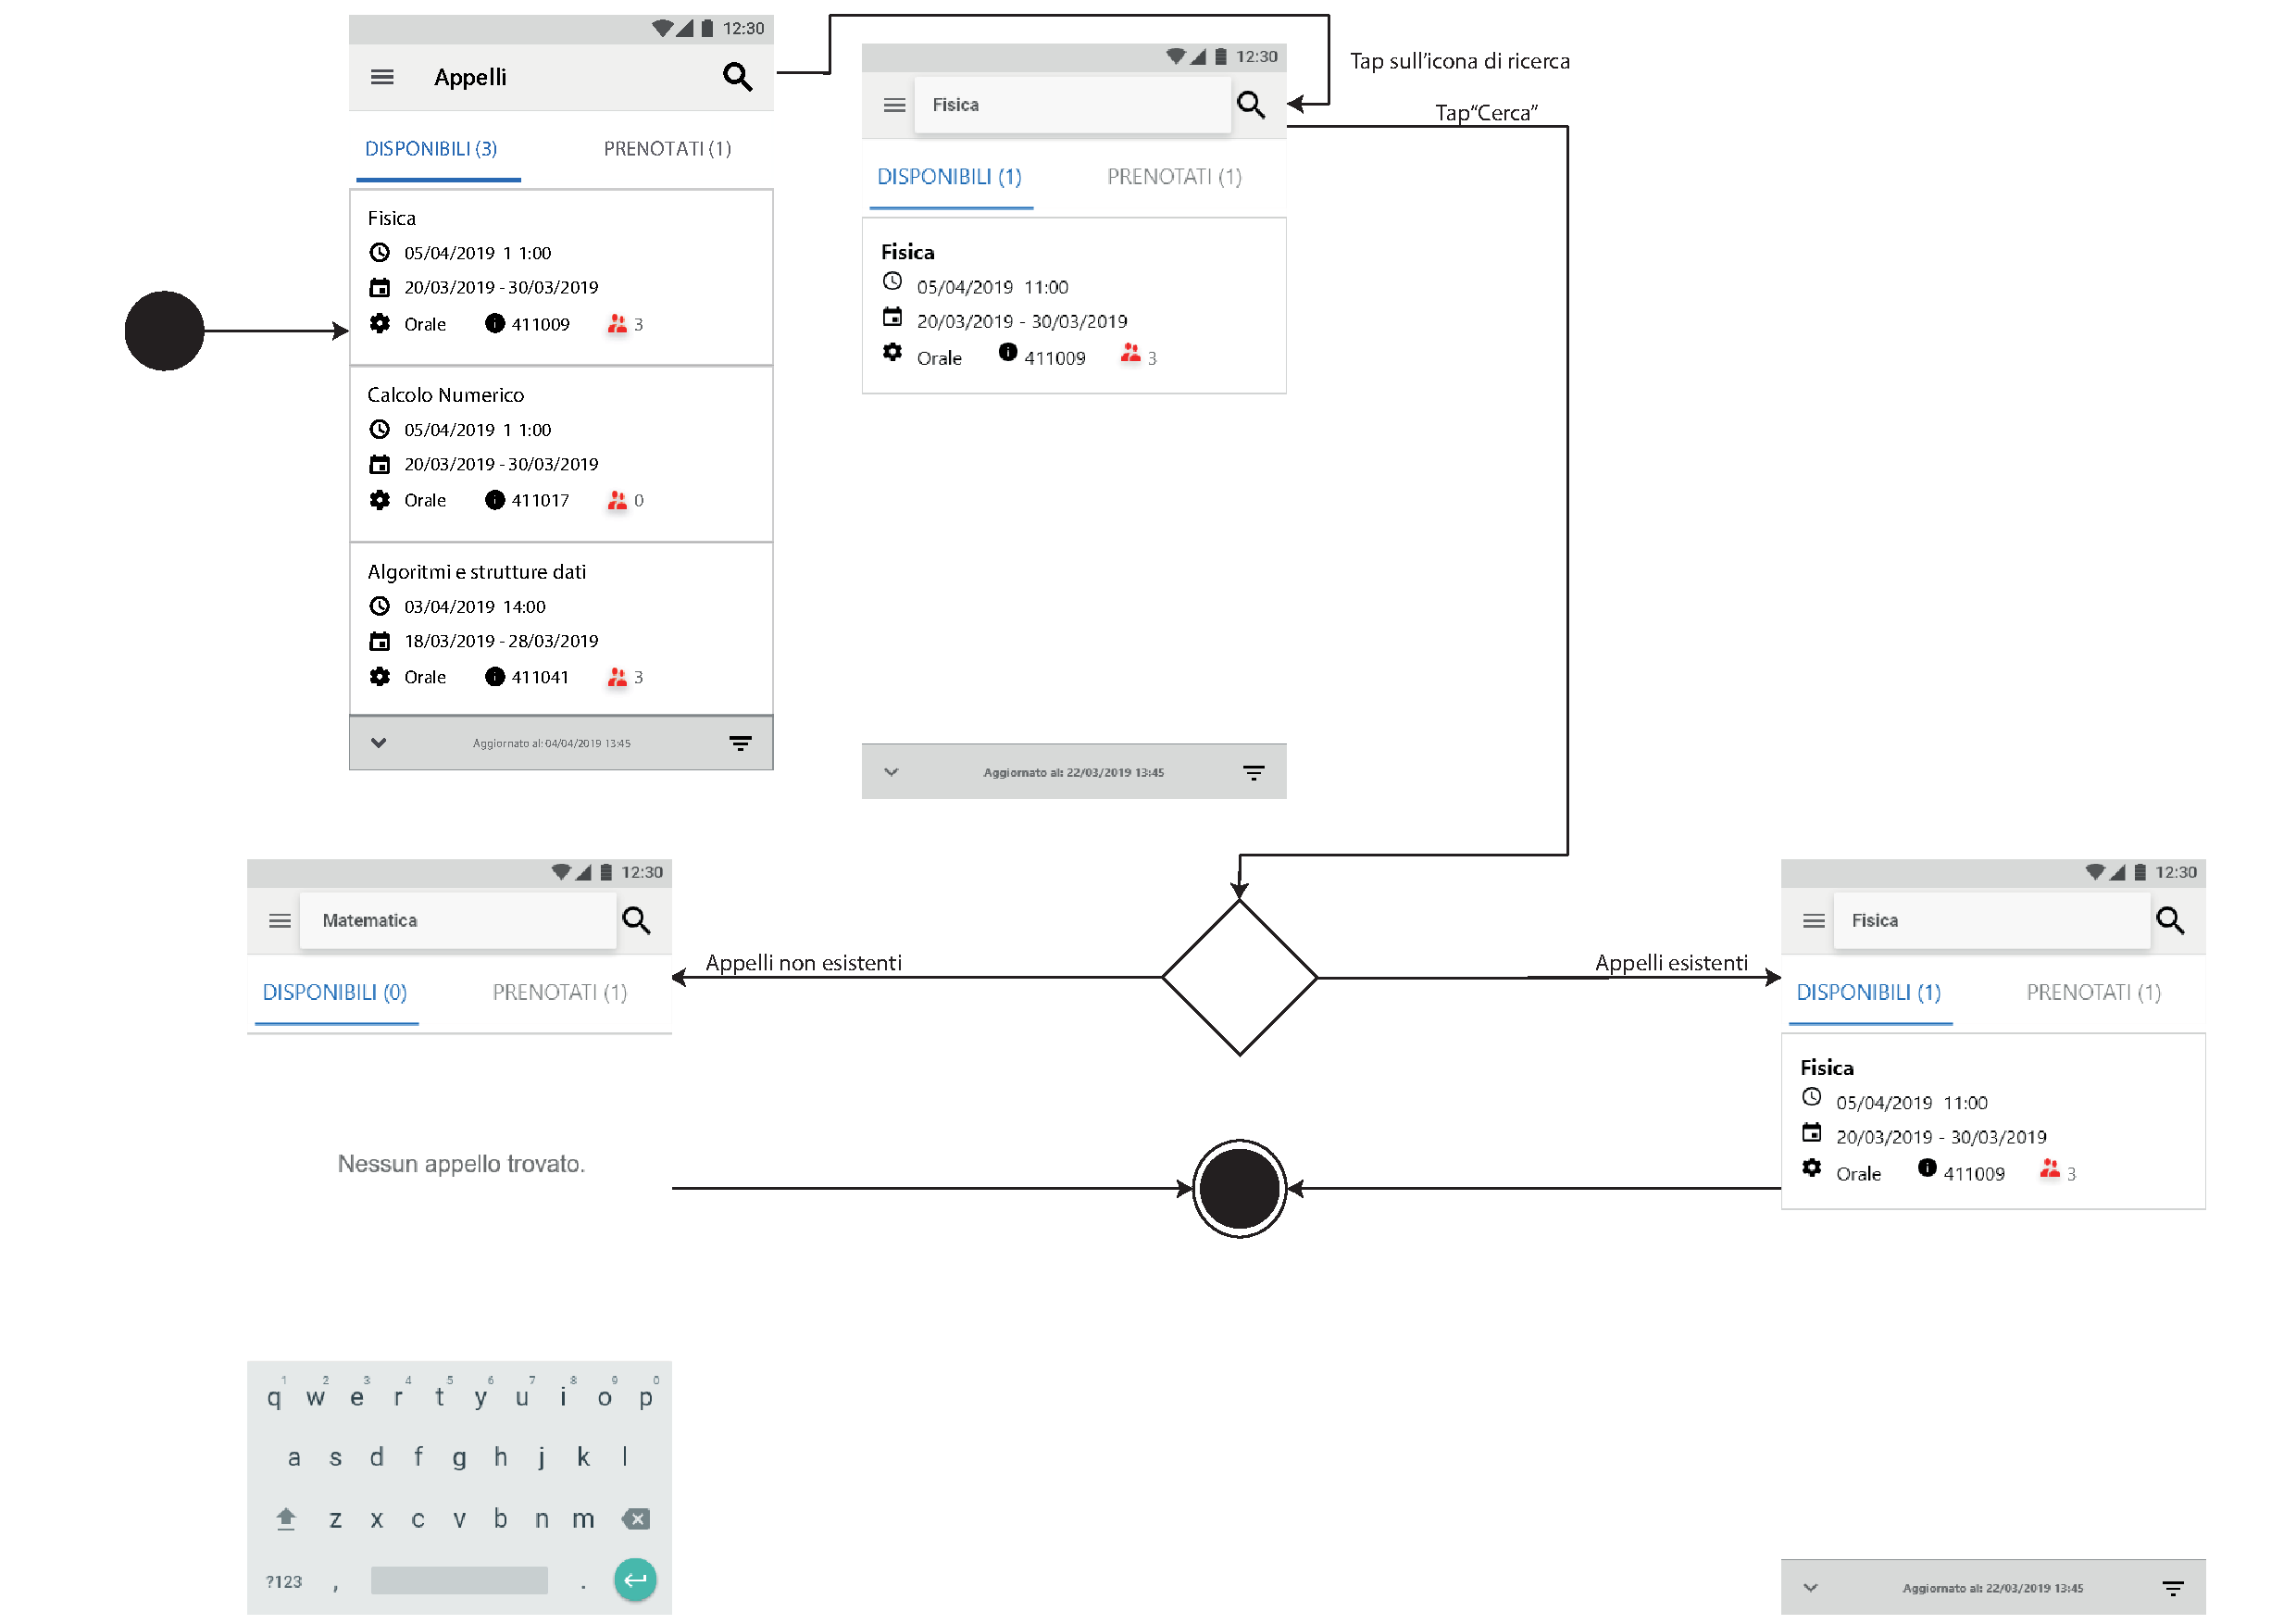
\includegraphics[width=6in]{imgs/gruppo1/activity_diagrams/AD8_Ricerca_appelli.pdf}
	\caption{Activity Diagram - Ricerca appelli disponibili}
	\label{diag:ricercaAppelliDisponibiliAD}
\end{figure}
\newpage

%\paragraph{Filtra appelli disponibili con memorizzazione }
\begin{figure}
	\centering
	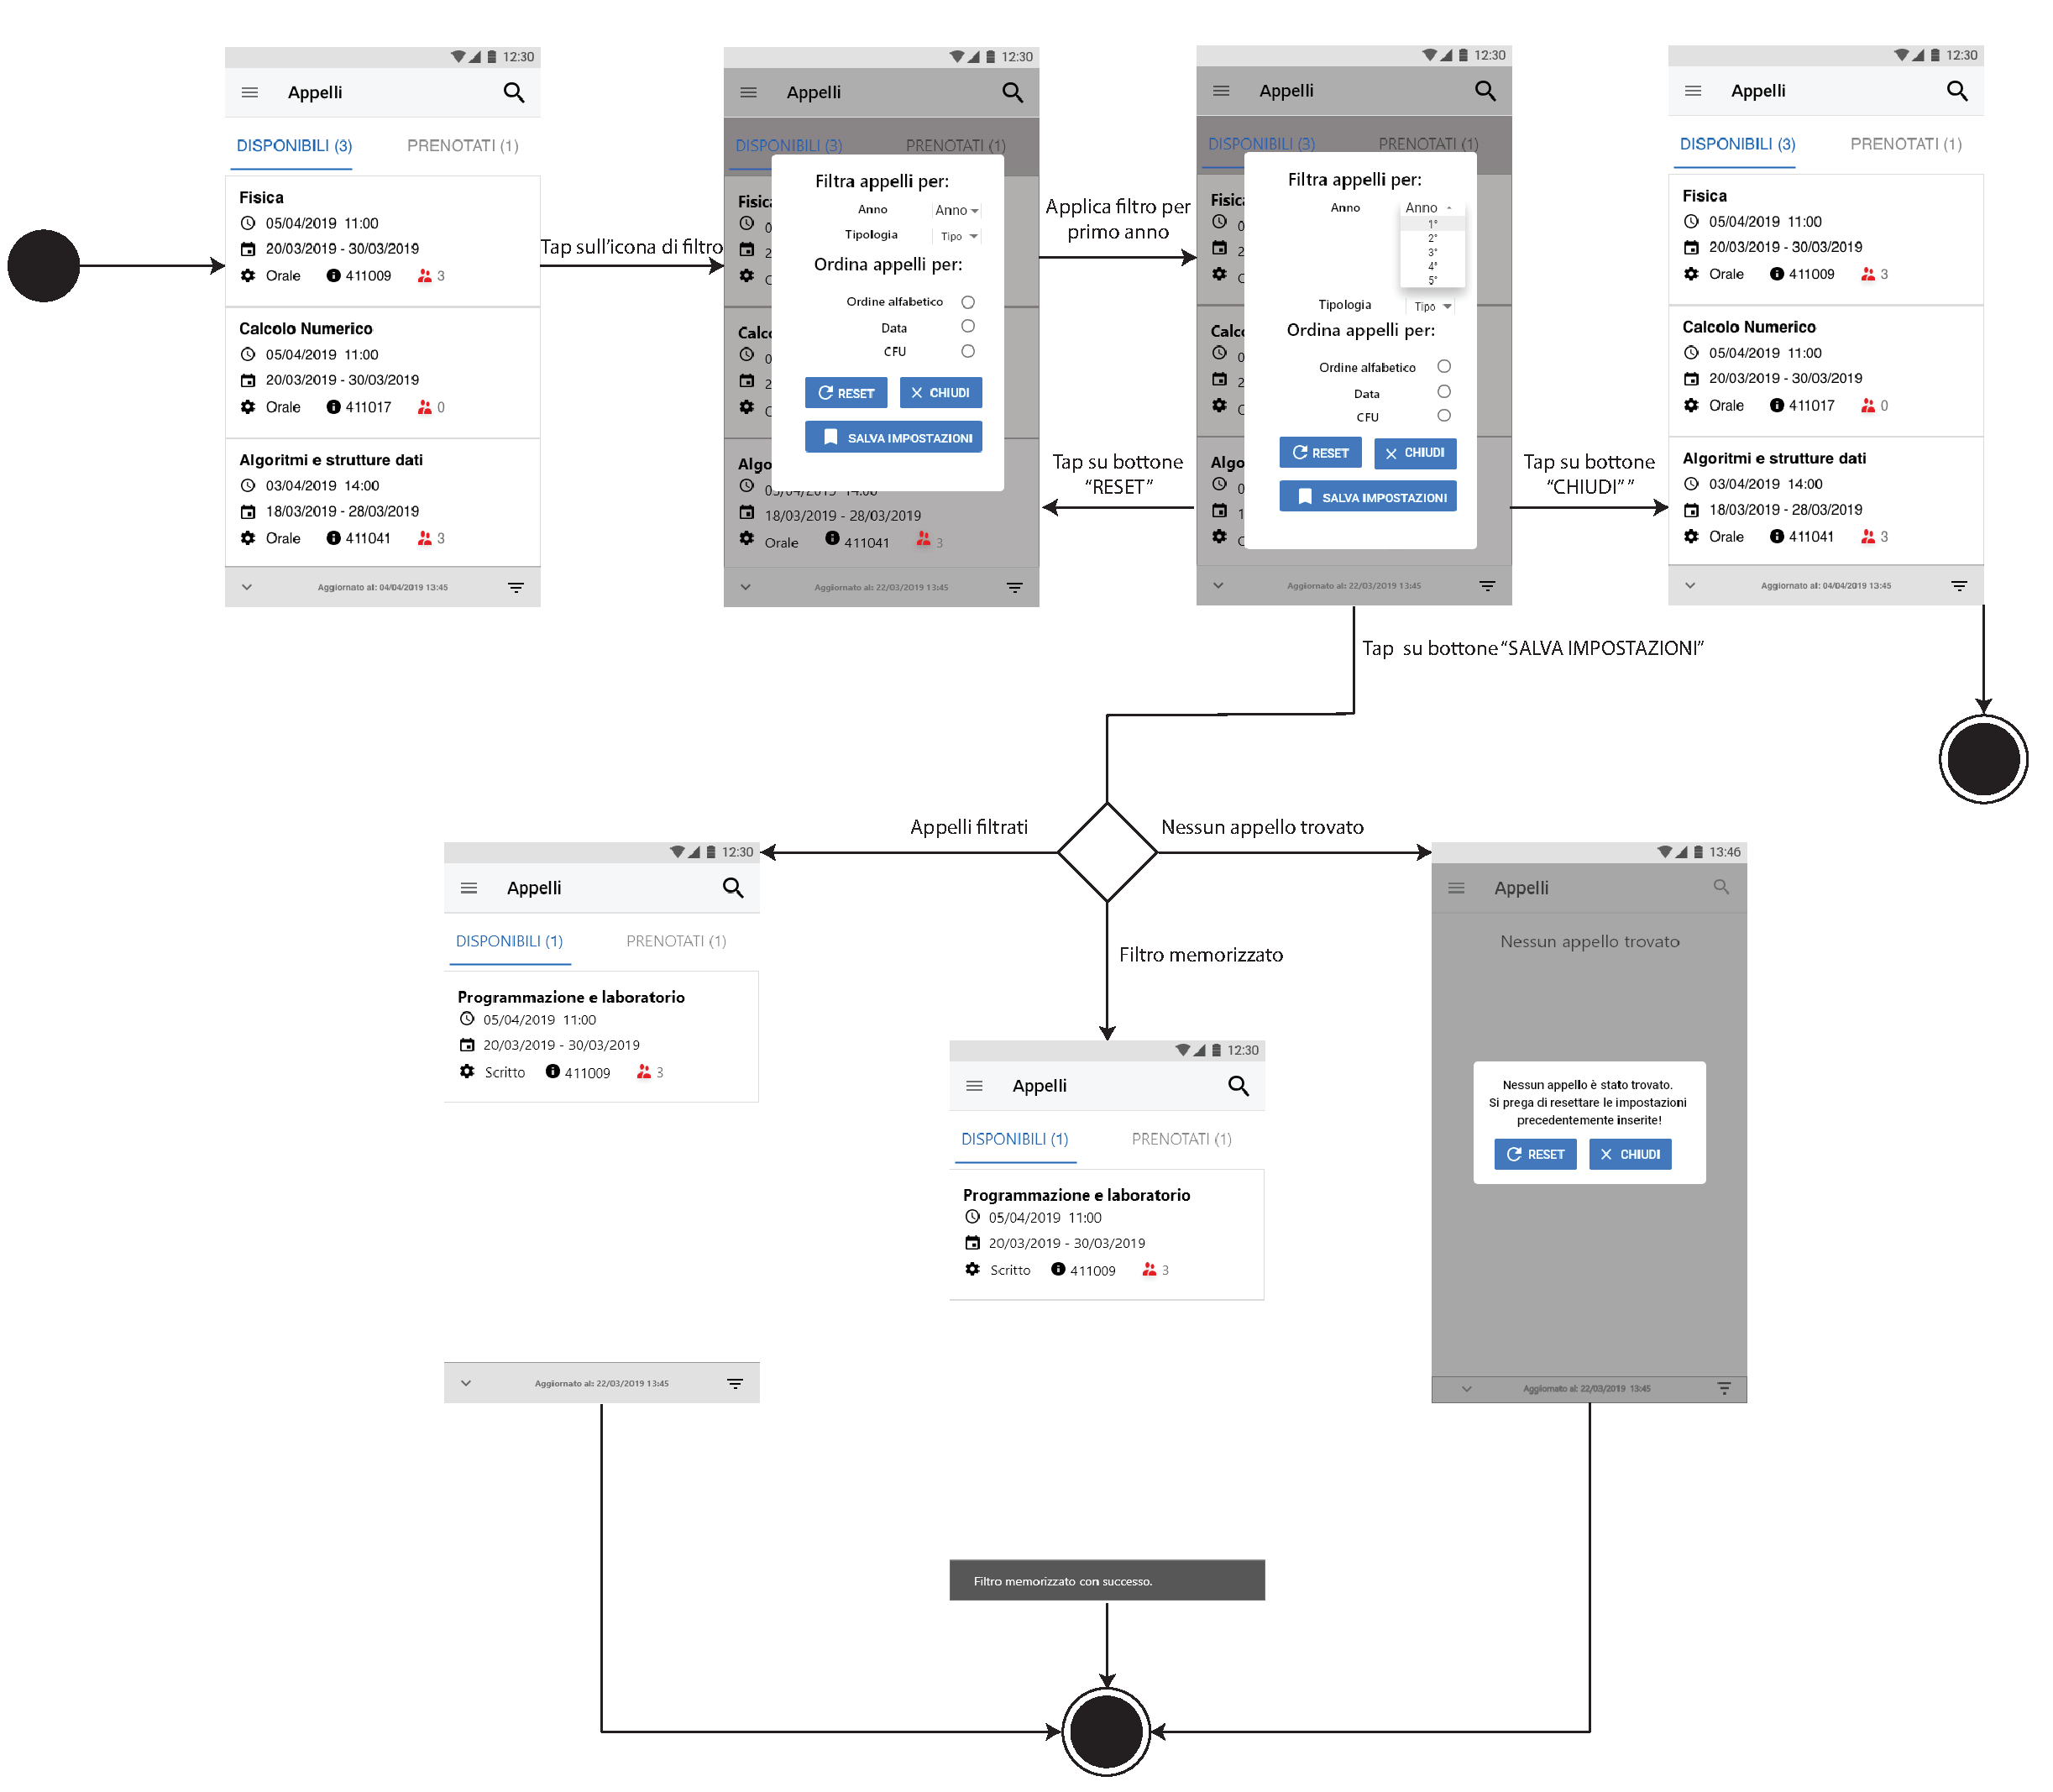
\includegraphics[width=6in]{imgs/gruppo1/activity_diagrams/AD9_filtrati_appelli.pdf}
	\caption{Activity Diagram - Filtra appelli disponibili con memorizzazione}
	\label{diag:filtraAppelliDisponibiliConMemAD}
\end{figure}
\newpage

%\paragraph{Ordina appelli disponibili con memorizzazione }
\begin{figure}
	\centering
	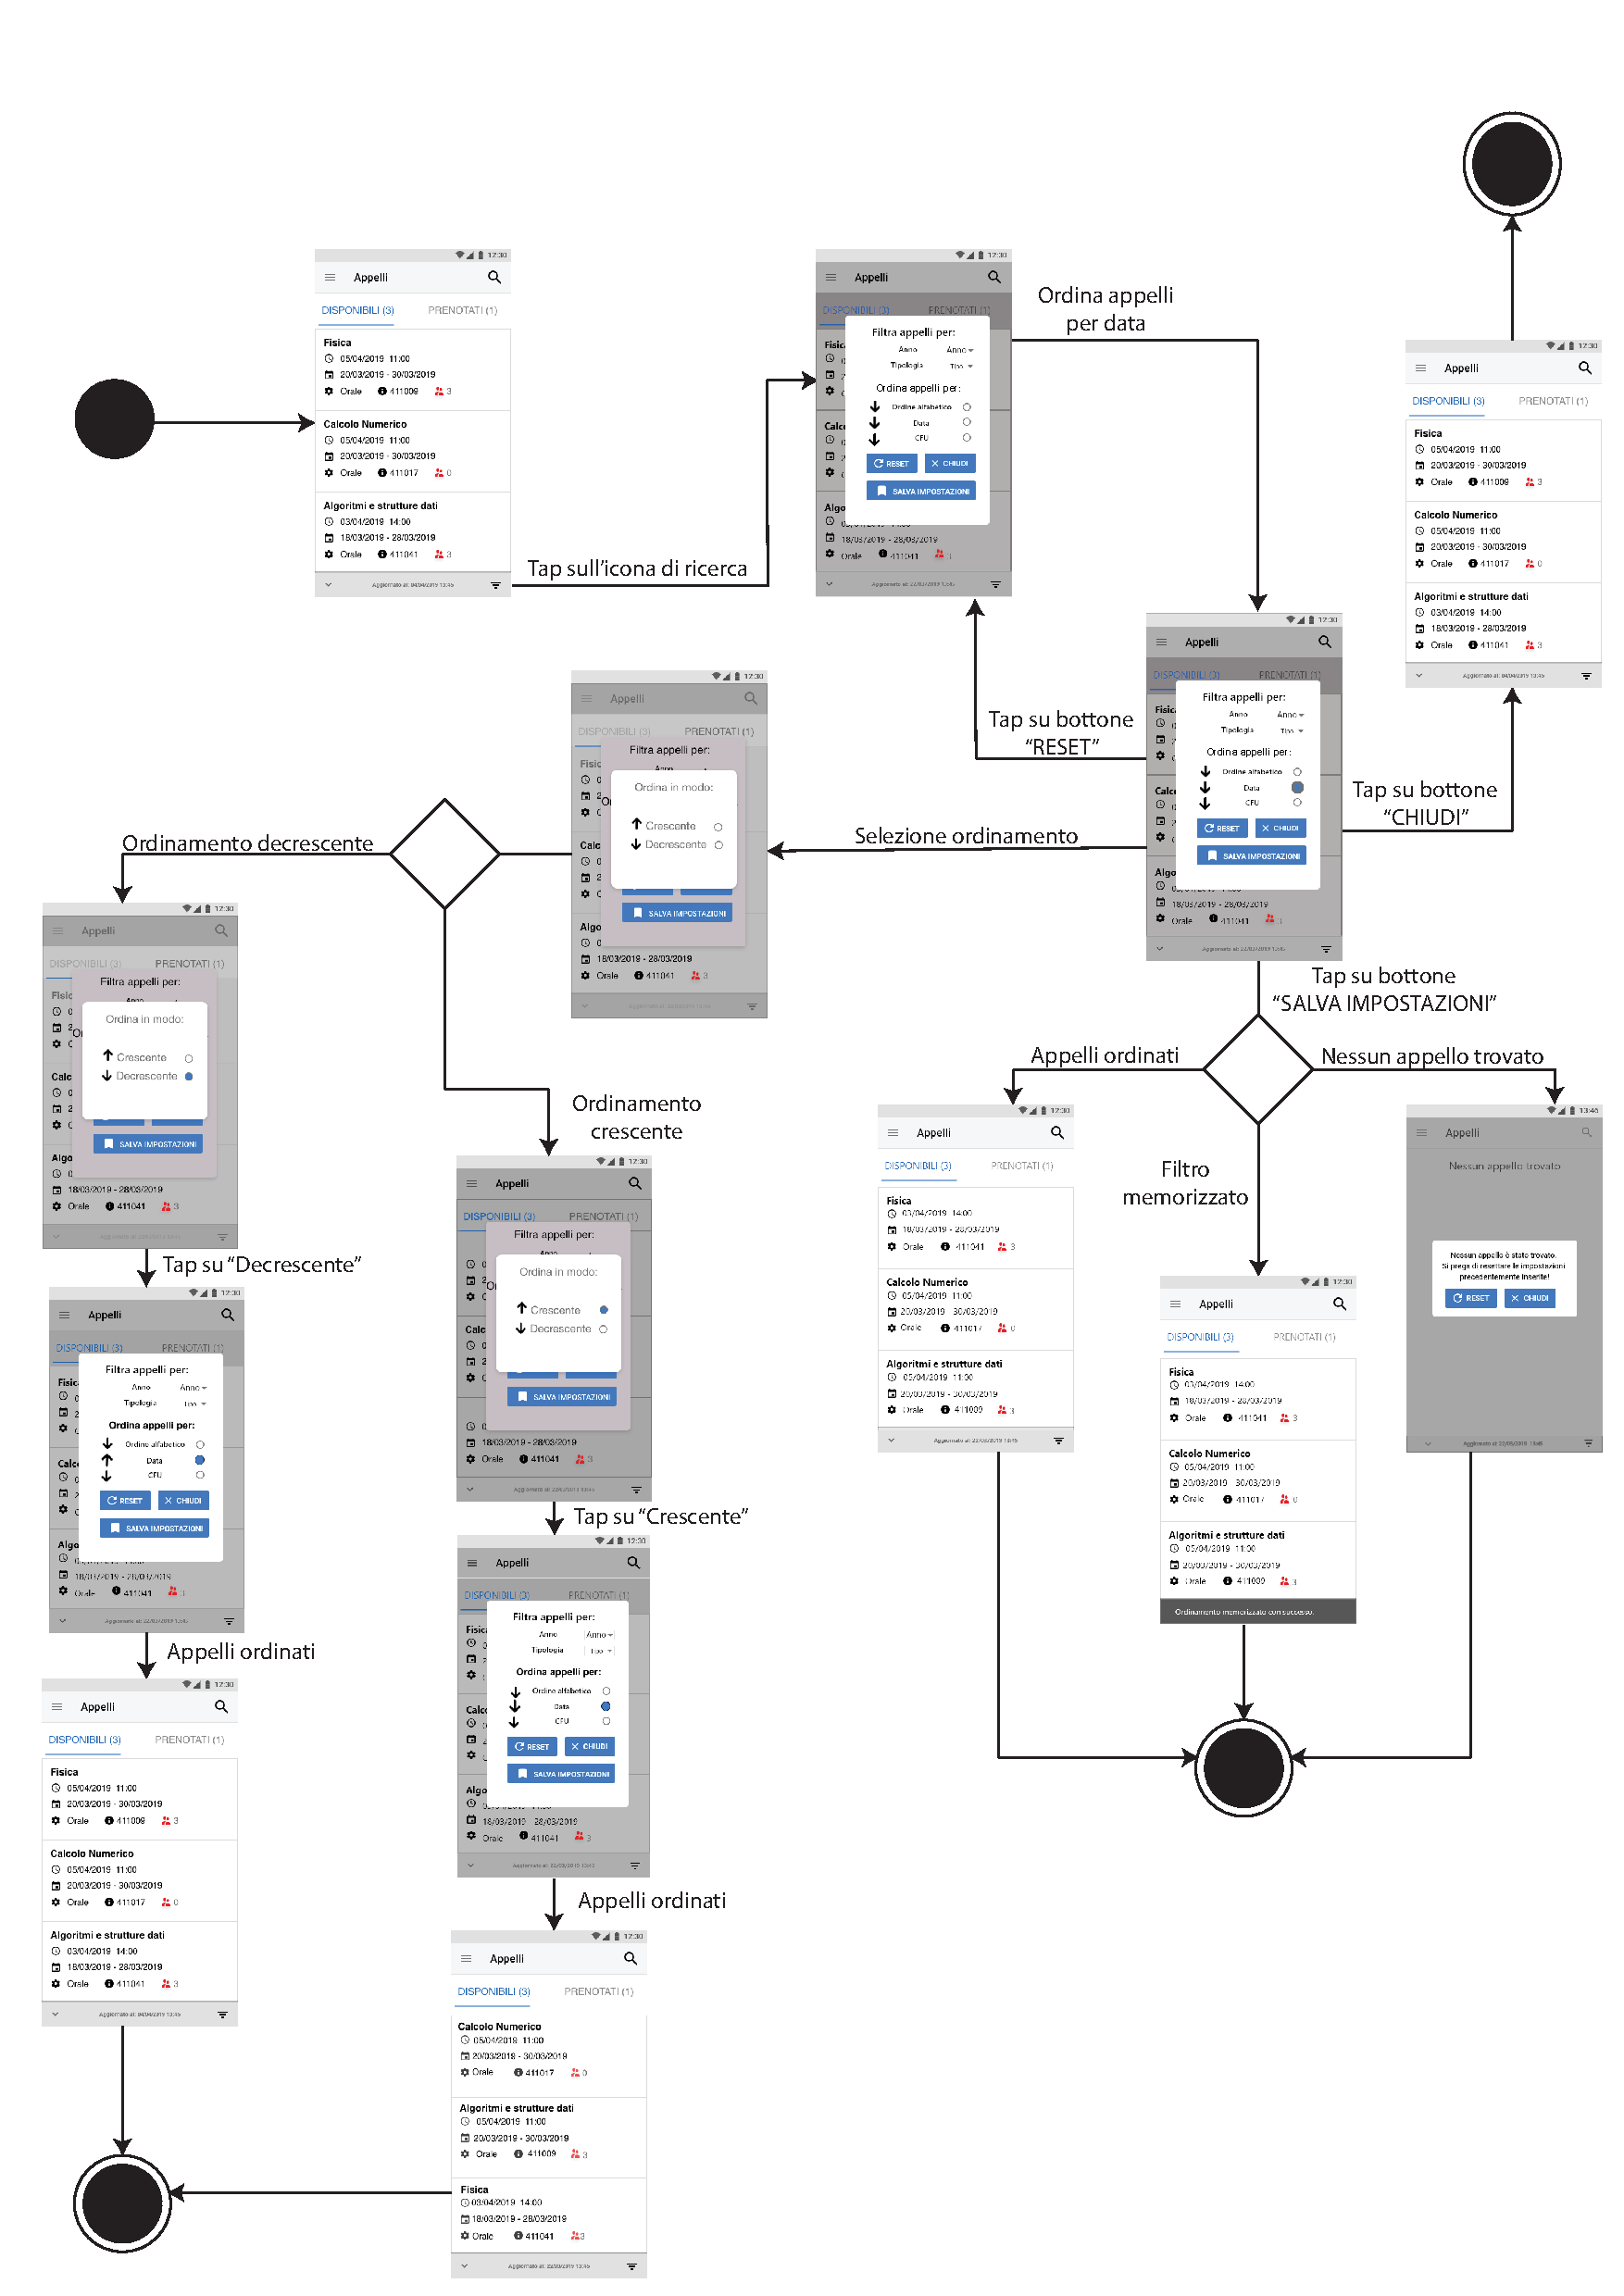
\includegraphics[width=6in]{imgs/gruppo1/activity_diagrams/AD10_ordina_appelli.pdf}
	\caption{Activity Diagram - Ordina appelli disponibili con memorizzazione}
	\label{diag:ordinaAppelliDisponibiliConMemAD}
\end{figure}
\newpage

%\paragraph{Prenota appello }
\begin{figure}
	\centering
	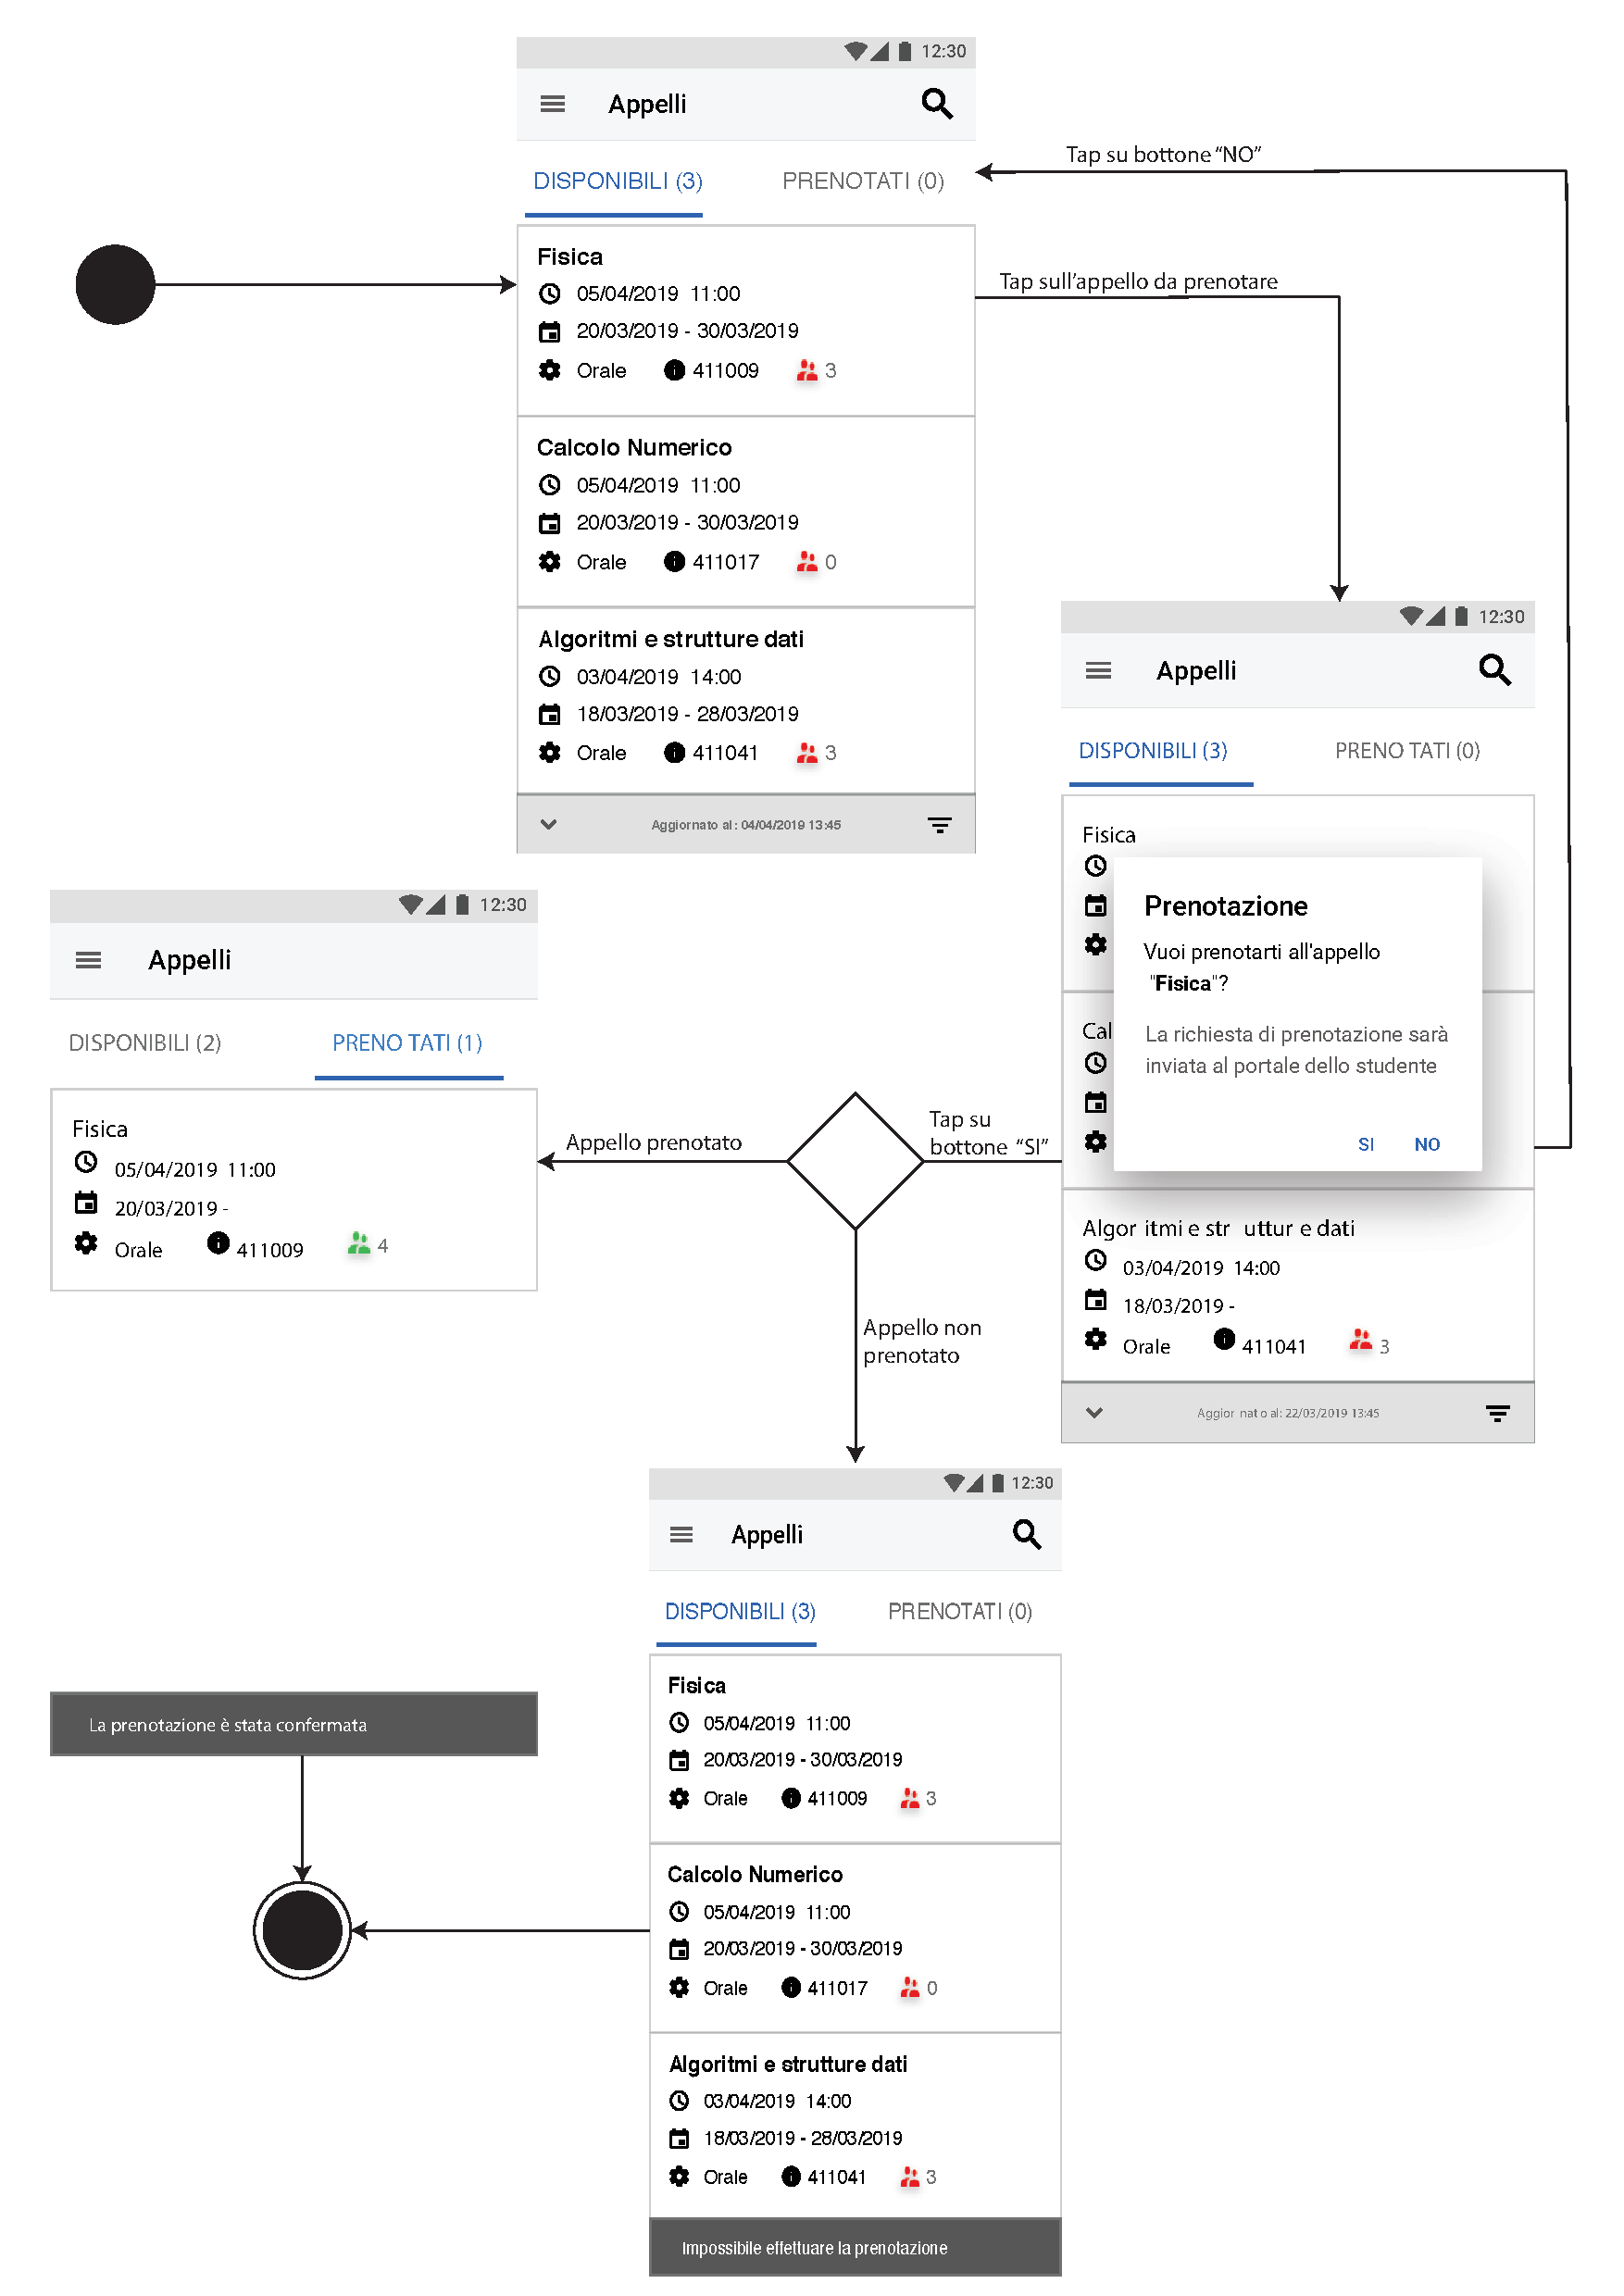
\includegraphics[width=6in]{imgs/gruppo1/activity_diagrams/AD11_prenota_apppello.pdf}
	\caption{Activity Diagram - Prenota appello}
	\label{diag:prenotaAppelloAD}
\end{figure}
\newpage

%\paragraph{Cancella prenotazione}
\begin{figure}
	\centering
	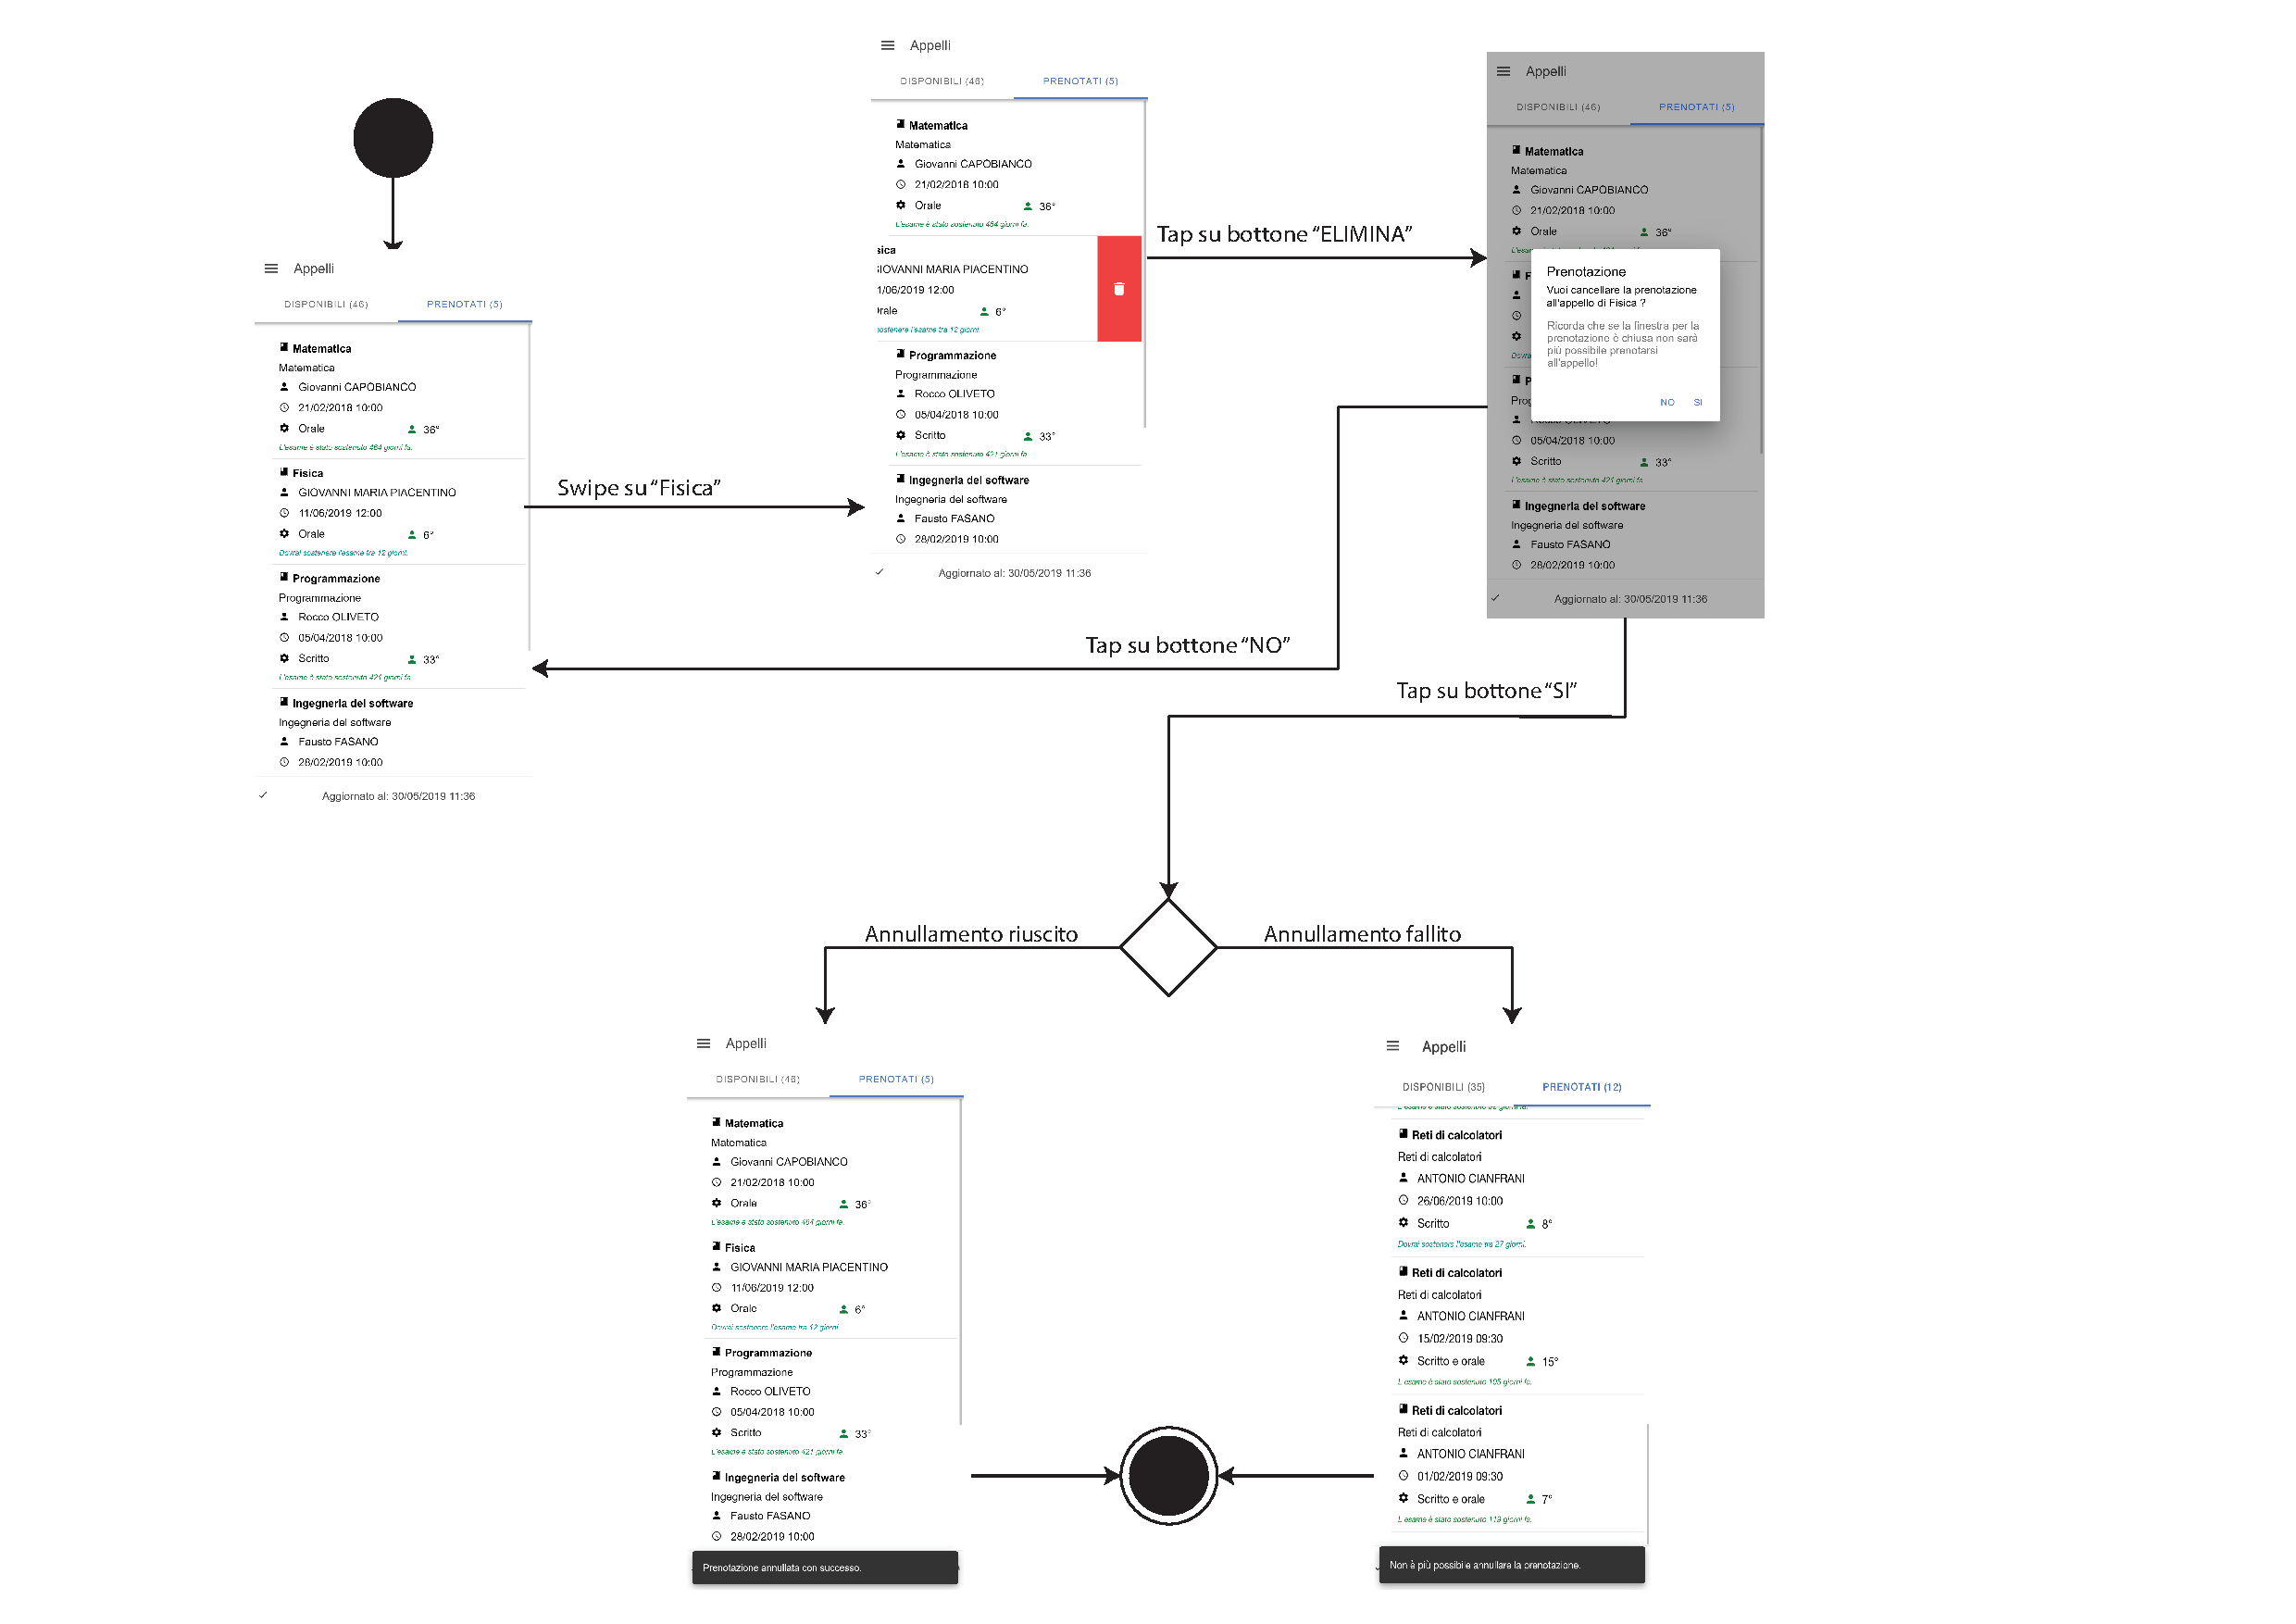
\includegraphics[width=6in]{imgs/gruppo1/activity_diagrams/AD12_cancella_prenotazione.pdf}
<<<<<<< HEAD
	\caption{Activity Diagram - Cancella Prenotazione}
	\label{diag:cancellaPrenotazioneAD}
\end{figure}

\clearpage
\subsection{Funzionalità Gestione materiale didattico}

%\paragraph{Visualizza elenco file}
\begin{figure}
	\centering
	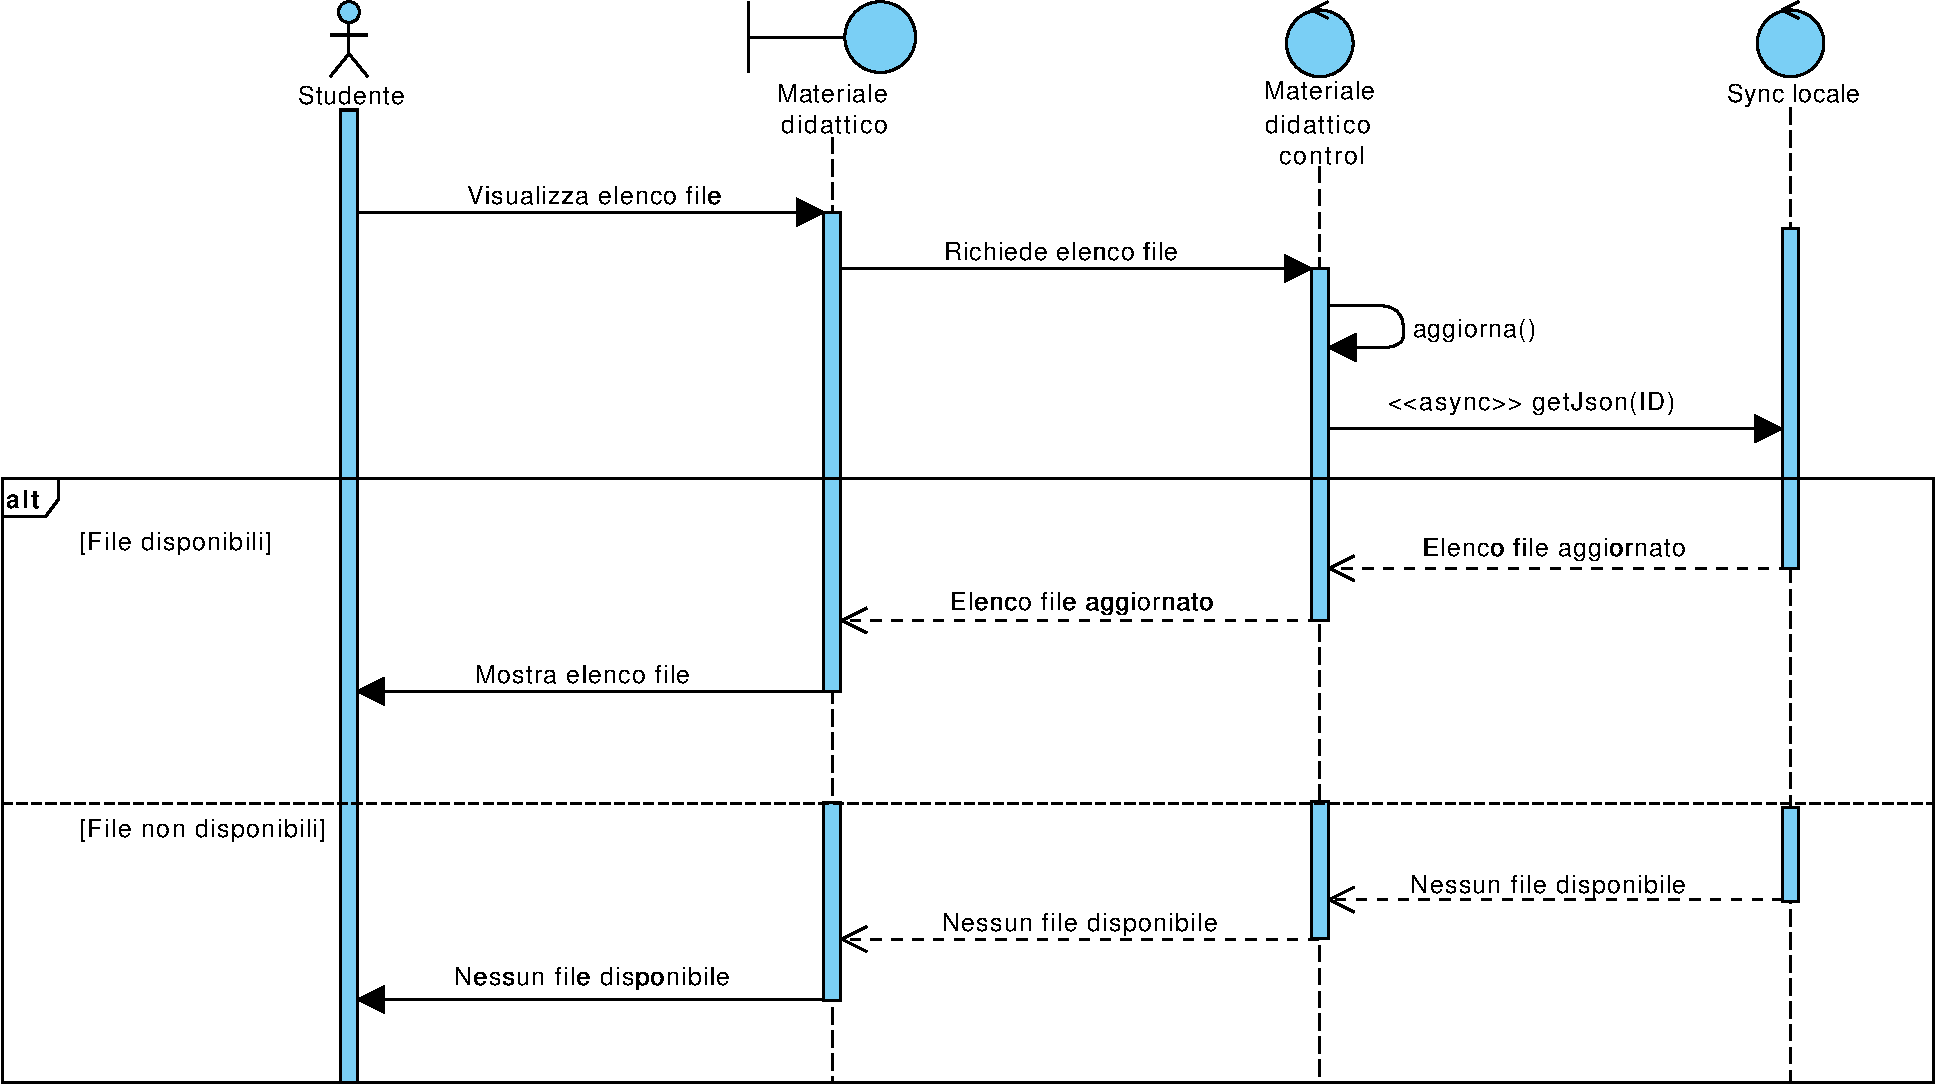
\includegraphics[width=6.5in]{imgs/gruppo1/sequence_diagrams/SD13_visualizza_elenco_file.pdf}
	\caption{Sequence Diagram - Visualizza elenco file}
	\label{diag:visualizzaElencoFileSD}
\end{figure}

%% 8.5.14 - Ricerca file %
\paragraph{Ricerca file}
\begin{figure}
	\centering
	\includegraphics[width=6.5in]{imgs/gruppo1/sequence_diagrams/SD14_ricerca_file.pdf}
	\caption{Sequence Diagram - Ricerca file}
	\label{diag:ricercaFileSD}
\end{figure}
\newpage

%\paragraph{Visualizza dettagli file}
\begin{figure}
	\centering
	\includegraphics[width=6.5in]{imgs/gruppo1//sequence_diagrams/SD15_visualizza_dettagli_file.pdf}
	\caption{Sequence Diagram - Visualizza dettagli file}
	\label{diag:visualizzaDettagliFileSD}
\end{figure}

%\paragraph{Apri file}
\begin{figure}
	\centering
	\includegraphics[width=6.5in]{imgs/gruppo1/sequence_diagrams/SD16_apri_file.pdf}
	\caption{Sequence Diagram - Apri file}
	\label{diag:apriFileSD}
\end{figure}
\newpage

%\paragraph{Rimuovi  file}
\begin{figure}
	\centering
	\includegraphics[width=6.5in]{imgs/gruppo1/sequence_diagrams/SD17_rimuovi_file.pdf}
	\caption{Sequence Diagram - Rimuovi file}
	\label{diag:rimuoviFileSD}
\end{figure}

\clearpage
\subsection{Funzionalità orario}

\subsubsection{Gestione primo avvio}

Giulio, dopo aver selezionato la sezione “orario” dalla voce del menu, potrà spuntare, da una lista di corsi, quelli che vuole seguire. Confermerà la selezione premendo l’apposito tasto “OK”. Da questo momento in poi Giulio potrà visualizzare l’orario costituito dai corsi scelti. 

\subsubsection{Modifica orario}

Giulio modificherà l’orario del proprio anno accademico spuntando la lista dei corsi che vuole seguire. Una volta confermata la modifica, lo studente visualizzerà l’orario aggiornato. 

\subsubsection{Visualizza orario}

Dopo il primo avvio dell’orario, selezionando la sezione “orario” dalla voce del menu, Giulio visualizzerà l’orario.
\subsection{Funzionalità notifiche}

Diagramma di sequenza: Vedi Figura~\vref{fig:seq-diagr-notifiche}.

\begin{figure}
	\centering
	\includegraphics[width=0.85\textwidth]{imgs/gruppo2/sequence-notifiche}
	\caption{Sequence diagram - Notifiche}
	\label{fig:seq-diagr-notifiche}
\end{figure}

\clearpage
\subsection{Funzionalità chat}

\paragraph{CUS1 - Visualizza canale \\}

Lo \emph{Studente}, una volta selezionata la voce \emph{“chat”} dal \emph{menù} dell’app \emph{Studenti Unimol},  seleziona una \emph{chat} specifica della lista e visualizza i messaggi presenti nel canale di discussione della stessa. Nel caso in cui vi sia l’assenza di connessione viene visualizzata l’ultima copia salvata in locale del canale qualora essa sia presente.
\begin{table}
	\small % Dimensione testo piccola
	\label{CUS1 - Visualizza canale}
	\begin{tabular}{| p{\useCaseLeft} | p{\useCaseNum} | p{\useCaseTwoCol} | p{\useCaseTwoCol} |}
		\hline
		\textbf{Nome caso d'uso} & \multicolumn{3}{p{\useCaseMulticol} |}{\textbf{CUS 1 - Visualizza canale}} \\
		\hline
		\textbf{Attori partecipanti} & \multicolumn{3}{p{\useCaseMulticol} |}{Inizializzato da \textbf{\emph{Studente}.}} \\
		\hline
		\textbf{Condizioni d'ingresso} & \multicolumn{3}{p{\useCaseMulticol} |}{Lo \emph{Studente} seleziona la voce \emph{“chat”} dal \emph{menù} dell’\emph{app Studenti Unimol}.} \\
		\hline
		\textbf{Flusso degli eventi} & \textbf{\#} & \textbf{\emph{Studente}} & \textbf{Sistema} \\
		\hline
		\textbf{} & \textbf{1} & \textbf{} & Mostra l’\emph{home-chat} con le relative \emph{chat}; \\
		\hline
		\textbf{} & \textbf{2} & Seleziona la \emph{chat} desiderata; & \textbf{} \\
		\hline
		\textbf{} & \textbf{3} & \textbf{} & Mostra il canale di discussione di \emph{default} della \emph{chat}; \\
		\hline
		\textbf{} & \textbf{4} & Seleziona un canale di discussione alternativo; & \\
		\hline
		\textbf{} & \textbf{5} & \textbf{} & Mostra il canale di discussione selezionato; \\
		\hline
		\textbf{Eccezioni} & \multicolumn{3}{p{\useCaseMulticol} |}{1.1 - 3.1 - 5.1 Nessuna risposta dal \emph{server}: viene visualizzato un messaggio di errore; \newline1.2 - 3.2 - 5.2  Connessione assente: il sistema restituisce l’ultima copia salvata in locale; \newline 1.3 - 3.3 - 5.3 Copia non presente: viene visualizzato un messaggio di errore;} \\
		\hline
		\textbf{Condizioni d'uscita} & \multicolumn{3}{p{\useCaseMulticol} |}{Lo \emph{Studente} visualizza il canale correttamente.} \\
		\hline
	\end{tabular}
	\caption{CUS1 - Visualizza canale}
\end{table}

\newpage
	\paragraph{CUS2 - Invio messaggio \\}

Lo \emph{Studente}, all’interno di un canale di discussione, invia un messaggio selezionando l’apposito spazio dedito alla scrittura. Una volta digitato il testo del messaggio e selezionato il pulsante di invio, il sistema lo mostra nel canale di discussione. \\
\begin{table}

	\small % Dimensione testo piccola
	\label{CUS2 - Invio messaggio}
	\begin{tabular}{| p{\useCaseLeft} | p{\useCaseNum} | p{\useCaseTwoCol} | p{\useCaseTwoCol} |}
		\hline
		\textbf{Nome caso d'uso} & \multicolumn{3}{p{\useCaseMulticol} |}{\textbf{CUS2 - Invio messaggio}} \\
		\hline
		\textbf{Attori partecipanti} & \multicolumn{3}{p{\useCaseMulticol} |}{Inizializzato da \textbf{\emph{Studente}.}} \\
		\hline
		\textbf{Condizioni d'ingresso} & \multicolumn{3}{p{\useCaseMulticol} |}{Lo \emph{Studente} seleziona il canale di discussione in cui vuole inviare il messaggio.} \\
		\hline
		\textbf{Flusso degli eventi} & \textbf{\#} & \textbf{\emph{Studente}} & \textbf{Sistema} \\
		\hline
		\textbf{} & \textbf{1} & Seleziona la casella di testo, digita il messaggio ed invia; & \textbf{} \\
		\hline
		\textbf{} & \textbf{2} & \textbf{} & Riceve il messaggio e lo mostra nella \emph{chat}; \\
		\hline
		\textbf{Eccezioni} & \multicolumn{3}{p{\useCaseMulticol} |}{1.1 Connessione assente: il messaggio viene messo in coda e inviato quando sarà disponibile la connessione; \newline2.1 Nessuna risposta dal \emph{server}: viene visualizzato un messaggio di errore;} \\
		\hline
		\textbf{Condizioni d'uscita} & \multicolumn{3}{p{\useCaseMulticol} |}{Lo \emph{Studente} visualizza il messaggio nel canale della \emph{chat}.} \\
		\hline
	\end{tabular}
	\caption{CUS2 - Invio messaggio}
\end{table}


\newpage
\paragraph{CUS3 - Invio allegato \\}

Lo \emph{Studente} invia un file che viene mostrato all’interno del canale di discussione, similmente ad un messaggio. \\
	
\begin{table}
	
	\small % Dimensione testo piccola
	\label{CUS3 - Invio allegato}	
	\begin{tabular}{| p{\useCaseLeft} | p{\useCaseNum} | p{\useCaseTwoCol} | p{\useCaseTwoCol} |}
		\hline
		\textbf{Nome caso d'uso} & \multicolumn{3}{p{\useCaseMulticol} |}{\textbf{CUS3 - Invio Allegato}} \\
		\hline
		\textbf{Attori partecipanti} & \multicolumn{3}{p{\useCaseMulticol} |}{Inizializzato da \textbf{\emph{Studente}.}} \\
		\hline
		\textbf{Condizioni d'ingresso} & \multicolumn{3}{p{\useCaseMulticol} |}{Lo \emph{Studente} seleziona un canale di discussione.} \\
		\hline
		\textbf{Flusso degli eventi} & \textbf{\#} & \textbf{\emph{Studente}} & \textbf{Sistema} \\
		\hline
		\textbf{} & \textbf{1} & Seleziona il pulsante di scelta allegato; & \textbf{} \\
		\hline
		\textbf{} & \textbf{2} & \textbf{} & Mostra l’elenco dei \emph{file} presenti sul dispositivo dell’utente; \\
		\hline
		\textbf{} & \textbf{3} & Seleziona il \emph{file} da allegare; & \textbf{} \\
		\hline
		\textbf{} & \textbf{4} & \textbf{} & Controlla se l’allegato è idoneo all’invio nel canale di comunicazione e mostra un messaggio di conferma; \\
		\hline
		\textbf{} & \textbf{5} & Invia l’allegato; & \textbf{} \\
		\hline
		\textbf{} & \textbf{6} & \textbf{} & Conferma l’invio dell’allegato; \\
		\hline
		\textbf{Eccezioni} & \multicolumn{3}{p{\useCaseMulticol} |}{2.1 - 4.1 Nessuna risposta dal \emph{server}: viene visualizzato un messaggio di errore; \newline 3.1 Il \emph{file} non è idoneo: viene visualizzato un messaggio di errore; \newline 4.2 Connessione assente: l’allegato viene messo in coda e inviato quando sarà disponibile la connessione;} \\
		\hline
		\textbf{Condizioni d'uscita} & \multicolumn{3}{p{\useCaseMulticol} |}{Il sistema mostra l’allegato nel canale di comunicazione.} \\
		\hline
	\end{tabular}
	\caption{CUS3 - Invio allegato}
\end{table}


\newpage
\paragraph{CUS4 - Rispondi a singolo messaggio \\}
Lo \emph{Studente} visualizza il canale di discussione  desiderato e seleziona il singolo messaggio a cui desidera rispondere. \\
\begin{table}
	\small % Dimensione testo piccola
	\label{CUS4 - Rispondi a singolo messaggio}
	\begin{tabular}{| p{\useCaseLeft} | p{\useCaseNum} | p{\useCaseTwoCol} | p{\useCaseTwoCol} |}
		\hline
		\textbf{Nome caso d'uso} & \multicolumn{3}{p{\useCaseMulticol} |}{\textbf{CUS4 - Rispondi a singolo messaggio}} \\
		\hline
		\textbf{Attori partecipanti} & \multicolumn{3}{p{\useCaseMulticol} |}{Inizializzato da \textbf{\emph{Studente}.}} \\
		\hline
		\textbf{Condizioni d'ingresso} & \multicolumn{3}{p{\useCaseMulticol} |}{Lo \emph{Studente} seleziona il canale di discussione che contiene il messaggio a cui vuole rispondere.} \\
		\hline
		\textbf{Flusso degli eventi} & \textbf{\#} & \textbf{\emph{Studente}} & \textbf{Sistema} \\
		\hline
		\textbf{} & \textbf{1} & Seleziona un messaggio; & \textbf{} \\
		\hline
		\textbf{} & \textbf{2} & \textbf{} & Mostra il \emph{menú}; \\
		\hline
		\textbf{} & \textbf{3} & Seleziona l’opzione di risposta a messaggio; & \textbf{} \\
		\hline
		\textbf{} & \textbf{4} & \textbf{} & Evidenzia il messaggio a cui si vuole rispondere; \\
		\hline
		\textbf{Eccezioni} & \multicolumn{3}{p{\useCaseMulticol} |}{ \textbf{} } \\
		\hline
		\textbf{Condizioni d'uscita} & \multicolumn{3}{p{\useCaseMulticol} |}{Lo \emph{Studente} visualizza il messaggio evidenziato.} \\
		\hline
	\end{tabular}
	\caption{CUS4 - Rispondi a singolo messaggio}
\end{table}


\newpage
\paragraph{CUS5 - Scarica allegato \\}
Lo \emph{Studente} è intenzionato a scaricare un \emph{file} presente nel canale di discussione. \\
\begin{table}
	\small % Dimensione testo piccola
	\label{CUS5 - Scarica allegato}
	
	\begin{tabular}{| p{\useCaseLeft} | p{\useCaseNum} | p{\useCaseTwoCol} | p{\useCaseTwoCol} |}
		\hline
		\textbf{Nome caso d'uso} & \multicolumn{3}{p{\useCaseMulticol} |}{\textbf{CUS5 - Scarica allegato}} \\
		\hline
		\textbf{Attori partecipanti} & \multicolumn{3}{p{\useCaseMulticol} |}{Inizializzato da \textbf{\emph{Studente}.}} \\
		\hline
		\textbf{Condizioni d'ingresso} & \multicolumn{3}{p{\useCaseMulticol} |}{Lo \emph{Studente} seleziona un canale di discussione.} \\
		\hline
		\textbf{Flusso degli eventi} & \textbf{\#} & \textbf{\emph{Studente}} & \textbf{Sistema} \\
		\hline
		\textbf{} & \textbf{1} & Selezione il messaggio dove è presente l’allegato; & \textbf{} \\
		\hline
		\textbf{} & \textbf{2} & \textbf{} & Mostra l’opzione di scaricare l’allegato associato al messaggio selezionato; \\
		\hline
		\textbf{} & \textbf{3} & Seleziona l’opzione per scaricare l’allegato; & \textbf{} \\
		\hline
		\textbf{Eccezioni} & \multicolumn{3}{p{\useCaseMulticol} |}{1.1  Connessione assente: viene visualizzato un messaggio di errore; \newline3.1 Lo \emph{Studente} nega il \emph{download} dell’allegato: l’allegato non viene salvato sul dispositivo;} \\
		\hline
		\textbf{Condizioni d'uscita} & \multicolumn{3}{p{\useCaseMulticol} |}{Il sistema salva il file sul dispositivo.} \\
		\hline
	\end{tabular}
	\caption{CUS5 - Scarica allegato}
\end{table}


\newpage
\paragraph{CUS6 - Segnalazione messaggio \\}
Lo \emph{Studente} dopo aver visualizzato la chat interessata seleziona il messaggio che desidera segnalare. \\
\begin{table}
	\small % Dimensione testo piccola
	\label{CUS6 - Segnalazione messaggio}
	
	\begin{tabular}{| p{\useCaseLeft} | p{\useCaseNum} | p{\useCaseTwoCol} | p{\useCaseTwoCol} |}
		\hline
		\textbf{Nome caso d'uso} & \multicolumn{3}{p{\useCaseMulticol} |}{\textbf{CUS6 - Segnalazione messaggio}} \\
		\hline
		\textbf{Attori partecipanti} & \multicolumn{3}{p{\useCaseMulticol} |}{Inizializzato da \textbf{\emph{Studente}.}} \\
		\hline
		\textbf{Condizioni d'ingresso} & \multicolumn{3}{p{\useCaseMulticol} |}{Lo \emph{Studente} seleziona il canale di discussione che contiene il messaggio che vuole segnalare.} \\
		\hline
		\textbf{Flusso degli eventi} & \textbf{\#} & \textbf{\emph{Studente}} & \textbf{Sistema} \\
		\hline
		\textbf{} & \textbf{1} & Seleziona un messaggio; & \textbf{} \\
		\hline
		\textbf{} & \textbf{2} & \textbf{} & Mostra il \emph{menú}; \\
		\hline
		\textbf{} & \textbf{3} & Seleziona l’opzione “Segnala”; & \textbf{} \\
		\hline
		\textbf{} & \textbf{4} & \textbf{} & Chiede conferma di invio segnalazione; \\
		\hline
		\textbf{} & \textbf{5} & Conferma invio segnalazione; & \textbf{} \\
		\hline
		\textbf{} & \textbf{6} & \textbf{} & Conferma l’avvenuta segnalazione;  \\
		\hline
		\textbf{Eccezioni} & \multicolumn{3}{p{\useCaseMulticol} |}{3.1 Connessione assente: viene visualizzato un messaggio di errore; \newline4.1 - 6.1 Nessuna risposta dal \emph{server}: verrà visualizzato un messaggio di errore;} \\
		\hline
		\textbf{Condizioni d'uscita} & \multicolumn{3}{p{\useCaseMulticol} |}{Il sistema conferma il successo dell’operazione.} \\
		\hline
	\end{tabular}
	\caption{CUS6 - Segnalazione messaggio}
\end{table}


\newpage
\paragraph{CUS7 - Ricerca testo nella chat \\}
Lo \emph{Studente} vuole visualizzare vecchi messaggi seleziona la voce “cerca” nel \emph{menù} interno del canale di discussione, digitando il testo da cercare in un’apposita casella di testo. Il sistema mostra tutti i messaggi che contengono il testo partendo dal più recente. \\
\begin{table}
	\small % Dimensione testo piccola
	\label{CUS7 - Ricerca testo nella chat}
	
	\begin{tabular}{| p{\useCaseLeft} | p{\useCaseNum} | p{\useCaseTwoCol} | p{\useCaseTwoCol} |}
		\hline
		\textbf{Nome caso d'uso} & \multicolumn{3}{p{\useCaseMulticol} |}{\textbf{CUS7 - Ricerca testo nella chat}} \\
		\hline
		\textbf{Attori partecipanti} & \multicolumn{3}{p{\useCaseMulticol} |}{Inizializzato da \textbf{\emph{Studente}.}} \\
		\hline
		\textbf{Condizioni d'ingresso} & \multicolumn{3}{p{\useCaseMulticol} |}{Lo \emph{Studente} seleziona un canale di discussione.} \\
		\hline
		\textbf{Flusso degli eventi} & \textbf{\#} & \textbf{\emph{Studente}} & \textbf{Sistema} \\
		\hline
		\textbf{} & \textbf{1} & Accede alla sezione \emph{“menù”} del canale di discussione; & \textbf{} \\
		\hline
		\textbf{} & \textbf{2} & \textbf{} & Mostra il \emph{menú}; \\
		\hline
		\textbf{} & \textbf{3} & Seleziona il pulsante di ricerca; & \textbf{} \\
		\hline
		\textbf{} & \textbf{4} & \textbf{} &  Mostra la casella di testo di ricerca; \\
		\hline
		\textbf{} & \textbf{5} & Digita il testo da cercare; & \textbf{} \\
		\hline
		\textbf{} & \textbf{6} & \textbf{} & Evidenzia il testo cercato nei messaggi, mostrando prima il più recente;\\
		\hline
		\textbf{} & \textbf{7} & Scorre i messaggi fino a trovare quello ricercato; & \textbf{} \\
		\hline
		\textbf{Eccezioni} & \multicolumn{3}{p{\useCaseMulticol} |}{2.1 - 4.1 - 6.1  Nessuna risposta dal \emph{server}: viene visualizzato un messaggio di errore; \newline6.2 Il testo cercato non è presente: viene visualizzato un messaggio di notifica;} \\
		\hline
		\textbf{Condizioni d'uscita} & \multicolumn{3}{p{\useCaseMulticol} |}{Il sistema evidenzia i messaggi che contengono il testo cercato.} \\
		\hline
	\end{tabular}
	\caption{CUS7 - Ricerca testo nella chat}
\end{table}


\newpage
\paragraph{CUS8 - Tag membro in messaggio \\}
Lo \emph{Studente} che si trova all’interno di un canale di discussione ha la possibilitá di richiamare l’attenzione di uno specifico membro durante la digitazione di un messaggio. Lo studente digita il nome del membro preceduto da un carattere speciale (@). Il membro selezionato viene avvisato tramite una notifica diretta. \\
\begin{table}
	\small % Dimensione testo piccola
	\label{CUS8 - Tag membro in messaggio}
	
	\begin{tabular}{| p{\useCaseLeft} | p{\useCaseNum} | p{\useCaseTwoCol} | p{\useCaseTwoCol} |}
		\hline
		\textbf{Nome caso d'uso} & \multicolumn{3}{p{\useCaseMulticol} |}{\textbf{CUS8 - Tag membro in messaggio}} \\
		\hline
		\textbf{Attori partecipanti} & \multicolumn{3}{p{\useCaseMulticol} |}{Inizializzato da \textbf{\emph{Studente}.}} \\
		\hline
		\textbf{Condizioni d'ingresso} & \multicolumn{3}{p{\useCaseMulticol} |}{Lo \emph{Studente} seleziona un canale di discussione.} \\
		\hline
		\textbf{Flusso degli eventi} & \textbf{\#} & \textbf{\emph{Studente}} & \textbf{Sistema} \\
		\hline
		\textbf{} & \textbf{1} & Seleziona la  casella di testo quindi digita il nome di un membro preceduto dal carattere speciale; & \textbf{} \\
		\hline
		\textbf{} & \textbf{2} & \textbf{} & Mostra la lista di utenti che corrispondono al nome inserito; \\
		\hline
		\textbf{} & \textbf{3} & Seleziona il membro da taggare; & \textbf{} \\
		\hline
		\textbf{Eccezioni} & \multicolumn{3}{p{\useCaseMulticol} |}{1.1 Lo  \emph{Studente} digita il nome errato: il testo digitato viene inserito come messaggio di testo;} \\
		\hline
		\textbf{Condizioni d'uscita} & \multicolumn{3}{p{\useCaseMulticol} |}{Il sistema mostra il messaggio contenente il  \emph{tag} all’interno della casella di testo.} \\
		\hline
	\end{tabular}
	\caption{CUS8 - Tag membro in messaggio}
\end{table}


\newpage
\paragraph{CUS9 - Gestisci notifiche chat \\}
Lo \emph{Studente} che si trova all’interno di una \emph{chat} ha la possibilitá di accedere al \emph{menù} e gestire le notifiche ovvero di attivarle o disattivarle in base alle sue preferenze. \\
\begin{table}
	\small % Dimensione testo piccola
	\label{CUS9 - Gestisci notifiche chat}
	
	\begin{tabular}{| p{\useCaseLeft} | p{\useCaseNum} | p{\useCaseTwoCol} | p{\useCaseTwoCol} |}
		\hline
		\textbf{Nome caso d'uso} & \multicolumn{3}{p{\useCaseMulticol} |}{\textbf{CUS9 - Gestisci notifiche chat}} \\
		\hline
		\textbf{Attori partecipanti} & \multicolumn{3}{p{\useCaseMulticol} |}{Inizializzato da \textbf{\emph{Studente}.}} \\
		\hline
		\textbf{Condizioni d'ingresso} & \multicolumn{3}{p{\useCaseMulticol} |}{Lo \emph{Studente} seleziona un canale di discussione.} \\
		\hline
		\textbf{Flusso degli eventi} & \textbf{\#} & \textbf{\emph{Studente}} & \textbf{Sistema} \\
		\hline
		\textbf{} & \textbf{1} & Accede alla sezione \emph{menú} del canale di discussione; & \textbf{} \\
		\hline
		\textbf{} & \textbf{2} & \textbf{} & Mostra il \emph{menú}; \\
		\hline
		\textbf{} & \textbf{3} & Seleziona il pulsante per attivare/disattivare le notifiche della \emph{chat}; & \textbf{} \\
		\hline
		\textbf{Eccezioni} & \multicolumn{3}{p{\useCaseMulticol} |}{3.1  Connessione assente: viene visualizzato un messaggio di errore; \newline 3.2  Nessuna risposta dal \emph{server}: viene visualizzato un messaggio di errore;} \\
		\hline
		\textbf{Condizioni d'uscita} & \multicolumn{3}{p{\useCaseMulticol} |}{Il sistema cambia lo stato delle notifiche della \emph{chat}.} \\
		\hline
	\end{tabular}
	\caption{CUS9 - Gestisci notifiche chat}
\end{table}


\newpage
\paragraph{CUS10 - Selezione \emph{emoji} \\}
Lo \emph{Studente} che si trova all’interno di un canale di discussione ha la possibilitá di scegliere una o piú \emph{emoji} tra quelle disponibili. \\
\begin{table}
	\small % Dimensione testo piccola
	\label{CUS10 - Selezione emoji}
	
	\begin{tabular}{| p{\useCaseLeft} | p{\useCaseNum} | p{\useCaseTwoCol} | p{\useCaseTwoCol} |}
		\hline
		\textbf{Nome caso d'uso} & \multicolumn{3}{p{\useCaseMulticol} |}{\textbf{CUS10 - Selezione \emph{emoji}}} \\
		\hline
		\textbf{Attori partecipanti} & \multicolumn{3}{p{\useCaseMulticol} |}{Inizializzato da \textbf{\emph{Studente}.}} \\
		\hline
		\textbf{Condizioni d'ingresso} & \multicolumn{3}{p{\useCaseMulticol} |}{Lo \emph{Studente} seleziona un canale di discussione.} \\
		\hline
		\textbf{Flusso degli eventi} & \textbf{\#} & \textbf{\emph{Studente}} & \textbf{Sistema} \\
		\hline
		\textbf{} & \textbf{1} & Seleziona l’icona \emph{emoji}; & \textbf{} \\
		\hline
		\textbf{} & \textbf{2} & \textbf{} & Mostra una finestra con le \emph{emoji} disponibili; \\
		\hline
		\textbf{} & \textbf{3} & Seleziona una o piú \emph{emoji}; & \textbf{} \\
		\hline
		\textbf{} & \textbf{4} & \textbf{} & Il sistema inserisce l’\emph{emoji} nel messaggio; \\
		\hline
		\textbf{Eccezioni} & \multicolumn{3}{p{\useCaseMulticol} |}{ \textbf{} } \\
		\hline
		\textbf{Condizioni d'uscita} & \multicolumn{3}{p{\useCaseMulticol} |}{Lo \emph{Studente} visualizza il messaggio contenente le \emph{emoji} selezionate.} \\
		\hline
	\end{tabular}
	\caption{CUS10 - Selezione \emph{emoji}}
\end{table}


\newpage
\paragraph{CUS11 - Visualizza elenco membri chat \\}
Lo \emph{Studente} visualizza il numero dei partecipanti al canale di discussione e l’elenco contenente l’\emph{username} degli stessi. Nel caso in cui vi sia l’assenza di connessione viene visualizzata l’ultima copia salvata in locale dell’elenco dei partecipanti al canale qualora essa sia presente. \\
\begin{table}
	\small % Dimensione testo piccola
	\label{CUS11 - Visualizza elenco membri chat}
	
	\begin{tabular}{| p{\useCaseLeft} | p{\useCaseNum} | p{\useCaseTwoCol} | p{\useCaseTwoCol} |}
		\hline
		\textbf{Nome caso d'uso} & \multicolumn{3}{p{\useCaseMulticol} |}{\textbf{CUS11 - Visualizza elenco membri chat}} \\
		\hline
		\textbf{Attori partecipanti} & \multicolumn{3}{p{\useCaseMulticol} |}{Inizializzato da \textbf{\emph{Studente}.}} \\
		\hline
		\textbf{Condizioni d'ingresso} & \multicolumn{3}{p{\useCaseMulticol} |}{Lo \emph{Studente} seleziona un canale di discussione.} \\
		\hline
		\textbf{Flusso degli eventi} & \textbf{\#} & \textbf{\emph{Studente}} & \textbf{Sistema} \\
		\hline
		\textbf{} & \textbf{1} & Seleziona il nome del canale di discussione; & \textbf{} \\
		\hline
		\textbf{} & \textbf{2} & \textbf{} & Mostra il numero dei membri del canale di discussione e l’elenco dei loro nomi; \\
		\hline
		\textbf{Eccezioni} & \multicolumn{3}{p{\useCaseMulticol} |}{2.1 Nessuna risposta dal \emph{server}: viene visualizzato un messaggio di errore; \newline2.2 Connessione assente: il sistema restituisce l’ultima copia salvata in locale; \newline2.3 Copia non presente: viene visualizzato un messaggio di errore;} \\
		\hline
		\textbf{Condizioni d'uscita} & \multicolumn{3}{p{\useCaseMulticol} |}{Lo \emph{Studente} visualizza l’elenco dei membri del canale di discussione.} \\
		\hline
	\end{tabular}
	\caption{CUS11 - Visualizza elenco membri chat}
\end{table}

\paragraph{CUE1 - Connessione assente \\}
Lo \emph{Studente} effettua un’operazione che richiede connessione alla rete ma quest’ultima non è disponibile pertanto visualizza un messaggio d’errore. \\
\begin{table}
	\small % Dimensione testo piccola
	\label{CUE1 - Connessione assente}
	\begin{tabular}{| p{\useCaseLeft} | p{\useCaseNum} | p{\useCaseTwoCol} | p{\useCaseTwoCol} |}
		\hline
		\textbf{Nome caso d'uso} & \multicolumn{3}{p{\useCaseMulticol} |}{\textbf{CUE1 - Connessione assente}} \\
		\hline
		\textbf{Attori partecipanti} & \multicolumn{3}{p{\useCaseMulticol} |}{Inizializzato da \textbf{Sistema}, partecipa \textbf{\emph{Studente}.}} \\
		\hline
		\textbf{Condizioni d'ingresso} & \multicolumn{3}{p{\useCaseMulticol} |}{Lo \emph{Studente} effettua un’operazione che richiede connessione alla rete.} \\
		\hline
		\textbf{Flusso degli eventi} & \textbf{\#} & \textbf{\emph{Studente}} & \textbf{Sistema} \\
		\hline
		\textbf{} & \textbf{1} & \textbf{} & Mostra un messaggio d’errore; \\
		\hline
		\textbf{Eccezioni} & \multicolumn{3}{p{\useCaseMulticol} |}{ \textbf{} } \\
		\hline
		\textbf{Condizioni d'uscita} & \multicolumn{3}{p{\useCaseMulticol} |}{Lo \emph{Studente} visualizza il messaggio d’errore.} \\
		\hline
	\end{tabular}
	\caption{CUE1 - Connessione assente}
\end{table}


\newpage
\paragraph{CUE2 - Nessuna risposta dal sistema \\}
Lo \emph{Studente} effettua un’operazione che richiede una risposta dal Sistema, ma quest’ultimo non è in grado di soddisfare la richiesta pertanto visualizza un messaggio d’errore. \\
\begin{table}
	\small % Dimensione testo piccola
	\label{CUE2 - Nessuna risposta dal sistema}
	
	
	Lo \emph{Studente} effettua un’operazione che richiede una risposta dal Sistema, ma quest’ultimo non è in grado di soddisfare la richiesta pertanto visualizza un messaggio d’errore. \\
	
	\begin{tabular}{| p{\useCaseLeft} | p{\useCaseNum} | p{\useCaseTwoCol} | p{\useCaseTwoCol} |}
		\hline
		\textbf{Nome caso d'uso} & \multicolumn{3}{p{\useCaseMulticol} |}{\textbf{CUE2 - Nessuna risposta dal sistema}} \\
		\hline
		\textbf{Attori partecipanti} & \multicolumn{3}{p{\useCaseMulticol} |}{Inizializzato da \textbf{Sistema}, partecipa \textbf{\emph{Studente}.}} \\
		\hline
		\textbf{Condizioni d'ingresso} & \multicolumn{3}{p{\useCaseMulticol} |}{Il Sistema riceve un messaggio di errore.} \\
		\hline
		\textbf{Flusso degli eventi} & \textbf{\#} & \textbf{\emph{Studente}} & \textbf{Sistema} \\
		\hline
		\textbf{} & \textbf{1} & \textbf{} & Riscontra un errore e lo inoltra allo \emph{Studente}; \\
		\hline
		\textbf{Eccezioni} & \multicolumn{3}{p{\useCaseMulticol} |}{ \textbf{} } \\
		\hline
		\textbf{Condizioni d'uscita} & \multicolumn{3}{p{\useCaseMulticol} |}{Lo \emph{Studente} visualizza il messaggio d’errore.} \\
		\hline
	\end{tabular}
	\caption{CUE2 - Nessuna risposta dal sistema}
\end{table}

\paragraph{CUD1 - Creazione canale \\}
Il \emph{Docente}, che si trova all'interno di un cnale di discussione accede alla sezione "\emph{menù}" e crea un nuovo canale all'interno di quello attuale in uso, assengando ad esso un nome ed aggiungendo uno o più membri. \\
\begin{table}
	\small % Dimensione testo piccola
	\label{CUD1 - Creazione canale}
	\begin{tabular}{| p{\useCaseLeft} | p{\useCaseNum} | p{\useCaseTwoCol} | p{\useCaseTwoCol} |}
		\hline
		\textbf{Nome caso d'uso} & \multicolumn{3}{p{\useCaseMulticol} |}{\textbf{CUD1 - Creazione canale}} \\
		\hline
		\textbf{Attori partecipanti} & \multicolumn{3}{p{\useCaseMulticol} |}{Inizializzato da \textbf{\emph{Docente}.}} \\ 
		\hline
		\textbf{Condizioni d'ingresso} & \multicolumn{3}{p{\useCaseMulticol} |}{Il \emph{Docente} seleziona un canale di discussione.} \\
		\hline
		\textbf{Flusso degli eventi} & \textbf{\#} & \textbf{\emph{Docente}} & \textbf{Sistema} \\
		\hline
		\textbf{} & \textbf{1} & Accede alla sezione \emph{menù} del canale di discussione; & \textbf{} \\
		\hline
		\textbf{} & \textbf{2} & \textbf{} & Mostra il \emph{menù}; \\
		\hline
		\textbf{} & \textbf{3} & Seleziona la voce di creazione del nuovo canale; & \textbf{} \\
		\hline
		\textbf{} & \textbf{4} & \textbf{} & Chiede l'immissione del nome del nuovo canale; \\
		\hline
		\textbf{} & \textbf{5} & Inserisce il nome del nuovo canale; & \textbf{} \\
		\hline
		\textbf{} & \textbf{6} & \textbf{} & Chiede conferma del nome inserito; \\
		\hline
		\textbf{} & \textbf{7} & Conferma il nome inserito; & \textbf{} \\
		\hline
		\textbf{} & \textbf{8} & \textbf{} & Chiede l'identificativo dei membri da inserire all'interno del canale; \\
		\hline
		\textbf{} & \textbf{9} & Inserisce l'identificativo dei membri da aggiungere al canale; & \textbf{} \\
		\hline
		\textbf{} & \textbf{10} & \textbf{} & Chiede conferma degli identificativi inseriti; \\
		\hline
		\textbf{} & \textbf{11} & Conferma gli identificativi inseriti; & \textbf{} \\
		\hline
		\textbf{} & \textbf{10} & \textbf{} & Conferma la creazione del canale; \\
		\hline
		\textbf{Eccezioni} & \multicolumn{3}{p{\useCaseMulticol} |}{3.1 Connessione assente: il sistema non procede con la creazione canale; \newline 4.1 - 6.1 - 8.1 - 10.1 - 12.1 Nessuna risposta dal \emph{server}: viene visualizzato un messaggio di errore;} \\
		\hline
		\textbf{Condizioni d'uscita} & \multicolumn{3}{p{\useCaseMulticol} |}{Il \emph{Docente} visualizza il canale appena creato.} \\
		\hline
	\end{tabular}
	\caption{CUD1 - Creazione canale}
\end{table}


\newpage
\paragraph{CUD2 - Cancellazione canale \\}
Il \emph{Docente} che si trova all'interno di un canale di discussione accede alla sezione "\emph{menù}" e effettua la cancellazione di uno dei canali presenti all'interno della \emph{chat}. \\
\begin{table}
	\small % Dimensione testo piccola
	\label{CUD2 - Cancellazione canale}
	\begin{tabular}{| p{\useCaseLeft} | p{\useCaseNum} | p{\useCaseTwoCol} | p{\useCaseTwoCol} |}
		\hline
		\textbf{Nome caso d'uso} & \multicolumn{3}{p{\useCaseMulticol} |}{\textbf{CUD2 - Cancellazione canale}} \\
		\hline
		\textbf{Attori partecipanti} & \multicolumn{3}{p{\useCaseMulticol} |}{Inizializzato da \textbf{\emph{Docente}.}} \\ 
		\hline
		\textbf{Condizioni d'ingresso} & \multicolumn{3}{p{\useCaseMulticol} |}{Il \emph{Docente} seleziona un canale di discussione.} \\
		\hline
		\textbf{Flusso degli eventi} & \textbf{\#} & \textbf{\emph{Docente}} & \textbf{Sistema} \\
		\hline
		\textbf{} & \textbf{1} & Accede alla sezione \emph{menù} del canale di discussione; & \textbf{} \\
		\hline
		\textbf{} & \textbf{2} & \textbf{} & Mostra il \emph{menù}; \\
		\hline
		\textbf{} & \textbf{3} & Seleziona la voce di cancellazione del canale; & \textbf{} \\
		\hline
		\textbf{} & \textbf{4} & \textbf{} & Chiede conferma della cancellaizone; \\
		\hline
		\textbf{} & \textbf{5} & Conferma la scelta; & \textbf{} \\
		\hline
		\textbf{} & \textbf{6} & \textbf{} & procede alla cancellazione del canale; \\
		\hline
		\textbf{Eccezioni} & \multicolumn{3}{p{\useCaseMulticol} |}{3.1 Connessione assente: il canale non viene cancellato; \newline E' presente un solo canale di discussione: il canale non viene cancellato; \newline 4.1 - 6.1 Nessuna risposta dal \emph{server}: viene visualizzato un messaggio di errore;} \\
		\hline
		\textbf{Condizioni d'uscita} & \multicolumn{3}{p{\useCaseMulticol} |}{Il \emph{Docente} visualizza i canali attivi.} \\
		\hline
	\end{tabular}
	\caption{CUD2 - Cancellazione canale}
\end{table}


\newpage
\paragraph{CUD3 - Aggiungi membro ad un canale \\}
Il \emph{Docente} che si trova all'interno di un canale di discussione ha la possibilità di aggiungere un nuovo membro ad un canale attraverso il \emph{menù} di modifica che include l'opzione di aggiunta nuovo membro. \\
\begin{table}
	\small % Dimensione testo piccola
	\label{CUD3 - Aggiungi membro ad un canale}
		\begin{tabular}{| p{\useCaseLeft} | p{\useCaseNum} | p{\useCaseTwoCol} | p{\useCaseTwoCol} |}
		\hline
		\textbf{Nome caso d'uso} & \multicolumn{3}{p{\useCaseMulticol} |}{\textbf{CUD3 - Aggiungi membro ad un canale}} \\
		\hline
		\textbf{Attori partecipanti} & \multicolumn{3}{p{\useCaseMulticol} |}{Inizializzato da \textbf{\emph{Docente}.}} \\ 
		\hline
		\textbf{Condizioni d'ingresso} & \multicolumn{3}{p{\useCaseMulticol} |}{Il \emph{Docente} seleziona un canale di discussione.} \\
		\hline
		\textbf{Flusso degli eventi} & \textbf{\#} & \textbf{\emph{Docente}} & \textbf{Sistema} \\
		\hline
		\textbf{} & \textbf{1} & Accede alla sezione \emph{menù} del canale di discussione; & \textbf{} \\
		\hline
		\textbf{} & \textbf{2} & \textbf{} & Mostra il \emph{menù}; \\
		\hline
		\textbf{} & \textbf{3} & Seleziona la voce aggiungi nuovo membro al canale; & \textbf{} \\
		\hline
		\textbf{} & \textbf{4} & \textbf{} & Chiede l'identificativo del membro da aggiungere al canale; \\
		\hline
		\textbf{} & \textbf{5} & Inserisce l'identificativo del membro da aggiungere; & \textbf{} \\
		\hline
		\textbf{} & \textbf{6} & \textbf{} & Chiede conferma dell'identificativo inserito; \\
		\hline
		\textbf{} & \textbf{7} & Conferma i dati inseriti; & \textbf{} \\
		\hline
		\textbf{} & \textbf{8} & \textbf{} & Conferma l'aggiunta del nuovo \emph{Docente}; \\
		\hline
		\textbf{Eccezioni} & \multicolumn{3}{p{\useCaseMulticol} |}{3.1 Connessione assente: il membro non viene aggiunto; \newline 4.1 - 6.1 - 8.1 Nessuna risposta dal \emph{server}: viene visualizzato un messaggio di errore;} \\
		\hline
		\textbf{Condizioni d'uscita} & \multicolumn{3}{p{\useCaseMulticol} |}{Il \emph{Docente} visualizza l'elenco aggiornato dei membri assegnati al canale.} \\
		\hline
	\end{tabular}
	\caption{CUD3 - Aggiungi membro ad un canale}
\end{table}


\newpage
\paragraph{CUD4 - Rimuovi membro ad un canale \\}
Il \emph{Docente} che si trova all'interno di un canale di discussione ha la possibilità di rimuovere un \emph{Docente} o uno \emph{Studente} da un canale attraverso il \emph{menù} di modifica che include l'opzione di rimozione \emph{Docente} o \emph{Studente}. \\
\begin{table}
	\small % Dimensione testo piccola
	\label{CUD4 - Rimuovi membro ad un canale}
	\begin{tabular}{| p{\useCaseLeft} | p{\useCaseNum} | p{\useCaseTwoCol} | p{\useCaseTwoCol} |}
		\hline
		\textbf{Nome caso d'uso} & \multicolumn{3}{p{\useCaseMulticol} |}{\textbf{CUD4 - Rimuovi membro ad un canale}} \\
		\hline
		\textbf{Attori partecipanti} & \multicolumn{3}{p{\useCaseMulticol} |}{Inizializzato da \textbf{\emph{Docente}.}} \\ 
		\hline
		\textbf{Condizioni d'ingresso} & \multicolumn{3}{p{\useCaseMulticol} |}{Il \emph{Docente} seleziona un canale di discussione.} \\
		\hline
		\textbf{Flusso degli eventi} & \textbf{\#} & \textbf{\emph{Docente}} & \textbf{Sistema} \\
		\hline
		\textbf{} & \textbf{1} & Accede alla sezione \emph{menù} del canale di discussione; & \textbf{} \\
		\hline
		\textbf{} & \textbf{2} & \textbf{} & Mostra il \emph{menù}; \\
		\hline
		\textbf{} & \textbf{3} & Seleziona la voce rimuovi membro dal canale; & \textbf{} \\
		\hline
		\textbf{} & \textbf{4} & \textbf{} & Chiede l'immissione dell'identificativo del membro da rimuovere; \\
		\hline
		\textbf{} & \textbf{5} & Inserisce l'identificativo del membro; & \textbf{} \\
		\hline
		\textbf{} & \textbf{6} & \textbf{} & Chiede conferma dell'identificativo inserito; \\
		\hline
		\textbf{} & \textbf{7} & Conferma l'identificativo inserito; & \textbf{} \\
		\hline
		\textbf{} & \textbf{8} & \textbf{} & Conferma la rimozione del membro dal canale; \\
		\hline
		\textbf{Eccezioni} & \multicolumn{3}{p{\useCaseMulticol} |}{3.1 Connessione assente: non viene eliminato il membro dal canale; \newline 4.1 - 6.1 - 8.1 Nessuna risposta dal \emph{server}: viene visualizzato un messaggio di errore;} \\
		\hline
		\textbf{Condizioni d'uscita} & \multicolumn{3}{p{\useCaseMulticol} |}{Il \emph{Docente} visualizza l'elenco aggiornato dei membri assegnati al canale.} \\
		\hline
	\end{tabular}
	\caption{CUD4 - Rimuovi membro ad un canale}
\end{table}


\newpage
\paragraph{CUD5 - Blocca Studente \\}
Il \emph{Docente} ha la possibilità di silenziare uno \emph{Studente}, nel caso in cui ritenga inappropriati alcuni interventi nel canale di comunicazione. Per silenziare si intende impedire l'invio di nuovi messaggi ad un determinato \emph{Studente}. \\
\begin{table}
	\small % Dimensione testo piccola
	\label{CUD5 - Blocca Studente}
	\begin{tabular}{| p{\useCaseLeft} | p{\useCaseNum} | p{\useCaseTwoCol} | p{\useCaseTwoCol} |}
		\hline
		\textbf{Nome caso d'uso} & \multicolumn{3}{p{\useCaseMulticol} |}{\textbf{CUD5 - Blocca Studente}} \\
		\hline
		\textbf{Attori partecipanti} & \multicolumn{3}{p{\useCaseMulticol} |}{Inizializzato da \textbf{\emph{Docente}.}} \\ 
		\hline
		\textbf{Condizioni d'ingresso} & \multicolumn{3}{p{\useCaseMulticol} |}{Il \emph{Docente} seleziona un canale di discussione.} \\
		\hline
		\textbf{Flusso degli eventi} & \textbf{\#} & \textbf{\emph{Docente}} & \textbf{Sistema} \\
		\hline
		\textbf{} & \textbf{1} & Seleziona un messaggio; & \textbf{} \\
		\hline
		\textbf{} & \textbf{2} & \textbf{} & Mostra l'opzione di blocco dello \emph{Studente} associato al messaggio; \\
		\hline
		\textbf{} & \textbf{3} & Conferma il blocco dello \emph{Studente}; & \textbf{} \\
		\hline
		\textbf{} & \textbf{4} & \textbf{} & Blocca lo \emph{Studente} e mostra un messaggio di conferma; \\
		\hline
		\textbf{} & \textbf{1.1} & Seleziona il nome del canale di discussione; & \textbf{} \\
		\hline
		\textbf{} & \textbf{1.2} & \textbf{} & Mostra il numero dei membri della \emph{chat} e l'elenco dei loro nomi; \\
		\hline
		\textbf{} & \textbf{1.3} & Seleziona uno \emph{Studente}; & \textbf{} \\
		\hline
		\textbf{} & \textbf{2.1} & \textbf{} & Mostra l'opzione di blocco dello \emph{Studente}; \\
		\hline
		\textbf{Eccezioni} & \multicolumn{3}{p{\useCaseMulticol} |}{3.1 Il \emph{Docente} non conferma il blocco dello \emph{Studente}: lo \emph{Studente} non viene bloccato \newline Connessione assente: lo \emph{Studente} non viene bloccato; \newline 4.2 Nessuna risposta dal \emph{server}: viene visualizzato un messaggio di errore;} \\
		\hline
		\textbf{Condizioni d'uscita} & \multicolumn{3}{p{\useCaseMulticol} |}{Il sistema blocca lo \emph{Studente scelto}.} \\
		\hline
	\end{tabular}
	\caption{CUD5 - Blocca Studente}
\end{table}


\newpage
\paragraph{CUD6 - Sblocca Studente \\}
Il \emph{Docente} Il Docente ha la possibilità di sbloccare uno Studente precedentemente bloccato  nel caso in cui ritenga opportuno farlo, così da poter permettere nuovamente allo studente di inviare messaggi nel canale di discussione.    \\
\begin{table}
	\small % Dimensione testo piccola
	\label{CUD6 - Sblocca Studentee}
	\begin{tabular}{| p{\useCaseLeft} | p{\useCaseNum} | p{\useCaseTwoCol} | p{\useCaseTwoCol} |}
		\hline
		\textbf{Nome caso d'uso} & \multicolumn{3}{p{\useCaseMulticol} |}{\textbf{CUD6 - Sblocca Studente}} \\
		\hline
		\textbf{Attori partecipanti} & \multicolumn{3}{p{\useCaseMulticol} |}{Inizializzato da \textbf{\emph{Docente}.}} \\ 
		\hline
		\textbf{Condizioni d'ingresso} & \multicolumn{3}{p{\useCaseMulticol} |}{Il \emph{Docente} seleziona un canale di discussione.} \\
		\hline
		\textbf{Flusso degli eventi} & \textbf{\#} & \textbf{\emph{Docente}} & \textbf{Sistema} \\
		\hline
		\textbf{} & \textbf{1} & Seleziona un messaggio; & \textbf{} \\
		\hline
		\textbf{} & \textbf{2} & \textbf{} & Mostra l'opzione di sblocco dello \emph{Studente} associato al messaggio; \\
		\hline
		\textbf{} & \textbf{3} & Conferma lo sblocco dello \emph{Studente}; & \textbf{} \\
		\hline
		\textbf{} & \textbf{4} & \textbf{} & Sblocca lo \emph{Studente} e mostra un messaggio di conferma; \\
		\hline
		\textbf{} & \textbf{1.1} & Seleziona il nome del canale di discussione; & \textbf{} \\
		\hline
		\textbf{} & \textbf{1.2} & \textbf{} & Mostra il numero dei membri della \emph{chat} e l'elenco dei loro nomi; \\
		\hline
		\textbf{} & \textbf{1.3} & Seleziona uno \emph{Studente}; & \textbf{} \\
		\hline
		\textbf{} & \textbf{2.1} & \textbf{} & Mostra l'opzione di sblocco dello \emph{Studente}; \\
		\hline
		\textbf{Eccezioni} & \multicolumn{3}{p{\useCaseMulticol} |}{3.1 Il \emph{Docente} non conferma lo sblocco dello \emph{Studente}: lo \emph{Studente} non viene sbloccato \newline Connessione assente: lo \emph{Studente} non viene sbloccato; \newline 4.2 Nessuna risposta dal \emph{server}: viene visualizzato un messaggio di errore;} \\
		\hline
		\textbf{Condizioni d'uscita} & \multicolumn{3}{p{\useCaseMulticol} |}{Il sistema sblocca lo \emph{Studente scelto}.} \\
		\hline
	\end{tabular}
	\caption{CUD6 - Sblocca Studente}
\end{table}


\newpage
\paragraph{CUP1 - Login \\}
L'\emph{Amministratore} vuole accedere al pannello di amministrazione. L’accesso avviene mediante l’inserimento di una \emph{username} e \emph{password}. Il \emph{login} dovrà verificare in modo sicuro l’identità di chi sta effettuando l’accesso.\\
\begin{table} 
	\small % Dimensione testo piccola
	\label{CUP1-Login}
	
	\begin{tabular}{| p{\useCaseLeft} | p{\useCaseNum} | p{\useCaseTwoCol} | p{\useCaseTwoCol} |}
		\hline
		\textbf{Nome caso d'uso} & \multicolumn{3}{p{\useCaseMulticol} |}{\textbf{CUP1 - \emph{Login}}} \\
		\hline
		\textbf{Attori partecipanti} & \multicolumn{3}{p{\useCaseMulticol} |}{Inizializzato da \textbf{\emph{Amministratore}}.} \\
		\hline
		\textbf{Condizioni d'ingresso} & \multicolumn{3}{p{\useCaseMulticol} |}{L'\emph{Amministratore} ha raggiunto la schermata di \emph{login}.} \\
		\hline
		\textbf{Flusso degli eventi} & \textbf{\#} & \textbf{\emph{Amministratore}} & \textbf{Sistema} \\
		\hline
		\textbf{} & \textbf{1} & Seleziona la voce \emph{login}; & \textbf{}  \\
		\hline
		\textbf{} & \textbf{2} &  \textbf{} & Propone una schermata per l'inserimento dei dati necessari per il \emph{login}, \emph{username} e \emph{password} dell'\emph{Amministratore};\\
		\hline
		\textbf{} & \textbf{3} & Inserisce i dati e sottomette la richiesta; & \textbf{}  \\
		\hline
		\textbf{} & \textbf{4} &  \textbf{} & Controlla che siano stati inseriti i campi e avvia le operazioni di visualizzazione;\\
		\hline
		
		\textbf{Eccezioni} & \multicolumn{3}{p{\useCaseMulticol} |}{1.1 Connessione assente: non viene visualizzata la schermata di \emph{login};
			\newline 2.1 - 4.1 Errore di sistema: non viene effettuato il \emph{login};
			\newline 3.1 Uno o entrambi i campi sono vuoti: non viene effettutato il \emph{login} e viene evidenziato il campo vuoto con un messaggio di errore;\newline 3.2 Le credenziali inserite non sono valide (una o entrambe): non viene effettuato il \emph{login} e viene visualizzato un messaggio che notifica l'errore di inserimento delle credenziali;} \\
		\hline
		\textbf{Condizioni d'uscita} & \multicolumn{3}{p{\useCaseMulticol} |}{L'\emph{Amministratore} visualizza la schermata \emph{home}.} \\
		\hline
	\end{tabular}
	\caption{\textbf{CUP1 - \emph{Login}}}
\end{table}

\newpage
\paragraph{CUP2 - Logout \\}
L'\emph{Amministratore} vuole uscire dal sistema, chiudendo la sessione in modo sicuro.\\
\begin{table}
	%\normalsize % Dimensione testo normale
	\small % Dimensione testo piccola
	\label{CUP2-Logout}
	\begin{tabular}{| p{\useCaseLeft} | p{\useCaseNum} | p{\useCaseTwoCol} | p{\useCaseTwoCol} |}
		\hline
		\textbf{Nome caso d'uso} & \multicolumn{3}{p{\useCaseMulticol} |}{\textbf{CUP2 - \emph{Logout}}} \\
		\hline
		\textbf{Attori partecipanti} & \multicolumn{3}{p{\useCaseMulticol} |}{Inizializzato da \textbf{\emph{Amministratore}}.} \\
		\hline
		\textbf{Condizioni d'ingresso} & \multicolumn{3}{p{\useCaseMulticol} |}{L'\emph{Amministratore} ha effettuato il \emph{login}.} \\
		\hline
		\textbf{Flusso degli eventi} & \textbf{\#} & \textbf{\emph{Amministratore}} & \textbf{Sistema} \\
		\hline
		\textbf{} & \textbf{1} & Seleziona la voce \emph{logout}; & \textbf{}  \\
		\hline
		\textbf{} & \textbf{2} &  \textbf{} & Chiude la sessione disconnettendo l'\emph{Amministratore};\\
		\hline
		\textbf{Eccezioni} & \multicolumn{3}{p{\useCaseMulticol} |}{1.1 Connessione assente: non viene effettuato il \emph{logout};
			\newline 2.1 Chiusura della sessione non corretta: non viene effettuato il \emph{logout};} \\
		\hline
		\textbf{Condizioni d'uscita} & \multicolumn{3}{p{\useCaseMulticol} |}{L'\emph{Amministratore} visualizza la schermata di \emph{login}.} \\
		\hline
	\end{tabular}
	\caption{\textbf{CUP2 - \emph{Logout}}}
\end{table}

\newpage
\paragraph{CUP3 - Ricerca chat \\}
L'\emph{Amministratore}, seleziona una specifica categoria di \emph{chat} e visualizza una schermata relativa alla ricerca, all’interno della quale è possibile cercare una specifica \emph{chat} o un gruppo di \emph{chat}. Tale ricerca, può essere effettuata mediante l’inserimento del nome della \emph{chat} da ricercare, o attraverso l’utilizzo di filtri.\\
\begin{table}
	%\normalsize % Dimensione testo normale
	\small % Dimensione testo piccola
	\label{CUP3- Ricerca chat}
	\begin{tabular}{| p{\useCaseLeft} | p{\useCaseNum} | p{\useCaseTwoCol} | p{\useCaseTwoCol} |}
		\hline
		\textbf{Nome caso d'uso} & \multicolumn{3}{p{\useCaseMulticol} |}{\textbf{CUP3 - Ricerca \emph{chat}}} \\
		\hline
		\textbf{Attori partecipanti} & \multicolumn{3}{p{\useCaseMulticol} |}{Inizializzato da \textbf{\emph{Amministratore}}.} \\
		\hline
		\textbf{Condizioni d'ingresso} & \multicolumn{3}{p{\useCaseMulticol} |}{L'\emph{Amministratore} visualizza la schermata per effettuare una ricerca;} \\
		\hline
		\textbf{Flusso degli eventi} & \textbf{\#} & \textbf{\emph{Amministratore}} & \textbf{Sistema} \\
		\hline
		\textbf{} & \textbf{1} & Seleziona la voce "Ricerca"; & \textbf{}  \\
		\hline
		\textbf{} & \textbf{2} &  \textbf{} & Chiede il testo da cercare;\\
		\hline
		\textbf{} & \textbf{3} & Inserisce il testo da cercare; & \textbf{}  \\
		\hline
		\textbf{} & \textbf{4} &  \textbf{} & Effettua la ricerca e mostra la \emph{chat} desiderata;\\
		\hline
		\textbf{} & \textbf{1.1} & Seleziona il filtro "Dipartimento"; & \textbf{}  \\
		\hline
		\textbf{} & \textbf{2.1} &  \textbf{} & Mostra i dipartimenti;\\
		\hline
		\textbf{} & \textbf{3.1} & Seleziona un dipartimento e procede col selezionare il secondo filtro “Corsi di laurea”;  & \textbf{}  \\
		\hline
		\textbf{} & \textbf{4.1} &  \textbf{} & Mostra i corsi di laurea del  dipartimento precedentemente selezionato;\\
		\hline
		\textbf{} & \textbf{5.1} & Seleziona un corso di laurea e procede col selezionare il terzo filtro “Anno corso”; & \textbf{}  \\
		\hline
		\textbf{} & \textbf{6.1} &  \textbf{} & Mostra la coorte degli anni che individuano un anno accademico di un corso di laurea; \\
		\hline
		\textbf{} & \textbf{7.1} & Seleziona la coorte di un anno accademico e procede con la ricerca;  & \textbf{}  \\
		\hline
		
		\textbf{Eccezioni} & \multicolumn{3}{p{\useCaseMulticol} |}{1.1 Connessione assente: viene visualizzato un messaggio di errore;
			\newline 2.1 - 2.1.1 - 4.1.1 - 6.1.1 Errore di sistema: viene visualizzato un messaggio di errore;
			\newline 4.1 \emph{Chat} non trovata: viene visualizzato un messaggio di errore;} \\
		\hline
		\textbf{Condizioni d'uscita} & \multicolumn{3}{p{\useCaseMulticol} |}{L'\emph{Amministratore} visualizza correttamente la \emph{chat} ricercata, o l'elenco delle \emph{chat} inerenti ai filtri applicati.} \\
		\hline
	\end{tabular}
	\caption{\textbf{CUP3 - Ricerca \emph{chat}}}
\end{table}

\newpage
\paragraph{CUP4 - Visualizza lista chat \\}
L'\emph{Amministratore} vuole selezionare una tipologia di \emph{chat} da visualizzare.
E’ possibile visualizzare la lista delle \emph{chat} studenti e delle \emph{chat} dei corsi, queste ultime suddivise a loro volta in \emph{chat} attive e non attive. La suddivisione garantisce una corretta caratterizzazione e organizzazione delle \emph{chat}.\\
\begin{table}
	%\normalsize % Dimensione testo normale
	\small % Dimensione testo piccola
	\label{CUP4 - Visualizza lista chat}
	\begin{tabular}{| p{\useCaseLeft} | p{\useCaseNum} | p{\useCaseTwoCol} | p{\useCaseTwoCol} |}
		\hline
		\textbf{Nome caso d'uso} & \multicolumn{3}{p{\useCaseMulticol} |}{\textbf{CUP4 - Visualizza lista \emph{chat}}} \\
		\hline
		\textbf{Attori partecipanti} & \multicolumn{3}{p{\useCaseMulticol} |}{Inizializzato da \textbf{\emph{Amministratore}}.} \\
		\hline
		\textbf{Condizioni d'ingresso} & \multicolumn{3}{p{\useCaseMulticol} |}{L'\emph{Amministratore} effettua il \emph{login} e si trova nella schermata principale.} \\
		\hline
		\textbf{Flusso degli eventi} & \textbf{\#} & \textbf{\emph{Amministratore}} & \textbf{Sistema} \\
		\hline
		\textbf{} & \textbf{1} & Seleziona come categoria di \emph{chat} da visualizzare le \emph{chat} degli studenti; & \textbf{}  \\
		\hline
		\textbf{} & \textbf{2} & Effettua la ricerca come da caso d'uso CUP3 Ricerca \emph{chat}; & \textbf{}  \\
		\hline
		\textbf{} & \textbf{3} &  \textbf{} & Mostra l'elenco delle \emph{chat} degli studenti;\\
		\hline
		\textbf{} & \textbf{1.1} & Seleziona come categoria di \emph{chat} da visualizzare le chat relative ai corsi; & \textbf{}  \\
		\hline
		\textbf{} & \textbf{2.1} & Effettua la ricerca come da caso d'uso CUP3 Ricerca \emph{chat}; & \textbf{}  \\
		\hline
		\textbf{} & \textbf{3.1} &  \textbf{} & Mostra la schermata con l'elenco delle \emph{chat} attive;\\
		\hline
		\textbf{} & \textbf{1.1.1} & Seleziona la schermata con l'elenco delle \emph{chat} non attive; & \textbf{}  \\
		\hline
		\textbf{} & \textbf{3.1.1} &  \textbf{} & Mostra l'elenco delle \emph{chat} non attive; \\
		
		\hline
		
		\textbf{Eccezioni} & \multicolumn{3}{p{\useCaseMulticol} |}{1.1 Connessione assente: non viene visualizzata la lista delle \emph{chat};
			\newline 3.1 - 3.1.1 - 3.1.1.1 Errore di sistema: viene visualizzato un messaggio di errore;
		} \\
		\hline
		\textbf{Condizioni d'uscita} & \multicolumn{3}{p{\useCaseMulticol} |}{L'\emph{Amministratore} visualizza la lista delle \emph{chat} ricercate.} \\
		\hline
	\end{tabular}
	\caption{\textbf{CUP4 - Visualizza lista \emph{chat}}}
	\end{table}


\newpage
\paragraph{CUP5 - Abilita chat \\}
L'\emph{Amministratore} visualizza l’elenco delle \emph{chat} di corso non attive e a seguito di una richiesta abilita una specifica \emph{chat}.\\
\begin{table}
	%\normalsize % Dimensione testo normale
	\small % Dimensione testo piccola
	\label{CUP5-Abilita chat}
	
	\begin{tabular}{| p{\useCaseLeft} | p{\useCaseNum} | p{\useCaseTwoCol} | p{\useCaseTwoCol} |}
		\hline
		\textbf{Nome caso d'uso} & \multicolumn{3}{p{\useCaseMulticol} |}{\textbf{CUP5 - Abilita \emph{chat}}} \\
		\hline
		\textbf{Attori partecipanti} & \multicolumn{3}{p{\useCaseMulticol} |}{Inizializzato da \textbf{\emph{Amministratore}}.} \\
		\hline
		\textbf{Condizioni d'ingresso} & \multicolumn{3}{p{\useCaseMulticol} |}{L'\emph{Amministratore} seleziona la categoria corsi, all’interno della quale visualizza le \emph{chat} abilitate.} \\
		\hline
		\textbf{Flusso degli eventi} & \textbf{\#} & \textbf{\emph{Amministratore}} & \textbf{Sistema} \\
		\hline
		\textbf{} & \textbf{1} & Seleziona una \emph{chat} e accede alla sezione abilita \emph{chat}; & \textbf{}  \\
		\hline
		\textbf{} & \textbf{2} &  \textbf{} & Mostra un pannello in cui chiede conferma per abilitare la \emph{chat} selezionata;\\
		\hline
		\textbf{} & \textbf{3} & Conferma l'abilitazione della \emph{chat}; & \textbf{}  \\
		\hline
		\textbf{} & \textbf{4} &  \textbf{} & Abilita la \emph{chat} e inserisce la \emph{chat} attivata all'interno dell'elenco delle \emph{chat} abilitate;\\
		\hline
		
		\textbf{Eccezioni} & \multicolumn{3}{p{\useCaseMulticol} |}{1.1 Connessione assente: viene visualizzato un messaggio di errore;
			\newline 2.1 - 4.1 Errore di sistema: viene visualizzato un messaggio di errore;
		} \\
		\hline
		\textbf{Condizioni d'uscita} & \multicolumn{3}{p{\useCaseMulticol} |}{L'\emph{Amministratore} visualizza la schermata \emph{chat} attive.} \\
		\hline
	\end{tabular}
	\caption{\textbf{CUP5 - Abilita \emph{chat}}}
\end{table}

\newpage
\paragraph{CUP6 - Disabilita chat \\}
L'\emph{Amministratore} visualizza l’elenco delle \emph{chat} di corso attive e a seguito di una richiesta disabilita una specifica \emph{chat}.\\
\begin{table}
	%\normalsize % Dimensione testo normale
	\small % Dimensione testo piccola
	\label{CUP6-Disabilita chat}
	
	\begin{tabular}{| p{\useCaseLeft} | p{\useCaseNum} | p{\useCaseTwoCol} | p{\useCaseTwoCol} |}
		\hline
		\textbf{Nome caso d'uso} & \multicolumn{3}{p{\useCaseMulticol} |}{\textbf{CUP6 - Disabilita \emph{chat}}} \\
		\hline
		\textbf{Attori partecipanti} & \multicolumn{3}{p{\useCaseMulticol} |}{Inizializzato da \textbf{\emph{Amministratore}}.} \\
		\hline
		\textbf{Condizioni d'ingresso} & \multicolumn{3}{p{\useCaseMulticol} |}{L'\emph{Amministratore} seleziona la categoria corsi, all'interno della quale visualizza le \emph{chat} abilitate.} \\
		\hline
		\textbf{Flusso degli eventi} & \textbf{\#} & \textbf{\emph{Amministratore}} & \textbf{Sistema} \\
		\hline
		\textbf{} & \textbf{1} & Seleziona una \emph{chat} e seleziona la voce disabilita \emph{chat};& \textbf{} \\
		\hline
		\textbf{} & \textbf{2} & \textbf{} & Mostra un pannello in cui chiede conferma per disabilitare la \emph{chat} selezionata; \\
		\hline
		\textbf{} & \textbf{3} & Conferma la disabilitazione della \emph{chat};& \textbf{} \\
		\hline
		\textbf{} & \textbf{4} & \textbf{} & Disabilita la \emph{chat} e inserisce la \emph{chat} disattivata all'interno dell'elenco delle \emph{chat} non abilitate; \\
		\hline
		
		\textbf{Eccezioni} & \multicolumn{3}{p{\useCaseMulticol} |}{1.1 Connessione assente: viene visualizzato un messaggio di errore;\newline 2.1 - 4.1 Errore di sistema: viene visualizzato un messaggio di errore;} \\
		\hline
		\textbf{Condizioni d'uscita} & \multicolumn{3}{p{\useCaseMulticol} |}{L'\emph{Amministratore} visualizza la schermata \emph{chat} non attive.} \\
		\hline
	\end{tabular}
	\caption{\textbf{CUP6 - Disabilita \emph{chat}}}
\end{table}

\newpage
\paragraph{CUP7 - Visualizza canale \\}
L'\emph{Amministratore} seleziona una specifica chat da visualizzare.
In quest’ultima, visualizza i canali in cui è suddivisa e, selezionato un opportuno canale, ne visualizza i messaggi in esso contenuti.\\
\begin{table}
	%\normalsize % Dimensione testo normale
	\small % Dimensione testo piccola
	\label{CUP7- Visualizza canale}
	\begin{tabular}{| p{\useCaseLeft} | p{\useCaseNum} | p{\useCaseTwoCol} | p{\useCaseTwoCol} |}
		\hline
		\textbf{Nome caso d'uso} & \multicolumn{3}{p{\useCaseMulticol} |}{\textbf{CUP7 - Visualizza canale}} \\
		\hline
		\textbf{Attori partecipanti} & \multicolumn{3}{p{\useCaseMulticol} |}{Inizializzato da \textbf{\emph{Amministratore}}.} \\
		\hline
		\textbf{Condizioni d'ingresso} & \multicolumn{3}{p{\useCaseMulticol} |}{L'\emph{Amministratore} seleziona una specifica categoria.} \\
		\hline
		\textbf{Flusso degli eventi} & \textbf{\#} & \textbf{\emph{Amministratore}} & \textbf{Sistema} \\
		\hline
		\textbf{} & \textbf{1} & Seleziona la \emph{chat} da visualizzare; & \textbf{} \\
		\hline
		\textbf{} & \textbf{2} & \textbf{} & Mostra la relativa \emph{chat} e i canali in essa contenuti; \\
		\hline
		\textbf{} & \textbf{3} & Seleziona uno specifico canale;& \textbf{} \\
		\hline
		\textbf{} & \textbf{4} & \textbf{} & Mostra la conversazione inerente al canale selezionato; \\
		\hline
		
		\textbf{Eccezioni} & \multicolumn{3}{p{\useCaseMulticol} |}{1.1 Connessione assente: viene visualizzato un messaggio di errore;\newline 2.1 - 4.1 Errore di sistema: viene visualizzato un messaggio di errore;} \\
		\hline
		\textbf{Condizioni d'uscita} & \multicolumn{3}{p{\useCaseMulticol} |}{L'\emph{Amministratore} visualizza il canale selezionato.} \\
		\hline
	\end{tabular}
	\caption{\textbf{CUP7 - Visualizza canale}}
\end{table}

\newpage
\paragraph{CUP8 - Aggiungi canale \\}
L'\emph{Amministratore} vuole creare un nuovo canale all’interno della \emph{chat} al fine di rendere la conversazione quanto più organizzata possibile e di suddividere eventuali moduli e partizionamenti di un corso. Ha quindi la possibilità di aggiungere utenti al canale della \emph{chat} e di scegliere il nome del nuovo canale.\\
\begin{table}
	
	\small % Dimensione testo piccola
	
	\label{CUP8-Aggiungi canale}
	\begin{tabular}{| p{\useCaseLeft} | p{\useCaseNum} | p{\useCaseTwoCol} | p{\useCaseTwoCol} |}
		\hline
		\textbf{Nome caso d'uso} & \multicolumn{3}{p{\useCaseMulticol} |}{\textbf{CUP8 - Aggiungi canale}} \\
		\hline
		\textbf{Attori partecipanti} & \multicolumn{3}{p{\useCaseMulticol} |}{Inizializzato da \textbf{\emph{Amministratore}}.} \\
		\hline
		\textbf{Condizioni d'ingresso} & \multicolumn{3}{p{\useCaseMulticol} |}{L'\emph{Amministratore} seleziona una \emph{chat} attiva.} \\
		\hline
		\textbf{Flusso degli eventi} & \textbf{\#} & \textbf{\emph{Amministratore}} & \textbf{Sistema} \\
		\hline
		\textbf{} & \textbf{1} & Seleziona la voce "Gestione canali"; & \textbf{}  \\
		\hline
		\textbf{} & \textbf{2} &  \textbf{} & Mostra le opzioni per i canali;\\
		\hline
		\textbf{} & \textbf{3} &Seleziona la voce "Crea nuovo canale"; & \textbf{}  \\
		\hline
		\textbf{} & \textbf{4} &  \textbf{} & Mostra le opzioni per il nuovo canale;\\
		\hline
		
		\textbf{} & \textbf{5} & Inserisce il nome del canale e procede; & \textbf{}  \\
		\hline
		\textbf{} & \textbf{6} &  \textbf{} & Mostra la schermata per procedere all'inserimento degli utenti del canale;\\
		\hline
		\textbf{} & \textbf{7} &Inserisce gli utenti che ne fanno parte e procedere selezionando la voce "Aggiungi utenti"; & \textbf{}  \\
		\hline
		\textbf{} & \textbf{8} &  \textbf{} & Mostra la schermata per confermare la creazione del canale;\\
		\hline
		\textbf{} & \textbf{9} & Procede selezionando "Crea canale"; & \textbf{}  \\
		\hline
		\textbf{} & \textbf{10} &  \textbf{} & Crea e mostra il canale all'interno della \emph{chat};\\
		\hline		
		\textbf{Eccezioni} & \multicolumn{3}{p{\useCaseMulticol} |}{1.1 Connessione assente: viene visualizato un messaggio di errore;
			\newline 2.1 - 4.1 - 6.1 - 8.1 Errore di sistema: viene visualizzato un messaggio di errore;
			\newline 6.1 Il canale non viene creato: viene visualizzato un messaggio di errore;} \\
		\hline
		\textbf{Condizioni d'uscita} & \multicolumn{3}{p{\useCaseMulticol} |}{L'\emph{Amministratore} visualizza un messaggio di conferma della creazione del nuovo canale.} \\
		\hline
	\end{tabular}
	\caption{\textbf{CUP8 - Aggiungi canale}}
\end{table}

\newpage
\paragraph{CUP9 - Cancella canale \\}
L'\emph{Amministratore} potrà eliminare un canale esistente qualora ne venga richiesta l’eliminazione.\\
\begin{table}
	%\normalsize % Dimensione testo normale
	\small % Dimensione testo piccola
	\label{CUP9-Cancella canale}
	\begin{tabular}{| p{\useCaseLeft} | p{\useCaseNum} | p{\useCaseTwoCol} | p{\useCaseTwoCol} |}
		\hline
		\textbf{Nome caso d'uso} & \multicolumn{3}{p{\useCaseMulticol} |}{\textbf{CUP9 - Cancella canale}} \\
		\hline
		\textbf{Attori partecipanti} & \multicolumn{3}{p{\useCaseMulticol} |}{Inizializzato da \textbf{\emph{Amministratore}}.} \\
		\hline
		\textbf{Condizioni d'ingresso} & \multicolumn{3}{p{\useCaseMulticol} |}{L'\emph{Amministratore} sleziona una \emph{chat} attiva.} \\
		\hline
		\textbf{Flusso degli eventi} & \textbf{\#} & \textbf{\emph{Amministratore}} & \textbf{Sistema} \\
		\hline
		\textbf{} & \textbf{1} & Seleziona la voce "Gestione canali"; & \textbf{}  \\
		\hline
		\textbf{} & \textbf{2} &  \textbf{} & Mostra le opzioni per i canali;\\
		\hline
		\textbf{} & \textbf{3} &Seleziona la voce "Elimina canale"; & \textbf{}  \\
		\hline
		\textbf{} & \textbf{4} &  \textbf{} & Mostra lista dei canali della \emph{chat};\\
		\hline
		
		\textbf{} & \textbf{5} & Seleziona il canale da eliminare e procede all'eliminazione; & \textbf{}  \\
		\hline
		\textbf{} & \textbf{6} &  \textbf{} & Il sistema elimina il canale selezionato;\\
		\hline
		
		\textbf{Eccezioni} & \multicolumn{3}{p{\useCaseMulticol} |}{1.1 Connessione assente: viene visualizato un messaggio di errore;
			\newline 2.1 - 4.1 - 6.1  Errore di sistema: viene visualizzato un messaggio di errore;
			\newline 4.1 Non ci sono canali nella \emph{chat}: viene visualizzato un messaggio di errore;} \\
		\hline
		\textbf{Condizioni d'uscita} & \multicolumn{3}{p{\useCaseMulticol} |}{L'\emph{Amministratore} visualizza un messaggio di conferma della rimozione del canale.} \\
		\hline
	\end{tabular}
	\caption{\textbf{CUP9 - Cancella canale}}
\end{table}

\newpage
\paragraph{CUP10 - Visualizza lista utenti \\}
L'\emph{Amministratore} vuole visualizzare la lista degli utenti presenti all'interno di un canale.\\
\begin{table}
	%\normalsize % Dimensione testo normale
	\small % Dimensione testo piccola
	\label{CUP10 - Visualizza lista utenti}
	\begin{tabular}{| p{\useCaseLeft} | p{\useCaseNum} | p{\useCaseTwoCol} | p{\useCaseTwoCol} |}
		\hline
		\textbf{Nome caso d'uso} & \multicolumn{3}{p{\useCaseMulticol} |}{\textbf{CUP10 - Visualizza lista utenti}} \\
		\hline
		\textbf{Attori partecipanti} & \multicolumn{3}{p{\useCaseMulticol} |}{Inizializzato da \textbf{\emph{Amministratore}}.} \\
		\hline
		\textbf{Condizioni d'ingresso} & \multicolumn{3}{p{\useCaseMulticol} |}{L'\emph{Amministratore} seleziona un canale di discussione.} \\
		\hline
		\textbf{Flusso degli eventi} & \textbf{\#} & \textbf{\emph{Amministratore}} & \textbf{Sistema} \\
		\hline
		\textbf{} & \textbf{1} & Seleziona la voce "Visualizza utenti";& \textbf{} \\
		\hline
		\textbf{} & \textbf{2} & \textbf{} & Mostra il numero e la lista degli utenti presenti nel canale distinguendo gli utenti \emph{Amministratori} dai semplici utenti del canale; \\
		\hline
		\textbf{Eccezioni} & \multicolumn{3}{p{\useCaseMulticol} |}{1.1 Connessione assente: viene visualizzato un messaggio di errore;\newline 2.1 Errore di sistema: viene visualizzato un messaggio di errore;} \\
		\hline
		\textbf{Condizioni d'uscita} & \multicolumn{3}{p{\useCaseMulticol} |}{L'\emph{Amministratore} visualizza la lista utenti.} \\
		\hline
	\end{tabular}
	\caption{\textbf{CUP10 - Visualizza lista utenti}}
\end{table} 

\newpage
\paragraph{CUP11 - Aggiungi un utente ad un canale \\}
L'\emph{Amministratore} vuole aggiungere un Utente ad uno specifico canale.\\
\begin{table}
	%\normalsize % Dimensione testo normale
	\small % Dimensione testo piccola
	
	\label{CUP11 - Aggiungi un utente ad un canale}
	\begin{tabular}{| p{\useCaseLeft} | p{\useCaseNum} | p{\useCaseTwoCol} | p{\useCaseTwoCol} |}
		\hline
		\textbf{Nome caso d'uso} & \multicolumn{3}{p{\useCaseMulticol} |}{\textbf{CUP11 - Aggiungi un utente ad un canale}} \\
		\hline
		\textbf{Attori partecipanti} & \multicolumn{3}{p{\useCaseMulticol} |}{Inizializzato da \textbf{\emph{Amministratore}}.} \\
		\hline
		\textbf{Condizioni d'ingresso} & \multicolumn{3}{p{\useCaseMulticol} |}{L'\emph{Amministratore} seleziona un canale di una \emph{chat} e visualizza la lista degli utenti del canale.
		} \\
		\hline
		\textbf{Flusso degli eventi} & \textbf{\#} & \textbf{\emph{Amministratore}} & \textbf{Sistema} \\
		\hline
		\textbf{} & \textbf{1} & Seleziona la voce “Aggiungi membro”; & \textbf{} \\
		\hline
		\textbf{} & \textbf{2} & \textbf{} & Mostra la schermata per aggiungere il membro; \\
		\hline
		\textbf{} & \textbf{3}& Inserisce l’identificativo dell’utente da aggiungere;& \textbf{} \\
		\hline
		\textbf{} & \textbf{4} & \textbf{} & Aggiunge l’utente;\\
		\hline
		
		\textbf{Eccezioni} & \multicolumn{3}{p{\useCaseMulticol} |}{1.1 Connessione assente: viene visualizzato un messaggio di errore;\newline 2.1 - 4.1 Errore di sistema: viene visualizzato un messaggio di errore;\newline 3.1 Identificativo non trovato: viene visualizzato un messaggio di errore;} \\
		\hline
		\textbf{Condizioni d'uscita} & \multicolumn{3}{p{\useCaseMulticol} |}{L'\emph{Amministratore}  visualizza l’utente nella lista utenti.} \\
		\hline
	\end{tabular}
	\caption{\textbf{CUP11 - Aggiungi un utente ad un canale}}
\end{table}

\newpage
\paragraph{CUP12 - Rimuovere un utente da un canale \\}
L'\emph{Amministratore}  vuole rimuovere un Utente ad uno specifico canale.\\
\begin{table}
	%\normalsize % Dimensione testo normale
	\small % Dimensione testo piccola
	\label{CUP12 - Rimuovere un utente da un canale}
	\begin{tabular}{| p{\useCaseLeft} | p{\useCaseNum} | p{\useCaseTwoCol} | p{\useCaseTwoCol} |}
		\hline
		\textbf{Nome caso d'uso} & \multicolumn{3}{p{\useCaseMulticol} |}{\textbf{CUP12 - Rimuovere un utente da un canale}} \\
		\hline
		\textbf{Attori partecipanti} & \multicolumn{3}{p{\useCaseMulticol} |}{Inizializzato da \textbf{\emph{Amministratore}}.} \\
		\hline
		\textbf{Condizioni d'ingresso} & \multicolumn{3}{p{\useCaseMulticol} |}{L'\emph{Amministratore}  seleziona un canale di discussione di una chat e visualizza la lista degli utenti del canale.
		} \\
		\hline
		\textbf{Flusso degli eventi} & \textbf{\#} & \textbf{\emph{Amministratore}} & \textbf{Sistema} \\
		\hline
		\textbf{} & \textbf{1} & Seleziona l’utente nella lista e seleziona la voce “Rimuovi membro”; & \textbf{} \\
		\hline
		\textbf{} & \textbf{2} & \textbf{} & Rimuove l’utente dal canale;  \\
		\hline
		
		\textbf{Eccezioni} & \multicolumn{3}{p{\useCaseMulticol} |}{1.1 Connessione assente: viene visualizzato un messaggio di errore;\newline 2.1 Errore di sistema: viene visualizzato un messaggio di errore;} \\
		\hline
		\textbf{Condizioni d'uscita} & \multicolumn{3}{p{\useCaseMulticol} |}{L'\emph{Amministratore} visualizza un messaggio di conferma rimozione.} \\
		\hline
	\end{tabular}
	\caption{\textbf{CUP12 - Rimuovere un utente da un canale}}
\end{table}

\newpage
\paragraph{CUP13 - Silenziare utente in un canale \\}
L'\emph{Amministratore}vuole silenziare l'utente che ha scritto un messaggio offensivo in una \emph{chat}. Silenziando l'utente, quest'ultimo non avrà la possibilità di inviare messaggi all'interno della \emph{chat}.\\
\begin{table}
	%\normalsize % Dimensione testo normale
	\small % Dimensione testo piccola
	\label{CUP13 - Silenziare utente in un canale}
	\begin{tabular}{| p{\useCaseLeft} | p{\useCaseNum} | p{\useCaseTwoCol} | p{\useCaseTwoCol} |}
		\hline
		\textbf{Nome caso d'uso} & \multicolumn{3}{p{\useCaseMulticol} |}{\textbf{CUP13 - Silenziare utente in un canale}} \\
		\hline
		\textbf{Attori partecipanti} & \multicolumn{3}{p{\useCaseMulticol} |}{Inizializzato da \textbf{\emph{Amministratore}}.} \\
		\hline
		\textbf{Condizioni d'ingresso} & \multicolumn{3}{p{\useCaseMulticol} |}{L'\emph{Amministratore} seleziona il canale di discussione dove vuole silenziare un utente e visualizza il messaggio offensivo o la lista degli utenti del canale. } \\
		\hline
		\textbf{Flusso degli eventi} & \textbf{\#} & \textbf{\emph{Amministratore}} & \textbf{Sistema} \\
		\hline
		\textbf{} & \textbf{1} & Seleziona il messaggio offensivo; & \textbf{}  \\
		\hline
		\textbf{} & \textbf{2} &  \textbf{} & Mostra il pulsante per silenziare l’utente; \\
		\hline
		\textbf{} & \textbf{3} &Seleziona il comando “silenzia”; & \textbf{}  \\
		\hline
		\textbf{} & \textbf{4} &  \textbf{} & Silenzia l’utente; \\
		\hline
		\textbf{} & \textbf{1.1} & Seleziona un utente del canale; & \textbf{}  \\
		\hline
		\textbf{} & \textbf{2.1} &  \textbf{} & Mostra il pulsante per silenziare l’utente;  \\
		\hline
		\textbf{} & \textbf{3.1} &Seleziona il comando “silenzia”; & \textbf{}  \\
		\hline
		\textbf{} & \textbf{4.1} &  \textbf{} & Silenzia l’utente; \\
		\hline
		
		\textbf{Eccezioni} & \multicolumn{3}{p{\useCaseMulticol} |}{1.1 - 1.1.1 Connessione assente: viene visualizzato un messaggio di errore;
			\newline 2.1 - 2.1.1 - 4.1 - 4.1.1 Errore di sistema: viene visualizzato un messaggio di errore;} \\
		\hline
		\textbf{Condizioni d'uscita} & \multicolumn{3}{p{\useCaseMulticol} |}{L'\emph{Amministratore} visualizza un messaggio di conferma del successo dell’operazione.
		} \\
		\hline
	\end{tabular}
	\caption{\textbf{CUP13 - Silenziare utente in un canale}}
\end{table}


\newpage
\paragraph{CUP14 - Reintegra utente in un canale \\}
L'\emph{Amministratore} vuole reintegrare l'utente che è stato precedentemente silenziato in un canale. Reintegrando l'utente, quest'ultimo ha di nuovo la possibilità di inviare messaggi all'interno del canale della \emph{chat}.\\
\begin{table}
	%\normalsize % Dimensione testo normale
	\small % Dimensione testo piccola
	
	\label{CUP14 - Reintegra utente in un canale}
	\begin{tabular}{| p{\useCaseLeft} | p{\useCaseNum} | p{\useCaseTwoCol} | p{\useCaseTwoCol} |}
		\hline
		\textbf{Nome caso d'uso} & \multicolumn{3}{p{\useCaseMulticol} |}{\textbf{CUP14 - Reintegra utente in un canale}} \\
		\hline
		\textbf{Attori partecipanti} & \multicolumn{3}{p{\useCaseMulticol} |}{Inizializzato da \textbf{\emph{Amministratore}}.} \\
		\hline
		\textbf{Condizioni d'ingresso} & \multicolumn{3}{p{\useCaseMulticol} |}{L'\emph{Amministratore}  seleziona il canale di discussione dove vuole reintegrare un utente e visualizza la lista utenti del canale.} \\
		\hline
		\textbf{Flusso degli eventi} & \textbf{\#} & \textbf{\emph{Amministratore}} & \textbf{Sistema} \\
		\hline
		\textbf{} & \textbf{1} & Seleziona un utente silenziato; & \textbf{} \\
		\hline
		\textbf{} & \textbf{2} & \textbf{} & Mostra la voce “Reintegra utente”;  \\
		\hline
		\textbf{} & \textbf{3}& Seleziona la voce ”Reintegra”; & \textbf{} \\
		\hline
		\textbf{} & \textbf{4} & \textbf{} & Reintegra l’utente; \\
		\hline
		
		\textbf{Eccezioni} & \multicolumn{3}{p{\useCaseMulticol} |}{1.1 Connessione assente: viene visualizzato un messaggio di errore;
			\newline 1.2 Il canale non contiene utenti silenziati: viene visualizzato un messaggio di errore;	
			\newline 2.1 - 4.1 Errore di sistema: viene visualizzato un messaggio di errore;} \\
		\hline
		\textbf{Condizioni d'uscita} & \multicolumn{3}{p{\useCaseMulticol} |}{L'\emph{Amministratore}  visualizza un messaggio di conferma del successo dell’operazione.
		} \\
		\hline
	\end{tabular}
	\caption{\textbf{CUP14 - Reintegra utente in un canale}}
\end{table}


\newpage
\paragraph{CUP15 - Modificare i permessi di un utente in un canale \\}
L'\emph{Amministratore}   vuole modificare il ruolo che uno specifico utente ricopre all’interno di un canale di una \emph{chat}, cioè impostare un utente amministratore oppure rimuovere questo titolo e far diventare quindi un amministratore di un canale un semplice utente.\\
\begin{table}
	%\normalsize % Dimensione testo normale
	\small % Dimensione testo piccola
	
	\label{CUP15 - Modificare i permessi di un utente in un canale}
	\begin{tabular}{| p{\useCaseLeft} | p{\useCaseNum} | p{\useCaseTwoCol} | p{\useCaseTwoCol} |}
		\hline
		\textbf{Nome caso d'uso} & \multicolumn{3}{p{\useCaseMulticol} |}{\textbf{CUP15 - Modificare i permessi di un utente in un canale}} \\
		\hline
		\textbf{Attori partecipanti} & \multicolumn{3}{p{\useCaseMulticol} |}{Inizializzato da \textbf{\emph{Amministratore}}.} \\
		\hline
		\textbf{Condizioni d'ingresso} & \multicolumn{3}{p{\useCaseMulticol} |}{L'\emph{Amministratore}  seleziona il canale di discussione dove è presente l’utente da modificare e visualizza la lista degli utenti del canale.
		} \\
		\hline
		\textbf{Flusso degli eventi} & \textbf{\#} & \textbf{\emph{Amministratore}} & \textbf{Sistema} \\
		\hline
		\textbf{} & \textbf{1} &Seleziona un utente e modifica il suo ruolo; & \textbf{} \\
		\hline
		\textbf{} & \textbf{2} & \textbf{} & Modifica ruolo dell’utente e visualizza la modifica; \\
		\hline
		
		\textbf{Eccezioni} & \multicolumn{3}{p{\useCaseMulticol} |}{1.1 Connessione assente: viene visualizzato un messaggio di errore;\newline 2.1 Errore di sistema: viene visualizzato un messaggio di errore;
			\newline 2.2 L’utente ricopre già il ruolo assegnato: viene visualizzato un messaggio di errore;} \\
		\hline
		\textbf{Condizioni d'uscita} & \multicolumn{3}{p{\useCaseMulticol} |}{L'\emph{Amministratore}  visualizza un messaggio di conferma del successo dell’operazione.} \\
		\hline
	\end{tabular}
	\caption{\textbf{CUP15 - Modificare i permessi di un utente in un canale}}
\end{table}


\newpage
\paragraph{CUP16 - Nascondi messaggio \\}
L'\emph{Amministratore} vuole nascondere il contenuto di un messaggio in uno specifico canale di una \emph{chat}. Può risultare opportuno nascondere un messaggio in seguito ad una segnalazione una volta verificato che il messaggio segnalato risulti effettivamente inopportuno. 
Inoltre l'\emph{Amministratore} ha piena libertà di poter nascondere qualsiasi messaggio del canale.\\
\begin{table}
	%\normalsize % Dimensione testo normale
	\small % Dimensione testo piccola
	\label{CUP16 - Nascondi messaggio}
	\begin{tabular}{| p{\useCaseLeft} | p{\useCaseNum} | p{\useCaseTwoCol} | p{\useCaseTwoCol} |}
		\hline
		\textbf{Nome caso d'uso} & \multicolumn{3}{p{\useCaseMulticol} |}{\textbf{CUP16 - Nascondi messaggio}} \\
		\hline
		\textbf{Attori partecipanti} & \multicolumn{3}{p{\useCaseMulticol} |}{Inizializzato da \textbf{\emph{Amministratore}}.} \\
		\hline
		\textbf{Condizioni d'ingresso} & \multicolumn{3}{p{\useCaseMulticol} |}{L'\emph{Amministratore}  seleziona un canale di discussione e visualizza i messaggi.
		} \\
		\hline
		\textbf{Flusso degli eventi} & \textbf{\#} & \textbf{\emph{Amministratore}} & \textbf{Sistema} \\
		\hline
		\textbf{} & \textbf{1} & Seleziona uno specifico messaggio;  & \textbf{} \\
		\hline
		\textbf{} & \textbf{2} & \textbf{} & Mostra l’icona per nascondere lo specifico messaggio nel canale; \\
		\hline
		\textbf{} & \textbf{3}& Seleziona l’icona per nascondere il messaggio; & \textbf{} \\
		\hline
		\textbf{} & \textbf{4} & \textbf{} & Nasconde il contenuto del messaggio all’interno del canale;\\
		\hline
		
		\textbf{Eccezioni} & \multicolumn{3}{p{\useCaseMulticol} |}{1.1 Connessione assente: viene visualizzato un messaggio di errore;\newline 2.1 Errore di sistema: viene visualizzato un messaggio di errore;} \\
		\hline
		\textbf{Condizioni d'uscita} & \multicolumn{3}{p{\useCaseMulticol} |}{L'\emph{Amministratore}  visualizza la scritta “Questo messaggio è stato nascosto” al posto del testo del messaggio originale.} \\
		\hline
	\end{tabular}
	\caption{\textbf{CUP16 - Nascondi messaggio}}
\end{table}


\newpage
\paragraph{CUP17 - Reintegra messaggio \\}
L'\emph{Amministratore}  vuole reintegrare un messaggio in uno specifico canale di una \emph{chat}. 
Può risultare opportuno reintegrare un messaggio in seguito ad una segnalazione una volta verificato che il messaggio segnalato non risulta effettivamente inopportuno. 
Un messaggio per essere reintegrato deve per forza essere stato segnalato quindi risultare evidenziato all’interno del canale.\\
\begin{table}
	%\normalsize % Dimensione testo normale
	\small % Dimensione testo piccola
	\label{CUP17 - Reintegra messaggio}
	\begin{tabular}{| p{\useCaseLeft} | p{\useCaseNum} | p{\useCaseTwoCol} | p{\useCaseTwoCol} |}
		\hline
		\textbf{Nome caso d'uso} & \multicolumn{3}{p{\useCaseMulticol} |}{\textbf{CUP17 - Reintegra messaggio}} \\
		\hline
		\textbf{Attori partecipanti} & \multicolumn{3}{p{\useCaseMulticol} |}{Inizializzato da \textbf{\emph{Amministratore}}.} \\
		\hline
		\textbf{Condizioni d'ingresso} & \multicolumn{3}{p{\useCaseMulticol} |}{L'\emph{Amministratore} seleziona un canale di discussione e visualizza  un messaggio segnalato.
		} \\
		\hline
		\textbf{Flusso degli eventi} & \textbf{\#} & \textbf{\emph{Amministratore}} & \textbf{Sistema} \\
		\hline
		\textbf{} & \textbf{1} & Seleziona uno specifico messaggio evidenziato come segnalato;  & \textbf{} \\
		\hline
		\textbf{} & \textbf{2} & \textbf{} & Mostra l’icona per togliere la segnalazione allo specifico messaggio nel canale;  \\
		\hline
		\textbf{} & \textbf{3}& Seleziona l’icona per nascondere il messaggio; & \textbf{} \\
		\hline
		\textbf{} & \textbf{4} & \textbf{} & Toglie la segnalazione al messaggio selezionato;\\
		\hline
		
		\textbf{Eccezioni} & \multicolumn{3}{p{\useCaseMulticol} |}{1.1 Connessione assente: viene visualizzato un messaggio di errore;\newline 2.1 Errore di sistema: viene visualizzato un messaggio di errore;} \\
		\hline
		\textbf{Condizioni d'uscita} & \multicolumn{3}{p{\useCaseMulticol} |}{L'\emph{Amministratore}  visualizza il messaggio non più segnalato.} \\
		\hline
	\end{tabular}
	\caption{\textbf{CUP17 - Reintegra messaggio}}
\end{table}

\newpage
\paragraph{CUP18 - Invio Notifiche \\}
L'\emph{Amministratore} vuole inviare una particolare notifica scegliendo a quale categoria di \emph{chat} indirizzarla così da avere la sicurezza che solo chi realmente interessato al contenuto della notifica la riceva. \\
\begin{table}
	%\normalsize % Dimensione testo normale
	\small % Dimensione testo piccola
	\label{CUP18 - Invio Notifiche}
	\begin{tabular}{| p{\useCaseLeft} | p{\useCaseNum} | p{\useCaseTwoCol} | p{\useCaseTwoCol} |}
		\hline
		\textbf{Nome caso d'uso} & \multicolumn{3}{p{\useCaseMulticol} |}{\textbf{CUP18 - Invio Notifiche}} \\
		\hline
		\textbf{Attori partecipanti} & \multicolumn{3}{p{\useCaseMulticol} |}{Inizializzato da \textbf{\emph{Amministratore}}.} \\
		\hline
		\textbf{Condizioni d'ingresso} & \multicolumn{3}{p{\useCaseMulticol} |}{L'\emph{Amministratore} effettua il \emph{login}
		} \\
		\hline
		\textbf{Flusso degli eventi} & \textbf{\#} & \textbf{\emph{Amministratore}} & \textbf{Sistema} \\
		\hline
		\textbf{} & \textbf{1} & Seleziona la voce “Invia Notifiche”;   & \textbf{} \\
		\hline
		\textbf{} & \textbf{2} & \textbf{} & Mostra un’area di testo in cui scrivere il messaggio della notifica e la possibilità di effettuare una ricerca;   \\
		\hline
		\textbf{} & \textbf{3}& Scrive il messaggio della notifica;
		Effettua una ricerca; Invia la notifica; & \textbf{} \\
		\hline
		\textbf{} & \textbf{4} & \textbf{} & Riceve la notifica e la invia alle \emph{chat} selezionate; \\
		\hline
		
		\textbf{Eccezioni} & \multicolumn{3}{p{\useCaseMulticol} |}{1.1 Connessione assente: viene visualizzato un messaggio di errore;\newline 2.1 Errore di sistema: viene visualizzato un messaggio di errore;
			\newline 4.1 Il campo di testo è vuoto: viene visualizzato un messaggio di errore;} \\
		\hline
		\textbf{Condizioni d'uscita} & \multicolumn{3}{p{\useCaseMulticol} |}{L'\emph{Amministratore}  visualizza un messaggio di conferma dell’invio della notifica.} \\
		\hline
	\end{tabular}
	\caption{\textbf{CUP18 - Invio Notifiche}}
\end{table}

\newpage
\paragraph{CUP19 - Gestione messaggi inopportuni \\}
L'\emph{Amministratore}  vuole visualizzare i messaggi segnalati come inopportuni all’interno delle \emph{chat}, così da poter decidere se nascondere o meno i messaggi che possono essere ritenuti offensivi o non adatti alla conversazione, decidendo inoltre anche se silenziare l’utente che ha scritto un messaggio offensivo.\\
\begin{table}
	%\normalsize % Dimensione testo normale
	\small
	
	\label{CUP19 - Gestione messaggi inopportuni}
	\begin{tabular}{| p{\useCaseLeft} | p{\useCaseNum} | p{\useCaseTwoCol} | p{\useCaseTwoCol} |}
		\hline
		\textbf{Nome caso d'uso} & \multicolumn{3}{p{\useCaseMulticol} |}{\textbf{CUP19 - Gestione messaggi inopportuni}} \\
		\hline
		\textbf{Attori partecipanti} & \multicolumn{3}{p{\useCaseMulticol} |}{Inizializzato da \textbf{\emph{Amministratore}}.} \\
		\hline
		\textbf{Condizioni d'ingresso} & \multicolumn{3}{p{\useCaseMulticol} |}{L'\emph{Amministratore} effettua il \emph{login}.
		} \\
		\hline
		\textbf{Flusso degli eventi} & \textbf{\#} & \textbf{\emph{Amministratore}} & \textbf{Sistema} \\
		\hline
		\textbf{} & \textbf{1} & Seleziona la voce “Gestione messaggi inopportuni”;    & \textbf{} \\
		\hline
		\textbf{} & \textbf{2} & \textbf{} & Mostra una lista di tutte le \emph{chat} dove è presente almeno un messaggio segnalato ancora da verificare riportando il numero di messaggi segnalati all’interno di ognuna; 
		Mostra la possibilità di effettuare una ricerca della lista;    \\
		\hline
		\textbf{} & \textbf{3}& Seleziona una \emph{chat} dove è presente almeno un messaggio da verificare;  & \textbf{} \\
		\hline
		\textbf{} & \textbf{4} & \textbf{} & Mostra la \emph{chat} evidenziando il o i messaggio / i da verificare; \\
		\hline
		
		
		\textbf{Eccezioni} & \multicolumn{3}{p{\useCaseMulticol} |}{1.1 Connessione assente: viene visualizzato un messaggio di errore;\newline 2.1 Errore di sistema: viene visualizzato un messaggio di errore;} \\
		\hline
		\textbf{Condizioni d'uscita} & \multicolumn{3}{p{\useCaseMulticol} |}{L'\emph{Amministratore}   visualizza il messaggio segnalato evidenziato nel canale.} \\
		\hline
	\end{tabular}
	\caption{\textbf{CUP19 - Gestione messaggi inopportuni}}
\end{table}

\clearpage
\subsection{Funzionalità rubrica}
\begin{figure}[H]
	\centering
	\includegraphics[width=0.9\textwidth]{imgs/gruppo5/sequence1.pdf}
	\caption{Ricerca non filtarta}
	\label{fig:seq1-rubrica}
\end{figure}

\begin{figure}[H]
\centering
\includegraphics[width=0.9\textwidth]{imgs/gruppo5/sequence2.pdf}
\caption{Ricerca filtarta}
\label{fig:seq2-rubrica}
\end{figure}

\begin{figure}[H]
	\centering
	\includegraphics[width=0.9\textwidth]{imgs/gruppo5/sequence3.pdf}
	\caption{Visualizza contatto}
	\label{fig:seq3-rubrica}
\end{figure}

\clearpage
\subsection{Funzionalità previsione media}
\begin{figure}[H]
	\centering
	\includegraphics[width=0.9\textwidth]{imgs/gruppo3/media-activity-diagram.pdf}
	\caption{Diagramma di attività}
	\label{fig:act-rubrica}
\end{figure}

\clearpage
\section{Diagrammi di sequenza}

\subsection{Funzionalità Gestione Piano di Studio}
\begin{figure} [h]
	\centering
	\includegraphics[width=6.5in]{imgs/gruppo1/use_case_diagrams/UCD1-gestione_piano_di_studio.pdf}
	\caption{Diagramma caso d'uso- Gestione piano di studio}
	\label{diag:gestionePianoStudio}
\end{figure}
\clearpage
\subsection{Funzionalità Gestione appelli}
\clearpage
%\paragraph{Visualizza appelli disponibil}
\begin{figure}
	\centering
	\includegraphics[width=6in]{imgs/gruppo1/activity_diagrams/AD6_visualizza_appelli_disponibili.pdf}
	\caption{Activity Diagram - Visualizza appelli disponibili}
	\label{diag:visualizzaAppelliDisponibiliAD}
\end{figure}
\newpage

%\paragraph{Visualizza appelli prenotati}
\begin{figure}
	\centering
	\includegraphics[width=6in]{imgs/gruppo1/activity_diagrams/AD7_visualizza_appelli_prenotati.pdf}
	\caption{Activity Diagram - Visualizza appelli prenotati}
	\label{diag:visualizzaAppelliPrenotatiAD}
\end{figure}
\newpage

%\paragraph{Ricerca appelli disponibili}
\begin{figure}
	\centering
	\includegraphics[width=6in]{imgs/gruppo1/activity_diagrams/AD8_Ricerca_appelli.pdf}
	\caption{Activity Diagram - Ricerca appelli disponibili}
	\label{diag:ricercaAppelliDisponibiliAD}
\end{figure}
\newpage

%\paragraph{Filtra appelli disponibili con memorizzazione }
\begin{figure}
	\centering
	\includegraphics[width=6in]{imgs/gruppo1/activity_diagrams/AD9_filtrati_appelli.pdf}
	\caption{Activity Diagram - Filtra appelli disponibili con memorizzazione}
	\label{diag:filtraAppelliDisponibiliConMemAD}
\end{figure}
\newpage

%\paragraph{Ordina appelli disponibili con memorizzazione }
\begin{figure}
	\centering
	\includegraphics[width=6in]{imgs/gruppo1/activity_diagrams/AD10_ordina_appelli.pdf}
	\caption{Activity Diagram - Ordina appelli disponibili con memorizzazione}
	\label{diag:ordinaAppelliDisponibiliConMemAD}
\end{figure}
\newpage

%\paragraph{Prenota appello }
\begin{figure}
	\centering
	\includegraphics[width=6in]{imgs/gruppo1/activity_diagrams/AD11_prenota_apppello.pdf}
	\caption{Activity Diagram - Prenota appello}
	\label{diag:prenotaAppelloAD}
\end{figure}
\newpage

%\paragraph{Cancella prenotazione}
\begin{figure}
	\centering
	\includegraphics[width=6in]{imgs/gruppo1/activity_diagrams/AD12_cancella_prenotazione.pdf}
<<<<<<< HEAD
	\caption{Activity Diagram - Cancella Prenotazione}
	\label{diag:cancellaPrenotazioneAD}
\end{figure}

\clearpage
\subsection{Funzionalità Gestione materiale didattico}

%\paragraph{Visualizza elenco file}
\begin{figure}
	\centering
	\includegraphics[width=6.5in]{imgs/gruppo1/sequence_diagrams/SD13_visualizza_elenco_file.pdf}
	\caption{Sequence Diagram - Visualizza elenco file}
	\label{diag:visualizzaElencoFileSD}
\end{figure}

%% 8.5.14 - Ricerca file %
\paragraph{Ricerca file}
\begin{figure}
	\centering
	\includegraphics[width=6.5in]{imgs/gruppo1/sequence_diagrams/SD14_ricerca_file.pdf}
	\caption{Sequence Diagram - Ricerca file}
	\label{diag:ricercaFileSD}
\end{figure}
\newpage

%\paragraph{Visualizza dettagli file}
\begin{figure}
	\centering
	\includegraphics[width=6.5in]{imgs/gruppo1//sequence_diagrams/SD15_visualizza_dettagli_file.pdf}
	\caption{Sequence Diagram - Visualizza dettagli file}
	\label{diag:visualizzaDettagliFileSD}
\end{figure}

%\paragraph{Apri file}
\begin{figure}
	\centering
	\includegraphics[width=6.5in]{imgs/gruppo1/sequence_diagrams/SD16_apri_file.pdf}
	\caption{Sequence Diagram - Apri file}
	\label{diag:apriFileSD}
\end{figure}
\newpage

%\paragraph{Rimuovi  file}
\begin{figure}
	\centering
	\includegraphics[width=6.5in]{imgs/gruppo1/sequence_diagrams/SD17_rimuovi_file.pdf}
	\caption{Sequence Diagram - Rimuovi file}
	\label{diag:rimuoviFileSD}
\end{figure}

\clearpage
\subsection{Funzionalità orario}

\subsubsection{Gestione primo avvio}

Giulio, dopo aver selezionato la sezione “orario” dalla voce del menu, potrà spuntare, da una lista di corsi, quelli che vuole seguire. Confermerà la selezione premendo l’apposito tasto “OK”. Da questo momento in poi Giulio potrà visualizzare l’orario costituito dai corsi scelti. 

\subsubsection{Modifica orario}

Giulio modificherà l’orario del proprio anno accademico spuntando la lista dei corsi che vuole seguire. Una volta confermata la modifica, lo studente visualizzerà l’orario aggiornato. 

\subsubsection{Visualizza orario}

Dopo il primo avvio dell’orario, selezionando la sezione “orario” dalla voce del menu, Giulio visualizzerà l’orario.
\subsection{Funzionalità notifiche}

Diagramma di sequenza: Vedi Figura~\vref{fig:seq-diagr-notifiche}.

\begin{figure}
	\centering
	\includegraphics[width=0.85\textwidth]{imgs/gruppo2/sequence-notifiche}
	\caption{Sequence diagram - Notifiche}
	\label{fig:seq-diagr-notifiche}
\end{figure}

\clearpage
\subsection{Funzionalità chat}

\paragraph{CUS1 - Visualizza canale \\}

Lo \emph{Studente}, una volta selezionata la voce \emph{“chat”} dal \emph{menù} dell’app \emph{Studenti Unimol},  seleziona una \emph{chat} specifica della lista e visualizza i messaggi presenti nel canale di discussione della stessa. Nel caso in cui vi sia l’assenza di connessione viene visualizzata l’ultima copia salvata in locale del canale qualora essa sia presente.
\begin{table}
	\small % Dimensione testo piccola
	\label{CUS1 - Visualizza canale}
	\begin{tabular}{| p{\useCaseLeft} | p{\useCaseNum} | p{\useCaseTwoCol} | p{\useCaseTwoCol} |}
		\hline
		\textbf{Nome caso d'uso} & \multicolumn{3}{p{\useCaseMulticol} |}{\textbf{CUS 1 - Visualizza canale}} \\
		\hline
		\textbf{Attori partecipanti} & \multicolumn{3}{p{\useCaseMulticol} |}{Inizializzato da \textbf{\emph{Studente}.}} \\
		\hline
		\textbf{Condizioni d'ingresso} & \multicolumn{3}{p{\useCaseMulticol} |}{Lo \emph{Studente} seleziona la voce \emph{“chat”} dal \emph{menù} dell’\emph{app Studenti Unimol}.} \\
		\hline
		\textbf{Flusso degli eventi} & \textbf{\#} & \textbf{\emph{Studente}} & \textbf{Sistema} \\
		\hline
		\textbf{} & \textbf{1} & \textbf{} & Mostra l’\emph{home-chat} con le relative \emph{chat}; \\
		\hline
		\textbf{} & \textbf{2} & Seleziona la \emph{chat} desiderata; & \textbf{} \\
		\hline
		\textbf{} & \textbf{3} & \textbf{} & Mostra il canale di discussione di \emph{default} della \emph{chat}; \\
		\hline
		\textbf{} & \textbf{4} & Seleziona un canale di discussione alternativo; & \\
		\hline
		\textbf{} & \textbf{5} & \textbf{} & Mostra il canale di discussione selezionato; \\
		\hline
		\textbf{Eccezioni} & \multicolumn{3}{p{\useCaseMulticol} |}{1.1 - 3.1 - 5.1 Nessuna risposta dal \emph{server}: viene visualizzato un messaggio di errore; \newline1.2 - 3.2 - 5.2  Connessione assente: il sistema restituisce l’ultima copia salvata in locale; \newline 1.3 - 3.3 - 5.3 Copia non presente: viene visualizzato un messaggio di errore;} \\
		\hline
		\textbf{Condizioni d'uscita} & \multicolumn{3}{p{\useCaseMulticol} |}{Lo \emph{Studente} visualizza il canale correttamente.} \\
		\hline
	\end{tabular}
	\caption{CUS1 - Visualizza canale}
\end{table}

\newpage
	\paragraph{CUS2 - Invio messaggio \\}

Lo \emph{Studente}, all’interno di un canale di discussione, invia un messaggio selezionando l’apposito spazio dedito alla scrittura. Una volta digitato il testo del messaggio e selezionato il pulsante di invio, il sistema lo mostra nel canale di discussione. \\
\begin{table}

	\small % Dimensione testo piccola
	\label{CUS2 - Invio messaggio}
	\begin{tabular}{| p{\useCaseLeft} | p{\useCaseNum} | p{\useCaseTwoCol} | p{\useCaseTwoCol} |}
		\hline
		\textbf{Nome caso d'uso} & \multicolumn{3}{p{\useCaseMulticol} |}{\textbf{CUS2 - Invio messaggio}} \\
		\hline
		\textbf{Attori partecipanti} & \multicolumn{3}{p{\useCaseMulticol} |}{Inizializzato da \textbf{\emph{Studente}.}} \\
		\hline
		\textbf{Condizioni d'ingresso} & \multicolumn{3}{p{\useCaseMulticol} |}{Lo \emph{Studente} seleziona il canale di discussione in cui vuole inviare il messaggio.} \\
		\hline
		\textbf{Flusso degli eventi} & \textbf{\#} & \textbf{\emph{Studente}} & \textbf{Sistema} \\
		\hline
		\textbf{} & \textbf{1} & Seleziona la casella di testo, digita il messaggio ed invia; & \textbf{} \\
		\hline
		\textbf{} & \textbf{2} & \textbf{} & Riceve il messaggio e lo mostra nella \emph{chat}; \\
		\hline
		\textbf{Eccezioni} & \multicolumn{3}{p{\useCaseMulticol} |}{1.1 Connessione assente: il messaggio viene messo in coda e inviato quando sarà disponibile la connessione; \newline2.1 Nessuna risposta dal \emph{server}: viene visualizzato un messaggio di errore;} \\
		\hline
		\textbf{Condizioni d'uscita} & \multicolumn{3}{p{\useCaseMulticol} |}{Lo \emph{Studente} visualizza il messaggio nel canale della \emph{chat}.} \\
		\hline
	\end{tabular}
	\caption{CUS2 - Invio messaggio}
\end{table}


\newpage
\paragraph{CUS3 - Invio allegato \\}

Lo \emph{Studente} invia un file che viene mostrato all’interno del canale di discussione, similmente ad un messaggio. \\
	
\begin{table}
	
	\small % Dimensione testo piccola
	\label{CUS3 - Invio allegato}	
	\begin{tabular}{| p{\useCaseLeft} | p{\useCaseNum} | p{\useCaseTwoCol} | p{\useCaseTwoCol} |}
		\hline
		\textbf{Nome caso d'uso} & \multicolumn{3}{p{\useCaseMulticol} |}{\textbf{CUS3 - Invio Allegato}} \\
		\hline
		\textbf{Attori partecipanti} & \multicolumn{3}{p{\useCaseMulticol} |}{Inizializzato da \textbf{\emph{Studente}.}} \\
		\hline
		\textbf{Condizioni d'ingresso} & \multicolumn{3}{p{\useCaseMulticol} |}{Lo \emph{Studente} seleziona un canale di discussione.} \\
		\hline
		\textbf{Flusso degli eventi} & \textbf{\#} & \textbf{\emph{Studente}} & \textbf{Sistema} \\
		\hline
		\textbf{} & \textbf{1} & Seleziona il pulsante di scelta allegato; & \textbf{} \\
		\hline
		\textbf{} & \textbf{2} & \textbf{} & Mostra l’elenco dei \emph{file} presenti sul dispositivo dell’utente; \\
		\hline
		\textbf{} & \textbf{3} & Seleziona il \emph{file} da allegare; & \textbf{} \\
		\hline
		\textbf{} & \textbf{4} & \textbf{} & Controlla se l’allegato è idoneo all’invio nel canale di comunicazione e mostra un messaggio di conferma; \\
		\hline
		\textbf{} & \textbf{5} & Invia l’allegato; & \textbf{} \\
		\hline
		\textbf{} & \textbf{6} & \textbf{} & Conferma l’invio dell’allegato; \\
		\hline
		\textbf{Eccezioni} & \multicolumn{3}{p{\useCaseMulticol} |}{2.1 - 4.1 Nessuna risposta dal \emph{server}: viene visualizzato un messaggio di errore; \newline 3.1 Il \emph{file} non è idoneo: viene visualizzato un messaggio di errore; \newline 4.2 Connessione assente: l’allegato viene messo in coda e inviato quando sarà disponibile la connessione;} \\
		\hline
		\textbf{Condizioni d'uscita} & \multicolumn{3}{p{\useCaseMulticol} |}{Il sistema mostra l’allegato nel canale di comunicazione.} \\
		\hline
	\end{tabular}
	\caption{CUS3 - Invio allegato}
\end{table}


\newpage
\paragraph{CUS4 - Rispondi a singolo messaggio \\}
Lo \emph{Studente} visualizza il canale di discussione  desiderato e seleziona il singolo messaggio a cui desidera rispondere. \\
\begin{table}
	\small % Dimensione testo piccola
	\label{CUS4 - Rispondi a singolo messaggio}
	\begin{tabular}{| p{\useCaseLeft} | p{\useCaseNum} | p{\useCaseTwoCol} | p{\useCaseTwoCol} |}
		\hline
		\textbf{Nome caso d'uso} & \multicolumn{3}{p{\useCaseMulticol} |}{\textbf{CUS4 - Rispondi a singolo messaggio}} \\
		\hline
		\textbf{Attori partecipanti} & \multicolumn{3}{p{\useCaseMulticol} |}{Inizializzato da \textbf{\emph{Studente}.}} \\
		\hline
		\textbf{Condizioni d'ingresso} & \multicolumn{3}{p{\useCaseMulticol} |}{Lo \emph{Studente} seleziona il canale di discussione che contiene il messaggio a cui vuole rispondere.} \\
		\hline
		\textbf{Flusso degli eventi} & \textbf{\#} & \textbf{\emph{Studente}} & \textbf{Sistema} \\
		\hline
		\textbf{} & \textbf{1} & Seleziona un messaggio; & \textbf{} \\
		\hline
		\textbf{} & \textbf{2} & \textbf{} & Mostra il \emph{menú}; \\
		\hline
		\textbf{} & \textbf{3} & Seleziona l’opzione di risposta a messaggio; & \textbf{} \\
		\hline
		\textbf{} & \textbf{4} & \textbf{} & Evidenzia il messaggio a cui si vuole rispondere; \\
		\hline
		\textbf{Eccezioni} & \multicolumn{3}{p{\useCaseMulticol} |}{ \textbf{} } \\
		\hline
		\textbf{Condizioni d'uscita} & \multicolumn{3}{p{\useCaseMulticol} |}{Lo \emph{Studente} visualizza il messaggio evidenziato.} \\
		\hline
	\end{tabular}
	\caption{CUS4 - Rispondi a singolo messaggio}
\end{table}


\newpage
\paragraph{CUS5 - Scarica allegato \\}
Lo \emph{Studente} è intenzionato a scaricare un \emph{file} presente nel canale di discussione. \\
\begin{table}
	\small % Dimensione testo piccola
	\label{CUS5 - Scarica allegato}
	
	\begin{tabular}{| p{\useCaseLeft} | p{\useCaseNum} | p{\useCaseTwoCol} | p{\useCaseTwoCol} |}
		\hline
		\textbf{Nome caso d'uso} & \multicolumn{3}{p{\useCaseMulticol} |}{\textbf{CUS5 - Scarica allegato}} \\
		\hline
		\textbf{Attori partecipanti} & \multicolumn{3}{p{\useCaseMulticol} |}{Inizializzato da \textbf{\emph{Studente}.}} \\
		\hline
		\textbf{Condizioni d'ingresso} & \multicolumn{3}{p{\useCaseMulticol} |}{Lo \emph{Studente} seleziona un canale di discussione.} \\
		\hline
		\textbf{Flusso degli eventi} & \textbf{\#} & \textbf{\emph{Studente}} & \textbf{Sistema} \\
		\hline
		\textbf{} & \textbf{1} & Selezione il messaggio dove è presente l’allegato; & \textbf{} \\
		\hline
		\textbf{} & \textbf{2} & \textbf{} & Mostra l’opzione di scaricare l’allegato associato al messaggio selezionato; \\
		\hline
		\textbf{} & \textbf{3} & Seleziona l’opzione per scaricare l’allegato; & \textbf{} \\
		\hline
		\textbf{Eccezioni} & \multicolumn{3}{p{\useCaseMulticol} |}{1.1  Connessione assente: viene visualizzato un messaggio di errore; \newline3.1 Lo \emph{Studente} nega il \emph{download} dell’allegato: l’allegato non viene salvato sul dispositivo;} \\
		\hline
		\textbf{Condizioni d'uscita} & \multicolumn{3}{p{\useCaseMulticol} |}{Il sistema salva il file sul dispositivo.} \\
		\hline
	\end{tabular}
	\caption{CUS5 - Scarica allegato}
\end{table}


\newpage
\paragraph{CUS6 - Segnalazione messaggio \\}
Lo \emph{Studente} dopo aver visualizzato la chat interessata seleziona il messaggio che desidera segnalare. \\
\begin{table}
	\small % Dimensione testo piccola
	\label{CUS6 - Segnalazione messaggio}
	
	\begin{tabular}{| p{\useCaseLeft} | p{\useCaseNum} | p{\useCaseTwoCol} | p{\useCaseTwoCol} |}
		\hline
		\textbf{Nome caso d'uso} & \multicolumn{3}{p{\useCaseMulticol} |}{\textbf{CUS6 - Segnalazione messaggio}} \\
		\hline
		\textbf{Attori partecipanti} & \multicolumn{3}{p{\useCaseMulticol} |}{Inizializzato da \textbf{\emph{Studente}.}} \\
		\hline
		\textbf{Condizioni d'ingresso} & \multicolumn{3}{p{\useCaseMulticol} |}{Lo \emph{Studente} seleziona il canale di discussione che contiene il messaggio che vuole segnalare.} \\
		\hline
		\textbf{Flusso degli eventi} & \textbf{\#} & \textbf{\emph{Studente}} & \textbf{Sistema} \\
		\hline
		\textbf{} & \textbf{1} & Seleziona un messaggio; & \textbf{} \\
		\hline
		\textbf{} & \textbf{2} & \textbf{} & Mostra il \emph{menú}; \\
		\hline
		\textbf{} & \textbf{3} & Seleziona l’opzione “Segnala”; & \textbf{} \\
		\hline
		\textbf{} & \textbf{4} & \textbf{} & Chiede conferma di invio segnalazione; \\
		\hline
		\textbf{} & \textbf{5} & Conferma invio segnalazione; & \textbf{} \\
		\hline
		\textbf{} & \textbf{6} & \textbf{} & Conferma l’avvenuta segnalazione;  \\
		\hline
		\textbf{Eccezioni} & \multicolumn{3}{p{\useCaseMulticol} |}{3.1 Connessione assente: viene visualizzato un messaggio di errore; \newline4.1 - 6.1 Nessuna risposta dal \emph{server}: verrà visualizzato un messaggio di errore;} \\
		\hline
		\textbf{Condizioni d'uscita} & \multicolumn{3}{p{\useCaseMulticol} |}{Il sistema conferma il successo dell’operazione.} \\
		\hline
	\end{tabular}
	\caption{CUS6 - Segnalazione messaggio}
\end{table}


\newpage
\paragraph{CUS7 - Ricerca testo nella chat \\}
Lo \emph{Studente} vuole visualizzare vecchi messaggi seleziona la voce “cerca” nel \emph{menù} interno del canale di discussione, digitando il testo da cercare in un’apposita casella di testo. Il sistema mostra tutti i messaggi che contengono il testo partendo dal più recente. \\
\begin{table}
	\small % Dimensione testo piccola
	\label{CUS7 - Ricerca testo nella chat}
	
	\begin{tabular}{| p{\useCaseLeft} | p{\useCaseNum} | p{\useCaseTwoCol} | p{\useCaseTwoCol} |}
		\hline
		\textbf{Nome caso d'uso} & \multicolumn{3}{p{\useCaseMulticol} |}{\textbf{CUS7 - Ricerca testo nella chat}} \\
		\hline
		\textbf{Attori partecipanti} & \multicolumn{3}{p{\useCaseMulticol} |}{Inizializzato da \textbf{\emph{Studente}.}} \\
		\hline
		\textbf{Condizioni d'ingresso} & \multicolumn{3}{p{\useCaseMulticol} |}{Lo \emph{Studente} seleziona un canale di discussione.} \\
		\hline
		\textbf{Flusso degli eventi} & \textbf{\#} & \textbf{\emph{Studente}} & \textbf{Sistema} \\
		\hline
		\textbf{} & \textbf{1} & Accede alla sezione \emph{“menù”} del canale di discussione; & \textbf{} \\
		\hline
		\textbf{} & \textbf{2} & \textbf{} & Mostra il \emph{menú}; \\
		\hline
		\textbf{} & \textbf{3} & Seleziona il pulsante di ricerca; & \textbf{} \\
		\hline
		\textbf{} & \textbf{4} & \textbf{} &  Mostra la casella di testo di ricerca; \\
		\hline
		\textbf{} & \textbf{5} & Digita il testo da cercare; & \textbf{} \\
		\hline
		\textbf{} & \textbf{6} & \textbf{} & Evidenzia il testo cercato nei messaggi, mostrando prima il più recente;\\
		\hline
		\textbf{} & \textbf{7} & Scorre i messaggi fino a trovare quello ricercato; & \textbf{} \\
		\hline
		\textbf{Eccezioni} & \multicolumn{3}{p{\useCaseMulticol} |}{2.1 - 4.1 - 6.1  Nessuna risposta dal \emph{server}: viene visualizzato un messaggio di errore; \newline6.2 Il testo cercato non è presente: viene visualizzato un messaggio di notifica;} \\
		\hline
		\textbf{Condizioni d'uscita} & \multicolumn{3}{p{\useCaseMulticol} |}{Il sistema evidenzia i messaggi che contengono il testo cercato.} \\
		\hline
	\end{tabular}
	\caption{CUS7 - Ricerca testo nella chat}
\end{table}


\newpage
\paragraph{CUS8 - Tag membro in messaggio \\}
Lo \emph{Studente} che si trova all’interno di un canale di discussione ha la possibilitá di richiamare l’attenzione di uno specifico membro durante la digitazione di un messaggio. Lo studente digita il nome del membro preceduto da un carattere speciale (@). Il membro selezionato viene avvisato tramite una notifica diretta. \\
\begin{table}
	\small % Dimensione testo piccola
	\label{CUS8 - Tag membro in messaggio}
	
	\begin{tabular}{| p{\useCaseLeft} | p{\useCaseNum} | p{\useCaseTwoCol} | p{\useCaseTwoCol} |}
		\hline
		\textbf{Nome caso d'uso} & \multicolumn{3}{p{\useCaseMulticol} |}{\textbf{CUS8 - Tag membro in messaggio}} \\
		\hline
		\textbf{Attori partecipanti} & \multicolumn{3}{p{\useCaseMulticol} |}{Inizializzato da \textbf{\emph{Studente}.}} \\
		\hline
		\textbf{Condizioni d'ingresso} & \multicolumn{3}{p{\useCaseMulticol} |}{Lo \emph{Studente} seleziona un canale di discussione.} \\
		\hline
		\textbf{Flusso degli eventi} & \textbf{\#} & \textbf{\emph{Studente}} & \textbf{Sistema} \\
		\hline
		\textbf{} & \textbf{1} & Seleziona la  casella di testo quindi digita il nome di un membro preceduto dal carattere speciale; & \textbf{} \\
		\hline
		\textbf{} & \textbf{2} & \textbf{} & Mostra la lista di utenti che corrispondono al nome inserito; \\
		\hline
		\textbf{} & \textbf{3} & Seleziona il membro da taggare; & \textbf{} \\
		\hline
		\textbf{Eccezioni} & \multicolumn{3}{p{\useCaseMulticol} |}{1.1 Lo  \emph{Studente} digita il nome errato: il testo digitato viene inserito come messaggio di testo;} \\
		\hline
		\textbf{Condizioni d'uscita} & \multicolumn{3}{p{\useCaseMulticol} |}{Il sistema mostra il messaggio contenente il  \emph{tag} all’interno della casella di testo.} \\
		\hline
	\end{tabular}
	\caption{CUS8 - Tag membro in messaggio}
\end{table}


\newpage
\paragraph{CUS9 - Gestisci notifiche chat \\}
Lo \emph{Studente} che si trova all’interno di una \emph{chat} ha la possibilitá di accedere al \emph{menù} e gestire le notifiche ovvero di attivarle o disattivarle in base alle sue preferenze. \\
\begin{table}
	\small % Dimensione testo piccola
	\label{CUS9 - Gestisci notifiche chat}
	
	\begin{tabular}{| p{\useCaseLeft} | p{\useCaseNum} | p{\useCaseTwoCol} | p{\useCaseTwoCol} |}
		\hline
		\textbf{Nome caso d'uso} & \multicolumn{3}{p{\useCaseMulticol} |}{\textbf{CUS9 - Gestisci notifiche chat}} \\
		\hline
		\textbf{Attori partecipanti} & \multicolumn{3}{p{\useCaseMulticol} |}{Inizializzato da \textbf{\emph{Studente}.}} \\
		\hline
		\textbf{Condizioni d'ingresso} & \multicolumn{3}{p{\useCaseMulticol} |}{Lo \emph{Studente} seleziona un canale di discussione.} \\
		\hline
		\textbf{Flusso degli eventi} & \textbf{\#} & \textbf{\emph{Studente}} & \textbf{Sistema} \\
		\hline
		\textbf{} & \textbf{1} & Accede alla sezione \emph{menú} del canale di discussione; & \textbf{} \\
		\hline
		\textbf{} & \textbf{2} & \textbf{} & Mostra il \emph{menú}; \\
		\hline
		\textbf{} & \textbf{3} & Seleziona il pulsante per attivare/disattivare le notifiche della \emph{chat}; & \textbf{} \\
		\hline
		\textbf{Eccezioni} & \multicolumn{3}{p{\useCaseMulticol} |}{3.1  Connessione assente: viene visualizzato un messaggio di errore; \newline 3.2  Nessuna risposta dal \emph{server}: viene visualizzato un messaggio di errore;} \\
		\hline
		\textbf{Condizioni d'uscita} & \multicolumn{3}{p{\useCaseMulticol} |}{Il sistema cambia lo stato delle notifiche della \emph{chat}.} \\
		\hline
	\end{tabular}
	\caption{CUS9 - Gestisci notifiche chat}
\end{table}


\newpage
\paragraph{CUS10 - Selezione \emph{emoji} \\}
Lo \emph{Studente} che si trova all’interno di un canale di discussione ha la possibilitá di scegliere una o piú \emph{emoji} tra quelle disponibili. \\
\begin{table}
	\small % Dimensione testo piccola
	\label{CUS10 - Selezione emoji}
	
	\begin{tabular}{| p{\useCaseLeft} | p{\useCaseNum} | p{\useCaseTwoCol} | p{\useCaseTwoCol} |}
		\hline
		\textbf{Nome caso d'uso} & \multicolumn{3}{p{\useCaseMulticol} |}{\textbf{CUS10 - Selezione \emph{emoji}}} \\
		\hline
		\textbf{Attori partecipanti} & \multicolumn{3}{p{\useCaseMulticol} |}{Inizializzato da \textbf{\emph{Studente}.}} \\
		\hline
		\textbf{Condizioni d'ingresso} & \multicolumn{3}{p{\useCaseMulticol} |}{Lo \emph{Studente} seleziona un canale di discussione.} \\
		\hline
		\textbf{Flusso degli eventi} & \textbf{\#} & \textbf{\emph{Studente}} & \textbf{Sistema} \\
		\hline
		\textbf{} & \textbf{1} & Seleziona l’icona \emph{emoji}; & \textbf{} \\
		\hline
		\textbf{} & \textbf{2} & \textbf{} & Mostra una finestra con le \emph{emoji} disponibili; \\
		\hline
		\textbf{} & \textbf{3} & Seleziona una o piú \emph{emoji}; & \textbf{} \\
		\hline
		\textbf{} & \textbf{4} & \textbf{} & Il sistema inserisce l’\emph{emoji} nel messaggio; \\
		\hline
		\textbf{Eccezioni} & \multicolumn{3}{p{\useCaseMulticol} |}{ \textbf{} } \\
		\hline
		\textbf{Condizioni d'uscita} & \multicolumn{3}{p{\useCaseMulticol} |}{Lo \emph{Studente} visualizza il messaggio contenente le \emph{emoji} selezionate.} \\
		\hline
	\end{tabular}
	\caption{CUS10 - Selezione \emph{emoji}}
\end{table}


\newpage
\paragraph{CUS11 - Visualizza elenco membri chat \\}
Lo \emph{Studente} visualizza il numero dei partecipanti al canale di discussione e l’elenco contenente l’\emph{username} degli stessi. Nel caso in cui vi sia l’assenza di connessione viene visualizzata l’ultima copia salvata in locale dell’elenco dei partecipanti al canale qualora essa sia presente. \\
\begin{table}
	\small % Dimensione testo piccola
	\label{CUS11 - Visualizza elenco membri chat}
	
	\begin{tabular}{| p{\useCaseLeft} | p{\useCaseNum} | p{\useCaseTwoCol} | p{\useCaseTwoCol} |}
		\hline
		\textbf{Nome caso d'uso} & \multicolumn{3}{p{\useCaseMulticol} |}{\textbf{CUS11 - Visualizza elenco membri chat}} \\
		\hline
		\textbf{Attori partecipanti} & \multicolumn{3}{p{\useCaseMulticol} |}{Inizializzato da \textbf{\emph{Studente}.}} \\
		\hline
		\textbf{Condizioni d'ingresso} & \multicolumn{3}{p{\useCaseMulticol} |}{Lo \emph{Studente} seleziona un canale di discussione.} \\
		\hline
		\textbf{Flusso degli eventi} & \textbf{\#} & \textbf{\emph{Studente}} & \textbf{Sistema} \\
		\hline
		\textbf{} & \textbf{1} & Seleziona il nome del canale di discussione; & \textbf{} \\
		\hline
		\textbf{} & \textbf{2} & \textbf{} & Mostra il numero dei membri del canale di discussione e l’elenco dei loro nomi; \\
		\hline
		\textbf{Eccezioni} & \multicolumn{3}{p{\useCaseMulticol} |}{2.1 Nessuna risposta dal \emph{server}: viene visualizzato un messaggio di errore; \newline2.2 Connessione assente: il sistema restituisce l’ultima copia salvata in locale; \newline2.3 Copia non presente: viene visualizzato un messaggio di errore;} \\
		\hline
		\textbf{Condizioni d'uscita} & \multicolumn{3}{p{\useCaseMulticol} |}{Lo \emph{Studente} visualizza l’elenco dei membri del canale di discussione.} \\
		\hline
	\end{tabular}
	\caption{CUS11 - Visualizza elenco membri chat}
\end{table}

\paragraph{CUE1 - Connessione assente \\}
Lo \emph{Studente} effettua un’operazione che richiede connessione alla rete ma quest’ultima non è disponibile pertanto visualizza un messaggio d’errore. \\
\begin{table}
	\small % Dimensione testo piccola
	\label{CUE1 - Connessione assente}
	\begin{tabular}{| p{\useCaseLeft} | p{\useCaseNum} | p{\useCaseTwoCol} | p{\useCaseTwoCol} |}
		\hline
		\textbf{Nome caso d'uso} & \multicolumn{3}{p{\useCaseMulticol} |}{\textbf{CUE1 - Connessione assente}} \\
		\hline
		\textbf{Attori partecipanti} & \multicolumn{3}{p{\useCaseMulticol} |}{Inizializzato da \textbf{Sistema}, partecipa \textbf{\emph{Studente}.}} \\
		\hline
		\textbf{Condizioni d'ingresso} & \multicolumn{3}{p{\useCaseMulticol} |}{Lo \emph{Studente} effettua un’operazione che richiede connessione alla rete.} \\
		\hline
		\textbf{Flusso degli eventi} & \textbf{\#} & \textbf{\emph{Studente}} & \textbf{Sistema} \\
		\hline
		\textbf{} & \textbf{1} & \textbf{} & Mostra un messaggio d’errore; \\
		\hline
		\textbf{Eccezioni} & \multicolumn{3}{p{\useCaseMulticol} |}{ \textbf{} } \\
		\hline
		\textbf{Condizioni d'uscita} & \multicolumn{3}{p{\useCaseMulticol} |}{Lo \emph{Studente} visualizza il messaggio d’errore.} \\
		\hline
	\end{tabular}
	\caption{CUE1 - Connessione assente}
\end{table}


\newpage
\paragraph{CUE2 - Nessuna risposta dal sistema \\}
Lo \emph{Studente} effettua un’operazione che richiede una risposta dal Sistema, ma quest’ultimo non è in grado di soddisfare la richiesta pertanto visualizza un messaggio d’errore. \\
\begin{table}
	\small % Dimensione testo piccola
	\label{CUE2 - Nessuna risposta dal sistema}
	
	
	Lo \emph{Studente} effettua un’operazione che richiede una risposta dal Sistema, ma quest’ultimo non è in grado di soddisfare la richiesta pertanto visualizza un messaggio d’errore. \\
	
	\begin{tabular}{| p{\useCaseLeft} | p{\useCaseNum} | p{\useCaseTwoCol} | p{\useCaseTwoCol} |}
		\hline
		\textbf{Nome caso d'uso} & \multicolumn{3}{p{\useCaseMulticol} |}{\textbf{CUE2 - Nessuna risposta dal sistema}} \\
		\hline
		\textbf{Attori partecipanti} & \multicolumn{3}{p{\useCaseMulticol} |}{Inizializzato da \textbf{Sistema}, partecipa \textbf{\emph{Studente}.}} \\
		\hline
		\textbf{Condizioni d'ingresso} & \multicolumn{3}{p{\useCaseMulticol} |}{Il Sistema riceve un messaggio di errore.} \\
		\hline
		\textbf{Flusso degli eventi} & \textbf{\#} & \textbf{\emph{Studente}} & \textbf{Sistema} \\
		\hline
		\textbf{} & \textbf{1} & \textbf{} & Riscontra un errore e lo inoltra allo \emph{Studente}; \\
		\hline
		\textbf{Eccezioni} & \multicolumn{3}{p{\useCaseMulticol} |}{ \textbf{} } \\
		\hline
		\textbf{Condizioni d'uscita} & \multicolumn{3}{p{\useCaseMulticol} |}{Lo \emph{Studente} visualizza il messaggio d’errore.} \\
		\hline
	\end{tabular}
	\caption{CUE2 - Nessuna risposta dal sistema}
\end{table}

\paragraph{CUD1 - Creazione canale \\}
Il \emph{Docente}, che si trova all'interno di un cnale di discussione accede alla sezione "\emph{menù}" e crea un nuovo canale all'interno di quello attuale in uso, assengando ad esso un nome ed aggiungendo uno o più membri. \\
\begin{table}
	\small % Dimensione testo piccola
	\label{CUD1 - Creazione canale}
	\begin{tabular}{| p{\useCaseLeft} | p{\useCaseNum} | p{\useCaseTwoCol} | p{\useCaseTwoCol} |}
		\hline
		\textbf{Nome caso d'uso} & \multicolumn{3}{p{\useCaseMulticol} |}{\textbf{CUD1 - Creazione canale}} \\
		\hline
		\textbf{Attori partecipanti} & \multicolumn{3}{p{\useCaseMulticol} |}{Inizializzato da \textbf{\emph{Docente}.}} \\ 
		\hline
		\textbf{Condizioni d'ingresso} & \multicolumn{3}{p{\useCaseMulticol} |}{Il \emph{Docente} seleziona un canale di discussione.} \\
		\hline
		\textbf{Flusso degli eventi} & \textbf{\#} & \textbf{\emph{Docente}} & \textbf{Sistema} \\
		\hline
		\textbf{} & \textbf{1} & Accede alla sezione \emph{menù} del canale di discussione; & \textbf{} \\
		\hline
		\textbf{} & \textbf{2} & \textbf{} & Mostra il \emph{menù}; \\
		\hline
		\textbf{} & \textbf{3} & Seleziona la voce di creazione del nuovo canale; & \textbf{} \\
		\hline
		\textbf{} & \textbf{4} & \textbf{} & Chiede l'immissione del nome del nuovo canale; \\
		\hline
		\textbf{} & \textbf{5} & Inserisce il nome del nuovo canale; & \textbf{} \\
		\hline
		\textbf{} & \textbf{6} & \textbf{} & Chiede conferma del nome inserito; \\
		\hline
		\textbf{} & \textbf{7} & Conferma il nome inserito; & \textbf{} \\
		\hline
		\textbf{} & \textbf{8} & \textbf{} & Chiede l'identificativo dei membri da inserire all'interno del canale; \\
		\hline
		\textbf{} & \textbf{9} & Inserisce l'identificativo dei membri da aggiungere al canale; & \textbf{} \\
		\hline
		\textbf{} & \textbf{10} & \textbf{} & Chiede conferma degli identificativi inseriti; \\
		\hline
		\textbf{} & \textbf{11} & Conferma gli identificativi inseriti; & \textbf{} \\
		\hline
		\textbf{} & \textbf{10} & \textbf{} & Conferma la creazione del canale; \\
		\hline
		\textbf{Eccezioni} & \multicolumn{3}{p{\useCaseMulticol} |}{3.1 Connessione assente: il sistema non procede con la creazione canale; \newline 4.1 - 6.1 - 8.1 - 10.1 - 12.1 Nessuna risposta dal \emph{server}: viene visualizzato un messaggio di errore;} \\
		\hline
		\textbf{Condizioni d'uscita} & \multicolumn{3}{p{\useCaseMulticol} |}{Il \emph{Docente} visualizza il canale appena creato.} \\
		\hline
	\end{tabular}
	\caption{CUD1 - Creazione canale}
\end{table}


\newpage
\paragraph{CUD2 - Cancellazione canale \\}
Il \emph{Docente} che si trova all'interno di un canale di discussione accede alla sezione "\emph{menù}" e effettua la cancellazione di uno dei canali presenti all'interno della \emph{chat}. \\
\begin{table}
	\small % Dimensione testo piccola
	\label{CUD2 - Cancellazione canale}
	\begin{tabular}{| p{\useCaseLeft} | p{\useCaseNum} | p{\useCaseTwoCol} | p{\useCaseTwoCol} |}
		\hline
		\textbf{Nome caso d'uso} & \multicolumn{3}{p{\useCaseMulticol} |}{\textbf{CUD2 - Cancellazione canale}} \\
		\hline
		\textbf{Attori partecipanti} & \multicolumn{3}{p{\useCaseMulticol} |}{Inizializzato da \textbf{\emph{Docente}.}} \\ 
		\hline
		\textbf{Condizioni d'ingresso} & \multicolumn{3}{p{\useCaseMulticol} |}{Il \emph{Docente} seleziona un canale di discussione.} \\
		\hline
		\textbf{Flusso degli eventi} & \textbf{\#} & \textbf{\emph{Docente}} & \textbf{Sistema} \\
		\hline
		\textbf{} & \textbf{1} & Accede alla sezione \emph{menù} del canale di discussione; & \textbf{} \\
		\hline
		\textbf{} & \textbf{2} & \textbf{} & Mostra il \emph{menù}; \\
		\hline
		\textbf{} & \textbf{3} & Seleziona la voce di cancellazione del canale; & \textbf{} \\
		\hline
		\textbf{} & \textbf{4} & \textbf{} & Chiede conferma della cancellaizone; \\
		\hline
		\textbf{} & \textbf{5} & Conferma la scelta; & \textbf{} \\
		\hline
		\textbf{} & \textbf{6} & \textbf{} & procede alla cancellazione del canale; \\
		\hline
		\textbf{Eccezioni} & \multicolumn{3}{p{\useCaseMulticol} |}{3.1 Connessione assente: il canale non viene cancellato; \newline E' presente un solo canale di discussione: il canale non viene cancellato; \newline 4.1 - 6.1 Nessuna risposta dal \emph{server}: viene visualizzato un messaggio di errore;} \\
		\hline
		\textbf{Condizioni d'uscita} & \multicolumn{3}{p{\useCaseMulticol} |}{Il \emph{Docente} visualizza i canali attivi.} \\
		\hline
	\end{tabular}
	\caption{CUD2 - Cancellazione canale}
\end{table}


\newpage
\paragraph{CUD3 - Aggiungi membro ad un canale \\}
Il \emph{Docente} che si trova all'interno di un canale di discussione ha la possibilità di aggiungere un nuovo membro ad un canale attraverso il \emph{menù} di modifica che include l'opzione di aggiunta nuovo membro. \\
\begin{table}
	\small % Dimensione testo piccola
	\label{CUD3 - Aggiungi membro ad un canale}
		\begin{tabular}{| p{\useCaseLeft} | p{\useCaseNum} | p{\useCaseTwoCol} | p{\useCaseTwoCol} |}
		\hline
		\textbf{Nome caso d'uso} & \multicolumn{3}{p{\useCaseMulticol} |}{\textbf{CUD3 - Aggiungi membro ad un canale}} \\
		\hline
		\textbf{Attori partecipanti} & \multicolumn{3}{p{\useCaseMulticol} |}{Inizializzato da \textbf{\emph{Docente}.}} \\ 
		\hline
		\textbf{Condizioni d'ingresso} & \multicolumn{3}{p{\useCaseMulticol} |}{Il \emph{Docente} seleziona un canale di discussione.} \\
		\hline
		\textbf{Flusso degli eventi} & \textbf{\#} & \textbf{\emph{Docente}} & \textbf{Sistema} \\
		\hline
		\textbf{} & \textbf{1} & Accede alla sezione \emph{menù} del canale di discussione; & \textbf{} \\
		\hline
		\textbf{} & \textbf{2} & \textbf{} & Mostra il \emph{menù}; \\
		\hline
		\textbf{} & \textbf{3} & Seleziona la voce aggiungi nuovo membro al canale; & \textbf{} \\
		\hline
		\textbf{} & \textbf{4} & \textbf{} & Chiede l'identificativo del membro da aggiungere al canale; \\
		\hline
		\textbf{} & \textbf{5} & Inserisce l'identificativo del membro da aggiungere; & \textbf{} \\
		\hline
		\textbf{} & \textbf{6} & \textbf{} & Chiede conferma dell'identificativo inserito; \\
		\hline
		\textbf{} & \textbf{7} & Conferma i dati inseriti; & \textbf{} \\
		\hline
		\textbf{} & \textbf{8} & \textbf{} & Conferma l'aggiunta del nuovo \emph{Docente}; \\
		\hline
		\textbf{Eccezioni} & \multicolumn{3}{p{\useCaseMulticol} |}{3.1 Connessione assente: il membro non viene aggiunto; \newline 4.1 - 6.1 - 8.1 Nessuna risposta dal \emph{server}: viene visualizzato un messaggio di errore;} \\
		\hline
		\textbf{Condizioni d'uscita} & \multicolumn{3}{p{\useCaseMulticol} |}{Il \emph{Docente} visualizza l'elenco aggiornato dei membri assegnati al canale.} \\
		\hline
	\end{tabular}
	\caption{CUD3 - Aggiungi membro ad un canale}
\end{table}


\newpage
\paragraph{CUD4 - Rimuovi membro ad un canale \\}
Il \emph{Docente} che si trova all'interno di un canale di discussione ha la possibilità di rimuovere un \emph{Docente} o uno \emph{Studente} da un canale attraverso il \emph{menù} di modifica che include l'opzione di rimozione \emph{Docente} o \emph{Studente}. \\
\begin{table}
	\small % Dimensione testo piccola
	\label{CUD4 - Rimuovi membro ad un canale}
	\begin{tabular}{| p{\useCaseLeft} | p{\useCaseNum} | p{\useCaseTwoCol} | p{\useCaseTwoCol} |}
		\hline
		\textbf{Nome caso d'uso} & \multicolumn{3}{p{\useCaseMulticol} |}{\textbf{CUD4 - Rimuovi membro ad un canale}} \\
		\hline
		\textbf{Attori partecipanti} & \multicolumn{3}{p{\useCaseMulticol} |}{Inizializzato da \textbf{\emph{Docente}.}} \\ 
		\hline
		\textbf{Condizioni d'ingresso} & \multicolumn{3}{p{\useCaseMulticol} |}{Il \emph{Docente} seleziona un canale di discussione.} \\
		\hline
		\textbf{Flusso degli eventi} & \textbf{\#} & \textbf{\emph{Docente}} & \textbf{Sistema} \\
		\hline
		\textbf{} & \textbf{1} & Accede alla sezione \emph{menù} del canale di discussione; & \textbf{} \\
		\hline
		\textbf{} & \textbf{2} & \textbf{} & Mostra il \emph{menù}; \\
		\hline
		\textbf{} & \textbf{3} & Seleziona la voce rimuovi membro dal canale; & \textbf{} \\
		\hline
		\textbf{} & \textbf{4} & \textbf{} & Chiede l'immissione dell'identificativo del membro da rimuovere; \\
		\hline
		\textbf{} & \textbf{5} & Inserisce l'identificativo del membro; & \textbf{} \\
		\hline
		\textbf{} & \textbf{6} & \textbf{} & Chiede conferma dell'identificativo inserito; \\
		\hline
		\textbf{} & \textbf{7} & Conferma l'identificativo inserito; & \textbf{} \\
		\hline
		\textbf{} & \textbf{8} & \textbf{} & Conferma la rimozione del membro dal canale; \\
		\hline
		\textbf{Eccezioni} & \multicolumn{3}{p{\useCaseMulticol} |}{3.1 Connessione assente: non viene eliminato il membro dal canale; \newline 4.1 - 6.1 - 8.1 Nessuna risposta dal \emph{server}: viene visualizzato un messaggio di errore;} \\
		\hline
		\textbf{Condizioni d'uscita} & \multicolumn{3}{p{\useCaseMulticol} |}{Il \emph{Docente} visualizza l'elenco aggiornato dei membri assegnati al canale.} \\
		\hline
	\end{tabular}
	\caption{CUD4 - Rimuovi membro ad un canale}
\end{table}


\newpage
\paragraph{CUD5 - Blocca Studente \\}
Il \emph{Docente} ha la possibilità di silenziare uno \emph{Studente}, nel caso in cui ritenga inappropriati alcuni interventi nel canale di comunicazione. Per silenziare si intende impedire l'invio di nuovi messaggi ad un determinato \emph{Studente}. \\
\begin{table}
	\small % Dimensione testo piccola
	\label{CUD5 - Blocca Studente}
	\begin{tabular}{| p{\useCaseLeft} | p{\useCaseNum} | p{\useCaseTwoCol} | p{\useCaseTwoCol} |}
		\hline
		\textbf{Nome caso d'uso} & \multicolumn{3}{p{\useCaseMulticol} |}{\textbf{CUD5 - Blocca Studente}} \\
		\hline
		\textbf{Attori partecipanti} & \multicolumn{3}{p{\useCaseMulticol} |}{Inizializzato da \textbf{\emph{Docente}.}} \\ 
		\hline
		\textbf{Condizioni d'ingresso} & \multicolumn{3}{p{\useCaseMulticol} |}{Il \emph{Docente} seleziona un canale di discussione.} \\
		\hline
		\textbf{Flusso degli eventi} & \textbf{\#} & \textbf{\emph{Docente}} & \textbf{Sistema} \\
		\hline
		\textbf{} & \textbf{1} & Seleziona un messaggio; & \textbf{} \\
		\hline
		\textbf{} & \textbf{2} & \textbf{} & Mostra l'opzione di blocco dello \emph{Studente} associato al messaggio; \\
		\hline
		\textbf{} & \textbf{3} & Conferma il blocco dello \emph{Studente}; & \textbf{} \\
		\hline
		\textbf{} & \textbf{4} & \textbf{} & Blocca lo \emph{Studente} e mostra un messaggio di conferma; \\
		\hline
		\textbf{} & \textbf{1.1} & Seleziona il nome del canale di discussione; & \textbf{} \\
		\hline
		\textbf{} & \textbf{1.2} & \textbf{} & Mostra il numero dei membri della \emph{chat} e l'elenco dei loro nomi; \\
		\hline
		\textbf{} & \textbf{1.3} & Seleziona uno \emph{Studente}; & \textbf{} \\
		\hline
		\textbf{} & \textbf{2.1} & \textbf{} & Mostra l'opzione di blocco dello \emph{Studente}; \\
		\hline
		\textbf{Eccezioni} & \multicolumn{3}{p{\useCaseMulticol} |}{3.1 Il \emph{Docente} non conferma il blocco dello \emph{Studente}: lo \emph{Studente} non viene bloccato \newline Connessione assente: lo \emph{Studente} non viene bloccato; \newline 4.2 Nessuna risposta dal \emph{server}: viene visualizzato un messaggio di errore;} \\
		\hline
		\textbf{Condizioni d'uscita} & \multicolumn{3}{p{\useCaseMulticol} |}{Il sistema blocca lo \emph{Studente scelto}.} \\
		\hline
	\end{tabular}
	\caption{CUD5 - Blocca Studente}
\end{table}


\newpage
\paragraph{CUD6 - Sblocca Studente \\}
Il \emph{Docente} Il Docente ha la possibilità di sbloccare uno Studente precedentemente bloccato  nel caso in cui ritenga opportuno farlo, così da poter permettere nuovamente allo studente di inviare messaggi nel canale di discussione.    \\
\begin{table}
	\small % Dimensione testo piccola
	\label{CUD6 - Sblocca Studentee}
	\begin{tabular}{| p{\useCaseLeft} | p{\useCaseNum} | p{\useCaseTwoCol} | p{\useCaseTwoCol} |}
		\hline
		\textbf{Nome caso d'uso} & \multicolumn{3}{p{\useCaseMulticol} |}{\textbf{CUD6 - Sblocca Studente}} \\
		\hline
		\textbf{Attori partecipanti} & \multicolumn{3}{p{\useCaseMulticol} |}{Inizializzato da \textbf{\emph{Docente}.}} \\ 
		\hline
		\textbf{Condizioni d'ingresso} & \multicolumn{3}{p{\useCaseMulticol} |}{Il \emph{Docente} seleziona un canale di discussione.} \\
		\hline
		\textbf{Flusso degli eventi} & \textbf{\#} & \textbf{\emph{Docente}} & \textbf{Sistema} \\
		\hline
		\textbf{} & \textbf{1} & Seleziona un messaggio; & \textbf{} \\
		\hline
		\textbf{} & \textbf{2} & \textbf{} & Mostra l'opzione di sblocco dello \emph{Studente} associato al messaggio; \\
		\hline
		\textbf{} & \textbf{3} & Conferma lo sblocco dello \emph{Studente}; & \textbf{} \\
		\hline
		\textbf{} & \textbf{4} & \textbf{} & Sblocca lo \emph{Studente} e mostra un messaggio di conferma; \\
		\hline
		\textbf{} & \textbf{1.1} & Seleziona il nome del canale di discussione; & \textbf{} \\
		\hline
		\textbf{} & \textbf{1.2} & \textbf{} & Mostra il numero dei membri della \emph{chat} e l'elenco dei loro nomi; \\
		\hline
		\textbf{} & \textbf{1.3} & Seleziona uno \emph{Studente}; & \textbf{} \\
		\hline
		\textbf{} & \textbf{2.1} & \textbf{} & Mostra l'opzione di sblocco dello \emph{Studente}; \\
		\hline
		\textbf{Eccezioni} & \multicolumn{3}{p{\useCaseMulticol} |}{3.1 Il \emph{Docente} non conferma lo sblocco dello \emph{Studente}: lo \emph{Studente} non viene sbloccato \newline Connessione assente: lo \emph{Studente} non viene sbloccato; \newline 4.2 Nessuna risposta dal \emph{server}: viene visualizzato un messaggio di errore;} \\
		\hline
		\textbf{Condizioni d'uscita} & \multicolumn{3}{p{\useCaseMulticol} |}{Il sistema sblocca lo \emph{Studente scelto}.} \\
		\hline
	\end{tabular}
	\caption{CUD6 - Sblocca Studente}
\end{table}


\newpage
\paragraph{CUP1 - Login \\}
L'\emph{Amministratore} vuole accedere al pannello di amministrazione. L’accesso avviene mediante l’inserimento di una \emph{username} e \emph{password}. Il \emph{login} dovrà verificare in modo sicuro l’identità di chi sta effettuando l’accesso.\\
\begin{table} 
	\small % Dimensione testo piccola
	\label{CUP1-Login}
	
	\begin{tabular}{| p{\useCaseLeft} | p{\useCaseNum} | p{\useCaseTwoCol} | p{\useCaseTwoCol} |}
		\hline
		\textbf{Nome caso d'uso} & \multicolumn{3}{p{\useCaseMulticol} |}{\textbf{CUP1 - \emph{Login}}} \\
		\hline
		\textbf{Attori partecipanti} & \multicolumn{3}{p{\useCaseMulticol} |}{Inizializzato da \textbf{\emph{Amministratore}}.} \\
		\hline
		\textbf{Condizioni d'ingresso} & \multicolumn{3}{p{\useCaseMulticol} |}{L'\emph{Amministratore} ha raggiunto la schermata di \emph{login}.} \\
		\hline
		\textbf{Flusso degli eventi} & \textbf{\#} & \textbf{\emph{Amministratore}} & \textbf{Sistema} \\
		\hline
		\textbf{} & \textbf{1} & Seleziona la voce \emph{login}; & \textbf{}  \\
		\hline
		\textbf{} & \textbf{2} &  \textbf{} & Propone una schermata per l'inserimento dei dati necessari per il \emph{login}, \emph{username} e \emph{password} dell'\emph{Amministratore};\\
		\hline
		\textbf{} & \textbf{3} & Inserisce i dati e sottomette la richiesta; & \textbf{}  \\
		\hline
		\textbf{} & \textbf{4} &  \textbf{} & Controlla che siano stati inseriti i campi e avvia le operazioni di visualizzazione;\\
		\hline
		
		\textbf{Eccezioni} & \multicolumn{3}{p{\useCaseMulticol} |}{1.1 Connessione assente: non viene visualizzata la schermata di \emph{login};
			\newline 2.1 - 4.1 Errore di sistema: non viene effettuato il \emph{login};
			\newline 3.1 Uno o entrambi i campi sono vuoti: non viene effettutato il \emph{login} e viene evidenziato il campo vuoto con un messaggio di errore;\newline 3.2 Le credenziali inserite non sono valide (una o entrambe): non viene effettuato il \emph{login} e viene visualizzato un messaggio che notifica l'errore di inserimento delle credenziali;} \\
		\hline
		\textbf{Condizioni d'uscita} & \multicolumn{3}{p{\useCaseMulticol} |}{L'\emph{Amministratore} visualizza la schermata \emph{home}.} \\
		\hline
	\end{tabular}
	\caption{\textbf{CUP1 - \emph{Login}}}
\end{table}

\newpage
\paragraph{CUP2 - Logout \\}
L'\emph{Amministratore} vuole uscire dal sistema, chiudendo la sessione in modo sicuro.\\
\begin{table}
	%\normalsize % Dimensione testo normale
	\small % Dimensione testo piccola
	\label{CUP2-Logout}
	\begin{tabular}{| p{\useCaseLeft} | p{\useCaseNum} | p{\useCaseTwoCol} | p{\useCaseTwoCol} |}
		\hline
		\textbf{Nome caso d'uso} & \multicolumn{3}{p{\useCaseMulticol} |}{\textbf{CUP2 - \emph{Logout}}} \\
		\hline
		\textbf{Attori partecipanti} & \multicolumn{3}{p{\useCaseMulticol} |}{Inizializzato da \textbf{\emph{Amministratore}}.} \\
		\hline
		\textbf{Condizioni d'ingresso} & \multicolumn{3}{p{\useCaseMulticol} |}{L'\emph{Amministratore} ha effettuato il \emph{login}.} \\
		\hline
		\textbf{Flusso degli eventi} & \textbf{\#} & \textbf{\emph{Amministratore}} & \textbf{Sistema} \\
		\hline
		\textbf{} & \textbf{1} & Seleziona la voce \emph{logout}; & \textbf{}  \\
		\hline
		\textbf{} & \textbf{2} &  \textbf{} & Chiude la sessione disconnettendo l'\emph{Amministratore};\\
		\hline
		\textbf{Eccezioni} & \multicolumn{3}{p{\useCaseMulticol} |}{1.1 Connessione assente: non viene effettuato il \emph{logout};
			\newline 2.1 Chiusura della sessione non corretta: non viene effettuato il \emph{logout};} \\
		\hline
		\textbf{Condizioni d'uscita} & \multicolumn{3}{p{\useCaseMulticol} |}{L'\emph{Amministratore} visualizza la schermata di \emph{login}.} \\
		\hline
	\end{tabular}
	\caption{\textbf{CUP2 - \emph{Logout}}}
\end{table}

\newpage
\paragraph{CUP3 - Ricerca chat \\}
L'\emph{Amministratore}, seleziona una specifica categoria di \emph{chat} e visualizza una schermata relativa alla ricerca, all’interno della quale è possibile cercare una specifica \emph{chat} o un gruppo di \emph{chat}. Tale ricerca, può essere effettuata mediante l’inserimento del nome della \emph{chat} da ricercare, o attraverso l’utilizzo di filtri.\\
\begin{table}
	%\normalsize % Dimensione testo normale
	\small % Dimensione testo piccola
	\label{CUP3- Ricerca chat}
	\begin{tabular}{| p{\useCaseLeft} | p{\useCaseNum} | p{\useCaseTwoCol} | p{\useCaseTwoCol} |}
		\hline
		\textbf{Nome caso d'uso} & \multicolumn{3}{p{\useCaseMulticol} |}{\textbf{CUP3 - Ricerca \emph{chat}}} \\
		\hline
		\textbf{Attori partecipanti} & \multicolumn{3}{p{\useCaseMulticol} |}{Inizializzato da \textbf{\emph{Amministratore}}.} \\
		\hline
		\textbf{Condizioni d'ingresso} & \multicolumn{3}{p{\useCaseMulticol} |}{L'\emph{Amministratore} visualizza la schermata per effettuare una ricerca;} \\
		\hline
		\textbf{Flusso degli eventi} & \textbf{\#} & \textbf{\emph{Amministratore}} & \textbf{Sistema} \\
		\hline
		\textbf{} & \textbf{1} & Seleziona la voce "Ricerca"; & \textbf{}  \\
		\hline
		\textbf{} & \textbf{2} &  \textbf{} & Chiede il testo da cercare;\\
		\hline
		\textbf{} & \textbf{3} & Inserisce il testo da cercare; & \textbf{}  \\
		\hline
		\textbf{} & \textbf{4} &  \textbf{} & Effettua la ricerca e mostra la \emph{chat} desiderata;\\
		\hline
		\textbf{} & \textbf{1.1} & Seleziona il filtro "Dipartimento"; & \textbf{}  \\
		\hline
		\textbf{} & \textbf{2.1} &  \textbf{} & Mostra i dipartimenti;\\
		\hline
		\textbf{} & \textbf{3.1} & Seleziona un dipartimento e procede col selezionare il secondo filtro “Corsi di laurea”;  & \textbf{}  \\
		\hline
		\textbf{} & \textbf{4.1} &  \textbf{} & Mostra i corsi di laurea del  dipartimento precedentemente selezionato;\\
		\hline
		\textbf{} & \textbf{5.1} & Seleziona un corso di laurea e procede col selezionare il terzo filtro “Anno corso”; & \textbf{}  \\
		\hline
		\textbf{} & \textbf{6.1} &  \textbf{} & Mostra la coorte degli anni che individuano un anno accademico di un corso di laurea; \\
		\hline
		\textbf{} & \textbf{7.1} & Seleziona la coorte di un anno accademico e procede con la ricerca;  & \textbf{}  \\
		\hline
		
		\textbf{Eccezioni} & \multicolumn{3}{p{\useCaseMulticol} |}{1.1 Connessione assente: viene visualizzato un messaggio di errore;
			\newline 2.1 - 2.1.1 - 4.1.1 - 6.1.1 Errore di sistema: viene visualizzato un messaggio di errore;
			\newline 4.1 \emph{Chat} non trovata: viene visualizzato un messaggio di errore;} \\
		\hline
		\textbf{Condizioni d'uscita} & \multicolumn{3}{p{\useCaseMulticol} |}{L'\emph{Amministratore} visualizza correttamente la \emph{chat} ricercata, o l'elenco delle \emph{chat} inerenti ai filtri applicati.} \\
		\hline
	\end{tabular}
	\caption{\textbf{CUP3 - Ricerca \emph{chat}}}
\end{table}

\newpage
\paragraph{CUP4 - Visualizza lista chat \\}
L'\emph{Amministratore} vuole selezionare una tipologia di \emph{chat} da visualizzare.
E’ possibile visualizzare la lista delle \emph{chat} studenti e delle \emph{chat} dei corsi, queste ultime suddivise a loro volta in \emph{chat} attive e non attive. La suddivisione garantisce una corretta caratterizzazione e organizzazione delle \emph{chat}.\\
\begin{table}
	%\normalsize % Dimensione testo normale
	\small % Dimensione testo piccola
	\label{CUP4 - Visualizza lista chat}
	\begin{tabular}{| p{\useCaseLeft} | p{\useCaseNum} | p{\useCaseTwoCol} | p{\useCaseTwoCol} |}
		\hline
		\textbf{Nome caso d'uso} & \multicolumn{3}{p{\useCaseMulticol} |}{\textbf{CUP4 - Visualizza lista \emph{chat}}} \\
		\hline
		\textbf{Attori partecipanti} & \multicolumn{3}{p{\useCaseMulticol} |}{Inizializzato da \textbf{\emph{Amministratore}}.} \\
		\hline
		\textbf{Condizioni d'ingresso} & \multicolumn{3}{p{\useCaseMulticol} |}{L'\emph{Amministratore} effettua il \emph{login} e si trova nella schermata principale.} \\
		\hline
		\textbf{Flusso degli eventi} & \textbf{\#} & \textbf{\emph{Amministratore}} & \textbf{Sistema} \\
		\hline
		\textbf{} & \textbf{1} & Seleziona come categoria di \emph{chat} da visualizzare le \emph{chat} degli studenti; & \textbf{}  \\
		\hline
		\textbf{} & \textbf{2} & Effettua la ricerca come da caso d'uso CUP3 Ricerca \emph{chat}; & \textbf{}  \\
		\hline
		\textbf{} & \textbf{3} &  \textbf{} & Mostra l'elenco delle \emph{chat} degli studenti;\\
		\hline
		\textbf{} & \textbf{1.1} & Seleziona come categoria di \emph{chat} da visualizzare le chat relative ai corsi; & \textbf{}  \\
		\hline
		\textbf{} & \textbf{2.1} & Effettua la ricerca come da caso d'uso CUP3 Ricerca \emph{chat}; & \textbf{}  \\
		\hline
		\textbf{} & \textbf{3.1} &  \textbf{} & Mostra la schermata con l'elenco delle \emph{chat} attive;\\
		\hline
		\textbf{} & \textbf{1.1.1} & Seleziona la schermata con l'elenco delle \emph{chat} non attive; & \textbf{}  \\
		\hline
		\textbf{} & \textbf{3.1.1} &  \textbf{} & Mostra l'elenco delle \emph{chat} non attive; \\
		
		\hline
		
		\textbf{Eccezioni} & \multicolumn{3}{p{\useCaseMulticol} |}{1.1 Connessione assente: non viene visualizzata la lista delle \emph{chat};
			\newline 3.1 - 3.1.1 - 3.1.1.1 Errore di sistema: viene visualizzato un messaggio di errore;
		} \\
		\hline
		\textbf{Condizioni d'uscita} & \multicolumn{3}{p{\useCaseMulticol} |}{L'\emph{Amministratore} visualizza la lista delle \emph{chat} ricercate.} \\
		\hline
	\end{tabular}
	\caption{\textbf{CUP4 - Visualizza lista \emph{chat}}}
	\end{table}


\newpage
\paragraph{CUP5 - Abilita chat \\}
L'\emph{Amministratore} visualizza l’elenco delle \emph{chat} di corso non attive e a seguito di una richiesta abilita una specifica \emph{chat}.\\
\begin{table}
	%\normalsize % Dimensione testo normale
	\small % Dimensione testo piccola
	\label{CUP5-Abilita chat}
	
	\begin{tabular}{| p{\useCaseLeft} | p{\useCaseNum} | p{\useCaseTwoCol} | p{\useCaseTwoCol} |}
		\hline
		\textbf{Nome caso d'uso} & \multicolumn{3}{p{\useCaseMulticol} |}{\textbf{CUP5 - Abilita \emph{chat}}} \\
		\hline
		\textbf{Attori partecipanti} & \multicolumn{3}{p{\useCaseMulticol} |}{Inizializzato da \textbf{\emph{Amministratore}}.} \\
		\hline
		\textbf{Condizioni d'ingresso} & \multicolumn{3}{p{\useCaseMulticol} |}{L'\emph{Amministratore} seleziona la categoria corsi, all’interno della quale visualizza le \emph{chat} abilitate.} \\
		\hline
		\textbf{Flusso degli eventi} & \textbf{\#} & \textbf{\emph{Amministratore}} & \textbf{Sistema} \\
		\hline
		\textbf{} & \textbf{1} & Seleziona una \emph{chat} e accede alla sezione abilita \emph{chat}; & \textbf{}  \\
		\hline
		\textbf{} & \textbf{2} &  \textbf{} & Mostra un pannello in cui chiede conferma per abilitare la \emph{chat} selezionata;\\
		\hline
		\textbf{} & \textbf{3} & Conferma l'abilitazione della \emph{chat}; & \textbf{}  \\
		\hline
		\textbf{} & \textbf{4} &  \textbf{} & Abilita la \emph{chat} e inserisce la \emph{chat} attivata all'interno dell'elenco delle \emph{chat} abilitate;\\
		\hline
		
		\textbf{Eccezioni} & \multicolumn{3}{p{\useCaseMulticol} |}{1.1 Connessione assente: viene visualizzato un messaggio di errore;
			\newline 2.1 - 4.1 Errore di sistema: viene visualizzato un messaggio di errore;
		} \\
		\hline
		\textbf{Condizioni d'uscita} & \multicolumn{3}{p{\useCaseMulticol} |}{L'\emph{Amministratore} visualizza la schermata \emph{chat} attive.} \\
		\hline
	\end{tabular}
	\caption{\textbf{CUP5 - Abilita \emph{chat}}}
\end{table}

\newpage
\paragraph{CUP6 - Disabilita chat \\}
L'\emph{Amministratore} visualizza l’elenco delle \emph{chat} di corso attive e a seguito di una richiesta disabilita una specifica \emph{chat}.\\
\begin{table}
	%\normalsize % Dimensione testo normale
	\small % Dimensione testo piccola
	\label{CUP6-Disabilita chat}
	
	\begin{tabular}{| p{\useCaseLeft} | p{\useCaseNum} | p{\useCaseTwoCol} | p{\useCaseTwoCol} |}
		\hline
		\textbf{Nome caso d'uso} & \multicolumn{3}{p{\useCaseMulticol} |}{\textbf{CUP6 - Disabilita \emph{chat}}} \\
		\hline
		\textbf{Attori partecipanti} & \multicolumn{3}{p{\useCaseMulticol} |}{Inizializzato da \textbf{\emph{Amministratore}}.} \\
		\hline
		\textbf{Condizioni d'ingresso} & \multicolumn{3}{p{\useCaseMulticol} |}{L'\emph{Amministratore} seleziona la categoria corsi, all'interno della quale visualizza le \emph{chat} abilitate.} \\
		\hline
		\textbf{Flusso degli eventi} & \textbf{\#} & \textbf{\emph{Amministratore}} & \textbf{Sistema} \\
		\hline
		\textbf{} & \textbf{1} & Seleziona una \emph{chat} e seleziona la voce disabilita \emph{chat};& \textbf{} \\
		\hline
		\textbf{} & \textbf{2} & \textbf{} & Mostra un pannello in cui chiede conferma per disabilitare la \emph{chat} selezionata; \\
		\hline
		\textbf{} & \textbf{3} & Conferma la disabilitazione della \emph{chat};& \textbf{} \\
		\hline
		\textbf{} & \textbf{4} & \textbf{} & Disabilita la \emph{chat} e inserisce la \emph{chat} disattivata all'interno dell'elenco delle \emph{chat} non abilitate; \\
		\hline
		
		\textbf{Eccezioni} & \multicolumn{3}{p{\useCaseMulticol} |}{1.1 Connessione assente: viene visualizzato un messaggio di errore;\newline 2.1 - 4.1 Errore di sistema: viene visualizzato un messaggio di errore;} \\
		\hline
		\textbf{Condizioni d'uscita} & \multicolumn{3}{p{\useCaseMulticol} |}{L'\emph{Amministratore} visualizza la schermata \emph{chat} non attive.} \\
		\hline
	\end{tabular}
	\caption{\textbf{CUP6 - Disabilita \emph{chat}}}
\end{table}

\newpage
\paragraph{CUP7 - Visualizza canale \\}
L'\emph{Amministratore} seleziona una specifica chat da visualizzare.
In quest’ultima, visualizza i canali in cui è suddivisa e, selezionato un opportuno canale, ne visualizza i messaggi in esso contenuti.\\
\begin{table}
	%\normalsize % Dimensione testo normale
	\small % Dimensione testo piccola
	\label{CUP7- Visualizza canale}
	\begin{tabular}{| p{\useCaseLeft} | p{\useCaseNum} | p{\useCaseTwoCol} | p{\useCaseTwoCol} |}
		\hline
		\textbf{Nome caso d'uso} & \multicolumn{3}{p{\useCaseMulticol} |}{\textbf{CUP7 - Visualizza canale}} \\
		\hline
		\textbf{Attori partecipanti} & \multicolumn{3}{p{\useCaseMulticol} |}{Inizializzato da \textbf{\emph{Amministratore}}.} \\
		\hline
		\textbf{Condizioni d'ingresso} & \multicolumn{3}{p{\useCaseMulticol} |}{L'\emph{Amministratore} seleziona una specifica categoria.} \\
		\hline
		\textbf{Flusso degli eventi} & \textbf{\#} & \textbf{\emph{Amministratore}} & \textbf{Sistema} \\
		\hline
		\textbf{} & \textbf{1} & Seleziona la \emph{chat} da visualizzare; & \textbf{} \\
		\hline
		\textbf{} & \textbf{2} & \textbf{} & Mostra la relativa \emph{chat} e i canali in essa contenuti; \\
		\hline
		\textbf{} & \textbf{3} & Seleziona uno specifico canale;& \textbf{} \\
		\hline
		\textbf{} & \textbf{4} & \textbf{} & Mostra la conversazione inerente al canale selezionato; \\
		\hline
		
		\textbf{Eccezioni} & \multicolumn{3}{p{\useCaseMulticol} |}{1.1 Connessione assente: viene visualizzato un messaggio di errore;\newline 2.1 - 4.1 Errore di sistema: viene visualizzato un messaggio di errore;} \\
		\hline
		\textbf{Condizioni d'uscita} & \multicolumn{3}{p{\useCaseMulticol} |}{L'\emph{Amministratore} visualizza il canale selezionato.} \\
		\hline
	\end{tabular}
	\caption{\textbf{CUP7 - Visualizza canale}}
\end{table}

\newpage
\paragraph{CUP8 - Aggiungi canale \\}
L'\emph{Amministratore} vuole creare un nuovo canale all’interno della \emph{chat} al fine di rendere la conversazione quanto più organizzata possibile e di suddividere eventuali moduli e partizionamenti di un corso. Ha quindi la possibilità di aggiungere utenti al canale della \emph{chat} e di scegliere il nome del nuovo canale.\\
\begin{table}
	
	\small % Dimensione testo piccola
	
	\label{CUP8-Aggiungi canale}
	\begin{tabular}{| p{\useCaseLeft} | p{\useCaseNum} | p{\useCaseTwoCol} | p{\useCaseTwoCol} |}
		\hline
		\textbf{Nome caso d'uso} & \multicolumn{3}{p{\useCaseMulticol} |}{\textbf{CUP8 - Aggiungi canale}} \\
		\hline
		\textbf{Attori partecipanti} & \multicolumn{3}{p{\useCaseMulticol} |}{Inizializzato da \textbf{\emph{Amministratore}}.} \\
		\hline
		\textbf{Condizioni d'ingresso} & \multicolumn{3}{p{\useCaseMulticol} |}{L'\emph{Amministratore} seleziona una \emph{chat} attiva.} \\
		\hline
		\textbf{Flusso degli eventi} & \textbf{\#} & \textbf{\emph{Amministratore}} & \textbf{Sistema} \\
		\hline
		\textbf{} & \textbf{1} & Seleziona la voce "Gestione canali"; & \textbf{}  \\
		\hline
		\textbf{} & \textbf{2} &  \textbf{} & Mostra le opzioni per i canali;\\
		\hline
		\textbf{} & \textbf{3} &Seleziona la voce "Crea nuovo canale"; & \textbf{}  \\
		\hline
		\textbf{} & \textbf{4} &  \textbf{} & Mostra le opzioni per il nuovo canale;\\
		\hline
		
		\textbf{} & \textbf{5} & Inserisce il nome del canale e procede; & \textbf{}  \\
		\hline
		\textbf{} & \textbf{6} &  \textbf{} & Mostra la schermata per procedere all'inserimento degli utenti del canale;\\
		\hline
		\textbf{} & \textbf{7} &Inserisce gli utenti che ne fanno parte e procedere selezionando la voce "Aggiungi utenti"; & \textbf{}  \\
		\hline
		\textbf{} & \textbf{8} &  \textbf{} & Mostra la schermata per confermare la creazione del canale;\\
		\hline
		\textbf{} & \textbf{9} & Procede selezionando "Crea canale"; & \textbf{}  \\
		\hline
		\textbf{} & \textbf{10} &  \textbf{} & Crea e mostra il canale all'interno della \emph{chat};\\
		\hline		
		\textbf{Eccezioni} & \multicolumn{3}{p{\useCaseMulticol} |}{1.1 Connessione assente: viene visualizato un messaggio di errore;
			\newline 2.1 - 4.1 - 6.1 - 8.1 Errore di sistema: viene visualizzato un messaggio di errore;
			\newline 6.1 Il canale non viene creato: viene visualizzato un messaggio di errore;} \\
		\hline
		\textbf{Condizioni d'uscita} & \multicolumn{3}{p{\useCaseMulticol} |}{L'\emph{Amministratore} visualizza un messaggio di conferma della creazione del nuovo canale.} \\
		\hline
	\end{tabular}
	\caption{\textbf{CUP8 - Aggiungi canale}}
\end{table}

\newpage
\paragraph{CUP9 - Cancella canale \\}
L'\emph{Amministratore} potrà eliminare un canale esistente qualora ne venga richiesta l’eliminazione.\\
\begin{table}
	%\normalsize % Dimensione testo normale
	\small % Dimensione testo piccola
	\label{CUP9-Cancella canale}
	\begin{tabular}{| p{\useCaseLeft} | p{\useCaseNum} | p{\useCaseTwoCol} | p{\useCaseTwoCol} |}
		\hline
		\textbf{Nome caso d'uso} & \multicolumn{3}{p{\useCaseMulticol} |}{\textbf{CUP9 - Cancella canale}} \\
		\hline
		\textbf{Attori partecipanti} & \multicolumn{3}{p{\useCaseMulticol} |}{Inizializzato da \textbf{\emph{Amministratore}}.} \\
		\hline
		\textbf{Condizioni d'ingresso} & \multicolumn{3}{p{\useCaseMulticol} |}{L'\emph{Amministratore} sleziona una \emph{chat} attiva.} \\
		\hline
		\textbf{Flusso degli eventi} & \textbf{\#} & \textbf{\emph{Amministratore}} & \textbf{Sistema} \\
		\hline
		\textbf{} & \textbf{1} & Seleziona la voce "Gestione canali"; & \textbf{}  \\
		\hline
		\textbf{} & \textbf{2} &  \textbf{} & Mostra le opzioni per i canali;\\
		\hline
		\textbf{} & \textbf{3} &Seleziona la voce "Elimina canale"; & \textbf{}  \\
		\hline
		\textbf{} & \textbf{4} &  \textbf{} & Mostra lista dei canali della \emph{chat};\\
		\hline
		
		\textbf{} & \textbf{5} & Seleziona il canale da eliminare e procede all'eliminazione; & \textbf{}  \\
		\hline
		\textbf{} & \textbf{6} &  \textbf{} & Il sistema elimina il canale selezionato;\\
		\hline
		
		\textbf{Eccezioni} & \multicolumn{3}{p{\useCaseMulticol} |}{1.1 Connessione assente: viene visualizato un messaggio di errore;
			\newline 2.1 - 4.1 - 6.1  Errore di sistema: viene visualizzato un messaggio di errore;
			\newline 4.1 Non ci sono canali nella \emph{chat}: viene visualizzato un messaggio di errore;} \\
		\hline
		\textbf{Condizioni d'uscita} & \multicolumn{3}{p{\useCaseMulticol} |}{L'\emph{Amministratore} visualizza un messaggio di conferma della rimozione del canale.} \\
		\hline
	\end{tabular}
	\caption{\textbf{CUP9 - Cancella canale}}
\end{table}

\newpage
\paragraph{CUP10 - Visualizza lista utenti \\}
L'\emph{Amministratore} vuole visualizzare la lista degli utenti presenti all'interno di un canale.\\
\begin{table}
	%\normalsize % Dimensione testo normale
	\small % Dimensione testo piccola
	\label{CUP10 - Visualizza lista utenti}
	\begin{tabular}{| p{\useCaseLeft} | p{\useCaseNum} | p{\useCaseTwoCol} | p{\useCaseTwoCol} |}
		\hline
		\textbf{Nome caso d'uso} & \multicolumn{3}{p{\useCaseMulticol} |}{\textbf{CUP10 - Visualizza lista utenti}} \\
		\hline
		\textbf{Attori partecipanti} & \multicolumn{3}{p{\useCaseMulticol} |}{Inizializzato da \textbf{\emph{Amministratore}}.} \\
		\hline
		\textbf{Condizioni d'ingresso} & \multicolumn{3}{p{\useCaseMulticol} |}{L'\emph{Amministratore} seleziona un canale di discussione.} \\
		\hline
		\textbf{Flusso degli eventi} & \textbf{\#} & \textbf{\emph{Amministratore}} & \textbf{Sistema} \\
		\hline
		\textbf{} & \textbf{1} & Seleziona la voce "Visualizza utenti";& \textbf{} \\
		\hline
		\textbf{} & \textbf{2} & \textbf{} & Mostra il numero e la lista degli utenti presenti nel canale distinguendo gli utenti \emph{Amministratori} dai semplici utenti del canale; \\
		\hline
		\textbf{Eccezioni} & \multicolumn{3}{p{\useCaseMulticol} |}{1.1 Connessione assente: viene visualizzato un messaggio di errore;\newline 2.1 Errore di sistema: viene visualizzato un messaggio di errore;} \\
		\hline
		\textbf{Condizioni d'uscita} & \multicolumn{3}{p{\useCaseMulticol} |}{L'\emph{Amministratore} visualizza la lista utenti.} \\
		\hline
	\end{tabular}
	\caption{\textbf{CUP10 - Visualizza lista utenti}}
\end{table} 

\newpage
\paragraph{CUP11 - Aggiungi un utente ad un canale \\}
L'\emph{Amministratore} vuole aggiungere un Utente ad uno specifico canale.\\
\begin{table}
	%\normalsize % Dimensione testo normale
	\small % Dimensione testo piccola
	
	\label{CUP11 - Aggiungi un utente ad un canale}
	\begin{tabular}{| p{\useCaseLeft} | p{\useCaseNum} | p{\useCaseTwoCol} | p{\useCaseTwoCol} |}
		\hline
		\textbf{Nome caso d'uso} & \multicolumn{3}{p{\useCaseMulticol} |}{\textbf{CUP11 - Aggiungi un utente ad un canale}} \\
		\hline
		\textbf{Attori partecipanti} & \multicolumn{3}{p{\useCaseMulticol} |}{Inizializzato da \textbf{\emph{Amministratore}}.} \\
		\hline
		\textbf{Condizioni d'ingresso} & \multicolumn{3}{p{\useCaseMulticol} |}{L'\emph{Amministratore} seleziona un canale di una \emph{chat} e visualizza la lista degli utenti del canale.
		} \\
		\hline
		\textbf{Flusso degli eventi} & \textbf{\#} & \textbf{\emph{Amministratore}} & \textbf{Sistema} \\
		\hline
		\textbf{} & \textbf{1} & Seleziona la voce “Aggiungi membro”; & \textbf{} \\
		\hline
		\textbf{} & \textbf{2} & \textbf{} & Mostra la schermata per aggiungere il membro; \\
		\hline
		\textbf{} & \textbf{3}& Inserisce l’identificativo dell’utente da aggiungere;& \textbf{} \\
		\hline
		\textbf{} & \textbf{4} & \textbf{} & Aggiunge l’utente;\\
		\hline
		
		\textbf{Eccezioni} & \multicolumn{3}{p{\useCaseMulticol} |}{1.1 Connessione assente: viene visualizzato un messaggio di errore;\newline 2.1 - 4.1 Errore di sistema: viene visualizzato un messaggio di errore;\newline 3.1 Identificativo non trovato: viene visualizzato un messaggio di errore;} \\
		\hline
		\textbf{Condizioni d'uscita} & \multicolumn{3}{p{\useCaseMulticol} |}{L'\emph{Amministratore}  visualizza l’utente nella lista utenti.} \\
		\hline
	\end{tabular}
	\caption{\textbf{CUP11 - Aggiungi un utente ad un canale}}
\end{table}

\newpage
\paragraph{CUP12 - Rimuovere un utente da un canale \\}
L'\emph{Amministratore}  vuole rimuovere un Utente ad uno specifico canale.\\
\begin{table}
	%\normalsize % Dimensione testo normale
	\small % Dimensione testo piccola
	\label{CUP12 - Rimuovere un utente da un canale}
	\begin{tabular}{| p{\useCaseLeft} | p{\useCaseNum} | p{\useCaseTwoCol} | p{\useCaseTwoCol} |}
		\hline
		\textbf{Nome caso d'uso} & \multicolumn{3}{p{\useCaseMulticol} |}{\textbf{CUP12 - Rimuovere un utente da un canale}} \\
		\hline
		\textbf{Attori partecipanti} & \multicolumn{3}{p{\useCaseMulticol} |}{Inizializzato da \textbf{\emph{Amministratore}}.} \\
		\hline
		\textbf{Condizioni d'ingresso} & \multicolumn{3}{p{\useCaseMulticol} |}{L'\emph{Amministratore}  seleziona un canale di discussione di una chat e visualizza la lista degli utenti del canale.
		} \\
		\hline
		\textbf{Flusso degli eventi} & \textbf{\#} & \textbf{\emph{Amministratore}} & \textbf{Sistema} \\
		\hline
		\textbf{} & \textbf{1} & Seleziona l’utente nella lista e seleziona la voce “Rimuovi membro”; & \textbf{} \\
		\hline
		\textbf{} & \textbf{2} & \textbf{} & Rimuove l’utente dal canale;  \\
		\hline
		
		\textbf{Eccezioni} & \multicolumn{3}{p{\useCaseMulticol} |}{1.1 Connessione assente: viene visualizzato un messaggio di errore;\newline 2.1 Errore di sistema: viene visualizzato un messaggio di errore;} \\
		\hline
		\textbf{Condizioni d'uscita} & \multicolumn{3}{p{\useCaseMulticol} |}{L'\emph{Amministratore} visualizza un messaggio di conferma rimozione.} \\
		\hline
	\end{tabular}
	\caption{\textbf{CUP12 - Rimuovere un utente da un canale}}
\end{table}

\newpage
\paragraph{CUP13 - Silenziare utente in un canale \\}
L'\emph{Amministratore}vuole silenziare l'utente che ha scritto un messaggio offensivo in una \emph{chat}. Silenziando l'utente, quest'ultimo non avrà la possibilità di inviare messaggi all'interno della \emph{chat}.\\
\begin{table}
	%\normalsize % Dimensione testo normale
	\small % Dimensione testo piccola
	\label{CUP13 - Silenziare utente in un canale}
	\begin{tabular}{| p{\useCaseLeft} | p{\useCaseNum} | p{\useCaseTwoCol} | p{\useCaseTwoCol} |}
		\hline
		\textbf{Nome caso d'uso} & \multicolumn{3}{p{\useCaseMulticol} |}{\textbf{CUP13 - Silenziare utente in un canale}} \\
		\hline
		\textbf{Attori partecipanti} & \multicolumn{3}{p{\useCaseMulticol} |}{Inizializzato da \textbf{\emph{Amministratore}}.} \\
		\hline
		\textbf{Condizioni d'ingresso} & \multicolumn{3}{p{\useCaseMulticol} |}{L'\emph{Amministratore} seleziona il canale di discussione dove vuole silenziare un utente e visualizza il messaggio offensivo o la lista degli utenti del canale. } \\
		\hline
		\textbf{Flusso degli eventi} & \textbf{\#} & \textbf{\emph{Amministratore}} & \textbf{Sistema} \\
		\hline
		\textbf{} & \textbf{1} & Seleziona il messaggio offensivo; & \textbf{}  \\
		\hline
		\textbf{} & \textbf{2} &  \textbf{} & Mostra il pulsante per silenziare l’utente; \\
		\hline
		\textbf{} & \textbf{3} &Seleziona il comando “silenzia”; & \textbf{}  \\
		\hline
		\textbf{} & \textbf{4} &  \textbf{} & Silenzia l’utente; \\
		\hline
		\textbf{} & \textbf{1.1} & Seleziona un utente del canale; & \textbf{}  \\
		\hline
		\textbf{} & \textbf{2.1} &  \textbf{} & Mostra il pulsante per silenziare l’utente;  \\
		\hline
		\textbf{} & \textbf{3.1} &Seleziona il comando “silenzia”; & \textbf{}  \\
		\hline
		\textbf{} & \textbf{4.1} &  \textbf{} & Silenzia l’utente; \\
		\hline
		
		\textbf{Eccezioni} & \multicolumn{3}{p{\useCaseMulticol} |}{1.1 - 1.1.1 Connessione assente: viene visualizzato un messaggio di errore;
			\newline 2.1 - 2.1.1 - 4.1 - 4.1.1 Errore di sistema: viene visualizzato un messaggio di errore;} \\
		\hline
		\textbf{Condizioni d'uscita} & \multicolumn{3}{p{\useCaseMulticol} |}{L'\emph{Amministratore} visualizza un messaggio di conferma del successo dell’operazione.
		} \\
		\hline
	\end{tabular}
	\caption{\textbf{CUP13 - Silenziare utente in un canale}}
\end{table}


\newpage
\paragraph{CUP14 - Reintegra utente in un canale \\}
L'\emph{Amministratore} vuole reintegrare l'utente che è stato precedentemente silenziato in un canale. Reintegrando l'utente, quest'ultimo ha di nuovo la possibilità di inviare messaggi all'interno del canale della \emph{chat}.\\
\begin{table}
	%\normalsize % Dimensione testo normale
	\small % Dimensione testo piccola
	
	\label{CUP14 - Reintegra utente in un canale}
	\begin{tabular}{| p{\useCaseLeft} | p{\useCaseNum} | p{\useCaseTwoCol} | p{\useCaseTwoCol} |}
		\hline
		\textbf{Nome caso d'uso} & \multicolumn{3}{p{\useCaseMulticol} |}{\textbf{CUP14 - Reintegra utente in un canale}} \\
		\hline
		\textbf{Attori partecipanti} & \multicolumn{3}{p{\useCaseMulticol} |}{Inizializzato da \textbf{\emph{Amministratore}}.} \\
		\hline
		\textbf{Condizioni d'ingresso} & \multicolumn{3}{p{\useCaseMulticol} |}{L'\emph{Amministratore}  seleziona il canale di discussione dove vuole reintegrare un utente e visualizza la lista utenti del canale.} \\
		\hline
		\textbf{Flusso degli eventi} & \textbf{\#} & \textbf{\emph{Amministratore}} & \textbf{Sistema} \\
		\hline
		\textbf{} & \textbf{1} & Seleziona un utente silenziato; & \textbf{} \\
		\hline
		\textbf{} & \textbf{2} & \textbf{} & Mostra la voce “Reintegra utente”;  \\
		\hline
		\textbf{} & \textbf{3}& Seleziona la voce ”Reintegra”; & \textbf{} \\
		\hline
		\textbf{} & \textbf{4} & \textbf{} & Reintegra l’utente; \\
		\hline
		
		\textbf{Eccezioni} & \multicolumn{3}{p{\useCaseMulticol} |}{1.1 Connessione assente: viene visualizzato un messaggio di errore;
			\newline 1.2 Il canale non contiene utenti silenziati: viene visualizzato un messaggio di errore;	
			\newline 2.1 - 4.1 Errore di sistema: viene visualizzato un messaggio di errore;} \\
		\hline
		\textbf{Condizioni d'uscita} & \multicolumn{3}{p{\useCaseMulticol} |}{L'\emph{Amministratore}  visualizza un messaggio di conferma del successo dell’operazione.
		} \\
		\hline
	\end{tabular}
	\caption{\textbf{CUP14 - Reintegra utente in un canale}}
\end{table}


\newpage
\paragraph{CUP15 - Modificare i permessi di un utente in un canale \\}
L'\emph{Amministratore}   vuole modificare il ruolo che uno specifico utente ricopre all’interno di un canale di una \emph{chat}, cioè impostare un utente amministratore oppure rimuovere questo titolo e far diventare quindi un amministratore di un canale un semplice utente.\\
\begin{table}
	%\normalsize % Dimensione testo normale
	\small % Dimensione testo piccola
	
	\label{CUP15 - Modificare i permessi di un utente in un canale}
	\begin{tabular}{| p{\useCaseLeft} | p{\useCaseNum} | p{\useCaseTwoCol} | p{\useCaseTwoCol} |}
		\hline
		\textbf{Nome caso d'uso} & \multicolumn{3}{p{\useCaseMulticol} |}{\textbf{CUP15 - Modificare i permessi di un utente in un canale}} \\
		\hline
		\textbf{Attori partecipanti} & \multicolumn{3}{p{\useCaseMulticol} |}{Inizializzato da \textbf{\emph{Amministratore}}.} \\
		\hline
		\textbf{Condizioni d'ingresso} & \multicolumn{3}{p{\useCaseMulticol} |}{L'\emph{Amministratore}  seleziona il canale di discussione dove è presente l’utente da modificare e visualizza la lista degli utenti del canale.
		} \\
		\hline
		\textbf{Flusso degli eventi} & \textbf{\#} & \textbf{\emph{Amministratore}} & \textbf{Sistema} \\
		\hline
		\textbf{} & \textbf{1} &Seleziona un utente e modifica il suo ruolo; & \textbf{} \\
		\hline
		\textbf{} & \textbf{2} & \textbf{} & Modifica ruolo dell’utente e visualizza la modifica; \\
		\hline
		
		\textbf{Eccezioni} & \multicolumn{3}{p{\useCaseMulticol} |}{1.1 Connessione assente: viene visualizzato un messaggio di errore;\newline 2.1 Errore di sistema: viene visualizzato un messaggio di errore;
			\newline 2.2 L’utente ricopre già il ruolo assegnato: viene visualizzato un messaggio di errore;} \\
		\hline
		\textbf{Condizioni d'uscita} & \multicolumn{3}{p{\useCaseMulticol} |}{L'\emph{Amministratore}  visualizza un messaggio di conferma del successo dell’operazione.} \\
		\hline
	\end{tabular}
	\caption{\textbf{CUP15 - Modificare i permessi di un utente in un canale}}
\end{table}


\newpage
\paragraph{CUP16 - Nascondi messaggio \\}
L'\emph{Amministratore} vuole nascondere il contenuto di un messaggio in uno specifico canale di una \emph{chat}. Può risultare opportuno nascondere un messaggio in seguito ad una segnalazione una volta verificato che il messaggio segnalato risulti effettivamente inopportuno. 
Inoltre l'\emph{Amministratore} ha piena libertà di poter nascondere qualsiasi messaggio del canale.\\
\begin{table}
	%\normalsize % Dimensione testo normale
	\small % Dimensione testo piccola
	\label{CUP16 - Nascondi messaggio}
	\begin{tabular}{| p{\useCaseLeft} | p{\useCaseNum} | p{\useCaseTwoCol} | p{\useCaseTwoCol} |}
		\hline
		\textbf{Nome caso d'uso} & \multicolumn{3}{p{\useCaseMulticol} |}{\textbf{CUP16 - Nascondi messaggio}} \\
		\hline
		\textbf{Attori partecipanti} & \multicolumn{3}{p{\useCaseMulticol} |}{Inizializzato da \textbf{\emph{Amministratore}}.} \\
		\hline
		\textbf{Condizioni d'ingresso} & \multicolumn{3}{p{\useCaseMulticol} |}{L'\emph{Amministratore}  seleziona un canale di discussione e visualizza i messaggi.
		} \\
		\hline
		\textbf{Flusso degli eventi} & \textbf{\#} & \textbf{\emph{Amministratore}} & \textbf{Sistema} \\
		\hline
		\textbf{} & \textbf{1} & Seleziona uno specifico messaggio;  & \textbf{} \\
		\hline
		\textbf{} & \textbf{2} & \textbf{} & Mostra l’icona per nascondere lo specifico messaggio nel canale; \\
		\hline
		\textbf{} & \textbf{3}& Seleziona l’icona per nascondere il messaggio; & \textbf{} \\
		\hline
		\textbf{} & \textbf{4} & \textbf{} & Nasconde il contenuto del messaggio all’interno del canale;\\
		\hline
		
		\textbf{Eccezioni} & \multicolumn{3}{p{\useCaseMulticol} |}{1.1 Connessione assente: viene visualizzato un messaggio di errore;\newline 2.1 Errore di sistema: viene visualizzato un messaggio di errore;} \\
		\hline
		\textbf{Condizioni d'uscita} & \multicolumn{3}{p{\useCaseMulticol} |}{L'\emph{Amministratore}  visualizza la scritta “Questo messaggio è stato nascosto” al posto del testo del messaggio originale.} \\
		\hline
	\end{tabular}
	\caption{\textbf{CUP16 - Nascondi messaggio}}
\end{table}


\newpage
\paragraph{CUP17 - Reintegra messaggio \\}
L'\emph{Amministratore}  vuole reintegrare un messaggio in uno specifico canale di una \emph{chat}. 
Può risultare opportuno reintegrare un messaggio in seguito ad una segnalazione una volta verificato che il messaggio segnalato non risulta effettivamente inopportuno. 
Un messaggio per essere reintegrato deve per forza essere stato segnalato quindi risultare evidenziato all’interno del canale.\\
\begin{table}
	%\normalsize % Dimensione testo normale
	\small % Dimensione testo piccola
	\label{CUP17 - Reintegra messaggio}
	\begin{tabular}{| p{\useCaseLeft} | p{\useCaseNum} | p{\useCaseTwoCol} | p{\useCaseTwoCol} |}
		\hline
		\textbf{Nome caso d'uso} & \multicolumn{3}{p{\useCaseMulticol} |}{\textbf{CUP17 - Reintegra messaggio}} \\
		\hline
		\textbf{Attori partecipanti} & \multicolumn{3}{p{\useCaseMulticol} |}{Inizializzato da \textbf{\emph{Amministratore}}.} \\
		\hline
		\textbf{Condizioni d'ingresso} & \multicolumn{3}{p{\useCaseMulticol} |}{L'\emph{Amministratore} seleziona un canale di discussione e visualizza  un messaggio segnalato.
		} \\
		\hline
		\textbf{Flusso degli eventi} & \textbf{\#} & \textbf{\emph{Amministratore}} & \textbf{Sistema} \\
		\hline
		\textbf{} & \textbf{1} & Seleziona uno specifico messaggio evidenziato come segnalato;  & \textbf{} \\
		\hline
		\textbf{} & \textbf{2} & \textbf{} & Mostra l’icona per togliere la segnalazione allo specifico messaggio nel canale;  \\
		\hline
		\textbf{} & \textbf{3}& Seleziona l’icona per nascondere il messaggio; & \textbf{} \\
		\hline
		\textbf{} & \textbf{4} & \textbf{} & Toglie la segnalazione al messaggio selezionato;\\
		\hline
		
		\textbf{Eccezioni} & \multicolumn{3}{p{\useCaseMulticol} |}{1.1 Connessione assente: viene visualizzato un messaggio di errore;\newline 2.1 Errore di sistema: viene visualizzato un messaggio di errore;} \\
		\hline
		\textbf{Condizioni d'uscita} & \multicolumn{3}{p{\useCaseMulticol} |}{L'\emph{Amministratore}  visualizza il messaggio non più segnalato.} \\
		\hline
	\end{tabular}
	\caption{\textbf{CUP17 - Reintegra messaggio}}
\end{table}

\newpage
\paragraph{CUP18 - Invio Notifiche \\}
L'\emph{Amministratore} vuole inviare una particolare notifica scegliendo a quale categoria di \emph{chat} indirizzarla così da avere la sicurezza che solo chi realmente interessato al contenuto della notifica la riceva. \\
\begin{table}
	%\normalsize % Dimensione testo normale
	\small % Dimensione testo piccola
	\label{CUP18 - Invio Notifiche}
	\begin{tabular}{| p{\useCaseLeft} | p{\useCaseNum} | p{\useCaseTwoCol} | p{\useCaseTwoCol} |}
		\hline
		\textbf{Nome caso d'uso} & \multicolumn{3}{p{\useCaseMulticol} |}{\textbf{CUP18 - Invio Notifiche}} \\
		\hline
		\textbf{Attori partecipanti} & \multicolumn{3}{p{\useCaseMulticol} |}{Inizializzato da \textbf{\emph{Amministratore}}.} \\
		\hline
		\textbf{Condizioni d'ingresso} & \multicolumn{3}{p{\useCaseMulticol} |}{L'\emph{Amministratore} effettua il \emph{login}
		} \\
		\hline
		\textbf{Flusso degli eventi} & \textbf{\#} & \textbf{\emph{Amministratore}} & \textbf{Sistema} \\
		\hline
		\textbf{} & \textbf{1} & Seleziona la voce “Invia Notifiche”;   & \textbf{} \\
		\hline
		\textbf{} & \textbf{2} & \textbf{} & Mostra un’area di testo in cui scrivere il messaggio della notifica e la possibilità di effettuare una ricerca;   \\
		\hline
		\textbf{} & \textbf{3}& Scrive il messaggio della notifica;
		Effettua una ricerca; Invia la notifica; & \textbf{} \\
		\hline
		\textbf{} & \textbf{4} & \textbf{} & Riceve la notifica e la invia alle \emph{chat} selezionate; \\
		\hline
		
		\textbf{Eccezioni} & \multicolumn{3}{p{\useCaseMulticol} |}{1.1 Connessione assente: viene visualizzato un messaggio di errore;\newline 2.1 Errore di sistema: viene visualizzato un messaggio di errore;
			\newline 4.1 Il campo di testo è vuoto: viene visualizzato un messaggio di errore;} \\
		\hline
		\textbf{Condizioni d'uscita} & \multicolumn{3}{p{\useCaseMulticol} |}{L'\emph{Amministratore}  visualizza un messaggio di conferma dell’invio della notifica.} \\
		\hline
	\end{tabular}
	\caption{\textbf{CUP18 - Invio Notifiche}}
\end{table}

\newpage
\paragraph{CUP19 - Gestione messaggi inopportuni \\}
L'\emph{Amministratore}  vuole visualizzare i messaggi segnalati come inopportuni all’interno delle \emph{chat}, così da poter decidere se nascondere o meno i messaggi che possono essere ritenuti offensivi o non adatti alla conversazione, decidendo inoltre anche se silenziare l’utente che ha scritto un messaggio offensivo.\\
\begin{table}
	%\normalsize % Dimensione testo normale
	\small
	
	\label{CUP19 - Gestione messaggi inopportuni}
	\begin{tabular}{| p{\useCaseLeft} | p{\useCaseNum} | p{\useCaseTwoCol} | p{\useCaseTwoCol} |}
		\hline
		\textbf{Nome caso d'uso} & \multicolumn{3}{p{\useCaseMulticol} |}{\textbf{CUP19 - Gestione messaggi inopportuni}} \\
		\hline
		\textbf{Attori partecipanti} & \multicolumn{3}{p{\useCaseMulticol} |}{Inizializzato da \textbf{\emph{Amministratore}}.} \\
		\hline
		\textbf{Condizioni d'ingresso} & \multicolumn{3}{p{\useCaseMulticol} |}{L'\emph{Amministratore} effettua il \emph{login}.
		} \\
		\hline
		\textbf{Flusso degli eventi} & \textbf{\#} & \textbf{\emph{Amministratore}} & \textbf{Sistema} \\
		\hline
		\textbf{} & \textbf{1} & Seleziona la voce “Gestione messaggi inopportuni”;    & \textbf{} \\
		\hline
		\textbf{} & \textbf{2} & \textbf{} & Mostra una lista di tutte le \emph{chat} dove è presente almeno un messaggio segnalato ancora da verificare riportando il numero di messaggi segnalati all’interno di ognuna; 
		Mostra la possibilità di effettuare una ricerca della lista;    \\
		\hline
		\textbf{} & \textbf{3}& Seleziona una \emph{chat} dove è presente almeno un messaggio da verificare;  & \textbf{} \\
		\hline
		\textbf{} & \textbf{4} & \textbf{} & Mostra la \emph{chat} evidenziando il o i messaggio / i da verificare; \\
		\hline
		
		
		\textbf{Eccezioni} & \multicolumn{3}{p{\useCaseMulticol} |}{1.1 Connessione assente: viene visualizzato un messaggio di errore;\newline 2.1 Errore di sistema: viene visualizzato un messaggio di errore;} \\
		\hline
		\textbf{Condizioni d'uscita} & \multicolumn{3}{p{\useCaseMulticol} |}{L'\emph{Amministratore}   visualizza il messaggio segnalato evidenziato nel canale.} \\
		\hline
	\end{tabular}
	\caption{\textbf{CUP19 - Gestione messaggi inopportuni}}
\end{table}

\clearpage
\subsection{Funzionalità rubrica}
\begin{figure}[H]
	\centering
	\includegraphics[width=0.9\textwidth]{imgs/gruppo5/sequence1.pdf}
	\caption{Ricerca non filtarta}
	\label{fig:seq1-rubrica}
\end{figure}

\begin{figure}[H]
\centering
\includegraphics[width=0.9\textwidth]{imgs/gruppo5/sequence2.pdf}
\caption{Ricerca filtarta}
\label{fig:seq2-rubrica}
\end{figure}

\begin{figure}[H]
	\centering
	\includegraphics[width=0.9\textwidth]{imgs/gruppo5/sequence3.pdf}
	\caption{Visualizza contatto}
	\label{fig:seq3-rubrica}
\end{figure}

\clearpage
\subsection{Funzionalità previsione media}
\begin{figure}[H]
	\centering
	\includegraphics[width=0.9\textwidth]{imgs/gruppo3/media-activity-diagram.pdf}
	\caption{Diagramma di attività}
	\label{fig:act-rubrica}
\end{figure}

\clearpage
\subsection{Eccezioni}

\begin{figure}
	\centering
	\includegraphics[width=0.9\textwidth]{imgs/gruppo6/sequence/CUE1_connessione_assente.pdf}
	\caption{CUE1 - Connessione assente}
	\label{fig:seq-cue1}
\end{figure}


\begin{figure}
	\centering
	\includegraphics[width=0.9\textwidth]{imgs/gruppo6/sequence/CUE2_nessuna_risposta_dal_server.pdf}
	\caption{CUE2 - Nessuna risposta dal server}
	\label{fig:seq-cue2}
\end{figure}

\clearpage
\section{Diagrammi delle attività}

\subsection{Funzionalità Gestione Piano di Studio}
\begin{figure} [h]
	\centering
	\includegraphics[width=6.5in]{imgs/gruppo1/use_case_diagrams/UCD1-gestione_piano_di_studio.pdf}
	\caption{Diagramma caso d'uso- Gestione piano di studio}
	\label{diag:gestionePianoStudio}
\end{figure}
\clearpage
\subsection{Funzionalità Visualizza dettagli corso}
\label{req:visualizzaDettagliCorso}
\paragraph{Visualizza dettagli corso \\}
Questo caso d’uso consentirà allo studente di visualizzare i dettagli di un corso e includerà il caso d’uso \textit{getJson} passandogli l’ID del servizio per ottenere i dettagli del corso selezionato. Quest’ultimo elaborerà la richiesta e restituirà i dati relativi al corso selezionato. Il sistema mostrerà allo studente i dettagli del corso selezionato. Segue il diagramma dei casi d'uso corrispondente a questo caso d'uso: \ref{diag:gestionePianoStudio}. È possibile prendere visione anche del diagramma di sequenza (\ref{diag:visualizzaDettagliCorsoSD}) e del diagramma delle attività (\ref{diag:visualizzaDettagliCorsoAD}). \\ \\
\begin{tabular}{| p{\useCaseLeft} | p{\useCaseNum} | p{\useCaseTwoCol} | p{\useCaseTwoCol} |}
	\hline
	\textbf{Nome caso d'uso} & \multicolumn{3}{p{\useCaseMulticol} |}{\textbf{Visualizza dettagli corso}} \\
	\hline
	\textbf{Attori partecipanti} & \multicolumn{3}{p{\useCaseMulticol} |}{Iniziato da \textit{Studente}.} \\
	\hline
	\textbf{Condizioni d'ingresso} & \multicolumn{3}{p{\useCaseMulticol} |}{Lo studente visualizza i corsi del piano di studio.} \\
	\hline
	\textbf{Flusso degli eventi} & \textbf{\#} & \textbf{Studente} & \textbf{Sistema} \\
	\hline
	\textbf{} & \textbf{1} & Seleziona un corso di cui visualizzare i dettagli. & \textbf{} \\
	\hline
	\textbf{} & \textbf{2} & \textbf{} & Include il caso d’uso \textit{getJson} passandogli l’ID del servizio. \\
	\hline
	\textbf{} & \textbf{3} & \textbf{} & Mostra i dettagli relativi al corso selezionato. \\
	\hline
	\textbf{Eccezioni} & \multicolumn{3}{p{\useCaseMulticol} |}{} \\
	\hline
	\textbf{Condizioni d'uscita} & \multicolumn{3}{p{\useCaseMulticol} |}{Lo studente visualizza i dettagli relativi al corso selezionato.} \\
	\hline
\end{tabular}

\clearpage

\subsection{Funzionalità Gestione appelli}
\clearpage
%\paragraph{Visualizza appelli disponibil}
\begin{figure}
	\centering
	\includegraphics[width=6in]{imgs/gruppo1/activity_diagrams/AD6_visualizza_appelli_disponibili.pdf}
	\caption{Activity Diagram - Visualizza appelli disponibili}
	\label{diag:visualizzaAppelliDisponibiliAD}
\end{figure}
\newpage

%\paragraph{Visualizza appelli prenotati}
\begin{figure}
	\centering
	\includegraphics[width=6in]{imgs/gruppo1/activity_diagrams/AD7_visualizza_appelli_prenotati.pdf}
	\caption{Activity Diagram - Visualizza appelli prenotati}
	\label{diag:visualizzaAppelliPrenotatiAD}
\end{figure}
\newpage

%\paragraph{Ricerca appelli disponibili}
\begin{figure}
	\centering
	\includegraphics[width=6in]{imgs/gruppo1/activity_diagrams/AD8_Ricerca_appelli.pdf}
	\caption{Activity Diagram - Ricerca appelli disponibili}
	\label{diag:ricercaAppelliDisponibiliAD}
\end{figure}
\newpage

%\paragraph{Filtra appelli disponibili con memorizzazione }
\begin{figure}
	\centering
	\includegraphics[width=6in]{imgs/gruppo1/activity_diagrams/AD9_filtrati_appelli.pdf}
	\caption{Activity Diagram - Filtra appelli disponibili con memorizzazione}
	\label{diag:filtraAppelliDisponibiliConMemAD}
\end{figure}
\newpage

%\paragraph{Ordina appelli disponibili con memorizzazione }
\begin{figure}
	\centering
	\includegraphics[width=6in]{imgs/gruppo1/activity_diagrams/AD10_ordina_appelli.pdf}
	\caption{Activity Diagram - Ordina appelli disponibili con memorizzazione}
	\label{diag:ordinaAppelliDisponibiliConMemAD}
\end{figure}
\newpage

%\paragraph{Prenota appello }
\begin{figure}
	\centering
	\includegraphics[width=6in]{imgs/gruppo1/activity_diagrams/AD11_prenota_apppello.pdf}
	\caption{Activity Diagram - Prenota appello}
	\label{diag:prenotaAppelloAD}
\end{figure}
\newpage

%\paragraph{Cancella prenotazione}
\begin{figure}
	\centering
	\includegraphics[width=6in]{imgs/gruppo1/activity_diagrams/AD12_cancella_prenotazione.pdf}
<<<<<<< HEAD
	\caption{Activity Diagram - Cancella Prenotazione}
	\label{diag:cancellaPrenotazioneAD}
\end{figure}

\clearpage
\subsection{Funzionalità Gestione materiale didattico}

%\paragraph{Visualizza elenco file}
\begin{figure}
	\centering
	\includegraphics[width=6.5in]{imgs/gruppo1/sequence_diagrams/SD13_visualizza_elenco_file.pdf}
	\caption{Sequence Diagram - Visualizza elenco file}
	\label{diag:visualizzaElencoFileSD}
\end{figure}

%% 8.5.14 - Ricerca file %
\paragraph{Ricerca file}
\begin{figure}
	\centering
	\includegraphics[width=6.5in]{imgs/gruppo1/sequence_diagrams/SD14_ricerca_file.pdf}
	\caption{Sequence Diagram - Ricerca file}
	\label{diag:ricercaFileSD}
\end{figure}
\newpage

%\paragraph{Visualizza dettagli file}
\begin{figure}
	\centering
	\includegraphics[width=6.5in]{imgs/gruppo1//sequence_diagrams/SD15_visualizza_dettagli_file.pdf}
	\caption{Sequence Diagram - Visualizza dettagli file}
	\label{diag:visualizzaDettagliFileSD}
\end{figure}

%\paragraph{Apri file}
\begin{figure}
	\centering
	\includegraphics[width=6.5in]{imgs/gruppo1/sequence_diagrams/SD16_apri_file.pdf}
	\caption{Sequence Diagram - Apri file}
	\label{diag:apriFileSD}
\end{figure}
\newpage

%\paragraph{Rimuovi  file}
\begin{figure}
	\centering
	\includegraphics[width=6.5in]{imgs/gruppo1/sequence_diagrams/SD17_rimuovi_file.pdf}
	\caption{Sequence Diagram - Rimuovi file}
	\label{diag:rimuoviFileSD}
\end{figure}

\clearpage
\subsection{Funzionalità orario}

\subsubsection{Gestione primo avvio}

Giulio, dopo aver selezionato la sezione “orario” dalla voce del menu, potrà spuntare, da una lista di corsi, quelli che vuole seguire. Confermerà la selezione premendo l’apposito tasto “OK”. Da questo momento in poi Giulio potrà visualizzare l’orario costituito dai corsi scelti. 

\subsubsection{Modifica orario}

Giulio modificherà l’orario del proprio anno accademico spuntando la lista dei corsi che vuole seguire. Una volta confermata la modifica, lo studente visualizzerà l’orario aggiornato. 

\subsubsection{Visualizza orario}

Dopo il primo avvio dell’orario, selezionando la sezione “orario” dalla voce del menu, Giulio visualizzerà l’orario.
\subsection{Funzionalità notifiche}

Diagramma di sequenza: Vedi Figura~\vref{fig:seq-diagr-notifiche}.

\begin{figure}
	\centering
	\includegraphics[width=0.85\textwidth]{imgs/gruppo2/sequence-notifiche}
	\caption{Sequence diagram - Notifiche}
	\label{fig:seq-diagr-notifiche}
\end{figure}

\clearpage
\subsection{Funzionalità chat}

\paragraph{CUS1 - Visualizza canale \\}

Lo \emph{Studente}, una volta selezionata la voce \emph{“chat”} dal \emph{menù} dell’app \emph{Studenti Unimol},  seleziona una \emph{chat} specifica della lista e visualizza i messaggi presenti nel canale di discussione della stessa. Nel caso in cui vi sia l’assenza di connessione viene visualizzata l’ultima copia salvata in locale del canale qualora essa sia presente.
\begin{table}
	\small % Dimensione testo piccola
	\label{CUS1 - Visualizza canale}
	\begin{tabular}{| p{\useCaseLeft} | p{\useCaseNum} | p{\useCaseTwoCol} | p{\useCaseTwoCol} |}
		\hline
		\textbf{Nome caso d'uso} & \multicolumn{3}{p{\useCaseMulticol} |}{\textbf{CUS 1 - Visualizza canale}} \\
		\hline
		\textbf{Attori partecipanti} & \multicolumn{3}{p{\useCaseMulticol} |}{Inizializzato da \textbf{\emph{Studente}.}} \\
		\hline
		\textbf{Condizioni d'ingresso} & \multicolumn{3}{p{\useCaseMulticol} |}{Lo \emph{Studente} seleziona la voce \emph{“chat”} dal \emph{menù} dell’\emph{app Studenti Unimol}.} \\
		\hline
		\textbf{Flusso degli eventi} & \textbf{\#} & \textbf{\emph{Studente}} & \textbf{Sistema} \\
		\hline
		\textbf{} & \textbf{1} & \textbf{} & Mostra l’\emph{home-chat} con le relative \emph{chat}; \\
		\hline
		\textbf{} & \textbf{2} & Seleziona la \emph{chat} desiderata; & \textbf{} \\
		\hline
		\textbf{} & \textbf{3} & \textbf{} & Mostra il canale di discussione di \emph{default} della \emph{chat}; \\
		\hline
		\textbf{} & \textbf{4} & Seleziona un canale di discussione alternativo; & \\
		\hline
		\textbf{} & \textbf{5} & \textbf{} & Mostra il canale di discussione selezionato; \\
		\hline
		\textbf{Eccezioni} & \multicolumn{3}{p{\useCaseMulticol} |}{1.1 - 3.1 - 5.1 Nessuna risposta dal \emph{server}: viene visualizzato un messaggio di errore; \newline1.2 - 3.2 - 5.2  Connessione assente: il sistema restituisce l’ultima copia salvata in locale; \newline 1.3 - 3.3 - 5.3 Copia non presente: viene visualizzato un messaggio di errore;} \\
		\hline
		\textbf{Condizioni d'uscita} & \multicolumn{3}{p{\useCaseMulticol} |}{Lo \emph{Studente} visualizza il canale correttamente.} \\
		\hline
	\end{tabular}
	\caption{CUS1 - Visualizza canale}
\end{table}

\newpage
	\paragraph{CUS2 - Invio messaggio \\}

Lo \emph{Studente}, all’interno di un canale di discussione, invia un messaggio selezionando l’apposito spazio dedito alla scrittura. Una volta digitato il testo del messaggio e selezionato il pulsante di invio, il sistema lo mostra nel canale di discussione. \\
\begin{table}

	\small % Dimensione testo piccola
	\label{CUS2 - Invio messaggio}
	\begin{tabular}{| p{\useCaseLeft} | p{\useCaseNum} | p{\useCaseTwoCol} | p{\useCaseTwoCol} |}
		\hline
		\textbf{Nome caso d'uso} & \multicolumn{3}{p{\useCaseMulticol} |}{\textbf{CUS2 - Invio messaggio}} \\
		\hline
		\textbf{Attori partecipanti} & \multicolumn{3}{p{\useCaseMulticol} |}{Inizializzato da \textbf{\emph{Studente}.}} \\
		\hline
		\textbf{Condizioni d'ingresso} & \multicolumn{3}{p{\useCaseMulticol} |}{Lo \emph{Studente} seleziona il canale di discussione in cui vuole inviare il messaggio.} \\
		\hline
		\textbf{Flusso degli eventi} & \textbf{\#} & \textbf{\emph{Studente}} & \textbf{Sistema} \\
		\hline
		\textbf{} & \textbf{1} & Seleziona la casella di testo, digita il messaggio ed invia; & \textbf{} \\
		\hline
		\textbf{} & \textbf{2} & \textbf{} & Riceve il messaggio e lo mostra nella \emph{chat}; \\
		\hline
		\textbf{Eccezioni} & \multicolumn{3}{p{\useCaseMulticol} |}{1.1 Connessione assente: il messaggio viene messo in coda e inviato quando sarà disponibile la connessione; \newline2.1 Nessuna risposta dal \emph{server}: viene visualizzato un messaggio di errore;} \\
		\hline
		\textbf{Condizioni d'uscita} & \multicolumn{3}{p{\useCaseMulticol} |}{Lo \emph{Studente} visualizza il messaggio nel canale della \emph{chat}.} \\
		\hline
	\end{tabular}
	\caption{CUS2 - Invio messaggio}
\end{table}


\newpage
\paragraph{CUS3 - Invio allegato \\}

Lo \emph{Studente} invia un file che viene mostrato all’interno del canale di discussione, similmente ad un messaggio. \\
	
\begin{table}
	
	\small % Dimensione testo piccola
	\label{CUS3 - Invio allegato}	
	\begin{tabular}{| p{\useCaseLeft} | p{\useCaseNum} | p{\useCaseTwoCol} | p{\useCaseTwoCol} |}
		\hline
		\textbf{Nome caso d'uso} & \multicolumn{3}{p{\useCaseMulticol} |}{\textbf{CUS3 - Invio Allegato}} \\
		\hline
		\textbf{Attori partecipanti} & \multicolumn{3}{p{\useCaseMulticol} |}{Inizializzato da \textbf{\emph{Studente}.}} \\
		\hline
		\textbf{Condizioni d'ingresso} & \multicolumn{3}{p{\useCaseMulticol} |}{Lo \emph{Studente} seleziona un canale di discussione.} \\
		\hline
		\textbf{Flusso degli eventi} & \textbf{\#} & \textbf{\emph{Studente}} & \textbf{Sistema} \\
		\hline
		\textbf{} & \textbf{1} & Seleziona il pulsante di scelta allegato; & \textbf{} \\
		\hline
		\textbf{} & \textbf{2} & \textbf{} & Mostra l’elenco dei \emph{file} presenti sul dispositivo dell’utente; \\
		\hline
		\textbf{} & \textbf{3} & Seleziona il \emph{file} da allegare; & \textbf{} \\
		\hline
		\textbf{} & \textbf{4} & \textbf{} & Controlla se l’allegato è idoneo all’invio nel canale di comunicazione e mostra un messaggio di conferma; \\
		\hline
		\textbf{} & \textbf{5} & Invia l’allegato; & \textbf{} \\
		\hline
		\textbf{} & \textbf{6} & \textbf{} & Conferma l’invio dell’allegato; \\
		\hline
		\textbf{Eccezioni} & \multicolumn{3}{p{\useCaseMulticol} |}{2.1 - 4.1 Nessuna risposta dal \emph{server}: viene visualizzato un messaggio di errore; \newline 3.1 Il \emph{file} non è idoneo: viene visualizzato un messaggio di errore; \newline 4.2 Connessione assente: l’allegato viene messo in coda e inviato quando sarà disponibile la connessione;} \\
		\hline
		\textbf{Condizioni d'uscita} & \multicolumn{3}{p{\useCaseMulticol} |}{Il sistema mostra l’allegato nel canale di comunicazione.} \\
		\hline
	\end{tabular}
	\caption{CUS3 - Invio allegato}
\end{table}


\newpage
\paragraph{CUS4 - Rispondi a singolo messaggio \\}
Lo \emph{Studente} visualizza il canale di discussione  desiderato e seleziona il singolo messaggio a cui desidera rispondere. \\
\begin{table}
	\small % Dimensione testo piccola
	\label{CUS4 - Rispondi a singolo messaggio}
	\begin{tabular}{| p{\useCaseLeft} | p{\useCaseNum} | p{\useCaseTwoCol} | p{\useCaseTwoCol} |}
		\hline
		\textbf{Nome caso d'uso} & \multicolumn{3}{p{\useCaseMulticol} |}{\textbf{CUS4 - Rispondi a singolo messaggio}} \\
		\hline
		\textbf{Attori partecipanti} & \multicolumn{3}{p{\useCaseMulticol} |}{Inizializzato da \textbf{\emph{Studente}.}} \\
		\hline
		\textbf{Condizioni d'ingresso} & \multicolumn{3}{p{\useCaseMulticol} |}{Lo \emph{Studente} seleziona il canale di discussione che contiene il messaggio a cui vuole rispondere.} \\
		\hline
		\textbf{Flusso degli eventi} & \textbf{\#} & \textbf{\emph{Studente}} & \textbf{Sistema} \\
		\hline
		\textbf{} & \textbf{1} & Seleziona un messaggio; & \textbf{} \\
		\hline
		\textbf{} & \textbf{2} & \textbf{} & Mostra il \emph{menú}; \\
		\hline
		\textbf{} & \textbf{3} & Seleziona l’opzione di risposta a messaggio; & \textbf{} \\
		\hline
		\textbf{} & \textbf{4} & \textbf{} & Evidenzia il messaggio a cui si vuole rispondere; \\
		\hline
		\textbf{Eccezioni} & \multicolumn{3}{p{\useCaseMulticol} |}{ \textbf{} } \\
		\hline
		\textbf{Condizioni d'uscita} & \multicolumn{3}{p{\useCaseMulticol} |}{Lo \emph{Studente} visualizza il messaggio evidenziato.} \\
		\hline
	\end{tabular}
	\caption{CUS4 - Rispondi a singolo messaggio}
\end{table}


\newpage
\paragraph{CUS5 - Scarica allegato \\}
Lo \emph{Studente} è intenzionato a scaricare un \emph{file} presente nel canale di discussione. \\
\begin{table}
	\small % Dimensione testo piccola
	\label{CUS5 - Scarica allegato}
	
	\begin{tabular}{| p{\useCaseLeft} | p{\useCaseNum} | p{\useCaseTwoCol} | p{\useCaseTwoCol} |}
		\hline
		\textbf{Nome caso d'uso} & \multicolumn{3}{p{\useCaseMulticol} |}{\textbf{CUS5 - Scarica allegato}} \\
		\hline
		\textbf{Attori partecipanti} & \multicolumn{3}{p{\useCaseMulticol} |}{Inizializzato da \textbf{\emph{Studente}.}} \\
		\hline
		\textbf{Condizioni d'ingresso} & \multicolumn{3}{p{\useCaseMulticol} |}{Lo \emph{Studente} seleziona un canale di discussione.} \\
		\hline
		\textbf{Flusso degli eventi} & \textbf{\#} & \textbf{\emph{Studente}} & \textbf{Sistema} \\
		\hline
		\textbf{} & \textbf{1} & Selezione il messaggio dove è presente l’allegato; & \textbf{} \\
		\hline
		\textbf{} & \textbf{2} & \textbf{} & Mostra l’opzione di scaricare l’allegato associato al messaggio selezionato; \\
		\hline
		\textbf{} & \textbf{3} & Seleziona l’opzione per scaricare l’allegato; & \textbf{} \\
		\hline
		\textbf{Eccezioni} & \multicolumn{3}{p{\useCaseMulticol} |}{1.1  Connessione assente: viene visualizzato un messaggio di errore; \newline3.1 Lo \emph{Studente} nega il \emph{download} dell’allegato: l’allegato non viene salvato sul dispositivo;} \\
		\hline
		\textbf{Condizioni d'uscita} & \multicolumn{3}{p{\useCaseMulticol} |}{Il sistema salva il file sul dispositivo.} \\
		\hline
	\end{tabular}
	\caption{CUS5 - Scarica allegato}
\end{table}


\newpage
\paragraph{CUS6 - Segnalazione messaggio \\}
Lo \emph{Studente} dopo aver visualizzato la chat interessata seleziona il messaggio che desidera segnalare. \\
\begin{table}
	\small % Dimensione testo piccola
	\label{CUS6 - Segnalazione messaggio}
	
	\begin{tabular}{| p{\useCaseLeft} | p{\useCaseNum} | p{\useCaseTwoCol} | p{\useCaseTwoCol} |}
		\hline
		\textbf{Nome caso d'uso} & \multicolumn{3}{p{\useCaseMulticol} |}{\textbf{CUS6 - Segnalazione messaggio}} \\
		\hline
		\textbf{Attori partecipanti} & \multicolumn{3}{p{\useCaseMulticol} |}{Inizializzato da \textbf{\emph{Studente}.}} \\
		\hline
		\textbf{Condizioni d'ingresso} & \multicolumn{3}{p{\useCaseMulticol} |}{Lo \emph{Studente} seleziona il canale di discussione che contiene il messaggio che vuole segnalare.} \\
		\hline
		\textbf{Flusso degli eventi} & \textbf{\#} & \textbf{\emph{Studente}} & \textbf{Sistema} \\
		\hline
		\textbf{} & \textbf{1} & Seleziona un messaggio; & \textbf{} \\
		\hline
		\textbf{} & \textbf{2} & \textbf{} & Mostra il \emph{menú}; \\
		\hline
		\textbf{} & \textbf{3} & Seleziona l’opzione “Segnala”; & \textbf{} \\
		\hline
		\textbf{} & \textbf{4} & \textbf{} & Chiede conferma di invio segnalazione; \\
		\hline
		\textbf{} & \textbf{5} & Conferma invio segnalazione; & \textbf{} \\
		\hline
		\textbf{} & \textbf{6} & \textbf{} & Conferma l’avvenuta segnalazione;  \\
		\hline
		\textbf{Eccezioni} & \multicolumn{3}{p{\useCaseMulticol} |}{3.1 Connessione assente: viene visualizzato un messaggio di errore; \newline4.1 - 6.1 Nessuna risposta dal \emph{server}: verrà visualizzato un messaggio di errore;} \\
		\hline
		\textbf{Condizioni d'uscita} & \multicolumn{3}{p{\useCaseMulticol} |}{Il sistema conferma il successo dell’operazione.} \\
		\hline
	\end{tabular}
	\caption{CUS6 - Segnalazione messaggio}
\end{table}


\newpage
\paragraph{CUS7 - Ricerca testo nella chat \\}
Lo \emph{Studente} vuole visualizzare vecchi messaggi seleziona la voce “cerca” nel \emph{menù} interno del canale di discussione, digitando il testo da cercare in un’apposita casella di testo. Il sistema mostra tutti i messaggi che contengono il testo partendo dal più recente. \\
\begin{table}
	\small % Dimensione testo piccola
	\label{CUS7 - Ricerca testo nella chat}
	
	\begin{tabular}{| p{\useCaseLeft} | p{\useCaseNum} | p{\useCaseTwoCol} | p{\useCaseTwoCol} |}
		\hline
		\textbf{Nome caso d'uso} & \multicolumn{3}{p{\useCaseMulticol} |}{\textbf{CUS7 - Ricerca testo nella chat}} \\
		\hline
		\textbf{Attori partecipanti} & \multicolumn{3}{p{\useCaseMulticol} |}{Inizializzato da \textbf{\emph{Studente}.}} \\
		\hline
		\textbf{Condizioni d'ingresso} & \multicolumn{3}{p{\useCaseMulticol} |}{Lo \emph{Studente} seleziona un canale di discussione.} \\
		\hline
		\textbf{Flusso degli eventi} & \textbf{\#} & \textbf{\emph{Studente}} & \textbf{Sistema} \\
		\hline
		\textbf{} & \textbf{1} & Accede alla sezione \emph{“menù”} del canale di discussione; & \textbf{} \\
		\hline
		\textbf{} & \textbf{2} & \textbf{} & Mostra il \emph{menú}; \\
		\hline
		\textbf{} & \textbf{3} & Seleziona il pulsante di ricerca; & \textbf{} \\
		\hline
		\textbf{} & \textbf{4} & \textbf{} &  Mostra la casella di testo di ricerca; \\
		\hline
		\textbf{} & \textbf{5} & Digita il testo da cercare; & \textbf{} \\
		\hline
		\textbf{} & \textbf{6} & \textbf{} & Evidenzia il testo cercato nei messaggi, mostrando prima il più recente;\\
		\hline
		\textbf{} & \textbf{7} & Scorre i messaggi fino a trovare quello ricercato; & \textbf{} \\
		\hline
		\textbf{Eccezioni} & \multicolumn{3}{p{\useCaseMulticol} |}{2.1 - 4.1 - 6.1  Nessuna risposta dal \emph{server}: viene visualizzato un messaggio di errore; \newline6.2 Il testo cercato non è presente: viene visualizzato un messaggio di notifica;} \\
		\hline
		\textbf{Condizioni d'uscita} & \multicolumn{3}{p{\useCaseMulticol} |}{Il sistema evidenzia i messaggi che contengono il testo cercato.} \\
		\hline
	\end{tabular}
	\caption{CUS7 - Ricerca testo nella chat}
\end{table}


\newpage
\paragraph{CUS8 - Tag membro in messaggio \\}
Lo \emph{Studente} che si trova all’interno di un canale di discussione ha la possibilitá di richiamare l’attenzione di uno specifico membro durante la digitazione di un messaggio. Lo studente digita il nome del membro preceduto da un carattere speciale (@). Il membro selezionato viene avvisato tramite una notifica diretta. \\
\begin{table}
	\small % Dimensione testo piccola
	\label{CUS8 - Tag membro in messaggio}
	
	\begin{tabular}{| p{\useCaseLeft} | p{\useCaseNum} | p{\useCaseTwoCol} | p{\useCaseTwoCol} |}
		\hline
		\textbf{Nome caso d'uso} & \multicolumn{3}{p{\useCaseMulticol} |}{\textbf{CUS8 - Tag membro in messaggio}} \\
		\hline
		\textbf{Attori partecipanti} & \multicolumn{3}{p{\useCaseMulticol} |}{Inizializzato da \textbf{\emph{Studente}.}} \\
		\hline
		\textbf{Condizioni d'ingresso} & \multicolumn{3}{p{\useCaseMulticol} |}{Lo \emph{Studente} seleziona un canale di discussione.} \\
		\hline
		\textbf{Flusso degli eventi} & \textbf{\#} & \textbf{\emph{Studente}} & \textbf{Sistema} \\
		\hline
		\textbf{} & \textbf{1} & Seleziona la  casella di testo quindi digita il nome di un membro preceduto dal carattere speciale; & \textbf{} \\
		\hline
		\textbf{} & \textbf{2} & \textbf{} & Mostra la lista di utenti che corrispondono al nome inserito; \\
		\hline
		\textbf{} & \textbf{3} & Seleziona il membro da taggare; & \textbf{} \\
		\hline
		\textbf{Eccezioni} & \multicolumn{3}{p{\useCaseMulticol} |}{1.1 Lo  \emph{Studente} digita il nome errato: il testo digitato viene inserito come messaggio di testo;} \\
		\hline
		\textbf{Condizioni d'uscita} & \multicolumn{3}{p{\useCaseMulticol} |}{Il sistema mostra il messaggio contenente il  \emph{tag} all’interno della casella di testo.} \\
		\hline
	\end{tabular}
	\caption{CUS8 - Tag membro in messaggio}
\end{table}


\newpage
\paragraph{CUS9 - Gestisci notifiche chat \\}
Lo \emph{Studente} che si trova all’interno di una \emph{chat} ha la possibilitá di accedere al \emph{menù} e gestire le notifiche ovvero di attivarle o disattivarle in base alle sue preferenze. \\
\begin{table}
	\small % Dimensione testo piccola
	\label{CUS9 - Gestisci notifiche chat}
	
	\begin{tabular}{| p{\useCaseLeft} | p{\useCaseNum} | p{\useCaseTwoCol} | p{\useCaseTwoCol} |}
		\hline
		\textbf{Nome caso d'uso} & \multicolumn{3}{p{\useCaseMulticol} |}{\textbf{CUS9 - Gestisci notifiche chat}} \\
		\hline
		\textbf{Attori partecipanti} & \multicolumn{3}{p{\useCaseMulticol} |}{Inizializzato da \textbf{\emph{Studente}.}} \\
		\hline
		\textbf{Condizioni d'ingresso} & \multicolumn{3}{p{\useCaseMulticol} |}{Lo \emph{Studente} seleziona un canale di discussione.} \\
		\hline
		\textbf{Flusso degli eventi} & \textbf{\#} & \textbf{\emph{Studente}} & \textbf{Sistema} \\
		\hline
		\textbf{} & \textbf{1} & Accede alla sezione \emph{menú} del canale di discussione; & \textbf{} \\
		\hline
		\textbf{} & \textbf{2} & \textbf{} & Mostra il \emph{menú}; \\
		\hline
		\textbf{} & \textbf{3} & Seleziona il pulsante per attivare/disattivare le notifiche della \emph{chat}; & \textbf{} \\
		\hline
		\textbf{Eccezioni} & \multicolumn{3}{p{\useCaseMulticol} |}{3.1  Connessione assente: viene visualizzato un messaggio di errore; \newline 3.2  Nessuna risposta dal \emph{server}: viene visualizzato un messaggio di errore;} \\
		\hline
		\textbf{Condizioni d'uscita} & \multicolumn{3}{p{\useCaseMulticol} |}{Il sistema cambia lo stato delle notifiche della \emph{chat}.} \\
		\hline
	\end{tabular}
	\caption{CUS9 - Gestisci notifiche chat}
\end{table}


\newpage
\paragraph{CUS10 - Selezione \emph{emoji} \\}
Lo \emph{Studente} che si trova all’interno di un canale di discussione ha la possibilitá di scegliere una o piú \emph{emoji} tra quelle disponibili. \\
\begin{table}
	\small % Dimensione testo piccola
	\label{CUS10 - Selezione emoji}
	
	\begin{tabular}{| p{\useCaseLeft} | p{\useCaseNum} | p{\useCaseTwoCol} | p{\useCaseTwoCol} |}
		\hline
		\textbf{Nome caso d'uso} & \multicolumn{3}{p{\useCaseMulticol} |}{\textbf{CUS10 - Selezione \emph{emoji}}} \\
		\hline
		\textbf{Attori partecipanti} & \multicolumn{3}{p{\useCaseMulticol} |}{Inizializzato da \textbf{\emph{Studente}.}} \\
		\hline
		\textbf{Condizioni d'ingresso} & \multicolumn{3}{p{\useCaseMulticol} |}{Lo \emph{Studente} seleziona un canale di discussione.} \\
		\hline
		\textbf{Flusso degli eventi} & \textbf{\#} & \textbf{\emph{Studente}} & \textbf{Sistema} \\
		\hline
		\textbf{} & \textbf{1} & Seleziona l’icona \emph{emoji}; & \textbf{} \\
		\hline
		\textbf{} & \textbf{2} & \textbf{} & Mostra una finestra con le \emph{emoji} disponibili; \\
		\hline
		\textbf{} & \textbf{3} & Seleziona una o piú \emph{emoji}; & \textbf{} \\
		\hline
		\textbf{} & \textbf{4} & \textbf{} & Il sistema inserisce l’\emph{emoji} nel messaggio; \\
		\hline
		\textbf{Eccezioni} & \multicolumn{3}{p{\useCaseMulticol} |}{ \textbf{} } \\
		\hline
		\textbf{Condizioni d'uscita} & \multicolumn{3}{p{\useCaseMulticol} |}{Lo \emph{Studente} visualizza il messaggio contenente le \emph{emoji} selezionate.} \\
		\hline
	\end{tabular}
	\caption{CUS10 - Selezione \emph{emoji}}
\end{table}


\newpage
\paragraph{CUS11 - Visualizza elenco membri chat \\}
Lo \emph{Studente} visualizza il numero dei partecipanti al canale di discussione e l’elenco contenente l’\emph{username} degli stessi. Nel caso in cui vi sia l’assenza di connessione viene visualizzata l’ultima copia salvata in locale dell’elenco dei partecipanti al canale qualora essa sia presente. \\
\begin{table}
	\small % Dimensione testo piccola
	\label{CUS11 - Visualizza elenco membri chat}
	
	\begin{tabular}{| p{\useCaseLeft} | p{\useCaseNum} | p{\useCaseTwoCol} | p{\useCaseTwoCol} |}
		\hline
		\textbf{Nome caso d'uso} & \multicolumn{3}{p{\useCaseMulticol} |}{\textbf{CUS11 - Visualizza elenco membri chat}} \\
		\hline
		\textbf{Attori partecipanti} & \multicolumn{3}{p{\useCaseMulticol} |}{Inizializzato da \textbf{\emph{Studente}.}} \\
		\hline
		\textbf{Condizioni d'ingresso} & \multicolumn{3}{p{\useCaseMulticol} |}{Lo \emph{Studente} seleziona un canale di discussione.} \\
		\hline
		\textbf{Flusso degli eventi} & \textbf{\#} & \textbf{\emph{Studente}} & \textbf{Sistema} \\
		\hline
		\textbf{} & \textbf{1} & Seleziona il nome del canale di discussione; & \textbf{} \\
		\hline
		\textbf{} & \textbf{2} & \textbf{} & Mostra il numero dei membri del canale di discussione e l’elenco dei loro nomi; \\
		\hline
		\textbf{Eccezioni} & \multicolumn{3}{p{\useCaseMulticol} |}{2.1 Nessuna risposta dal \emph{server}: viene visualizzato un messaggio di errore; \newline2.2 Connessione assente: il sistema restituisce l’ultima copia salvata in locale; \newline2.3 Copia non presente: viene visualizzato un messaggio di errore;} \\
		\hline
		\textbf{Condizioni d'uscita} & \multicolumn{3}{p{\useCaseMulticol} |}{Lo \emph{Studente} visualizza l’elenco dei membri del canale di discussione.} \\
		\hline
	\end{tabular}
	\caption{CUS11 - Visualizza elenco membri chat}
\end{table}

\paragraph{CUE1 - Connessione assente \\}
Lo \emph{Studente} effettua un’operazione che richiede connessione alla rete ma quest’ultima non è disponibile pertanto visualizza un messaggio d’errore. \\
\begin{table}
	\small % Dimensione testo piccola
	\label{CUE1 - Connessione assente}
	\begin{tabular}{| p{\useCaseLeft} | p{\useCaseNum} | p{\useCaseTwoCol} | p{\useCaseTwoCol} |}
		\hline
		\textbf{Nome caso d'uso} & \multicolumn{3}{p{\useCaseMulticol} |}{\textbf{CUE1 - Connessione assente}} \\
		\hline
		\textbf{Attori partecipanti} & \multicolumn{3}{p{\useCaseMulticol} |}{Inizializzato da \textbf{Sistema}, partecipa \textbf{\emph{Studente}.}} \\
		\hline
		\textbf{Condizioni d'ingresso} & \multicolumn{3}{p{\useCaseMulticol} |}{Lo \emph{Studente} effettua un’operazione che richiede connessione alla rete.} \\
		\hline
		\textbf{Flusso degli eventi} & \textbf{\#} & \textbf{\emph{Studente}} & \textbf{Sistema} \\
		\hline
		\textbf{} & \textbf{1} & \textbf{} & Mostra un messaggio d’errore; \\
		\hline
		\textbf{Eccezioni} & \multicolumn{3}{p{\useCaseMulticol} |}{ \textbf{} } \\
		\hline
		\textbf{Condizioni d'uscita} & \multicolumn{3}{p{\useCaseMulticol} |}{Lo \emph{Studente} visualizza il messaggio d’errore.} \\
		\hline
	\end{tabular}
	\caption{CUE1 - Connessione assente}
\end{table}


\newpage
\paragraph{CUE2 - Nessuna risposta dal sistema \\}
Lo \emph{Studente} effettua un’operazione che richiede una risposta dal Sistema, ma quest’ultimo non è in grado di soddisfare la richiesta pertanto visualizza un messaggio d’errore. \\
\begin{table}
	\small % Dimensione testo piccola
	\label{CUE2 - Nessuna risposta dal sistema}
	
	
	Lo \emph{Studente} effettua un’operazione che richiede una risposta dal Sistema, ma quest’ultimo non è in grado di soddisfare la richiesta pertanto visualizza un messaggio d’errore. \\
	
	\begin{tabular}{| p{\useCaseLeft} | p{\useCaseNum} | p{\useCaseTwoCol} | p{\useCaseTwoCol} |}
		\hline
		\textbf{Nome caso d'uso} & \multicolumn{3}{p{\useCaseMulticol} |}{\textbf{CUE2 - Nessuna risposta dal sistema}} \\
		\hline
		\textbf{Attori partecipanti} & \multicolumn{3}{p{\useCaseMulticol} |}{Inizializzato da \textbf{Sistema}, partecipa \textbf{\emph{Studente}.}} \\
		\hline
		\textbf{Condizioni d'ingresso} & \multicolumn{3}{p{\useCaseMulticol} |}{Il Sistema riceve un messaggio di errore.} \\
		\hline
		\textbf{Flusso degli eventi} & \textbf{\#} & \textbf{\emph{Studente}} & \textbf{Sistema} \\
		\hline
		\textbf{} & \textbf{1} & \textbf{} & Riscontra un errore e lo inoltra allo \emph{Studente}; \\
		\hline
		\textbf{Eccezioni} & \multicolumn{3}{p{\useCaseMulticol} |}{ \textbf{} } \\
		\hline
		\textbf{Condizioni d'uscita} & \multicolumn{3}{p{\useCaseMulticol} |}{Lo \emph{Studente} visualizza il messaggio d’errore.} \\
		\hline
	\end{tabular}
	\caption{CUE2 - Nessuna risposta dal sistema}
\end{table}

\paragraph{CUD1 - Creazione canale \\}
Il \emph{Docente}, che si trova all'interno di un cnale di discussione accede alla sezione "\emph{menù}" e crea un nuovo canale all'interno di quello attuale in uso, assengando ad esso un nome ed aggiungendo uno o più membri. \\
\begin{table}
	\small % Dimensione testo piccola
	\label{CUD1 - Creazione canale}
	\begin{tabular}{| p{\useCaseLeft} | p{\useCaseNum} | p{\useCaseTwoCol} | p{\useCaseTwoCol} |}
		\hline
		\textbf{Nome caso d'uso} & \multicolumn{3}{p{\useCaseMulticol} |}{\textbf{CUD1 - Creazione canale}} \\
		\hline
		\textbf{Attori partecipanti} & \multicolumn{3}{p{\useCaseMulticol} |}{Inizializzato da \textbf{\emph{Docente}.}} \\ 
		\hline
		\textbf{Condizioni d'ingresso} & \multicolumn{3}{p{\useCaseMulticol} |}{Il \emph{Docente} seleziona un canale di discussione.} \\
		\hline
		\textbf{Flusso degli eventi} & \textbf{\#} & \textbf{\emph{Docente}} & \textbf{Sistema} \\
		\hline
		\textbf{} & \textbf{1} & Accede alla sezione \emph{menù} del canale di discussione; & \textbf{} \\
		\hline
		\textbf{} & \textbf{2} & \textbf{} & Mostra il \emph{menù}; \\
		\hline
		\textbf{} & \textbf{3} & Seleziona la voce di creazione del nuovo canale; & \textbf{} \\
		\hline
		\textbf{} & \textbf{4} & \textbf{} & Chiede l'immissione del nome del nuovo canale; \\
		\hline
		\textbf{} & \textbf{5} & Inserisce il nome del nuovo canale; & \textbf{} \\
		\hline
		\textbf{} & \textbf{6} & \textbf{} & Chiede conferma del nome inserito; \\
		\hline
		\textbf{} & \textbf{7} & Conferma il nome inserito; & \textbf{} \\
		\hline
		\textbf{} & \textbf{8} & \textbf{} & Chiede l'identificativo dei membri da inserire all'interno del canale; \\
		\hline
		\textbf{} & \textbf{9} & Inserisce l'identificativo dei membri da aggiungere al canale; & \textbf{} \\
		\hline
		\textbf{} & \textbf{10} & \textbf{} & Chiede conferma degli identificativi inseriti; \\
		\hline
		\textbf{} & \textbf{11} & Conferma gli identificativi inseriti; & \textbf{} \\
		\hline
		\textbf{} & \textbf{10} & \textbf{} & Conferma la creazione del canale; \\
		\hline
		\textbf{Eccezioni} & \multicolumn{3}{p{\useCaseMulticol} |}{3.1 Connessione assente: il sistema non procede con la creazione canale; \newline 4.1 - 6.1 - 8.1 - 10.1 - 12.1 Nessuna risposta dal \emph{server}: viene visualizzato un messaggio di errore;} \\
		\hline
		\textbf{Condizioni d'uscita} & \multicolumn{3}{p{\useCaseMulticol} |}{Il \emph{Docente} visualizza il canale appena creato.} \\
		\hline
	\end{tabular}
	\caption{CUD1 - Creazione canale}
\end{table}


\newpage
\paragraph{CUD2 - Cancellazione canale \\}
Il \emph{Docente} che si trova all'interno di un canale di discussione accede alla sezione "\emph{menù}" e effettua la cancellazione di uno dei canali presenti all'interno della \emph{chat}. \\
\begin{table}
	\small % Dimensione testo piccola
	\label{CUD2 - Cancellazione canale}
	\begin{tabular}{| p{\useCaseLeft} | p{\useCaseNum} | p{\useCaseTwoCol} | p{\useCaseTwoCol} |}
		\hline
		\textbf{Nome caso d'uso} & \multicolumn{3}{p{\useCaseMulticol} |}{\textbf{CUD2 - Cancellazione canale}} \\
		\hline
		\textbf{Attori partecipanti} & \multicolumn{3}{p{\useCaseMulticol} |}{Inizializzato da \textbf{\emph{Docente}.}} \\ 
		\hline
		\textbf{Condizioni d'ingresso} & \multicolumn{3}{p{\useCaseMulticol} |}{Il \emph{Docente} seleziona un canale di discussione.} \\
		\hline
		\textbf{Flusso degli eventi} & \textbf{\#} & \textbf{\emph{Docente}} & \textbf{Sistema} \\
		\hline
		\textbf{} & \textbf{1} & Accede alla sezione \emph{menù} del canale di discussione; & \textbf{} \\
		\hline
		\textbf{} & \textbf{2} & \textbf{} & Mostra il \emph{menù}; \\
		\hline
		\textbf{} & \textbf{3} & Seleziona la voce di cancellazione del canale; & \textbf{} \\
		\hline
		\textbf{} & \textbf{4} & \textbf{} & Chiede conferma della cancellaizone; \\
		\hline
		\textbf{} & \textbf{5} & Conferma la scelta; & \textbf{} \\
		\hline
		\textbf{} & \textbf{6} & \textbf{} & procede alla cancellazione del canale; \\
		\hline
		\textbf{Eccezioni} & \multicolumn{3}{p{\useCaseMulticol} |}{3.1 Connessione assente: il canale non viene cancellato; \newline E' presente un solo canale di discussione: il canale non viene cancellato; \newline 4.1 - 6.1 Nessuna risposta dal \emph{server}: viene visualizzato un messaggio di errore;} \\
		\hline
		\textbf{Condizioni d'uscita} & \multicolumn{3}{p{\useCaseMulticol} |}{Il \emph{Docente} visualizza i canali attivi.} \\
		\hline
	\end{tabular}
	\caption{CUD2 - Cancellazione canale}
\end{table}


\newpage
\paragraph{CUD3 - Aggiungi membro ad un canale \\}
Il \emph{Docente} che si trova all'interno di un canale di discussione ha la possibilità di aggiungere un nuovo membro ad un canale attraverso il \emph{menù} di modifica che include l'opzione di aggiunta nuovo membro. \\
\begin{table}
	\small % Dimensione testo piccola
	\label{CUD3 - Aggiungi membro ad un canale}
		\begin{tabular}{| p{\useCaseLeft} | p{\useCaseNum} | p{\useCaseTwoCol} | p{\useCaseTwoCol} |}
		\hline
		\textbf{Nome caso d'uso} & \multicolumn{3}{p{\useCaseMulticol} |}{\textbf{CUD3 - Aggiungi membro ad un canale}} \\
		\hline
		\textbf{Attori partecipanti} & \multicolumn{3}{p{\useCaseMulticol} |}{Inizializzato da \textbf{\emph{Docente}.}} \\ 
		\hline
		\textbf{Condizioni d'ingresso} & \multicolumn{3}{p{\useCaseMulticol} |}{Il \emph{Docente} seleziona un canale di discussione.} \\
		\hline
		\textbf{Flusso degli eventi} & \textbf{\#} & \textbf{\emph{Docente}} & \textbf{Sistema} \\
		\hline
		\textbf{} & \textbf{1} & Accede alla sezione \emph{menù} del canale di discussione; & \textbf{} \\
		\hline
		\textbf{} & \textbf{2} & \textbf{} & Mostra il \emph{menù}; \\
		\hline
		\textbf{} & \textbf{3} & Seleziona la voce aggiungi nuovo membro al canale; & \textbf{} \\
		\hline
		\textbf{} & \textbf{4} & \textbf{} & Chiede l'identificativo del membro da aggiungere al canale; \\
		\hline
		\textbf{} & \textbf{5} & Inserisce l'identificativo del membro da aggiungere; & \textbf{} \\
		\hline
		\textbf{} & \textbf{6} & \textbf{} & Chiede conferma dell'identificativo inserito; \\
		\hline
		\textbf{} & \textbf{7} & Conferma i dati inseriti; & \textbf{} \\
		\hline
		\textbf{} & \textbf{8} & \textbf{} & Conferma l'aggiunta del nuovo \emph{Docente}; \\
		\hline
		\textbf{Eccezioni} & \multicolumn{3}{p{\useCaseMulticol} |}{3.1 Connessione assente: il membro non viene aggiunto; \newline 4.1 - 6.1 - 8.1 Nessuna risposta dal \emph{server}: viene visualizzato un messaggio di errore;} \\
		\hline
		\textbf{Condizioni d'uscita} & \multicolumn{3}{p{\useCaseMulticol} |}{Il \emph{Docente} visualizza l'elenco aggiornato dei membri assegnati al canale.} \\
		\hline
	\end{tabular}
	\caption{CUD3 - Aggiungi membro ad un canale}
\end{table}


\newpage
\paragraph{CUD4 - Rimuovi membro ad un canale \\}
Il \emph{Docente} che si trova all'interno di un canale di discussione ha la possibilità di rimuovere un \emph{Docente} o uno \emph{Studente} da un canale attraverso il \emph{menù} di modifica che include l'opzione di rimozione \emph{Docente} o \emph{Studente}. \\
\begin{table}
	\small % Dimensione testo piccola
	\label{CUD4 - Rimuovi membro ad un canale}
	\begin{tabular}{| p{\useCaseLeft} | p{\useCaseNum} | p{\useCaseTwoCol} | p{\useCaseTwoCol} |}
		\hline
		\textbf{Nome caso d'uso} & \multicolumn{3}{p{\useCaseMulticol} |}{\textbf{CUD4 - Rimuovi membro ad un canale}} \\
		\hline
		\textbf{Attori partecipanti} & \multicolumn{3}{p{\useCaseMulticol} |}{Inizializzato da \textbf{\emph{Docente}.}} \\ 
		\hline
		\textbf{Condizioni d'ingresso} & \multicolumn{3}{p{\useCaseMulticol} |}{Il \emph{Docente} seleziona un canale di discussione.} \\
		\hline
		\textbf{Flusso degli eventi} & \textbf{\#} & \textbf{\emph{Docente}} & \textbf{Sistema} \\
		\hline
		\textbf{} & \textbf{1} & Accede alla sezione \emph{menù} del canale di discussione; & \textbf{} \\
		\hline
		\textbf{} & \textbf{2} & \textbf{} & Mostra il \emph{menù}; \\
		\hline
		\textbf{} & \textbf{3} & Seleziona la voce rimuovi membro dal canale; & \textbf{} \\
		\hline
		\textbf{} & \textbf{4} & \textbf{} & Chiede l'immissione dell'identificativo del membro da rimuovere; \\
		\hline
		\textbf{} & \textbf{5} & Inserisce l'identificativo del membro; & \textbf{} \\
		\hline
		\textbf{} & \textbf{6} & \textbf{} & Chiede conferma dell'identificativo inserito; \\
		\hline
		\textbf{} & \textbf{7} & Conferma l'identificativo inserito; & \textbf{} \\
		\hline
		\textbf{} & \textbf{8} & \textbf{} & Conferma la rimozione del membro dal canale; \\
		\hline
		\textbf{Eccezioni} & \multicolumn{3}{p{\useCaseMulticol} |}{3.1 Connessione assente: non viene eliminato il membro dal canale; \newline 4.1 - 6.1 - 8.1 Nessuna risposta dal \emph{server}: viene visualizzato un messaggio di errore;} \\
		\hline
		\textbf{Condizioni d'uscita} & \multicolumn{3}{p{\useCaseMulticol} |}{Il \emph{Docente} visualizza l'elenco aggiornato dei membri assegnati al canale.} \\
		\hline
	\end{tabular}
	\caption{CUD4 - Rimuovi membro ad un canale}
\end{table}


\newpage
\paragraph{CUD5 - Blocca Studente \\}
Il \emph{Docente} ha la possibilità di silenziare uno \emph{Studente}, nel caso in cui ritenga inappropriati alcuni interventi nel canale di comunicazione. Per silenziare si intende impedire l'invio di nuovi messaggi ad un determinato \emph{Studente}. \\
\begin{table}
	\small % Dimensione testo piccola
	\label{CUD5 - Blocca Studente}
	\begin{tabular}{| p{\useCaseLeft} | p{\useCaseNum} | p{\useCaseTwoCol} | p{\useCaseTwoCol} |}
		\hline
		\textbf{Nome caso d'uso} & \multicolumn{3}{p{\useCaseMulticol} |}{\textbf{CUD5 - Blocca Studente}} \\
		\hline
		\textbf{Attori partecipanti} & \multicolumn{3}{p{\useCaseMulticol} |}{Inizializzato da \textbf{\emph{Docente}.}} \\ 
		\hline
		\textbf{Condizioni d'ingresso} & \multicolumn{3}{p{\useCaseMulticol} |}{Il \emph{Docente} seleziona un canale di discussione.} \\
		\hline
		\textbf{Flusso degli eventi} & \textbf{\#} & \textbf{\emph{Docente}} & \textbf{Sistema} \\
		\hline
		\textbf{} & \textbf{1} & Seleziona un messaggio; & \textbf{} \\
		\hline
		\textbf{} & \textbf{2} & \textbf{} & Mostra l'opzione di blocco dello \emph{Studente} associato al messaggio; \\
		\hline
		\textbf{} & \textbf{3} & Conferma il blocco dello \emph{Studente}; & \textbf{} \\
		\hline
		\textbf{} & \textbf{4} & \textbf{} & Blocca lo \emph{Studente} e mostra un messaggio di conferma; \\
		\hline
		\textbf{} & \textbf{1.1} & Seleziona il nome del canale di discussione; & \textbf{} \\
		\hline
		\textbf{} & \textbf{1.2} & \textbf{} & Mostra il numero dei membri della \emph{chat} e l'elenco dei loro nomi; \\
		\hline
		\textbf{} & \textbf{1.3} & Seleziona uno \emph{Studente}; & \textbf{} \\
		\hline
		\textbf{} & \textbf{2.1} & \textbf{} & Mostra l'opzione di blocco dello \emph{Studente}; \\
		\hline
		\textbf{Eccezioni} & \multicolumn{3}{p{\useCaseMulticol} |}{3.1 Il \emph{Docente} non conferma il blocco dello \emph{Studente}: lo \emph{Studente} non viene bloccato \newline Connessione assente: lo \emph{Studente} non viene bloccato; \newline 4.2 Nessuna risposta dal \emph{server}: viene visualizzato un messaggio di errore;} \\
		\hline
		\textbf{Condizioni d'uscita} & \multicolumn{3}{p{\useCaseMulticol} |}{Il sistema blocca lo \emph{Studente scelto}.} \\
		\hline
	\end{tabular}
	\caption{CUD5 - Blocca Studente}
\end{table}


\newpage
\paragraph{CUD6 - Sblocca Studente \\}
Il \emph{Docente} Il Docente ha la possibilità di sbloccare uno Studente precedentemente bloccato  nel caso in cui ritenga opportuno farlo, così da poter permettere nuovamente allo studente di inviare messaggi nel canale di discussione.    \\
\begin{table}
	\small % Dimensione testo piccola
	\label{CUD6 - Sblocca Studentee}
	\begin{tabular}{| p{\useCaseLeft} | p{\useCaseNum} | p{\useCaseTwoCol} | p{\useCaseTwoCol} |}
		\hline
		\textbf{Nome caso d'uso} & \multicolumn{3}{p{\useCaseMulticol} |}{\textbf{CUD6 - Sblocca Studente}} \\
		\hline
		\textbf{Attori partecipanti} & \multicolumn{3}{p{\useCaseMulticol} |}{Inizializzato da \textbf{\emph{Docente}.}} \\ 
		\hline
		\textbf{Condizioni d'ingresso} & \multicolumn{3}{p{\useCaseMulticol} |}{Il \emph{Docente} seleziona un canale di discussione.} \\
		\hline
		\textbf{Flusso degli eventi} & \textbf{\#} & \textbf{\emph{Docente}} & \textbf{Sistema} \\
		\hline
		\textbf{} & \textbf{1} & Seleziona un messaggio; & \textbf{} \\
		\hline
		\textbf{} & \textbf{2} & \textbf{} & Mostra l'opzione di sblocco dello \emph{Studente} associato al messaggio; \\
		\hline
		\textbf{} & \textbf{3} & Conferma lo sblocco dello \emph{Studente}; & \textbf{} \\
		\hline
		\textbf{} & \textbf{4} & \textbf{} & Sblocca lo \emph{Studente} e mostra un messaggio di conferma; \\
		\hline
		\textbf{} & \textbf{1.1} & Seleziona il nome del canale di discussione; & \textbf{} \\
		\hline
		\textbf{} & \textbf{1.2} & \textbf{} & Mostra il numero dei membri della \emph{chat} e l'elenco dei loro nomi; \\
		\hline
		\textbf{} & \textbf{1.3} & Seleziona uno \emph{Studente}; & \textbf{} \\
		\hline
		\textbf{} & \textbf{2.1} & \textbf{} & Mostra l'opzione di sblocco dello \emph{Studente}; \\
		\hline
		\textbf{Eccezioni} & \multicolumn{3}{p{\useCaseMulticol} |}{3.1 Il \emph{Docente} non conferma lo sblocco dello \emph{Studente}: lo \emph{Studente} non viene sbloccato \newline Connessione assente: lo \emph{Studente} non viene sbloccato; \newline 4.2 Nessuna risposta dal \emph{server}: viene visualizzato un messaggio di errore;} \\
		\hline
		\textbf{Condizioni d'uscita} & \multicolumn{3}{p{\useCaseMulticol} |}{Il sistema sblocca lo \emph{Studente scelto}.} \\
		\hline
	\end{tabular}
	\caption{CUD6 - Sblocca Studente}
\end{table}


\newpage
\paragraph{CUP1 - Login \\}
L'\emph{Amministratore} vuole accedere al pannello di amministrazione. L’accesso avviene mediante l’inserimento di una \emph{username} e \emph{password}. Il \emph{login} dovrà verificare in modo sicuro l’identità di chi sta effettuando l’accesso.\\
\begin{table} 
	\small % Dimensione testo piccola
	\label{CUP1-Login}
	
	\begin{tabular}{| p{\useCaseLeft} | p{\useCaseNum} | p{\useCaseTwoCol} | p{\useCaseTwoCol} |}
		\hline
		\textbf{Nome caso d'uso} & \multicolumn{3}{p{\useCaseMulticol} |}{\textbf{CUP1 - \emph{Login}}} \\
		\hline
		\textbf{Attori partecipanti} & \multicolumn{3}{p{\useCaseMulticol} |}{Inizializzato da \textbf{\emph{Amministratore}}.} \\
		\hline
		\textbf{Condizioni d'ingresso} & \multicolumn{3}{p{\useCaseMulticol} |}{L'\emph{Amministratore} ha raggiunto la schermata di \emph{login}.} \\
		\hline
		\textbf{Flusso degli eventi} & \textbf{\#} & \textbf{\emph{Amministratore}} & \textbf{Sistema} \\
		\hline
		\textbf{} & \textbf{1} & Seleziona la voce \emph{login}; & \textbf{}  \\
		\hline
		\textbf{} & \textbf{2} &  \textbf{} & Propone una schermata per l'inserimento dei dati necessari per il \emph{login}, \emph{username} e \emph{password} dell'\emph{Amministratore};\\
		\hline
		\textbf{} & \textbf{3} & Inserisce i dati e sottomette la richiesta; & \textbf{}  \\
		\hline
		\textbf{} & \textbf{4} &  \textbf{} & Controlla che siano stati inseriti i campi e avvia le operazioni di visualizzazione;\\
		\hline
		
		\textbf{Eccezioni} & \multicolumn{3}{p{\useCaseMulticol} |}{1.1 Connessione assente: non viene visualizzata la schermata di \emph{login};
			\newline 2.1 - 4.1 Errore di sistema: non viene effettuato il \emph{login};
			\newline 3.1 Uno o entrambi i campi sono vuoti: non viene effettutato il \emph{login} e viene evidenziato il campo vuoto con un messaggio di errore;\newline 3.2 Le credenziali inserite non sono valide (una o entrambe): non viene effettuato il \emph{login} e viene visualizzato un messaggio che notifica l'errore di inserimento delle credenziali;} \\
		\hline
		\textbf{Condizioni d'uscita} & \multicolumn{3}{p{\useCaseMulticol} |}{L'\emph{Amministratore} visualizza la schermata \emph{home}.} \\
		\hline
	\end{tabular}
	\caption{\textbf{CUP1 - \emph{Login}}}
\end{table}

\newpage
\paragraph{CUP2 - Logout \\}
L'\emph{Amministratore} vuole uscire dal sistema, chiudendo la sessione in modo sicuro.\\
\begin{table}
	%\normalsize % Dimensione testo normale
	\small % Dimensione testo piccola
	\label{CUP2-Logout}
	\begin{tabular}{| p{\useCaseLeft} | p{\useCaseNum} | p{\useCaseTwoCol} | p{\useCaseTwoCol} |}
		\hline
		\textbf{Nome caso d'uso} & \multicolumn{3}{p{\useCaseMulticol} |}{\textbf{CUP2 - \emph{Logout}}} \\
		\hline
		\textbf{Attori partecipanti} & \multicolumn{3}{p{\useCaseMulticol} |}{Inizializzato da \textbf{\emph{Amministratore}}.} \\
		\hline
		\textbf{Condizioni d'ingresso} & \multicolumn{3}{p{\useCaseMulticol} |}{L'\emph{Amministratore} ha effettuato il \emph{login}.} \\
		\hline
		\textbf{Flusso degli eventi} & \textbf{\#} & \textbf{\emph{Amministratore}} & \textbf{Sistema} \\
		\hline
		\textbf{} & \textbf{1} & Seleziona la voce \emph{logout}; & \textbf{}  \\
		\hline
		\textbf{} & \textbf{2} &  \textbf{} & Chiude la sessione disconnettendo l'\emph{Amministratore};\\
		\hline
		\textbf{Eccezioni} & \multicolumn{3}{p{\useCaseMulticol} |}{1.1 Connessione assente: non viene effettuato il \emph{logout};
			\newline 2.1 Chiusura della sessione non corretta: non viene effettuato il \emph{logout};} \\
		\hline
		\textbf{Condizioni d'uscita} & \multicolumn{3}{p{\useCaseMulticol} |}{L'\emph{Amministratore} visualizza la schermata di \emph{login}.} \\
		\hline
	\end{tabular}
	\caption{\textbf{CUP2 - \emph{Logout}}}
\end{table}

\newpage
\paragraph{CUP3 - Ricerca chat \\}
L'\emph{Amministratore}, seleziona una specifica categoria di \emph{chat} e visualizza una schermata relativa alla ricerca, all’interno della quale è possibile cercare una specifica \emph{chat} o un gruppo di \emph{chat}. Tale ricerca, può essere effettuata mediante l’inserimento del nome della \emph{chat} da ricercare, o attraverso l’utilizzo di filtri.\\
\begin{table}
	%\normalsize % Dimensione testo normale
	\small % Dimensione testo piccola
	\label{CUP3- Ricerca chat}
	\begin{tabular}{| p{\useCaseLeft} | p{\useCaseNum} | p{\useCaseTwoCol} | p{\useCaseTwoCol} |}
		\hline
		\textbf{Nome caso d'uso} & \multicolumn{3}{p{\useCaseMulticol} |}{\textbf{CUP3 - Ricerca \emph{chat}}} \\
		\hline
		\textbf{Attori partecipanti} & \multicolumn{3}{p{\useCaseMulticol} |}{Inizializzato da \textbf{\emph{Amministratore}}.} \\
		\hline
		\textbf{Condizioni d'ingresso} & \multicolumn{3}{p{\useCaseMulticol} |}{L'\emph{Amministratore} visualizza la schermata per effettuare una ricerca;} \\
		\hline
		\textbf{Flusso degli eventi} & \textbf{\#} & \textbf{\emph{Amministratore}} & \textbf{Sistema} \\
		\hline
		\textbf{} & \textbf{1} & Seleziona la voce "Ricerca"; & \textbf{}  \\
		\hline
		\textbf{} & \textbf{2} &  \textbf{} & Chiede il testo da cercare;\\
		\hline
		\textbf{} & \textbf{3} & Inserisce il testo da cercare; & \textbf{}  \\
		\hline
		\textbf{} & \textbf{4} &  \textbf{} & Effettua la ricerca e mostra la \emph{chat} desiderata;\\
		\hline
		\textbf{} & \textbf{1.1} & Seleziona il filtro "Dipartimento"; & \textbf{}  \\
		\hline
		\textbf{} & \textbf{2.1} &  \textbf{} & Mostra i dipartimenti;\\
		\hline
		\textbf{} & \textbf{3.1} & Seleziona un dipartimento e procede col selezionare il secondo filtro “Corsi di laurea”;  & \textbf{}  \\
		\hline
		\textbf{} & \textbf{4.1} &  \textbf{} & Mostra i corsi di laurea del  dipartimento precedentemente selezionato;\\
		\hline
		\textbf{} & \textbf{5.1} & Seleziona un corso di laurea e procede col selezionare il terzo filtro “Anno corso”; & \textbf{}  \\
		\hline
		\textbf{} & \textbf{6.1} &  \textbf{} & Mostra la coorte degli anni che individuano un anno accademico di un corso di laurea; \\
		\hline
		\textbf{} & \textbf{7.1} & Seleziona la coorte di un anno accademico e procede con la ricerca;  & \textbf{}  \\
		\hline
		
		\textbf{Eccezioni} & \multicolumn{3}{p{\useCaseMulticol} |}{1.1 Connessione assente: viene visualizzato un messaggio di errore;
			\newline 2.1 - 2.1.1 - 4.1.1 - 6.1.1 Errore di sistema: viene visualizzato un messaggio di errore;
			\newline 4.1 \emph{Chat} non trovata: viene visualizzato un messaggio di errore;} \\
		\hline
		\textbf{Condizioni d'uscita} & \multicolumn{3}{p{\useCaseMulticol} |}{L'\emph{Amministratore} visualizza correttamente la \emph{chat} ricercata, o l'elenco delle \emph{chat} inerenti ai filtri applicati.} \\
		\hline
	\end{tabular}
	\caption{\textbf{CUP3 - Ricerca \emph{chat}}}
\end{table}

\newpage
\paragraph{CUP4 - Visualizza lista chat \\}
L'\emph{Amministratore} vuole selezionare una tipologia di \emph{chat} da visualizzare.
E’ possibile visualizzare la lista delle \emph{chat} studenti e delle \emph{chat} dei corsi, queste ultime suddivise a loro volta in \emph{chat} attive e non attive. La suddivisione garantisce una corretta caratterizzazione e organizzazione delle \emph{chat}.\\
\begin{table}
	%\normalsize % Dimensione testo normale
	\small % Dimensione testo piccola
	\label{CUP4 - Visualizza lista chat}
	\begin{tabular}{| p{\useCaseLeft} | p{\useCaseNum} | p{\useCaseTwoCol} | p{\useCaseTwoCol} |}
		\hline
		\textbf{Nome caso d'uso} & \multicolumn{3}{p{\useCaseMulticol} |}{\textbf{CUP4 - Visualizza lista \emph{chat}}} \\
		\hline
		\textbf{Attori partecipanti} & \multicolumn{3}{p{\useCaseMulticol} |}{Inizializzato da \textbf{\emph{Amministratore}}.} \\
		\hline
		\textbf{Condizioni d'ingresso} & \multicolumn{3}{p{\useCaseMulticol} |}{L'\emph{Amministratore} effettua il \emph{login} e si trova nella schermata principale.} \\
		\hline
		\textbf{Flusso degli eventi} & \textbf{\#} & \textbf{\emph{Amministratore}} & \textbf{Sistema} \\
		\hline
		\textbf{} & \textbf{1} & Seleziona come categoria di \emph{chat} da visualizzare le \emph{chat} degli studenti; & \textbf{}  \\
		\hline
		\textbf{} & \textbf{2} & Effettua la ricerca come da caso d'uso CUP3 Ricerca \emph{chat}; & \textbf{}  \\
		\hline
		\textbf{} & \textbf{3} &  \textbf{} & Mostra l'elenco delle \emph{chat} degli studenti;\\
		\hline
		\textbf{} & \textbf{1.1} & Seleziona come categoria di \emph{chat} da visualizzare le chat relative ai corsi; & \textbf{}  \\
		\hline
		\textbf{} & \textbf{2.1} & Effettua la ricerca come da caso d'uso CUP3 Ricerca \emph{chat}; & \textbf{}  \\
		\hline
		\textbf{} & \textbf{3.1} &  \textbf{} & Mostra la schermata con l'elenco delle \emph{chat} attive;\\
		\hline
		\textbf{} & \textbf{1.1.1} & Seleziona la schermata con l'elenco delle \emph{chat} non attive; & \textbf{}  \\
		\hline
		\textbf{} & \textbf{3.1.1} &  \textbf{} & Mostra l'elenco delle \emph{chat} non attive; \\
		
		\hline
		
		\textbf{Eccezioni} & \multicolumn{3}{p{\useCaseMulticol} |}{1.1 Connessione assente: non viene visualizzata la lista delle \emph{chat};
			\newline 3.1 - 3.1.1 - 3.1.1.1 Errore di sistema: viene visualizzato un messaggio di errore;
		} \\
		\hline
		\textbf{Condizioni d'uscita} & \multicolumn{3}{p{\useCaseMulticol} |}{L'\emph{Amministratore} visualizza la lista delle \emph{chat} ricercate.} \\
		\hline
	\end{tabular}
	\caption{\textbf{CUP4 - Visualizza lista \emph{chat}}}
	\end{table}


\newpage
\paragraph{CUP5 - Abilita chat \\}
L'\emph{Amministratore} visualizza l’elenco delle \emph{chat} di corso non attive e a seguito di una richiesta abilita una specifica \emph{chat}.\\
\begin{table}
	%\normalsize % Dimensione testo normale
	\small % Dimensione testo piccola
	\label{CUP5-Abilita chat}
	
	\begin{tabular}{| p{\useCaseLeft} | p{\useCaseNum} | p{\useCaseTwoCol} | p{\useCaseTwoCol} |}
		\hline
		\textbf{Nome caso d'uso} & \multicolumn{3}{p{\useCaseMulticol} |}{\textbf{CUP5 - Abilita \emph{chat}}} \\
		\hline
		\textbf{Attori partecipanti} & \multicolumn{3}{p{\useCaseMulticol} |}{Inizializzato da \textbf{\emph{Amministratore}}.} \\
		\hline
		\textbf{Condizioni d'ingresso} & \multicolumn{3}{p{\useCaseMulticol} |}{L'\emph{Amministratore} seleziona la categoria corsi, all’interno della quale visualizza le \emph{chat} abilitate.} \\
		\hline
		\textbf{Flusso degli eventi} & \textbf{\#} & \textbf{\emph{Amministratore}} & \textbf{Sistema} \\
		\hline
		\textbf{} & \textbf{1} & Seleziona una \emph{chat} e accede alla sezione abilita \emph{chat}; & \textbf{}  \\
		\hline
		\textbf{} & \textbf{2} &  \textbf{} & Mostra un pannello in cui chiede conferma per abilitare la \emph{chat} selezionata;\\
		\hline
		\textbf{} & \textbf{3} & Conferma l'abilitazione della \emph{chat}; & \textbf{}  \\
		\hline
		\textbf{} & \textbf{4} &  \textbf{} & Abilita la \emph{chat} e inserisce la \emph{chat} attivata all'interno dell'elenco delle \emph{chat} abilitate;\\
		\hline
		
		\textbf{Eccezioni} & \multicolumn{3}{p{\useCaseMulticol} |}{1.1 Connessione assente: viene visualizzato un messaggio di errore;
			\newline 2.1 - 4.1 Errore di sistema: viene visualizzato un messaggio di errore;
		} \\
		\hline
		\textbf{Condizioni d'uscita} & \multicolumn{3}{p{\useCaseMulticol} |}{L'\emph{Amministratore} visualizza la schermata \emph{chat} attive.} \\
		\hline
	\end{tabular}
	\caption{\textbf{CUP5 - Abilita \emph{chat}}}
\end{table}

\newpage
\paragraph{CUP6 - Disabilita chat \\}
L'\emph{Amministratore} visualizza l’elenco delle \emph{chat} di corso attive e a seguito di una richiesta disabilita una specifica \emph{chat}.\\
\begin{table}
	%\normalsize % Dimensione testo normale
	\small % Dimensione testo piccola
	\label{CUP6-Disabilita chat}
	
	\begin{tabular}{| p{\useCaseLeft} | p{\useCaseNum} | p{\useCaseTwoCol} | p{\useCaseTwoCol} |}
		\hline
		\textbf{Nome caso d'uso} & \multicolumn{3}{p{\useCaseMulticol} |}{\textbf{CUP6 - Disabilita \emph{chat}}} \\
		\hline
		\textbf{Attori partecipanti} & \multicolumn{3}{p{\useCaseMulticol} |}{Inizializzato da \textbf{\emph{Amministratore}}.} \\
		\hline
		\textbf{Condizioni d'ingresso} & \multicolumn{3}{p{\useCaseMulticol} |}{L'\emph{Amministratore} seleziona la categoria corsi, all'interno della quale visualizza le \emph{chat} abilitate.} \\
		\hline
		\textbf{Flusso degli eventi} & \textbf{\#} & \textbf{\emph{Amministratore}} & \textbf{Sistema} \\
		\hline
		\textbf{} & \textbf{1} & Seleziona una \emph{chat} e seleziona la voce disabilita \emph{chat};& \textbf{} \\
		\hline
		\textbf{} & \textbf{2} & \textbf{} & Mostra un pannello in cui chiede conferma per disabilitare la \emph{chat} selezionata; \\
		\hline
		\textbf{} & \textbf{3} & Conferma la disabilitazione della \emph{chat};& \textbf{} \\
		\hline
		\textbf{} & \textbf{4} & \textbf{} & Disabilita la \emph{chat} e inserisce la \emph{chat} disattivata all'interno dell'elenco delle \emph{chat} non abilitate; \\
		\hline
		
		\textbf{Eccezioni} & \multicolumn{3}{p{\useCaseMulticol} |}{1.1 Connessione assente: viene visualizzato un messaggio di errore;\newline 2.1 - 4.1 Errore di sistema: viene visualizzato un messaggio di errore;} \\
		\hline
		\textbf{Condizioni d'uscita} & \multicolumn{3}{p{\useCaseMulticol} |}{L'\emph{Amministratore} visualizza la schermata \emph{chat} non attive.} \\
		\hline
	\end{tabular}
	\caption{\textbf{CUP6 - Disabilita \emph{chat}}}
\end{table}

\newpage
\paragraph{CUP7 - Visualizza canale \\}
L'\emph{Amministratore} seleziona una specifica chat da visualizzare.
In quest’ultima, visualizza i canali in cui è suddivisa e, selezionato un opportuno canale, ne visualizza i messaggi in esso contenuti.\\
\begin{table}
	%\normalsize % Dimensione testo normale
	\small % Dimensione testo piccola
	\label{CUP7- Visualizza canale}
	\begin{tabular}{| p{\useCaseLeft} | p{\useCaseNum} | p{\useCaseTwoCol} | p{\useCaseTwoCol} |}
		\hline
		\textbf{Nome caso d'uso} & \multicolumn{3}{p{\useCaseMulticol} |}{\textbf{CUP7 - Visualizza canale}} \\
		\hline
		\textbf{Attori partecipanti} & \multicolumn{3}{p{\useCaseMulticol} |}{Inizializzato da \textbf{\emph{Amministratore}}.} \\
		\hline
		\textbf{Condizioni d'ingresso} & \multicolumn{3}{p{\useCaseMulticol} |}{L'\emph{Amministratore} seleziona una specifica categoria.} \\
		\hline
		\textbf{Flusso degli eventi} & \textbf{\#} & \textbf{\emph{Amministratore}} & \textbf{Sistema} \\
		\hline
		\textbf{} & \textbf{1} & Seleziona la \emph{chat} da visualizzare; & \textbf{} \\
		\hline
		\textbf{} & \textbf{2} & \textbf{} & Mostra la relativa \emph{chat} e i canali in essa contenuti; \\
		\hline
		\textbf{} & \textbf{3} & Seleziona uno specifico canale;& \textbf{} \\
		\hline
		\textbf{} & \textbf{4} & \textbf{} & Mostra la conversazione inerente al canale selezionato; \\
		\hline
		
		\textbf{Eccezioni} & \multicolumn{3}{p{\useCaseMulticol} |}{1.1 Connessione assente: viene visualizzato un messaggio di errore;\newline 2.1 - 4.1 Errore di sistema: viene visualizzato un messaggio di errore;} \\
		\hline
		\textbf{Condizioni d'uscita} & \multicolumn{3}{p{\useCaseMulticol} |}{L'\emph{Amministratore} visualizza il canale selezionato.} \\
		\hline
	\end{tabular}
	\caption{\textbf{CUP7 - Visualizza canale}}
\end{table}

\newpage
\paragraph{CUP8 - Aggiungi canale \\}
L'\emph{Amministratore} vuole creare un nuovo canale all’interno della \emph{chat} al fine di rendere la conversazione quanto più organizzata possibile e di suddividere eventuali moduli e partizionamenti di un corso. Ha quindi la possibilità di aggiungere utenti al canale della \emph{chat} e di scegliere il nome del nuovo canale.\\
\begin{table}
	
	\small % Dimensione testo piccola
	
	\label{CUP8-Aggiungi canale}
	\begin{tabular}{| p{\useCaseLeft} | p{\useCaseNum} | p{\useCaseTwoCol} | p{\useCaseTwoCol} |}
		\hline
		\textbf{Nome caso d'uso} & \multicolumn{3}{p{\useCaseMulticol} |}{\textbf{CUP8 - Aggiungi canale}} \\
		\hline
		\textbf{Attori partecipanti} & \multicolumn{3}{p{\useCaseMulticol} |}{Inizializzato da \textbf{\emph{Amministratore}}.} \\
		\hline
		\textbf{Condizioni d'ingresso} & \multicolumn{3}{p{\useCaseMulticol} |}{L'\emph{Amministratore} seleziona una \emph{chat} attiva.} \\
		\hline
		\textbf{Flusso degli eventi} & \textbf{\#} & \textbf{\emph{Amministratore}} & \textbf{Sistema} \\
		\hline
		\textbf{} & \textbf{1} & Seleziona la voce "Gestione canali"; & \textbf{}  \\
		\hline
		\textbf{} & \textbf{2} &  \textbf{} & Mostra le opzioni per i canali;\\
		\hline
		\textbf{} & \textbf{3} &Seleziona la voce "Crea nuovo canale"; & \textbf{}  \\
		\hline
		\textbf{} & \textbf{4} &  \textbf{} & Mostra le opzioni per il nuovo canale;\\
		\hline
		
		\textbf{} & \textbf{5} & Inserisce il nome del canale e procede; & \textbf{}  \\
		\hline
		\textbf{} & \textbf{6} &  \textbf{} & Mostra la schermata per procedere all'inserimento degli utenti del canale;\\
		\hline
		\textbf{} & \textbf{7} &Inserisce gli utenti che ne fanno parte e procedere selezionando la voce "Aggiungi utenti"; & \textbf{}  \\
		\hline
		\textbf{} & \textbf{8} &  \textbf{} & Mostra la schermata per confermare la creazione del canale;\\
		\hline
		\textbf{} & \textbf{9} & Procede selezionando "Crea canale"; & \textbf{}  \\
		\hline
		\textbf{} & \textbf{10} &  \textbf{} & Crea e mostra il canale all'interno della \emph{chat};\\
		\hline		
		\textbf{Eccezioni} & \multicolumn{3}{p{\useCaseMulticol} |}{1.1 Connessione assente: viene visualizato un messaggio di errore;
			\newline 2.1 - 4.1 - 6.1 - 8.1 Errore di sistema: viene visualizzato un messaggio di errore;
			\newline 6.1 Il canale non viene creato: viene visualizzato un messaggio di errore;} \\
		\hline
		\textbf{Condizioni d'uscita} & \multicolumn{3}{p{\useCaseMulticol} |}{L'\emph{Amministratore} visualizza un messaggio di conferma della creazione del nuovo canale.} \\
		\hline
	\end{tabular}
	\caption{\textbf{CUP8 - Aggiungi canale}}
\end{table}

\newpage
\paragraph{CUP9 - Cancella canale \\}
L'\emph{Amministratore} potrà eliminare un canale esistente qualora ne venga richiesta l’eliminazione.\\
\begin{table}
	%\normalsize % Dimensione testo normale
	\small % Dimensione testo piccola
	\label{CUP9-Cancella canale}
	\begin{tabular}{| p{\useCaseLeft} | p{\useCaseNum} | p{\useCaseTwoCol} | p{\useCaseTwoCol} |}
		\hline
		\textbf{Nome caso d'uso} & \multicolumn{3}{p{\useCaseMulticol} |}{\textbf{CUP9 - Cancella canale}} \\
		\hline
		\textbf{Attori partecipanti} & \multicolumn{3}{p{\useCaseMulticol} |}{Inizializzato da \textbf{\emph{Amministratore}}.} \\
		\hline
		\textbf{Condizioni d'ingresso} & \multicolumn{3}{p{\useCaseMulticol} |}{L'\emph{Amministratore} sleziona una \emph{chat} attiva.} \\
		\hline
		\textbf{Flusso degli eventi} & \textbf{\#} & \textbf{\emph{Amministratore}} & \textbf{Sistema} \\
		\hline
		\textbf{} & \textbf{1} & Seleziona la voce "Gestione canali"; & \textbf{}  \\
		\hline
		\textbf{} & \textbf{2} &  \textbf{} & Mostra le opzioni per i canali;\\
		\hline
		\textbf{} & \textbf{3} &Seleziona la voce "Elimina canale"; & \textbf{}  \\
		\hline
		\textbf{} & \textbf{4} &  \textbf{} & Mostra lista dei canali della \emph{chat};\\
		\hline
		
		\textbf{} & \textbf{5} & Seleziona il canale da eliminare e procede all'eliminazione; & \textbf{}  \\
		\hline
		\textbf{} & \textbf{6} &  \textbf{} & Il sistema elimina il canale selezionato;\\
		\hline
		
		\textbf{Eccezioni} & \multicolumn{3}{p{\useCaseMulticol} |}{1.1 Connessione assente: viene visualizato un messaggio di errore;
			\newline 2.1 - 4.1 - 6.1  Errore di sistema: viene visualizzato un messaggio di errore;
			\newline 4.1 Non ci sono canali nella \emph{chat}: viene visualizzato un messaggio di errore;} \\
		\hline
		\textbf{Condizioni d'uscita} & \multicolumn{3}{p{\useCaseMulticol} |}{L'\emph{Amministratore} visualizza un messaggio di conferma della rimozione del canale.} \\
		\hline
	\end{tabular}
	\caption{\textbf{CUP9 - Cancella canale}}
\end{table}

\newpage
\paragraph{CUP10 - Visualizza lista utenti \\}
L'\emph{Amministratore} vuole visualizzare la lista degli utenti presenti all'interno di un canale.\\
\begin{table}
	%\normalsize % Dimensione testo normale
	\small % Dimensione testo piccola
	\label{CUP10 - Visualizza lista utenti}
	\begin{tabular}{| p{\useCaseLeft} | p{\useCaseNum} | p{\useCaseTwoCol} | p{\useCaseTwoCol} |}
		\hline
		\textbf{Nome caso d'uso} & \multicolumn{3}{p{\useCaseMulticol} |}{\textbf{CUP10 - Visualizza lista utenti}} \\
		\hline
		\textbf{Attori partecipanti} & \multicolumn{3}{p{\useCaseMulticol} |}{Inizializzato da \textbf{\emph{Amministratore}}.} \\
		\hline
		\textbf{Condizioni d'ingresso} & \multicolumn{3}{p{\useCaseMulticol} |}{L'\emph{Amministratore} seleziona un canale di discussione.} \\
		\hline
		\textbf{Flusso degli eventi} & \textbf{\#} & \textbf{\emph{Amministratore}} & \textbf{Sistema} \\
		\hline
		\textbf{} & \textbf{1} & Seleziona la voce "Visualizza utenti";& \textbf{} \\
		\hline
		\textbf{} & \textbf{2} & \textbf{} & Mostra il numero e la lista degli utenti presenti nel canale distinguendo gli utenti \emph{Amministratori} dai semplici utenti del canale; \\
		\hline
		\textbf{Eccezioni} & \multicolumn{3}{p{\useCaseMulticol} |}{1.1 Connessione assente: viene visualizzato un messaggio di errore;\newline 2.1 Errore di sistema: viene visualizzato un messaggio di errore;} \\
		\hline
		\textbf{Condizioni d'uscita} & \multicolumn{3}{p{\useCaseMulticol} |}{L'\emph{Amministratore} visualizza la lista utenti.} \\
		\hline
	\end{tabular}
	\caption{\textbf{CUP10 - Visualizza lista utenti}}
\end{table} 

\newpage
\paragraph{CUP11 - Aggiungi un utente ad un canale \\}
L'\emph{Amministratore} vuole aggiungere un Utente ad uno specifico canale.\\
\begin{table}
	%\normalsize % Dimensione testo normale
	\small % Dimensione testo piccola
	
	\label{CUP11 - Aggiungi un utente ad un canale}
	\begin{tabular}{| p{\useCaseLeft} | p{\useCaseNum} | p{\useCaseTwoCol} | p{\useCaseTwoCol} |}
		\hline
		\textbf{Nome caso d'uso} & \multicolumn{3}{p{\useCaseMulticol} |}{\textbf{CUP11 - Aggiungi un utente ad un canale}} \\
		\hline
		\textbf{Attori partecipanti} & \multicolumn{3}{p{\useCaseMulticol} |}{Inizializzato da \textbf{\emph{Amministratore}}.} \\
		\hline
		\textbf{Condizioni d'ingresso} & \multicolumn{3}{p{\useCaseMulticol} |}{L'\emph{Amministratore} seleziona un canale di una \emph{chat} e visualizza la lista degli utenti del canale.
		} \\
		\hline
		\textbf{Flusso degli eventi} & \textbf{\#} & \textbf{\emph{Amministratore}} & \textbf{Sistema} \\
		\hline
		\textbf{} & \textbf{1} & Seleziona la voce “Aggiungi membro”; & \textbf{} \\
		\hline
		\textbf{} & \textbf{2} & \textbf{} & Mostra la schermata per aggiungere il membro; \\
		\hline
		\textbf{} & \textbf{3}& Inserisce l’identificativo dell’utente da aggiungere;& \textbf{} \\
		\hline
		\textbf{} & \textbf{4} & \textbf{} & Aggiunge l’utente;\\
		\hline
		
		\textbf{Eccezioni} & \multicolumn{3}{p{\useCaseMulticol} |}{1.1 Connessione assente: viene visualizzato un messaggio di errore;\newline 2.1 - 4.1 Errore di sistema: viene visualizzato un messaggio di errore;\newline 3.1 Identificativo non trovato: viene visualizzato un messaggio di errore;} \\
		\hline
		\textbf{Condizioni d'uscita} & \multicolumn{3}{p{\useCaseMulticol} |}{L'\emph{Amministratore}  visualizza l’utente nella lista utenti.} \\
		\hline
	\end{tabular}
	\caption{\textbf{CUP11 - Aggiungi un utente ad un canale}}
\end{table}

\newpage
\paragraph{CUP12 - Rimuovere un utente da un canale \\}
L'\emph{Amministratore}  vuole rimuovere un Utente ad uno specifico canale.\\
\begin{table}
	%\normalsize % Dimensione testo normale
	\small % Dimensione testo piccola
	\label{CUP12 - Rimuovere un utente da un canale}
	\begin{tabular}{| p{\useCaseLeft} | p{\useCaseNum} | p{\useCaseTwoCol} | p{\useCaseTwoCol} |}
		\hline
		\textbf{Nome caso d'uso} & \multicolumn{3}{p{\useCaseMulticol} |}{\textbf{CUP12 - Rimuovere un utente da un canale}} \\
		\hline
		\textbf{Attori partecipanti} & \multicolumn{3}{p{\useCaseMulticol} |}{Inizializzato da \textbf{\emph{Amministratore}}.} \\
		\hline
		\textbf{Condizioni d'ingresso} & \multicolumn{3}{p{\useCaseMulticol} |}{L'\emph{Amministratore}  seleziona un canale di discussione di una chat e visualizza la lista degli utenti del canale.
		} \\
		\hline
		\textbf{Flusso degli eventi} & \textbf{\#} & \textbf{\emph{Amministratore}} & \textbf{Sistema} \\
		\hline
		\textbf{} & \textbf{1} & Seleziona l’utente nella lista e seleziona la voce “Rimuovi membro”; & \textbf{} \\
		\hline
		\textbf{} & \textbf{2} & \textbf{} & Rimuove l’utente dal canale;  \\
		\hline
		
		\textbf{Eccezioni} & \multicolumn{3}{p{\useCaseMulticol} |}{1.1 Connessione assente: viene visualizzato un messaggio di errore;\newline 2.1 Errore di sistema: viene visualizzato un messaggio di errore;} \\
		\hline
		\textbf{Condizioni d'uscita} & \multicolumn{3}{p{\useCaseMulticol} |}{L'\emph{Amministratore} visualizza un messaggio di conferma rimozione.} \\
		\hline
	\end{tabular}
	\caption{\textbf{CUP12 - Rimuovere un utente da un canale}}
\end{table}

\newpage
\paragraph{CUP13 - Silenziare utente in un canale \\}
L'\emph{Amministratore}vuole silenziare l'utente che ha scritto un messaggio offensivo in una \emph{chat}. Silenziando l'utente, quest'ultimo non avrà la possibilità di inviare messaggi all'interno della \emph{chat}.\\
\begin{table}
	%\normalsize % Dimensione testo normale
	\small % Dimensione testo piccola
	\label{CUP13 - Silenziare utente in un canale}
	\begin{tabular}{| p{\useCaseLeft} | p{\useCaseNum} | p{\useCaseTwoCol} | p{\useCaseTwoCol} |}
		\hline
		\textbf{Nome caso d'uso} & \multicolumn{3}{p{\useCaseMulticol} |}{\textbf{CUP13 - Silenziare utente in un canale}} \\
		\hline
		\textbf{Attori partecipanti} & \multicolumn{3}{p{\useCaseMulticol} |}{Inizializzato da \textbf{\emph{Amministratore}}.} \\
		\hline
		\textbf{Condizioni d'ingresso} & \multicolumn{3}{p{\useCaseMulticol} |}{L'\emph{Amministratore} seleziona il canale di discussione dove vuole silenziare un utente e visualizza il messaggio offensivo o la lista degli utenti del canale. } \\
		\hline
		\textbf{Flusso degli eventi} & \textbf{\#} & \textbf{\emph{Amministratore}} & \textbf{Sistema} \\
		\hline
		\textbf{} & \textbf{1} & Seleziona il messaggio offensivo; & \textbf{}  \\
		\hline
		\textbf{} & \textbf{2} &  \textbf{} & Mostra il pulsante per silenziare l’utente; \\
		\hline
		\textbf{} & \textbf{3} &Seleziona il comando “silenzia”; & \textbf{}  \\
		\hline
		\textbf{} & \textbf{4} &  \textbf{} & Silenzia l’utente; \\
		\hline
		\textbf{} & \textbf{1.1} & Seleziona un utente del canale; & \textbf{}  \\
		\hline
		\textbf{} & \textbf{2.1} &  \textbf{} & Mostra il pulsante per silenziare l’utente;  \\
		\hline
		\textbf{} & \textbf{3.1} &Seleziona il comando “silenzia”; & \textbf{}  \\
		\hline
		\textbf{} & \textbf{4.1} &  \textbf{} & Silenzia l’utente; \\
		\hline
		
		\textbf{Eccezioni} & \multicolumn{3}{p{\useCaseMulticol} |}{1.1 - 1.1.1 Connessione assente: viene visualizzato un messaggio di errore;
			\newline 2.1 - 2.1.1 - 4.1 - 4.1.1 Errore di sistema: viene visualizzato un messaggio di errore;} \\
		\hline
		\textbf{Condizioni d'uscita} & \multicolumn{3}{p{\useCaseMulticol} |}{L'\emph{Amministratore} visualizza un messaggio di conferma del successo dell’operazione.
		} \\
		\hline
	\end{tabular}
	\caption{\textbf{CUP13 - Silenziare utente in un canale}}
\end{table}


\newpage
\paragraph{CUP14 - Reintegra utente in un canale \\}
L'\emph{Amministratore} vuole reintegrare l'utente che è stato precedentemente silenziato in un canale. Reintegrando l'utente, quest'ultimo ha di nuovo la possibilità di inviare messaggi all'interno del canale della \emph{chat}.\\
\begin{table}
	%\normalsize % Dimensione testo normale
	\small % Dimensione testo piccola
	
	\label{CUP14 - Reintegra utente in un canale}
	\begin{tabular}{| p{\useCaseLeft} | p{\useCaseNum} | p{\useCaseTwoCol} | p{\useCaseTwoCol} |}
		\hline
		\textbf{Nome caso d'uso} & \multicolumn{3}{p{\useCaseMulticol} |}{\textbf{CUP14 - Reintegra utente in un canale}} \\
		\hline
		\textbf{Attori partecipanti} & \multicolumn{3}{p{\useCaseMulticol} |}{Inizializzato da \textbf{\emph{Amministratore}}.} \\
		\hline
		\textbf{Condizioni d'ingresso} & \multicolumn{3}{p{\useCaseMulticol} |}{L'\emph{Amministratore}  seleziona il canale di discussione dove vuole reintegrare un utente e visualizza la lista utenti del canale.} \\
		\hline
		\textbf{Flusso degli eventi} & \textbf{\#} & \textbf{\emph{Amministratore}} & \textbf{Sistema} \\
		\hline
		\textbf{} & \textbf{1} & Seleziona un utente silenziato; & \textbf{} \\
		\hline
		\textbf{} & \textbf{2} & \textbf{} & Mostra la voce “Reintegra utente”;  \\
		\hline
		\textbf{} & \textbf{3}& Seleziona la voce ”Reintegra”; & \textbf{} \\
		\hline
		\textbf{} & \textbf{4} & \textbf{} & Reintegra l’utente; \\
		\hline
		
		\textbf{Eccezioni} & \multicolumn{3}{p{\useCaseMulticol} |}{1.1 Connessione assente: viene visualizzato un messaggio di errore;
			\newline 1.2 Il canale non contiene utenti silenziati: viene visualizzato un messaggio di errore;	
			\newline 2.1 - 4.1 Errore di sistema: viene visualizzato un messaggio di errore;} \\
		\hline
		\textbf{Condizioni d'uscita} & \multicolumn{3}{p{\useCaseMulticol} |}{L'\emph{Amministratore}  visualizza un messaggio di conferma del successo dell’operazione.
		} \\
		\hline
	\end{tabular}
	\caption{\textbf{CUP14 - Reintegra utente in un canale}}
\end{table}


\newpage
\paragraph{CUP15 - Modificare i permessi di un utente in un canale \\}
L'\emph{Amministratore}   vuole modificare il ruolo che uno specifico utente ricopre all’interno di un canale di una \emph{chat}, cioè impostare un utente amministratore oppure rimuovere questo titolo e far diventare quindi un amministratore di un canale un semplice utente.\\
\begin{table}
	%\normalsize % Dimensione testo normale
	\small % Dimensione testo piccola
	
	\label{CUP15 - Modificare i permessi di un utente in un canale}
	\begin{tabular}{| p{\useCaseLeft} | p{\useCaseNum} | p{\useCaseTwoCol} | p{\useCaseTwoCol} |}
		\hline
		\textbf{Nome caso d'uso} & \multicolumn{3}{p{\useCaseMulticol} |}{\textbf{CUP15 - Modificare i permessi di un utente in un canale}} \\
		\hline
		\textbf{Attori partecipanti} & \multicolumn{3}{p{\useCaseMulticol} |}{Inizializzato da \textbf{\emph{Amministratore}}.} \\
		\hline
		\textbf{Condizioni d'ingresso} & \multicolumn{3}{p{\useCaseMulticol} |}{L'\emph{Amministratore}  seleziona il canale di discussione dove è presente l’utente da modificare e visualizza la lista degli utenti del canale.
		} \\
		\hline
		\textbf{Flusso degli eventi} & \textbf{\#} & \textbf{\emph{Amministratore}} & \textbf{Sistema} \\
		\hline
		\textbf{} & \textbf{1} &Seleziona un utente e modifica il suo ruolo; & \textbf{} \\
		\hline
		\textbf{} & \textbf{2} & \textbf{} & Modifica ruolo dell’utente e visualizza la modifica; \\
		\hline
		
		\textbf{Eccezioni} & \multicolumn{3}{p{\useCaseMulticol} |}{1.1 Connessione assente: viene visualizzato un messaggio di errore;\newline 2.1 Errore di sistema: viene visualizzato un messaggio di errore;
			\newline 2.2 L’utente ricopre già il ruolo assegnato: viene visualizzato un messaggio di errore;} \\
		\hline
		\textbf{Condizioni d'uscita} & \multicolumn{3}{p{\useCaseMulticol} |}{L'\emph{Amministratore}  visualizza un messaggio di conferma del successo dell’operazione.} \\
		\hline
	\end{tabular}
	\caption{\textbf{CUP15 - Modificare i permessi di un utente in un canale}}
\end{table}


\newpage
\paragraph{CUP16 - Nascondi messaggio \\}
L'\emph{Amministratore} vuole nascondere il contenuto di un messaggio in uno specifico canale di una \emph{chat}. Può risultare opportuno nascondere un messaggio in seguito ad una segnalazione una volta verificato che il messaggio segnalato risulti effettivamente inopportuno. 
Inoltre l'\emph{Amministratore} ha piena libertà di poter nascondere qualsiasi messaggio del canale.\\
\begin{table}
	%\normalsize % Dimensione testo normale
	\small % Dimensione testo piccola
	\label{CUP16 - Nascondi messaggio}
	\begin{tabular}{| p{\useCaseLeft} | p{\useCaseNum} | p{\useCaseTwoCol} | p{\useCaseTwoCol} |}
		\hline
		\textbf{Nome caso d'uso} & \multicolumn{3}{p{\useCaseMulticol} |}{\textbf{CUP16 - Nascondi messaggio}} \\
		\hline
		\textbf{Attori partecipanti} & \multicolumn{3}{p{\useCaseMulticol} |}{Inizializzato da \textbf{\emph{Amministratore}}.} \\
		\hline
		\textbf{Condizioni d'ingresso} & \multicolumn{3}{p{\useCaseMulticol} |}{L'\emph{Amministratore}  seleziona un canale di discussione e visualizza i messaggi.
		} \\
		\hline
		\textbf{Flusso degli eventi} & \textbf{\#} & \textbf{\emph{Amministratore}} & \textbf{Sistema} \\
		\hline
		\textbf{} & \textbf{1} & Seleziona uno specifico messaggio;  & \textbf{} \\
		\hline
		\textbf{} & \textbf{2} & \textbf{} & Mostra l’icona per nascondere lo specifico messaggio nel canale; \\
		\hline
		\textbf{} & \textbf{3}& Seleziona l’icona per nascondere il messaggio; & \textbf{} \\
		\hline
		\textbf{} & \textbf{4} & \textbf{} & Nasconde il contenuto del messaggio all’interno del canale;\\
		\hline
		
		\textbf{Eccezioni} & \multicolumn{3}{p{\useCaseMulticol} |}{1.1 Connessione assente: viene visualizzato un messaggio di errore;\newline 2.1 Errore di sistema: viene visualizzato un messaggio di errore;} \\
		\hline
		\textbf{Condizioni d'uscita} & \multicolumn{3}{p{\useCaseMulticol} |}{L'\emph{Amministratore}  visualizza la scritta “Questo messaggio è stato nascosto” al posto del testo del messaggio originale.} \\
		\hline
	\end{tabular}
	\caption{\textbf{CUP16 - Nascondi messaggio}}
\end{table}


\newpage
\paragraph{CUP17 - Reintegra messaggio \\}
L'\emph{Amministratore}  vuole reintegrare un messaggio in uno specifico canale di una \emph{chat}. 
Può risultare opportuno reintegrare un messaggio in seguito ad una segnalazione una volta verificato che il messaggio segnalato non risulta effettivamente inopportuno. 
Un messaggio per essere reintegrato deve per forza essere stato segnalato quindi risultare evidenziato all’interno del canale.\\
\begin{table}
	%\normalsize % Dimensione testo normale
	\small % Dimensione testo piccola
	\label{CUP17 - Reintegra messaggio}
	\begin{tabular}{| p{\useCaseLeft} | p{\useCaseNum} | p{\useCaseTwoCol} | p{\useCaseTwoCol} |}
		\hline
		\textbf{Nome caso d'uso} & \multicolumn{3}{p{\useCaseMulticol} |}{\textbf{CUP17 - Reintegra messaggio}} \\
		\hline
		\textbf{Attori partecipanti} & \multicolumn{3}{p{\useCaseMulticol} |}{Inizializzato da \textbf{\emph{Amministratore}}.} \\
		\hline
		\textbf{Condizioni d'ingresso} & \multicolumn{3}{p{\useCaseMulticol} |}{L'\emph{Amministratore} seleziona un canale di discussione e visualizza  un messaggio segnalato.
		} \\
		\hline
		\textbf{Flusso degli eventi} & \textbf{\#} & \textbf{\emph{Amministratore}} & \textbf{Sistema} \\
		\hline
		\textbf{} & \textbf{1} & Seleziona uno specifico messaggio evidenziato come segnalato;  & \textbf{} \\
		\hline
		\textbf{} & \textbf{2} & \textbf{} & Mostra l’icona per togliere la segnalazione allo specifico messaggio nel canale;  \\
		\hline
		\textbf{} & \textbf{3}& Seleziona l’icona per nascondere il messaggio; & \textbf{} \\
		\hline
		\textbf{} & \textbf{4} & \textbf{} & Toglie la segnalazione al messaggio selezionato;\\
		\hline
		
		\textbf{Eccezioni} & \multicolumn{3}{p{\useCaseMulticol} |}{1.1 Connessione assente: viene visualizzato un messaggio di errore;\newline 2.1 Errore di sistema: viene visualizzato un messaggio di errore;} \\
		\hline
		\textbf{Condizioni d'uscita} & \multicolumn{3}{p{\useCaseMulticol} |}{L'\emph{Amministratore}  visualizza il messaggio non più segnalato.} \\
		\hline
	\end{tabular}
	\caption{\textbf{CUP17 - Reintegra messaggio}}
\end{table}

\newpage
\paragraph{CUP18 - Invio Notifiche \\}
L'\emph{Amministratore} vuole inviare una particolare notifica scegliendo a quale categoria di \emph{chat} indirizzarla così da avere la sicurezza che solo chi realmente interessato al contenuto della notifica la riceva. \\
\begin{table}
	%\normalsize % Dimensione testo normale
	\small % Dimensione testo piccola
	\label{CUP18 - Invio Notifiche}
	\begin{tabular}{| p{\useCaseLeft} | p{\useCaseNum} | p{\useCaseTwoCol} | p{\useCaseTwoCol} |}
		\hline
		\textbf{Nome caso d'uso} & \multicolumn{3}{p{\useCaseMulticol} |}{\textbf{CUP18 - Invio Notifiche}} \\
		\hline
		\textbf{Attori partecipanti} & \multicolumn{3}{p{\useCaseMulticol} |}{Inizializzato da \textbf{\emph{Amministratore}}.} \\
		\hline
		\textbf{Condizioni d'ingresso} & \multicolumn{3}{p{\useCaseMulticol} |}{L'\emph{Amministratore} effettua il \emph{login}
		} \\
		\hline
		\textbf{Flusso degli eventi} & \textbf{\#} & \textbf{\emph{Amministratore}} & \textbf{Sistema} \\
		\hline
		\textbf{} & \textbf{1} & Seleziona la voce “Invia Notifiche”;   & \textbf{} \\
		\hline
		\textbf{} & \textbf{2} & \textbf{} & Mostra un’area di testo in cui scrivere il messaggio della notifica e la possibilità di effettuare una ricerca;   \\
		\hline
		\textbf{} & \textbf{3}& Scrive il messaggio della notifica;
		Effettua una ricerca; Invia la notifica; & \textbf{} \\
		\hline
		\textbf{} & \textbf{4} & \textbf{} & Riceve la notifica e la invia alle \emph{chat} selezionate; \\
		\hline
		
		\textbf{Eccezioni} & \multicolumn{3}{p{\useCaseMulticol} |}{1.1 Connessione assente: viene visualizzato un messaggio di errore;\newline 2.1 Errore di sistema: viene visualizzato un messaggio di errore;
			\newline 4.1 Il campo di testo è vuoto: viene visualizzato un messaggio di errore;} \\
		\hline
		\textbf{Condizioni d'uscita} & \multicolumn{3}{p{\useCaseMulticol} |}{L'\emph{Amministratore}  visualizza un messaggio di conferma dell’invio della notifica.} \\
		\hline
	\end{tabular}
	\caption{\textbf{CUP18 - Invio Notifiche}}
\end{table}

\newpage
\paragraph{CUP19 - Gestione messaggi inopportuni \\}
L'\emph{Amministratore}  vuole visualizzare i messaggi segnalati come inopportuni all’interno delle \emph{chat}, così da poter decidere se nascondere o meno i messaggi che possono essere ritenuti offensivi o non adatti alla conversazione, decidendo inoltre anche se silenziare l’utente che ha scritto un messaggio offensivo.\\
\begin{table}
	%\normalsize % Dimensione testo normale
	\small
	
	\label{CUP19 - Gestione messaggi inopportuni}
	\begin{tabular}{| p{\useCaseLeft} | p{\useCaseNum} | p{\useCaseTwoCol} | p{\useCaseTwoCol} |}
		\hline
		\textbf{Nome caso d'uso} & \multicolumn{3}{p{\useCaseMulticol} |}{\textbf{CUP19 - Gestione messaggi inopportuni}} \\
		\hline
		\textbf{Attori partecipanti} & \multicolumn{3}{p{\useCaseMulticol} |}{Inizializzato da \textbf{\emph{Amministratore}}.} \\
		\hline
		\textbf{Condizioni d'ingresso} & \multicolumn{3}{p{\useCaseMulticol} |}{L'\emph{Amministratore} effettua il \emph{login}.
		} \\
		\hline
		\textbf{Flusso degli eventi} & \textbf{\#} & \textbf{\emph{Amministratore}} & \textbf{Sistema} \\
		\hline
		\textbf{} & \textbf{1} & Seleziona la voce “Gestione messaggi inopportuni”;    & \textbf{} \\
		\hline
		\textbf{} & \textbf{2} & \textbf{} & Mostra una lista di tutte le \emph{chat} dove è presente almeno un messaggio segnalato ancora da verificare riportando il numero di messaggi segnalati all’interno di ognuna; 
		Mostra la possibilità di effettuare una ricerca della lista;    \\
		\hline
		\textbf{} & \textbf{3}& Seleziona una \emph{chat} dove è presente almeno un messaggio da verificare;  & \textbf{} \\
		\hline
		\textbf{} & \textbf{4} & \textbf{} & Mostra la \emph{chat} evidenziando il o i messaggio / i da verificare; \\
		\hline
		
		
		\textbf{Eccezioni} & \multicolumn{3}{p{\useCaseMulticol} |}{1.1 Connessione assente: viene visualizzato un messaggio di errore;\newline 2.1 Errore di sistema: viene visualizzato un messaggio di errore;} \\
		\hline
		\textbf{Condizioni d'uscita} & \multicolumn{3}{p{\useCaseMulticol} |}{L'\emph{Amministratore}   visualizza il messaggio segnalato evidenziato nel canale.} \\
		\hline
	\end{tabular}
	\caption{\textbf{CUP19 - Gestione messaggi inopportuni}}
\end{table}

\clearpage
\subsection{Funzionalità rubrica}
\begin{figure}[H]
	\centering
	\includegraphics[width=0.9\textwidth]{imgs/gruppo5/sequence1.pdf}
	\caption{Ricerca non filtarta}
	\label{fig:seq1-rubrica}
\end{figure}

\begin{figure}[H]
\centering
\includegraphics[width=0.9\textwidth]{imgs/gruppo5/sequence2.pdf}
\caption{Ricerca filtarta}
\label{fig:seq2-rubrica}
\end{figure}

\begin{figure}[H]
	\centering
	\includegraphics[width=0.9\textwidth]{imgs/gruppo5/sequence3.pdf}
	\caption{Visualizza contatto}
	\label{fig:seq3-rubrica}
\end{figure}

\clearpage
\subsection{Funzionalità previsione media}
\begin{figure}[H]
	\centering
	\includegraphics[width=0.9\textwidth]{imgs/gruppo3/media-activity-diagram.pdf}
	\caption{Diagramma di attività}
	\label{fig:act-rubrica}
\end{figure}

\clearpage

\end{document}

%%%%%%%%%%%%%%%%%%%%%%%%%%%%%%%%%%%%%%%%%%%%%%%%%%%%%%%%%%%
